\documentclass[12pt,a4paper,titlepage,german]{scrreprt}
\usepackage{BA}
\usepackage{tikz}
\usetikzlibrary{arrows.meta}
\usetikzlibrary{calc}
\usetikzlibrary{backgrounds}
\usetikzlibrary{plotmarks}
\usetikzlibrary{arrows,shapes}
\usetikzlibrary{decorations.pathreplacing}
\usepackage[Algorithmus]{algorithm}
\usepackage{algpseudocode}
\usepackage{booktabs}
\usepackage{rotating}

%\includeonly{Ueberblick,bibliography}
\begin{document} 
\begin{titlepage}
	\ThisCenterWallPaper{1}{Bilder/Logo.png}
	\begin{center}
		{\Large Projektbericht} \vspace{24pt} \\
		\HRule \vspace{6pt} \\
 		{\Huge \textbf{\quad\quad\quad\hspace{-0.05cm} TMetrics} \newline \Large Projektseminar zum Thema Data Mining} \vspace{6pt} \\
 		\HRule \vspace{24pt} \\
		\begin{minipage}{.5\textwidth}
		%\begin{Large} \textit{Autoren:\\} \end{Large}
		\begin{tabular}{l l l}
			{\large \textbf{Autoren}} & & {\large \textbf{Betreuer}} \\
			Daniel Günther & Wladimir Haffner & Prof. Dr. Jan Vahrenhold \\
			Olaf Markus Köhler & Sebastian Lichtenfels  & Wolfgang Paul \\	
			Erwin Quiring & Andreas Riddering & \\
			Björn Roß & Jens Sandmann & \\
			Torsten Scholz & Tobias Wenzel & \\
		\end{tabular}
		\end{minipage} 
		\hfill
		\begin{minipage}{.4\textwidth}
			\begin{flushright}
				%\textit{Tutor:} \\
				%Prof. Dr. Jan Vahrenhold \\
				%Wolfgang Paul
			\end{flushright}
		\end{minipage}
	\end{center}	
%	\titlehead{Bachelorarbeit im Bereich Oberflächenrekonstruktion}
%	\title{Broadcast Encryption}
%	\author{Tobias Wenzel \\ Westfälische Wilhelms-Universität Münster \vspace{30pt} %\\}
%	\date{ Wintersemester 2012/2013}
%	\maketitle
\end{titlepage}
%\begin{center}
%    \includegraphics[width=\textwidth]{Bilder/wwu-logo-neu.jpg} \\ \vspace{30pt}
%    \begin{huge}
%		\textsc{Institut für Informatik}
%	\end{huge} \\ \vspace{24pt}
%	\begin{Large}
%		\textsc{Arbeitsgruppe Visualisierung und Computergrafik}
%	\end{Large} \\ \vspace{24pt}
%	{\large 	\textbf{Bachelorarbeit im Bereich Oberflächenrekonstruktion}}
%	\vspace{24pt} \\
%		\begin{LARGE}
%		\textsc{Oberflächenrekonstruktion durch künstliche Neuronale Netze}
%	\end{LARGE} \\ 
%	\hfill englischer Titel \\ \vspace{24pt}
%	\begin{LARGE}
%		\textsc{Surfacereconstruction with artificial neural networks}
%	\end{LARGE} \\
%	\hfill  \\ \vspace{50pt}
%	\begin{tabular}{ll}
%		Aufgabensteller:	&	Prof. Dr. Klaus Hinrichs			\\
%		%Betreuer: 		& 	Dipl.-Inform. Jörg-Stefan Praßni	\\
%		Abgabedatum: 	& 	27. Dezember 2011				\\
%		Bearbeiter:		&	Tobias Wenzel					\\
%		geboren am:		&	18. Juli 1989, Recklinghausen		\\
%		Adresse:			&	Alter Steinweg 40 				\\
%						&	48143 Münster				\\
%		E-Mail:			& 	\url{t_wenz01@uni-muenster.de}	\\
%		Matrikelnummer:	&	357470
%	\end{tabular}
%\end{center}
\newpage
%\setcounter{tocdepth}{1}
%\chapter*{Eidesstattliche Erklärung}
%Ich versichere hiermit, dass ich meine Seminararbeit
%\begin{center}
%Broadcast Encryption
%\end{center}
%selbständig und ohne fremde Hilfe angefertigt habe und dass ich alle von anderen Autoren wörtlich %übernommenen Stellen wie auch die sich an die Gedankengänge anderer Autoren eng anlehnenden %Ausführungen meiner Arbeit besonders gekennzeichnet und die Quellen zitiert habe. \vspace{36pt} \\
%Münster, den \today
%\begin{flushright}
%$\overline{\text{ \quad Tobias Wenzel \quad}}$
%\end{flushright}
\tableofcontents

\pagenumbering{arabic}
\setcounter{page}{1}


%\chapter{Einleitung}
\chapter{Einleitung}

\section{Motivation}

Bei den Themenbereichen Big Data und Data Mining handelt es sich um Teilgebiete der Informatik, die in den vergangenen Jahren stark an Bedeutung gewonnen haben und daher aktuell von hohem Interesse sind. Es geht dabei um die Beschaffung, Analyse und Interpretation großer Datenmengen zur Gewinnung zusätzlicher Informationen. Aufgrund der Bedeutung und Aktualität dieser Gebiete war dementsprechend auch die Motivation der Projektteilnehmer groß, aktiv in diesem Bereich zu arbeiten und teilweise bereits vorhandene theoretische Kenntnisse in die Praxis umzusetzen. Ein ebenso bedeutsames Anwendungsgebiet dafür sind soziale Netzwerke, welche zudem den Vorteil besitzen, große Datenmengen öffentlich zur Verfügung zu stellen. Unsere Wahl fiel daher auf den Kurznachrichtendienst Twitter.

Damit war eine sehr allgemeine Projektidee unter der Überschrift "`Data Mining auf Twitter"' gefunden. Um jedoch ein tatsächliches Projekt in der zur Verfügung stehenden Zeit umsetzen zu können, musste diese Idee auf einen spezifischen Anwendungsbereich konkretisiert werden. Vor dem offiziellen Beginn des Projekts bestanden dazu bereits von unterschiedlichen Projektmitgliedern eingebrachte Vorschläge. Diese basierten einerseits auf der Erkenntnis, dass sich die Aktivität auf Twitter möglicherweise mit der Bedeutung oder Aktualität eines bestimmten Themas in Verbindung setzen lässt, während der Inhalt der geposteten Nachrichten (auch Tweets genannt) einen Rückschluss auf die allgemeine Stimmung zu einem diskutierten Thema zulässt. Dieser Zugang erschien uns sinnvoll, da es interessant ist, ob sich aus den vorhandenen Informationen ein aussagekräftiges und realistisches Meinungsbild gewinnen lässt. Außerdem erfordert eine solche Analyse den Einsatz von Verfahren aus dem \textit{Machine Learning}, ein weiteres aktuelles Gebiet, in dem sich wertvolle Erfahrungen sammeln lassen. Auf der anderen Seite ließ sich aus unserer Sicht die Tatsache nutzen, dass Tweets eine räumliche und zeitliche Dimension aufweisen, das heißt es ist bekannt, wo und wann ein Tweet erstellt wurde. Das eröffnet die Möglichkeit, die Popularität eines Themas zeitlich nachzuvollziehen oder seine räumliche Ausbreitung darzustellen. Abhängig von der Komplexität dieser räumlichen Analyse ließen sich hier auch Verfahren aus der algorithmischen Geometrie einbringen. Als eine anfängliche praktische Anwendung dieser Betrachtungsweisen wurde zunächst die Politik vorgeschlagen. Das stand unter dem Eindruck gesellschaftlicher Entwicklungen, in denen Twitter eine Rolle spielte, wie z.\,B. des arabischen Frühlings und ähnlicher Protestbewegungen. Die Verbreitungen solcher Entwicklungen lassen sich beispielsweise räumlich nachvollziehen. Als Anwendung des Meinungsbildes war vorgesehen, eine Aussage über den Ausgang von Wahlen treffen zu können.

Für die Organisation der Umsetzung dieser Ideen wurden Verfahren der agilen Software-Entwicklung eingesetzt. 
Dies sollte den Projektmitgliedern ermöglichen, Erfahrungen mit den damit verbundenen Vorgehensweisen und Prinzipien wie beispielsweise Scrum zu sammeln und dem Projekt zusätzlich zum akademischen auch einen praktischen Charakter verleihen. 
Das ist besonders unter dem Hinblick von Bedeutung, dass sich die Anforderungen im Projektverlauf ständig verändern können und das Team in der Lage sein muss, darauf zu reagieren.
%Auf diese Weise konnten die Projektmitglieder Erfahrungen mit den damit verbundenen Vorgehensweisen und Prinzipien wie beispielsweise Scrum sammeln und das Projekt als Ganzes erhielt einen eher praxisnahen und weniger akademischen Charakter. 
%Da die Produktbetreuer jeweils die Rollen des Product Owner und des Kunden einnahmen und wöchentlich Kundengespräche mit neuen Anforderungen aus der Perspektive eines naiven Benutzers stattfanden, ermöglichte diese Vorgehensweise auch eine kontinuierliche Weiterentwicklung der Idee im Verlauf des Projekts. Das wichtigste Konzept, das aus diesen Rückmeldungen hervorging, war dabei das Prinzip des explorativen Arbeitens. Damit ist gemeint, dass der Benutzer bei jeder bereitgestellten Analyse die Möglichkeit haben soll, die Grundlage dieser Ergebnisse herausfinden zu können.

\section{Umgesetztes System}
\label{sec:umgesetztesSystem}

Aus diesem Prozess ging schlussendlich der finale Zustand des Systems hervor. Wie bereits erläutert, war die Grundidee, zu einem spezifischen Thema oder Begriff die Daten aus Twitter aus einer Reihe verschiedener Gesichtspunkte darzustellen. Das System sollte dabei als Anwendung im Browser realisiert werden, wobei wir uns im Hinblick auf Eleganz und Bedienbarkeit an Seiten wie Wolfram Alpha\footnote{\url{www.wolframalpha.com}} orientiert haben. Aus diesem Grund besteht die Startseite der Anwendung nur aus einem Eingabefeld für den gewünschten Suchbegriff.

Ist ein Suchbegriff eingegeben, beginnt die Analyse. Dabei wird unterschieden, ob in unserer Datenbank bereits Daten für diesen Begriff vorliegen oder nicht. Falls noch keine Daten vorhanden sind, wird der Suchbegriff in die Datenbank eingetragen und es wird damit begonnen, Daten zu diesem Suchbegriff von Twitter abzurufen und abzuspeichern. Wenn dann Daten vorhanden sind, werden die Daten von unserem System analysiert und anschließend dem Benutzer angezeigt. Wie bereits erwähnt, liegen die Ergebnisse nach spezifischen Gesichtspunkten vor, welche jeweils in Boxen dargestellt werden, die wir als Ansichten bezeichnen. Als Reaktion auf die Rückmeldung, dass die Menge der so präsentierten Informationen überwältigend oder ablenkend sein kann, wenn man nur an bestimmten Ergebnissen interessiert ist, wurde von uns die Option eingebaut, bestimmte Ansichten ein- oder auszublenden.

\begin{figure}[h!]
\centering
\begin{subfigure}[t]{0.45\textwidth}
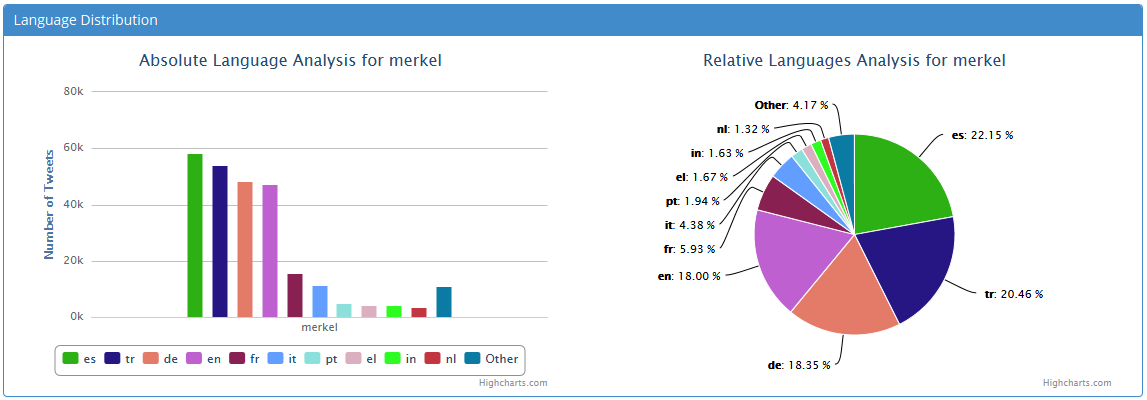
\includegraphics[width=\textwidth]{Bilder/Frontend/Screenshots/latestLanguageDistributionMerkel.png}
\caption{Sprachverteilung zu \glqq Merkel\grqq}
\label{fig:viewLanguageDistirbution}
\end{subfigure}
~
\begin{subfigure}[t]{0.45\textwidth}
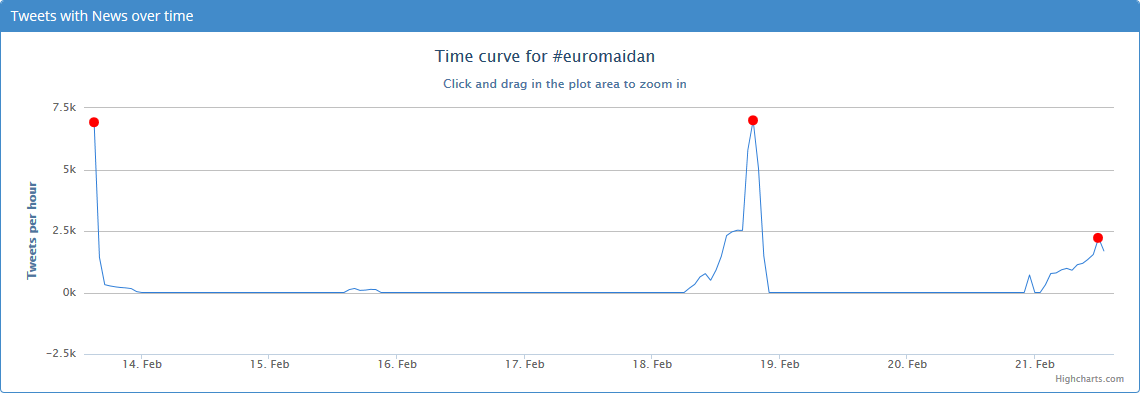
\includegraphics[width=\textwidth]{Bilder/Frontend/Screenshots/latestTweetsPerHourEuromaidan.png}
\caption{Anzahl Tweets im zeitlichen Verlauf zu \glqq \#euromaidan\grqq}
\label{fig:viewTweetsPerHour}
\end{subfigure}

\begin{subfigure}[t]{0.45\textwidth}
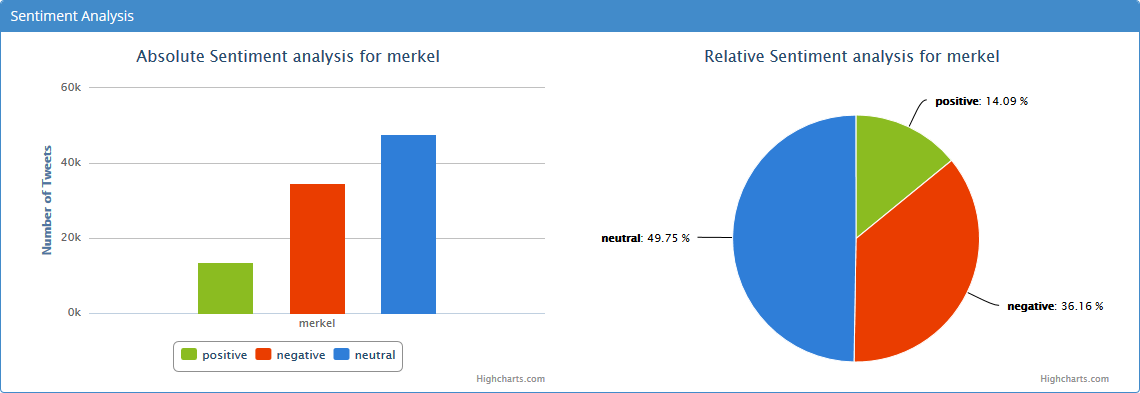
\includegraphics[width=\textwidth]{Bilder/Frontend/Screenshots/latestSentimentAnalysisMerkel.png}
\caption{Sentimentanalyse zu \glqq Merkel\grqq}
\label{fig:viewSentimentAnalysis}
\end{subfigure}
~
\begin{subfigure}[t]{0.45\textwidth}
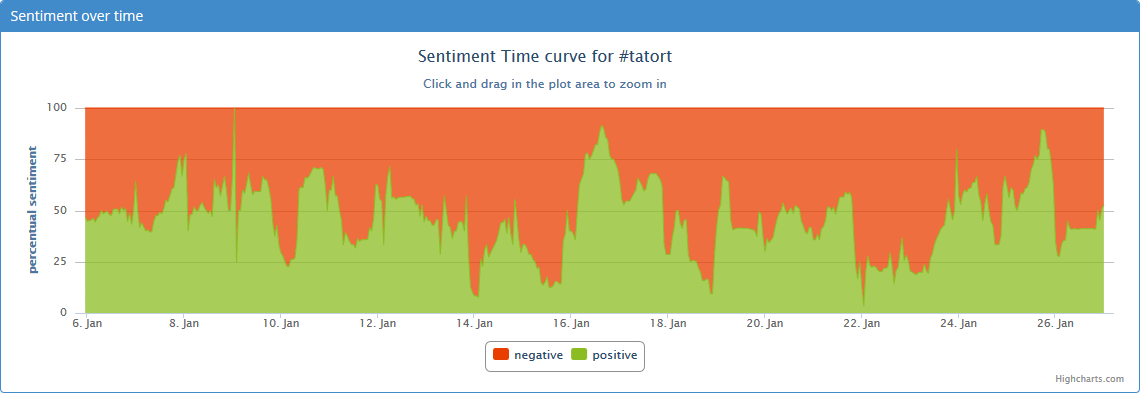
\includegraphics[width=\textwidth]{Bilder/Frontend/Screenshots/latestSentimentPerHourTatort.png}
\caption{Relatives Sentiment im zeitlichen Verlauf zu \glqq \#tatort\grqq}
\label{fig:viewSentimentPerHour}
\end{subfigure}

\begin{subfigure}[t]{0.45\textwidth}
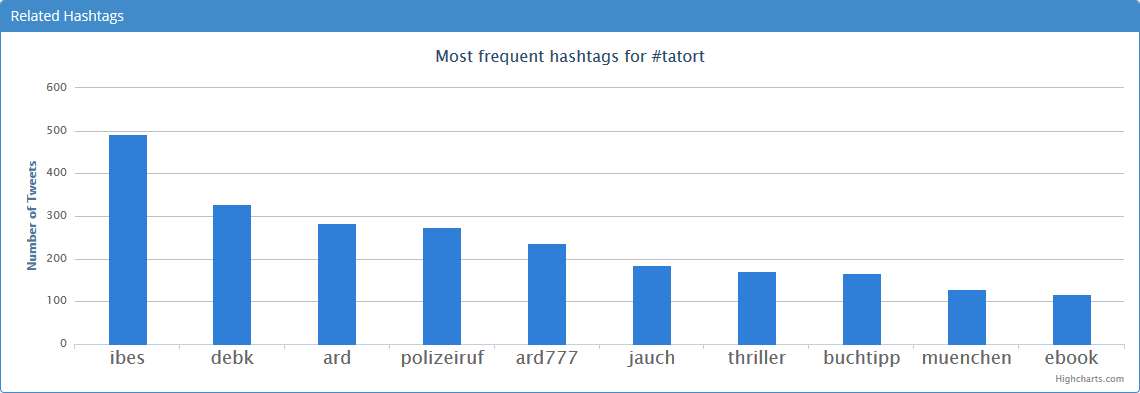
\includegraphics[width=\textwidth]{Bilder/Frontend/Screenshots/latestRelatedHashtagsTatort.png}
\caption{Verwandte Hashtags zu \glqq \#tatort\grqq}
\label{fig:viewRelatedHashtags}
\end{subfigure}
~
\begin{subfigure}[t]{0.45\textwidth}
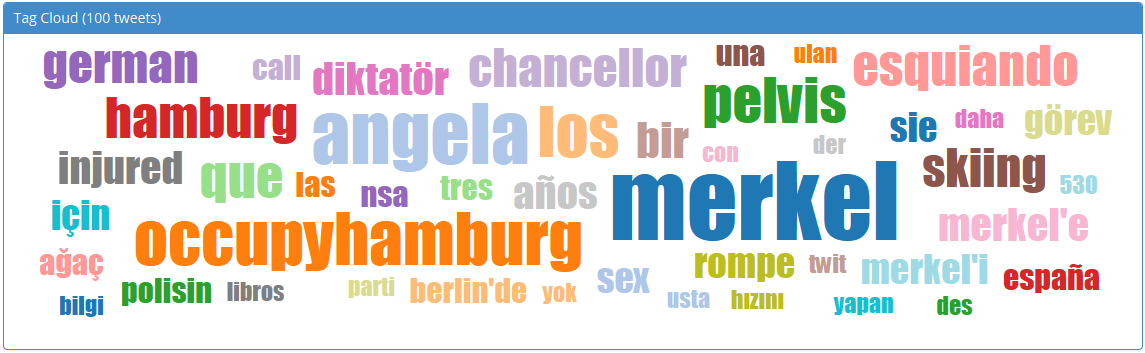
\includegraphics[width=\textwidth]{Bilder/Frontend/Screenshots/latestTagCloudMerkel.png}
\caption{Tag Cloud zu \glqq Merkel\grqq}
\label{fig:viewTagCloud}
\end{subfigure}

\begin{subfigure}[t]{0.45\textwidth}
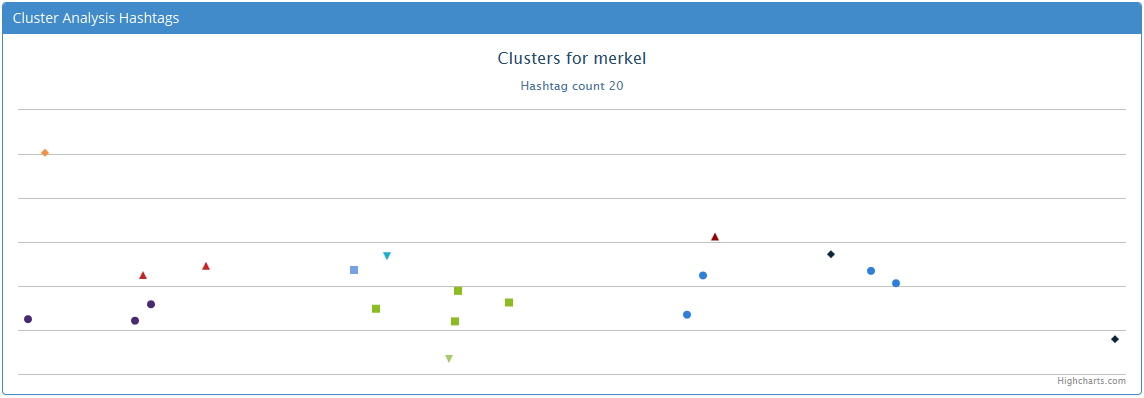
\includegraphics[width=\textwidth]{Bilder/Frontend/Screenshots/latestClusterHashtagMerkel.png}
\caption{Cluster-Analyse von Hashtags zu \glqq Merkel\grqq}
\label{fig:viewClusterHashtags}
\end{subfigure}
~
\begin{subfigure}[t]{0.45\textwidth}
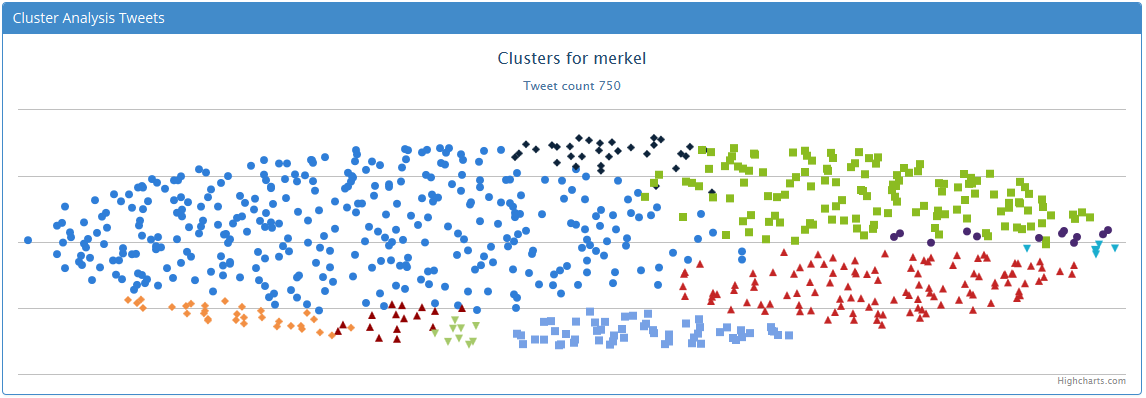
\includegraphics[width=\textwidth]{Bilder/Frontend/Screenshots/latestClusterTweetsMerkel.png}
\caption{Cluster-Analyse von Tweets zu \glqq Merkel\grqq}
\label{fig:viewClusterTweets}
\end{subfigure}
\caption{Alle acht Ansichten unseres Systems}
\label{fig:viewScreenshots}
\end{figure}

In der finalen Version unseres Systems sind acht verschiedene Ansichten enthalten, die in Abbildung \ref{fig:viewScreenshots} zu sehen sind. Fünf dieser Ansichten sind Umsetzungen der im vorigen Abschnitt beschriebenen, ursprünglichen Projektidee. Die drei weiteren Ansichten entstanden im Verlauf des Projektes auf Wunsch des Kunden, einen besseren Überblick über diesen Suchbegriff zu erhalten.
Das Stimmungsbild zu einem Thema wird in der \glqq Sentimentanalyse\grqq{} (\ref{fig:viewSentimentAnalysis}) betrachtet, bei der jedem Tweet eine positive, negative oder neutrale Stimmung (Sentiment) zugewiesen ist. Die zeitliche Ausbreitung ist in der Ansicht \glqq Tweets im zeitlichen Verlauf"' (\ref{fig:viewTweetsPerHour}) zu sehen, welche die Anzahl Tweets zum Suchbegriff pro Stunde auf einem Graphen aufträgt. Eine Kombination aus Stimmungsbild und zeitlicher Ausbreitung wird in der Ansicht \glqq Relatives Sentiment im zeitlichen Verlauf\grqq{} (\ref{fig:viewSentimentPerHour}) angeboten.
Das Clustering von Tweets gemäß ihrer Gemeinsamkeiten ist in der Ansicht \glqq Cluster-Analyse von Tweets\grqq{} (\ref{fig:viewClusterTweets}) umgesetzt worden. Eine Variation dieses Ansatzes findet sich in der \glqq Cluster-Analyse von Hashtags\grqq{} (\ref{fig:viewClusterHashtags}), bei der -- wie der Name schon vermuten lässt -- an Stelle von einzelnen Tweets Hashtags zu einem Suchbegriff zu Clustern zusammengefasst werden.
Die dort auftauchenden Hashtags sind allesamt Tweets zu diesem Suchbegriff entnommen. Eine Übersicht über die häufigsten dieser Hashtags bietet die Ansicht \glqq Verwandte Hashtags\grqq{} (\ref{fig:viewRelatedHashtags}), welche die zehn meistbenutzten Hashtags zum eingegeben Suchbegriff auflistet. Eine Verallgemeinerung dieser Ansicht ist die \glqq Tag Cloud\grqq{} (\ref{fig:viewTagCloud}), in der nicht nur Hashtags, sondern generell alle Worte (bis auf Worte ohne eigentlichen Informationsgehalt, sogenannte \textit{stop words}) ihrer Häufigkeit entsprechend angezeigt werden. Dabei wird die Häufigkeit eines Wortes durch die Größe der Darstellung repräsentiert: Je größer ein Wort dargestellt wird, desto häufiger ist es in Tweets zum analysierten Suchbegriff vorhanden. Außerdem existiert noch die \glqq Sprachverteilung\grqq{} (\ref{fig:viewLanguageDistirbution}), welche die absolute und relative Häufigkeit der Sprachen, in denen die Tweets eines Suchbegriffs verfasst sind, grafisch präsentiert.

Die Ergebnisse zu einem Suchbegriff werden in der Anzeige in einem Tab zusammengefasst, in dem die einzelnen Ansichten angezeigt werden. Bei der Suche nach weiteren Begriffen wird jeweils ein weiterer Tab hinzugefügt, der wiederum die einzelnen Ansichten enthält. Bei der Analyse von zwei oder mehr Suchbegriffen wird zudem ein weiterer Tab mit einer Vergleichsansicht aller eingegebenen Suchbegriffe präsentiert. Diese Vergleichsansicht enthält eine Ansicht zum Vergleich der Stimmungsbilder und eine Ansicht zum Vergleich der zeitlichen Verläufe der einzelnen Suchbegriffe, was in Abbildung \ref{fig:compare} zu sehen ist.

\begin{figure}[h!]
\centering
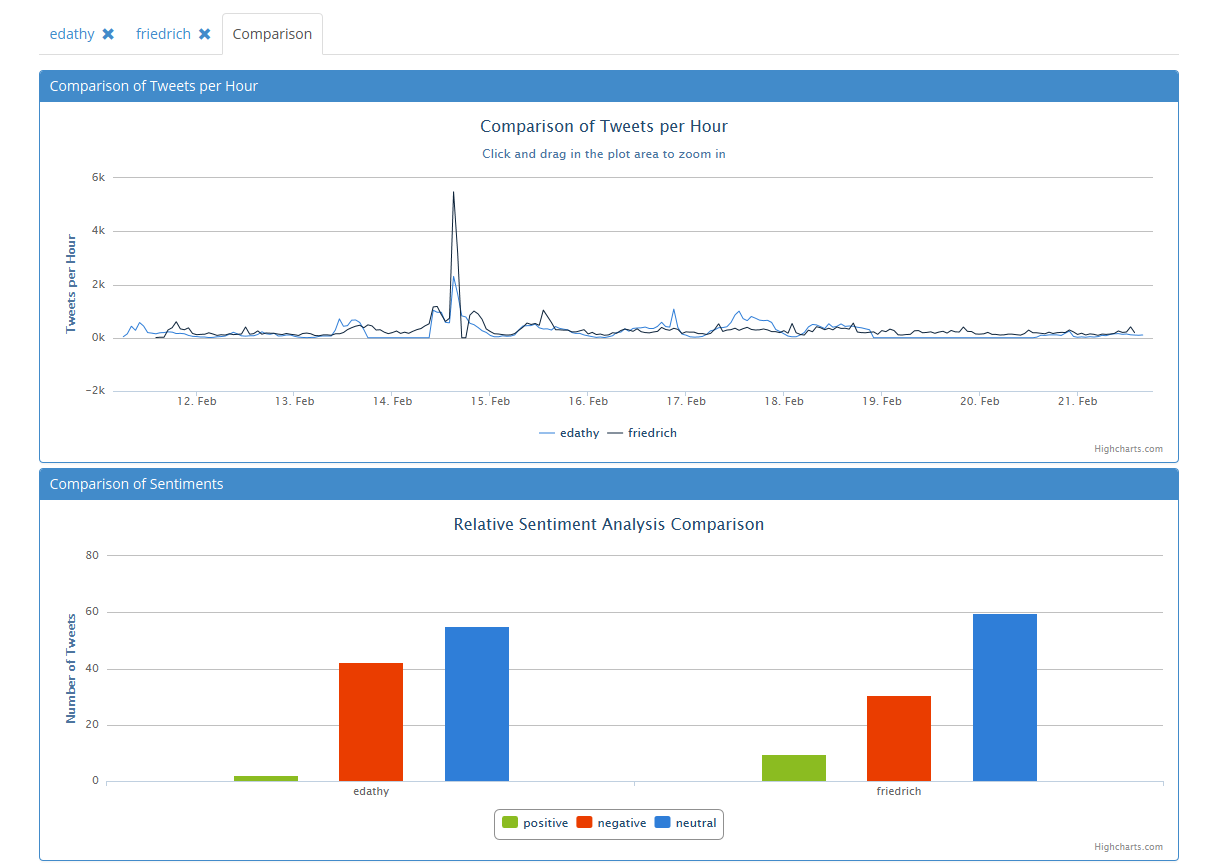
\includegraphics[width=0.8\textwidth]{Bilder/Frontend/Screenshots/comparison.png}
\caption{Vergleichsansicht zu den Suchbegriffen \glqq edathy\grqq{} und \glqq friedrich\grqq}
\label{fig:compare}
\end{figure}

Zusätzlich zur reinen Präsentation der analysierten Ergebnisse haben viele der soeben beschriebenen Ansichten auch Funktionalitäten, die exploratives Arbeiten mit dem System und den darin enthaltenen Daten ermöglicht. Beispielsweise ist es möglich, die zu analysierenden Daten zu einem Suchbegriff nach Sprachen zu filtern. Zusätzlich zum Sprachfilter in der Navigationsleiste ist diese Funktionalität auch aus der Ansicht \glqq Sprachverteilung\grqq\ verfügbar. Ebenso lässt sich die Suche nach einem weiteren Begriff nicht nur durch dessen Eingabe in die Suchleiste starten, sondern auch durch einen Klick auf den gewünschten Suchbegriff in der \glqq Tag Cloud\grqq\ oder bei \glqq verwandten Hashtags\grqq{}.
Eine Möglichkeit, detaillierte Informationen zu erhalten, bietet die Anzeige einzelner Tweets in unserem System. In der Ansicht zur \glqq Cluster-Analyse von Tweets\grqq\ ist dies durch einen Tooltip realisiert, in den Ansichten \glqq Sentimentanalyse\grqq\ und \glqq Tweets im zeitlichen Verlauf\grqq\ öffnet sich ein modaler Dialog mit einer detaillierten Anzeige von einzelnen Tweets.

Zusätzlich zur Anzeige einzelner Tweets bietet die Ansicht \glqq Tweets im zeitlichen Verlauf\grqq\ noch die Anzeige von News zu diesem Suchbegriff. Diese werden aus einer zusätzlichen Suche der drei externen Quellen \glqq Bing Web\grqq, \glqq Bing News\grqq\ und \glqq Google News\grqq\ akquiriert.
Dieses News-Modul wurde während des agilen Entwicklungsprozesses an Stelle des Kinomoduls umgesetzt, da eine Einbindung in das bis dahin bestehende System sowohl vom Product Owner, als auch von uns als sinnvoller erachtet wurde.
Eine weitere der ursprünglichen Projektideen, die aufgrund der Priorisierung durch den Product Owner herausfiel, ist die Anzeige der räumlichen Verbreitung von Tweets. Der Hauptgrund hierfür ist die relativ geringe Anzahl an Tweets, zu denen eine Position vorhanden ist.

In den folgenden Kapiteln wird das hier kurz beschriebene System und dessen Entstehungsprozess im Detail erläutert. Dazu wird in Kapitel \ref{cha:orga} zunächst beschrieben, wie wir das Projekt intern organisiert haben. Dies betrifft sowohl die Organisation des Systems als auch die von uns verwendete Vorgehensweise. Im darauf folgenden Kapitel \ref{cha:architektur} wird die Architektur unseres Systems beschrieben, welches in die drei grobe Bereiche Beschaffung, Analyse und Darstellung von Daten aufgegliedert ist. Die daraus entstandene Infrastruktur wird in Kapitel \ref{cha:infrastruktur} detailliert geschildert, woraufhin in Kapitel \ref{cha:komponenten} Details zu den einzelnen Komponenten und Ansichten gegeben werden. Das abschließende Kapitel \ref{cha:ausblick} fasst das zuvor Beschriebene kurz zusammen und bietet einen Ausblick auf mögliche weiterführende Ansätze, die auf dem von uns entwickelten System aufbauen.


\chapter{Projektorganisation}
\label{cha:orga}
\section{Ideenfindung}

Wie eingangs beschrieben stand zu Beginn des Projekts noch ein weites Feld an Themen und Anwendungen zur Verfügung. 
Um in diesem Feld ein konkretes Projektziel zu identifizieren, das innerhalb eines Projektseminars erreicht werden kann, teilte sich das Team in Absprache mit den Projektbetreuern in fünf Gruppen auf, die jeweils einen geeigneten Vorschlag für das Projekt erarbeiten sollten. 
Bei der Abstimmung über die Möglichkeiten kristallisierten sich dabei zwei Favoriten heraus. 
Anstatt uns vollständig für einen dieser Vorschläge zu entscheiden, kombinierten wir diese Alternativen. Damit sieht das Projekt in der finalen Fassung vor, das Meinungsbild auf Twitter zu einem bestimmten Thema aus einer Reihe von Gesichtspunkten darstellen zu können. 
Von der einen Projektidee stammen die Gesichtspunkte des zeitlichen Verlaufs, der räumlichen Verbreitung und der aktuellen Stimmungslage. Das Clustering von Tweets gemäß ihrer Gemeinsamkeiten bildete die zentrale Idee des anderen Vorschlages und wurde als weiter Gesichtspunkt aufgenommen.
Dies wurde um die Idee des ersten Vorschlags erweitert, Module anzubieten, welche die verfügbaren Daten in einem spezifischen Kontext interpretieren und dabei auch weitere externe Daten heranziehen. Als konkretes Modul sollte dabei ein sogenanntes "`Kinomodul"' implementiert werden, welches Informationen aus externen Filmdatenbanken mit den Ergebnissen aus Twitter kombiniert, um Filme vergleichen zu können und Empfehlungen möglich zu machen.
\section{Scrum}
Wie bereits erwähnt, wurde für die Organisation des Projektes auf Hilfsmittel aus der agilen Softwareentwicklung zurückgegriffen. Im Gegensatz zur klassischen Softwareentwicklung z.\,B. nach dem Wasserfallmodell mit teils langen Phasen, sind die Hauptmerkmale der agilen Softwareentwicklung vor allem flexiblere und oftmals vor allem zeitlich weniger aufwändige Methoden. Im Vordergrund stehen neben weiteren Merkmalen Schlagwörter, wie z.\,B. kurze Iterationen, testgetriebene Entwicklung oder häufige Refaktorierungen. %TODO: evtl umformulieren... -> würde das nicht explizit Schlagwörter nennen und vielleicht auch das "weitere Merkmale" weglassen
Die Anzahl der Methoden, die sich unter dem Stichwort agile Softwareentwicklung zusammenfassen lassen, ist relativ groß, sodass sich kaum sämtliche Methoden konsequent innerhalb eines Projektes umsetzen lassen. Es haben sich daher verschiedene Vorgehensmodelle, wie z.\,B. Extreme Programming, Kanban oder Scrum entwickelt. Da wir für die Projektorganisation die Methoden aus Scrum verwendet haben, möchten wir im Folgenden einen Überblick darüber geben, welche Methoden von uns angewandt wurden und auf welche wir aus welchen Gründen verzichten mussten.

\subsection{Grundmerkmale}
Ohne Scrum an dieser Stelle im Detail erklären zu wollen, seien einige wichtige Grundmerkmale genannt, welche sich auch in unserem Projektseminar wiedergefunden haben.

Im Rahmen von Scrum werden die Anforderungen zunächst grob als sogenannte User Stories formuliert und anschließend in möglichst spezifische einzelne Teilaspekte (sogenannte Arbeitspakete) unterteilt. Nachdem die Projektidee ausgereift ist, wird dies innerhalb des Teams im Sinne von Scrum umgesetzt. Anschließend werden die Aufwände der Arbeitspakete innerhalb des Teams geschätzt. Details hierzu folgen in einem der nächsten Abschnitte.

Da das Vorgehen über die komplette Entwicklungszeit nicht aus einzelnen langen und aufeinander folgenden Phasen (wie z.\,B. im Wasserfallmodell) besteht, sondern bei Scrum auf kurze ca. 2-3 Wochen dauernde und wiederholende Iterationen gesetzt wird, folgt nach der Aufwandschätzung das Aufteilen der vorhandenen User Stories auf die jeweils kommende Iteration.
Das von Scrum erklärte und von uns in der Regel erreichte Ziel ist hierbei, am Ende einer jeden Iteration ein funktionsfähiges Stück Software in der Hand zu halten.

Ein weiteres erklärtes Grundprinzip von Scrum ist eine rege Kommunikation, gestützt durch häufige und verschiedene Arten von Meetings. Auch wir konnten im Rahmen des Projektseminars mit den verschiedenen Arten von Meetings unsere Erfahrungen sammeln.

In Kombination mit den kurzen Iterationen und dem Endziel einer jeden Iteration führt dies dazu, dass das Entwicklungsteam schnell auf (sich ggf. ändernde) Kundenwünsche reagieren kann und so mögliche und vor allem langfristig folgenreiche Missverständnisse in großen Teilen verhindert werden können. Auch auf unser Projektteam kamen im Rahmen der Entwicklung einige neue Kundenwünsche zu, welche zumeist erfolgreich und zeitnah umgesetzt werden konnten.

Um den Erfolg von Scrum sicherzustellen, ist auf die Einhaltung dieser Grundprinzipien zu achten. Soweit dies im Rahmen einer Lehrveranstaltung möglich ist, wurde dies vom Projektteam auch gemacht, sodass man festhalten kann, dass Scrum für unser Projekt definitiv ein Erfolg war.

Um die Grundprinzipien und die Umsetzung innerhalb unseres Projektes ein wenig weiter zu beleuchten, werden wir im Folgenden auf einige Rollen und Methoden im Detail eingehen.


\subsection{Rollen}
\subsubsection{Scrum-Team}
Innerhalb des Scrum-Modells gibt es verschiedene Rollen. Die Projektteammitglieder nahmen hierbei natürlich in erster Linie die Rolle der Entwickler ein. Das Entwicklerteam wird bei Scrum auch als Scrum-Team bezeichnet. Ein wichtiges Merkmal ist, dass dieses Team in großen Teilen selbstverwaltet arbeitet und eventuell auftretende Probleme intern zu lösen versucht. Dies hat bei uns sehr gut funktioniert. So wurden die verfügbaren Aufgaben ohne Komplikationen innerhalb des Teams verteilt und auch ein auftretendes Kommunikationsproblem konnte autark innerhalb des Teams gelöst werden.

\subsubsection{Product Owner}
Die Rolle des Product Owners ist am ehesten mit der eines Projektleiters oder Firmeninhabers in einem klassischen Szenario zu vergleichen. Der Product Owner ist derjenige, der das fertige Produkt nach außen verkauft und mit dem Kunden in engem Kontakt steht. Letztendlich nimmt er daher immer auch die Rolle eines Vermittlers zwischen Kunden und Entwicklern ein, die ansonsten nicht unbedingt in direktem Kontakt miteinander stehen müssen.

In unserem Szenario wurde diese Rolle durch einen unserer Projektbetreuer besetzt. Er wohnte in dieser Rolle z.\,B. den sogenannten Sprint-Planning-Meetings bei und sortierte in diesen Meetings die gefundenen User Stories nach einer Priorität im Sinne des Kunden. Generell fanden im Rahmen des Projektseminars regelmäßige Meetings mit dem Product Owner statt, welche je nach aktueller Situation innerhalb der Iteration verschiedene Ausprägungen erhielten und somit nicht nur zum Sprint Planning wurden, sondern z.\,B. auch zum Sprint Review wurden.

\subsubsection{Scrum Master}
Der Scrum Master ist mit dem Entwicklerteam eng verbunden, aber stellt eigentlich kein Mitglied des Entwicklerteams, sondern eine Art Bindeglied zum Product Owner dar. Der Scrum Master hält dem Entwicklerteam den Rücken frei und sorgt z.\,B. dafür, dass die benötigten externen Anforderungen erfüllt sind. Damit hat er vor allem zu Beginn eines Projektes einen etwas erhöhten organisatorischen Aufwand zu bewältigen und nimmt in der restlichen Zeit eine eher moderierende Rolle in den verschiedenen Meetings ein. Normalerweise wechselt im Verlaufe eines Projektes der Scrum Master nicht, sondern wird durchgehend durch die selbe Person repräsentiert. Damit alle Projektmitglieder aber einmal in die Position des Scrum Masters kommen konnten, mussten wir mit diesen Prinzipien leider brechen. Der Scrum Master war also bei uns abweichend von Scrum sowohl durch wechselnde Personen repräsentiert als auch stets ein Mitglied des Entwicklerteams. Das tat dem Moderieren der verschiedenen Meetings aber keinen großen Abbruch, sodass letztendlich alle Projektteammitglieder von den Einblicken in diese Rolle profitiert haben.

\subsubsection{Kunde}
Als weitere Rolle gibt es natürlich den Kunden, welcher in unserem Szenario durch den anderen Projektbetreuer verkörpert wurde. Der Kunde stellt natürlich die anfänglichen grundsätzlichen Anforderungen an das Projekt und beauftragt das gesamte Team mit der Entwicklung. Obwohl die Projektidee in diesem Fall durch das Projektteam selbst entwickelt wurde, hat der Kunde es sicht nicht nehmen lassen im Verlauf des Projektes ändernde Anforderungen einzubringen, wie z.\,B. dem Wunsch nach einem "'Kachelinterface"'. Im eigentlich Scrum-Sinne interagiert der Kunde nur bedingt mit dem gesamtem Entwicklerteam, hiervon wurde im Rahmen des Projektseminars ebenfalls ein wenig abgewichen. Dies hat aber insgesamt zu keiner negativen Beeinflussung im Sinne von Scrum geführt und sich teilweise durch kurze Kommunikationswege eher als Vorteil herausgestellt.


\subsection{Verwendete Methoden}
\subsubsection{User Story}
Die einzelnen Aufgabenkomplexe werden als User Stories bezeichnet, entsprechen also einer eher umgangsprachlichen Formulierung aus der Sicht des Benutzers, was in der Anwendung konkret passieren soll.
Konkretisiert werden diese User Stories durch die Entwickler in dem sie auf kleinere konkrete Aufgaben, sogenannte Tasks unterteilt werden.
User Stories als auch Tasks wurden von uns auf (unterschiedlich großen) Karteikarten festgehalten, um diese später flexibel dem Scrum-Board hinzufügen zu können. Details zum Scrum-Board folgen in einem späteren Abschnitt.

Folgende beispielhafte User Story wurde verfasst, um die Tag-Cloud-Anzeige zu implementierten:
\begin{center}
\begin{tabular}{|lll|} \hline
2.4 & \multicolumn{2}{c|}{Als Benutzer möchte ich Tag-Clouds haben} \\
    &                     &           \\
    & \small{Geschätzter Aufwand} & \small{5 Punkte}  \\
    & \small{Benötigte Stunden} & \small{29}     \\ \hline
\end{tabular}
\end{center}
In der Abbildung \ref{fig:viewTagCloud} ist die Implementierung im Frontend abgebildet.
Für die Implementierung der Tag Cloud wird eine REST-Anfrage benötigt, die die benötigten
Datenbank\-anfragen macht, sowie die 
Visualisierung im Frontend.
Deswegen wurde die User Story in folgende Tasks aufgebrochen:
\begin{center}
\begin{tabular}{|lll|} \hline
2.4.1 & \multicolumn{2}{c|}{REST-Anfrage implementieren} \\
    &                     &           \\
    & \small{Aufwand} & \small{2 Punkte}  \\ \cline{2-3}
    & \multicolumn{1}{|l}{\small{Beteiligte Personen}} & \small{Benötigte Stunden} \\ 
    & \multicolumn{1}{|l}{\small{Person1}}             & \small{2}                    \\
    & \multicolumn{1}{|l}{\small{Person2}}             & \small{4}                    \\
\hline
\end{tabular}
\end{center}
\begin{center}
\begin{tabular}{|lll|} \hline
2.4.2 & \multicolumn{2}{c|}{Visualisierung im Frontend implementieren} \\
    &                     &           \\
    & \small{Aufwand} & \small{3 Punkte}  \\ \cline{2-3}
    & \multicolumn{1}{|l}{\small{Beteiligte Personen}} & \small{Benötigte Stunden} \\ 
    & \multicolumn{1}{|l}{\small{Person2}}             & \small{12}                    \\
    & \multicolumn{1}{|l}{\small{Person3}}             & \small{11}                    \\
\hline
\end{tabular}
\end{center}

\noindent
An der Nummerierung oben links erkennt man, dass die User Story und die Tasks zu der zweiten Iteration gehören, die User Story
hat die Nummer vier, wobei die Nummerierung keine besondere Rolle spielt und lediglich der eindeutigen Identifizierung dient.  Die Tasks haben entsprechend die Nummern eins und zwei. 

Auf den User-Story-Karten wurde protokolliert, wie hoch der Aufwand in Punkten (hier 5) dieser Story ist, welcher sich durch die Summe des Aufwandes der einzelnen Tasks ergibt. In diesem Fall 2 Punkte für den Task 2.4.1 und 3 Punkte für den Task 2.4.2. 
Ebenfalls wurde an den User Stories notiert, wie hoch der benötigte Aufwand in Stunden tatsächlich ist. Dieser setzt sich wie die Punkte aus der Summe der benötigten Stunden für die einzelnen Tasks zusammen, welche von dem jeweiligen Entwickler nach Fertigstellung eines Tasks auf der Task-Karteikarte festgehalten wurde.

Durch diese Art der Buchführung über verbrauchte Punkte und Stunden, ist es relativ einfach möglich, den jeweils aktuellen Fortschritt innerhalb der Iteration zu kontrollieren und sich einen Überblick darüber zu verschaffen, ob am Ende der Iteration alle Tasks und Stories fertig sind oder ob noch etwas offen bleiben wird. Mehr dazu später im Abschnitt über den Burndownchart.

\subsubsection{Planning Poker}
Im Gegensatz beispielsweise zum Wasserfallmodell wird bei Scrum der Aufwand nicht vom Projektleiter oder Geschäftsführer bestimmt und quasi "`von oben"' diktiert, sondern der Aufwand für die Implementierung verschiedener Anforderungen wird aus dem Team heraus bewertet und geschätzt. Hierzu bedienen sich die beteiligten Entwickler einem Schätzverfahren, das unter dem Namen Planning Poker bekannt ist. Als Referenz-Aufwand wird eine im Team bekannte Aufgabe heran gezogen, anhand derer der Aufwand einer neuen Anforderung geschätzt werden soll. Der Hauptvorteil des Planning Pokers liegt darin, dass die beteiligten Personen sich zunächst nicht gegenseitig beeinflussen und daher trotz der allgemein bekannten Referenz-Aufgabe sehr abweichende Schätzungen entstehen können. 
Diese abweichenden Schätzungen eröffnen dann Diskussionen über den tatsächlichen Umfang und Aufwand der Aufgaben. Dies hatte auch bei uns im Projektteam die Folge, dass bei nicht-trivialen Aufgaben der Sachverstand aller Mitglieder einging und damit für jeden eine genauere Kenntnis der Anforderungen erreicht wurde.

Wie wir anhand der User Stories und einzelnen Tasks bereits gesehen haben, wird dieser Aufwand in Punkten geschätzt, wobei Punkte bei Scrum ausdrücklich nicht den Arbeitsstunden entsprechen, sondern als eine Art Einschätzung der Komplexität der Aufgabe zu verstehen sind. Dies ist von Vorteil, wenn sich Entwickler mit unterschiedlichen Erfahrungswerten an die selbe Aufgabe machen und sicherlich unterschiedliche Zeit benötigen würden. Da der Punktestand gemessen werden kann, bietet dies einen besseren Überblick über den Fortschritt der Iteration.

Die Summe der geschätzten Teilaufgaben und User Stories landen gesammelt in dem Product Backlog, welches somit das Pendant zu dem sonst bekannten Pflichten- oder Lastenheft darstellt. Das Pendant zu dem Product Backlog war in unserem Fall die Sammlung der noch nicht geplanten User Stories, welche auf Karteikarten notiert wurden, um diese inklusive der zugehörigen Tasks, an unserem Scrum-Board anbringen zu können.


\subsubsection{Scrum-Board}
Das Scrum-Board ist eine Art Tafel oder White-Board, welches an einer für alle Beteiligten gut sichtbaren Stelle aufgehängt wird. Es ist ein sehr essenzieller Bestandteil von Scrum und dient dazu, einen Überblick über den Fortschritt der einzelnen Aufgaben zu geben, sowie den Entwicklern die Möglichkeit zu geben sich flexibel noch nicht bearbeitete Aufgaben heraus zu nehmen.
Aus der durch den Product Owner priorisierten Liste von User Stories aus dem Sprint Backlog, kann nun eine Story heraus gegriffen und an dem Scrum-Board angebracht werden. Dies signalisiert jedem, dass aktuell daran gearbeitet wird. Die einzelnen Arbeitspakete können aber dennoch von unterschiedlichen Entwicklern bearbeitet werden. Eine Idee von Scrum ist, dass sich ein Entwickler hier durchaus auch mal eine Aufgabe aus einem Gebiet nehmen kann, in dem er nicht unbedingt vollständig eingearbeitet ist, um so seinen eigenen Horizont zu erweitern und auch durch einen anderen Blickwinkel der Entwicklung dieser User Story evtl neue Impulse hinzuzufügen.
Aufgrund steigender Komplexität der einzelnen Komponenten hat dieser Fachgebiets-Wechsel-Effekt im Laufe des Projektes nach und nach abgenommen, was jedoch durchaus zu erwarten war.
Generell war der Überblick der offenen, geschlossenen und in Bearbeitung befindlichen Stories und Tasks jedoch sehr hilfreich.

\subsubsection{Burndownchart}
Neben dem Scrum-Board ist das Burndownchart ein eben so wichtiger Bestandteil von Scrum. Immer wenn am Scrum-Board eine Aufgabe aus dem Bereich der die in Bearbeitung befindlichen Stories und Tasks kennzeichnet, heraus genommen wird, wird der in Punkten auf der Story notierte Aufwand von der Summe der Aufwände der Iteration abgezogen und ein Restwert des Aufwandes wird ermittelt. Dieser Ist-Wert des Rest-Aufwands wird anschaulich an einer Kurve dargestellt, welche als Burndownchart bezeichnet wird.
Idealer Weise verläuft diese Kurve möglichst nah an einer gedachten (und je nach Ausprägung auch eingezeichneten) Ideallinie, welche diagonal von 100\% des Aufwandes bis zu 0\% über den zeitlichen Verlauf der Iteration verläuft. In der Praxis liegt diese Linie doch oftmals oberhalb dieser Ideallinie, da Stories erst nach Beendigung vollständig von dem Rest-Wert abgezogen werden und da durch Probleme die im Verlauf der Iteration auftreten, die Summe des Gesamtaufwandes oft noch ansteigen kann. Um dies besser zu visualisieren haben wir eine weitere Linie in unserem Burndownchart eingeführt, welche den 100\% Wert des Aufwandes darstellt und an entsprechenden Stellen dann einen Knick nach oben bekommt.
Somit konnte man sich dennoch einen guten Überblick darüber verschaffen, wie gut man mit den geplanten Aufgaben dieser Iteration im Zeitplan ist.


\subsubsection{Definition of Done und Testgetriebene Entwicklung}
Wie im vorherigen Abschnitt beschrieben, konnte man unserem Scrum-Board stets entnehmen, welche Aufgaben bereits abgeschlossen sind. Damit sich zwischen den Mitgliedern keine unterschiedlichen Auffassungen etablieren, wann eine Aufgabe als abgeschlossen bezeichnet werden kann, sieht Scrum eine sogenannte \textit{definition of done} (DoD) vor. Eine solche DoD wurde vom Team innerhalb der ersten Wochen erarbeitet und stellte seitdem ein verbindliches Regelwerk dar. Vor allem war ein fester Bestandteil der DoD, dass die jeweilige Komponente getestet worden sein soll, bevor die Aufgabe als abgeschlossen bezeichnet werden kann. Dies wurde durch automatisierte Tests erreicht, worüber in einem kommenden Abschnitt noch mehr zu erfahren sein wird.

\subsection{Scrum, But}
Da bislang die Scrum-Methoden betrachtet wurden, welche vollständig oder zumindest in großen Teilen nach Scrum-Vorgabe durch uns genutzt und umgesetzt wurden, möchten wir noch auf einige Aspekte eingehen, welche in unseren Augen nur teilweise bzw. mit einigen Abweichungen von uns genutzt wurden.
\subsubsection{Daily Scrums}
Diese Form von Meeting sollte wie der Name schon andeutet täglich stattfinden. Da sich aber kaum ein täglicher fixer Termin finden ließ, an dem stets alle oder zumindest die meisten Teammitglieder hätten anwesend sein können, wurde innerhalb unseres Team hieraus ein D-Daily-Scrum gemacht, % d-daily? - A: sic! :P aber von mir aus, schmeisst es raus oder formuliert es um. Mir gefällts so!
 sodass wir uns lediglich Dienstags und Donnerstag zu dieser Art von Meeting zusammen gefunden haben.
Inhaltlich geht es beim Daily Scrum eigentlich darum, dass jedes Mitglied kurz darlegt, was seit dem letzten Daily-Scrum geschehen ist, also letztendlich was entwickelt wurde und was bis zum nächsten Daily Scrum geschehen soll. Ebenfalls sollte kurz erwähnt werden, ob mögliche Komplikationen zu erkennen sind, welche das Ziel bis zum nächsten Daily Scrum gefährden könnten. Dies würde der Scrum Master dann zum Anlass nehmen, aktiv zu werden um die möglichen Hindernisse aus dem Weg zu räumen.

Um den Charakter eines Kurz-Meetings zu stärken und nicht in langwierige Diskussionen abzudriften, wird empfohlen, diese Art von Meetings im Stehen abzuhalten, möglichst auch außerhalb des regulären Arbeitsbereiches. Dies wurde vom Team auch umgesetzt, indem man sich im Erdgeschoss des Institutes traf und besagte Punkte ansprach. Vermutlich aufgrund der nicht täglich stattfindenden Daily-Scrum-Meetings neigten die Meetings teilweise zu längeren Diskussionen und übertrafen dann definitiv die reine Bestandsaufnahme.

\subsubsection{Retrospektive und Sprint Review}
Aufgrund der eingeschränkten Anzahl an gemeinsamen Terminen pro Woche ließen sich die Retrospektiven und Sprint Reviews leider nicht immer vollständig so umsetzen, wie es in Scrum eigentlich vorgesehen ist. Es fanden zwar vergleichbare Termine statt, aber es war selten der Fall, dass eine Retrospektive im Scrum-Sinne zur Selbstreflektion des Entwicklerteams genutzt wurde und einen eigenständigen Termin zu dem Sprint Review darstellte. Meist war das Meeting zum Ende eines Sprints eine Mischform dieser beiden Scrum-Bestandteile.
Dem grundsätzlichen Scrum-Ablauf hat dies in unserem Szenario jedoch keinen Abbruch getan, sodass Scrum für uns dennoch sehr gut funktioniert hat.

\subsubsection{User-Story}
Die Aufgaben wurden als User Stories verfasst (aus Sicht des Benutzers) und 
anschließend in Tasks (kleinere Aufgaben) aufgebrochen. 
Diese wurden auf Karteikarten geschrieben und dem Scrum-Board hinzugefügt. 

\section{Technologien}
\label{sec:Tech}
Die bei unserem Projektseminar eingesetzten Technologien wurden zum größten Teil auf Grund von persönlicher Erfahrungen eines oder mehrerer Teammitglieder ausgewählt. Die Entscheidung, unser Programm hauptsächlich mit Java zu schreiben, beruht allein auf der Tatsache, dass alle Teammitglieder ausreichend viel Erfahrung mit dieser Programmiersprache hatten. Die Entscheidung für Java als Programmiersprache führte bei den Recherchen bezüglich der Kommunikation mit der Twitter-API zu der Java-Bibliothek Twitter4J \cite{Twitter4J}. Diese kapselt die Kommunikation mit Twitter komplett und liefert die Ergebnisse einer Anfrage an Twitter als einfaches Java-Objekt.

Die Entscheidung für eine bestimmte Datenbank war ebenfalls von Vorwissen im Team geprägt. MySQL ist die Datenbank, mit der alle Mitglieder bereits erste Erfahrungen gemacht hatten. Eine tatsächliche Evaluierung der zur Verfügung stehenden Datenbanken wurde nicht durchgeführt. Eine Auswahl einer Datenbank, die auf unsere Anforderungen besser spezialisiert ist, hätte allerdings unter Umständen aufgetretene Performanceprobleme besser lösbar gemacht.

Die Entscheidung, die Ausgabe unserer Analysen in einer Webseite darzustellen, begründet sich zum einen auf dem expliziten Wunsch des Teams, dies in unser Projekt mit aufzunehmen. Zum anderen erschien dem Team eine Benutzeroberfläche für eine Java-Applikation nicht zeitgemäß. Daher wurde entschieden, für das Frontend JavaScript in Verbindung mit jQuery \cite{jQuery} zu verwenden. Die Graphen in unserer Anzeige wurden mit dem Framework Highcharts erstellt \cite{Highcharts}. Die Entscheidung für Highcharts beruhte in erster Linie wieder auf vorher vorhandene Erfahrungen einiger Teammitglieder. Dieses Framework ermöglicht, es einfache Graphen schnell und unkompliziert zu erstellen. Für die komplexeren Anzeigen, wie zum Beispiel die Tag-Cloud, wurde nach einer Recherche das Framework Data-Driven Documents (D3) verwendet \cite{d3}. Diese umfangreiche Visualisierungsbibliothek löst das Problem einer Visualisierung von Daten allerdings mit einer anderen Herangehensweise als Highcharts. Hierbei werden dem Entwickler alle Werkzeuge an die Hand gegeben, die benötigt werden, um eine beliebige Vektorgrafik zu erstellen und zu animieren.

\section{Code-Organisation}
Wie im vorherigen Kapitel beschrieben verlässt sich unser Projekt an vielen Stellen %TODO: echt? Wo wurde das denn vorher beschrieben?
auf externe Bibliotheken. Um einen reibungslosen Entwicklungsablauf innerhalb des Teams 
zu erreichen, muss eine Methode bereitgestellt werden, welche die Verwaltung dieser 
externen Bibliotheken übernimmt. Diese Aufgabe wird für Java-Projekte von dem 
Programm Maven der Apache Foundation übernommen. 
%TODO Quelle

Bei diesem Programm handelt es sich um ein plattformunabhängiges Build-Management-Tool 
für Java-Projekte, das die Entwickler beim Anlegen, Kompilieren, Testen und 
Verteilen des Projekts unterstützt. Ein Großteil dieser Schritte soll automatisiert 
erledigt werden. Die Konfiguration all dieser Funktionen wird in einer XML Datei 
(\texttt{pom.xml}) festgehalten. An dieser Stelle lassen sich auch alle Abhängigkeiten zu 
externen Bibliotheken eintragen. Diese werden bei dem Kompilier-Befehl aus einem 
zentralen Repository in die Entwicklungsumgebung geladen, sowie alle Build-Path-Parameter entsprechend für das Projekt gesetzt. Dies erlaubt es, externe Bibliotheken 
in sehr einfacher Art und Weise in ein Projekt einzubinden, ohne einen komplizierten 
Importierungsprozess für den einzelnen Entwickler zu erfordern.

In dieser XML-Datei können ebenfalls die Optionen für die Tests des Projekts gesetzt 
werden. Über ein Plugin für verschiedene Entwicklungsumgebungen (Eclipse, IntelliJ) 
können die Konfigurationsdateien für diese Programme sehr einfach erstellt werden. 
Über Plugins der Entwicklungsumgebungen ist es allerdings auch möglich, Maven-Projekte 
in die Programme zu importieren. 

In den ersten Wochen unseres Projektseminars wurden die beiden Komponenten Daemon und 
REST-Service als zwei separate Maven-Projekte angesehen. Erst als die 
Regressionsmodelle eine Verbindung zwischen den beiden notwendig gemacht haben, musste 
die Konfiguration umgestellt werden. Ein erster Versuch sah vor, das Daemon-Projekt lokal in das Maven-Repository zu installieren und es dann als direkte Abhängigkeit in das REST-Service-Projekt mit aufzunehmen. Diese Herangehensweise erwies sich aber als nicht praktikabel, da beim Kompilieren des REST-Service-Projekts der Code für die Daemon-Klassen nur dann neu aus dem Repository geladen wurde, wenn es sich um eine neue Version des Projekts handelte. Eine neue Versionsnummer für das Projekt musste allerdings vor jedem Kompilieren per Hand gesetzt werden. Aus diesem Grund wurde dieser Ansatz verworfen. Eine Lösung für dieses Problem konnte mit dem Modul-Plugin für Maven erreicht werden. Hierbei werden mehrere Maven-Projekte als einzelne Module unter einem übergeordneten Projekt zusammengefasst. Der essentielle Punkt ist hierbei, dass ein Unterprojekt von einem anderen abhängig sein darf. Diese Konfiguration erlaubte es, die beiden Projekte nacheinander zu kompilieren und den REST-Service abhängig vom Daemon zu machen. Somit sind die Klassen des Daemon-Projekts auch im REST-Service nutzbar. Dies bedeutet ebenfalls, dass für einen 
Kompilierungsvorgang des gesamten Projekts sowohl die Tests im Daemon- als auch im 
REST-Service-Modul durchlaufen werden müssen. Um diese Tests unabhängig vom 
Entwicklungssystem bzw. unabhängig von dem gerade verwendeten Computer durchführen zu 
können, mussten einige Vorkehrungen getroffen werden.

\section{Tests}
Wie vorher erwähnt, ist eine Komponente der Softwareentwicklung, die über Maven 
automatisiert abläuft, das Testen. Bei dem Kompilierungsvorgang führt Maven ebenfalls 
alle Tests aus, die sich in einem vorher definierten Unterordner des Projekts 
befinden. Maven arbeitet hier nahtlos mit JUnit zusammen, um alle Tests in der 
entsprechenden Konfiguration durchzuführen.

Für den REST-Service waren vor allem die Integrationstests von essentieller 
Wichtigkeit. Hier wurden die verschiedenen Anfragen getestet, welche die Ergebnisse and 
das Frontend weiterreichen sollten. Um eine unabhängige Testumgebung zu erreichen, 
wurde hier eine explizite Testdatenbank eingerichtet, die vor allen Tests einmal 
aufgebaut wird. Hierzu wurde eine Datenbank per Hand bearbeitet und in eine Datei 
exportiert, die alle SQL-Anweisungen beinhaltet, um die Datenbank neu zu erstellen. 
Diese Datei konnte als Ressource in das Projekt eingebunden werden und ebenfalls zur 
Versionskontrolle hinzugefügt werden. Diese Dump-Datei musste noch für die lokale 
Datenbank angepasst werden. Der Name der Datenbank, der sich in der Dump-Datei 
befindet musste durch den in der \texttt{database.properties}-Datei ersetzt werden. Diese 
Vorkehrungen ermöglichten es, in den darauffolgenden Tests von einer sehr spezifischen 
Datenbank ausgehen zu können und somit komfortabel Tests zu erwarteten und 
unerwarteten Eingaben durchzuführen. Neben den Integrationstests wurden auch viele 
Methoden, die Datenbankabfragen weiterverarbeiten, mit Unit-Tests getestet. Auch hier 
wurden Randbedingungen, wie zum Beispiel leere Arrays, mit überprüft. Weitere Informationen zu den Besonderheiten des REST-Service sind im Infrastruktur-Kapitel bzw. in den Kapiteln der einzelnen Module zu finden.

Die Tests im Daemon, die eine externe Datenbank voraussetzen, wurden ebenfalls mit einer extra Datenbank realisiert. Es wurde erneut eine Datenbank per Hand erstellt und ein Dump erzeugt, der in die Versionierung mit aufgenommen wurde. Bei den Integrationstests wurde hauptsächlich getestet, ob von Twitter abgefragte Informationen korrekt in die Datenbank übertragen wurden. Da ein Teil der Sentimentanalyse auch im Daemon stattfindet, müssen die Unit-Tests für diese ebenfalls im Daemon Projekt abgehandelt werden. Eine weitere Komponente des Daemons, die ausgiebig getestet wurde, ist das Multithreading. Mehr Details zu der Funktionsweise des Multithreading und den Testfällen sind im Hauptkapitel des Daemons zu finden.


\chapter{Architektur}
\label{cha:architektur}
Aus der zuvor beschriebenen Projektidee ergeben sich drei Aufgabenbereiche von TMetrics: die Beschaffung und Filterung der Daten von Twitter, ihre Analyse durch Verfahren innerhalb von TMetrics (beispielsweise das Clustering oder die Analyse des Meinungsbildes) und die abschließende Darstellung der Resultate für den Benutzer in einer Browser-Anwendung (im Folgenden auch als Frontend bezeichnet). Die daraus resultierende Grundstruktur ist in Abbildung \ref{arch1} sehen.

\begin{figure}[h]
\centering
\scalebox{0.7}{
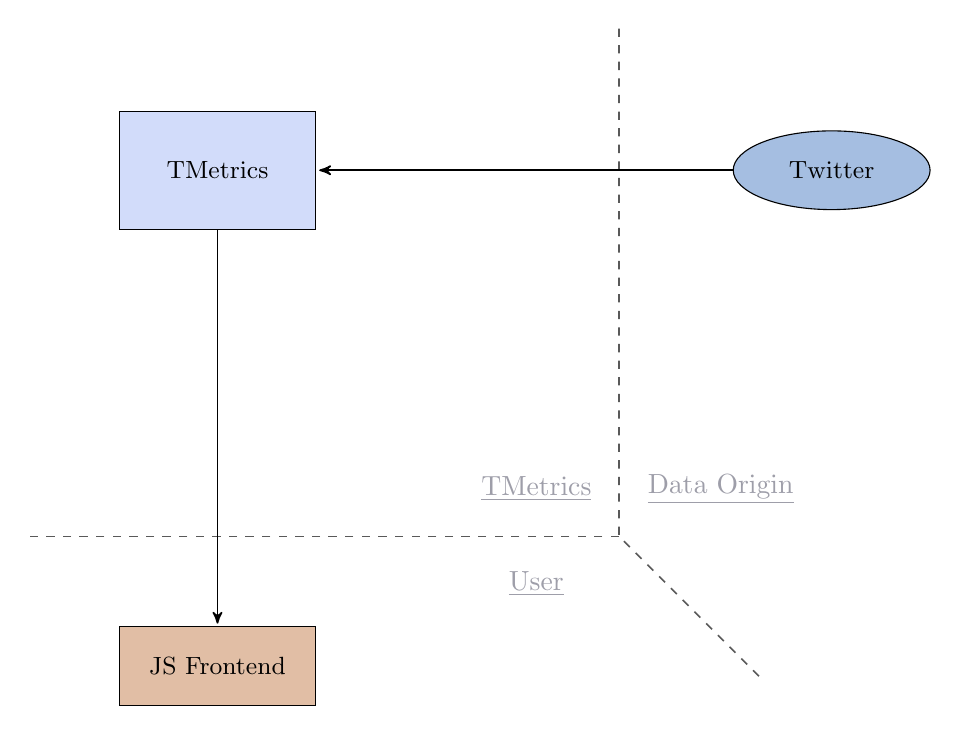
\begin{tikzpicture}[scale=.6,database/.style={
      cylinder,
      cylinder uses custom fill,
      cylinder body fill=lblue,
      cylinder end fill=lblue,
      shape border rotate=90,
      aspect=0.25,
      align=center,
      draw
    }]
    

\definecolor{silver}{RGB}{158,158,169}
\definecolor{midgray}{rgb}{.35,.35,.35}
\definecolor{lightsilver}{RGB}{221,221,232}
\definecolor{lblue}{RGB}{210,220,250}
\definecolor{mblue}{RGB}{165,190,225}
\definecolor{dblue}{RGB}{0,70,117}
\definecolor{lgreen}{RGB}{200,245,185}
\definecolor{mgreen}{RGB}{190,225,165}
\definecolor{mred}{RGB}{225,190,165}
\definecolor{dgreen}{RGB}{40,135,40}
\definecolor{dred}{RGB}{135,40,40}

\draw[-,dashed,semithick,midgray] (8.5,-7.75) -- (-4,-7.75);
\draw[-,dashed,semithick,midgray] (8.5,3) -- (8.5,-7.75) -- (11.5,-10.75);
\node[draw=none,silver] at (6.75,-6.75) {\underline{TMetrics}};
\node[draw=none,silver] at (10.65,-6.75) {\underline{Data Origin}};
\node[draw=none,silver] at (6.75,-8.75) {\underline{User}};

\node[fill=mred,draw=black,font=\small, minimum height=1cm, minimum width= 2.5cm] (fe) at (0, -10.5) {{JS Frontend}};
\node[ellipse,fill=mblue,draw=black,font=\small, minimum height=1cm, minimum width= 2.5cm] (tw) at (13, 0) {Twitter};

\node[fill=lblue,draw=black,minimum width=2.5cm, minimum height=1.5cm, font=\small] (tm) at (0,0) {TMetrics};
\draw[->,semithick,>=stealth',shorten >=1pt] (tw) -- (tm);
\draw[->,semithick,>=stealth',shorten >=1pt] (tm) -- (fe);


\end{tikzpicture}
}
\caption{Grundstruktur}
\label{arch1}
\end{figure}

\section{Beschaffung der Daten}

Recherchen zu Projektbeginn haben gezeigt, dass die grundsätzliche Möglichkeit zum Zugriff auf Tweets, Benutzerinformationen und sonstige Daten über die Twitter-API besteht. Diese Möglichkeit ist allerdings auch mit einer Reihe von Einschränkungen verbunden. Diese ermöglichen nur den Zugriff auf Tweets der letzten Tage und begrenzen außerdem die Anzahl der Tweets, welche innerhalb eines spezifischen Zeitraums zurückgeliefert werden können. Das macht es notwendig, dass TMetrics die benötigten Daten in regelmäßigen Abständen von Twitter abruft und in einer eigenen Datenbank speichert. Dies geschieht durch einen kontinuierlich laufenden Prozess, welcher von uns als Daemon bezeichnet wird. Da die Gesamtheit aller auf Twitter verfügbaren Daten unsere verfügbaren Kapazitäten überschreiten würde, haben wir uns dafür entschieden, auf diese Weise nur jene Daten zu sammeln, welche mit bereits eingegebenen Suchbegriffen in Verbindung stehen. Für diese Suchbegriffe war allerdings der Anspruch, sämtliche verfügbaren Daten zu sammeln, selbst wenn dafür zunächst noch keine Darstellung im Frontend vorgesehen war. Aus diesem Grund orientiert sich das Datenbankschema an den von Twitter zur Verfügung stehenden Daten. Um diese Entscheidungen zu realisieren, war eine Auswahl von Technologien erforderlich. 

Bei der Wahl der Datenbank bestand Einigkeit über den Einsatz eines relationalen Datenbanksystems. Außerdem sollte ein System gewählt werden, mit dem alle Projektmitglieder Erfahrung hatten, da die Datenbank als zentraler Bestandteil der Projektarchitektur erkannt wurde, mit der viele Programmbestandteile interagieren müssen. Aus diesen Gründen fiel die Wahl auf MySQL, das sämtlichen Projektmitgliedern bekannt war. Des Weiteren gab es unter uns keinen Datenbankexperten, der eine besser geeignete Datenbank hätte vorschlagen können. Da das Datenbanksystem vor Projektbeginn nicht als wichtige Technologie erkannt wurde, bestand keine Zeit mehr für Recherchen zu Alternativen, da die dadurch entstandene Verzögerung wegen der zentralen Rolle der Datenbank den gesamten Projektfortschritt verzögert hätte. Da der Daemon in Java implementiert wurde und auf die Datenbank zugreifen sollte, war der Einsatz einer geeigneten Bibliothek als Schnittstelle notwendig. Aufgrund bestehender Erfahrungen fiel die Wahl dabei auf JDBC \cite{JDBC}.

Neben einer Schnittstelle zur Datenbank war ebenfalls eine Schnittstelle zu Twitter notwendig, um die zu speichernden Daten überhaupt erst zu erhalten. Die bereits erwähnte API funktioniert dabei nach dem REST-Prinzip (siehe Abschnitt \ref{resteinfuehrung}). Das bedeutet, dass der Zugriff auf bestimmte Arten von Daten mit einer bestimmten URL (Ressource) verbunden ist. So stellen beispielsweise die Tweets eine Ressource von Twitter dar, auf die dann mittels eines HTML-GET-Requests auf die entsprechende URL in Verbindung mit geeigneten Parametern (z.\,B. ein in dem Tweet vorkommender Suchbegriff oder Hashtag) zugegriffen werden kann. Die Antwort wird dann im JSON-Format zurückgeliefert. Allerdings ist diese API nicht öffentlich zugänglich, sondern erfordert einen Twitter-Account. Über diesen kann dann über das OAuth-Authentifizierungsprotokoll eine Reihe von Tokens erstellt werden, welche bei der REST-Anfrage übergeben werden müssen, um eine Antwort zu erhalten. Um diese Schwierigkeit zu umgehen, aber auch um die Kommunikation mit der REST-API allgemein sicherer und einfacher zu gestalten, wurde auch für diese Schnittstelle nach einer Java-Bibliothek gesucht. Dabei fiel die Wahl auf Twitter4J. In dieser Bibliothek ist es möglich, durch einmalige Angabe der benötigten Tokens eine Verbindung mit Twitter herzustellen. Über diese Verbindung können dann REST-Anfragen gestellt werden, wobei dedizierte Methoden die sichere Übergabe der benötigten Parameter ermöglichen. Sämtliche Anfragen sind dann damit automatisch authentifiziert. Zu Beginn wurde zu Testzwecken zunächst ein Twitter-Account angelegt. Im Verlauf des Projekts waren allerdings aufgrund von Beschränkungen des Zugriffsvolumens weitere Accounts notwendig. Ein genauerer Überblick über diese Beschränkungen allgemein sowie die daraus resultierende Funktionsweise des Daemon wird im weiteren Verlauf dieser Arbeit im Abschnitt der Daemon-Komponente (siehe Abschnitt \ref{sec:daemon}) geliefert.

\section{Darstellung der Daten}
\label{sec:architekturDarstellung}

Wie bereits erwähnt, sollen die gesammelten Daten auf Anfrage des Benutzers im Frontend (unter Umständen nach Abschluss zusätzlicher Analysen) dargestellt werden. Das Design des Frontends wird ausführlich im Abschnitt der entsprechenden Komponente beschrieben (siehe Kapitel \ref{sec:frontend}). Die grundsätzliche Idee war jedoch, sich an der Gestalt von Suchmaschinen zu orientieren. Das Element der zusätzlichen Analyse und Aufbereitung der vorhandenen Daten legt außerdem einen Vergleich zu Seiten wie Wolfram Alpha nahe. Das bedeutet, dass der Benutzer zu Beginn einen Suchbegriff eingibt, der in den zu untersuchenden Tweets vorkommen soll. Damit der Daemon nach bereits angefragten Begriffen suchen kann, werden diese in der Datenbank in eine Tabelle eingetragen. Hat der Daemon zu dem Begriff bereits Daten gesammelt, können diese zur Darstellung zurückgeliefert werden. Dabei gibt es eine Reihe unterschiedlicher Gesichtspunkte, nach denen die vorhandenen Daten dargestellt werden können, beispielsweise das aktuelle Meinungsbild, die Aktivität zu dem Suchbegriff im zeitlichen Verlauf oder das Clustering. Die Ergebnisse zu jedem dieser Gesichtpunkte werden in einer entsprechenden Box, der sogenannten Ansicht, dargestellt. Dabei benötigt jede Ansicht eine entsprechende Auswahl der Daten aus der Datenbank sowie unter Umständen die Ergebnisse von deren Analyse. Damit ist klar, dass eine Schnittstelle notwendig ist, welche es ermöglicht, von Client-Seite Informationen in die Server-Datenbank einzutragen (vor allem zum Hinzufügen neuer Suchbegriffe) und außerdem gemäß bestimmten Anfragen Daten aus der Server-Datenbank an den Client zu senden. Die Entscheidung fiel daher darauf, aufgrund von bereits bestehenden Erfahrungen von Projektmitgliedern sowie in Anlehnung an die bekannte Twitter-API einen REST-Service zu erstellen. Dieser wurde wie im Abschnitt der REST-Komponente (siehe Kapitel \ref{sec:rest}) näher beschrieben mithilfe der JAX-RS-Bibliothek Jersey als Tomcat-Servlet implementiert. Diese ermöglicht es, Ressourcen mit Java-Methoden zu verknüpfen, welche bei Aufruf der mit der Ressource verbundenen URL ausgeführt werden. Dabei wurde jede Ansicht mit einer Ressource verknüpft, welche die für die Ansicht benötigten Daten durch Aufruf einer GET-Anfrage zurückliefert. Die damit verknüpfte Methode beinhaltet dabei immer einen Zugriff auf die Datenbank über JDBC mittels einer geeigneten SQL-Anfrage. Informationen, welche die Anfrage einschränken, werden dabei als Parameter an die Anfrage angehängt und entsprechend in den SQL-Befehl eingefügt. Das Einfügen von Daten in die Datenbank geschieht analog über POST-Anfragen. Bei manchen Anfragen ist außerdem noch eine zusätzliche Analyse oder Aufbereitung der Daten notwendig, was im folgenden Abschnitt beschrieben wird. Diese finden nach Zugriff auf die Datenbank, jedoch vor Senden der Antwort an den Client durch das Jersey-Servlet statt. Als Format für die Antwort des REST-Services haben wir JSON gewählt, da es einen einfachen Zugriff durch JavaScript ermöglicht.

Die Notwendigkeiten zur Beschaffung und Darstellung der Daten liefert ein grundlegendes Architekturmodell von TMetrics bestehend aus Daemon und REST-Service, welches in Abbildung \ref{arch2} dargestellt ist.

\begin{figure}[h]
\centering
\scalebox{0.7}{
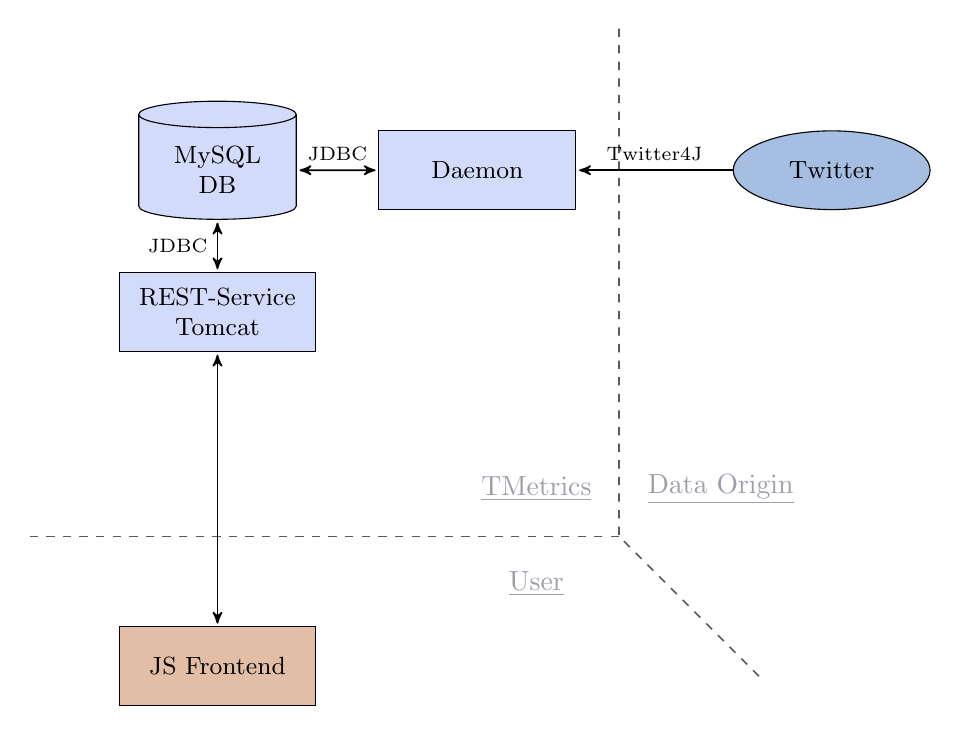
\begin{tikzpicture}[scale=.6,database/.style={
      cylinder,
      cylinder uses custom fill,
      cylinder body fill=lblue,
      cylinder end fill=lblue,
      shape border rotate=90,
      aspect=0.25,
      align=center,
      draw
    }]
    

\definecolor{silver}{RGB}{158,158,169}
\definecolor{midgray}{rgb}{.35,.35,.35}
\definecolor{lightsilver}{RGB}{221,221,232}
\definecolor{lblue}{RGB}{210,220,250}
\definecolor{mblue}{RGB}{165,190,225}
\definecolor{dblue}{RGB}{0,70,117}
\definecolor{lgreen}{RGB}{200,245,185}
\definecolor{mgreen}{RGB}{190,225,165}
\definecolor{mred}{RGB}{225,190,165}
\definecolor{dgreen}{RGB}{40,135,40}
\definecolor{dred}{RGB}{135,40,40}

\draw[-,dashed,semithick,midgray] (8.5,-7.75) -- (-4,-7.75);
\draw[-,dashed,semithick,midgray] (8.5,3) -- (8.5,-7.75) -- (11.5,-10.75);
\node[draw=none,silver] at (6.75,-6.75) {\underline{TMetrics}};
\node[draw=none,silver] at (10.65,-6.75) {\underline{Data Origin}};
\node[draw=none,silver] at (6.75,-8.75) {\underline{User}};


\node[fill=mred,draw=black,font=\small, minimum height=1cm, minimum width= 2.5cm] (fe) at (0, -10.5) {{JS Frontend}};
\node[ellipse,fill=mblue,draw=black,font=\small, minimum height=1cm, minimum width= 2.5cm] (tw) at (13, 0) {Twitter};


\node[database, minimum width=2cm, minimum height=1.5cm, font=\small] (db) at (0,0) { MySQL \\ DB}; %
\node[fill=lblue,draw=black,font=\small, minimum height=1cm, minimum width= 2.5cm,align=center] (rs) at (0, -3) {REST-Service \\ Tomcat}; %
\node[fill=lblue,draw=black,font=\small, minimum height=1cm, minimum width= 2.5cm] (de) at (5.5, 0) {Daemon};

\draw[->,semithick,>=stealth',shorten >=1pt] (tw) -- (de) node[midway,above,font=\scriptsize] {Twitter4J};
\draw[<->,semithick,>=stealth',shorten >=1pt,shorten <=1pt] (de) -- (db) node[midway,above,font=\scriptsize] {JDBC};
\draw[<->,semithick,>=stealth',shorten >=1pt,shorten <=1pt] (db) -- (rs) node[midway,left,font=\scriptsize] {JDBC};

\draw[<->,semithick,>=stealth',shorten <=1pt,shorten >=1pt] (rs) -- (fe);


\end{tikzpicture}
}
\caption{Grundlegendes Architekturmodell}
\label{arch2}
\end{figure}

\section{Analyse der Daten}

Aus den beiden Hauptanwendungsbereichen Beschaffung der Daten von Twitter und Ausgabe der Daten an das Frontend ergibt sich die Projektstruktur von TMetrics: einerseits existiert ein REST-Service als Tomcat-Servlet auf dem Server, welcher auf Benutzeranfragen reagiert, und andererseits gibt es den Daemon, welcher kontinuierlich als gewöhnliche Java-Anwendung auf dem Server läuft. Dieser ursprünglichen Vorstellung nach bildet die MySQL-Datenbank die einzige Schnittstelle zwischen diesen beiden Bestandteilen. Damit waren zu Projektbeginn zwei grundsätzlich unabhängige Programme vorgesehen, welche an unterschiedlichen Stellen des Servers ausgeführt werden sollten. Aus diesem Grund wurden zwei separate Java-Projekte erstellt, welche im Folgenden Daemon und REST-Service genannt werden. Allerdings übersteigt der ursprüngliche Funktionsumfang von TMetrics die bisher vorgestellten Aufgabenbereiche dieser Bestandteile, welche sich jeweils nur auf das Auslesen und Speichern der Daten von Twitter und der Ausgabe dieser Daten an das Frontend beschränken. Hinzu kommt nämlich noch die Zielsetzung, dass die gesammelten Daten außerdem auf verschiedene Weisen analysiert werden sollen. Dies wirft die Frage auf, in welchem der Bestandteile diese Analyse stattfinden soll. Eine Durchführung im Daemon bedeutet dabei, dass die Analyse bereits bei Erhalt sämtlicher Daten durchgeführt wird und ihre Ergebnisse in der Datenbank persistent gehalten werden müssen. Im Gegensatz dazu wird eine Analyse im REST-Service nur durchgeführt, wenn eine entsprechende Anfrage des Benutzers gestellt wird. Das Speichern der dabei bestimmten Ergebnisse in der Datenbank ist möglich, aber nicht zwingend notwendig. Dabei muss in Betracht gezogen werden, wie häufig die Ergebnisse benötigt werden und wie schnell sie durch vom Daemon neu hinzugefügte Daten veralten können. Da das Sentiment eines Tweets nur von seinem Text abhängt, ist die Sentiment-Analyse nicht von neu hinzukommenden Tweets abhängig, muss daher nicht aktualisiert werden und kann daher direkt beim Hinzufügen des Tweets durch den Daemon durchgeführt werden (es ist möglich, dass das Sentiment aktualisiert werden muss, falls sich das zu Grunde liegende Modell ändert, was jedoch vergleichsweise selten vorkommt. Details dazu im Abschnitt der Sentiment-Analyse, Kapitel \ref{sec:Sentiment}). Des Weiteren sind zur Erstellung des aktuellen Meinungsbildes eines Suchbegriffs ohnehin die Sentiment-Werte sämtlicher Tweets mit diesem Suchbegriff notwendig. Die Cluster-Analyse sowie die Bestimmung von Peaks und zugehörigen News in der Aktivitätskurve sind hingegen von sämtlichen Tweets in der Datenbank abhängig. Daher müssten die Ergebnisse dieser Verfahren ständig aktualisiert werden, sobald neue Tweets eines Suchbegriffs der Datenbank hinzugefügt werden. Da dies weitaus häufiger vorkommt als eine Anfrage an den Begriff, finden diese beiden Analysemethoden im REST-Service statt. Die Ergebnisse werden auf der Serverseite nach ihrem Abschicken an den Client nicht weiter gespeichert.

Einen Sonderfall bildet hierbei die Sentiment-Analyse. Nachdem im Projektverlauf mehr Gewicht auf den Aspekt des explorativen Arbeitens auf den zurückgelieferten Daten gelegt wurde, ist es nun auch wünschenswert, dass im Frontend angezeigt werden kann, welche Einflussfaktoren das Sentiment eines Tweets bestimmen und aus welchen Trainingsdaten diese Einflussfaktoren hervorgehen. Diese zusätzlichen Informationen gehen aus dem Sentiment-Modell hervor, welches wie zuvor beschrieben Teil des Daemon-Projekts ist. Zur Anzeige im Frontend müssen sie nun allerdings auch im REST-Service verfügbar sein. Eine Erweiterung der Datenbank um diese Einflussfaktoren wurde aufgrund des erhöhten Speicherbedarfs sowie der notwendigen Änderungen an der Datenbank mit Hinblick auf den Projektstand nicht vorgenommen. Stattdessen wurde entschieden, dass für Tweets, für die die Einflussfaktoren abgerufen werden, das Sentiment noch einmal erneut im REST-Service bestimmt wird. Der dadurch entstehende Zusatzaufwand ist hinnehmbar, da davon auszugehen ist, dass dies nur für einen Bruchteil der Tweets in der Datenbank durchgeführt wird. Damit ist allerdings der Einsatz der Klassen des Sentiment-Modells im REST-Service notwendig, sodass keine strikte Trennung beider Projekte mehr gegeben ist. Die Integration der Analysemethoden in das Architekturmodell ist in Abbildung \ref{arch3} zu sehen.

\begin{figure}[h]
\centering
\scalebox{0.7}{
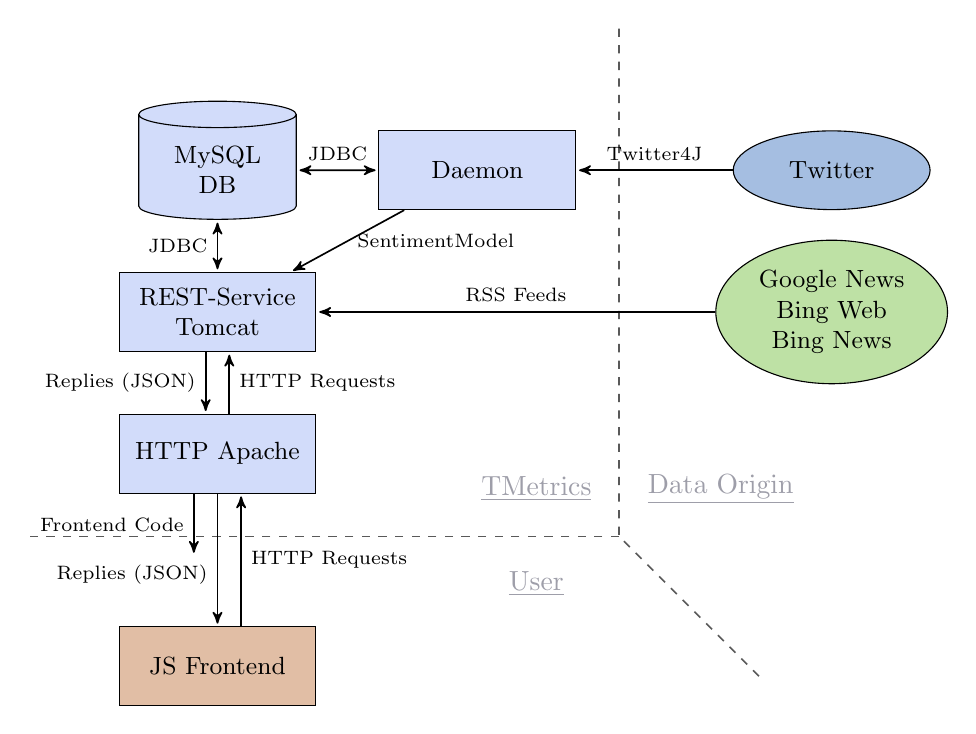
\begin{tikzpicture}[scale=.6,database/.style={
      cylinder,
      cylinder uses custom fill,
      cylinder body fill=lblue,
      cylinder end fill=lblue,
      shape border rotate=90,
      aspect=0.25,
      align=center,
      draw
    }]
    

\definecolor{silver}{RGB}{158,158,169}
\definecolor{midgray}{rgb}{.35,.35,.35}
\definecolor{lightsilver}{RGB}{221,221,232}
\definecolor{lblue}{RGB}{210,220,250}
\definecolor{mblue}{RGB}{165,190,225}
\definecolor{dblue}{RGB}{0,70,117}
\definecolor{lgreen}{RGB}{200,245,185}
\definecolor{mgreen}{RGB}{190,225,165}
\definecolor{mred}{RGB}{225,190,165}
\definecolor{dgreen}{RGB}{40,135,40}
\definecolor{dred}{RGB}{135,40,40}

\draw[-,dashed,semithick,midgray] (8.5,-7.75) -- (-4,-7.75);
\draw[-,dashed,semithick,midgray] (8.5,3) -- (8.5,-7.75) -- (11.5,-10.75);
\node[draw=none,silver] at (6.75,-6.75) {\underline{TMetrics}};
\node[draw=none,silver] at (10.65,-6.75) {\underline{Data Origin}};
\node[draw=none,silver] at (6.75,-8.75) {\underline{User}};

\node[fill=mred,draw=black,font=\small, minimum height=1cm, minimum width= 2.5cm] (fe) at (0, -10.5) {{JS Frontend}};
\node[ellipse,fill=mblue,draw=black,font=\small, minimum height=1cm, minimum width= 2.5cm] (tw) at (13, 0) {Twitter};

\node[database, minimum width=2cm, minimum height=1.5cm, font=\small] (db) at (0,0) { MySQL \\ DB}; %
\node[fill=lblue,draw=black,font=\small, minimum height=1cm, minimum width= 2.5cm,align=center] (rs) at (0, -3) {REST-Service \\ Tomcat}; %
\node[fill=lblue,draw=black,font=\small, minimum height=1cm, minimum width= 2.5cm] (de) at (5.5, 0) {Daemon};

\draw[->,semithick,>=stealth',shorten >=1pt] (tw) -- (de) node[midway,above,font=\scriptsize] {Twitter4J};
\draw[<->,semithick,>=stealth',shorten >=1pt,shorten <=1pt] (de) -- (db) node[midway,above,font=\scriptsize] {JDBC};
\draw[<->,semithick,>=stealth',shorten >=1pt,shorten <=1pt] (db) -- (rs) node[midway,left,font=\scriptsize] {JDBC};

\node[fill=lblue,draw=black,font=\small, minimum height=1cm, minimum width= 2.5cm,align=center] (ap) at (0, -6) {HTTP Apache};

\draw[->,semithick,>=stealth',shorten >=1pt] ([xshift=-0.5cm]ap.south) -- ([xshift=-0.5cm,yshift=1.5cm]fe.north) node[midway,left,align=right,font=\scriptsize] {Frontend Code};
\draw[<-,semithick,>=stealth',shorten <=1pt] ([xshift=0.5cm]ap.south) -- ([xshift=0.5cm]fe.north) node[midway,right,align=left,font=\scriptsize] {HTTP Requests};
\draw[->,semithick,>=stealth',shorten >=1pt] ([xshift=-0.25cm]rs.south) -- ([xshift=-0.25cm]ap.north) node[midway,left,font=\scriptsize] {Replies (JSON)};
\draw[<-,semithick,>=stealth',shorten <=1pt] ([xshift=0.25cm]rs.south) -- ([xshift=0.25cm]ap.north) node[midway,right,align=left,font=\scriptsize] {HTTP Requests};
\draw[->,semithick,>=stealth',shorten >=1pt] ([xshift=0cm]ap.south) -- ([xshift=0cm]fe.north) node[midway,left,align=right,font=\scriptsize] {\ \\ \ \\ Replies (JSON)};

\draw[<-,semithick,>=stealth',shorten <=1pt] (rs) -- (de) node[midway,right,font=\scriptsize] {SentimentModel};

\node[ellipse,fill=mgreen,draw=black,align=center,font=\small, minimum height=1cm, minimum width= 2.5cm] (ne) at (13, -3) {Google News \\ Bing Web \\ Bing News};
\draw[<-,semithick,>=stealth',shorten <=1pt] (rs) -- (ne) node[midway,above,font=\scriptsize] {RSS Feeds};


\end{tikzpicture}
}
\caption{Architekturmodell mit Analysemethoden}
\label{arch3}
\end{figure}

\chapter{Infrastruktur}
\label{cha:infrastruktur}
\section{Daemon}
\label{sec:daemon}
%\subsection{Motivation} % Jens
Wie schon erwähnt, ist eines unserer Ziele, Tweets von Twitter zu bestimmten Suchbegriffen, bei uns \textit{search terms} genannt, zu sammeln und weiterzuverarbeiten.
Da wir aufgrund einiger Restriktionen durch Twitter nicht direkt alle Tweets zu einem Thema bekommen können, ist es notwendig sie zwischenzuspeichern.
Der Service, der die Tweets von Twitter abruft und in der lokalen Datenbank speichert, wurde in Anlehnung an Unix-Dienste 
%(siehe dazu \url{https://de.wikipedia.org/wiki/Daemon}) 
Daemon genannt. 
Im folgenden Kapitel \ref{sssection:twitter-api} wird auf die Twitter-API sowie  die damit verbundenen Restriktionen eingegangen.
Anschließend wird in Abschnitt \ref{ssection:Suchstrategie} erklärt, wie die Tweets von Twitter abrufen  werden und insbesondere welche Suchstrategie dabei angewendet wird, um möglichst alle Tweets zu einem Thema zu finden.
Es folgt in Abschnitt \ref{ssection:parallele-suche} eine Beschreibung der Erweiterung der Suche zur parallelen Suche, um den Durchsatz der gefundenen Tweets zu erhöhen.
In diesem Rahmen wird auch das mit der Suche eingeführte Multi-Threading erläutert.
Als letzte Verbesserung des Daemon folgt in Abschnitt \ref{ssection:ZeitnaheErgebnisse} die Erläuterung wie möglichst zeitnah nach Eingabe eines neuen Suchbegriffs Ergebnisse erhalten werden.
Als letztes folgt im Abschnitt \ref{ssection:ausblick} eine Diskussion über 
weitere mögliche Erweiterungen der Fähigkeiten des Daemon, die nicht mehr umgesetzt werden konnten.
Das Sentiment wird zwar im Daemon berechnet, wird aber nicht hier beschrieben, sondern in Kapitel \ref{sec:Sentiment}, welches speziell nur das Thema Sentiment behandelt.

\subsection{Twitter-API}
\label{sssection:twitter-api}
Die Twitter-API umfasst alle Möglichkeiten über die zum Teil unterschiedlichen offiziellen Schnittstellen mit Twitter zu interagieren.
Sie bildet alle Funktionen ab, die notwendig sind, um einen Twitter-Client zu bauen.
Um die API verwenden zu können, benötigt man sowohl ein sogenanntes Profil, d.\,h. einen Account bei Twitter, als auch einen API-Key, den man selbst erzeugen kann.
Twitter unterscheidet zwischen dem sogenannten \textit{consumer key}, der an das Profil gebunden ist, und dem \textit{application key}, der an die Anwendung gebunden ist.
Dabei kann ein Nutzer verschiedene Apps nutzen, die alle einen eigenen \textit{application key} nutzen, sein \textit{consumer key} ändert sich aber nicht.
Genauso kann ein Entwickler mehrere Apps entwickeln, die alle einen unterschiedlichen \textit{application key} besitzen, sein \textit{consumer key} bleibt aber gleich.
Ein Nutzer muss bei einer App allerdings nicht selbst diese Keys eintragen, vielmehr fordert die App, die den \textit{application key} im Code enthält, den User auf, die App bei Twitter zu autorisieren.
Die Details lassen sich in der Twitter-Dokumentation, Abschnitt "`Access Token"' \cite{TwitterAccessTokens2014} entnehmen.
Das Authentifizierungssystem für Apps von Twitter basiert dabei auf  OAuth, auch hier finden sich wieder die Details in der Twitter-Dokumentation \cite{TwitterOAuth2014}.
Unser Daemon greift im Gegensatz dazu etwas anders auf Twitter zu.
So haben wir für jedes genutzte Profil eine eigene App bei Twitter registriert und die jeweiligen \textit{consumer} und \textit{application Keys} direkt verwendet.
Diese Art des Zugriffs ist eigentlich nur für Entwickler vorgesehen.

\subsubsection{Beschränkungen der Twitter-API}
Grundsätzlich bietet Twitter zwei unterschiedliche APIs: die REST-API und die Streaming-API. Bei der REST-API müssen explizite Anfragen gestellt  werden, um Daten zu erhalten, während bei der Streaming-API zu gewissen Themen oder Usern ständig die aktuellen Daten übermittelt werden, solange man eine Verbindung offen hält.
Die einzige für uns relevante Funktionalität ist die Suche nach den durch den Nutzer vorgegeben Begriffen, deswegen beschränken wir uns auf die Funktionalität zum Suchen nach Tweets.
Das ist grundsätzlich mit beiden APIs möglich, die Streaming-API würde es uns aber nur erlauben, Tweets zu dem gesuchten Begriff zu erhalten, die nach unserer Anfrage erstellt wurden. Das folgt aus der zweiten Grafik in der Dokumentation der Twitter Streaming-API \cite{TwitterStreamingAPIs2014}.
Es ist mit der Streaming-API also nicht möglich Tweets zu finden, die zeitlich vor Beginn unserer Anfrage erstellt wurden.
Die REST-API hingegen erlaubt es uns auch nach Tweets zu suchen, die schon vor Beginn unserer Anfrage erstellt wurden.
Allerdings gibt es auch hier  Beschränkungen.
So garantiert Twitter nicht, dass man Tweets findet, die älter als ca. 6-9 Tage sind, obwohl es durchaus ältere Tweets geben kann.
Die Dokumentation zur Nutzung der Suche \cite{TwitterUsingSearch2014} sagt dazu 
\begin{quote}
The Search API is not a complete index of all Tweets, but instead an index of recent Tweets. At the moment that index includes between 6-9 days of Tweets.
\end{quote}
Ebenfalls hier wird auch die Beschränkung erläutert, dass Twitter keine Vollständigkeit der Ergebnisse garantiert, sondern nur davon spricht, die möglichst relevanten Ergebnisse zu liefern.
Weitere Beschränkungen sind:
\begin{itemize}
\item maximal 100 Tweets pro Anfrage und
\item maximal 180 Anfragen pro 15-Minuten-Intervall pro Account (siehe \textit{REST API v1.1 Limits per window by resource} in der Twitter Dokumentation \cite{TwitterRESTLimitsperResource2014}).
\end{itemize}
Eine Einführung in diese \textit{rate limits} genannten Beschränkungen findet sich im Artikel \textit{REST API Limiting in v1.1} (\cite{TwitterRESTAPIv1.1}) der offiziellen Dokumentation.
Für uns ist außerdem noch relevant, dass Twitter es nicht ermöglicht die Suche durch kleinere Intervalle als Tage einzuschränken.
Dafür ist es möglich die Suche durch Angabe einer maximalen bzw. minimalen Tweet-ID einzuschränken.
Diese sowie weitere mögliche Parameter bei der Suche sind im \textit{GET search/tweets} Artikel \cite{TwitterSearch2014} der Twitter-Dokumentation zu finden.
Ebenfalls hier werden die \textit{result types} eingeführt.
Die \textit{result types} geben dabei an, von welcher Art das Ergebnis ist. Mögliche Werte sind:
\begin{itemize}
\item \texttt{popular} - Enthält nur die populärsten Tweets 
\item \texttt{recent} - Enthält die aktuellsten Tweets
\item \texttt{mixed} - Enthält beide Arten von Tweets
\end{itemize}
Dabei liefert der \textit{result type} \texttt{recent} nicht nur aktuelle Tweets, sondern diese auch in einer chronologischen Sortierung.
Wir konnten in eigenen Tests keine nicht-chronologische Abfolge von Tweets feststellen.
Außerdem scheint \texttt{recent} es uns zu erlauben alle Tweets zu erhalten, die Twitter uns zur Verfügung stellt.
Wir konnten jedenfalls keine fehlenden Tweets feststellen, als wir mit den verschiedenen Strategien experimentiert haben. %TODO: Beim Vergleich mit der Websiuche von Twitter
Unsere Tests erfolgten dabei unter der Annahme, dass die mit \texttt{recent} erhaltenen Tweets streng chronologisch sind.
Leider waren wir nicht in der Lage, eine genaue Aussage zur Chronologie und Vollständigkeit der verschiedenen \textit{result types} in der Twitter-Dokumentation zu finden.

\subsection{Suchstrategie} % torsten
\label{ssection:Suchstrategie}

Um Tweets von Twitter systematisch abzufragen, wird eine intelligente Suchstrategie benötigt.
Die Strategie muss sich dabei den durch Twitter auferlegten Einschränkungen anpassen.
Beispielsweise ist es mit der Search-API, die Teil der bereits erwähnten REST-API ist und für die Suche nach Tweets verwendet wird, nicht möglich, nach Tweets in Zeiträumen von Stunden oder Minuten zu suchen.
Stattdessen bietet Twitter mit der Search-API die Suche nach Tweets in Zeitintervallen von Tagen oder die Suche bis zu einer Tweet-ID an.
Letzteres bedeutet, dass eine Anfrage zu einem Suchbegriff an Twitter mit einer Tweet-ID gesendet werden kann, in der der Benutzer die 100 letzten Tweets zu diesem Suchbegriff mit einer ID kleiner als der in der Anfrage verwendeten ID erhält.

Im Daemon gab es zwei Ansätze, wie die Suche durchzuführen sein sollte.
Der erste Ansatz sah vor, dass in der ersten Phase ab dem Zeitpunkt $t$, an dem ein neuer Suchbegriff in die Datenbank geschrieben wurde, bei Twitter nach Tweets gesucht wird, die vor $t$ veröffentlicht wurden.
Werden anschließend keine neuen Tweets mehr gefunden, deren Erstelldatum vor $t$ liegt, so wird nun in einer zweiten Phase ab $t$ nach neuen Tweets gesucht.
Abbildung \ref{fig:search_1} verdeutlicht diesen Ansatz.

\begin{figure}
\centering
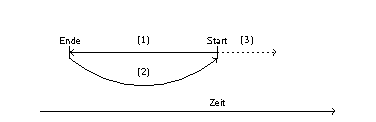
\includegraphics[width=\textwidth]{Bilder/Daemon/SearchStrategy1.pdf}
\caption{Der erste Ansatz. Zunächst wird vom Start aus rückwärts gesucht (1). Anschließend wird wieder zum ursprünglichen Start gesprungen (2). Von dort aus wird dann vorwärts nach neuen Tweets gesucht (3).\label{fig:search_1}}
\end{figure}

Der alternative Ansatz unterscheidet sich in der zweiten Phase vom ersten Ansatz.
Anstatt ab Zeitpunkt $t$ in Richtung Gegenwart zu suchen, wird der Zeitpunkt $t$ auf "`jetzt"' neu gesetzt.
Anschließend wird wieder nach Tweets gesucht, die vor dem neuen $t$ veröffentlicht worden sind, bis anschließend keine neuen Tweets mehr gefunden werden.
Dann wird $t$ erneut gesetzt und die Suche beginnt abermals.
Dieser Ansatz besteht also aus vielen, aneinandergereihten Einzelsuchen.
In Abbildung \ref{fig:search_2} wird der zweite Ansatz skizziert.

\begin{figure}
\centering
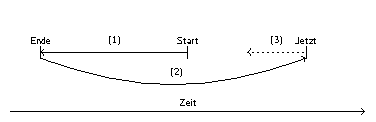
\includegraphics[width=\textwidth]{Bilder/Daemon/SearchStrategy2.pdf}
\caption{Der alternative Ansatz. Zunächst wird vom Start aus rückwärts gesucht (1). Anschließend wird zum jetzigen Zeitpunkt gesprungen (2). Von dort aus wird wieder rückwärts gesucht (3).\label{fig:search_2}}
\end{figure}

Wir haben uns für den zweiten Ansatz entschieden, da sich dieser gut mit den Einschränkungen durch Twitter verträgt und keine Phasen unterscheiden muss, wie es im ersten Ansatz der Fall ist.
Aus diesem Grund wurde auch auf die Verwendung der Streaming-API verzichtet, da der Daemon stets rückwärts sucht und nicht über gerade neu veröffentlichte Tweets sofort informiert werden muss.

\subsubsection{Details der Suchstrategie}

Auch wenn die im Daemon implementierte Suchstrategie keine unterschiedlichen Phasen besitzt, so gibt es aber doch unterschiedliche Zustände, in denen sich die Suchlogik befinden kann.
Wie bereits erwähnt, besteht die Suche aus aneinandergereihten Einzelsuchen.
Diese Einzelsuchen haben wir \emph{Iterationen} genannt.
Eine Iteration kann sich in zwei Zuständen befinden.
Hat sie noch nicht begonnen, dann wurde noch nicht nach neuen Tweets, die vor dem Zeitpunkt $t$ veröffentlicht worden sind, gesucht.
In der Iteration kann jedoch auch schon nach neuen Tweets gesucht worden sein, deren Erstelldatum vor $t$ liegt.
In diesem Fall ist die Iteration \emph{aktiv}. 

Bevor auf genaue Details der Suchlogik eingegangen werden kann, muss zunächst der Begriff der \emph{Intervalllänge} erläutert werden.
Die Intervalllänge ist ein Zeitraum, der mit einem Suchbegriff assoziiert ist.
Dieser Zeitraum bestimmt, wann erneut nach diesem Suchbegriff gesucht werden soll.
Denn nach Begriffen, die wenig Aktivität erfahren, es also über einen längeren Zeitraum nur wenige neue Tweets gibt, sollte weniger häufig gesucht werden als nach Begriffen, die eine starke Aktivität besitzen, es also permanent viele neue Tweets gibt.
Dies ist insbesondere deswegen sinnvoll, weil ein für die Suche verwendetes Twitter-Profil nur beschränkt viele Anfragen innerhalb von 15 Minuten zur Verfügung hat.
Dieser Sachverhalt wird im Abschnitt über das \textit{scheduling} weiter vertieft werden.

Zu Beginn der Suche ist die Iteration nicht aktiv.
Der Suchzeiger, der angibt, wo wir uns auf dem Zeitstrahl der Iteration befinden, steht also auf dem Zeitpunkt $t$.
In diesem Fall muss die Intervalllänge des zu bearbeitenden Suchbegriffs betrachtet werden.
Ist der Zeitraum, der zwischen der letzten Suche und $t$ liegt, kleiner als die Intervalllänge, so darf nicht nach dem Suchbegriff gesucht werden.
Wir setzen in diesem Fall $t$ neu auf den jetzigen Zeitpunkt, sodass bei einem erneuten Prüfen, ob gesucht werden soll, die Möglichkeit besteht, dass die Intervalllänge nun überschritten worden ist.
In dem Fall wird dann einmal nach Tweets gesucht, deren Erstelldatum vor $t$ liegt.
Anschließend werden für die Suche nur noch Tweets-IDs verwendet, da Twitter keine Suche nach exakten Zeitpunkten zulässt.
Dazu werden Anfragen an Twitter gestellt, die neben dem Suchbegriff auch die Tweet-ID $id$ beinhalten.
Twitter liefert dann für den Suchbegriff bis zu 100 Tweets, deren IDs kleiner als $id$ sind.
Gleichzeitig sind diese Tweets chronologisch sortiert und liegen zeitlich direkt vor dem Erstellzeitpunkt des Tweets von $id$.
Aus diesen den erhaltenen Tweets wird anschließend der älteste ausgewählt, dessen ID als neuer Suchanker dient.
So hangelt sich der Suchzeiger anhand der Tweet-IDs zeitlich rückwärts entlang, bis keine neuen Tweets mehr gefunden werden.
In dem Fall wird $t$ neu gesetzt und die aktuelle Iteration beendet.
Insbesondere wird die Intervalllänge nicht beachtet, wenn die Iteration aktiv ist.

Ein kleines Beispiel verdeutlicht diesen Ablauf:
Wir befinden uns am Anfang der Iteration, sie ist also noch nicht aktiv.
In $t$ steht der momentane Zeitpunkt und die Intervalllänge wird überschritten.
Also darf gesucht werden.
Dazu wird für einen Suchbegriff eine Anfrage an Twitter gestellt, die 100 jüngsten Tweets vor dem jetzigen Zeitpunkt zu liefern.
Twitter ermöglicht zwar keine Suche zu bestimmten Zeitpunkten, bietet jedoch die Funktionalität, die 100 jüngsten Tweets vor dem aktuellen Zeitpunkt anzufordern.
Alle Tweets werden zwischengespeichert, jedoch noch nicht in der Datenbank abgespeichert (siehe dazu Abschnitt den Abschnitt über die Architektur des Daemons).
Aus diesen Tweets wählen wir den ältesten aus und merken uns seine Tweet-ID.
In einer nächsten Anfrage liefert uns Twitter die 100 jüngsten Tweets vor dem Tweet mit der gemerkten ID.
Auch hier wählen wir wieder den ältesten aus, den wir für eine neue Anfrage nutzen können.
Dies wird so lange fortgeführt, bis keine neuen Tweets mehr gefunden werden.
Das kann zwei Ursachen haben:
Zum einen kann es sein, dass die Iteration einen viel zu langen Zeitraum überstreckt (also mehr als 6-9 Tage).
Dann liefert Twitter grundsätzlich keine Tweets mehr aus.
Also muss die Iteration beendet werden.
Zum anderen kann es aber auch sein, dass das komplette Intervall abgearbeitet wurde und wir Tweets finden, deren Erstelldatum bereits vor dem Startzeitpunkt der vorhergegangen Iteration liegen.
Diese Tweets liegen schon bereits alle in der Datenbank, weswegen die Iteration beendet werden kann.

\subsubsection{Berechnung der Intervalllänge}

Die Intervalllänge gibt an, wann zu einem Suchbegriff gesucht werden soll.
Ist noch nicht genug Zeit seit dem letzten Iterations-Startzeitpunkt vergangen, so wird noch nicht nach dem Suchbegriff gesucht.
Denn ansonsten würde sehr häufig nach Suchbegriffen gesucht werden, zu denen es keine bis nur sehr wenige, neue Tweets gibt.
So würden unnötig viele Suchanfragen gestellt und die Twitter-Profile deswegen nicht optimal ausgenutzt werden.
Es erscheint daher sinnvoll, nur dann nach Suchbegriffen zu suchen, wenn davon ausgegangen werden kann, mit einer einzigen Suchanfrage alle neuen Tweets zu finden.
Da eine Anfrage höchstens 100 Tweets liefert, muss die Anzahl der mit einer Anfrage aufzufindenden Tweets also auf 100 gesetzt sein.
Nach einem Suchbegriff, zu dem in der Stunde im Schnitt nur zwei neue Tweets veröffentlicht werden, sollte also ungefähr alle 50 Stunden gesucht werden.
Falls der Benutzer jedoch zeitiger Ergebnisse sehen möchte, kann er die Intervalllänge über die Benutzer-Priorisierung für den Suchbegriff reduzieren.
Analog können nicht so wichtige Suchbegriffe über eine negative Priorisierung eine längere Intervalllänge erhalten.

Um festzustellen, wie häufig neue Tweets zu einem Suchbegriff vorkommen, wird während der gesamten Suche der jüngste und der älteste gefundene Tweet festgehalten (nicht der jüngste und älteste einer Anfrage).
Über die über den gesamten Zeitraum zwischen ältesten und jüngsten Tweet gefundenen, neuen Tweets lassen sich die Tweets pro Minute ($TPM$) ermitteln.
Anhand der $TPM$-Zahl lässt sich der Zeitraum bestimmen, über welchem erwartungsgemäß weitere 100 neue Tweets vorhanden sein werden.
Da die Anzahl der neuen Tweets aber immer etwas schwankt und nicht konstant gleich bleibt, gibt es noch einen Korrekturwert, der mit der Intervalllänge multipliziert wird.
Der Wert wurde auf $0,9$ festgelegt.
Veranschaulicht werden dann nur 90 der 100 neuen Tweets gefunden, da nur $90\%$ des Zeitraums abgedeckt werden.
Dieser Faktor soll sicherstellen, dass leichte Abweichungen nach oben nicht eine weitere Anfrage provozieren.
Stattdessen wird der Puffer von noch 10 Tweets verwendet.
Zukünftig wird die Intervalllänge anschließend gekürzt, da nicht so viel Zeit wie durch die Intervalllänge vorgegeben ist, vergehen muss.
Falls es hingegen eine Abweichung nach unten gibt, so wird die Intervalllänge verlängert werden, da mehr Zeit verstreichen muss, bis 90 Tweets gefunden werden.

Insgesamt ergibt sich die Intervalllänge $I$ gemäß folgender Formel:

$$I = p \cdot \frac{1}{TPM} \cdot t \cdot 100,$$

wobei $p \in \{\,0,5;\,0,75;\,1;\,1,5;\,2\,\}$ der Benutzer-Priorität von positiv ($0,5$ und $0,75$) über neutral ($1$) bis negativ ($1,5$ und $2$) entspricht, $TPM$ die Tweets pro Minute sind und $t$ dem \textit{throttle factor} von $0,9$ entspricht.
Die 100 entspricht den 100 angepeilten, neuen Tweets, die es über den Zeitraum der Intervalllänge zu finden gilt.

Für den Fall, dass kein oder nur 1 Tweet gefunden wurde, wird die momentane Intervalllänge mit einem "`Außenseiter"'-Faktor multipliziert, die aktuell auf 3 gesetzt ist.
Das Eintreten dieses Falls ist unerwartet, da die Intervalllänge ja auf 90 Tweets ausgelegt war.
Aus diesem Grund wird sie verlängert, da der Suchbegriff offenbar ein unerwartetes Ereignis durchlebt haben muss, was die Intervalllänge vorher hat falsche Annahmen machen lassen.
Die Intervalllänge kann insgesamt eine Länge von sechs Tagen erreichen, nicht jedoch mehr. Dieser Wert wurde gewählt, da Twitter Tweets nur bis zu sechs Tagen in die Vergangenheit garantiert.
Dies stellt zwar nicht sicher, dass alle Tweets in dem Zeitraum der letzten Tage gefunden werden (weil vielleicht eine plötzliche, unerwartete Aktivität mit dem Suchbegriff verbunden ist), aber ein noch längeres Warten wäre sinnlos, da dann tatsächlich Tweets verloren gehen würden.
Da die Zeit für das Erneuern des \textit{rate limits} durch Twitter auf 15 Minuten festgelegt ist, sollte die Intervalllänge mindestens eine Länge von 15 Minuten besitzen.
Aus diesem Grund wird eine Intervalllänge, die laut der Formel kürzer als 15 Minuten lang ist, automatisch auf 15 Minuten festgelegt.

\subsubsection{Scheduling}
Die Anzahl der Suchanfragen innerhalb von 15 Minuten ist durch Twitter beschränkt, weswegen die Anzahl der Suchanfragen zu einer effizient zu verwaltenen Ressource wird. Aus diesem Grund wurde im Daemon ein intelligentes Verhalten zur effizienten Verwaltung der Suchbegriffe eingefügt, um möglichst nur dann eine Suche zu einem Suchbegriff zu starten, wenn dies auch sinnvoll erscheint.

Die Grundidee ist es nun, dass der Daemon immer nur dann eine Anfrage zu einem Suchbegriff startet, wenn er die 100 neuen Tweets seit dem letzten Abrufen mit einer Anfrage sammeln kann. Dies ist eine signifikante Verbesserung der Auslastung von Suchbegriffen im Vergleich zum ursprünglichen Verhalten, bei dem der Daemon zu jedem aktiven Suchbegriff immer mindestens eine Anfrage bei Verwendung eines frischen Twitter-Profils.

Um ein intelligentes Scheduling-Verhalten der Suchgriffe zu gewährleisten, werden Suchbegriffe in zwei Klassen unterteilt: \textit{short search terms} und \textit{long search terms} (auch einfach nur \textit{short terms} und \textit{long terms}).

Unter \textit{short terms} verstehen wir solche Suchbegriffe, die eine Intervalllänge \emph{länger} als die minimale, durch Twitter vorgegebene \textit{rate limit} Resetzeit besitzen, was zur Zeit 15 Minuten sind. Das bedeutet, dass zu diesem Suchbegriff idealerweise innerhalb von einer Anfrage alle neuen Tweets gefunden und gespeichert werden können, denn die Intervalllänge ist ja gerade so kalkuliert worden, dass mit einer Anfrage 100 neue Tweets gefunden werden sollten. Da davon ausgegangen wird, dass mit einer Anfrage alle neuen Tweets gefunden werden, werden diese auch nur einmal abgefragt.

Für den Fall, dass mehr als 100 Tweets vorhanden, aber nicht abgefragt worden sind, wird die Intervalllänge entsprechend korrigiert, sodass die nächste Abfrage einer neuen Iteration bereits nach kürzerer Zeit stattfindet. Da allerdings noch weitere, neue Tweets vorhanden sind, werden bei weiteren Suchen unabhängig von der Intervalllänge ab der zuletzt gefundenen Tweet-ID weitere Tweets ermittelt, da sich der Suchbegriff in einer aktiven Iteration befindet. Alle Suchvorgänge werden von einzelnen Threads, die von uns als \texttt{Minions} bezeichnet und in Abschnitt \ref{ssection:parallele-suche} ausführlich erläutert werden, durchgeführt.

Gibt es beispielsweise einen \textit{short term}, nach dem gesucht werden soll, so wird dieser \textit{short term} einem neuen gestarteten \texttt{Minion} zugewiesen.
Dieser sucht dann ein einziges Mal nach Tweets zu diesem Suchbegriff.
Unabhängig davon, wie viele Tweets gefunden wurden, wird die Intervalllänge zu diesem Suchbegriff angepasst.
Nachdem sich der \texttt{Minion} beendet hat, weil er entweder sein \textit{rate limit} aufgebraucht hat oder alle Iterationen zu seinen zugewiesenen Suchbegriffen beendet hat, wird der \textit{short term} erneut einem weiteren \texttt{Minion} zugeordnet.
Dieser \texttt{Minion} sucht auf jeden Fall noch einmal nach Tweets zu diesem \textit{short term}, da der \textit{short term} sich momentan in einer aktiven Iteration befindet.
Jetzt gibt es allerdings zwei mögliche Situationen.
Zum einen kann es vorkommen, dass der \texttt{Minion} keine neuen Tweets mehr zu dem Suchbegriff findet.
In dem Fall ist die Iteration beendet.
Findet er hingegen noch neue Tweets, so darf die Iteration noch nicht beendet werden.
Dann werden weitere \texttt{Minions} zu dem \textit{short term} nach neuen Tweets suchen, bis die Iteration beendet werden kann.

Im oben genannten Szenario kann es durchaus passieren, dass ein \textit{short terms} während einer Iteration zu einem \textit{long term} wird, nämlich genau dann, wenn die Intervalllänge auf 15 Minuten korrigiert wird. Dies ist auch wünschenswert, da der \textit{short term} offenbar eine Veränderung in der Aktivität durchläuft und somit nicht mehr als \textit{short term} bezeichnet werden sollte.
Alle \textit{short terms} werden vor den \textit{long terms} abgearbeitet, da ansonsten die \textit{long terms} alle Anfragen des Twitter-Profils aufbrauchen könnten und somit nicht mehr nach den \textit{short terms} gesucht werden könnte. 

Neben den zuvor genannten \textit{short terms} gibt es noch \textit{long terms}.
Unter \textit{long terms} verstehen wir solche Suchbegriffe, die eine Intervalllänge von genau 15 Minuten besitzen.
Das bedeutet, dass angenommen wird, dass zu diesem Suchbegriff innerhalb von 15 Minuten mindestens 100 neue Tweets auftreten.
Aus Erfahrung kann jedoch davon ausgegangen werden, dass es deutlich mehr als 100 neue Tweets sind.
Aus diesem Grund werden für die nach Abarbeiten der \textit{short terms} verbliebenen \textit{long terms} auch alle restlichen Anfragen reserviert.

Ein \textit{long term} wird, anders als ein \textit{short term}, nicht nur einmal von einem \texttt{Minion} abgearbeitet, sondern so lange bis alle Anfragen aufgebraucht sind oder die Iteration zu dem Suchbegriff beendet werden kann. So ist gewährleistet, dass \textit{long terms} der großen Datenmenge an Tweets auch nachkommen. Die \textit{long terms} werden gemäß einer \textit{round robin} Strategie durchgegangen, sodass jeder Suchbegriff annähernd gleich viele Anfragen erhält.

Der Name \textit{long term} rührt daher, dass nach diesen Suchbegriffe lange gesucht werden muss, während \textit{short terms} nur eine kurze Suchzeit besitzen. Eine mögliche alternative Interpretation der Namen bezüglich der Dauer der Intervalllänge wurde nicht gewählt.

Die Aufgabe des Daemons ist es, permanent Daten zu allen aktiven Suchbegriffen zu sammeln.
Dabei ist es durchaus sinnvoll, jüngere Suchbegriffe ein wenig zu priorisieren, da zu diesen Suchbegriffen möglichst schnell ein repräsentativer Datenbestand aufgebaut werden soll.
Gleichzeitig besitzen ältere Suchbegriffe bereits einen relativ zum Suchbegriff ausreichend großen Datenbestand.

Aus diesem Grund werden sowohl die Liste der \textit{short terms} als auch \textit{long terms} zeitlich sortiert, sodass am Anfang der Listen der jüngste Suchbegriff steht. Am Beispiel der \textit{long terms} werden wir sehen, weswegen diese Sortierung eine leichte Priorisierung bewirkt.

Wir stellen uns das folgende Szenario vor.
Es sind fünf \textit{long terms} vorhanden, wovon ein Suchbegriff jung und die restlichen Suchbegriffe alt sind.
Zusätzlich stehen nur noch zwölf Anfragen zur Verfügung.
Die Liste wird nun zeitlich sortiert, sodass der junge Suchbegriff ganz am Anfang steht.
Er bekommt die erste Anfrage.
Anschließend sind die älteren Suchbegriffe an der Reihe.
Jetzt hat jeder Suchbegriff einmal eine Anfrage stellen dürfen und es sind noch sieben Anfragen verfügbar.
Bei einem weiteren Durchlauf erhält ebenfalls wieder jeder Suchbegriff eine Anfrage.
Jetzt stehen jedoch nur noch zwei Anfragen zur Verfügung, das heißt nicht jeder Suchbegriff kann eine Anfrage stellen.
Es ist daher sinnvoll, die verbliebenen Anfragen auf die Suchbegriffe zu verteilen, die es noch am Nötigsten haben, ihren Datenbestand zu erweitern.
Dies ist bei jüngeren Suchbegriffen der Fall.
Aus diesem Grund werden die zwei übrig gebliebenen Anfragen auf die ersten beiden Suchbegriffe verteilt.
Darunter ist auch der junge Suchbegriff.
Jetzt hat dieser Suchbegriff eine Anfrage mehr als fast alle anderen Suchbegriffe erhalten und wurde somit gemäß seines Alters priorisiert. 

Die Priorisierung durch die zeitliche Sortierung ist jedoch nur eine Art, wie jüngere Suchbegriffe bevorzugt werden.
Eine viel stärkere Priorisierung ergibt sich durch so genannte virtuelle Kopien von zu priorisierenden Suchbegriffen.
Gemäß der Einteilung eines Suchbegriffs in jung (weniger als einen Tag alt), etwas älter (weniger als eine Woche, aber mindestens einen Tag alt) und alt (mehr als eine Woche alt) werden zu den Suchbegriffen unterschiedlich viele virtuelle Kopien erstellt und, ebenfalls zeitlich sortiert, an das Ende der Liste der von einem \texttt{Minion} abzuarbeitenden Suchbegriffe angehängt.
Diese virtuellen Kopien werden wie ganz normale \textit{long terms} behandelt, sodass dem zugrundeliegenden Suchbegriff insgesamt mehr Anfragen zukommen.
Für \textit{short terms} gibt es diese Priorisierung nicht, da ja davon ausgegangen wird, dass mit einer Anfrage bereits alle neuen Tweets gefunden wurden.

Ein Beispiel soll diesen Sachverhalt verdeutlichen. Wir haben wieder fünf Suchbegriffe gegeben, wobei einer davon jung, ein anderer etwas älter und die restlichen Suchbegriffe alt sind.
Wenn wir annehmen, dass junge Suchbegriffe insgesamt pro \textit{round robin} Runde $a$ Anfragen, etwas ältere Suchbegriffe insgesamt $b$ Anfragen und alte Suchbegriffe insgesamt $c$ Anfragen erhalten sollen, wobei $a \geq b \geq c$ gilt, sähe die Liste nach Priorisierung durch virtuelle Kopien wie in Abbildung \ref{figure:daemon_virt_copies} dargestellt aus.

\begin{figure}
\centering
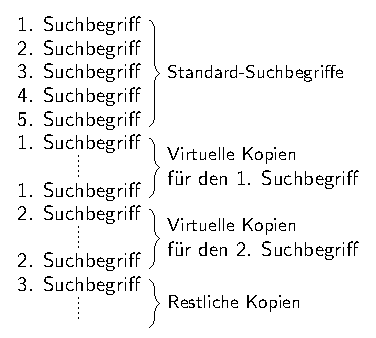
\includegraphics[width=0.4\textwidth]{Bilder/Daemon/VirtualCopies.pdf}
\caption{Die Aufteilung der virtuellen Kopien zu den einzelnen Suchbegriffen. Diese Liste wird anschließend an einen \texttt{Minion} zur Abarbeitung übergeben. \label{figure:daemon_virt_copies}}
\end{figure}

Wie der Abbildung zu entnehmen ist, besitzen junge Suchbegriffe insgesamt $(a - c)$ Anfragen mehr als alte und $(a - b)$ Anfragen mehr als etwas ältere Suchbegriffe.
Zudem haben etwas ältere Suchbegriffe $(b - c)$ Anfragen mehr zur Verfügung als alte Suchbegriffe. Durch diese Priorisierung anhand von virtuellen Kopien wird der Datenbestand für jüngere Begriffe schneller aufgefüllt als bei älteren. 

Momentan ist die Aufteilung für virtuelle Kopien wie folgt:
\begin{itemize}
\item Der Suchbegriff ist weniger als einen Tag alt: 2 weitere virtuelle Kopien
\item Der Suchbegriff ist weniger als eine Woche, aber mindestens einen Tag alt: 1 weitere virtuelle Kopie
\item Der Suchbegriff ist älter als eine Woche: keine weiteren virtuellen Kopien
\end{itemize}

Die Suchstrategie des Daemons zu einem Suchbegriff wird also beeinflusst durch
\begin{itemize}
\item die Intervalllänge für des Suchbegriffes,
\item die durch den Benutzer vorgegebene Priorität zu dem Suchbegriff,
\item das Aktivitätsverhalten des Suchbegriffs, das den Suchbegriff als \textit{short} oder \textit{long term} klassifiziert und
\item das Alter des Suchbegriffs, was zu einer unterschiedlichen Anzahl an virtuellen Kopien und somit zu einer unterschiedlichen Anzahl von Anfragen zum Suchbegriff führt. 
\end{itemize}

\subsection{Parallele Suche} % Jens
\label{ssection:parallele-suche}
\subsubsection{Motivation}
Nachdem der Daemon in der Lage ist mit einer gewissen Intelligenz Tweets zu suchen, könnte man annehmen der Daemon sei fertig.
Für Untersuchungen im kleineren Umfang ist das prinzipiell auch korrekt, uns war die Menge der gefundenen Tweets aber nicht hoch genug.
Wie sich aus den Beschränkungen der Twitter-API, die in Abschnitt \ref{sssection:twitter-api} beschrieben wurden, ergibt, kann der Daemon mit einem Profil maximal 18.000 Tweets in 15 Minuten sammeln.
Das ist vergleichsweise wenig, besonders wenn die Anzahl der Suchbegriffe steigt und auch sehr aktive Suchbegriffe, das heißt Suchbegriffe zu denen es aufgrund gesteigerten Interesses sehr viele Tweets gibt, dabei sind.
Ein Beispiel für einen sehr aktiven Suchbegriff war \textit{walker}.
Mit diesem \textit{search term} konnte man sehr viele Tweets zum Tod von Schauspieler Paul Walker, am 30. November 2013 finden, insgesamt ca. 11 Millionen innerhalb weniger Tage.
Diese Zahlen berichtete zumindest Topsy\footnote{\url{www.topsy.com}}, sie sind aber leider nicht mehr abrufbar, allerdings findet sich im November/Dezember 2013 auch bei Google Trends \cite{GoogleTrendsWalker14} ein entsprechender Ausschlag im Interesse.
Die Anzahl Tweets war zu groß, als dass unser Daemon sie alle hätte finden können.
Das liegt daran, dass der Daemon, wie in Abschnitt Twitter-API \ref{sssection:twitter-api} beschrieben, maximal 18.000 Tweets in 15 Minuten abrufen kann und wir über die Suche maximal 6-9 Tage zurückliegende Tweets finden können.
Da wir noch mehr als diesen einen Suchbegriff bearbeiten, ist es in dem zur Verfügung stehenden Zeitfenster von 6-9 Tagen also nicht möglich alle Tweets zu diesem Thema zu erfassen.
Deswegen wurde als nächstes Ziel entschieden, den Durchsatz zu erhöhen.
Der für uns nächstliegendste Ansatz war der Einsatz mehrerer Profile, immerhin erlaubt jedes weitere Profil den Abruf von bis zu 18.000 weiteren Tweets.
Um mehrere Profile optimal auszunutzen, müssen sie  parallel genutzt werden.
Das erlaubt sowohl die parallele Suche nach verschiedenen Suchbegriffen, als auch nacheinander mit verschiedenen Profilen nach einem Suchbegriff zu suchen.
Da die Suche selbst auch einige Zeit in Anspruch nimmt, kann dies nicht beliebig gesteigert werden, erlaubt aber doch eine gewisse Skalierung.
Gerade auch im Bezug auf eine steigende Zahl von Suchbegriffen erlaubt dies eine höhere Anzahl von gefundenen Tweets.

\subsubsection{Architektur} % Master - Worker - Aufbau - Minions 
Das Parallelisieren erfolgt in einer klassischen Master-Worker-Architektur, bei der ein Master Aufgaben an mehrere Worker verteilt und ihre Ergebnisse sammelt.
Dies erfordert eine Überarbeitung unserer bestehenden Architektur.
Unser Master heißt auch \texttt{Master}, während wir unsere Worker \texttt{Minions} genannt haben.
Außerdem soll der Daemon jetzt dauerhaft laufen und nicht wie vorher nur alle 15 Minuten durch einen \textit{cronjob} gestartet werden.
Dabei ist der \texttt{Master} für die Verwaltung der Profile und die Aufteilung der Suchbegriffe auf die \texttt{Minions} zuständig, während die \texttt{Minions} selbst nur die Tweets von Twitter abrufen und speichern sollen.

\subsubsection{Architektur: Master}% Der Master
Die Suchbegriffe holt sich der \texttt{Master} aus der Datenbank, nachdem er sie in \textit{short} und \textit{long terms} eingeteilt hat (siehe Suchstrategie \ref{ssection:Suchstrategie}), erhält der erste \texttt{Minion} mit einem gültigem Profil, d.\,h. mit einem Profil das noch freie Suchanfragen hat, eine bestimmte Anzahl davon und beginnt mit der Suche.
Wie der \texttt{Master} Suchbegriffe aus der Datenbank abruft und an die \texttt{Minions} verteilt ist in Grafik \ref{img:daemonarchitektur1} dargestellt.
%Wenn der \texttt{Master} gestartet wird und sowohl aktive Suchbegriffe als auch gültige Profile, d.\,h. Profile mit offenen Anfragen, hat, startet er einen \texttt{Minion} und teilt ihm Suchbegriffe zu.
Dabei merkt der \texttt{Master} sich, welche Suchbegriffe er schon verteilt hat, und registriert auch, wenn ein \texttt{Minion} mit seiner Arbeit fertig ist, seine Suchbegriffe also wieder frei werden.
Ursprünglich ging der \texttt{Master} davon aus, dass alle Profile gültig sind, wenn er gestartet wird. Falls dem nicht so war konnte das dazu führen, dass der \texttt{Master} in einer Art Endlos-Schleife lief, dies aber nur temporär.
%TODO eine temporäre Endlos-Schleife ??
In der Schleife hat der \texttt{Master} immer wieder einen \texttt{Minion} erzeugt. Dieser hat sich aber sofort wieder beendet, weil er keine Anfragen mehr frei hatte.
Da der \texttt{Master} die Profile der Reihe nach durchgeht, hängt er so lange in der Schleife bis das Profil wieder gültig wird.
Um diese Problematik zu beheben, wurde die Abfrage der noch freien Anfragen von den \texttt{Minions} in den \texttt{Master} verlagert.
Dadurch weiß der \texttt{Master} immer, ob ein Profil gültig ist.
Wenn der \texttt{Master} keine gültigen Profile oder keine aktiven Suchbegriffe mehr hat, schläft er für einen gewissen, einstellbaren Zeitraum, bevor er erneut prüft, ob es aktive Suchbegriffe und gültige Profile gibt.

\begin{figure}[ht]
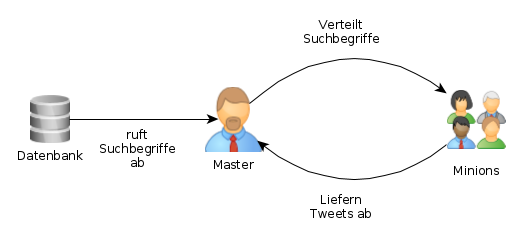
\includegraphics[width=\textwidth]{Bilder/Daemon/DaemonArchitektur1.png}
\caption{Der \texttt{Master} holt Suchbegriffe aus der Datenbank und verteilt sie an die \texttt{Minions}.}
\label{img:daemonarchitektur1}
\end{figure}

\subsubsection{Architektur: Minions} % Die Minions: wie arbeiten sie - speichern selber tweets -> überleitung treasurer
Die Hauptaufgabe der \texttt{Minions} ist das Suchen und Speichern von Tweets.
Große Teile dieser Aufgaben konnten direkt aus dem Code der vorherigen \texttt{single-threaded} Anwendung übernommen werden.
Die Suchbegriffe, die jeder \texttt{Minion} bearbeitet, erhält er dabei direkt vom \texttt{Master}, sodass sich die \texttt{Minions} nicht darum kümmern müssen, welche Begriffe aktiv und noch nicht von anderen \texttt{Minions} belegt sind.
Der \texttt{Master} erhält die Suchbegriffe dabei über den \texttt{Transactor}, der Schnittstelle zur Datenbank, direkt aus der Datenbank.
Sobald ein \texttt{Minion} alle seiner Anfragen aufgebraucht hat, hat er sie über den \texttt{Transactor} in der Datenbank gespeichert.
Es musste sichergestellt werden, dass nicht mehrere \texttt{Minions}, oder ein \texttt{Minion} und der \texttt{Master} gleichzeitig oder in der falschen Reihenfolge auf den gleichen Suchbegriff zugreifen.
Schlimmstenfalls könnte es sonst passieren, dass zwei \texttt{Minions} in der falschen Reihenfolge versuchen, denselben Suchbegriff zu updaten und das Programm dabei abstürzt.
Dies würde zu inkonsistenten Werten bei dem Suchbegriff und damit verlorenen Tweets, d.\,h. Tweets die wir zwar finden könnten, aber nicht erfasst haben, führen.
Auch würden so Anfragen verschwendet, wenn der \texttt{Master} einen neuen \texttt{Minion} zu einem Suchbegriff gestartet hat, der mit genau den gleichen Parametern schon vom vorherigen \texttt{Minion} bearbeitet wurde, diese Werte aber noch nicht in der Datenbank aktualisieren konnte.
Ebenfalls stellte sich schnell heraus, dass die Datenbank-Performance erheblich darunter gelitten hat, wenn zwei \texttt{Minions} gleichzeitig ihre Tweets gespeichert haben.


\subsubsection{Architektur: Treasurer}% Tweets Zentral speichern / Treasurer #1
Um das Problem zu lösen, entschieden wir uns dafür, das Speichern der Tweets und das Aktualisieren der Suchbegriffe an eine zentrale Stelle auszulagern.
Das geschieht, indem die \texttt{Minions} die Tweets, die sie erhalten haben, zusammen mit den entsprechenden und aktualisierten Suchbegriffen beim \texttt{Master} abliefern.
Der \texttt{Master} aktualisiert daraufhin sein lokales \texttt{SearchTerm}-Objekt und speichert die erhaltenen Tweets zwischen.
Dabei stellen alle Tweets inklusive des dazugehörigen Suchbegriffs und seiner Parameter ein \texttt{Package} dar.
Alle \texttt{Packages} werden in einem Beutel gesammelt und nach dem Datum des letztens Abrufs sortiert.
Der Beutel ist dabei, ähnlich wie die \texttt{Treasury} ein virtuelles Konstrukt, in diesem Fall für einen Zwischenspeicher, um \texttt{Packages} zu sammeln.
So stellen wir sicher, dass die \texttt{Packages} in der richtigen Reihenfolge in der Datenbank gespeichert werden.
Falls wir das nicht täten, könnten wir Tweets verlieren.
Wenn der \texttt{Master} von der Datenbank neue Suchbegriffe erhält, vergleicht er sie mit seinen lokalen Objekten.
Solange seine lokalen Objekte neuere Werte haben als die Werte, die die Datenbank liefert, werden die lokalen verwendet.
Ausschlaggebendes Kriterium dafür, wie aktuell ein Suchbegriff ist, ist der Zeitpunkt der letzten Suche.

\begin{figure}[ht]
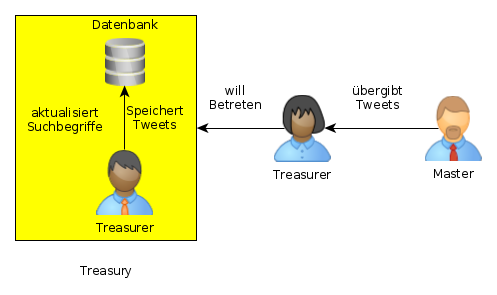
\includegraphics[width=\textwidth]{Bilder/Daemon/DaemonArchitektur2.png}
\caption{Der \texttt{Master} übergibt die gesammelten Tweets einem \texttt{Treasurer}. Ein weiterer \texttt{Treasurer} speichert Tweets in die Datenbank.}
\label{img:daemonarchitektur2}
\end{figure}

%Tweets Zentral speichern / Treasurer #2
Der \texttt{Master} soll nicht selbst die Tweets speichern, da er zum einen weiterhin neue Tweets der \texttt{Minions} entgegennehmen, zum anderen auch die Suchbegriffe verteilen muss.
Um dies zu umgehen, wurde ein neuer \texttt{Worker} erschaffen, dessen einzige Aufgabe das Speichern von Tweets ist.
Wir haben ihn \texttt{Treasurer} genannt, analog dazu gibt es auch eine \texttt{Treasury}, eine Schatzkammer.
Die \texttt{Treasury} ist dabei ein virtuelles Konstrukt, das den Zugang zur Datenbank bildlich darstellt.
Der \texttt{Master} wartet entweder, bis er mindestens eine gewisse Anzahl von Tweets in seinem Beutel gesammelt hat, oder bis eine einstellbare Zeit nach dem Ende des letzten \texttt{Treasurer} vergangen ist, bis er einen neuen \texttt{Treasurer} erzeugt.
Es kann dabei durchaus mehrere \texttt{Treasurer} gleichzeitig geben, wenn sehr viele Tweets in kurzer Zeit gefunden werden, oder die alten \texttt{Treasurer} noch nicht mit ihrer Arbeit fertig sind, wenn ein neuer erzeugt wird.
Der \texttt{Treasurer} erhält eine Kopie des Beutels vom \texttt{Master} und dieser leert anschließend seinen Beutel.
Nun versucht der \texttt{Treasurer} die \texttt{Treasury} zu betreten.
Wie der Master die gesammelten Tweets an einen \texttt{Treasurer} übergibt, während ein weiterer \texttt{Treasurer} Tweets in der Datenbank speichert, ist in Grafik \ref{img:daemonarchitektur2} dargestellt.
Die \texttt{Treasury} ist dabei als Mutex realisiert und stellt somit auch eine Warteschlange für die \texttt{Treasurer} da.
Versucht ein \texttt{Treasurer} die \texttt{Treasury} zu betreten, heißt das, dass er versucht das Mutex zu erlangen.
Gelingt ihm das Betreten der \texttt{Treasury}, also das Erlangen des Mutex, speichert er alle Tweets aus seinem Beutel in der Datenbank, genau wie es der alte Daemon vorher getan hat.
Außerdem aktualisiert er die \texttt{SearchTerms} in der Datenbank, allerdings erst, nachdem er die zu dem Suchbegriff gehörenden Tweets gespeichert hat.
Falls der Daemon abstürzt oder beendet wird, bevor der Suchbegriff aktualisiert wurde, sind die Tweets trotzdem vorhanden und werden schlimmstenfalls erneut gefunden.
Würde aber erst der \texttt{SearchTerm} aktualisiert und danach erst die Tweets gespeichert, wären alle Tweets verloren, die nicht mehr gespeichert wurden.
Das liegt daran, dass der Daemon aufgrund seiner Suchstrategie davon ausgeht, dass die Tweets schon gespeichert sind.
Anschließend informiert er gegebenenfalls andere wartende \texttt{Treasurer} über das Ende seiner Arbeit und beendet sich.
Sollte die \texttt{Treasury} belegt sein, schläft ein \texttt{Treasurer} und wartet auf eine Benachrichtigung durch den die \texttt{Treasury} belegenden \texttt{Treasurer}.
In der letzten Scrum-Iteration des Projektseminars wurde die Art, wie der \texttt{Treasurer} die Tweets in der Datenbank speichert, angepasst.
Waren es zuerst jeweils einzelne Tweets, die gespeichert wurden, wurde das System auf \textit{batch inserts} umgestellt.
Dabei fügt der \texttt{Treasurer} erst eine bestimmte Anzahl von Tweets zu einem \textit{batch} zusammen und speichert dann alle Tweets einer \textit{batch} auf einmal.
Dies brachte teilweise erhebliche Geschwindigkeitsvorteile, auch abhängig von der Größe der \textit{batch}.

\subsubsection{Multi-Threading}
Die parallele Suche an sich wurde mit einem klassischen Master-Worker Modell mit Multi-Threading umgesetzt.
Der \texttt{Master} hat dabei hauptsächlich die verwaltende Tätigkeit, wie oben beschrieben.
Generell ist sowohl der \texttt{Master} als auch jeder \texttt{Minion} und \texttt{Treasurer} ein eigener Thread.
Ein Abstürzen eines einzelnen Threads sollte, solange es sich nicht um den \texttt{Master} handelt, nicht das ganze Programm abstürzen lassen.
Es gab aber an einigen Stellen Schwierigkeiten mit dem Multi-Threading Ansatz.
So müssen die einzelnen Worker mit dem \texttt{Master} interagieren und z.\,B. melden, wenn sie mit ihrer Arbeit fertig sind.
Auch gibt es mehrere Stellen, an denen mehrere Threads um die gleiche Ressource kämpfen, wo es Probleme mit Deadlocks gab.
Ein klassisches Problem war dabei, dass in der \texttt{Treasury} der Mutex nicht überall in der gleichen Reihenfolge erlangt wurde, dies konnte zu Deadlocks führen.
Die Lösung war die Reihenfolge, in der die Mutexe erlangt werden, überall zu vereinheitlichen.
Ein weiteres Problem konnte auftreten, wenn der \texttt{Master} keine freien Suchbegriffe hatte.
Dabei hat er eine \texttt{if}-Abfrage abgebrochen, in dessen Rahmen ein Mutex erlangt wurde, ohne es frei zu geben.
Da die \texttt{Minions} aber denselben Mutex benötigten, um ihre Tweets und Suchbegriffe abzugeben, kam es zu einem Deadlock. Das Finden dieses Fehlers war sehr aufwändig.
Die Lösung, dass der \texttt{Master}, bevor er die Schleife abbricht, noch den Mutex freigibt, ist dagegen recht trivial.
Das Multi-Threading erforderte auch die Einführung der schon oben erwähnten \texttt{Packages}.
Alle Tweets, die ein \texttt{Minion} findet, sind mit dem Suchbegriff, zu dem sie gefunden wurden, sowie den zugehörigen Metadaten zum Zeitpunkt der Suche verknüpft.
Wenn nun nacheinander mehrere \texttt{Minions} denselben Suchbegriff bearbeiten, gäbe es mehrere Tweets, die alle zum selben Suchbegriff gehören, aber mit unterschiedlichen Metadaten assoziiert sind.
Es war also nicht möglich alle Tweets zu einem Suchbegriff im Beutel des \texttt{Master} zu sammeln.
Stattdessen wurden \texttt{Packages} eingeführt.
Jedes \texttt{Package} stellt dabei eine Sammlung der Tweets mit dem assoziierten Suchbegriff eines Suchdurchlaufs dar.
Die einzelnen \texttt{Packages} werden dann nach dem Zeitpunkt der Suche chronologisch sortiert und auch in derselben Reihenfolge abgespeichert.
So wird verhindert, dass im Falle eines Absturzes des Programms Tweets verloren gehen, wenn sie weder gespeichert sind, noch erneut gesucht werden.

 % torsten
\subsection{Zeitnahe Ergebnisse}
\label{ssection:ZeitnaheErgebnisse}
Bislang musste der Benutzer im schlimmsten Fall bis zu 15 Minuten auf Ergebnisse warten, wenn er einen neuen Suchbegriff eingegeben hat.
Denn hatten alle zur Suche verwendeten Profile kurz bevor der Benutzer die Suche zu einem neuen Suchbegriff startete ihr \textit{rate limit} ausgeschöpft, so musste er warten, bis wieder ein Profil frei wurde.
Dies konnte aber wie bereits erwähnt dann bis zu 15 Minuten dauern.
Das war jedoch nicht besonders benutzerfreundlich und wurde daher als Problem angesehen, das es zu beheben galt.

\subsubsection{Motivation}

Es wäre daher besser, wenn der Benutzer einen neuen Suchbegriff eingibt und anschließend nach möglichst kurzer Zeit, maximal nach 20 bis 30 Sekunden, die ersten Ergebnisse seiner Suchanfrage angezeigt bekommt.
Die Anzahl der Ergebnisse muss noch nicht sehr hoch sein; vielmehr genügt es dem Benutzer, wenn er zumindest einen kleinen Datensatz als Grundlage zum Analysieren besitzt.
So kann er sich bereits sehr zeitnah einen ersten Überblick über den Suchbegriff verschaffen.
Zu einem späteren Zeitpunkt haben sich dann wesentlich mehr Daten zum Suchbegriff gefunden, mit denen der Benutzer dann intensiver arbeiten kann.

\subsubsection{Konzept}

Es stellt sich nun die Frage, wie erreicht werden kann, dass bereits sehr zeitnah zur Suchanfrage die ersten Daten präsentiert werden können.
Um das oben geschilderte Problem der aufgebrauchten Twitter-Profile zu umgehen, führen wir ein weiteres Profil ein, das nur genutzt wird, wenn ein neuer Suchbegriff in der Datenbank gefunden wird.
So ist sichergestellt, dass es immer ein Profil gibt, das nach Tweets zum neuen Suchbegriff suchen kann.
Des Weiteren darf dieses gesonderte Profil jedoch nicht sofort für einen neuen Suchbegriff das \textit{rate limit} vollständig aufbrauchen, weswegen die Anzahl der Anfragen an Twitter durch den Daemon begrenzt wird.
Wäre die Anzahl der Anfragen nicht begrenzt, so stünden für einen weiteren, neuen Suchbegriff keine Anfragen mehr zur Verfügung und der Benutzer müsste wieder 15 Minuten warten.
Die maximal zulässige Anzahl an Anfragen für das gesonderte Profil lässt sich beliebig einstellen; ein Grenzwert von 10 hat sich jedoch als akzeptabel herausgestellt.
In diesem Fall verbraucht das Profil also lediglich 10 der 180 Anfragen, weswegen noch 170 Anfragen zur Verfügung stehen.
Es kann also innerhalb von 15 Minuten nach höchstens 18 neuen Suchbegriffen gesucht werden.
Da es jedoch unwahrscheinlich ist, dass in diesem kurzen Zeitraum tatsächlich so viele neue Suchbegriffe hinzukommen, ist diese Limitierung als nicht-kritisch anzusehen.

Mit 10 Anfragen lassen sich bis zu 1000 Tweets zu einem neuen Suchbegriff finden, was eine akzeptable erste Datenbasis schafft.
Möchte man mehr Tweets finden, so muss der Grenzwert der Anfragen an Twitter hochgestellt werden.
In diesem Fall können jedoch nicht 18 neue Suchbegriffe innerhalb von 15 Minuten gefunden werden, sondern es sind weniger.
Ein Verringern des Grenzwertes liefert zwar weniger Tweets, doch kann der Benutzer dann mehr als 18 neue Suchbegriffe innerhalb der 15 Minuten eingeben.

Es sollte jedoch bedacht werden, dass ein geringer Grenzwert mit wenigen Anfragen auch weniger Zeit für die Suche nach Tweets benötigt als ein höherer Grenzwert mit mehr Anfragen.

\begin{figure}[h!]
\centering

\begin{subfigure}[t]{0.5\textwidth}
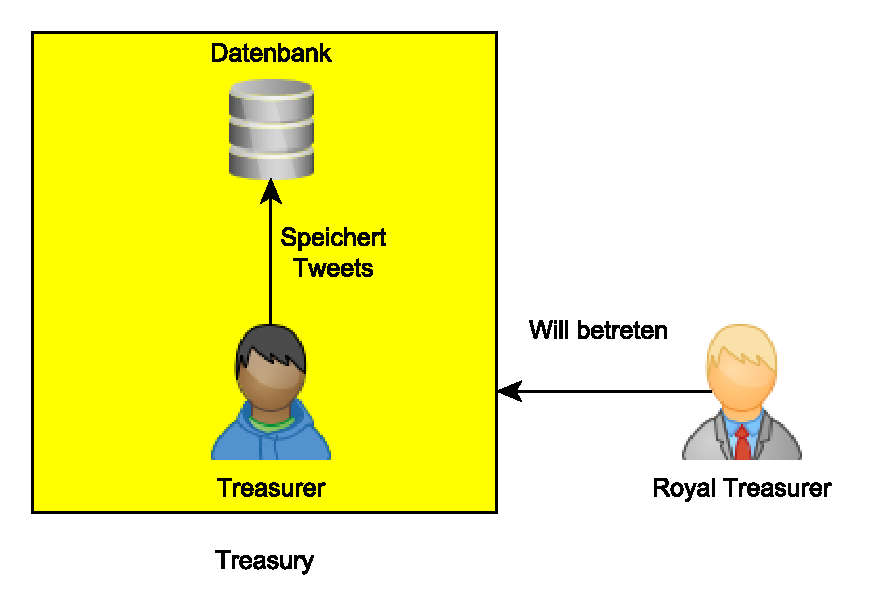
\includegraphics[width=\textwidth]{Bilder/Daemon/RoyalTreasurer1.pdf}
\caption{Ein \texttt{Royal Treasurer} will die \texttt{Treasury} betreten.}
\label{fig:royal_treasurer1}
\end{subfigure}
~
\begin{subfigure}[t]{0.3\textwidth}
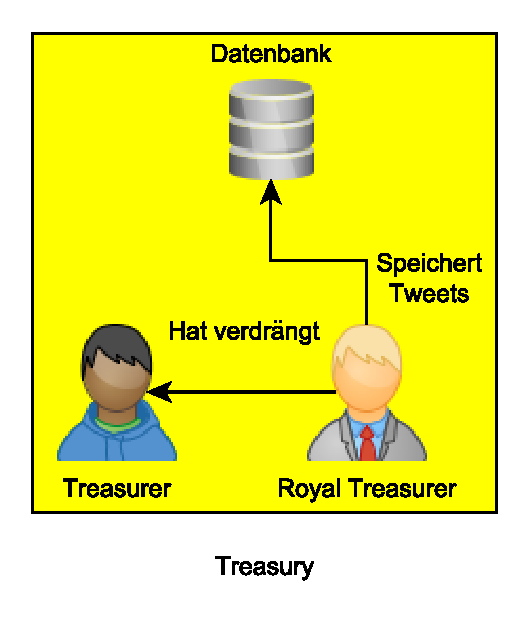
\includegraphics[width=\textwidth]{Bilder/Daemon/RoyalTreasurer2.pdf}
\caption{Der \texttt{Royal Treasurer} verdrängt den \texttt{Treasurer}.}
\label{fig:royal_treasurer2}
\end{subfigure}

\begin{subfigure}[t]{0.3\textwidth}
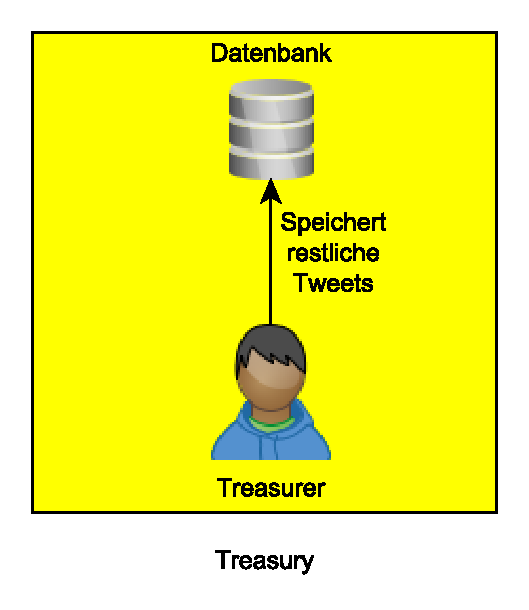
\includegraphics[width=\textwidth]{Bilder/Daemon/RoyalTreasurer3.pdf}
\caption{Der verdrängte \texttt{Treasurer} setzt seine Arbeit fort.}
\label{fig:royal_treasurer3}
\end{subfigure}
\end{figure}

Das besondere Profil alleine hilft allerdings noch nicht dabei, dass der Benutzer auch zeitnah die gefundenen Tweets angezeigt bekommt.
Bislang ist lediglich sichergestellt, dass der Daemon auf jeden Fall nach einem neuen Suchbegriff suchen kann.
Bis die Ergebnisse allerdings dem Benutzer auch tatsächlich präsentiert werden können, kann jedoch ebenfalls einige Zeit vergehen, da die Tweets noch nicht in der Datenbank gespeichert wurden.
Stattdessen werden sie zunächst im Beutel des \texttt{Masters} hinterlegt, welcher jedoch nicht zwingend umgehend durch einen \texttt{Treasurer} geleert werden muss.
Da der \texttt{Treasurer} eine vorgegebene Zeit wartet, bis er den Beutel des \texttt{Masters} leert, oder er den Beutel leert, falls die festgelegte Zahl der Tweets im Beutel überschritten wird, kann es teilweise sehr lange dauern, bis die neuen Tweets in die Datenbank geschrieben wurden.
Der Benutzer musste also weiterhin lange auf die ersten Ergebnisse warten.

Um das Problem zu umgehen, wird ein weiterer Beutel eingeführt, der ausschließlich für die zeitnahen Tweets genutzt wird.
Wurde dieser Beutel befüllt, wird er -- unabhängig davon, wann er zuletzt befüllt worden ist oder wie voll er ist -- sofort von einem \texttt{Treasurer} geleert, damit die Tweets auch sofort in die Datenbank geschrieben werden können.
Somit wurde die Wartezeit bis zur Leerung des Beutels eliminiert.
Dies hilft allerdings immer noch nicht zwingend.
Denn es kann durchaus vorkommen, dass bereits ein anderer \texttt{Treasurer} in der \texttt{Treasury} aktiv ist und unser wichtigerer \texttt{Treasurer} warten muss, was bedeutet, dass auch der Benutzer warten muss.
Aus diesem Grund erhält der \texttt{Treasurer}, der den besonderen Beutel leert, eine höhere Priorität gegenüber anderen \texttt{Treasurern}.
Um die höhe Priorität anzudeuten, wird dieser \texttt{Treasurer} deswegen \texttt{Royal Treasurer} genannt.
Betritt dieser nun die \texttt{Treasury}, verdrängt er einen möglicherweise aktiven \texttt{Treasurer} und kann somit seine Tweets sofort abspeichern.
Ist er mit dem Abspeichern fertig, so weckt er den verdrängten Treasurer wieder auf, sodass dieser seine Arbeit an dem Punkt fortsetzen kann, an dem er unterbrochen wurde.
Die Abbildungen \ref{fig:royal_treasurer1}, \ref{fig:royal_treasurer2} und \ref{fig:royal_treasurer3} illustrieren diese Situation.

Es kann vorkommen, dass es zeitweise mehrere \texttt{Royal Treasurer} gibt, nämlich genau dann, wenn mehrere Suchbegriffe zeitnah neu eingegeben werden.
Tritt diese Situation ein, so werden die \texttt{Royal Treasurer} sequentiell in der Reihenfolge, in der sie die \texttt{Treasury} betreten, aktiv.
Ein möglicherweise zuvor verdrängter \texttt{Treasurer} muss dann die gesamte Zeit lang warten, bis alle Royal \texttt{Treasurer} fertig sind.

\subsubsection{Implementierung}

Das besondere Profil wird von einem besonderen \texttt{Minion} genutzt, der darauf achtet, dass der zuvor gesetzte Grenzwert von beispielsweise zehn Anfragen auch beachtet wird.
Die anderen \texttt{Minions} suchen nämlich so lange zu Suchbegriffen, bis ihr \textit{rate limit} aufgebraucht ist.
Der besondere \texttt{Minion} wird von uns \texttt{Limited Minion} genannt, da er nur eine begrenzte (engl.: \textit{limited}) Anzahl an Anfragen an Twitter stellt.
Der \texttt{Limited Minion} teilt, nachdem er seine Suche abgeschlossen hat, dem \texttt{Master} über eine gesonderte Nachricht mit, dass er fertig ist.
Aufgrund dieser gesonderten Nachricht weiß der \texttt{Master} anschließend, dass es sich um den \texttt{Limited Minion} handelt, weswegen der \texttt{Master} entsprechend ein sofortiges Leeren des besonderen Beutels durch den \texttt{Royal Treasurer} einleitet.

Dieser \texttt{Royal Treasurer} $R$ betritt nun die \texttt{Treasury} und versucht das Mutex der \texttt{Treasury} zu erhalten.
Es kann jedoch sein, dass bereits irgendein (\texttt{Royal}) \texttt{Treasurer} $A$ aktiv in der \texttt{Treasury} arbeitet und $R$ das Mutex nicht erhalten kann, weswegen er kurzzeitig warten muss.
Ist $A$ ein anderer \texttt{Royal Treasurer}, so muss $R$ weiterhin warten, da er andere \texttt{Royal Treasurer} nicht verdrängen darf.
Ist $A$ hingegen ein normaler \texttt{Treasurer}, so darf $R$ $A$ verdrängen.
Dies tut $R$ jedoch nur indirekt.
Während nämlich $A$ seine Tweets in kleineren Paketen abspeichert, schaut er immer wieder nach, ob in der \texttt{Treasury} ein \texttt{Royal Treasurer} wartet.
Falls dies der Fall ist, gibt $A$ das Mutex frei und legt sich schlafen, bis er wieder durch einen fertig gewordenen \texttt{Royal Treasurer} aufgeweckt wird.
Hat $A$ nun das Mutex freigegeben, blockiert $R$ es sofort und beginnt anschließend, seine Tweets abzuspeichern.
Ist $R$ fertig, informiert er den schlafenden $A$ darüber und weckt diesen auf.
Anschließend gibt $R$ das Mutex wieder frei, welches $A$ dann sofort wieder sperrt.
Sicherheitshalber prüft $A$ anschließend sofort noch einmal, ob nicht schon wieder ein anderer \texttt{Royal Treasurer} wartet.
Ist dies der Fall, legt sich $A$ direkt wieder schlafen.

(\texttt{Royal}) \texttt{Treasurer} können das \texttt{Treasury}-Mutex nicht direkt verwenden. Vielmehr wird das Betreten oder Verlassen der \texttt{Treasury} und das damit einhergehende Sperren und Entsperren des Mutexes durch die \texttt{Treasury} verwaltet.
So ist die Konsistenz innerhalb des Arbeitsflusses unter den einzelnen (\texttt{Royal}) \texttt{Treasurern} gewährleistet.

% torsten
\subsection{Diskussion}
\label{ssection:ausblick}
Obwohl der Daemon gemäß der Kundenwünsche als fertig bezeichnet werden kann, hätte er dennoch um einige Aspekte erweitert werden können, sofern mehr Zeit zur Verfügung gestanden hätte.

\subsubsection{Verbesserte parallele Suche}

Bislang ist es nicht möglich, dass mehrere \texttt{Minions} zu einem Suchbegriff parallel suchen.
Dies wäre jedoch wünschenswert, um beispielsweise Suchbegriffe, die temporär eine extreme Aktivität verzeichnen (beispielsweise aufgrund eines unvorhersehbaren Vorkommnis in Zusammenhang mit dem Suchbegriff) besser abzuarbeiten.
Besonders problematisch wird es, wenn zu diesen Suchbegriffen innerhalb von wenigen Stunden eine Anzahl von mehreren Millionen Tweets anfällt.
Denn dann kann der Daemon in seiner bisherigen Form die große Datenlast nicht vollständig abarbeiten, da nach 6-9 Tagen die Tweets von Twitter nicht mehr bereitgestellt werden, der Daemon jedoch noch nicht alle Tweets der gesteigerten Aktivität gesammelt hat.
So gehen unerwünschterweise Daten verloren.

Könnten jedoch stattdessen mehrere \texttt{Minions} parallel zu einem solchen Suchbegriff suchen, steigt die Bearbeitungsgeschwindigkeit der Tweets linear in der Anzahl der parallel arbeitenden \texttt{Minions}.
Eine Umsetzung dieser Idee stellt sich jedoch als schwierig dar, da Twitter es nicht ermöglicht, eine Suche auf Zeitintervalle geringer als einen Tag einzuschränken.

Dies ist jedoch nötig, da die riesige Datenmenge nicht nur über Tage gestreut ist, sondern eben bereits über Stunden, teilweise sogar über Minuten.
Daher ist eine Beschränkung der Suche auf Stunden- oder Minutenintervalle wünschenswert.
Da dies jedoch nicht möglich ist, muss als alternativer Weg die Suche über die IDs einzelner Tweets stattfinden.
Hierbei wäre es die grundlegende Idee, den verstrichenen Zeitraum $s$ zwischen dem ältesten ($t_o$) und dem neusten Tweet ($t_n$) einer einzelnen Suchanfrage zu betrachten.
Anschließend berechnet man die Differenz $d$ der beiden IDs der betrachteten Tweets $t_o$ und $t_n$ und geht nun davon aus, dass über einen Zeitraum $s$ insgesamt $d$ viele neue Tweets veröffentlicht werden.
Nun wird dieser Zeitraum $s$ $n$-mal in die Vergangenheit zurück gegangen bis zu dem Zeitpunkt, ab dem man einen weiteren \texttt{Minion} suchen lassen möchte, wobei das $n$ selbst gewählt wird.
Um nun tatsächlich ab diesem Zeitpunkt zu suchen, wird die zuvor erhaltene Differenz $d$ ebenfalls $n$-mal von der ID des Tweets $t_n$ subtrahiert. Ab dieser ID kann dann ein neuer \texttt{Minion} suchen.
Dieses Verfahren garantiert jedoch \emph{absolut nicht}, dass die berechnete Tweet-ID auch tatsächlich zu dem gewünschten Zeitpunkt gehört.
Vielmehr ist die berechnete Tweet-ID eine \emph{sehr grobe} Schätzung des gewünschten Zeitpunkts.

Das Verfahren ist also in der Theorie bereits nicht besonders vielversprechend.
Mit dem dazu verbundenen hohen Implementierungsaufwand sowie einer Umstellung des Datenbankschemas wurde dieser Ansatz also verworfen, da er nicht vernünftig in kurzer Zeit realisierbar gewesen wäre.

\subsubsection{Profile}

Zum jetzigen Zeitpunkt ist es nicht möglich, weitere Twitter-Profile zur Laufzeit hinzuzufügen oder zu entfernen.
Um dies zu erreichen, muss der Daemon explizit beendet und neu gestartet werden.
Das ist jedoch umständlich und kostet unnötig Zeit.
Das erwartete Verhalten ist vielmehr, dass der Daemon automatisch erkennt, wenn ein neues Twitter-Profil im entsprechenden Verzeichnis vorliegt oder plötzlich fehlt.
Entsprechend sollte der Daemon in diesen Fällen dann darauf reagieren.

Aus Zeitgründen und der Tatsache, dass ein solches Verhalten lediglich eine Komforteigenschaft ist, wurde jedoch auf eine Implementierung verzichtet.

\subsubsection{Logging}

Der Daemon nutzt für das Festhalten von Fehlern, Warnungen oder anderen Informationen ein minimalistisches Logging-System, welches selbst implementiert wurde.
Auf die Nutzung einer Logging-Bibliothek wurde verzichtet.
Der Entschluss für den Verzicht wurde wieder aufgrund der Zeitbegrenzung getroffen.
Das selbst implementierte Logging-System unterstützt neben der totalen Basis des Loggings einzelnen Meldungen nahezu keinerlei weitere Funktionalität.
Lediglich die Verwendung der Log-Datei ähnlich zu einem Ringpuffer wird noch unterstützt.
Das bedeutet, dass die entsprechende Log-Datei nicht mehr Zeilen als spezifiziert haben soll.
Tritt dieser Fall ein, so werden die ältesten Log-Einträge gelöscht, da diese vermutlich keine bis wenig Relevanz mehr haben.

Der Entschluss gegen die Verwendung einer robusteren und im Funktionsumfang größeren Logging-Bibliothek fiel, da sowohl die Verwendung der von Java selbst bereitgestellten Klassen als auch der Bibliothek Log4J komplex und schwierig ist und viel Einarbeitungszeit benötigt hätte \cite{log4J}.
Es war daher schneller, ein eigenes minimalistisches Logging-System zu entwickeln, das unsere Anforderungen bezüglich des Loggings erfüllt.
Eine nachträgliche Integration einer externen Logging-Bibliothek in den Daemon und das Entfernen des aktuellen Loggings sollten allerdings nicht zu aufwändig sein, sofern der Entwickler gut mit der externen Bibliothek vertraut ist und genau weiß, wie sie zu verwenden ist.

\subsubsection{Sentiment-Auslagerung}

Das Sentiment (siehe dazu Abschnitt \ref{sec:Sentiment}) von Tweets wird momentan im Daemon berechnet.
Hierbei ergeben sich jedoch ein paar Probleme.
Zum einen kann es zu inkonsistenten Sentiment-Einträgen in der Datenbank kommen, falls das Sentiment gerade aktualisiert wird und der Daemon unerwartet beendet wird oder abstürzt.
Dieses unerwartete Verhalten möchte man vermeiden.
Des Weiteren benötigt das Sentiment zeitweise sehr viele Ressourcen was Speicherverbrauch und CPU-Belastung betrifft.
Zudem wird die Datenbank -- welche permanent mit neuen Tweets befüllt wird -- durch das Sentiment-Update belastet, weswegen das Abspeichern neuer Tweets massiv verlangsamt und so die Effizienz des Daemons negativ beeinflusst wird.

Aus diesen Gründen ist es eine Überlegung wert, das Sentiment in ein eigenes Programm auszulagern und völlig vom Daemon zu entkoppeln.
Dies bringt mehrere Vorteile mit sich.
So beeinflusst das Beenden des Daemons das Sentiment nicht, weswegen es aus diesem Grund auch nicht mehr zu inkonsistenten Sentiment-Einträgen in der Datenbank kommen kann.
Ein Absturz des Sentiment-Prozesses, der dann zu inkonsistenten Werten sorgt, ist allerdings weiterhin möglich.
Ein weiterer Vorteil der Auslagerung ist die erhöhte Performance des Daemons zu Zeiten der Sentiment-Aktivität, da beide Aspekte -- die Suche nach Tweets und das Updaten des Sentiments -- nicht mehr um die gemeinsamen Ressourcen konkurrieren.
Stattdessen hat jeder Prozess seine eigenen Ressourcen zur Verfügung, die optimal ausgenutzt werden können.
Ebenfalls kann nun extern die Priorität der einzelnen Programme, Daemon und Sentiment, geregelt werden.
Hierbei ist beispielsweise eine niedrige Priorität für den Sentiment-Prozess sinnvoll, da Änderungen innerhalb der Datenbank nicht sofort verfügbar sein müssen, sondern über einen längeren Zeitraum eingepflegt werden sollen.
Zudem lässt sich auch innerhalb der Datenbank die Priorität regeln.
So ist es wünschenswert, dass der REST-Service die höchste Priorität beim Arbeiten mit der Datenbank hat, da der Benutzer möglichst schnell Antworten erhalten möchte.
Der Daemon sollte niedriger priorisiert sein, um den REST-Service nicht zu behindern.
Allerdings sollte die Priorität vom Daemon immer noch höher als die vom Sentiment-Prozess sein, um die zuvor genannten Effizienz nicht negativ zu beeinflussen.

Ein Nachteil der Auslagerung ist, dass das Sentiment für neue Tweets nicht mehr sofort bestimmt wird.
Da das Sentiment bislang im Daemon angesiedelt ist, kann, während ein neuer Tweet in die Datenbank eingepflegt wird, auch sofort das Sentiment für diesen Tweet bestimmt und mit abgespeichert werden.
Eine Auslagerung in ein eigenes Programm würde nun bedeuten, dass das Sentiment für neue Tweets zunächst unbestimmt ist und erst zu einem späteren Zeitpunkt berechnet werden kann.

Die Vorteile eine Auslagerung des Sentiments aus dem Daemon überwiegen jedoch gegenüber den Nachteilen, weswegen das Trennen beider Komponenten sinnvoll wäre.

\subsubsection{Speicherverbrauch}

Während der letzten Iteration des Projektseminars traten leider massive Speicherprobleme innerhalb des Daemons auf, die das Programm häufig abstürzen schließen und so einen Produktiveinsatz unmöglich machten.
Aus diesem Grund wurden daraufhin einige Speicheroptimierungen durchgeführt, die das Problem behoben haben.
Dennoch ist die Verwendung des Speichers innerhalb des Daemons immer noch nicht optimal und ließe sich sicherlich an einigen Stellen verbessern.
Aus Zeitgründen -- primär aber, weil das Problem erst viel zu spät bekannt wurde -- konnte neben den rudimentären Optimierungen hierauf jedoch nicht weiter eingegangen werden.

\subsubsection{Daemon-API}

Es gibt zur Zeit keine komfortable Möglichkeit, Informationen über den Daemon abzufragen.
Um zu wissen, was der Daemon gerade macht, muss in die entsprechende Log-Datei geschaut werden und jeder einzelne Log-Eintrag analysiert werden.
Das ist, insbesondere für einen Menschen, sehr mühselig und fehleranfällig.
Ebenfalls fehlt in der Log-Datei ein großer Anteil an Informationen, die für eine Log-Datei unnötig erscheinen, dennoch interessant zu wissen wären.
Es wäre daher ratsam gewesen, eine Daemon-API zu entwickeln, sodass beispielsweise das Frontend mit dem Daemon kommunizieren kann.
Dieses könnte dann anzeigen, nach welchen Suchbegriffen in diesem Moment mit welchem Twitter-Profil gesucht wird, welche Profile gerade ihr \textit{rate limit} ausgeschöpft haben, ob der \texttt{Treasurer} aktiv ist, wie viele \texttt{Treasurer} warten etc.
Mit solch einer API könnte über den Daemon alles in Erfahrung gebracht werden.

Ebenfalls könnte hierdurch die Architektur bezüglich des \textit{Royal Treasurers} gegebenenfalls wegfallen.
Denn der Daemon könnte dem REST-Service die zeitnah gefundenen Tweets direkt mitteilen und müsste nicht den "`Umweg"' über die Datenbank gehen.
Dies könnte auch sehr viel schneller sein, da keine Datenbankzugriffe nötig sind.
Die Tweets selbst würden dann im normalen Beutel des \texttt{Masters} temporär gespeichert werden und zu einem späteren Zeitpunkt in der Datenbank eingetragen werden.

Da die Daten unter anderem auch lokal gecached werden (siehe hierzu den Abschnitt Service-Klassen in \ref{sec:restUmsetzungen} und den Abschnitt \ref{sec:performance_opt} zu Perfomance-Optimierungen des Servers), würde eine erneute Anfrage zu diesem Suchbegriff auch keine erneute Suche bei Twitter starten.
Problematisch wird es lediglich, wenn der Benutzer seinen lokalen Cache löscht und die Tweets noch nicht in die Datenbank geschrieben wurden.
Unter der Annahme, dass es keinen \texttt{Royal Treasurer} mehr gibt, wird dann eine neue Suche bei Twitter gestartet, die wieder einige Anfragen des besonderen Twitter-Profils verbraucht und genau dieselben Tweets liefert, die bereits im Beutel des \texttt{Masters} liegen.
Das ist zwar unschön, allerdings nicht besonders tragisch und könnte akzeptiert werden.

Da eine Anzeige der Informationen über den Zustand des Daemon im Frontend und gegebenenfalls weitere Features aufgrund der Daemon-API jedoch nicht vom Kunden gewünscht wurden und die verfügbare Zeit stark eingeschränkt war, kam es nicht zur Entwicklung einer Daemon-API.

\section{Datenbank}
%\subsection{Einleitung}
Wie im Kapitel Daemon \ref{sec:daemon} schon angedeutet, ist der Grund für das Verwenden einer Datenbank einerseits den Beschränkungen der Twitter-API geschuldet, andererseits erlaubt uns die Verwendung einer eigenen Datenbank, Twitter-Daten zu erweitern (z.\,B. durch Sentimentwerte).
%Eine relationale Datenbank erlaubt es uns, alle für uns relevanten Daten zu speichern und erst später beliebige Anfragen auf diesen Daten auszuführen.
%Da sich erst im Laufe des Projektseminars herausstellte, welche Werte eines Datensatzes für uns interessant sind, kommt uns dieser Arbeitsansatz sehr entgegen. 
Wie in Kapitel \ref{sec:Tech} erwähnt, wird in unserem Projekt die Datenbank MySQL verwendet.
%TODO Ref

%\subsection{MySQL}
%Die Wahl ist recht schnell auf eine relationale Datenbank, genauer gesagt MySQL, gefallen.
%Das liegt hauptsächlich daran, dass ein Großteil der Projektseminar-Teilnehmer am meisten Erfahrungen mit %SQL und MySQL hatten.
%Wir haben zwar schon von der NoSQL-Datenbank gehört, da diese sich aber deutlich von relationalen Datenbanken unterscheidet, haben wir davon abgesehen, eine solche einzusetzen.
%Der mögliche Einarbeitungsaufwand in ein vollkommen neues System (wie zum Beispiel eine No-SQL-Datenbank), von dem wir nicht sicher waren, dass es unsere Anforderungen erfüllte, erschien uns zu riskant.
%Zudem wissen wir von MySQL, dass es in größeren Umgebungen erfolgreich eingesetzt wird.
%Außerdem erlaubt uns MySQL-Workbench, passende SQL-Statements zum Anlegen einer Datenbank automatisch aus einem relationen Datenbankschema zu generieren. 
%Allerdings konnten wir auch gerade am Beginn des Projektseminars nicht benennen, welche Metriken bei einer Datenbank für uns vorteilhaft wären.
% Anbindung an Java kein Problem
% verweis auf technik

\subsection{Schema} %ERM=Erwin
Unser Anspruch ist, möglichst jede Information, die Twitter uns liefert, auch selbst zu speichern, da gerade zu Beginn des Projektseminars noch nicht abzusehen war, welche Informationen letztendlich genutzt werden.
Deshalb orientiert sich unser Schema sehr stark an der offiziellen Dokumentation von Twitter für Tweets \cite{TwitterTweets} und User \cite{TwitterUsers}. 
Dabei haben wir mit wenigen Ausnahmen fast alle Werte übernommen, die Twitter zur Verfügung stellt.
% zum Beispiel der \textit{source}, welche den Klienten beim Verfassen des Tweets angibt.

\begin{figure}[th]
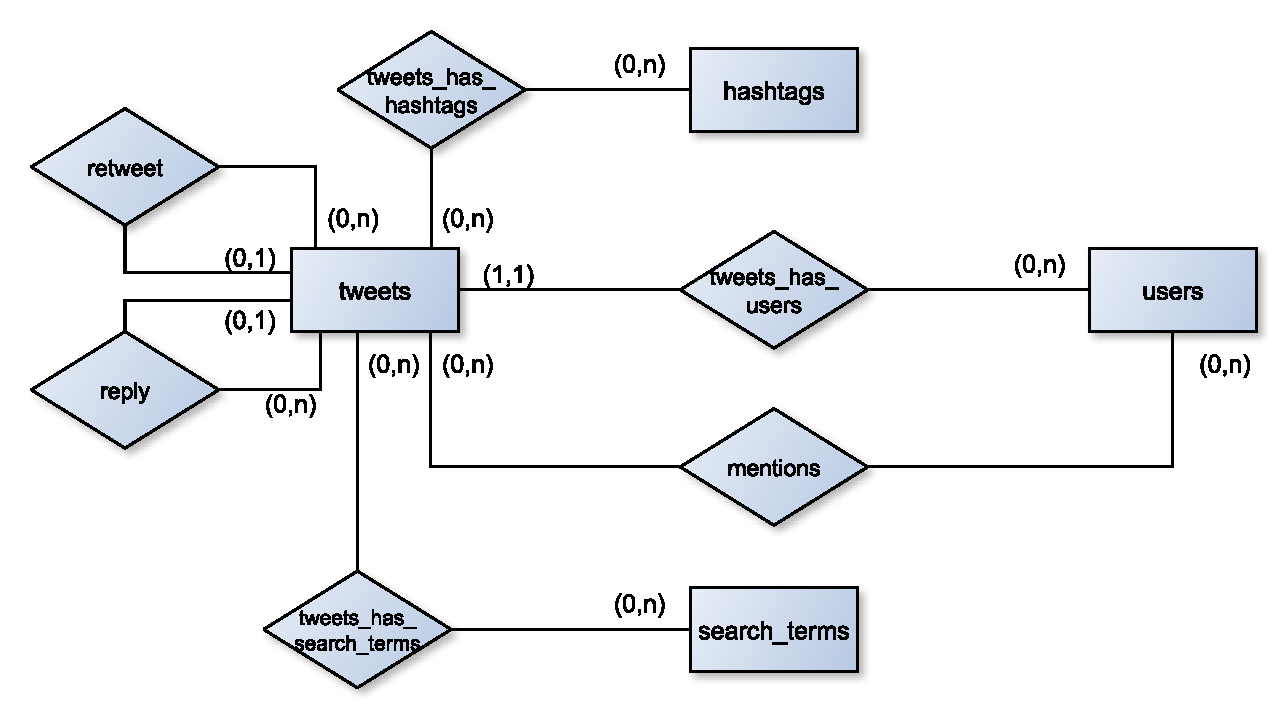
\includegraphics[width=\textwidth]{Bilder/Datenbank/ERM_Datenbank.pdf}
\caption{Bei Projektbeginn aufgestelltes Entity-Relationship-Modell}
\label{img:ERM_DB}
\end{figure}

Bei der Datenbankmodellierung wurde als erster Schritt ein Entity-Relationship-Modell aufgestellt.
Damit lassen sich die zu speichernden Twitter-Informationen zunächst auf einer konzeptionellen Ebene betrachten, die den Blick auf das Wesentliche lenkt.
Abbildung \ref{img:ERM_DB} zeigt das ER-Modell, welches zu Projektbeginn aufgestellt wurde und trotz späterer Datenbankänderungen nach wie vor die Grundstruktur zeigt.
Beispielsweise ist ein Tweet genau einem User zugeordnet, wobei ein User beliebig viele Tweets veröffentlichen kann.
Ebenso können in einem Tweet mehrere Nutzer erwähnt sein und andersherum kann ein Nutzer in mehreren Tweets erwähnt sein ($(0,n)-(0,n)$-Beziehung \texttt{mentions}).
Außerdem sind Retweets und Replies als Hierarchie modelliert, da hier eine Beziehung zwischen gleichen Entities entsteht, nämlich zwei Tweets.
Zum Beispiel bezieht sich ein Retweet immer auf einen Originaltweet, sodass einem Tweet maximal ein anderer übergeordnet werden darf.
Außerdem können einem Tweet beliebig viele Tweets untergeordnet werden (dessen Retweets).

Der einzige Entity-Typ, der sich dabei nicht direkt aus den Daten von Twitter ergibt, ist \texttt{search\_terms} mit dem Relationship-Typ \texttt{tweets\_has\_search\_terms}.
Der Entity-Typ \texttt{search\_terms} speichert die vom Nutzer eingegebenen Suchbegriffe, sowie später hinzugefügte Verwaltungsdaten für den Daemon.

Das ER-Modell wurde anschließend in ein relationales Datenbankschema überführt, welches mithilfe von MySQL Workbench erstellt wurde.
Dieses Programm erlaubt die direkte Generierung der SQL-Statements, um die entsprechende Datenbank zu erstellen. 
Den ersten Entwurf des Schemas zeigt Abbildung \ref{img:schemadb1}.

\begin{figure}[!ht]
\centering
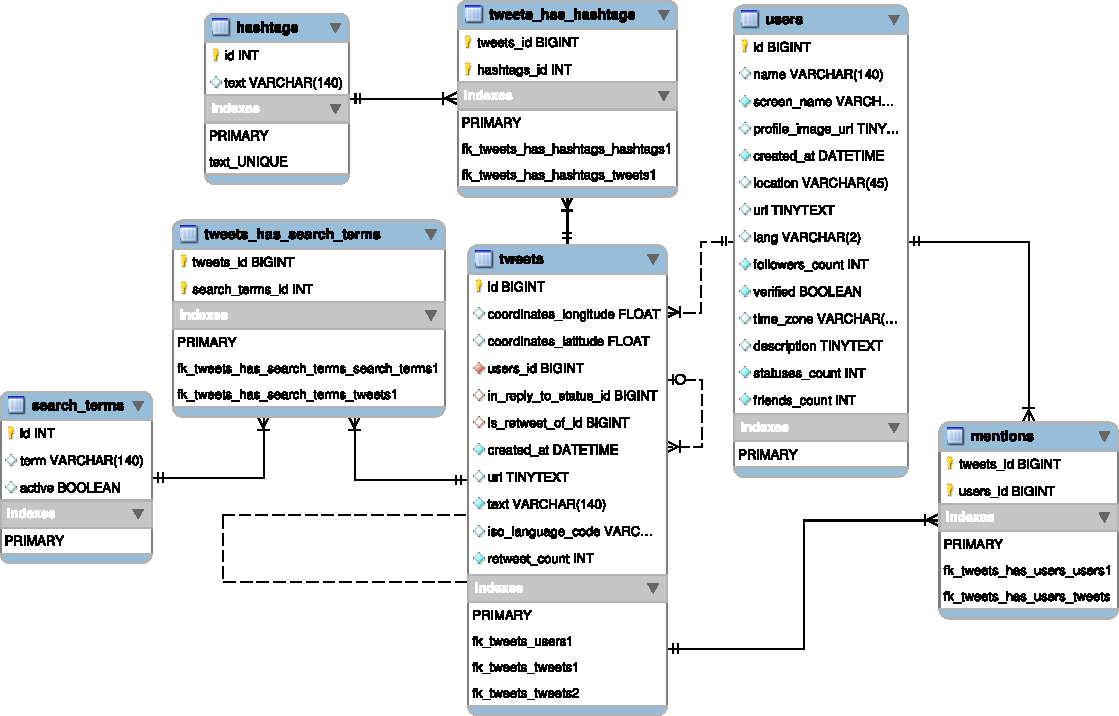
\includegraphics[width=0.9\textwidth]{Bilder/Datenbank/SchemaErsteIteration.pdf}
\caption{Erstes relationale Datenbankschema}
\label{img:schemadb1}
\end{figure}

Zum Beispiel ist zu erkennen, dass die Beziehung \texttt{tweets\_has\_users} im ER-Model nicht in einer eigenen Tabelle resultiert.
Stattdessen enthält die \texttt{tweets}-Tabelle eine zusätzliche Spalte \texttt{users\_id}, die als Fremdschlüssel auf die \texttt{users}-Tabelle referenziert.
Die beiden Hierarchien \texttt{retweet} und \texttt{reply} sind auf die gleiche Weise überführt worden.
Dagegen resultiert die \texttt{mentions}-Beziehung aufgrund der $(0,n)-(0,n)$ Kardinalitäten in einer eigenen Tabelle. 

\subsubsection{Anpassungen des Schema}
Im Verlauf der Iterationen gab es mehrere Änderungen am Schema.
So gab es zu Beginn Probleme mit der Länge einiger Felder, gerade das Feld für den Text der Tweets war zu kurz, da Twitter die Tweets als UTF-8 kodiert, MySQL aber für UTF-8 mehr als ein Zeichen benötigt.
Größere Änderungen brachte der Daemon mit sich. Dieser braucht verschiedene Verwaltungsdaten, die der \texttt{search\_terms} Tabelle hinzugefügt wurden.
Da die Menge der hinzugefügten Daten recht gering und auch die Anzahl der Einträge der Suchbegriffe insgesamt relativ gering ist, sind dadurch keine negativen Einflüsse auf die Performance zu erwarten.
%Außerdem gab es durchaus sich widersprechende Änderungen, da eine Funktionalität zuerst ausprobiert und dann wieder verworfen wurde.
In der letzten Iteration wurde noch eine Denormalisierung des Schemas aus Performance-Gründen eingeführt. 
Auf das Lösen der Performance-Probleme geht der nächste Abschnitt \ref{ssec:Performance} genauer ein.
Unser endgültiges Schema zeigt Abbildung \ref{img:schemadbfinal}.
\begin{figure}[ht]
\centering
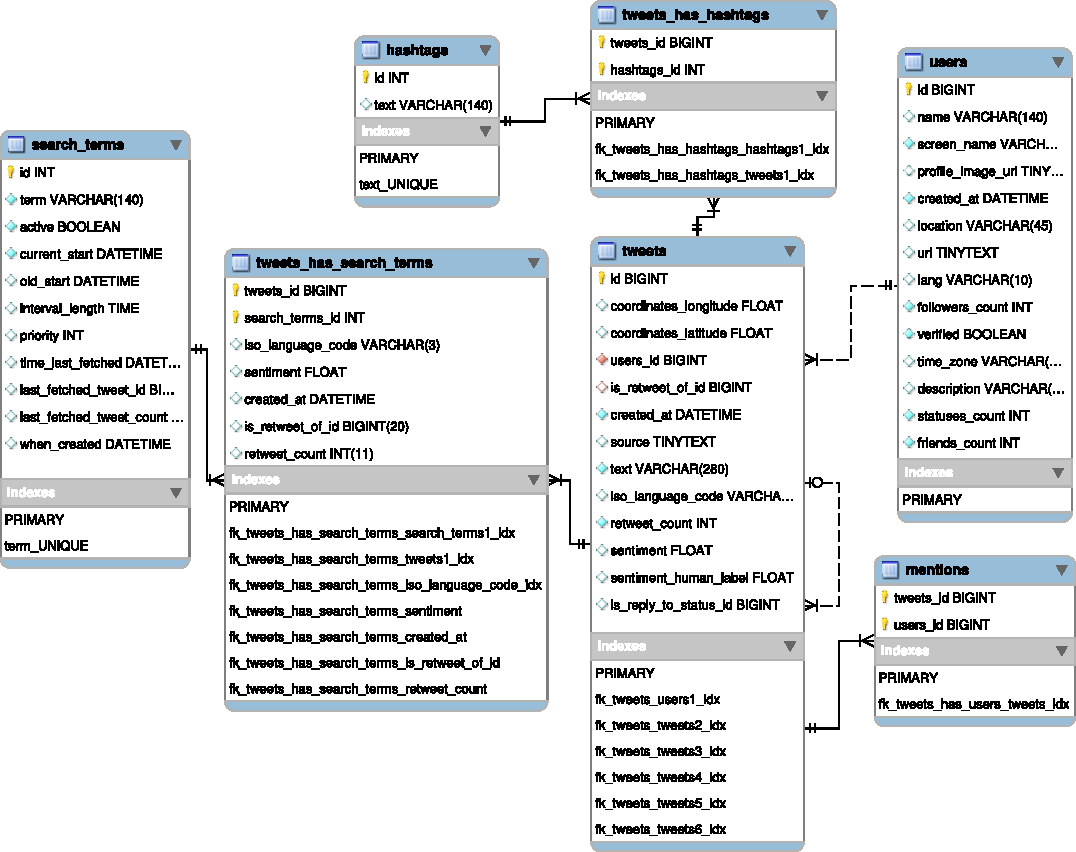
\includegraphics[width=0.8\textwidth]{Bilder/Datenbank/SchemaLetzteIteration.pdf}
\caption{Finales relationale Datenbankschema}
\label{img:schemadbfinal}
\end{figure}
Dabei ist zu sehen das die meisten Änderungen, im Vergleich zur ersten Version, an der \texttt{search\_terms}- und \texttt{tweets\_has\_search\_terms}-Tabelle stattgefunden haben.

\subsubsection{Probleme mit UTF-8}
%Gerade am Anfang gab es Probleme mit UTF-8.
Der Text von Tweets, aber auch Selbstbeschreibungen der User und andere Texte sind bei Twitter UTF-8-kodiert.
MySQL unterstützt zwar UTF-8, unterscheidet dabei aber zwei Versionen.
Die \texttt{utf8} genannte Version verwendet dabei nur 3 Byte pro Zeichen und unterstützt deswegen nicht den ganzen Umfang von UTF-8. Daher fehlen z.\,B. \textit{emoji} und weitere Zeichen, die mit 4 Byte kodiert werden.
Der bei MySQL \texttt{utf8mb4} genannte Zeichensatz verwendet hingegen 4 Byte pro Zeichen und ist deswegen in der Lage alle Zeichen von UTF-8 darzustellen.
Dieser Zeichensatz wird ab MySQL-Version 5.5 unterstützt, während frühere Versionen nur \texttt{utf8} unterstützen. Die Unterschiede werden auch in der MySQL-Dokumentation \cite{MySQLutf8} erläutert.
Da viele Tweets aus dem asiatischen Raum nicht vom \texttt{utf8}-Zeichensatz unterstütze Zeichen und viele \textit{emoji} enthalten, musste MySQL auf Version 5.5 aktualisiert werden und das Schema auf \texttt{utf8mb4} umgestellt werden.

\subsection{Performance}
\label{ssec:Performance}
Ein großes Thema für uns war die Performance der Datenbank.
Sobald der Daemon genug Tweets gesammelt hatte, stellte sich heraus, dass die Performance der Anwendung, insbesondere der Datenbank, nicht unseren Ansprüchen genügte.
Deshalb wurde das MySQL-\textit{Slow-Log} aktiviert, um langsame Abfragen zu identifizieren.
Dabei stellte sich heraus, dass ein großer Teil unserer Abfragen langsam war und nicht nur vereinzelte.
Problematisch war dabei nur die Ausführungszeit der Abfragen selbst, nicht die Zeit, in der \textit{locks} gehalten werden.

\subsubsection{Indizes}
Als erster Lösungsansatz wurde für jede Spalte separat untersucht, ob das Nutzen von Indizes sich positiv auf die Laufzeit der Abfrage, welche auf die entsprechende Spalte zugreift, auswirkt.
In einigen Fällen konnten so erhebliche Steigerungen festgestellt werden, sodass ein entsprechender Index für die Spalte angelegt wurde.
So gibt es zum Beispiel eine Abfrage, die einen Wert aus jeder Zeile aufsummiert, welche nicht vom Index profitiert.

\subsubsection{Unterabfragen}
Trotz der Indizierung einiger Spalten in der Datenbank hatten einige Abfragen noch eine sehr hohe Laufzeit. Der Grund dafür  sind die aufwändigen Joins der Tabellen. Damit weniger Datensätze in einem Join verbunden werden müssen, wurden Unterabfragen eingeführt. So wurden zum Beispiel vor dieser Veränderung zuerst alle Datensätze der \texttt{tweets}-Tabelle mit der \texttt{tweets\_has\_search\_terms} gejoint und danach erst die Einschränkungen im \texttt{where}-Teil der Abfrage ausgewertet. Eine Verwendung von Unterabfragen führt dazu, dass die Einschränkungen vor dem Join ausgewertet werden und nur die relevanten Datensätze mit der \texttt{tweets\_has\_search\_terms} verbunden werden. Dadurch wurde zum einen die Zeit verringert, die benötigt wird, um den Join durchzuführen. Ebenfalls wird der Speicherbedarf der Anfrage im RAM verringert.
Teilweise konnte dabei dennoch beobachtet werden, dass MySQL die temporären Tabellen auf die Festplatten auslagert, weil sie zu groß für das RAM waren.

%Grund war meistens, dass es sich um sehr große Tabellen handelte, weil es sehr viele Tweets zu einem Thema gab, oder noch besondere Operationen wie Sortieren auf den Daten ausgeführt werden mussten.
%In einigen Fällen war es möglich, die Abfragen selbst anzupassen um die Laufzeit zu verbessern.
%Gerade der Einsatz von Unterabfragen konnte die Laufzeit einiger Abfragen verbessern.

\subsubsection{Denormalisierung}
Um das Problem der zu großen Tabellen weiter zu lösen, wurde in der letzten Iteration beschlossen, das Schema zu denormalisieren und einige Werte, die ursprünglich ausschließlich in der \texttt{tweets}-Tabelle standen, in die \texttt{tweets\_has\_search\_terms}-Tabelle zu übernehmen. Hierdurch konnte der Join dieser beiden Tabellen in vielen Abfragen vermieden werden. Dies bewirkte eine weitere Verkleinerung der temporären Tabellen.
Die Änderungen sowohl an der Datenbank als auch an der Anwendung waren vergleichsweise klein und schnell umzusetzen und brachten an vielen Stellen bemerkbare Performanceverbesserungen.

%Ein weiteres Problem, das identifiziert werden konnte war, dass viele Queries mit hoher Laufzeit die mehrere Tabellen, insbesondere die Tweets-Tabelle, mit anderen gejoined haben.
%Da die Tweets-Tabelle die größte Tabelle ist, ist dies sehr langsam.
%Deswegen wurde unter dem Zeitdruck der letzten Iteration beschlossen, 


\subsubsection{Zählen, Sortieren und weiteres}
Aufgrund der Anforderungen der Auswertung, wie zum Beispiel vielen zeitlichen Verläufen, gibt es viele Abfragen, die Felder in den Tabellen zählen und teilweise auch sortieren müssen. Diese Funktionen von MySQL sind aber für die Anzahl an Datensätzen, die in unserer Datenbank vorliegen, ineffizient.
Um diesen Flaschenhals zu entfernen, müssten die entsprechenden Werte in einer separaten Tabelle gespeichert werden. Das Speichern dieser Werte müsste vom Daemon übernommen werden. Hierbei würde zum Beispiel die Anzahl der Tweets zu einem Suchbegriff inkrementell berechnet und abgespeichert. Da solche so genannten \textit{rollup}-Tabellen größere Veränderungen sowohl am Schema als auch am Daemon erfordert hätten, wurde aus Zeitgründen darauf verzichtet.

%In diesem Fall lassen sich die Abfragen nicht anpassen, ohne die ganze Auswertung anzupassen oder die aufsummierten Werte, z.B. in einer extra Tabelle, zwischenzuspeichern.

%Prinzipiell hätte eine Erweiterung des Schemas um eine oder mehrere Tabellen mit Metadaten, die in sehr kurzer Zeit abgefragt werden können, aber relativ großes Potential.
%Dafür hätte aber sowohl das Schema als auch die Anwendung so stark angepasst werden müssen, dass dafür die Zeit nicht reichte.

\subsubsection{Dirty Reads}
Ein weiteres Problem war, dass die Ausführungszeit der Abfragen stark abnimmt, sobald der Daemon Tweets in der Datenbank speichert.
Da die Abfragen immer erst warten, bis der Daemon die neuen Werte gespeichert hat, konnte dies die Ausführungszeit deutlich erhöhen.
Da die Abfrage selbst aber nicht auf die allerneusten Tweets angewiesen ist, zumal die Tweets, die der Daemon einspeichert ja zu ganzen anderen Suchbegriffen gehören können, wurden die sogenannten \textit{dirty reads} aktiviert.
Dabei kann eine Abfrage die Daten lesen, selbst wenn der Daemon momentan weitere Datensätze in die Tabelle schreibt. Dies kann dazu führen, dass die Abfragen nicht alle relevanten Datensätze zurückgeben.
Für den Großteil der Anfragen können wir mit diesen gegebenenfalls inkonsistenten Werten aber ohne Probleme arbeiten.
Diese Veränderung löst das Problem der Datenbankanfragen, die selbst eine lange Anfragezeit haben, allerdings nicht. Lediglich die Auswirkungen gleichzeitiger Schreibe- und Lese-Operationen können so gemindert werden.

\subsubsection{Fazit}
Die Datenbank hat im Laufe des Projektseminars mehrere Iterationen durchlaufen. 
Zum Ende des Projekts lässt sich zusammenfassen, dass die Performance weiter gesteigert werden muss, um insbesondere den Anforderungen einer Echtzeitanwendung gerecht zu werden. 
Die Veränderungen haben bereits deutliche 
Verbesserungen zur Folge gehabt.
Ein möglicher nächster Schritt wäre die weitere De- und anschließend erneute Normalisierung des Schemas, 
um zum Beispiel die oft abgefragten von den selten abgefragten Daten zu trennen, oder die Einführung 
der oben erwähnten \textit{rollup}-Tabellen für Metadaten, wie Summen von Tweets.
%Es gab einige Veränderungen, die teilweise deutliche Verbesserungen gebracht haben.
%Auch die Denormalisierung hat die Performance nochmal verbessert.
%Aber auch die Summe aller Verbesserungen war noch nicht so gut, dass man das Ganze als ein fertiges Produkt betrachten könnte.
%Das Verbessern der Performance ist also noch keineswegs abgeschlossen. 

%Entweder indem große, selten genutzte Daten, wie zum Beispiel der Text bei den Tweets, von kleinen oft benutzten Metadaten getrennt werden, in der Hoffnung das dies Hilft.
%Oder indem man, mit den jetzt konkreten Anforderungen und Abfragen, die Performance unterschiedlicher Datenbanksysteme nochmal vergleicht.
\section{REST}
\label{sec:rest}
\subsection{Einführung}
\label{resteinfuehrung}
Das Wort REST ist eine Abkürzung für \textit{Representational State Transfer} und bezeichnet ein Programmierparadigma speziell für Webanwendungen. Vorgeschlagen wurde es von Roy Fielding in seiner Dissertation aus dem Jahr 2000 \cite{fielding}. In einem Satz lässt sich das Paradigma wie folgt zusammenfassen: REST sieht vor, dass bei einer Anfrage an eine URL immer die gleichen Ressourcen vom Server zurückgeliefert werden. Das Programmierparadigma lässt sich am einfachsten anhand seiner Eigenschaften beschreiben.

\subsubsection{Client-Server}
Die Kommunikation zwischen dem Server und dem Webbrowser oder Client findet nicht direkt statt, sondern ist durch ein Interface getrennt. Dies bedeutet, dass die beiden Komponenten keinerlei Informationen über den Zustand des anderen benötigen und sich nicht um Implementierungsdetails der anderen Komponente kümmern müssen. Dies ermöglicht eine einfache Portierung der Client-Software über verschiedene Plattformen hinweg. Die Skalierbarkeit des Servers wird ebenfalls verbessert, da seine Komponenten vereinfacht werden können. Der größte Vorteil dieser Eigenschaft ist allerdings die Möglichkeit, Server und Client getrennt voneinander zu entwickeln, sofern vorher eine Schnittstelle definiert wurde.

\subsubsection{Zustandslosigkeit}
Eine zusätzliche Einschränkung, die zu der Client-Server Kommunikation hinzugefügt wird, ist die Bedingung, dass die Kommunikation zustandslos sein muss. Dies bedingt, dass alle relevanten Informationen für eine Anfrage an den Server in dieser enthalten sein müssen und die Session auf der Clientseite abgehandelt werden muss. Diese Bedingung verbessert ebenfalls die Skalierbarkeit, da zwischen den einzelnen Anfragen keine zusätzlichen Informationen gespeichert werden müssen. Weiterhin wird die Robustheit des Systems gestärkt, da ein Fehler innerhalb einer Anfragebearbeitung keine weiteren Anfragen beeinflusst.

\subsubsection{Cache}
Um die Ressourcen des Netzwerks optimal zu nutzen wird vorausgesetzt, dass Anfragen an den Server explizit als \textit{cacheable} markiert werden müssen. 

\subsubsection{Einheitliches Interface}
Die Interfaces, die die Kommunikation zwischen verschiedenen Komponenten des Programms abwickeln, müssen einheitlich sein. Hierdurch wird die allgemeine Systemarchitektur vereinfacht und die Kommunikation bleibt einheitlich.

\subsubsection{Schichten}
Die Struktur des Programms sollte in Schichten unterteilt sein, wobei keine Schicht mit einer anderen interagiert, die nicht ihre direkte Nachbarschicht ist. So ist es möglich, bestimmte Funktionen in einer Schicht zu gruppieren und dadurch die Komplexität des Programms weiter zu reduzieren.

Da unser Endprodukt eine Webanwendung für verschiedene Plattformen sein soll, erschien dem Team dieses Programmierparadigma als sinnvoller Ansatz für unsere Server-Architektur.


\subsection{Implementierung}

Zur Implementierung unseres REST-Services in Java verwenden wir Jersey \cite{Jersey}, die Standardbibliothek für Java-APIs für RESTful Services (JAX-RS). Jersey ermöglicht die Implementierung eines REST-Services innerhalb einer Java-Klasse, ohne die dabei notwendige HTML-Kommunikation explizit behandeln zu können. Wie bereits beschrieben, sind in einem REST-Service serverseitige Ressourcen definiert, mit denen ein Benutzer als Client über HTML-Anfragen an eine assoziierte URL interagieren kann.

Ein REST-Service funktioniert also immer in Reaktion auf eine Benutzer-Anfrage. Um diese Reaktion in Java implementieren zu können, kann in Jersey eine Ressource mit einer Java-Methode in Verbindung gesetzt werden. Das geschieht, indem für die Methode spezifiziert wird, welche Art von HTML-Anfrage auf welche URL zum Aufruf der Methode führt. Die URL setzt sich dabei aus den Einstellungen für die globale Basis-URL (welche gemeinsam mit anderen Einstellungen in einer \texttt{web.xml}-Datei festgelegt werden kann), dem URL-Bestandteil der Klasse und dem URL-Bestandteil der Methode zusammen. Die Bestandteile der Klasse und der Methode können dabei durch den Parameter der von Jersey bereitgestellten Annotation \texttt{@Path} definiert werden. Zusätzlich stehen außerdem Annotationen zur Verfügung, welche die Art der HTML-Anfrage spezifizieren, da jeweils unterschiedliche Methoden für ihre Ausführung notwendig sind. Von diesen haben wir ausschließlich \texttt{@GET} und \texttt{@POST} verwendet. Eine beispielhafte Verbindung der Methode \texttt{getTweets()} GET-Anfrage auf die URL \texttt{www.tmetrics.de/rest/tweets} (zusammengesetzt aus der Basis-URL \texttt{www.tmetrics.de} sowie den Bestandteilen \texttt{/rest} der Klasse und \texttt{/tweets} der Methode) ist in Abbildung \ref{jerseyurl} zu sehen.

\begin{figure}[h]
\centering
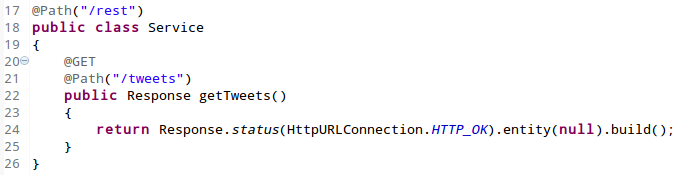
\includegraphics[scale=0.6]{Bilder/REST/JerseyURL.png}
\caption{Jersey: Verbindung von Methoden mit HTML-Anfragen}
\label{jerseyurl}
\end{figure}

Wie ebenfalls an der Abbildung erkennbar ist, liefert jede mit Jersey implementierte Methode eines REST-Servers standardmäßig eine HTML-Response zurück, welche durch die \texttt{Response}-Klasse repräsentiert wird. Die eigentlichen Antwortdaten können dabei als Bestandteil des Entity-Attributs der Response übergeben werden (in diesem Beispiel nur \texttt{null}). Dabei kann mit einer weiteren Annotation spezifiziert werden, in welcher Form die Daten in der Entity an das Frontend gesendet werden. Da das Frontend in JavaScript implementiert ist, haben wir uns hier für das auf JavaScript ausgerichtete JSON-Format entschieden. Dieses kann über den Parameter der Annotation \texttt{@Produces} spezifiziert werden (siehe Abbildung \ref{jerseyproduces}). Primitive Datentypen sowie in JavaScript vorhandene Datenstrukturen werden dabei automatisch geparst. Für eigene Klassen muss das Parsing explizit definiert werden (siehe Abschnitt \ref{sec:dto}). Dieses Parsing macht es sogar möglich, anstatt einer expliziten Response direkt die Daten zurückzugeben. Diese werden dann implizit in eine Response verpackt. Dieses Vorgehen wurde zeitweise von uns eingesetzt, aber im Projektverlauf verworfen, da uns eine explizite Kontrolle der Response insbesondere wegen der Statusnachricht als sinnvoll erschien.

\begin{figure}[h]
\centering
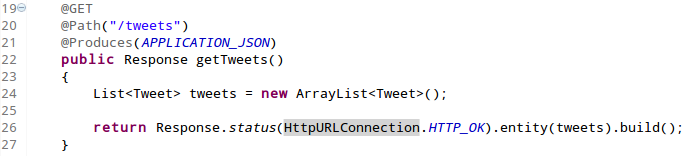
\includegraphics[scale=0.6]{Bilder/REST/JerseyProduces.png}
\caption{Jersey: Spezifizierung des Rückgabeformats}
\label{jerseyproduces}
\end{figure}

Häufig ist außerdem der Zugriff nur auf bestimmte Bestandteile einer Ressource notwendig. So ist niemals der gesamte Inhalt der Tweets-Ressource von Interesse, sondern nur die Tweets, die mit einem bestimmten Suchbegriff verbunden sind (welcher durch eine ID identifiziert wird). Es sind außerdem weitere Einschränkungen der Daten vorstellbar. So sind in bestimmten Ansichten nur Tweets aus einem bestimmtem Zeitraum oder mit einem bestimmten Sentiment von Interesse. Diese Parameter finden sich einerseits als Parameter in der URL der HTML-Anfrage und andererseits in der Signatur der entsprechenden Java-Methode wieder. Die Jersey-Annotation \texttt{@QueryParam} ermöglicht dabei die Verbindung eines Parameters der Anfrage mit einem Argument in der Methodensignatur. Dabei ist zu beachten, dass sämtliche Argumente \texttt{null} sind, falls ihnen entweder im Quellcode kein Anfrageparameter zugewiesen wurde oder falls die Anfrage diesen Parameter nicht beinhaltet. Soll also ein Parameter verpflichtend gemacht werden, muss diese Situation abgefangen und eine Exception geworfen werden. Eine Alternative bildet die Verwendung der Annotation \texttt{@DefaultValue}, womit ein Standardwert festgelegt wird, falls der Parameter nicht in der Anfrage vorkommt. Eine genauere Behandlung dieser Fälle wird in Abschnitt \ref{sec:serviceklassen} beschrieben. Auf ähnliche Weise können Methodenargumente über die Annotation \texttt{@HeaderParam} auch auf die Header-Parameter der HTML-Anfrage zugreifen. Diese Fälle werden in Abbildung \ref{jerseyparams} veranschaulicht. Ein valider Zugriff auf die in dieser Methode spezifizierte Ressource wäre beispielsweise eine GET-Anfrage auf \texttt{www.tmetrics.de/rest/tweets?id=1\&limit=100}. Aufgrund des Standardwertes könnte der \texttt{limit}-Parameter dabei auch weggelassen werden.

\begin{figure}[h]
\centering
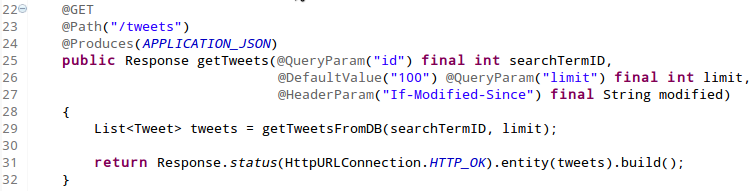
\includegraphics[scale=0.6]{Bilder/REST/JerseyParams.png}
\caption{Jersey: Übergabe von Parametern}
\label{jerseyparams}
\end{figure}

Auf diese Weise ermöglicht Jersey es, Java-Methoden mit HTML-Anfragen auf eine URL zu verknüpfen und die Eingaben und Ausgaben dieser Methode zu kontrollieren. Um eine konkrete HTML-Anfrage abzuhandeln, wird die Klasse, in der Jersey implementiert ist, neu instanziiert und die korrekte Methode identifiziert und ausgeführt. Diese neuerliche Instanziierung bei jeder Anfrage spiegelt die Tatsache wieder, dass ein REST-Service zustandslos ist.
\subsection{Struktur des REST-Service}

\subsubsection{Klassenstruktur}

Wie bereits erwähnt, ist die Aufgabe unseres REST-Service, eine Verbindung zwischen Benutzeranfragen und -eingaben auf der einen Seite und der Datenbank auf der anderen Seite herzustellen. Die Schnittstelle zur HTML-Kommunikation mit dem Benutzer bildet den REST-Service im engeren Sinne. Dieser wird bei uns von einer Klasse \texttt{Service} übernommen, in der wie zuvor beschrieben mit Jersey die REST-Schnittstelle implementiert wird. Die Kommunikation mit der Datenbank findet in der Klasse \texttt{Transactor} mittels JDBC statt.

Dabei gibt es jedoch keine direkte Kommunikation zwischen den Klassen \texttt{Service} und \texttt{Transactor}. Denn wie bereits in der Architekturübersicht dargestellt, besteht die Aufgabe des REST-Service im weiteren Sinne nicht nur in der Ausgabe von Daten aus der Datenbank, sondern auch aus deren Analyse. Zu diesem Analyseverfahren gehören das Clustering, die Identifikation von Peaks und die Darstellung von \textit{related news} sowie das Bestimmen von Einflussfaktoren des Sentiment-Wertes von Tweets. Damit diese Verfahren integriert werden können, befindet sich zwischen den \texttt{Service}- und \texttt{Transactor}-Klassen noch eine weitere Klasse \texttt{Logic}. Der Fluss der Daten sieht dabei folgendermaßen aus: eine REST-Anfrage des Benutzers ruft über Jersey die zugeordnete Methode der \texttt{Service}-Klasse auf. Diese Anfrage wird zunächst über die entsprechende Methode in \texttt{Logic} an eine \texttt{Transactor}-Methode weitergereicht, welche die benötigten Daten aus der Datenbank abruft. Diese werden dann an die \texttt{Logic}-Methode zurückgeliefert. Beinhaltet die Anfrage den Einsatz eines Analyseverfahrens, werden diese durch Einsatz der jeweils damit verbundenen Klassen an dieser Stelle durchgeführt. Wird beispielsweise das Clustering angefragt, liefert der \texttt{Transactor} eine entsprechende Auswahl Tweets, auf der dann in der \texttt{Logic}-Methode das Clustering durchgeführt wird.

Ein weiterer Aufgabenbereich der \texttt{Logic}-Klasse ist in einigen Fällen die Aufbereitung der vom \texttt{Transactor} zurückgelieferten Daten. Um beispielsweise den zeitlichen Verlauf der Aktivität oder des Meinungsbildes zu erhalten, werden von der Datenbank sämtliche Tweets nach der Stunde ihrer Erstellung gruppiert. Die Methode im Frontend, die diese Daten schlussendlich darstellen soll, erwartet dabei Paare aus Zeitpunkten und einer Anzahl in konstanten Intervallen. Da die Rückgabe der Datenbank die vollen Stunden, an denen gar keine Tweets erstellt wurden, gar nicht beinhaltet, müssen in der \texttt{Logic}-Klasse diese Zeitpunkte mit der Anzahl 0 nachträglich eingefügt werden.

Ist weder eine Analyse noch eine Aufbereitung der Daten notwendig, haben wir uns aus Gründen der Konsistenz der Implementierung entschieden, die \texttt{Logic}-Klasse nicht zu umgehen. In diesem Fall reicht sie die Ergebnisse einfach weiter.

Wie bereits im vorigen Kapitel angemerkt wurde, lassen sich mit Jersey sowohl Klassen als auch Methoden mit einem URL-Bestandteil versehen. Um eine semantische Trennung der REST-Anfragen zu gewährleisten, wurden auf diese Weise zwei REST-Service-Klassen implementiert. Die Klasse \texttt{ResultService} mit dem Pfadbestandteil \texttt{/results/} ist dabei für sämtliche Anfragen zuständig, welche mit den direkt für den Benutzer im Frontend sichtbaren Resultaten zu tun haben, d.\,h. den Inhalten der Views. Die Klasse \texttt{QueryService} mit dem Pfadbestandteil \texttt{/queries/} ist hingegen für alle übrigen internen Anfragen verantwortlich, wie zum Beispiel die Anfrage, ob ein spezifischer Suchbegriff bereits in der Datenbank vorhanden ist oder welche ID dieser hat. Analog dazu existieren die zwei \texttt{Logic}-Klassen \texttt{ResultLogic} und \texttt{QueryLogic}, welche allerdings weiterhin auf eine gemeinsame \texttt{Transactor}-Klasse zugreifen. Hintergrund dieser Trennung ist eine übersichtlichere Struktur sowohl der REST-API als auch des internen Java-Codes, welcher aufgrund der Vielzahl der Methoden ansonsten umständlich zu handhaben gewesen wäre.

\subsubsection{Data Transfer Objects}
\label{sec:dto}

Um die Kommunikation sowohl innerhalb des REST-Service als auch mit dem Frontend zu vereinfachen, haben wir uns für den Einsatz von \textit{Data Transfer Objects} (DTOs) entschieden. Dabei handelt es sich um ein \textit{Plain Old Java Object} (POJO), welches nur über private Felder sowie deren zugeordnete Getter und Setter verfügt. Da für gewöhnlich die Rückgabe einer Datenbankanfrage im Transactor sehr komplexe Daten mit einer großen Menge von Attributen zurückgibt, ist es sinnvoll, diese Daten in einem DTO zu kapseln, sodass sie leicht zu manipulieren sind und einfach zwischen Methoden verschickt werden können. Ein weiterer Vorteil ist, dass sich die DTOs unter Einsatz eines POJO-Mappers implizit ins JSON-Format parsen lassen, welches sich einfach in der JavaScript-Umgebung des Frontends verwenden und in Jersey als Rückgabetyp einer REST-Anfrage spezifizieren lässt.

Dies geschieht in unserem Projekt mithilfe der Bibliothek Jackson \cite{Jackson}. Diese stellt eine Reihe von Annotationen bereit, welche bei der Implementierung eines DTOs verwendet werden können, um festzulegen, wie dessen Attribute geparst werden sollen. Am wichtigsten sind dabei hier die Annotationen \texttt{@jsonproperty}, dessen Parameter festlegt, unter welchem Namen das Attribut im JSON geparst werden soll, sowie \texttt{@jsonignore}, das bestimmt, dass dieses Attribut beim Parsen ignoriert werden soll. Dabei können sämtliche primitiven Datentypen sowie alle Klassen, für die ebenfalls ein Jackson-Parsing definiert wurde, mit \texttt{@jsonproperty} versehen werden. Des Weiteren ist Jackson in der Lage, Arrays sowie Datenstrukturen mit direkter Entsprechung in JavaScript wie z.\,B. \texttt{List} oder \texttt{Map} in ihr JSON-Gegenstück zu parsen. Ein so über Jackson konfiguriertes DTO kann dann direkt im REST-Service als implizite HTML-Response an das Frontend zurückgeliefert werden, wo es im JSON-Format ankommt.

Auf diese Weise wurde für sämtliche Ressourcen ein geeignetes DTO implementiert. In einigen Fällen können dabei auch mehrere DTOs in einander geschachtelt sein. So sind zum Beispiel für die Darstellung eines Tweets im Frontend auch Informationen über den Benutzer notwendig, der diesen Tweet erstellt hat. Daher existiert ein DTO \texttt{TweetWithUser}, das wiederum die DTOs \texttt{Tweet} und \texttt{User} beinhaltet. Zusätzlich zu dieser Schachtelung von DTOs haben wir uns bei der Konzeption dafür entschieden, das Meta-DTO \texttt{Envelope} einzuführen, dass sämtliche anderen DTOs enthält. Der Vorteil eines solchen \texttt{Envelope} ist, dass es die Handhabung von Fehlern und anderem unerwarteten Verhalten ermöglicht. Zu diesem Zweck hat die Klasse neben dem Attribut \texttt{data} vom Typ \texttt{Object} zum Speichern des jeweiligen DTOs ebenfalls die Felder \texttt{status} und \texttt{error\_codes}. In \texttt{status} kann dabei der Erfolg der Operation abgespeichert werden (wobei in Anlehnung an HTML hauptsächlich \texttt{200 OK} für erfolgreiche Operationen und \texttt{500 Internal Server Error} für Fehler verwendet wurden), während \texttt{error\_codes} es ermöglicht, gegebenenfalls Informationen über die Fehlerursache wie z.\,B. die Stacktrace einer Exception zu hinterlegen. Da das \texttt{data}-Feld auch auf \texttt{null} belassen werden kann, kann in so einer Situation selbst dann ein Envelope zurückgeliefert werden, falls infolge eines Fehlers keine Daten vorliegen. Der Status sowie die Fehlernachricht ermöglichen dann das Abfangen von unerwartetem Verhalten im Frontend und erleichtern die anschließende Fehlerbehandlung.

Das Verpacken der DTOs geschieht dabei ebenfalls in der \texttt{Logic}-Klasse. Das bedeutet, dass das \texttt{ResultSet} der SQL-Anfrage im \texttt{Transactor} zunächst in einem DTO gekapselt wird, welches an die Methode in \texttt{Logic} übergeben wird. Unter Umständen geworfene Exceptions werden dabei ebenfalls zunächst unbehandelt weitergereicht. Wird in \texttt{Logic} eine Exception gefangen, liegen für gewöhnlich keine Daten vor, es wird dann ein \texttt{Envelope} mit negativem Status und der entsprechenden Stacktrace erstellt. Ansonsten wird das erhaltene DTO zusammen mit einem positiven Status in einen \texttt{Envelope} verpackt.

Die hier vorgestellte Struktur wird in Abbildung \ref{fig:reststruktur} visualisiert.

\begin{figure}[h]
\centering
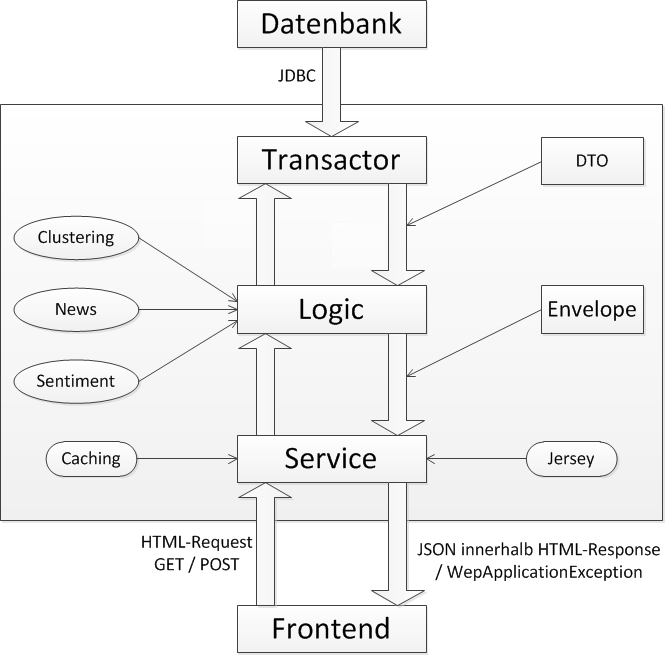
\includegraphics[width=0.6\textwidth]{Bilder/REST/RestServiceZeichnung.png}
\caption{Struktur des RestService}
\label{fig:reststruktur}
\end{figure}
\subsection{Umsetzung und Problemstellungen}
\label{sec:restUmsetzungen}
\subsubsection{Transactor}
Wie bereits oben beschrieben wird im \texttt{Transactor} die Verbindung zur Datenbank erstellt und die einzelnen Abfragen abgeschickt. Hierzu wird im Konstruktor der Klasse eine Verbindung zur Datenbank hergestellt. Die benötigten Parameter für die Verbindung werden aus einer \texttt{properties}-Datei geladen. Für jede Anfrage, die an den REST-Service gesendet wird, gibt es in dieser Klasse eine eigene Methode, die die SQL-Anfrage erstellt und abschickt. 

Die Anfragen werden mit Hilfe von \texttt{PreparedStatements} erstellt. Ein Anfragestring wird hierbei an den Konstruktor des \texttt{PreparedStatements} übergeben und die einzelnen Parameter mit einem Fragezeichen markiert. Die Werte für diese Parameter können dann im nächsten Schritt anhand eines Indexes gesetzt werden. Bei Anfragen, die optionale Parameter enthalten, müssen diese Anfragestrings dynamisch angepasst werden. Ein Problem, das dabei auftrat, sind die unterschiedlichen Indizes, die der gleiche Parameter bei unterschiedlichen Anzahlen von Anfrageparametern annehmen kann. Ein erster Ansatz dies zu lösen bestand darin, alle verschiedenen Kombinationen von gesetzten und nicht gesetzten Parametern durchzugehen und die Parameter für das \texttt{PreparedStatement} explizit zu setzen. Dies ist jedoch bereits ab einer kleinen Anzahl von Parametern nicht mehr praktikabel. Als sehr gute Lösung erwies es sich eine Laufvariable einzuführen, die nach jedem gesetzten Parameter um eins erhöht wird. So musste im Gegensatz zu allen Kombinationen von gesetzten und nicht gesetzten Parametern nur jeder einzelne Parameter überprüft werden. Sobald das \texttt{PreparedStatement} fertig gestellt ist, kann es an die Datenbank geschickt werden. 

Das Ergebnis der Anfrage liegt dann zuerst in einem \texttt{ResultSet} des \texttt{java.sql}-Packages vor. Diese \texttt{ResultSet}s werden dann direkt in die entsprechenden \textit{Data Transfer Objects} umgewandelt. Bei komplexeren DTOs wurden für diese Aufgabe Builder-Klassen implementiert, die das Befüllen der Objekte komfortabler machen.

In einer ersten Version des \texttt{Transactor}s wurden all diese Operationen in einem \texttt{try\-catch}-Block ausgeführt, um Exceptions, die bei dem Verbindungsaufbau mit der Datenbank oder beim Ausführen der Anfragen geworfen werden können, abzufangen. In dieser Version wurden die Fehlermeldungen direkt in den \texttt{Envelope} geschrieben und dieser zurückgegeben. Da diese Art der Fehlerbehandlung zu Problemen führte, wie im Unterkapitel zu den Service-Klassen näher beschrieben ist, werden die Exceptions in der aktuellen Version direkt weitergeworfen. Die \texttt{try-catch}-Struktur wurde in der \texttt{Transactor}-Klasse allerdings beibehalten, da dies einen \texttt{finally}-Block ermöglicht, in der sämtliche Verbindungen zur Datenbank definitiv geschlossen werden können. Dieses Kappen der Verbindungen ist sehr wichtig, um die Datenbank nicht mit zu vielen offenen Verbindungen zu blockieren.

\subsubsection{Logic-Klassen}
In den \texttt{Logic}-Klassen werden wie vorher beschrieben die Ergebnisse der Datenbankanfragen weiterverarbeitet. Neben den bisher beschriebenen Aufbereitungen werden hier auch die anderen Funktionen des REST-Service aufgerufen. Die Details der anderen Module, wie Clustern und der Newsanfrage, finden sich in den entsprechenden Komponenten-Kapiteln. 

Eine Besonderheit, die hier im Vordergrund stehen soll, ist die Einbindung der Daten für das Sentiment-Modell. Diese Informationen sind notwendig, um die Darstellung der Einflussfaktoren für die Sentimentanalyse eines Tweets zu ermöglichen. Da die Analyse im Daemon stattfindet und die Parameter, die zu dem Ergebnis geführt haben, nicht in der Datenbank vorgehalten werden, muss eine Möglichkeit gefunden werden, die Informationen auf einem anderen Weg in den REST-Service zu laden.

Die erste lauffähige Methode beinhaltete, die Sentiment-Klassen des Daemons in den REST-Service zu laden und die Analyse erneut für die aktuell angefragten Tweets durchlaufen zu lassen. Dies beinhaltet wegen der Zustandslosigkeit in jedem Aufruf ein neues Trainieren der Modelle. Diese Art der Redundanz erschien uns allerdings nicht haltbar. Die Methode, die uns das wiederholte Trainieren der Modelle abnahm, beinhaltete, die trainierten Modelle auf der Festplatte zu speichern und nach Bedarf im REST-Service zu laden. Die Modelle werden im Daemon trainiert und auf der Festplatte aktualisiert, sobald sich neue, von uns gelabelte Tweets, in der Datenbank befinden. Wie im 
%TODO Daemon oder senti
 Daemon-Kapitel beschrieben, wird der Thread, der diese Aktualisierung durchführt, einmal am Tag gestartet.
 
Die vorher beschriebene Eigenschaft der Zustandslosigkeit des REST-Service sorgte allerdings für ein weiteres Problem. Da aufgrund dieser Eigenschaft keine Informationen von einer Anfrage an den Rest-Service zur nächsten übertragen werden konnten, bedeutete dies, dass die Modelle für jede Anfrage neu geladen werden mussten. Bei etwa 5-6 MiB pro Modell und Sprache, bedeutet dieses Laden einen deutlichen Flaschenhals bei parallel laufenden Anfragen. Eine kleine Änderung der Klassenvariable für diese Modelle auf \texttt{static} sorgte dafür, dass die Modelle nur bei der ersten Anfrage geladen werden und danach weiterhin vorgehalten werden. Da unser Anspruch, möglichst präzise Informationen zu der Sentimentanalyse zu präsentieren, allerdings dadurch nicht mehr voll erfüllt wurde, musste eine Möglichkeit gefunden werden, die Modelle aktuell zu halten.

Der erste naive Ansatz hierzu war es, die Modelle im Speicher mithilfe einer Hashsumme mit den Modellen auf der Festplatte zu vergleichen. Da eine solche Summe allerdings erst dann für die Modelle auf der Festplatte berechnet werden kann, wenn diese in den Speicher geladen wurden, wurde diese Idee sehr schnell verworfen. Stattdessen wurde entschieden in den Modellen selbst ihre Erstellungszeit zu speichern. Diese Information ist sehr leicht auszulesen und konnte dann mit der Erstellungszeit der Dateien auf der Festplatte verglichen werden. Das Besondere bei dieser Methode ist, dass nicht die interne Erstellungszeit des Modells auf der Festplatte als Vergleichswert herangezogen wird, sondern der Zeitstempel im Dateisystem für die Datei. Sollte der Unterschied zwischen diesen beiden Zeitstempeln einen bestimmten Wert überschreiten, so ist das aktuelle Modell veraltet und wird neu geladen. Hierdurch konnte die zu ladende Menge an Daten pro Anfrage drastisch reduziert werden.

Da so ein akzeptabler Weg gefunden ist, die trainierten Modelle zwischen dem Daemon und dem REST-Service auszutauschen, können sowohl die Einflüsse für das Ergebnis der Sentimentanalyse, als auch die wichtigen Trainings-Tweets, die zu diesem Ergebnis geführt haben, ermittelt werden und an die nächste Schicht im REST-Service, die Serviceklassen, weitergeleitet werden.

\subsubsection{Service-Klassen}
\label{sec:serviceklassen}
Die \texttt{Service}-Klassen handeln, wie vorher beschrieben, die Kommunikation in Richtung Frontend ab. Neben dieser Kommunikation werden in diesen Klassen ebenfalls die Antworten erstellt, die dann endgültig an das Frontend geschickt werden. Der oben erwähnte \texttt{Envelope} wurde in einer früheren Version unseres Programms hier endgültig befüllt oder eventuelle Exceptions gefangen und in die entsprechenden Felder im \texttt{Envelope} geschrieben. Diese Informationen beinhalteten den Stacktrace und den Error-Code der gefangenen Exception. Ebenso wurden Informationen zu fehlenden oder fehlerhaften Anfrageparametern hier in einen Envelope geschrieben und an das Frontend weitergeleitet.  

Diese Herangehensweise an die Fehlerbehandlung hatte allerdings einen großen Nachteil. Der HTTP-Status-Code der Antwort des REST-Service war bei dieser Implementierung immer \texttt{200 OK}, egal ob ein Fehler im Programm vorlag, ein Parameter fehlerhaft war, oder die Anfrage ohne Probleme durchgelaufen war. Dies bedeutete, dass im Frontend zur Behandlung nicht vorhergesehener Fehler neben dem HTTP-Status der Antwort auch die internen Felder des \texttt{Envelope}s überprüft werden mussten. Um diese doppelte Überprüfung zu eliminieren wurde festgelegt, dass die HTTP-Status-Codes abgefangene Fehler im Programmcode widerspiegeln sollten. Hierzu wurden die Methoden der Klasse so umgeschrieben, dass sie nun explizit eine HTTP-Response zurückgaben. Die bisherigen \texttt{Envelope}s wurden dann als \texttt{entity} in diesen \texttt{Response}-Objekten gespeichert.

Diese Änderung ermöglichte es ebenfalls, \texttt{WebApplicationException}s für die Fehlerbehandlung zu benutzten. Eventuell geworfene Exceptions in einer tieferen Schicht des REST-Service werden nun hier gefangen und als \texttt{WebApplicationException} an das Frontend weitergereicht. Da diese \texttt{WebApplicationException} ebenfalls über ein HTTP-Response-Objekt an das Frontend weitergegeben wird, kann erneut der \texttt{Envelope} als \texttt{entity} gesetzt werden. Das bedeutet, dass der HTTP-Status-Code \texttt{500 Internal Server Error} einen Fehler anzeigt, aber die wichtigen Informationen über die Art des Fehlers dennoch am Frontend auslesbar sind. Diese Informationen waren in Entwicklungsprozess sehr hilfreich, da ein Fehler, der bei der Entwicklung des Frontends auftrat, mit sehr genauen Informationen an die Entwickler des REST-Service weitergeleitet werden konnte. 

Die Behandlung fehlerhafter Parameter wurde ebenfalls deutlich erleichtert. Das Protokoll der HTTP-Status-Codes beinhaltet einen speziellen Code, um anzuzeigen, dass die Anfrage an den Server fehlerhaft war: \texttt{400 Bad Request}. Dieser Code konnte nun verwendet werden, um anzuzeigen, dass notwendige Parameter fehlten oder Parameter einen ungültigen Wert hatten.

Ein weiteres Feature, das durch diese Änderung ermöglicht wurde, ist das Caching der Ergebnisse im Browser. Hierzu wurde eine zusätzliche Methode in die unteren beiden Schichten des REST-Service eingefügt, die überprüft, wann das letzte mal für einen bestimmten Suchbegrif neue Daten von Twitter abgefragt wurden. Fragt ein Browser zum ersten mal nach der aktuellen Ressource, wird diese Information zusätzlich im Header der HTTP-Response unter dem Feld \texttt{Last-modified} gespeichert. Diese Information wird bei einer erneuten Anfrage an die gleiche Ressource erneut im Header mitgeschickt und kann dann zu Beginn der Methode ausgelesen und mit dem erneut aus der Datenbank abgefragten Zeitstempel verglichen werden. Handelt es sich um den gleichen Zeitstempel, so genügt es eine HTTP-Response mit dem HTTP-Status-Code \texttt{304 Not\_Modified} an den Browser zurückzusenden. Dieser verwendet dann zur Anzeige die in der letzten Anfrage erhaltenen Daten. 

Diese Methode erspart die komplexen Datenbankanfragen, wenn sich der unterliegende Datensatz nicht geändert hat, und ersetzt sie durch eine einfache Anfrage, die über einen Primärschlüssel abgehandelt werden kann.
%\section{Server}
\section{Server}
\subsection{Anforderungen und Grundsteine}
Nachdem die ersten allgemeinen Anforderungen an das Projekt durch das Projektteam festgelegt wurden, ergaben sich daraus ebenfalls die ersten konkreten Anforderungen an den nötigen technischen Unterbau. Da jedoch noch nicht alle Anforderungen bis ins Detail ausgearbeitet waren, wurden einige Punkte umgesetzt, die sich letztendlich nicht als zwingend notwendig erwiesen haben. Im folgenden Abschnitt werden die Details der Services auf dem Server und die generelle technische Umgebung beschrieben.

Aufgrund des allgemeinen Wunsches, laufende Services so weit wie möglich frei konfigurieren zu können, um z.\,B. Datenbank, HTTP, Mail und weitere Server flexibel an evtl. wechselnde Anforderungen anpassen zu können, war schnell klar, dass ein voller root-Zugang definitiv von Vorteil, wenn nicht unabdingbar wäre. Ein freier root-Zugang versprach ebenfalls schnelle Reaktionen und somit die Vermeidung von unnötigen Wartezeiten und Nachfragen bei der IVV (Informations-Verarbeitungs-Versorgungseinheit des Fachbereiches).

Erste Erkundigungen bei der IVV ergaben jedoch schnell, dass die Möglichkeiten hier stark eingeschränkt sein würden, sodass die Alternative, einen unabhängigen Server durch einen externen Anbieter zu mieten, auf der Hand lag. Die Wahl fiel auf den kleinsten vServer des Anbieters Server4You. Da die Leistungswerte bezüglich RAM und CPU des virtuellen Servers mindestens denen eines durch die IVV zur Verfügung gestellten Rechners entsprachen, war damit der erste technische Grundstein des Servers festgelegt.
Der zweite Grundstein bestand aus der Wahl des Betriebssystems. Zur Verfügung standen CentOS 6, Debian 6 und Ubuntu 10.04 LTS, jeweils in einer minimalen Variante und einer mit einem Hosting-Tool ausgestatteten.
Obwohl sowohl CentOS 6 als auch Debian 6 neueren Datums sind als Ubuntu 10.04 LTS, machten im Team vorherrschende Kenntnisse über Ubuntu diese Wahl ebenfalls relativ einfach. Da keinerlei Erfahrung mit dem gegebenem Hosting-Tool (Plesk) im Team vorhanden war und wir hier nicht künstlich in den Möglichkeiten eingeschränkt werden wollten, fiel die Wahl auf Ubuntu 10.04 LTS in der minimalen Variante.

Ein erster Überblick über die gegebenen Anforderungen schien nicht gegen Ubuntu 10.04 LTS zu sprechen, da für alle relevanten Systemdienste wie z.\,B. Tomcat, Apache und MySQL in genügend aktuellen Versionen vorzuliegen schienen.
Im Ergebnis kann aber festgehalten werden, dass Ubuntu für unser Team definitiv die richtige Wahl war, da hier keinerlei weitere Einarbeitungszeiten nötig wurden und alle Teammitglieder selbständig und ohne Probleme mit dem System arbeiten konnten.

Da zu diesem Zeitpunkt noch nicht endgültig feststand, wie der Funktionsumfang unseres Projektes exakt aussehen wird, standen noch einige Punkte wie eine Benutzerverwaltung oder Zugänge im Raum, welche im weiteren Verlauf jedoch an Bedeutung verloren. Dies war zunächst jedoch ein weiteres Argument für einen unabhängigen Server, denn nur so war es möglich, ohne große Aufwände ein eigenes und kostenloses Zertifikat zu integrieren um so die verschlüsselte Verbindung zwischen Browser und Server zu gewährleisten. Dies sollte sich im weiteren Verlauf dennoch als ein durchaus nützlicher Pluspunkt herausstellen.
Um evtl benötigte Mailadressen für eine Registrierung bei Twitter zur Verfügung zu haben, wurde die Idee begrüßt einen eigenen Mailserver zu betreiben.

\subsection{Projektname und Grundkonfiguration}
Nachdem die Basis des Servers nun also gegeben war, bestand der nächste Schritt darin, die einzelnen Services zu installieren, konfigurieren und unseren Anforderungen anzupassen.
Um den Server über einen Namen ansprechen zu können, legte sich das Team relativ schnell zunächst auf \texttt{twittermetrics} und später dann auf \texttt{tmetrics.de} fest. Der Grund für diesen Wechsel war, dass wir über den Anbieter StartSSL.com kein Zertifikat erhalten konnten, welches einen Markennamen wie z.\,B. Twitter im Domainnamen enthält. Daher wurde im allgemeinen Konsens der Name tmetrics gewählt. Dieser ließ den zusätzlichen Interpretationsspielraum, dass man das t sowohl für Twitter als auch für Trend stehen könne.

Damit war der Einstiegspunkt für die Konfiguration des Webservers gegeben. Nachdem im Rahmen der allgemeinen Projekt Anforderungen schnell klar wurde, dass Java als zentrale Programmiersprache zum Einsatz kommen sollte, wurde ein Server benötigt, welcher Java Programme nativ zur Beantwortung der Browser-Requests ausführen kann. Aufgrund vorhandener Erfahrung mit den Produkten der Apache Software Foundation lag die Wahl eines Tomcat als Application Server sehr nahe. Weitere Alternativen wie Jetty oder der sehr mächtige WebSphere von IBM wurden daher nicht weiter untersucht.
Obwohl der Tomcat durchaus in der Lage ist statischen Content wie z.\,B. HTML, CSS und JavaScript auszuliefern, wurde für diesen Teil auf einen klassischen Apache Webserver gebaut.
Nebst dem Grund, dass der Apache bei der Auslieferung statischen Contents im Allgemeinen etwas schneller ist als der Tomcat, war auch hier wieder der im Team vorherrschende Erfahrungsschatz ein ausschlaggebendes Kriterium. Hier standen sich nur grundsätzlich vorhandene Erfahrungen der Konfiguration eines Tomcat mit tiefer gehenden und langjährigen Erfahrungen im Umgang mit dem Apache gegenüber.

Die Konfiguration entsprechender vHosts für den Domainnamen und Subdomains, der entsprechenden Einstellung für eine bestmögliche Verschlüsselung und die Einrichtung einiger Umleitungen um lediglich den Zugriff mittels HTTPS zu gestatten, stellten daher keine größere Herausforderung dar.

Interessanter war jedoch die Verbindung des Tomcat mit dem Apache. Da der Tomcat als eigenständiger Server auf unabhängigen Ports läuft, wäre es möglich gewesen, relativ einfach mittels des Apache-Proxy-Moduls \texttt{mod\_proxy} die Anfragen, welche an einen bestimmten externen Pfad gerichtet sind, intern auf den HTTP-Port des Tomcat umzuschreiben. 
Das Modul \texttt{mod\_jk} ermöglicht jedoch die Kommunikation über das \texttt{Apache JServ Protocol} (AJP) und somit eine deutlich tiefer gehende Kommunikation zwischen Application- und Web-Server. Von einfachen Diagnosemöglichkeiten, wie einer Kontrolle durch anpingen ob der Applicationserver noch läuft, bishin zu Anforderungen an Loadbalancing bietet AJP somit deutliche Vorteile gegenüber dem naiven Ansatz mittels HTTP-Proxy und wurde daher hier eingesetzt.
Nachdem der Tomcat erfolgreich mit dem Apache verbunden werden konnte, wurden alle externen Zugriffsmöglichkeiten abgeschaltet, sodass der Tomcat nur noch via AJP über den Apache zu erreichen ist.

Um während des Entwicklungsprozesses stets eine nicht zwingend vollständig fehlerfreie Testumgebung, parallel aber auch immer eine funktionsfähige Produktivversion zur Verfügung zu haben, wurden hierzu die Subdomains \texttt{www.} und \texttt{dev.} eingerichtet. Hierzu wurde der REST Service unter zwei verschiedenen Pfaden auf den Tomcat deployed. Unterhalb der URL \url{www.tmetrics.de/rest} stand der REST Service somit nativ zur Verfügung. Hinter der URL \url{dev.tmetrics.de/rest} verbarg sich jedoch zunächst ein Reverse-Proxy, welcher die Anfragen an \url{www.tmetrics.de/rest_dev} umgeleitet hat. Der statische Content unterhalb dieser beiden Domains wurde einfach aus zwei verschiedenen Verzeichnissen geliefert.

Die nächste Anforderung bestand darin, die fertig kompilierten REST-Projekte auf den Tomcat zu deployen. Hierzu wird einfach auf die Tomcat eigene Manageroberfläche zurückgegriffen. Damit lässt sich eine .war Datei einfach hochladen und auf einen bestimmten Pfad deployen. Dies stellte im Gegensatz zum Einbinden via Dateisystem und anschließendem Reload des Tomcat die einfachere und damit bevorzugte Möglichkeit gar.

Normalerweise ist der Zugang zu der Management-Konsole lediglich über ein Passwort mittels des \textit{Basic Auth} Verfahrens gesichert, was ohne eine sichere Verbindung über HTTPS ein gewisses Sicherheitsrisiko geboten hätte, da das Passwort in jedem Request des Browsers mitgeschickt wird und somit ohne große Mühen von potentiellen Angreifern hätte ausgelesen werden können.
Da wir bereits eine gesicherte Verbindung einsetzen und die Management-Konsole wie alle anderen Tomcat-Applikationen über den Apache ausgeliefert werden, bestand an dieser Stelle kein weiterer Handlungsbedarf und die Konfiguration des Tomcat war somit abgeschlossen.

Von den vorhandenen Zertifikaten profitierte ebenfalls die Einrichtung der Mailserver. So konnten sowohl der SMTP-Server \texttt{postfix} als auch der IMAP- und POP-Server \texttt{dovecot} problemlos für verschlüsselte Verbindungen eingerichtet werden. Die Webmail-Anwendung \texttt{SquirrelMail} (\url{https://mail.tmetrics.de}) nutzt zur Beschleunigung der Zugriffe noch das \texttt{imapproxy} Paket. Somit konnte zur Registrierung der verschiedenen Twitter-Accounts, die für die Minions notwendig waren bequem über bekannte lokale Clients oder ein Webinterface gearbeitet werden.

Als letzter Service sei an dieser Stelle der MySQL-Server und dessen Konfiguration erwähnt. Das reine Installieren des MySQL-Servers ging wie auch bei dem Tomcat und Apache über einen Shell-Aufruf nicht hinaus, und auch die weitere Konfiguration des MySQL-Servers hielt sich zunächst in Grenzen.
Aus Sicherheitsgründen wurde der Zugang von außen komplett blockiert, sodass nur von localhost aus auf den MySQL-Server zugegriffen werden konnte.
Diese Einstellung wurde im Laufe des Seminars verworfen, da es zu Testzwecken nötig wurde auch von außen Zugriff auf den MySQL-Server zu erhalten.

Da bei der ursprünglichen Konfiguration des MySQL-Servers aber auf die Einrichtung einer Verschlüsselung verzichtet wurde, wurde eine minimale Sicherheit der Datenbank durch unterschiedliche Benutzer umgesetzt. Nicht alle Datenbankbenutzer haben also von außen Zugriff auf die Datenbanken und jene, welche externen Zugriff haben, können nicht alle Daten verändern.
Der Verzicht auf eine verschlüsselte Datenbank-Verbindung war von verschiedenen Gründen getrieben. Zum einen sollten unnötige Performance-Einbußen vermieden werden, zum anderen konnte so ein potentieller \textit{point of failure} der Verbindung von Java zur Datenbank konsequent vermieden werden. Zumal nach anfänglicher Planung im späteren Produktivbetrieb sowieso wieder nur lokale Zugriffe stattfinden würden, wurde weiterer Aufwand an dieser Stelle für unnötig erachtet.

%TODO: Technik des Deamons beschreiben? Aber wie, ist ja nur ne JVM, eigentlich nix besonderes... Ist evtl hinreichend über den Architekturteil abgedeckt. - kannst ja nochmal im Architekturteil lesen ob dir das passt (und wenn nicht vielleicht da eher umschreiben, war mir selber nicht so sicher). Ist ja nichts aufregendes was man hier noch groß erwähnen muss - Andreas: ich lass es erstmal noch als Reminder hier stehen, sollte aber eigentlich passen.

Die Grundkonfiguration des Servers war somit gegeben und der Programmierarbeit stand nichts mehr im Wege.


\subsection{Ubuntu-Update auf virtuellem System}
Während die meisten Serverkomponenten so mehr oder weniger in ihrer endgültigen Konfiguration vorlagen, ergab sich in Bezug auf den MySQL-Server in den ersten zwei Wochen des Projektes bereits größerer Änderungsbedarf.

Um keine der durch Twitter gelieferten Information zu verlieren war es notwendig, mindestens die Tweets in dem Zeichensatz \texttt{utf8mb4\_general\_ci} zu speichern. Diese 4 Byte lange UTF8-Multibyte-Variante wurde von der eingesetzten MySQL-Version jedoch leider nicht unterstützt.%TODO Quell-Link?
Da auf der gegebenen Ubuntuversion keine neuere MySQL-Version verfügbar war, wurde somit ein Upgrade der Ubuntuversion notwendig.
Die Erwartungen, dass das Update eines Ubuntu-Systems so reibungslos funktioniert, wie man es von seinem privaten Computer gewohnt ist, wurden jedoch schnell zerstreut.
Nebst einiger konfigurationsbedingter Fehlermeldungen ließen sich einige kernelbezogene Fehlermeldung nicht ausmerzen. Eine daraufhin an den Server4You-Support gerichtete Nachfrage ergab, dass die virtuellen Systeme einen gemeinsamen Kernel einsetzen und dass dieser \textit{shared kernel} eben nicht mit Ubuntu 12.04 LTS kompatibel sei. Man wolle unseren vServer aber auf einen anderen \textit{shared host} umziehen, sodass ein Upgrade rein prinzipiell möglich sein sollte.
Da sich vor allem im Bereich der Mailserver-Konfiguration die Strutkur der Konfigurationsdateien nahezu vollständig geändert hatte, lief der erste Versuch auch mit neuerem \textit{shared kernel} nicht fehlerfrei durch.
Die aus den Fehlversuchen gewonnen Erfahrungen trugen jedoch dazu bei, dass der zweite Versuch mit dem neuen Kernel von Erfolg gekrönt war, sodass nach einigem Anpassen diverser Konfigurationsdateien endlich die neue Ubuntuversion fehlerfrei lief und somit auch die neue MySQL-Version inklusive der benötigten Kollation angeboten werden konnte.

Das Update der Ubuntuversion brachte nebst neuen Versionen an nahezu allen Serverkomponenten ebenfalls neue Versionen von Apache und OpenSSL mit sich. Die neuere Version der OpenSSL Bibliothek bot damit die Möglichkeit TLS v1.2 einzusetzen, womit die Sicherheit der HTTPS-Verschlüsselung letztendlich über das durchschnittliche Niveau der deutschen Onlinebanking-Anbieter gebracht werden konnte.

Ein weiterer Vorteil durch die Verwendung einer neueren Apache-Version ergab sich im Zusammenhang mit der Verwendung des von Google zur Verfügung gestellten Apache-Moduls \texttt{mod\_spdy}. Dies setzt als Mindestanforderung an den Apache die nun zur Verfügung stehende Version voraus.

\subsection{Performance-Optimierungen\label{sec:performance_opt}}
Da sich im Rahmen der Frontend Entwicklung ein Problem mit der durchschnittlichen maximalen Anzahl paralleler Verbindungen, die ein Browser zu einem Webserver offen halten kann, ergab, wurde versucht dieses Problem serverseitig durch die Verwendung des \texttt{mod\_spdy} zu beheben.
Das SPDY-Apache-Modul verspricht durch den Aufbau lediglich einer echten TCP-Verbindung zwischen Browser und Server die Performance durch Reduzierung des mehrfachen TLS-Handshake zu steigern. Dieses Modul dient der Erweiterung des HTTP-Protokolls bzw. der Einführung des SPDY-Prokokolls. Das Modul wird wird von Google implementiert und zur Verfügung gestellt, wobei das SPDY-Protokoll mittlerweile von den meisten gängigen Browsern unterstützt wird. Desweiteren dient das SPDY-Protokoll bzw. einige hier eingesetzte Techniken als Vorlage für die aktuell in den entsprechenden Gremien zur Abstimmung befindliche HTTP 2.0 Protokollversion.
Beim Einsatz des HTTP-Protokolls in der üblichen Version 1.1 muss für jede Ressource eine eigene Anfrage an den Server gestellt werden und somit jedes mal eine neue verschlüsselte Verbindung ausgehandelt werden. Das SPDY-Protokoll bündelt diese Anfragen innerhalb einer einzigen gesicherten TCP-Verbindung. Zunächst schien dies die Lösung zu sein, mehrere "'logische"' und vor allem parallele Anfragen als gewohnt anbieten zu können. Diese Annahme stellte sich jedoch als Fehler heraus. Tests ergaben, dass auch mit \texttt{mod\_spdy} nicht mehr parallel logische Verbindungen möglich waren als zuvor.
Somit war für unser System an dieser Stelle lediglich in Bezug auf die Auslieferung des statischen Content ein Performance-Vorteil vorhanden. Wir haben uns dennoch dafür entschieden, weiterhin \texttt{mod\_spdy} zu verwenden. Browser die dieses Protokoll nicht unterstützen fallen transparent auf HTTP(S) 1.1 (bzw. 1.0) zurück. 

Aufgrund von Problemen mit der parallelen Verarbeitung von PHP-Skripten im Zusammenhang mit \texttt{mod\_spdy} lief das eingesetzte \texttt{phpMyAdmin} nicht mehr, sodass für das PHP-Parsing noch ein \texttt{fgci}-Modul eingesetzt wurde. Nach der Installation der relevanten Apache-Module \texttt{libapache2-mod-fcgid} und \texttt{php5-cgi} und dem setzen des \texttt{fgci}-Handlers für \texttt{.php}-Dateien war aber auch dieses Problem behoben.

Da gegen Ende des Seminars die Performance von Datenbankoperationen nach und nach abnahm, nutzten wir einen kostenlosen Probemonat eines leistungsstärkeren dedizierten Servers. Eine Verbesserung bei der Datenbank und beim Daemon konnte festgestellt werden. Leider beseitigte das dennoch nicht alle Performance-Probleme, sodass das Team an dieser Stelle feststellte, dass eine Überarbeitung des Datenbankschemas wohl viel versprechender wäre als eine reine Leistungssteigerung der Hardware.

Um während der Präsentation dennoch ein einigermaßen performantes System zur Verfügung zu haben, wurden sämtliche Anfragen an den REST-Service mittels des Apache-Proxy-Moduls zwischengespeichert. Hierzu wurde der Aufruf des Rest Services auf einen anderen Pfad umgelegt (\url{www.tmetrics.de/rest_prod}) und auf dem alten Pfad (\url{www.tmetrics.de/rest}) ein Reverse-Proxy eingesetzt.
Nach einigen Untersuchungen in Bezug auf die verschiedenen Caching-Möglichkeiten, stellte sich heraus, dass leider nicht alles wie gewünscht gecached werden kann, da in den Anfrage URLs Query-Parameter wie z.\,B. \texttt{id=1} verwendet werden. Daher musste am REST-Service eine kleine Änderung vorgenommen werden, sodass alle Antworten nun mit einem Expires-Header ausgesendet werden. Dies hat zur Folge, dass alle Antworten des REST-Service sowohl im Browser als auch auf dem Proxy für 90 Minuten zwischengespeichert werden.
Im Zusammenhang mit dem Proxy ergibt sich also die Situation, dass sobald ein Besucher sich einmal die Auswertung für z.\,B. Merkel hat anzeigen lassen, diese direkt und unmittelbar auch für alle anderen Besucher zur Verfügung steht.
Somit konnte eine reibungslose Demonstration gewährleistet werden.


\chapter{Komponenten}
\label{cha:komponenten}
\section{Sentiment}
\label{sec:Sentiment}

Eines der Ziele von TMetrics ist es, ein umfassendes und detailliertes Meinungsbild zu einem Thema zu erstellen. Diesem Zweck dient die Sentimentanalyse: die „rechnerische Handhabe von Meinungen, Sentiment und Subjektivität in Text"' \cite{Pang2008}. Unter Sentiment wird dabei ein Gefühl verstanden, das sich auf ein bestimmtes Ziel richtet, beispielsweise Ablehnung oder Zustimmung zu einer politischen Meinung.

Die Datenmengen, die in modernen sozialen Medien anfallen und die auch als "`Big Data"' verschlagwortet worden sind, machen eine manuelle Analyse impraktikabel. Sentimentanalyse auf Twitterkommunikation anzuwenden heißt also, die themenspezifischen Meinungen einer Gruppe von Menschen automatisiert zu analysieren und zu quantifizieren. Dabei wird die Annahme zugrundegelegt, dass sich der emotionale Gehalt eines Tweets in einer trinären Klassenzuordnung (gut, neutral, negativ) oder einer Zahl von -1 bis +1, im Folgenden Sentimentwert genannt, ausdrücken lässt.

Im Unterabschnitt \ref{subsec:sentimenttheorie} werden eine Reihe von theoretischen Modellen vorgestellt, um den Sentimentwert eines Texts zu bestimmen. Im Unterabschnitt \ref{subsec:sentimentimplementierung} wird das Java-Paket beschrieben, in dem diese Modelle implementiert wurden. Im Unterabschnitt \ref{subsec:sentimentimplementierung} wird schließlich beschrieben, wie die Berechnung der Sentimentwerte in diesem Paket in die restliche Architektur mit Daemon und REST-Service eingebunden ist und wie die Sentimentwerte schließlich im Front-End angezeigt werden.

\subsection{Theoretische Grundlagen}
\label{subsec:sentimenttheorie}

Eine simple Methode, den Sentimentgehalt eines Tweets näherungsweise zu bestimmen, wird von Twitter selbst verwendet. Es werden eine Liste von positiven Emoticons und eine Liste von negativen Emoticons erstellt. Wenn ein positives Emoticon im Tweet enthalten ist, wird der Tweet als positiv aufgefasst; ist ein negatives Emoticon enthalten, wird er als negativ verstanden. Im Beispielsatz "`I love puppies :-)"' wird beispielsweise das "`:-)"' als positiv erkannt. Diese Methode ist einfach und nach unserer Erfahrung in der Hinsicht einigermaßen verlässlich, dass tatsächlich die meisten so identifizierten Tweets positiv sind. Allerdings ist sie ungeeignet, um ein detailliertes Meinungsbild zu erstellen, weil nur ein Bruchteil aller Tweets überhaupt ein Emoticon enthält.

Statt Listen von positiven und negativen Emoticons lassen sich Listen von Wörtern verwenden. Wörterbücher dieser Art sind aufwändig zu erstellen, da sie oftmals tausende von Wörtern enthalten, aber einige solcher Listen sind frei im Internet verfügbar. Im Satz "`I love puppies :-)"' wird mithilfe eines Wörterbuchs beispielsweise das "`love"' als positiv erkannt. Die Bewertungen der Einzelwörter werden dann aggregiert, um eine Bewertung des Textes zu berechnen.

Ein naiver Wörterbuchansatz allein ist allerdings ebenfalls ungeeignet, den Sentimentwert eines Tweets zu bestimmen. Zum Beispiel würde ein Wörterbuch in der Kombination "`not good"' ein positives Wort sehen. Auch Redewendungen und Ironie werden so nicht erkannt. Daher werden teils zusätzlich Listen von Phrasen verwendet, oder die Wörterbücher werden gemeinsam mit Regelwerken verwendet, um z.\,B. den Sentimentwert eines Wortes umzukehren, das auf "`not"' folgt. Auch solche Regelwerke müssen von Menschen mühevoll erstellt werden. Angesichts der Komplexität natürlicher Sprachen verwundert nicht, dass sie fehleranfällig und unvollständig sind.

Eine Forschungsdisziplin, die Abhilfe verspricht, ist die des maschinellen Lernens (\textit{machine learning}). Im Gegensatz zu Emoticon- und Wörterbuch-Listen und Regelwerken müssen Zusammenhänge hier nicht mehr von Menschen explizit formuliert werden, um dann von der Maschine für deduktive Schlussfolgerungen verwendet zu werden. Stattdessen lernt die Maschine induktiv anhand von Beispielen. Das so gewonnene "`Wissen"' erlaubt nach der Trainingsphase die Klassifikation neuer Daten anhand von Beispielen. Die Erstellung dieser Beispiele, Trainingsdaten genannt, ist wesentlich leichter als die Erstellung komplexer Regelwerke. Tabelle \ref{sentiment:trainingdata} zeigt zwei Beispielsätze, die als Trainingsdaten dienen können.

\begin{table}
 \centering
\caption{Trainingsdaten}\label{sentiment:trainingdata}
\begin{tabular}{lc}
Text & Sentiment \\
I love puppies & \textcolor{green}{\(+1\)} \\
I hate puppies & \textcolor{red}{\(-1\)} \\
\end{tabular}
\end{table}

Im Gebiet des maschinellen Lernens werden eine Reihe von Algorithmen angewandt. Dazu zählen zum Beispiel lineare und logistische Regression, \textit{Support Vector Machines} und neuronale Netzwerke. Im Rahmen dieses Projekts fiel die Entscheidung auf die Implementierung der linearen Regression. Die Wahl eines vergleichsweise einfachen Algorithmus erlaubte es uns, diesen vollständig und korrekt selbst zu implementieren, anstatt auf eine vorhandene Implementierung in Form einer Bibliothek zurückgreifen zu müssen. Dies war im akademischen Kontext mit der Zielsetzung eines möglichst großen Lerneffekts erwünscht.

Der linearen Regression liegt folgendes Modell zugrunde:
\[ y = h_{\theta} (x) + \epsilon = \theta_0 x_0 + \theta_1 x_1 + \cdots + \theta_n x_n + \epsilon \]
Für jeden Trainingsdatensatz ist \( y \) das tatsächliche Sentiment des Texts, das anhand der Merkmale \( x_1 \cdots x_n \) vorhergesagt werden soll (\( x_0 = 1 \)). Die Werte der Parameter \( \theta_0, \cdots, \theta_n \) sind unbekannt. Der Fehlerterm \( \epsilon \) gibt die Abweichung der Schätzung anhand der Merkmale und Parameter vom tatsächlichen Wert an. Betrachtet man alle Trainingsdaten gleichzeitig, kommt die vektorisierte Form der Gleichung zum Einsatz:
\[ y = h_{\theta} (x) + \epsilon = X \cdot \theta + \epsilon \]
y und \( \epsilon \) sind jetzt Vektoren. X ist eine Matrix, die Merkmals- oder Featurematrix, die in den \( m \) Zeilen die einzelnen Trainingsdaten enthält. Die \( n + 1 \) Spalten sind die einzelnen Merkmale. Die Einträge der Matrix geben an, ob und in welcher Quantität ein Merkmal in einem Trainingsdatensatz vorliegt. Tabelle \ref{sentiment:matrix} zeigt die Merkmalsmatrix.

\begin{table}
 \centering
\caption{Trainingsdaten als Merkmalsmatrix}\label{sentiment:matrix}
\begin{tabular}{cccc|c}
I & love & hate & puppies & Sentiment \\
1 & 1 & 0 & 1 & \textcolor{green}{\(+1\)} \\
1 & 0 & 1 & 1 & \textcolor{red}{\(-1\)} \\
\end{tabular}

\end{table}

Die Aufgabe der linearen Regression besteht nun darin, die Einträge im Fehlervektor \( \epsilon \) zu minimieren. Dies geschieht typischerweise mit der Methode der kleinsten Quadrate, d.\,h. die Summe der Quadrate der Fehlerterme soll minimal werden:
\[ \min \frac{1}{2m} \sum_{i=1}^{m} (h_{\theta} (x^{(i)}) - y^{(i)})^2 \]

Für die Suche nach dem Minimum dieser Funktion existiert eine geschlossene Lösung, die jedoch eine Matrixinversion einer $n\times n$-Matrix erfordert mit $n$ als Anzahl der Merkmale. Da Matrixinversionen typischerweise eine Laufzeit in \( \mathcal O(n^3) \) hat und $n$ schon bei der Verwendung von Unigrammen (Wörtern) als Merkmalen schon bei einigen hundert Tweets eine Zahl im Tausenderbereich erreicht, ist dieser Algorithmus für die Sentimentanalyse ungeeignet.

Eine Alternative ist das Gradientenabstiegsverfahren, bei dem zu Beginn beliebige Parameterwerte gewählt werden (z.\,B. $0$ für jeden Parameter) und das in jeder Iteration einen kleinen Schritt in Richtung des Gradienten macht, d.\,h. die Parameterwerte bei jeder Iteration so verändert, dass der Funktionswert geringer wird. Diese Methode läuft zwar Gefahr, zu einem lokalen Optimum zu  konvergieren, ohne das globale Optimum zu finden. Da aber die Kostenfunktion konvex ist, d.\,h. keine lokalen Minima außer dem globalen Minimum hat, kann man diese Schwäche hier vernachlässigen. Im Gradientenabstiegsverfahren werden in jeder Iteration \( i \) die Sentimentwerte mit den aktuellen Parameterwerten geschätzt und die neuen Parameterwerte wie folgt berechnet:

\begin{algorithm}
 \caption{Gradientenabstiegsverfahren für die lineare Regression}\label{sentiment:gradientdescent}
\begin{algorithmic}[1]
\Statex \textbf{Eingabe:} $ \mathbf{X}\in \mathbf{R}^{m \times n + 1} $ Merkmalsmatrix mit den Einträgen $ x_{j}^{i} $, $ \epsilon $ Konvergenzmaß, $ \alpha $ Schrittweite
\Statex \textbf{Ausgabe:} $\mathbf{\theta}\in \mathbf{R}^{n + 1}$ Parametervektor mit den Einträgen \( \theta_{j} \)
\For{$(j = 1; j < n + 1; j++)$}
\State $ \theta_j = 0 $
\EndFor
\State $ e_{current} = \inf $
\Repeat
\State $ h_{\theta} = X \cdot \theta $
\State $ e_{last} = e_{current} $
\State $ e_{current} = \frac{1}{2m} \sum_{i=1}^{m} (h_{\theta} (x^{(i)}) - y^{(i)})^2 $
\For{$(j = 1; j < n + 1; j++)$}
\State $ \theta_j = \theta_j - \alpha \frac{1}{m} \sum_{i = 1}^{m} (h_{\theta} (x^{(i)}) - y^{(i)})x_j^{(i)} $
\EndFor
\Until {$ e_{last} - e_{current} \leq \epsilon $}
\end{algorithmic}
\end{algorithm}

\subsection{Implementierte Klassifikatoren}
\label{subsec:sentimentimplementierung}

Abbildung \ref{sentimentuml} zeigt die Architektur des Java-Pakets \texttt{daemon.sentiment}. Es wurden nur die relevanten öffentlichen Methoden gekennzeichnet, um die Grafik übersichtlich zu halten.

\begin{figure}
 \centering


  \centering
    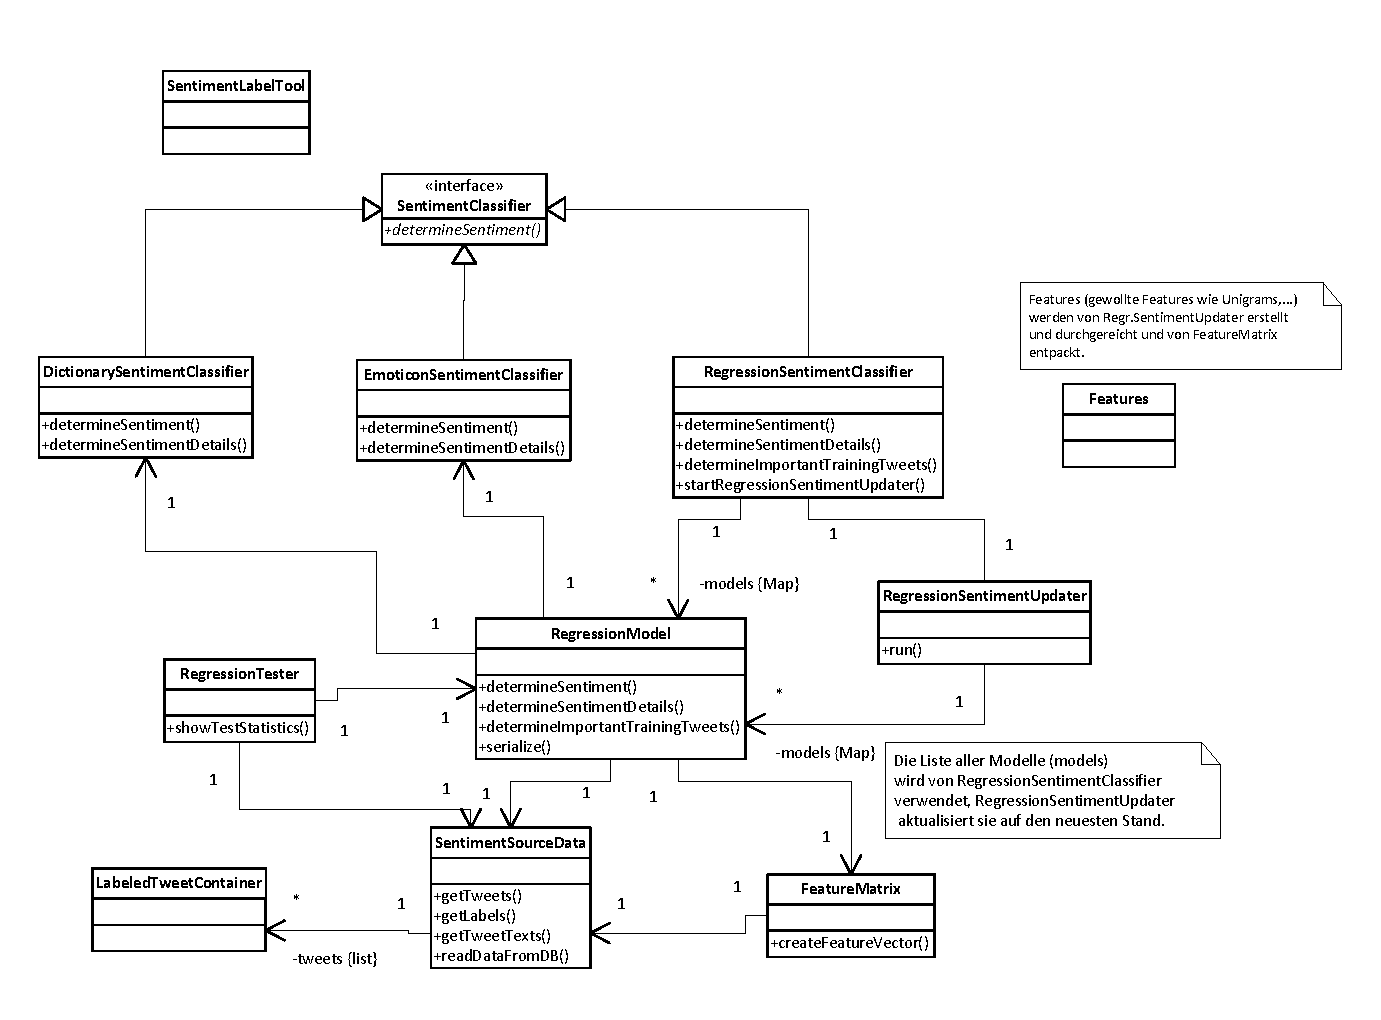
\includegraphics[width=\textwidth]{./Bilder/Sentiment/SentimentPackageClassDiagramm.pdf}
  \caption{Architektur des Pakets daemon.sentiment}
  \label{sentimentuml}
\end{figure}

Das Interface \texttt{Sentiment\-Classifier} definiert die Methode \texttt{determine\-Sentiment()}. Diese berechnet zu einem gegebenen Text in einer gegebenen Sprache den Sentimentwert. Drei Klassifikatoren implementieren dieses Interface, wobei jede der Implementierungen eine der vorgestellten Methoden umsetzt, Sentiment zu berechnen. Diese Klassen bilden die Schnittstelle des Sentiment-Pakets nach außen: Sie können von Daemon oder REST-Service instanziert werden (im Endprodukt wird der akkurateste Classifier, der \texttt{Regression\-Sentiment\-Classifier}, instanziert). Der Wörterbuch- und der Emoticon-Klassifikator erledigen alle anfallenden Aufgaben selbst. Der wichtigste Klassifikator, \texttt{Re\-gre\-ssion\-Sentiment\-Classifier}, greift zur Bewältigung seiner Aufgaben auf eine Reihe weiterer Klassen zurück, in deren Zentrum die Klasse \texttt{Regression\-Model} steht.

\subsubsection{Die Schnittstelle nach außen: Implementierungen von SentimentClassifier}
\label{sec:sentimentclassifier}

Der \texttt{Emoticon\-Sentiment\-Classifier} berechnet den Sentimentwert eines Textes auf Grundlage einer Emoticon-Liste, die in einem Abgleich mit dem Ergebnis der Twitter-Suche entstanden ist. Mit einer Twitter-Suche nach \textit{Merkel :-)} werden Tweets ausgegeben, die Twitter als positiv erkennt und die beispielsweise auch die Emoticons \textit{:-D} oder \textit{:-P} enthalten; analoges gilt für negative Tweets.

Der \texttt{Dictionary\-Sentiment\-Classifier} verwendet ein Wörterbuch, um den Sentimentwert eines Texts zu berechnen. Dabei kommen das ​Wörterbuch von Liu \cite{LiuLexicon}
 und die folgende Aggregierungsfunktion:

\[ \frac{\#pos - \#neg}{\#pos + \#neg} \]

Das Vorgehen ist damit dasselbe wie bei ​Stieglitz und Dang-Xuan (2012) \cite{Stieglitz2012}, allerdings mit einem anderen Wörterbuch, da das Wörterbuch von Liu im Gegensatz zum Wörterbuch des dort verwendeten Tools LIWC frei verfügbar ist. Beide beinhalten keine Gewichtungen für einzelne Wörter (z.\,B. ist "`super"' genauso positiv wie "`good"'), sodass die Aggregationsfunktion die Häufigkeit von positiven bzw. negativen Wörtern verwendet.

Das Wörterbuch wird "`roh"' verwendet, ohne grammatikalische Regeln, trotz der Warnung von Liu, dies nicht zu tun, sodass z.\,B. "`not happy"' positiv ist. Da aber vorgesehen ist, das Wörterbuch durch einen Machine-Learning-Algorithmus zu ersetzen, schien eine dahingehende Erweiterung der Wörterbuchklasse unsinnig.

Das Wörterbuch bewertet nur englischsprachige Tweets. Um zu erkennen, ob ein Tweet englischsprachig ist, wird der Rückgabewert der Twitter API-verwendet, die zu jedem Tweet einen zweistelligen ISO-Sprachcode liefert. Diese Klassifikation hat sich als ausreichend genau herausgestellt. Nicht-englischsprachige Tweets erhalten einen Sentimentwert von \texttt{null}. 

Die Klasse \texttt{Regression\-Sentiment\-Classifier} implementiert das Interface \texttt{Sentiment\-Classifier} und verwaltet die verschiedenen Regressionsmodelle. In einer Hashtabelle liegt für jede Sprache, für die genügend Trainings-Tweets vorliegen, ein Regressionsmodell. Als Schlüssel werden wiederum die zweistelligen ISO-Sprachcodes verwendet. Beim Start versucht der Classifier zunächst, bestehende, serialisierte Modelle von der Festplatte zu lesen und diese zu verwenden. Mit der Methode \texttt{start\-Regression\-Sentiment\-Updater()}, die vom Daemon aufgerufen wird, wird ein neuer Thread gestartet, der \texttt{Regression\-Sentiment\-Updater} (siehe \ref{sentimentupdater}), der sich darum kümmert, die Modelle neu zu trainieren, falls sie nicht auf der Festplatte lagen, und aktuell zu halten, wenn neue Trainingsdaten vorliegen. Schließlich stellt auch dieser Classifier die Methode \texttt{determine\-Sentiment()} zur Verfügung, die basierend auf der übergebenen Tweet-Sprache das richtige Modell auswählt (falls verfügbar) und den berechneten Sentimentwert des Tweets zurückgibt.

\subsubsection{Der Unterbau: RegressionModel und seine Helfer}
\label{sec:regressionmodel}

Die Klasse \texttt{Regression\-Sentiment\-Classifier} greift für die Berechnung auf weitere Klassen zurück, in deren Mittelpunkt das RegressionModel steht.

\texttt{Regression\-Model} kapselt ein Modell, das bei Instanzierung mit einem spezifischen Satz Trainingsdaten trainiert wird, d.\,h. die Merkmalsmatrix bestimmt und darauf basierend die Parameter schätzt. Für die anderen Klassen im Paket (insbesondere \texttt{Regression\-Tester}) stellt es Methoden zur Verfügung, die bestimmte Statistiken (z.\,B. die verwendeten Trainingsdaten, die geschätzten Parameter) ausgeben oder in TSV-Dateien exportieren, aber die einzigen \texttt{public}-Methoden sind auch hier \texttt{determine\-Sentiment()} und dessen Variationen, die das Sentiment eines neuen Textes auf Basis der Parameter bestimmen. Die Methode \texttt{train\-Model\-Gradient\-Descent()} implementiert den eigentlichen Algorithmus (siehe \ref{sentiment:gradientdescent}). Der Algorithmus wird mit Nullen als Parameterwerte initialisiert und so häufig wiederholt, bis sich die Schätzungen nur noch unwesentlich verändern.

\texttt{Feature\-Matrix} stellt die Matrix dar, die die extrahierten Features bzw. Einflussfaktoren enthält. Es kommen die folgenden Features zum Einsatz, welche am Beispielsatz "`I love puppies but I don't like kittens :-)"' veranschaulicht werden.

\begin{itemize}
\itemsep0em
\item \textbf{Anzahl positiver Emoticons}: Ein Rückgabewert aus \texttt{Emoticon\-Sentiment\-Classi\-fier}. Im Beispielsatz 1.
\item \textbf{Anzahl negativer Emoticons}: Ein Rückgabewert aus \texttt{Emoticon\-Sentiment\-Classi\-fier}. Im Beispielsatz 0.
\item \textbf{Emoticon-Sentiment}: Die Sentiment-Schätzung aus \texttt{Emoticon\-Sentiment\-Classi\-fier}. Im Beispielsatz 1.
\item \textbf{Anzahl positiver Wörter}: Ein Rückgabewert aus \texttt{Dictionary\-Sentiment\-Classi\-fier}. Im Beispielsatz 2.
\item \textbf{Anzahl negativer Wörter}: Ein Rückgabewert aus \texttt{Dictionary\-Sentiment\-Classi\-fier} Im Beispielsatz 0.
\item \textbf{Dictionary-Sentiment}: Die Sentiment-Schätzung aus \texttt{Dictionary\-Sentiment\-Clas\-si\-fier}. Im Beispielsatz 1.
\item \textbf{Unigrams}: Einzelne Wörter, z.\,B. "`I"', "`love"', ...
\item \textbf{Bigrams}: Zwei aufeinanderfolgende Wörter, z.\,B. "`I love"', "`love puppies"', ...
\item \textbf{Trigrams}: Drei aufeinanderfolgende Wörter, z.\,B. "`I love puppies"', "`love puppies but"', ...
\item \textbf{Fourgrams}: Vier aufeinanderfolgende Wörter, z.\,B. "`I love puppies but"', "`love puppies but I"', ...
\end{itemize}

Darüber hinaus gibt es zwei Optionen, die die bestehenden Features modifizieren, wenn sie angeschaltet sind:

\begin{itemize}
\itemsep0em
\item \textbf{Negation}: Jedem Wort, das als negiert erkannt wird, wird ein Suffix "`\$NEG\$"' angehängt. Aus dem Unigram "`like"' wird z.\,B. "`like \$NEG\$"'
\item \textbf{Part-of-Speech-Tagger}: Jedem Wort wird seine Wortart in Form eines \textit{part of speech tag} als Suffix angehängt. Aus dem Unigram "`like"' wird z.\,B. "`like \$VB\$"' (für \textit{verb})
\end{itemize}

\texttt{Sentiment\-Source\-Data} spiegelt die Regressionsdaten wieder, kapselt also eine Menge von Tweets. Dabei handelt es sich entweder um die Trainings- oder die Testdaten. Die Klasse stellt Methoden bereit, um diese Daten aus einer Datenbank zu laden. \texttt{Labeled\-Tweet\-Container} kapselt einen einzelnen Tweet und das dazugehörige, von Menschen bestimmte, echte Sentiment (\textit{Label}).

\texttt{Regression\-Tester} kapselt den Test eines bestimmten Modells mit einem bestimmten Satz Testdaten. In der produktiven Nutzung sollen natürlich alle verfügbaren Daten als Trainingsdaten verwendet werden, um eine möglichst gute Vorhersagekraft zu erreichen. Die Tester mit ihrer Main-Methode lassen sich aber in der Entwicklung und Analyse nutzen, um nur einen Teil der Daten als Trainingsdaten zu verwenden. Ebenso können mehrere Tester für dasselbe Modell erstellt werden, um die Vorhersagekraft des Modells an unterschiedlichen Testdatensätzen zu evaluieren, oder Tester für mehrere Modelle, um die Modelle zu vergleichen.

Außerdem wurden im Paket \texttt{tmetrics.util} Helfer implementiert:

\texttt{Sparse\-Matrix} ist eine Matrix. Einfach ein zweidimensionales Array zu nutzen, wäre bei Matrizen in dieser Größenordnung (schon bei 123 gelabelten Tweets gab es 814 Spalten) eine Speicherplatzverschwendung, weil sehr viele Nullen gespeichert werden. Daher werden hier nur die Positionen gespeichert, die ungleich 0 sind. Die Matrix ist als Liste von Listen von Tupeln realisiert. Jede innere Liste ist eine Zeile. Jedes Tupel ist (Spalte, Wert). Der Grund für diese Entscheidung ist, dass die Matrix typischerweise zeilenweise geschrieben und gelesen wird, Operationen, die so in \( \mathcal O(1) \) möglich sind. Zudem ist die Anzahl der Spalten von Interesse, weshalb diese in einer Membervariable vorgehalten und bei Änderungen aktualisiert wird. Die Klasse stellt außerdem Methoden für benötigte Operationen (z.\,B. die Multiplikation der transponierten Matrix mit einem Vektor) zur Verfügung.

\texttt{List\-Util} stellt Methoden zur Verfügung, die Berechnungen mit Listen von Floats ermöglichen, welche wir als Vektoren benutzen. Ein Beispiel ist die Skalarmultiplikation zweier Vektoren. \texttt{Linear\-Regression} stellt die eigentliche lineare Regression dar, die als Eingabe eine \texttt{Feature\-Matrix} und die Labels erwartet. Daraufhin wird eine Regression mittels Gradientenverfahren durchgeführt. Die geschätzten Parameter sowie Werte zur internen Beurteilung (z.\,B. die Fehler oder geschätzten Werte der Trainingsdaten) können anschließend abgefragt werden. 

\subsection{Einbindung in die Architektur}
\label{subsec:sentimenteinbindung}

Der Nutzer sieht Sentimentwerte im Front-End in verschiedenen Detailstufen, die in Abschnitt \ref{sec:showTweets} näher erläutert werden. In der Tweet-Ansicht werden die für einzelne Tweets ermittelten Sentimentwerte direkt aus der Datenbank geladen. Wenn sich der Nutzer die Ergebnisse der Sentiment-Berechnung in detaillierter Form ausgeben lässt, werden die Sentiment-Modelle dagegen von der Festplatte geladen. Wie die Ausgabe dieser detaillierten Informationen umgesetzt ist, zeigt Abbildung \ref{sentimentdetailarchitecture}.

\begin{figure}
 \centering
  \centering
    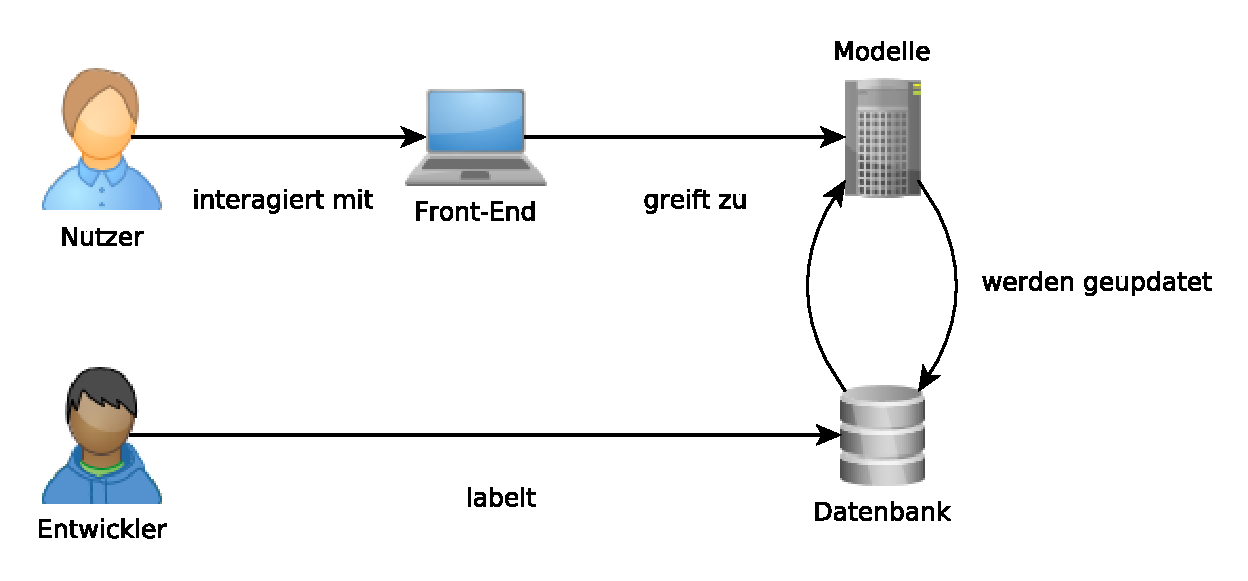
\includegraphics[width=\textwidth]{./Bilder/Sentiment/sentiment-architektur.pdf}
  \caption{Architektur aus Sicht des Sentiment-Pakets}
  \label{sentimentdetailarchitecture}
\end{figure}

Der Nutzer interagiert mit der Anwendung über das im Browser angezeigte Front-End. Seine Anfragen führen (via REST-Service) dazu, dass auf die Modelle zugegriffen wird, die auf der Festplatte liegen. Doch zeitgleich kann der Entwickler Tweets \texttt{labeln}, d.\,h., ihren Sentimentwert manuell bestimmen und so Trainingsdaten schaffen, um die Genauigkeit der Schätzungen zu verbessern. Deshalb müssen die Modelle aktuell gehalten werden, wenn neue Trainingsdaten vorliegen.

\texttt{Sentiment\-Label\-Tool} ist ein von der restlichen Anwendung unabhängiges Tool, das es ermöglicht, Tweets ohne direkten Zugriff auf die Datenbank und ohne Tools wie PHPMyAdmin zu labeln. Der Nutzer wählt die Sprache aus, in der Tweets gelabelt werden sollen. Dann wird ein Batch von 1000 Tweets geladen und der erste angezeigt. Der Nutzer gibt seine Bewertung in den Schritten -1, -0,5, 0, 0.5 oder 1 ein und bekommt anschließend den nächsten Tweet angezeigt. Tweets können auch übersprungen werden. Sobald zehn Tweets bearbeitet worden sind, wird der Batch vom Tool an die Datenbank gesendet und der nächste geholt. Der Grund für die unterschiedlichen Batch-Größen liegt darin, dass beim Laden 1000 zufällige Tweets ausgewählt werden. Diese Operation nimmt in MySQL einen sehr langen Zeitraum in Anspruch, dessen Dauer nicht von der Anzahl der abgefragten Tweets abhängt. Das Speichern von Sentimentwerten ist dagegen eine vergleichsweise schnelle Operation.

\label{sentimentupdater}

\texttt{Regression\-Sentiment\-Updater} läuft in einem eigenen Thread und kümmert sich um die Aktualisierung der Regressionsmodelle und die Sentiment-Aktualisierung aller Tweets in der Datenbank. Dazu überprüft er zunächst, ob neue Trainingsdaten zu einer beliebigen Sprache in der Datenbank vorhanden sind. Dies ist immer dann der Fall, wenn neue Tweets gelabelt worden sind. In diesem Fall wird eine Regression durchgeführt und das Modell gespeichert. Das Modell steht sofort als Java-Objekt dem \texttt{Regression\-Sentiment\-Classifier} zur Verfügung und wird für den Zugriff auch nach einem eventuellen Neustart des Daemons sowie für den REST-Service serialisiert und auf der Festplatte gespeichert. Anschließend wird das Sentiment aller Tweets in der Datenbank mit Hilfe des neuen Regressionsmodells berechnet und aktualisiert. Diese Überprüfung und die erneute Regression werden für alle Sprachen alle 24 Stunden durchgeführt. Das Programm ist somit selbst dafür zuständig, zu erkennen, ob es neue Modelle erstellen kann und es ist außer dem Labeln keine andere manuelle Intervention notwendig, um bessere Sentimentschätzungen zu erhalten.

\subsection{Diskussion}

Es lassen sich zwei Herausforderungen identifizieren, die sich bei der Umsetzung der Sentiment-Vorhersagen ergaben, nämlich die Überanpassung (\textit{overfitting}) und die Datenbankperformance. 

Voraussetzung für eine erfolgreiche Sentimentanalyse ist, dass die Sentimentwerte zu vielen Texten bereits bekannt sind. Die lineare Regression findet die optimalen Gewichte für die Vorhersage der Labels zu den Trainingsdaten. Dies bedeutet nicht notwendigerweise, dass neue Daten auch gut vorhergesagt werden. Der Begriff der Überanpassung an die Trainingsdaten beschreibt das Phänomen, dass Eigenheiten der Trainingsdaten, die nicht für andere Daten verallgemeinert werden können, vom Klassifikator zur Bewertung herangezogen werden. Überanpassung tritt auf, wenn die Zahl der Parameter bzw. Features zu hoch ist für die Anzahl der Datensätze.

Das heißt, dass die Überanpassung zu verringern ist, indem die Zahl der Datensätze erhöht oder die Zahl der Parameter gesenkt wird. Je mehr Trainingsdaten vorliegen, die zufällig aus dem Korpus ausgewählt sind, desto geringer wird der Einfluss einzelner Zufälle, aber Überanpassung kann nie ganz ausgeschlossen werden. Zum Beispiel könnte ein Begriff wie Irak auch über Jahre hinweg mit schlechten Nachrichten und erhitzten Debatten assoziiert sein. Mit diesen Daten trainiert, würde ein Klassifikator ihn (richtigerweise) zur Vorhersage negativer Emotion verwenden, und könnte vermutlich nicht verwendet werden, um Nachrichten über Irak aus einem anderen Themengebiet zu verwenden.

Die Überanpassung hat sich in diesem Projekt wie folgt geäußert: Zur Einschätzung des Sentimentwertes eines neuen Tweets können offensichtlich nur Features verwendet werden, die dem Modell bereits aus den Trainingsdaten bekannt sind. Obwohl mehr als 1000 manuell annotierte Tweets (deutsche und englische) als Trainingsdaten verwendet wurden, kam es regelmäßig vor, dass in den Testdaten Wörter vorkamen, die zweifellos zur emotionalen Aussage des Tweets beitrugen, aber nicht in den Trainingsdaten vorhanden gewesen waren und somit nicht zur Schätzung des Sentiments verwendet werden konnten. Das Feature wurde nicht erkannt, der entsprechende Parameterwert fehlt im Modell. Da bei einer linearen Regression mit n-Gramm-Features der Sentimentwert des Texts die Summe der Parameter der einzelnen n-Gramme ist, führt dieses Fehlen von Parameterwerten zu einer (absolut) zu niedrigen Schätzung.

Hinzu kommt, dass für den Algorithmus bei einem Mangel an Trainingsdaten nicht ersichtlich ist, welche Features für die Einschätzung des Sentimentwerts wichtig sind und welche nicht. Implizit werden häufige Features stärker gewichtet, denn wenn in einer Iteration des Gradientenabstiegsverfahrens der Parameterwert eines häufigen Features besser wird, hat dies einen höheren Einfluss auf den Fehler des Modells als bei einem seltenen Feature. Dieser Unterschied ist allerdings nur dann ausgeprägt, wenn ausreichend Trainingsdaten vorliegen. Wenn er nicht ausgeprägt ist, wie in unserem Fall, erhalten auch seltene Features, beispielsweise Fourgrams, vergleichsweise hohe Parameterwerte, und häufige Features vergleichsweise niedrige. Wird dieses Modell auf neue Daten angewandt, und werden dabei nur einige der vorliegenden Features erkannt, kommt es hierdurch wiederum verstärkt zu einer (absolut) zu niedrigen Schätzung. Es liegt ein Bias zugunsten absolut niedriger Sentimentwerte vor.

Zur Behebung des Problems wurden unterschiedliche Lösungsansätze versucht. Der vielversprechendste war, die Features auf all jene zu begrenzen, die mindestens in zwei Trainingsdatensätzen vorkamen. So nahmen wir zwar in Kauf, dass noch weniger Features wiedererkannt würden, erhofften uns aber auch, dass bei den tatsächlich wiedererkannten Features die Parameterwerte absolut höher sein würden. Dennoch ließ sich der Bias so nicht beseitigen.
Schließlich beschlossen wir, das Problem zu umgehen: Vorrangiges Ziel war die Einordnung der Tweets in negative, neutrale und positive. Diese Einordnung funktioniert trotz des Bias gut, wenn die Grenzen zwischen den Kategorien ebenfalls auf absolut niedrige Werte gesetzt werden.

Im Ergebnis empfehlen wir für den praktischen Einsatz die weitere Erhöhung der Zahl der Trainingstweets und möglicherweise die Verringerung der Anzahl Features mithilfe von Algorithmen zur \textit{feature selection}. Um den beschriebenen Bias zu verhindern, erscheinen nichtlineare Algorithmen vielversprechend, die besser mit dem Fehlen von Features umgehen können.

Neben der Überanpassung war die Datenbank-Performance eine Schwierigkeit. Gerade der \texttt{Regression\-Sentiment\-Updater} hat die komplexe Aufgabe, die Sentimentwerte aller Tweets in der Datenbank zu ändern, wenn neue Daten gelabelt worden sind. Im produktiven Einsatz kommt dies zwar kaum vor, während der Entwicklung dagegen umso häufiger. Bei mehreren Millionen Tweets nehmen die nötigen Datenbankoperationen eine große Menge Zeit und Ressourcen in Anspruch. Diese Aufgabe ist erfolgreich gelöst worden. Als hilfreich hat sich insbesondere das Profiling erwiesen, also das Aufzeichnen von Methodenlaufzeiten und verwendetem Speicher, um Bottlenecks zu identifizieren. Eine aktzeptable Laufzeit und ein geringer Speicherverbrauch wurden schließlich durch die Verwendung geeigneter \textit{batched statements} in Verbindung mit manuellen Commits sowie einem \textit{streaming result set}.
%\section{Cluster-Analyse}
\section{Cluster-Analyse}
%Wladimir
In der frühen Phase des Projektseminars wurden verschiedene Ideen für das 
Projekt vorgeschlagen. Eine der Ideen beschäftigte sich mit dem Gedanken, 
die Tweets als Punkte zu repräsentieren und damit explorativ zu arbeiten.
Dabei sollte es möglich sein, durch die Entfernung zwi\-schen den Tweets zu
sehen, ob zwei Tweets zu einem Thema gehören und eher die selbe Meinung vertreten oder nicht. Die Abbildung 
\ref{fig:ClusteringIdee} illustriert die vorgestellte Idee, wobei die einzelnen Symbole 
die Tweets repräsentieren und zu Clustern zusammengefasst sind. Damit kann ein Benutzer sehen, welche Gruppen sich bilden und wie die Meinungen zu einem bestimmten Thema aussehen. Es könnte dabei um die Entscheidung gehen,
welchen Film man sich angucken möchte, aber auch um die Entwicklung eines 
neuen Produktes, wobei das neue Produkt möglichst die Wünsche der Benutzer erfüllen sollte.
Dies motivierte die Implementierung einer Cluster-Analyse für Tweets.

\begin{figure}[h]
 \centering
 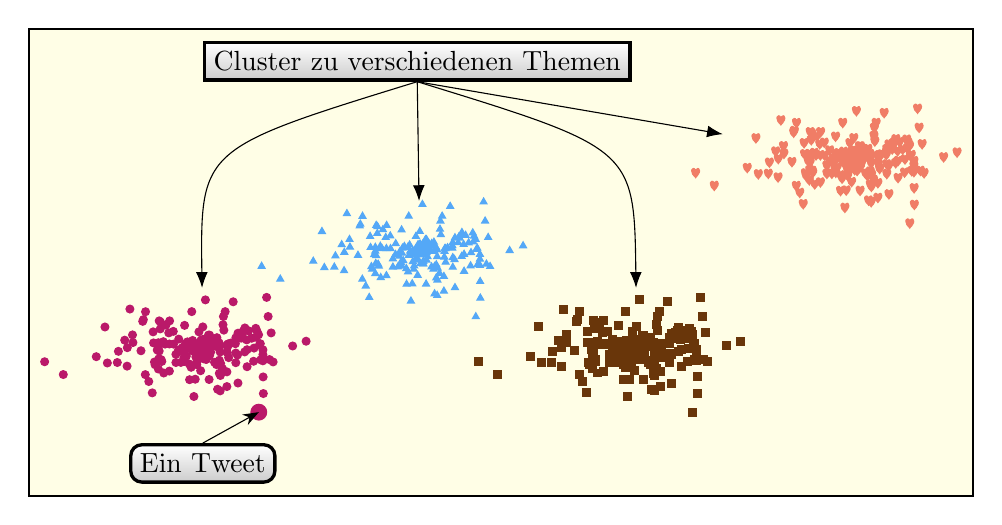
\begin{tikzpicture}[y=\textwidth/100,x=\textwidth/44, background rectangle/.style={draw=black, thick, fill=yellow!10,},show background rectangle]
\def\marRad{0.5mm}
\definecolor{color0}{rgb}{0.73,0.10,0.41}
\definecolor{color1}{rgb}{0.41,0.21,0.04}
\definecolor{color2}{rgb}{0.33,0.66,0.97}
\definecolor{color3}{rgb}{0.71,0.00,0.15}
\definecolor{color4}{rgb}{0.96,0.16,0.94}
\definecolor{color5}{rgb}{0.55,0.95,0.91}
\definecolor{color6}{rgb}{0.94,0.49,0.40}

\path[fill=color0,draw=color0,mark size=\marRad, mark=*] plot coordinates {(11.03, 13.77)};
\path[fill=color0,draw=color0,mark size=\marRad, mark=*] plot coordinates {(10.76, 8.68)};
\path[fill=color0,draw=color0,mark size=\marRad, mark=*] plot coordinates {(10.76, 7.31)};
\path[fill=color0,draw=color0,mark size=\marRad, mark=*] plot coordinates {(14.14, 10.17)};
\path[fill=color0,draw=color0,mark size=\marRad, mark=*] plot coordinates {(10.55, 10.86)};
\path[fill=color0,draw=color0,mark size=\marRad, mark=*] plot coordinates {(10.40, 10.60)};
\path[fill=color0,draw=color0,mark size=\marRad, mark=*] plot coordinates {(10.28, 10.79)};
\path[fill=color0,draw=color0,mark size=\marRad, mark=*] plot coordinates {(9.16, 12.33)};
\path[fill=color0,draw=color0,mark size=\marRad, mark=*] plot coordinates {(10.02, 10.47)};
\path[fill=color0,draw=color0,mark size=\marRad, mark=*] plot coordinates {(10.01, 10.02)};
\path[fill=color0,draw=color0,mark size=\marRad, mark=*] plot coordinates {(12.57, 11.35)};
\path[fill=color0,draw=color0,mark size=\marRad, mark=*] plot coordinates {(11.40, 14.80)};
\path[fill=color0,draw=color0,mark size=\marRad, mark=*] plot coordinates {(11.14, 10.08)};
\path[fill=color0,draw=color0,mark size=\marRad, mark=*] plot coordinates {(8.46, 7.54)};
\path[fill=color0,draw=color0,mark size=\marRad, mark=*] plot coordinates {(6.78, 10.53)};
\path[fill=color0,draw=color0,mark size=\marRad, mark=*] plot coordinates {(10.01, 10.41)};
\path[fill=color0,draw=color0,mark size=\marRad, mark=*] plot coordinates {(11.13, 9.48)};
\path[fill=color0,draw=color0,mark size=\marRad, mark=*] plot coordinates {(9.65, 6.69)};
\path[fill=color0,draw=color0,mark size=\marRad, mark=*] plot coordinates {(11.88, 11.76)};
\path[fill=color0,draw=color0,mark size=\marRad, mark=*] plot coordinates {(7.51, 6.45)};
\path[fill=color0,draw=color0,mark size=\marRad, mark=*] plot coordinates {(12.79, 5.19)};
\path[fill=color0,draw=color0,mark size=\marRad, mark=*] plot coordinates {(11.52, 9.43)};
\path[fill=color0,draw=color0,mark size=\marRad, mark=*] plot coordinates {(10.00, 10.00)};
\path[fill=color0,draw=color0,mark size=\marRad, mark=*] plot coordinates {(10.19, 9.88)};
\path[fill=color0,draw=color0,mark size=\marRad, mark=*] plot coordinates {(5.49, 12.16)};
\path[fill=color0,draw=color0,mark size=2*\marRad, mark=*] plot coordinates {(12.58, 3.24)};
\path[fill=color0,draw=color0,mark size=\marRad, mark=*] plot coordinates {(11.15, 10.37)};
\path[fill=color0,draw=color0,mark size=\marRad, mark=*] plot coordinates {(11.28, 10.47)};
\path[fill=color0,draw=color0,mark size=\marRad, mark=*] plot coordinates {(9.68, 9.02)};
\path[fill=color0,draw=color0,mark size=\marRad, mark=*] plot coordinates {(10.95, 13.26)};
\path[fill=color0,draw=color0,mark size=\marRad, mark=*] plot coordinates {(9.72, 8.21)};
\path[fill=color0,draw=color0,mark size=\marRad, mark=*] plot coordinates {(12.04, 9.78)};
\path[fill=color0,draw=color0,mark size=\marRad, mark=*] plot coordinates {(10.55, 10.90)};
\path[fill=color0,draw=color0,mark size=\marRad, mark=*] plot coordinates {(9.24, 9.11)};
\path[fill=color0,draw=color0,mark size=\marRad, mark=*] plot coordinates {(10.17, 10.60)};
\path[fill=color0,draw=color0,mark size=\marRad, mark=*] plot coordinates {(9.86, 9.20)};
\path[fill=color0,draw=color0,mark size=\marRad, mark=*] plot coordinates {(10.01, 10.01)};
\path[fill=color0,draw=color0,mark size=\marRad, mark=*] plot coordinates {(9.80, 9.22)};
\path[fill=color0,draw=color0,mark size=\marRad, mark=*] plot coordinates {(9.80, 9.82)};
\path[fill=color0,draw=color0,mark size=\marRad, mark=*] plot coordinates {(10.31, 9.96)};
\path[fill=color0,draw=color0,mark size=\marRad, mark=*] plot coordinates {(7.99, 9.64)};
\path[fill=color0,draw=color0,mark size=\marRad, mark=*] plot coordinates {(9.50, 9.67)};
\path[fill=color0,draw=color0,mark size=\marRad, mark=*] plot coordinates {(8.11, 8.55)};
\path[fill=color0,draw=color0,mark size=\marRad, mark=*] plot coordinates {(8.30, 12.36)};
\path[fill=color0,draw=color0,mark size=\marRad, mark=*] plot coordinates {(11.11, 5.92)};
\path[fill=color0,draw=color0,mark size=\marRad, mark=*] plot coordinates {(12.04, 8.00)};
\path[fill=color0,draw=color0,mark size=\marRad, mark=*] plot coordinates {(7.23, 12.75)};
\path[fill=color0,draw=color0,mark size=\marRad, mark=*] plot coordinates {(10.16, 8.78)};
\path[fill=color0,draw=color0,mark size=\marRad, mark=*] plot coordinates {(10.80, 10.23)};
\path[fill=color0,draw=color0,mark size=\marRad, mark=*] plot coordinates {(8.65, 10.37)};
\path[fill=color0,draw=color0,mark size=\marRad, mark=*] plot coordinates {(11.50, 10.68)};
\path[fill=color0,draw=color0,mark size=\marRad, mark=*] plot coordinates {(9.83, 9.72)};
\path[fill=color0,draw=color0,mark size=\marRad, mark=*] plot coordinates {(10.01, 10.86)};
\path[fill=color0,draw=color0,mark size=\marRad, mark=*] plot coordinates {(10.14, 10.52)};
\path[fill=color0,draw=color0,mark size=\marRad, mark=*] plot coordinates {(11.62, 6.29)};
\path[fill=color0,draw=color0,mark size=\marRad, mark=*] plot coordinates {(12.65, 10.41)};
\path[fill=color0,draw=color0,mark size=\marRad, mark=*] plot coordinates {(11.93, 9.55)};
\path[fill=color0,draw=color0,mark size=\marRad, mark=*] plot coordinates {(7.67, 5.26)};
\path[fill=color0,draw=color0,mark size=\marRad, mark=*] plot coordinates {(9.90, 7.58)};
\path[fill=color0,draw=color0,mark size=\marRad, mark=*] plot coordinates {(12.67, 8.72)};
\path[fill=color0,draw=color0,mark size=\marRad, mark=*] plot coordinates {(12.11, 11.76)};
\path[fill=color0,draw=color0,mark size=\marRad, mark=*] plot coordinates {(10.68, 5.64)};
\path[fill=color0,draw=color0,mark size=\marRad, mark=*] plot coordinates {(10.61, 10.66)};
\path[fill=color0,draw=color0,mark size=\marRad, mark=*] plot coordinates {(11.60, 9.23)};
\path[fill=color0,draw=color0,mark size=\marRad, mark=*] plot coordinates {(8.99, 8.45)};
\path[fill=color0,draw=color0,mark size=\marRad, mark=*] plot coordinates {(11.50, 10.41)};
\path[fill=color0,draw=color0,mark size=\marRad, mark=*] plot coordinates {(10.31, 11.31)};
\path[fill=color0,draw=color0,mark size=\marRad, mark=*] plot coordinates {(12.44, 12.02)};
\path[fill=color0,draw=color0,mark size=\marRad, mark=*] plot coordinates {(12.77, 8.62)};
\path[fill=color0,draw=color0,mark size=\marRad, mark=*] plot coordinates {(7.71, 11.65)};
\path[fill=color0,draw=color0,mark size=\marRad, mark=*] plot coordinates {(10.29, 6.66)};
\path[fill=color0,draw=color0,mark size=\marRad, mark=*] plot coordinates {(10.82, 8.34)};
\path[fill=color0,draw=color0,mark size=\marRad, mark=*] plot coordinates {(13.01, 13.26)};
\path[fill=color0,draw=color0,mark size=\marRad, mark=*] plot coordinates {(2.71, 8.52)};
\path[fill=color0,draw=color0,mark size=\marRad, mark=*] plot coordinates {(10.26, 11.31)};
\path[fill=color0,draw=color0,mark size=\marRad, mark=*] plot coordinates {(10.80, 5.47)};
\path[fill=color0,draw=color0,mark size=\marRad, mark=*] plot coordinates {(8.26, 10.37)};
\path[fill=color0,draw=color0,mark size=\marRad, mark=*] plot coordinates {(12.36, 9.95)};
\path[fill=color0,draw=color0,mark size=\marRad, mark=*] plot coordinates {(7.35, 7.17)};
\path[fill=color0,draw=color0,mark size=\marRad, mark=*] plot coordinates {(9.92, 9.19)};
\path[fill=color0,draw=color0,mark size=\marRad, mark=*] plot coordinates {(5.60, 8.39)};
\path[fill=color0,draw=color0,mark size=\marRad, mark=*] plot coordinates {(10.00, 12.17)};
\path[fill=color0,draw=color0,mark size=\marRad, mark=*] plot coordinates {(10.16, 9.04)};
\path[fill=color0,draw=color0,mark size=\marRad, mark=*] plot coordinates {(10.03, 10.52)};
\path[fill=color0,draw=color0,mark size=\marRad, mark=*] plot coordinates {(8.47, 12.80)};
\path[fill=color0,draw=color0,mark size=\marRad, mark=*] plot coordinates {(10.44, 10.32)};
\path[fill=color0,draw=color0,mark size=\marRad, mark=*] plot coordinates {(12.25, 10.98)};
\path[fill=color0,draw=color0,mark size=\marRad, mark=*] plot coordinates {(6.76, 11.33)};
\path[fill=color0,draw=color0,mark size=\marRad, mark=*] plot coordinates {(10.63, 8.22)};
\path[fill=color0,draw=color0,mark size=\marRad, mark=*] plot coordinates {(11.52, 8.42)};
\path[fill=color0,draw=color0,mark size=\marRad, mark=*] plot coordinates {(9.29, 10.60)};
\path[fill=color0,draw=color0,mark size=\marRad, mark=*] plot coordinates {(9.92, 10.79)};
\path[fill=color0,draw=color0,mark size=\marRad, mark=*] plot coordinates {(9.70, 9.85)};
\path[fill=color0,draw=color0,mark size=\marRad, mark=*] plot coordinates {(9.91, 9.92)};
\path[fill=color0,draw=color0,mark size=\marRad, mark=*] plot coordinates {(11.80, 11.60)};
\path[fill=color0,draw=color0,mark size=\marRad, mark=*] plot coordinates {(10.93, 12.40)};
\path[fill=color0,draw=color0,mark size=\marRad, mark=*] plot coordinates {(9.17, 8.55)};
\path[fill=color0,draw=color0,mark size=\marRad, mark=*] plot coordinates {(12.50, 11.69)};
\path[fill=color0,draw=color0,mark size=\marRad, mark=*] plot coordinates {(7.99, 12.80)};
\path[fill=color0,draw=color0,mark size=\marRad, mark=*] plot coordinates {(10.16, 10.05)};
\path[fill=color0,draw=color0,mark size=\marRad, mark=*] plot coordinates {(7.97, 8.82)};
\path[fill=color0,draw=color0,mark size=\marRad, mark=*] plot coordinates {(7.26, 12.93)};
\path[fill=color0,draw=color0,mark size=\marRad, mark=*] plot coordinates {(10.13, 10.84)};
\path[fill=color0,draw=color0,mark size=\marRad, mark=*] plot coordinates {(9.67, 10.12)};
\path[fill=color0,draw=color0,mark size=\marRad, mark=*] plot coordinates {(11.11, 7.46)};
\path[fill=color0,draw=color0,mark size=\marRad, mark=*] plot coordinates {(8.20, 7.34)};
\path[fill=color0,draw=color0,mark size=\marRad, mark=*] plot coordinates {(11.18, 10.38)};
\path[fill=color0,draw=color0,mark size=\marRad, mark=*] plot coordinates {(14.76, 10.67)};
\path[fill=color0,draw=color0,mark size=\marRad, mark=*] plot coordinates {(7.77, 8.49)};
\path[fill=color0,draw=color0,mark size=\marRad, mark=*] plot coordinates {(12.77, 9.27)};
\path[fill=color0,draw=color0,mark size=\marRad, mark=*] plot coordinates {(9.69, 10.06)};
\path[fill=color0,draw=color0,mark size=\marRad, mark=*] plot coordinates {(8.05, 12.68)};
\path[fill=color0,draw=color0,mark size=\marRad, mark=*] plot coordinates {(10.11, 9.76)};
\path[fill=color0,draw=color0,mark size=\marRad, mark=*] plot coordinates {(10.00, 10.35)};
\path[fill=color0,draw=color0,mark size=\marRad, mark=*] plot coordinates {(9.93, 10.65)};
\path[fill=color0,draw=color0,mark size=\marRad, mark=*] plot coordinates {(9.46, 7.94)};
\path[fill=color0,draw=color0,mark size=\marRad, mark=*] plot coordinates {(13.07, 8.75)};
\path[fill=color0,draw=color0,mark size=\marRad, mark=*] plot coordinates {(11.52, 11.02)};
\path[fill=color0,draw=color0,mark size=\marRad, mark=*] plot coordinates {(10.04, 8.83)};
\path[fill=color0,draw=color0,mark size=\marRad, mark=*] plot coordinates {(9.13, 8.94)};
\path[fill=color0,draw=color0,mark size=\marRad, mark=*] plot coordinates {(8.46, 10.38)};
\path[fill=color0,draw=color0,mark size=\marRad, mark=*] plot coordinates {(11.62, 11.51)};
\path[fill=color0,draw=color0,mark size=\marRad, mark=*] plot coordinates {(10.17, 10.06)};
\path[fill=color0,draw=color0,mark size=\marRad, mark=*] plot coordinates {(6.06, 8.44)};
\path[fill=color0,draw=color0,mark size=\marRad, mark=*] plot coordinates {(9.45, 10.51)};
\path[fill=color0,draw=color0,mark size=\marRad, mark=*] plot coordinates {(12.02, 10.81)};
\path[fill=color0,draw=color0,mark size=\marRad, mark=*] plot coordinates {(10.81, 7.08)};
\path[fill=color0,draw=color0,mark size=\marRad, mark=*] plot coordinates {(11.19, 8.95)};
\path[fill=color0,draw=color0,mark size=\marRad, mark=*] plot coordinates {(10.41, 10.92)};
\path[fill=color0,draw=color0,mark size=\marRad, mark=*] plot coordinates {(7.36, 13.76)};
\path[fill=color0,draw=color0,mark size=\marRad, mark=*] plot coordinates {(7.73, 10.49)};
\path[fill=color0,draw=color0,mark size=\marRad, mark=*] plot coordinates {(10.54, 8.46)};
\path[fill=color0,draw=color0,mark size=\marRad, mark=*] plot coordinates {(7.95, 10.51)};
\path[fill=color0,draw=color0,mark size=\marRad, mark=*] plot coordinates {(9.99, 9.90)};
\path[fill=color0,draw=color0,mark size=\marRad, mark=*] plot coordinates {(3.57, 7.18)};
\path[fill=color0,draw=color0,mark size=\marRad, mark=*] plot coordinates {(7.80, 8.21)};
\path[fill=color0,draw=color0,mark size=\marRad, mark=*] plot coordinates {(11.94, 12.06)};
\path[fill=color0,draw=color0,mark size=\marRad, mark=*] plot coordinates {(8.89, 10.89)};
\path[fill=color0,draw=color0,mark size=\marRad, mark=*] plot coordinates {(10.23, 10.42)};
\path[fill=color0,draw=color0,mark size=\marRad, mark=*] plot coordinates {(12.61, 10.29)};
\path[fill=color0,draw=color0,mark size=\marRad, mark=*] plot coordinates {(9.80, 10.18)};
\path[fill=color0,draw=color0,mark size=\marRad, mark=*] plot coordinates {(10.97, 11.83)};
\path[fill=color0,draw=color0,mark size=\marRad, mark=*] plot coordinates {(8.04, 11.96)};
\path[fill=color0,draw=color0,mark size=\marRad, mark=*] plot coordinates {(10.14, 9.91)};
\path[fill=color0,draw=color0,mark size=\marRad, mark=*] plot coordinates {(10.65, 11.04)};
\path[fill=color0,draw=color0,mark size=\marRad, mark=*] plot coordinates {(10.12, 15.00)};
\path[fill=color0,draw=color0,mark size=\marRad, mark=*] plot coordinates {(11.77, 10.99)};
\path[fill=color0,draw=color0,mark size=\marRad, mark=*] plot coordinates {(9.49, 13.77)};
\path[fill=color0,draw=color0,mark size=\marRad, mark=*] plot coordinates {(12.78, 6.93)};
\path[fill=color0,draw=color0,mark size=\marRad, mark=*] plot coordinates {(7.95, 7.76)};
\path[fill=color0,draw=color0,mark size=\marRad, mark=*] plot coordinates {(8.76, 8.44)};
\path[fill=color0,draw=color0,mark size=\marRad, mark=*] plot coordinates {(10.74, 10.34)};
\path[fill=color0,draw=color0,mark size=\marRad, mark=*] plot coordinates {(5.09, 9.05)};
\path[fill=color0,draw=color0,mark size=\marRad, mark=*] plot coordinates {(12.34, 8.57)};
\path[fill=color0,draw=color0,mark size=\marRad, mark=*] plot coordinates {(9.20, 10.42)};
\path[fill=color0,draw=color0,mark size=\marRad, mark=*] plot coordinates {(9.07, 10.02)};
\path[fill=color0,draw=color0,mark size=\marRad, mark=*] plot coordinates {(8.76, 9.30)};
\path[fill=color0,draw=color0,mark size=\marRad, mark=*] plot coordinates {(8.18, 10.62)};
\path[fill=color0,draw=color0,mark size=\marRad, mark=*] plot coordinates {(12.94, 15.26)};
\path[fill=color0,draw=color0,mark size=\marRad, mark=*] plot coordinates {(10.91, 7.79)};
\path[fill=color0,draw=color0,mark size=\marRad, mark=*] plot coordinates {(9.74, 8.57)};
\path[fill=color0,draw=color0,mark size=\marRad, mark=*] plot coordinates {(9.18, 9.89)};
\path[fill=color0,draw=color0,mark size=\marRad, mark=*] plot coordinates {(8.88, 9.76)};
\path[fill=color0,draw=color0,mark size=\marRad, mark=*] plot coordinates {(9.82, 11.65)};
\path[fill=color0,draw=color0,mark size=\marRad, mark=*] plot coordinates {(12.46, 11.08)};
\path[fill=color0,draw=color0,mark size=\marRad, mark=*] plot coordinates {(7.90, 9.75)};
\path[fill=color0,draw=color0,mark size=\marRad, mark=*] plot coordinates {(9.39, 6.64)};
\path[fill=color0,draw=color0,mark size=\marRad, mark=*] plot coordinates {(9.68, 9.94)};
\path[fill=color0,draw=color0,mark size=\marRad, mark=*] plot coordinates {(8.64, 11.70)};
\path[fill=color0,draw=color0,mark size=\marRad, mark=*] plot coordinates {(13.24, 8.50)};
\path[fill=color0,draw=color0,mark size=\marRad, mark=*] plot coordinates {(6.40, 10.78)};
\path[fill=color0,draw=color0,mark size=\marRad, mark=*] plot coordinates {(10.68, 8.50)};
\path[fill=color0,draw=color0,mark size=\marRad, mark=*] plot coordinates {(10.01, 10.02)};
\path[fill=color0,draw=color0,mark size=\marRad, mark=*] plot coordinates {(10.15, 8.76)};
\path[fill=color0,draw=color0,mark size=\marRad, mark=*] plot coordinates {(8.43, 11.54)};
\path[fill=color0,draw=color0,mark size=\marRad, mark=*] plot coordinates {(9.93, 10.43)};
\path[fill=color0,draw=color0,mark size=\marRad, mark=*] plot coordinates {(10.01, 10.00)};
\path[fill=color0,draw=color0,mark size=\marRad, mark=*] plot coordinates {(9.59, 4.88)};
\path[fill=color0,draw=color0,mark size=\marRad, mark=*] plot coordinates {(10.31, 9.16)};
\path[fill=color0,draw=color0,mark size=\marRad, mark=*] plot coordinates {(11.83, 11.48)};
\path[fill=color0,draw=color0,mark size=\marRad, mark=*] plot coordinates {(6.51, 8.06)};
\path[fill=color0,draw=color0,mark size=\marRad, mark=*] plot coordinates {(10.41, 10.10)};
\path[fill=color0,draw=color0,mark size=\marRad, mark=*] plot coordinates {(10.75, 10.50)};
\path[fill=color0,draw=color0,mark size=\marRad, mark=*] plot coordinates {(9.05, 9.59)};
\path[fill=color0,draw=color0,mark size=\marRad, mark=*] plot coordinates {(6.64, 14.04)};
\path[fill=color0,draw=color0,mark size=\marRad, mark=*] plot coordinates {(10.66, 10.08)};
\path[fill=color0,draw=color0,mark size=\marRad, mark=*] plot coordinates {(9.38, 8.28)};
\path[fill=color0,draw=color0,mark size=\marRad, mark=*] plot coordinates {(8.08, 8.74)};
\path[fill=color0,draw=color0,mark size=\marRad, mark=*] plot coordinates {(12.77, 9.77)};
\path[fill=color0,draw=color0,mark size=\marRad, mark=*] plot coordinates {(10.80, 9.54)};
\path[fill=color0,draw=color0,mark size=\marRad, mark=*] plot coordinates {(9.82, 10.37)};
\path[fill=color0,draw=color0,mark size=\marRad, mark=*] plot coordinates {(6.11, 9.61)};
\path[fill=color0,draw=color0,mark size=\marRad, mark=*] plot coordinates {(7.15, 9.67)};
\path[fill=color0,draw=color0,mark size=\marRad, mark=*] plot coordinates {(9.56, 10.12)};
\path[fill=color0,draw=color0,mark size=\marRad, mark=*] plot coordinates {(7.95, 10.11)};
\path[fill=color0,draw=color0,mark size=\marRad, mark=*] plot coordinates {(10.36, 9.52)};
\path[fill=color0,draw=color0,mark size=\marRad, mark=*] plot coordinates {(13.15, 11.54)};
\path[fill=color0,draw=color0,mark size=\marRad, mark=*] plot coordinates {(10.06, 9.72)};
\path[fill=color0,draw=color0,mark size=\marRad, mark=*] plot coordinates {(9.53, 10.75)};
\path[fill=color0,draw=color0,mark size=\marRad, mark=*] plot coordinates {(6.52, 9.99)};
\path[fill=color1,draw=color1,mark size=\marRad, mark=square*] plot coordinates {(31.03, 13.77)};
\path[fill=color1,draw=color1,mark size=\marRad, mark=square*] plot coordinates {(30.76, 8.68)};
\path[fill=color1,draw=color1,mark size=\marRad, mark=square*] plot coordinates {(30.76, 7.31)};
\path[fill=color1,draw=color1,mark size=\marRad, mark=square*] plot coordinates {(34.14, 10.17)};
\path[fill=color1,draw=color1,mark size=\marRad, mark=square*] plot coordinates {(30.55, 10.86)};
\path[fill=color1,draw=color1,mark size=\marRad, mark=square*] plot coordinates {(30.40, 10.60)};
\path[fill=color1,draw=color1,mark size=\marRad, mark=square*] plot coordinates {(30.28, 10.79)};
\path[fill=color1,draw=color1,mark size=\marRad, mark=square*] plot coordinates {(29.16, 12.33)};
\path[fill=color1,draw=color1,mark size=\marRad, mark=square*] plot coordinates {(30.02, 10.47)};
\path[fill=color1,draw=color1,mark size=\marRad, mark=square*] plot coordinates {(30.01, 10.02)};
\path[fill=color1,draw=color1,mark size=\marRad, mark=square*] plot coordinates {(32.57, 11.35)};
\path[fill=color1,draw=color1,mark size=\marRad, mark=square*] plot coordinates {(31.40, 14.80)};
\path[fill=color1,draw=color1,mark size=\marRad, mark=square*] plot coordinates {(31.14, 10.08)};
\path[fill=color1,draw=color1,mark size=\marRad, mark=square*] plot coordinates {(28.46, 7.54)};
\path[fill=color1,draw=color1,mark size=\marRad, mark=square*] plot coordinates {(26.78, 10.53)};
\path[fill=color1,draw=color1,mark size=\marRad, mark=square*] plot coordinates {(30.01, 10.41)};
\path[fill=color1,draw=color1,mark size=\marRad, mark=square*] plot coordinates {(31.13, 9.48)};
\path[fill=color1,draw=color1,mark size=\marRad, mark=square*] plot coordinates {(29.65, 6.69)};
\path[fill=color1,draw=color1,mark size=\marRad, mark=square*] plot coordinates {(31.88, 11.76)};
\path[fill=color1,draw=color1,mark size=\marRad, mark=square*] plot coordinates {(27.51, 6.45)};
\path[fill=color1,draw=color1,mark size=\marRad, mark=square*] plot coordinates {(32.79, 5.19)};
\path[fill=color1,draw=color1,mark size=\marRad, mark=square*] plot coordinates {(31.52, 9.43)};
\path[fill=color1,draw=color1,mark size=\marRad, mark=square*] plot coordinates {(30.00, 10.00)};
\path[fill=color1,draw=color1,mark size=\marRad, mark=square*] plot coordinates {(30.19, 9.88)};
\path[fill=color1,draw=color1,mark size=\marRad, mark=square*] plot coordinates {(25.49, 12.16)};
\path[fill=color1,draw=color1,mark size=\marRad, mark=square*] plot coordinates {(32.58, 3.24)};
\path[fill=color1,draw=color1,mark size=\marRad, mark=square*] plot coordinates {(31.15, 10.37)};
\path[fill=color1,draw=color1,mark size=\marRad, mark=square*] plot coordinates {(31.28, 10.47)};
\path[fill=color1,draw=color1,mark size=\marRad, mark=square*] plot coordinates {(29.68, 9.02)};
\path[fill=color1,draw=color1,mark size=\marRad, mark=square*] plot coordinates {(30.95, 13.26)};
\path[fill=color1,draw=color1,mark size=\marRad, mark=square*] plot coordinates {(29.72, 8.21)};
\path[fill=color1,draw=color1,mark size=\marRad, mark=square*] plot coordinates {(32.04, 9.78)};
\path[fill=color1,draw=color1,mark size=\marRad, mark=square*] plot coordinates {(30.55, 10.90)};
\path[fill=color1,draw=color1,mark size=\marRad, mark=square*] plot coordinates {(29.24, 9.11)};
\path[fill=color1,draw=color1,mark size=\marRad, mark=square*] plot coordinates {(30.17, 10.60)};
\path[fill=color1,draw=color1,mark size=\marRad, mark=square*] plot coordinates {(29.86, 9.20)};
\path[fill=color1,draw=color1,mark size=\marRad, mark=square*] plot coordinates {(30.01, 10.01)};
\path[fill=color1,draw=color1,mark size=\marRad, mark=square*] plot coordinates {(29.80, 9.22)};
\path[fill=color1,draw=color1,mark size=\marRad, mark=square*] plot coordinates {(29.80, 9.82)};
\path[fill=color1,draw=color1,mark size=\marRad, mark=square*] plot coordinates {(30.31, 9.96)};
\path[fill=color1,draw=color1,mark size=\marRad, mark=square*] plot coordinates {(27.99, 9.64)};
\path[fill=color1,draw=color1,mark size=\marRad, mark=square*] plot coordinates {(29.50, 9.67)};
\path[fill=color1,draw=color1,mark size=\marRad, mark=square*] plot coordinates {(28.11, 8.55)};
\path[fill=color1,draw=color1,mark size=\marRad, mark=square*] plot coordinates {(28.30, 12.36)};
\path[fill=color1,draw=color1,mark size=\marRad, mark=square*] plot coordinates {(31.11, 5.92)};
\path[fill=color1,draw=color1,mark size=\marRad, mark=square*] plot coordinates {(32.04, 8.00)};
\path[fill=color1,draw=color1,mark size=\marRad, mark=square*] plot coordinates {(27.23, 12.75)};
\path[fill=color1,draw=color1,mark size=\marRad, mark=square*] plot coordinates {(30.16, 8.78)};
\path[fill=color1,draw=color1,mark size=\marRad, mark=square*] plot coordinates {(30.80, 10.23)};
\path[fill=color1,draw=color1,mark size=\marRad, mark=square*] plot coordinates {(28.65, 10.37)};
\path[fill=color1,draw=color1,mark size=\marRad, mark=square*] plot coordinates {(31.50, 10.68)};
\path[fill=color1,draw=color1,mark size=\marRad, mark=square*] plot coordinates {(29.83, 9.72)};
\path[fill=color1,draw=color1,mark size=\marRad, mark=square*] plot coordinates {(30.01, 10.86)};
\path[fill=color1,draw=color1,mark size=\marRad, mark=square*] plot coordinates {(30.14, 10.52)};
\path[fill=color1,draw=color1,mark size=\marRad, mark=square*] plot coordinates {(31.62, 6.29)};
\path[fill=color1,draw=color1,mark size=\marRad, mark=square*] plot coordinates {(32.65, 10.41)};
\path[fill=color1,draw=color1,mark size=\marRad, mark=square*] plot coordinates {(31.93, 9.55)};
\path[fill=color1,draw=color1,mark size=\marRad, mark=square*] plot coordinates {(27.67, 5.26)};
\path[fill=color1,draw=color1,mark size=\marRad, mark=square*] plot coordinates {(29.90, 7.58)};
\path[fill=color1,draw=color1,mark size=\marRad, mark=square*] plot coordinates {(32.67, 8.72)};
\path[fill=color1,draw=color1,mark size=\marRad, mark=square*] plot coordinates {(32.11, 11.76)};
\path[fill=color1,draw=color1,mark size=\marRad, mark=square*] plot coordinates {(30.68, 5.64)};
\path[fill=color1,draw=color1,mark size=\marRad, mark=square*] plot coordinates {(30.61, 10.66)};
\path[fill=color1,draw=color1,mark size=\marRad, mark=square*] plot coordinates {(31.60, 9.23)};
\path[fill=color1,draw=color1,mark size=\marRad, mark=square*] plot coordinates {(28.99, 8.45)};
\path[fill=color1,draw=color1,mark size=\marRad, mark=square*] plot coordinates {(31.50, 10.41)};
\path[fill=color1,draw=color1,mark size=\marRad, mark=square*] plot coordinates {(30.31, 11.31)};
\path[fill=color1,draw=color1,mark size=\marRad, mark=square*] plot coordinates {(32.44, 12.02)};
\path[fill=color1,draw=color1,mark size=\marRad, mark=square*] plot coordinates {(32.77, 8.62)};
\path[fill=color1,draw=color1,mark size=\marRad, mark=square*] plot coordinates {(27.71, 11.65)};
\path[fill=color1,draw=color1,mark size=\marRad, mark=square*] plot coordinates {(30.29, 6.66)};
\path[fill=color1,draw=color1,mark size=\marRad, mark=square*] plot coordinates {(30.82, 8.34)};
\path[fill=color1,draw=color1,mark size=\marRad, mark=square*] plot coordinates {(33.01, 13.26)};
\path[fill=color1,draw=color1,mark size=\marRad, mark=square*] plot coordinates {(22.71, 8.52)};
\path[fill=color1,draw=color1,mark size=\marRad, mark=square*] plot coordinates {(30.26, 11.31)};
\path[fill=color1,draw=color1,mark size=\marRad, mark=square*] plot coordinates {(30.80, 5.47)};
\path[fill=color1,draw=color1,mark size=\marRad, mark=square*] plot coordinates {(28.26, 10.37)};
\path[fill=color1,draw=color1,mark size=\marRad, mark=square*] plot coordinates {(32.36, 9.95)};
\path[fill=color1,draw=color1,mark size=\marRad, mark=square*] plot coordinates {(27.35, 7.17)};
\path[fill=color1,draw=color1,mark size=\marRad, mark=square*] plot coordinates {(29.92, 9.19)};
\path[fill=color1,draw=color1,mark size=\marRad, mark=square*] plot coordinates {(25.60, 8.39)};
\path[fill=color1,draw=color1,mark size=\marRad, mark=square*] plot coordinates {(30.00, 12.17)};
\path[fill=color1,draw=color1,mark size=\marRad, mark=square*] plot coordinates {(30.16, 9.04)};
\path[fill=color1,draw=color1,mark size=\marRad, mark=square*] plot coordinates {(30.03, 10.52)};
\path[fill=color1,draw=color1,mark size=\marRad, mark=square*] plot coordinates {(28.47, 12.80)};
\path[fill=color1,draw=color1,mark size=\marRad, mark=square*] plot coordinates {(30.44, 10.32)};
\path[fill=color1,draw=color1,mark size=\marRad, mark=square*] plot coordinates {(32.25, 10.98)};
\path[fill=color1,draw=color1,mark size=\marRad, mark=square*] plot coordinates {(26.76, 11.33)};
\path[fill=color1,draw=color1,mark size=\marRad, mark=square*] plot coordinates {(30.63, 8.22)};
\path[fill=color1,draw=color1,mark size=\marRad, mark=square*] plot coordinates {(31.52, 8.42)};
\path[fill=color1,draw=color1,mark size=\marRad, mark=square*] plot coordinates {(29.29, 10.60)};
\path[fill=color1,draw=color1,mark size=\marRad, mark=square*] plot coordinates {(29.92, 10.79)};
\path[fill=color1,draw=color1,mark size=\marRad, mark=square*] plot coordinates {(29.70, 9.85)};
\path[fill=color1,draw=color1,mark size=\marRad, mark=square*] plot coordinates {(29.91, 9.92)};
\path[fill=color1,draw=color1,mark size=\marRad, mark=square*] plot coordinates {(31.80, 11.60)};
\path[fill=color1,draw=color1,mark size=\marRad, mark=square*] plot coordinates {(30.93, 12.40)};
\path[fill=color1,draw=color1,mark size=\marRad, mark=square*] plot coordinates {(29.17, 8.55)};
\path[fill=color1,draw=color1,mark size=\marRad, mark=square*] plot coordinates {(32.50, 11.69)};
\path[fill=color1,draw=color1,mark size=\marRad, mark=square*] plot coordinates {(27.99, 12.80)};
\path[fill=color1,draw=color1,mark size=\marRad, mark=square*] plot coordinates {(30.16, 10.05)};
\path[fill=color1,draw=color1,mark size=\marRad, mark=square*] plot coordinates {(27.97, 8.82)};
\path[fill=color1,draw=color1,mark size=\marRad, mark=square*] plot coordinates {(27.26, 12.93)};
\path[fill=color1,draw=color1,mark size=\marRad, mark=square*] plot coordinates {(30.13, 10.84)};
\path[fill=color1,draw=color1,mark size=\marRad, mark=square*] plot coordinates {(29.67, 10.12)};
\path[fill=color1,draw=color1,mark size=\marRad, mark=square*] plot coordinates {(31.11, 7.46)};
\path[fill=color1,draw=color1,mark size=\marRad, mark=square*] plot coordinates {(28.20, 7.34)};
\path[fill=color1,draw=color1,mark size=\marRad, mark=square*] plot coordinates {(31.18, 10.38)};
\path[fill=color1,draw=color1,mark size=\marRad, mark=square*] plot coordinates {(34.76, 10.67)};
\path[fill=color1,draw=color1,mark size=\marRad, mark=square*] plot coordinates {(27.77, 8.49)};
\path[fill=color1,draw=color1,mark size=\marRad, mark=square*] plot coordinates {(32.77, 9.27)};
\path[fill=color1,draw=color1,mark size=\marRad, mark=square*] plot coordinates {(29.69, 10.06)};
\path[fill=color1,draw=color1,mark size=\marRad, mark=square*] plot coordinates {(28.05, 12.68)};
\path[fill=color1,draw=color1,mark size=\marRad, mark=square*] plot coordinates {(30.11, 9.76)};
\path[fill=color1,draw=color1,mark size=\marRad, mark=square*] plot coordinates {(30.00, 10.35)};
\path[fill=color1,draw=color1,mark size=\marRad, mark=square*] plot coordinates {(29.93, 10.65)};
\path[fill=color1,draw=color1,mark size=\marRad, mark=square*] plot coordinates {(29.46, 7.94)};
\path[fill=color1,draw=color1,mark size=\marRad, mark=square*] plot coordinates {(33.07, 8.75)};
\path[fill=color1,draw=color1,mark size=\marRad, mark=square*] plot coordinates {(31.52, 11.02)};
\path[fill=color1,draw=color1,mark size=\marRad, mark=square*] plot coordinates {(30.04, 8.83)};
\path[fill=color1,draw=color1,mark size=\marRad, mark=square*] plot coordinates {(29.13, 8.94)};
\path[fill=color1,draw=color1,mark size=\marRad, mark=square*] plot coordinates {(28.46, 10.38)};
\path[fill=color1,draw=color1,mark size=\marRad, mark=square*] plot coordinates {(31.62, 11.51)};
\path[fill=color1,draw=color1,mark size=\marRad, mark=square*] plot coordinates {(30.17, 10.06)};
\path[fill=color1,draw=color1,mark size=\marRad, mark=square*] plot coordinates {(26.06, 8.44)};
\path[fill=color1,draw=color1,mark size=\marRad, mark=square*] plot coordinates {(29.45, 10.51)};
\path[fill=color1,draw=color1,mark size=\marRad, mark=square*] plot coordinates {(32.02, 10.81)};
\path[fill=color1,draw=color1,mark size=\marRad, mark=square*] plot coordinates {(30.81, 7.08)};
\path[fill=color1,draw=color1,mark size=\marRad, mark=square*] plot coordinates {(31.19, 8.95)};
\path[fill=color1,draw=color1,mark size=\marRad, mark=square*] plot coordinates {(30.41, 10.92)};
\path[fill=color1,draw=color1,mark size=\marRad, mark=square*] plot coordinates {(27.36, 13.76)};
\path[fill=color1,draw=color1,mark size=\marRad, mark=square*] plot coordinates {(27.73, 10.49)};
\path[fill=color1,draw=color1,mark size=\marRad, mark=square*] plot coordinates {(30.54, 8.46)};
\path[fill=color1,draw=color1,mark size=\marRad, mark=square*] plot coordinates {(27.95, 10.51)};
\path[fill=color1,draw=color1,mark size=\marRad, mark=square*] plot coordinates {(29.99, 9.90)};
\path[fill=color1,draw=color1,mark size=\marRad, mark=square*] plot coordinates {(23.57, 7.18)};
\path[fill=color1,draw=color1,mark size=\marRad, mark=square*] plot coordinates {(27.80, 8.21)};
\path[fill=color1,draw=color1,mark size=\marRad, mark=square*] plot coordinates {(31.94, 12.06)};
\path[fill=color1,draw=color1,mark size=\marRad, mark=square*] plot coordinates {(28.89, 10.89)};
\path[fill=color1,draw=color1,mark size=\marRad, mark=square*] plot coordinates {(30.23, 10.42)};
\path[fill=color1,draw=color1,mark size=\marRad, mark=square*] plot coordinates {(32.61, 10.29)};
\path[fill=color1,draw=color1,mark size=\marRad, mark=square*] plot coordinates {(29.80, 10.18)};
\path[fill=color1,draw=color1,mark size=\marRad, mark=square*] plot coordinates {(30.97, 11.83)};
\path[fill=color1,draw=color1,mark size=\marRad, mark=square*] plot coordinates {(28.04, 11.96)};
\path[fill=color1,draw=color1,mark size=\marRad, mark=square*] plot coordinates {(30.14, 9.91)};
\path[fill=color1,draw=color1,mark size=\marRad, mark=square*] plot coordinates {(30.65, 11.04)};
\path[fill=color1,draw=color1,mark size=\marRad, mark=square*] plot coordinates {(30.12, 15.00)};
\path[fill=color1,draw=color1,mark size=\marRad, mark=square*] plot coordinates {(31.77, 10.99)};
\path[fill=color1,draw=color1,mark size=\marRad, mark=square*] plot coordinates {(29.49, 13.77)};
\path[fill=color1,draw=color1,mark size=\marRad, mark=square*] plot coordinates {(32.78, 6.93)};
\path[fill=color1,draw=color1,mark size=\marRad, mark=square*] plot coordinates {(27.95, 7.76)};
\path[fill=color1,draw=color1,mark size=\marRad, mark=square*] plot coordinates {(28.76, 8.44)};
\path[fill=color1,draw=color1,mark size=\marRad, mark=square*] plot coordinates {(30.74, 10.34)};
\path[fill=color1,draw=color1,mark size=\marRad, mark=square*] plot coordinates {(25.09, 9.05)};
\path[fill=color1,draw=color1,mark size=\marRad, mark=square*] plot coordinates {(32.34, 8.57)};
\path[fill=color1,draw=color1,mark size=\marRad, mark=square*] plot coordinates {(29.20, 10.42)};
\path[fill=color1,draw=color1,mark size=\marRad, mark=square*] plot coordinates {(29.07, 10.02)};
\path[fill=color1,draw=color1,mark size=\marRad, mark=square*] plot coordinates {(28.76, 9.30)};
\path[fill=color1,draw=color1,mark size=\marRad, mark=square*] plot coordinates {(28.18, 10.62)};
\path[fill=color1,draw=color1,mark size=\marRad, mark=square*] plot coordinates {(32.94, 15.26)};
\path[fill=color1,draw=color1,mark size=\marRad, mark=square*] plot coordinates {(30.91, 7.79)};
\path[fill=color1,draw=color1,mark size=\marRad, mark=square*] plot coordinates {(29.74, 8.57)};
\path[fill=color1,draw=color1,mark size=\marRad, mark=square*] plot coordinates {(29.18, 9.89)};
\path[fill=color1,draw=color1,mark size=\marRad, mark=square*] plot coordinates {(28.88, 9.76)};
\path[fill=color1,draw=color1,mark size=\marRad, mark=square*] plot coordinates {(29.82, 11.65)};
\path[fill=color1,draw=color1,mark size=\marRad, mark=square*] plot coordinates {(32.46, 11.08)};
\path[fill=color1,draw=color1,mark size=\marRad, mark=square*] plot coordinates {(27.90, 9.75)};
\path[fill=color1,draw=color1,mark size=\marRad, mark=square*] plot coordinates {(29.39, 6.64)};
\path[fill=color1,draw=color1,mark size=\marRad, mark=square*] plot coordinates {(29.68, 9.94)};
\path[fill=color1,draw=color1,mark size=\marRad, mark=square*] plot coordinates {(28.64, 11.70)};
\path[fill=color1,draw=color1,mark size=\marRad, mark=square*] plot coordinates {(33.24, 8.50)};
\path[fill=color1,draw=color1,mark size=\marRad, mark=square*] plot coordinates {(26.40, 10.78)};
\path[fill=color1,draw=color1,mark size=\marRad, mark=square*] plot coordinates {(30.68, 8.50)};
\path[fill=color1,draw=color1,mark size=\marRad, mark=square*] plot coordinates {(30.01, 10.02)};
\path[fill=color1,draw=color1,mark size=\marRad, mark=square*] plot coordinates {(30.15, 8.76)};
\path[fill=color1,draw=color1,mark size=\marRad, mark=square*] plot coordinates {(28.43, 11.54)};
\path[fill=color1,draw=color1,mark size=\marRad, mark=square*] plot coordinates {(29.93, 10.43)};
\path[fill=color1,draw=color1,mark size=\marRad, mark=square*] plot coordinates {(30.01, 10.00)};
\path[fill=color1,draw=color1,mark size=\marRad, mark=square*] plot coordinates {(29.59, 4.88)};
\path[fill=color1,draw=color1,mark size=\marRad, mark=square*] plot coordinates {(30.31, 9.16)};
\path[fill=color1,draw=color1,mark size=\marRad, mark=square*] plot coordinates {(31.83, 11.48)};
\path[fill=color1,draw=color1,mark size=\marRad, mark=square*] plot coordinates {(26.51, 8.06)};
\path[fill=color1,draw=color1,mark size=\marRad, mark=square*] plot coordinates {(30.41, 10.10)};
\path[fill=color1,draw=color1,mark size=\marRad, mark=square*] plot coordinates {(30.75, 10.50)};
\path[fill=color1,draw=color1,mark size=\marRad, mark=square*] plot coordinates {(29.05, 9.59)};
\path[fill=color1,draw=color1,mark size=\marRad, mark=square*] plot coordinates {(26.64, 14.04)};
\path[fill=color1,draw=color1,mark size=\marRad, mark=square*] plot coordinates {(30.66, 10.08)};
\path[fill=color1,draw=color1,mark size=\marRad, mark=square*] plot coordinates {(29.38, 8.28)};
\path[fill=color1,draw=color1,mark size=\marRad, mark=square*] plot coordinates {(28.08, 8.74)};
\path[fill=color1,draw=color1,mark size=\marRad, mark=square*] plot coordinates {(32.77, 9.77)};
\path[fill=color1,draw=color1,mark size=\marRad, mark=square*] plot coordinates {(30.80, 9.54)};
\path[fill=color1,draw=color1,mark size=\marRad, mark=square*] plot coordinates {(29.82, 10.37)};
\path[fill=color1,draw=color1,mark size=\marRad, mark=square*] plot coordinates {(26.11, 9.61)};
\path[fill=color1,draw=color1,mark size=\marRad, mark=square*] plot coordinates {(27.15, 9.67)};
\path[fill=color1,draw=color1,mark size=\marRad, mark=square*] plot coordinates {(29.56, 10.12)};
\path[fill=color1,draw=color1,mark size=\marRad, mark=square*] plot coordinates {(27.95, 10.11)};
\path[fill=color1,draw=color1,mark size=\marRad, mark=square*] plot coordinates {(30.36, 9.52)};
\path[fill=color1,draw=color1,mark size=\marRad, mark=square*] plot coordinates {(33.15, 11.54)};
\path[fill=color1,draw=color1,mark size=\marRad, mark=square*] plot coordinates {(30.06, 9.72)};
\path[fill=color1,draw=color1,mark size=\marRad, mark=square*] plot coordinates {(29.53, 10.75)};
\path[fill=color1,draw=color1,mark size=\marRad, mark=square*] plot coordinates {(26.52, 9.99)};
\path[fill=color2,draw=color2,mark size=\marRad, mark=triangle*] plot coordinates {(21.03, 23.77)};
\path[fill=color2,draw=color2,mark size=\marRad, mark=triangle*] plot coordinates {(20.76, 18.68)};
\path[fill=color2,draw=color2,mark size=\marRad, mark=triangle*] plot coordinates {(20.76, 17.31)};
\path[fill=color2,draw=color2,mark size=\marRad, mark=triangle*] plot coordinates {(24.14, 20.17)};
\path[fill=color2,draw=color2,mark size=\marRad, mark=triangle*] plot coordinates {(20.55, 20.86)};
\path[fill=color2,draw=color2,mark size=\marRad, mark=triangle*] plot coordinates {(20.40, 20.60)};
\path[fill=color2,draw=color2,mark size=\marRad, mark=triangle*] plot coordinates {(20.28, 20.79)};
\path[fill=color2,draw=color2,mark size=\marRad, mark=triangle*] plot coordinates {(19.16, 22.33)};
\path[fill=color2,draw=color2,mark size=\marRad, mark=triangle*] plot coordinates {(20.02, 20.47)};
\path[fill=color2,draw=color2,mark size=\marRad, mark=triangle*] plot coordinates {(20.01, 20.02)};
\path[fill=color2,draw=color2,mark size=\marRad, mark=triangle*] plot coordinates {(22.57, 21.35)};
\path[fill=color2,draw=color2,mark size=\marRad, mark=triangle*] plot coordinates {(21.40, 24.80)};
\path[fill=color2,draw=color2,mark size=\marRad, mark=triangle*] plot coordinates {(21.14, 20.08)};
\path[fill=color2,draw=color2,mark size=\marRad, mark=triangle*] plot coordinates {(18.46, 17.54)};
\path[fill=color2,draw=color2,mark size=\marRad, mark=triangle*] plot coordinates {(16.78, 20.53)};
\path[fill=color2,draw=color2,mark size=\marRad, mark=triangle*] plot coordinates {(20.01, 20.41)};
\path[fill=color2,draw=color2,mark size=\marRad, mark=triangle*] plot coordinates {(21.13, 19.48)};
\path[fill=color2,draw=color2,mark size=\marRad, mark=triangle*] plot coordinates {(19.65, 16.69)};
\path[fill=color2,draw=color2,mark size=\marRad, mark=triangle*] plot coordinates {(21.88, 21.76)};
\path[fill=color2,draw=color2,mark size=\marRad, mark=triangle*] plot coordinates {(17.51, 16.45)};
\path[fill=color2,draw=color2,mark size=\marRad, mark=triangle*] plot coordinates {(22.79, 15.19)};
\path[fill=color2,draw=color2,mark size=\marRad, mark=triangle*] plot coordinates {(21.52, 19.43)};
\path[fill=color2,draw=color2,mark size=\marRad, mark=triangle*] plot coordinates {(20.00, 20.00)};
\path[fill=color2,draw=color2,mark size=\marRad, mark=triangle*] plot coordinates {(20.19, 19.88)};
\path[fill=color2,draw=color2,mark size=\marRad, mark=triangle*] plot coordinates {(15.49, 22.16)};
\path[fill=color2,draw=color2,mark size=\marRad, mark=triangle*] plot coordinates {(22.58, 13.24)};
\path[fill=color2,draw=color2,mark size=\marRad, mark=triangle*] plot coordinates {(21.15, 20.37)};
\path[fill=color2,draw=color2,mark size=\marRad, mark=triangle*] plot coordinates {(21.28, 20.47)};
\path[fill=color2,draw=color2,mark size=\marRad, mark=triangle*] plot coordinates {(19.68, 19.02)};
\path[fill=color2,draw=color2,mark size=\marRad, mark=triangle*] plot coordinates {(20.95, 23.26)};
\path[fill=color2,draw=color2,mark size=\marRad, mark=triangle*] plot coordinates {(19.72, 18.21)};
\path[fill=color2,draw=color2,mark size=\marRad, mark=triangle*] plot coordinates {(22.04, 19.78)};
\path[fill=color2,draw=color2,mark size=\marRad, mark=triangle*] plot coordinates {(20.55, 20.90)};
\path[fill=color2,draw=color2,mark size=\marRad, mark=triangle*] plot coordinates {(19.24, 19.11)};
\path[fill=color2,draw=color2,mark size=\marRad, mark=triangle*] plot coordinates {(20.17, 20.60)};
\path[fill=color2,draw=color2,mark size=\marRad, mark=triangle*] plot coordinates {(19.86, 19.20)};
\path[fill=color2,draw=color2,mark size=\marRad, mark=triangle*] plot coordinates {(20.01, 20.01)};
\path[fill=color2,draw=color2,mark size=\marRad, mark=triangle*] plot coordinates {(19.80, 19.22)};
\path[fill=color2,draw=color2,mark size=\marRad, mark=triangle*] plot coordinates {(19.80, 19.82)};
\path[fill=color2,draw=color2,mark size=\marRad, mark=triangle*] plot coordinates {(20.31, 19.96)};
\path[fill=color2,draw=color2,mark size=\marRad, mark=triangle*] plot coordinates {(17.99, 19.64)};
\path[fill=color2,draw=color2,mark size=\marRad, mark=triangle*] plot coordinates {(19.50, 19.67)};
\path[fill=color2,draw=color2,mark size=\marRad, mark=triangle*] plot coordinates {(18.11, 18.55)};
\path[fill=color2,draw=color2,mark size=\marRad, mark=triangle*] plot coordinates {(18.30, 22.36)};
\path[fill=color2,draw=color2,mark size=\marRad, mark=triangle*] plot coordinates {(21.11, 15.92)};
\path[fill=color2,draw=color2,mark size=\marRad, mark=triangle*] plot coordinates {(22.04, 18.00)};
\path[fill=color2,draw=color2,mark size=\marRad, mark=triangle*] plot coordinates {(17.23, 22.75)};
\path[fill=color2,draw=color2,mark size=\marRad, mark=triangle*] plot coordinates {(20.16, 18.78)};
\path[fill=color2,draw=color2,mark size=\marRad, mark=triangle*] plot coordinates {(20.80, 20.23)};
\path[fill=color2,draw=color2,mark size=\marRad, mark=triangle*] plot coordinates {(18.65, 20.37)};
\path[fill=color2,draw=color2,mark size=\marRad, mark=triangle*] plot coordinates {(21.50, 20.68)};
\path[fill=color2,draw=color2,mark size=\marRad, mark=triangle*] plot coordinates {(19.83, 19.72)};
\path[fill=color2,draw=color2,mark size=\marRad, mark=triangle*] plot coordinates {(20.01, 20.86)};
\path[fill=color2,draw=color2,mark size=\marRad, mark=triangle*] plot coordinates {(20.14, 20.52)};
\path[fill=color2,draw=color2,mark size=\marRad, mark=triangle*] plot coordinates {(21.62, 16.29)};
\path[fill=color2,draw=color2,mark size=\marRad, mark=triangle*] plot coordinates {(22.65, 20.41)};
\path[fill=color2,draw=color2,mark size=\marRad, mark=triangle*] plot coordinates {(21.93, 19.55)};
\path[fill=color2,draw=color2,mark size=\marRad, mark=triangle*] plot coordinates {(17.67, 15.26)};
\path[fill=color2,draw=color2,mark size=\marRad, mark=triangle*] plot coordinates {(19.90, 17.58)};
\path[fill=color2,draw=color2,mark size=\marRad, mark=triangle*] plot coordinates {(22.67, 18.72)};
\path[fill=color2,draw=color2,mark size=\marRad, mark=triangle*] plot coordinates {(22.11, 21.76)};
\path[fill=color2,draw=color2,mark size=\marRad, mark=triangle*] plot coordinates {(20.68, 15.64)};
\path[fill=color2,draw=color2,mark size=\marRad, mark=triangle*] plot coordinates {(20.61, 20.66)};
\path[fill=color2,draw=color2,mark size=\marRad, mark=triangle*] plot coordinates {(21.60, 19.23)};
\path[fill=color2,draw=color2,mark size=\marRad, mark=triangle*] plot coordinates {(18.99, 18.45)};
\path[fill=color2,draw=color2,mark size=\marRad, mark=triangle*] plot coordinates {(21.50, 20.41)};
\path[fill=color2,draw=color2,mark size=\marRad, mark=triangle*] plot coordinates {(20.31, 21.31)};
\path[fill=color2,draw=color2,mark size=\marRad, mark=triangle*] plot coordinates {(22.44, 22.02)};
\path[fill=color2,draw=color2,mark size=\marRad, mark=triangle*] plot coordinates {(22.77, 18.62)};
\path[fill=color2,draw=color2,mark size=\marRad, mark=triangle*] plot coordinates {(17.71, 21.65)};
\path[fill=color2,draw=color2,mark size=\marRad, mark=triangle*] plot coordinates {(20.29, 16.66)};
\path[fill=color2,draw=color2,mark size=\marRad, mark=triangle*] plot coordinates {(20.82, 18.34)};
\path[fill=color2,draw=color2,mark size=\marRad, mark=triangle*] plot coordinates {(23.01, 23.26)};
\path[fill=color2,draw=color2,mark size=\marRad, mark=triangle*] plot coordinates {(12.71, 18.52)};
\path[fill=color2,draw=color2,mark size=\marRad, mark=triangle*] plot coordinates {(20.26, 21.31)};
\path[fill=color2,draw=color2,mark size=\marRad, mark=triangle*] plot coordinates {(20.80, 15.47)};
\path[fill=color2,draw=color2,mark size=\marRad, mark=triangle*] plot coordinates {(18.26, 20.37)};
\path[fill=color2,draw=color2,mark size=\marRad, mark=triangle*] plot coordinates {(22.36, 19.95)};
\path[fill=color2,draw=color2,mark size=\marRad, mark=triangle*] plot coordinates {(17.35, 17.17)};
\path[fill=color2,draw=color2,mark size=\marRad, mark=triangle*] plot coordinates {(19.92, 19.19)};
\path[fill=color2,draw=color2,mark size=\marRad, mark=triangle*] plot coordinates {(15.60, 18.39)};
\path[fill=color2,draw=color2,mark size=\marRad, mark=triangle*] plot coordinates {(20.00, 22.17)};
\path[fill=color2,draw=color2,mark size=\marRad, mark=triangle*] plot coordinates {(20.16, 19.04)};
\path[fill=color2,draw=color2,mark size=\marRad, mark=triangle*] plot coordinates {(20.03, 20.52)};
\path[fill=color2,draw=color2,mark size=\marRad, mark=triangle*] plot coordinates {(18.47, 22.80)};
\path[fill=color2,draw=color2,mark size=\marRad, mark=triangle*] plot coordinates {(20.44, 20.32)};
\path[fill=color2,draw=color2,mark size=\marRad, mark=triangle*] plot coordinates {(22.25, 20.98)};
\path[fill=color2,draw=color2,mark size=\marRad, mark=triangle*] plot coordinates {(16.76, 21.33)};
\path[fill=color2,draw=color2,mark size=\marRad, mark=triangle*] plot coordinates {(20.63, 18.22)};
\path[fill=color2,draw=color2,mark size=\marRad, mark=triangle*] plot coordinates {(21.52, 18.42)};
\path[fill=color2,draw=color2,mark size=\marRad, mark=triangle*] plot coordinates {(19.29, 20.60)};
\path[fill=color2,draw=color2,mark size=\marRad, mark=triangle*] plot coordinates {(19.92, 20.79)};
\path[fill=color2,draw=color2,mark size=\marRad, mark=triangle*] plot coordinates {(19.70, 19.85)};
\path[fill=color2,draw=color2,mark size=\marRad, mark=triangle*] plot coordinates {(19.91, 19.92)};
\path[fill=color2,draw=color2,mark size=\marRad, mark=triangle*] plot coordinates {(21.80, 21.60)};
\path[fill=color2,draw=color2,mark size=\marRad, mark=triangle*] plot coordinates {(20.93, 22.40)};
\path[fill=color2,draw=color2,mark size=\marRad, mark=triangle*] plot coordinates {(19.17, 18.55)};
\path[fill=color2,draw=color2,mark size=\marRad, mark=triangle*] plot coordinates {(22.50, 21.69)};
\path[fill=color2,draw=color2,mark size=\marRad, mark=triangle*] plot coordinates {(17.99, 22.80)};
\path[fill=color2,draw=color2,mark size=\marRad, mark=triangle*] plot coordinates {(20.16, 20.05)};
\path[fill=color2,draw=color2,mark size=\marRad, mark=triangle*] plot coordinates {(17.97, 18.82)};
\path[fill=color2,draw=color2,mark size=\marRad, mark=triangle*] plot coordinates {(17.26, 22.93)};
\path[fill=color2,draw=color2,mark size=\marRad, mark=triangle*] plot coordinates {(20.13, 20.84)};
\path[fill=color2,draw=color2,mark size=\marRad, mark=triangle*] plot coordinates {(19.67, 20.12)};
\path[fill=color2,draw=color2,mark size=\marRad, mark=triangle*] plot coordinates {(21.11, 17.46)};
\path[fill=color2,draw=color2,mark size=\marRad, mark=triangle*] plot coordinates {(18.20, 17.34)};
\path[fill=color2,draw=color2,mark size=\marRad, mark=triangle*] plot coordinates {(21.18, 20.38)};
\path[fill=color2,draw=color2,mark size=\marRad, mark=triangle*] plot coordinates {(24.76, 20.67)};
\path[fill=color2,draw=color2,mark size=\marRad, mark=triangle*] plot coordinates {(17.77, 18.49)};
\path[fill=color2,draw=color2,mark size=\marRad, mark=triangle*] plot coordinates {(22.77, 19.27)};
\path[fill=color2,draw=color2,mark size=\marRad, mark=triangle*] plot coordinates {(19.69, 20.06)};
\path[fill=color2,draw=color2,mark size=\marRad, mark=triangle*] plot coordinates {(18.05, 22.68)};
\path[fill=color2,draw=color2,mark size=\marRad, mark=triangle*] plot coordinates {(20.11, 19.76)};
\path[fill=color2,draw=color2,mark size=\marRad, mark=triangle*] plot coordinates {(20.00, 20.35)};
\path[fill=color2,draw=color2,mark size=\marRad, mark=triangle*] plot coordinates {(19.93, 20.65)};
\path[fill=color2,draw=color2,mark size=\marRad, mark=triangle*] plot coordinates {(19.46, 17.94)};
\path[fill=color2,draw=color2,mark size=\marRad, mark=triangle*] plot coordinates {(23.07, 18.75)};
\path[fill=color2,draw=color2,mark size=\marRad, mark=triangle*] plot coordinates {(21.52, 21.02)};
\path[fill=color2,draw=color2,mark size=\marRad, mark=triangle*] plot coordinates {(20.04, 18.83)};
\path[fill=color2,draw=color2,mark size=\marRad, mark=triangle*] plot coordinates {(19.13, 18.94)};
\path[fill=color2,draw=color2,mark size=\marRad, mark=triangle*] plot coordinates {(18.46, 20.38)};
\path[fill=color2,draw=color2,mark size=\marRad, mark=triangle*] plot coordinates {(21.62, 21.51)};
\path[fill=color2,draw=color2,mark size=\marRad, mark=triangle*] plot coordinates {(20.17, 20.06)};
\path[fill=color2,draw=color2,mark size=\marRad, mark=triangle*] plot coordinates {(16.06, 18.44)};
\path[fill=color2,draw=color2,mark size=\marRad, mark=triangle*] plot coordinates {(19.45, 20.51)};
\path[fill=color2,draw=color2,mark size=\marRad, mark=triangle*] plot coordinates {(22.02, 20.81)};
\path[fill=color2,draw=color2,mark size=\marRad, mark=triangle*] plot coordinates {(20.81, 17.08)};
\path[fill=color2,draw=color2,mark size=\marRad, mark=triangle*] plot coordinates {(21.19, 18.95)};
\path[fill=color2,draw=color2,mark size=\marRad, mark=triangle*] plot coordinates {(20.41, 20.92)};
\path[fill=color2,draw=color2,mark size=\marRad, mark=triangle*] plot coordinates {(17.36, 23.76)};
\path[fill=color2,draw=color2,mark size=\marRad, mark=triangle*] plot coordinates {(17.73, 20.49)};
\path[fill=color2,draw=color2,mark size=\marRad, mark=triangle*] plot coordinates {(20.54, 18.46)};
\path[fill=color2,draw=color2,mark size=\marRad, mark=triangle*] plot coordinates {(17.95, 20.51)};
\path[fill=color2,draw=color2,mark size=\marRad, mark=triangle*] plot coordinates {(19.99, 19.90)};
\path[fill=color2,draw=color2,mark size=\marRad, mark=triangle*] plot coordinates {(13.57, 17.18)};
\path[fill=color2,draw=color2,mark size=\marRad, mark=triangle*] plot coordinates {(17.80, 18.21)};
\path[fill=color2,draw=color2,mark size=\marRad, mark=triangle*] plot coordinates {(21.94, 22.06)};
\path[fill=color2,draw=color2,mark size=\marRad, mark=triangle*] plot coordinates {(18.89, 20.89)};
\path[fill=color2,draw=color2,mark size=\marRad, mark=triangle*] plot coordinates {(20.23, 20.42)};
\path[fill=color2,draw=color2,mark size=\marRad, mark=triangle*] plot coordinates {(22.61, 20.29)};
\path[fill=color2,draw=color2,mark size=\marRad, mark=triangle*] plot coordinates {(19.80, 20.18)};
\path[fill=color2,draw=color2,mark size=\marRad, mark=triangle*] plot coordinates {(20.97, 21.83)};
\path[fill=color2,draw=color2,mark size=\marRad, mark=triangle*] plot coordinates {(18.04, 21.96)};
\path[fill=color2,draw=color2,mark size=\marRad, mark=triangle*] plot coordinates {(20.14, 19.91)};
\path[fill=color2,draw=color2,mark size=\marRad, mark=triangle*] plot coordinates {(20.65, 21.04)};
\path[fill=color2,draw=color2,mark size=\marRad, mark=triangle*] plot coordinates {(20.12, 25.00)};
\path[fill=color2,draw=color2,mark size=\marRad, mark=triangle*] plot coordinates {(21.77, 20.99)};
\path[fill=color2,draw=color2,mark size=\marRad, mark=triangle*] plot coordinates {(19.49, 23.77)};
\path[fill=color2,draw=color2,mark size=\marRad, mark=triangle*] plot coordinates {(22.78, 16.93)};
\path[fill=color2,draw=color2,mark size=\marRad, mark=triangle*] plot coordinates {(17.95, 17.76)};
\path[fill=color2,draw=color2,mark size=\marRad, mark=triangle*] plot coordinates {(18.76, 18.44)};
\path[fill=color2,draw=color2,mark size=\marRad, mark=triangle*] plot coordinates {(20.74, 20.34)};
\path[fill=color2,draw=color2,mark size=\marRad, mark=triangle*] plot coordinates {(15.09, 19.05)};
\path[fill=color2,draw=color2,mark size=\marRad, mark=triangle*] plot coordinates {(22.34, 18.57)};
\path[fill=color2,draw=color2,mark size=\marRad, mark=triangle*] plot coordinates {(19.20, 20.42)};
\path[fill=color2,draw=color2,mark size=\marRad, mark=triangle*] plot coordinates {(19.07, 20.02)};
\path[fill=color2,draw=color2,mark size=\marRad, mark=triangle*] plot coordinates {(18.76, 19.30)};
\path[fill=color2,draw=color2,mark size=\marRad, mark=triangle*] plot coordinates {(18.18, 20.62)};
\path[fill=color2,draw=color2,mark size=\marRad, mark=triangle*] plot coordinates {(22.94, 25.26)};
\path[fill=color2,draw=color2,mark size=\marRad, mark=triangle*] plot coordinates {(20.91, 17.79)};
\path[fill=color2,draw=color2,mark size=\marRad, mark=triangle*] plot coordinates {(19.74, 18.57)};
\path[fill=color2,draw=color2,mark size=\marRad, mark=triangle*] plot coordinates {(19.18, 19.89)};
\path[fill=color2,draw=color2,mark size=\marRad, mark=triangle*] plot coordinates {(18.88, 19.76)};
\path[fill=color2,draw=color2,mark size=\marRad, mark=triangle*] plot coordinates {(19.82, 21.65)};
\path[fill=color2,draw=color2,mark size=\marRad, mark=triangle*] plot coordinates {(22.46, 21.08)};
\path[fill=color2,draw=color2,mark size=\marRad, mark=triangle*] plot coordinates {(17.90, 19.75)};
\path[fill=color2,draw=color2,mark size=\marRad, mark=triangle*] plot coordinates {(19.39, 16.64)};
\path[fill=color2,draw=color2,mark size=\marRad, mark=triangle*] plot coordinates {(19.68, 19.94)};
\path[fill=color2,draw=color2,mark size=\marRad, mark=triangle*] plot coordinates {(18.64, 21.70)};
\path[fill=color2,draw=color2,mark size=\marRad, mark=triangle*] plot coordinates {(23.24, 18.50)};
\path[fill=color2,draw=color2,mark size=\marRad, mark=triangle*] plot coordinates {(16.40, 20.78)};
\path[fill=color2,draw=color2,mark size=\marRad, mark=triangle*] plot coordinates {(20.68, 18.50)};
\path[fill=color2,draw=color2,mark size=\marRad, mark=triangle*] plot coordinates {(20.01, 20.02)};
\path[fill=color2,draw=color2,mark size=\marRad, mark=triangle*] plot coordinates {(20.15, 18.76)};
\path[fill=color2,draw=color2,mark size=\marRad, mark=triangle*] plot coordinates {(18.43, 21.54)};
\path[fill=color2,draw=color2,mark size=\marRad, mark=triangle*] plot coordinates {(19.93, 20.43)};
\path[fill=color2,draw=color2,mark size=\marRad, mark=triangle*] plot coordinates {(20.01, 20.00)};
\path[fill=color2,draw=color2,mark size=\marRad, mark=triangle*] plot coordinates {(19.59, 14.88)};
\path[fill=color2,draw=color2,mark size=\marRad, mark=triangle*] plot coordinates {(20.31, 19.16)};
\path[fill=color2,draw=color2,mark size=\marRad, mark=triangle*] plot coordinates {(21.83, 21.48)};
\path[fill=color2,draw=color2,mark size=\marRad, mark=triangle*] plot coordinates {(16.51, 18.06)};
\path[fill=color2,draw=color2,mark size=\marRad, mark=triangle*] plot coordinates {(20.41, 20.10)};
\path[fill=color2,draw=color2,mark size=\marRad, mark=triangle*] plot coordinates {(20.75, 20.50)};
\path[fill=color2,draw=color2,mark size=\marRad, mark=triangle*] plot coordinates {(19.05, 19.59)};
\path[fill=color2,draw=color2,mark size=\marRad, mark=triangle*] plot coordinates {(16.64, 24.04)};
\path[fill=color2,draw=color2,mark size=\marRad, mark=triangle*] plot coordinates {(20.66, 20.08)};
\path[fill=color2,draw=color2,mark size=\marRad, mark=triangle*] plot coordinates {(19.38, 18.28)};
\path[fill=color2,draw=color2,mark size=\marRad, mark=triangle*] plot coordinates {(18.08, 18.74)};
\path[fill=color2,draw=color2,mark size=\marRad, mark=triangle*] plot coordinates {(22.77, 19.77)};
\path[fill=color2,draw=color2,mark size=\marRad, mark=triangle*] plot coordinates {(20.80, 19.54)};
\path[fill=color2,draw=color2,mark size=\marRad, mark=triangle*] plot coordinates {(19.82, 20.37)};
\path[fill=color2,draw=color2,mark size=\marRad, mark=triangle*] plot coordinates {(16.11, 19.61)};
\path[fill=color2,draw=color2,mark size=\marRad, mark=triangle*] plot coordinates {(17.15, 19.67)};
\path[fill=color2,draw=color2,mark size=\marRad, mark=triangle*] plot coordinates {(19.56, 20.12)};
\path[fill=color2,draw=color2,mark size=\marRad, mark=triangle*] plot coordinates {(17.95, 20.11)};
\path[fill=color2,draw=color2,mark size=\marRad, mark=triangle*] plot coordinates {(20.36, 19.52)};
\path[fill=color2,draw=color2,mark size=\marRad, mark=triangle*] plot coordinates {(23.15, 21.54)};
\path[fill=color2,draw=color2,mark size=\marRad, mark=triangle*] plot coordinates {(20.06, 19.72)};
\path[fill=color2,draw=color2,mark size=\marRad, mark=triangle*] plot coordinates {(19.53, 20.75)};
\path[fill=color2,draw=color2,mark size=\marRad, mark=triangle*] plot coordinates {(16.52, 19.99)};
\path[fill=color6,draw=color6,mark size=\marRad, mark=heart] plot coordinates {(41.03, 33.77)};
\path[fill=color6,draw=color6,mark size=\marRad, mark=heart] plot coordinates {(40.76, 28.68)};
\path[fill=color6,draw=color6,mark size=\marRad, mark=heart] plot coordinates {(40.76, 27.31)};
\path[fill=color6,draw=color6,mark size=\marRad, mark=heart] plot coordinates {(44.14, 30.17)};
\path[fill=color6,draw=color6,mark size=\marRad, mark=heart] plot coordinates {(40.55, 30.86)};
\path[fill=color6,draw=color6,mark size=\marRad, mark=heart] plot coordinates {(40.40, 30.60)};
\path[fill=color6,draw=color6,mark size=\marRad, mark=heart] plot coordinates {(40.28, 30.79)};
\path[fill=color6,draw=color6,mark size=\marRad, mark=heart] plot coordinates {(39.16, 32.33)};
\path[fill=color6,draw=color6,mark size=\marRad, mark=heart] plot coordinates {(40.02, 30.47)};
\path[fill=color6,draw=color6,mark size=\marRad, mark=heart] plot coordinates {(40.01, 30.02)};
\path[fill=color6,draw=color6,mark size=\marRad, mark=heart] plot coordinates {(42.57, 31.35)};
\path[fill=color6,draw=color6,mark size=\marRad, mark=heart] plot coordinates {(41.40, 34.80)};
\path[fill=color6,draw=color6,mark size=\marRad, mark=heart] plot coordinates {(41.14, 30.08)};
\path[fill=color6,draw=color6,mark size=\marRad, mark=heart] plot coordinates {(38.46, 27.54)};
\path[fill=color6,draw=color6,mark size=\marRad, mark=heart] plot coordinates {(36.78, 30.53)};
\path[fill=color6,draw=color6,mark size=\marRad, mark=heart] plot coordinates {(40.01, 30.41)};
\path[fill=color6,draw=color6,mark size=\marRad, mark=heart] plot coordinates {(41.13, 29.48)};
\path[fill=color6,draw=color6,mark size=\marRad, mark=heart] plot coordinates {(39.65, 26.69)};
\path[fill=color6,draw=color6,mark size=\marRad, mark=heart] plot coordinates {(41.88, 31.76)};
\path[fill=color6,draw=color6,mark size=\marRad, mark=heart] plot coordinates {(37.51, 26.45)};
\path[fill=color6,draw=color6,mark size=\marRad, mark=heart] plot coordinates {(42.79, 25.19)};
\path[fill=color6,draw=color6,mark size=\marRad, mark=heart] plot coordinates {(41.52, 29.43)};
\path[fill=color6,draw=color6,mark size=\marRad, mark=heart] plot coordinates {(40.00, 30.00)};
\path[fill=color6,draw=color6,mark size=\marRad, mark=heart] plot coordinates {(40.19, 29.88)};
\path[fill=color6,draw=color6,mark size=\marRad, mark=heart] plot coordinates {(35.49, 32.16)};
\path[fill=color6,draw=color6,mark size=\marRad, mark=heart] plot coordinates {(42.58, 23.24)};
\path[fill=color6,draw=color6,mark size=\marRad, mark=heart] plot coordinates {(41.15, 30.37)};
\path[fill=color6,draw=color6,mark size=\marRad, mark=heart] plot coordinates {(41.28, 30.47)};
\path[fill=color6,draw=color6,mark size=\marRad, mark=heart] plot coordinates {(39.68, 29.02)};
\path[fill=color6,draw=color6,mark size=\marRad, mark=heart] plot coordinates {(40.95, 33.26)};
\path[fill=color6,draw=color6,mark size=\marRad, mark=heart] plot coordinates {(39.72, 28.21)};
\path[fill=color6,draw=color6,mark size=\marRad, mark=heart] plot coordinates {(42.04, 29.78)};
\path[fill=color6,draw=color6,mark size=\marRad, mark=heart] plot coordinates {(40.55, 30.90)};
\path[fill=color6,draw=color6,mark size=\marRad, mark=heart] plot coordinates {(39.24, 29.11)};
\path[fill=color6,draw=color6,mark size=\marRad, mark=heart] plot coordinates {(40.17, 30.60)};
\path[fill=color6,draw=color6,mark size=\marRad, mark=heart] plot coordinates {(39.86, 29.20)};
\path[fill=color6,draw=color6,mark size=\marRad, mark=heart] plot coordinates {(40.01, 30.01)};
\path[fill=color6,draw=color6,mark size=\marRad, mark=heart] plot coordinates {(39.80, 29.22)};
\path[fill=color6,draw=color6,mark size=\marRad, mark=heart] plot coordinates {(39.80, 29.82)};
\path[fill=color6,draw=color6,mark size=\marRad, mark=heart] plot coordinates {(40.31, 29.96)};
\path[fill=color6,draw=color6,mark size=\marRad, mark=heart] plot coordinates {(37.99, 29.64)};
\path[fill=color6,draw=color6,mark size=\marRad, mark=heart] plot coordinates {(39.50, 29.67)};
\path[fill=color6,draw=color6,mark size=\marRad, mark=heart] plot coordinates {(38.11, 28.55)};
\path[fill=color6,draw=color6,mark size=\marRad, mark=heart] plot coordinates {(38.30, 32.36)};
\path[fill=color6,draw=color6,mark size=\marRad, mark=heart] plot coordinates {(41.11, 25.92)};
\path[fill=color6,draw=color6,mark size=\marRad, mark=heart] plot coordinates {(42.04, 28.00)};
\path[fill=color6,draw=color6,mark size=\marRad, mark=heart] plot coordinates {(37.23, 32.75)};
\path[fill=color6,draw=color6,mark size=\marRad, mark=heart] plot coordinates {(40.16, 28.78)};
\path[fill=color6,draw=color6,mark size=\marRad, mark=heart] plot coordinates {(40.80, 30.23)};
\path[fill=color6,draw=color6,mark size=\marRad, mark=heart] plot coordinates {(38.65, 30.37)};
\path[fill=color6,draw=color6,mark size=\marRad, mark=heart] plot coordinates {(41.50, 30.68)};
\path[fill=color6,draw=color6,mark size=\marRad, mark=heart] plot coordinates {(39.83, 29.72)};
\path[fill=color6,draw=color6,mark size=\marRad, mark=heart] plot coordinates {(40.01, 30.86)};
\path[fill=color6,draw=color6,mark size=\marRad, mark=heart] plot coordinates {(40.14, 30.52)};
\path[fill=color6,draw=color6,mark size=\marRad, mark=heart] plot coordinates {(41.62, 26.29)};
\path[fill=color6,draw=color6,mark size=\marRad, mark=heart] plot coordinates {(42.65, 30.41)};
\path[fill=color6,draw=color6,mark size=\marRad, mark=heart] plot coordinates {(41.93, 29.55)};
\path[fill=color6,draw=color6,mark size=\marRad, mark=heart] plot coordinates {(37.67, 25.26)};
\path[fill=color6,draw=color6,mark size=\marRad, mark=heart] plot coordinates {(39.90, 27.58)};
\path[fill=color6,draw=color6,mark size=\marRad, mark=heart] plot coordinates {(42.67, 28.72)};
\path[fill=color6,draw=color6,mark size=\marRad, mark=heart] plot coordinates {(42.11, 31.76)};
\path[fill=color6,draw=color6,mark size=\marRad, mark=heart] plot coordinates {(40.68, 25.64)};
\path[fill=color6,draw=color6,mark size=\marRad, mark=heart] plot coordinates {(40.61, 30.66)};
\path[fill=color6,draw=color6,mark size=\marRad, mark=heart] plot coordinates {(41.60, 29.23)};
\path[fill=color6,draw=color6,mark size=\marRad, mark=heart] plot coordinates {(38.99, 28.45)};
\path[fill=color6,draw=color6,mark size=\marRad, mark=heart] plot coordinates {(41.50, 30.41)};
\path[fill=color6,draw=color6,mark size=\marRad, mark=heart] plot coordinates {(40.31, 31.31)};
\path[fill=color6,draw=color6,mark size=\marRad, mark=heart] plot coordinates {(42.44, 32.02)};
\path[fill=color6,draw=color6,mark size=\marRad, mark=heart] plot coordinates {(42.77, 28.62)};
\path[fill=color6,draw=color6,mark size=\marRad, mark=heart] plot coordinates {(37.71, 31.65)};
\path[fill=color6,draw=color6,mark size=\marRad, mark=heart] plot coordinates {(40.29, 26.66)};
\path[fill=color6,draw=color6,mark size=\marRad, mark=heart] plot coordinates {(40.82, 28.34)};
\path[fill=color6,draw=color6,mark size=\marRad, mark=heart] plot coordinates {(43.01, 33.26)};
\path[fill=color6,draw=color6,mark size=\marRad, mark=heart] plot coordinates {(32.71, 28.52)};
\path[fill=color6,draw=color6,mark size=\marRad, mark=heart] plot coordinates {(40.26, 31.31)};
\path[fill=color6,draw=color6,mark size=\marRad, mark=heart] plot coordinates {(40.80, 25.47)};
\path[fill=color6,draw=color6,mark size=\marRad, mark=heart] plot coordinates {(38.26, 30.37)};
\path[fill=color6,draw=color6,mark size=\marRad, mark=heart] plot coordinates {(42.36, 29.95)};
\path[fill=color6,draw=color6,mark size=\marRad, mark=heart] plot coordinates {(37.35, 27.17)};
\path[fill=color6,draw=color6,mark size=\marRad, mark=heart] plot coordinates {(39.92, 29.19)};
\path[fill=color6,draw=color6,mark size=\marRad, mark=heart] plot coordinates {(35.60, 28.39)};
\path[fill=color6,draw=color6,mark size=\marRad, mark=heart] plot coordinates {(40.00, 32.17)};
\path[fill=color6,draw=color6,mark size=\marRad, mark=heart] plot coordinates {(40.16, 29.04)};
\path[fill=color6,draw=color6,mark size=\marRad, mark=heart] plot coordinates {(40.03, 30.52)};
\path[fill=color6,draw=color6,mark size=\marRad, mark=heart] plot coordinates {(38.47, 32.80)};
\path[fill=color6,draw=color6,mark size=\marRad, mark=heart] plot coordinates {(40.44, 30.32)};
\path[fill=color6,draw=color6,mark size=\marRad, mark=heart] plot coordinates {(42.25, 30.98)};
\path[fill=color6,draw=color6,mark size=\marRad, mark=heart] plot coordinates {(36.76, 31.33)};
\path[fill=color6,draw=color6,mark size=\marRad, mark=heart] plot coordinates {(40.63, 28.22)};
\path[fill=color6,draw=color6,mark size=\marRad, mark=heart] plot coordinates {(41.52, 28.42)};
\path[fill=color6,draw=color6,mark size=\marRad, mark=heart] plot coordinates {(39.29, 30.60)};
\path[fill=color6,draw=color6,mark size=\marRad, mark=heart] plot coordinates {(39.92, 30.79)};
\path[fill=color6,draw=color6,mark size=\marRad, mark=heart] plot coordinates {(39.70, 29.85)};
\path[fill=color6,draw=color6,mark size=\marRad, mark=heart] plot coordinates {(39.91, 29.92)};
\path[fill=color6,draw=color6,mark size=\marRad, mark=heart] plot coordinates {(41.80, 31.60)};
\path[fill=color6,draw=color6,mark size=\marRad, mark=heart] plot coordinates {(40.93, 32.40)};
\path[fill=color6,draw=color6,mark size=\marRad, mark=heart] plot coordinates {(39.17, 28.55)};
\path[fill=color6,draw=color6,mark size=\marRad, mark=heart] plot coordinates {(42.50, 31.69)};
\path[fill=color6,draw=color6,mark size=\marRad, mark=heart] plot coordinates {(37.99, 32.80)};
\path[fill=color6,draw=color6,mark size=\marRad, mark=heart] plot coordinates {(40.16, 30.05)};
\path[fill=color6,draw=color6,mark size=\marRad, mark=heart] plot coordinates {(37.97, 28.82)};
\path[fill=color6,draw=color6,mark size=\marRad, mark=heart] plot coordinates {(37.26, 32.93)};
\path[fill=color6,draw=color6,mark size=\marRad, mark=heart] plot coordinates {(40.13, 30.84)};
\path[fill=color6,draw=color6,mark size=\marRad, mark=heart] plot coordinates {(39.67, 30.12)};
\path[fill=color6,draw=color6,mark size=\marRad, mark=heart] plot coordinates {(41.11, 27.46)};
\path[fill=color6,draw=color6,mark size=\marRad, mark=heart] plot coordinates {(38.20, 27.34)};
\path[fill=color6,draw=color6,mark size=\marRad, mark=heart] plot coordinates {(41.18, 30.38)};
\path[fill=color6,draw=color6,mark size=\marRad, mark=heart] plot coordinates {(44.76, 30.67)};
\path[fill=color6,draw=color6,mark size=\marRad, mark=heart] plot coordinates {(37.77, 28.49)};
\path[fill=color6,draw=color6,mark size=\marRad, mark=heart] plot coordinates {(42.77, 29.27)};
\path[fill=color6,draw=color6,mark size=\marRad, mark=heart] plot coordinates {(39.69, 30.06)};
\path[fill=color6,draw=color6,mark size=\marRad, mark=heart] plot coordinates {(38.05, 32.68)};
\path[fill=color6,draw=color6,mark size=\marRad, mark=heart] plot coordinates {(40.11, 29.76)};
\path[fill=color6,draw=color6,mark size=\marRad, mark=heart] plot coordinates {(40.00, 30.35)};
\path[fill=color6,draw=color6,mark size=\marRad, mark=heart] plot coordinates {(39.93, 30.65)};
\path[fill=color6,draw=color6,mark size=\marRad, mark=heart] plot coordinates {(39.46, 27.94)};
\path[fill=color6,draw=color6,mark size=\marRad, mark=heart] plot coordinates {(43.07, 28.75)};
\path[fill=color6,draw=color6,mark size=\marRad, mark=heart] plot coordinates {(41.52, 31.02)};
\path[fill=color6,draw=color6,mark size=\marRad, mark=heart] plot coordinates {(40.04, 28.83)};
\path[fill=color6,draw=color6,mark size=\marRad, mark=heart] plot coordinates {(39.13, 28.94)};
\path[fill=color6,draw=color6,mark size=\marRad, mark=heart] plot coordinates {(38.46, 30.38)};
\path[fill=color6,draw=color6,mark size=\marRad, mark=heart] plot coordinates {(41.62, 31.51)};
\path[fill=color6,draw=color6,mark size=\marRad, mark=heart] plot coordinates {(40.17, 30.06)};
\path[fill=color6,draw=color6,mark size=\marRad, mark=heart] plot coordinates {(36.06, 28.44)};
\path[fill=color6,draw=color6,mark size=\marRad, mark=heart] plot coordinates {(39.45, 30.51)};
\path[fill=color6,draw=color6,mark size=\marRad, mark=heart] plot coordinates {(42.02, 30.81)};
\path[fill=color6,draw=color6,mark size=\marRad, mark=heart] plot coordinates {(40.81, 27.08)};
\path[fill=color6,draw=color6,mark size=\marRad, mark=heart] plot coordinates {(41.19, 28.95)};
\path[fill=color6,draw=color6,mark size=\marRad, mark=heart] plot coordinates {(40.41, 30.92)};
\path[fill=color6,draw=color6,mark size=\marRad, mark=heart] plot coordinates {(37.36, 33.76)};
\path[fill=color6,draw=color6,mark size=\marRad, mark=heart] plot coordinates {(37.73, 30.49)};
\path[fill=color6,draw=color6,mark size=\marRad, mark=heart] plot coordinates {(40.54, 28.46)};
\path[fill=color6,draw=color6,mark size=\marRad, mark=heart] plot coordinates {(37.95, 30.51)};
\path[fill=color6,draw=color6,mark size=\marRad, mark=heart] plot coordinates {(39.99, 29.90)};
\path[fill=color6,draw=color6,mark size=\marRad, mark=heart] plot coordinates {(33.57, 27.18)};
\path[fill=color6,draw=color6,mark size=\marRad, mark=heart] plot coordinates {(37.80, 28.21)};
\path[fill=color6,draw=color6,mark size=\marRad, mark=heart] plot coordinates {(41.94, 32.06)};
\path[fill=color6,draw=color6,mark size=\marRad, mark=heart] plot coordinates {(38.89, 30.89)};
\path[fill=color6,draw=color6,mark size=\marRad, mark=heart] plot coordinates {(40.23, 30.42)};
\path[fill=color6,draw=color6,mark size=\marRad, mark=heart] plot coordinates {(42.61, 30.29)};
\path[fill=color6,draw=color6,mark size=\marRad, mark=heart] plot coordinates {(39.80, 30.18)};
\path[fill=color6,draw=color6,mark size=\marRad, mark=heart] plot coordinates {(40.97, 31.83)};
\path[fill=color6,draw=color6,mark size=\marRad, mark=heart] plot coordinates {(38.04, 31.96)};
\path[fill=color6,draw=color6,mark size=\marRad, mark=heart] plot coordinates {(40.14, 29.91)};
\path[fill=color6,draw=color6,mark size=\marRad, mark=heart] plot coordinates {(40.65, 31.04)};
\path[fill=color6,draw=color6,mark size=\marRad, mark=heart] plot coordinates {(40.12, 35.00)};
\path[fill=color6,draw=color6,mark size=\marRad, mark=heart] plot coordinates {(41.77, 30.99)};
\path[fill=color6,draw=color6,mark size=\marRad, mark=heart] plot coordinates {(39.49, 33.77)};
\path[fill=color6,draw=color6,mark size=\marRad, mark=heart] plot coordinates {(42.78, 26.93)};
\path[fill=color6,draw=color6,mark size=\marRad, mark=heart] plot coordinates {(37.95, 27.76)};
\path[fill=color6,draw=color6,mark size=\marRad, mark=heart] plot coordinates {(38.76, 28.44)};
\path[fill=color6,draw=color6,mark size=\marRad, mark=heart] plot coordinates {(40.74, 30.34)};
\path[fill=color6,draw=color6,mark size=\marRad, mark=heart] plot coordinates {(35.09, 29.05)};
\path[fill=color6,draw=color6,mark size=\marRad, mark=heart] plot coordinates {(42.34, 28.57)};
\path[fill=color6,draw=color6,mark size=\marRad, mark=heart] plot coordinates {(39.20, 30.42)};
\path[fill=color6,draw=color6,mark size=\marRad, mark=heart] plot coordinates {(39.07, 30.02)};
\path[fill=color6,draw=color6,mark size=\marRad, mark=heart] plot coordinates {(38.76, 29.30)};
\path[fill=color6,draw=color6,mark size=\marRad, mark=heart] plot coordinates {(38.18, 30.62)};
\path[fill=color6,draw=color6,mark size=\marRad, mark=heart] plot coordinates {(42.94, 35.26)};
\path[fill=color6,draw=color6,mark size=\marRad, mark=heart] plot coordinates {(40.91, 27.79)};
\path[fill=color6,draw=color6,mark size=\marRad, mark=heart] plot coordinates {(39.74, 28.57)};
\path[fill=color6,draw=color6,mark size=\marRad, mark=heart] plot coordinates {(39.18, 29.89)};
\path[fill=color6,draw=color6,mark size=\marRad, mark=heart] plot coordinates {(38.88, 29.76)};
\path[fill=color6,draw=color6,mark size=\marRad, mark=heart] plot coordinates {(39.82, 31.65)};
\path[fill=color6,draw=color6,mark size=\marRad, mark=heart] plot coordinates {(42.46, 31.08)};
\path[fill=color6,draw=color6,mark size=\marRad, mark=heart] plot coordinates {(37.90, 29.75)};
\path[fill=color6,draw=color6,mark size=\marRad, mark=heart] plot coordinates {(39.39, 26.64)};
\path[fill=color6,draw=color6,mark size=\marRad, mark=heart] plot coordinates {(39.68, 29.94)};
\path[fill=color6,draw=color6,mark size=\marRad, mark=heart] plot coordinates {(38.64, 31.70)};
\path[fill=color6,draw=color6,mark size=\marRad, mark=heart] plot coordinates {(43.24, 28.50)};
\path[fill=color6,draw=color6,mark size=\marRad, mark=heart] plot coordinates {(36.40, 30.78)};
\path[fill=color6,draw=color6,mark size=\marRad, mark=heart] plot coordinates {(40.68, 28.50)};
\path[fill=color6,draw=color6,mark size=\marRad, mark=heart] plot coordinates {(40.01, 30.02)};
\path[fill=color6,draw=color6,mark size=\marRad, mark=heart] plot coordinates {(40.15, 28.76)};
\path[fill=color6,draw=color6,mark size=\marRad, mark=heart] plot coordinates {(38.43, 31.54)};
\path[fill=color6,draw=color6,mark size=\marRad, mark=heart] plot coordinates {(39.93, 30.43)};
\path[fill=color6,draw=color6,mark size=\marRad, mark=heart] plot coordinates {(40.01, 30.00)};
\path[fill=color6,draw=color6,mark size=\marRad, mark=heart] plot coordinates {(39.59, 24.88)};
\path[fill=color6,draw=color6,mark size=\marRad, mark=heart] plot coordinates {(40.31, 29.16)};
\path[fill=color6,draw=color6,mark size=\marRad, mark=heart] plot coordinates {(41.83, 31.48)};
\path[fill=color6,draw=color6,mark size=\marRad, mark=heart] plot coordinates {(36.51, 28.06)};
\path[fill=color6,draw=color6,mark size=\marRad, mark=heart] plot coordinates {(40.41, 30.10)};
\path[fill=color6,draw=color6,mark size=\marRad, mark=heart] plot coordinates {(40.75, 30.50)};
\path[fill=color6,draw=color6,mark size=\marRad, mark=heart] plot coordinates {(39.05, 29.59)};
\path[fill=color6,draw=color6,mark size=\marRad, mark=heart] plot coordinates {(36.64, 34.04)};
\path[fill=color6,draw=color6,mark size=\marRad, mark=heart] plot coordinates {(40.66, 30.08)};
\path[fill=color6,draw=color6,mark size=\marRad, mark=heart] plot coordinates {(39.38, 28.28)};
\path[fill=color6,draw=color6,mark size=\marRad, mark=heart] plot coordinates {(38.08, 28.74)};
\path[fill=color6,draw=color6,mark size=\marRad, mark=heart] plot coordinates {(42.77, 29.77)};
\path[fill=color6,draw=color6,mark size=\marRad, mark=heart] plot coordinates {(40.80, 29.54)};
\path[fill=color6,draw=color6,mark size=\marRad, mark=heart] plot coordinates {(39.82, 30.37)};
\path[fill=color6,draw=color6,mark size=\marRad, mark=heart] plot coordinates {(36.11, 29.61)};
\path[fill=color6,draw=color6,mark size=\marRad, mark=heart] plot coordinates {(37.15, 29.67)};
\path[fill=color6,draw=color6,mark size=\marRad, mark=heart] plot coordinates {(39.56, 30.12)};
\path[fill=color6,draw=color6,mark size=\marRad, mark=heart] plot coordinates {(37.95, 30.11)};
\path[fill=color6,draw=color6,mark size=\marRad, mark=heart] plot coordinates {(40.36, 29.52)};
\path[fill=color6,draw=color6,mark size=\marRad, mark=heart] plot coordinates {(43.15, 31.54)};
\path[fill=color6,draw=color6,mark size=\marRad, mark=heart] plot coordinates {(40.06, 29.72)};
\path[fill=color6,draw=color6,mark size=\marRad, mark=heart] plot coordinates {(39.53, 30.75)};
\path[fill=color6,draw=color6,mark size=\marRad, mark=heart] plot coordinates {(36.52, 29.99)};

\draw (10, 40) node[very thick,draw=black!50,top color=white,bottom color=black!20,anchor=west, draw=black] (A) {Cluster zu verschiedenen Themen};
\draw[-{Latex[length=2mm]}] (A.south) -- ($(A.south)!0.7!(20, 20)$);
\draw[-{Latex[length=2mm]}] (A.south) .. controls ++(-10,-7) .. ($($(A.south)+(-10,-7)$)!0.7!(10, 10)$);
\draw[-{Latex[length=2mm]}] (A.south) -- ($(A.south)!0.7!(40, 30)$);
\draw[-{Latex[length=2mm]}] (A.south) .. controls ++(10,-7)   .. ($($(A.south)+(10,-7)$)!0.7!(30, 10)$);

\draw (10, 0) node[very thick,draw=black!50,top color=white,bottom color=black!20,anchor=north,draw=black, rounded corners] (B) {Ein Tweet};
\draw[-{Stealth[length=2mm]}] (B.north) -- (12.58, 3.24);
\end{tikzpicture}

\caption{Illustration der Idee zur Clusteranalyse von Tweets.}
\label{fig:ClusteringIdee}
\end{figure} 

%\subsection{Struktur des Kapitels}
%\label{sec:clusternChapterStructur}
%Erwin
Der Aufbau dieses Kapitels orientiert sich dabei an der grundlegenden 
Vorgehensweise der Cluster-Analyse, die in Abbildung \ref{fig:ClusterVorgehen} 
dargestellt ist. Nach Abruf der Daten erfolgt zunächst die Extraktion der 
Merkmale der zu gruppierenden Objekte. Diese Objekte können sowohl Tweets als auch Hashtags sein. 

\begin{figure}[ht]
 \centering
 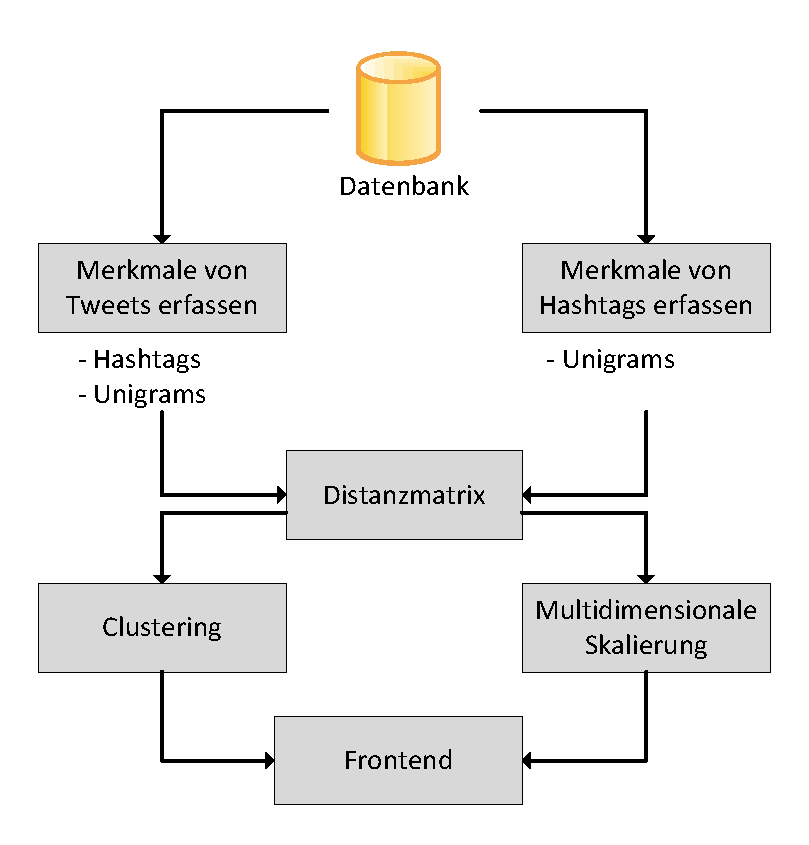
\includegraphics[scale=0.7]{./Bilder/Clustering/ClusteringAufbau.pdf}
\caption{Vorgehensweise bei der Cluster-Analyse}
\label{fig:ClusterVorgehen}
\end{figure}

Bei der Analyse von Tweets stellt die beschränkte Textlänge ein Problem dar, 
wodurch sich nur wenige Informationen extrahieren lassen. Daher wurden schrittweise 
verschiedene Ansätze zur Merkmalsextraktion implementiert, zum Beispiel die Erfassung der 
Hashtags oder der Wörter eines Tweets, auch Unigrams genannt. Diese Ansätze sind in Abschnitt \ref{subsec:ClusterTweets} beschrieben.
Zusätzlich erfolgt eine Cluster-Analyse der Hashtags, welches Kapitel \ref{subsec:ClusterHashtags} beschreibt. 
Hier lassen sich bei der Merkmalsextraktion eines Hashtags alle Tweets, die diesen Hashtag enthalten, heranziehen. 
Damit sind mehr Informationen vorhanden, um einzelne Hashtags zu gruppieren.
Kapitel \ref{subsec:ClusterTweetsWithHashtags} beschreibt einen zweistufigen Ansatz, 
welcher auf Basis der Hashtag"=Cluster versucht, Tweets zu gruppieren. 
Anschließend wird die Distanz der Objekte basierend auf den erhobenen Merkmalen berechnet. 
Mit dem Distanzmaß ist es nun möglich, die eigentliche Cluster"=Analyse 
durch\-zu\-füh\-ren (Kapitel \ref{subsec:ClusterAlgorithmen}). 
Gleichzeitig erfolgt eine Darstellung der Objekte im zweidimensionalen Raum, 
basierend auf den Distanzen (Kapitel \ref{subsec:MDS}). 
Die Cluster"=Zuordnungen sowie die Positionen im zweidimensionalen Raum werden 
anschließend dem Frontend zur grafischen Aufbereitung übergeben.
Das Kapitel schließt mit einer Diskussion der Ergebnisse und gibt einen Ausblick, 
welche Schritte in wei\-te\-ren Scrum"=Iterationen möglich gewesen wären.

%Erwin:
\subsection{Cluster-Analyse von Tweets} \label{subsec:ClusterTweets}

Aus Tweets lassen sich verschiedene Typen von Merkmalen ableiten, mit denen es möglich ist, 
Tweets nach ihrer gegenseitigen Ähnlichkeit zu bewerten. Diese Merkmalstypen werden im Folgenden anhand eines durchgehenden Beispiels erläutert:
\begin{itemize}
\item \textbf{Tweet 1:} \#CDU \#SPD Merkel ist in London
\item \textbf{Tweet 2:} \#CDU \#SPD Merkel reist nach London
\item \textbf{Tweet 3:} Merkel mag \#Rom.
\end{itemize}

%Erwin
\subsubsection{Hashtags als Merkmale}\label{subsec:HashtagsAlsMerkmale}
Die Erfassung der Hashtags eines Tweets stellt die erste Möglichkeit dar, Tweets gegenseitig zu bewerten. 
Da ein Tweet in der Regel keine Wiederholung von Hashtags enthält, 
zählt nur das Auftreten des Hashtags, nicht die Anzahl. 
Damit ist das Hashtag-Merkmal binärkodiert, wobei eine 1 für das Auftreten im Tweet steht. 
Im obigen Beispiel ergibt sich somit die Tabelle \ref{fig:ClusterTab1}. 
Die Zeilen stellen die Tweets dar, die Spalten die erhobenen Merkmale für die Cluster-Analyse.

\begin{table}[ht]
\centering
\begin{tabular}{cccc}
\toprule
 & \#CDU & \#SPD &  \#Rom \\ 
\midrule
Tweet~1 & 1 & 1  & 0 \\ 
 
Tweet~2 & 1 & 1  & 0 \\ 
 
Tweet~3 & 0 & 0  & 1 \\ 
\bottomrule 
\end{tabular} 
\caption{Binäre Merkmale eines Tweets: Hashtags}
\label{fig:ClusterTab1}
\end{table}

Dieses Beispiel erläutert auch die Idee hinter der Hashtag-Erfassung. 
Da Hashtags als Schlagwörter einen Tweet beschreiben, sollten zwei Tweets 
thematisch ähnlicher sein, je mehr übereinstimmende Hashtags sie besitzen.
Im vorliegenden Beispiel sind sich Tweet~1 und Tweet~2 ähnlicher, 
denn beide verwenden die Hashtags \glqq \#CDU\grqq{} und \glqq \#SPD\grqq{}. 

Die Ähnlichkeitserfassung hängt von der Datenskalierung ab. 
Da die Merkmale bi\-när\-ko\-diert sind, kommen Kennzahlen in Frage, 
die die Übereinstimmungen abzählen. Dabei kommen jedoch nur 
Ähnlichkeitsmaße in Frage, bei denen das gleiche Auftreten 
(eine 1er-Übereinstimmung bei jeweils zwei Tweets) eine Rolle spielt. 
Dementsprechend wurden die Ähnlichkeitsmaße Dice, S-Koeffizient, M-Koeffizient und Russel Rao in Betracht gezogen.

%Wladimir
Sei $n_{11}$ die Anzahl der gemeinsam aufgetretenen
Merkmale in zwei Tweets,  $n_{10}$ die Anzahl der Merkmale, die nur im ersten Tweet vorkommen,
$n_{01}$ die Anzahl der Merkmale, die nur im zweiten Tweet vorkommen und 
$n_{00}$ die Anzahl der Merkmale, die in den beiden Tweets nicht vorkommen, dann sind die genannten Ähnlichkeiten
zwi\-schen zwei Tweets wie folgt definiert:
\begin{align*}
& \frac{2n_{11}}{n_{01}+n_{10}+2n_{11}}, \tag{Dice} \\\\
& \frac{n_{11}}{n_{01}+n_{10}+n_{11}}, \tag{S-Koeffizient} \\\\
& \frac{n_{00}+n_{11}}{n_{00}+n_{01}+n_{10}+n_{11}}, \tag{M-Koeffizient}\\\\
& \frac{n_{11}}{n_{00}+n_{01}+n_{10}+n_{11}} \tag{Russel Rao}.
\end{align*}

%\subsection{Wahl der binären Ähnlichkeitsmaße}
%Für die Cluster-Analyse der Tweets mit Hilfe der Hashtags beziehungsweise der Wörter wurden binäre 
%Ahnlichkeitmaße verwendet, siehe Kapitel \ref{subsec:HashtagsAlsMerkmale} und \ref{subsec:WoerterAlsMerkmale}.
%Um einen besseren Eindruck von den unterschiedlichen Ähnlichkeitsmaßen zu bekommen, haben wir ihre Wirkung auf das Ergebnis
%getestet. Die Ähnlichkeitsmaße Dice, S-Koeffizient, M-Koeffizient und Russel Rao wurden in Betracht gezogen, 
%weil sie das gemeinsame Auftreten der Merkmale berücksichtigen. Sei $n_{11}$ die Anzahl der gemeinsam aufgetretenen
%Merkmale in zwei Tweets,  $n_{10}$ die Anzahl der Merkmale, die nur im ersten Tweet vorkamen,
%$n_{01}$ die Anzahl der Merkmale, die nur im zweiten Tweet vorkamen und 
%$n_{00}$ die Anzahl der Merkmale, die in den beiden Tweets nicht vorkamen, dann sind die genannten Ähnlichkeiten
%zwi\-schen zwei Tweets wie folgt definiert:
%\begin{align}
%\frac{2n_{11}}{n_{01}+n_{10}+2n_{11}}, \tag{Dice} \\
%\frac{n_{11}}{n_{01}+n_{10}+n_{11}}, \tag{S-Koeffizient} \\
%\frac{n_{00}+n_{11}}{p}, \tag{M-Koeffizient}\\
%\frac{n_{11}}{p} \tag{Russel Rao}.
%\end{align}

% \def\myDissScale{0.33}
% \begin{figure}[ht]
%    \centering
%       \subcaptionbox{Dice\label{img:Dice}}{\def\maxW{4.23}
\begin{tikzpicture}[scale=\textwidth*\myDissScale/1.0cm, background rectangle/.style={draw=black, thick, fill=yellow!10,},show background rectangle]
\def\marRad{0.20}
\definecolor{color0}{rgb}{0.78,0.89,0.11}
\definecolor{color1}{rgb}{0.10,1.00,0.52}
\definecolor{color2}{rgb}{0.09,0.32,0.64}
\definecolor{color3}{rgb}{0.70,0.69,0.42}
\definecolor{color4}{rgb}{0.36,0.70,0.25}
\definecolor{color5}{rgb}{0.91,0.34,0.56}
\definecolor{color6}{rgb}{0.76,0.33,0.65}
\definecolor{color7}{rgb}{0.06,0.22,0.62}
\definecolor{color8}{rgb}{0.45,0.68,0.87}
\definecolor{color9}{rgb}{0.03,0.89,0.67}
\path[fill=color0,draw=color0,mark size=\marRad, mark=*] plot coordinates {(0.09, -0.43)};
\path[fill=color0,draw=color0,mark size=\marRad, mark=*] plot coordinates {(-0.20, -0.09)};
\path[fill=color0,draw=color0,mark size=\marRad, mark=*] plot coordinates {(-0.03, -0.44)};
\path[fill=color0,draw=color0,mark size=\marRad, mark=*] plot coordinates {(0.41, -0.10)};
\path[fill=color0,draw=color0,mark size=\marRad, mark=*] plot coordinates {(0.11, -0.28)};
\path[fill=color0,draw=color0,mark size=\marRad, mark=*] plot coordinates {(-0.33, -0.14)};
\path[fill=color0,draw=color0,mark size=\marRad, mark=*] plot coordinates {(-0.08, -0.26)};
\path[fill=color0,draw=color0,mark size=\marRad, mark=*] plot coordinates {(0.41, -0.19)};
\path[fill=color0,draw=color0,mark size=\marRad, mark=*] plot coordinates {(0.22, -0.21)};
\path[fill=color0,draw=color0,mark size=\marRad, mark=*] plot coordinates {(-0.28, -0.28)};
\path[fill=color0,draw=color0,mark size=\marRad, mark=*] plot coordinates {(0.41, 0.11)};
\path[fill=color0,draw=color0,mark size=\marRad, mark=*] plot coordinates {(0.43, -0.19)};
\path[fill=color0,draw=color0,mark size=\marRad, mark=*] plot coordinates {(-0.24, -0.03)};
\path[fill=color0,draw=color0,mark size=\marRad, mark=*] plot coordinates {(-0.42, -0.16)};
\path[fill=color0,draw=color0,mark size=\marRad, mark=*] plot coordinates {(-0.25, -0.15)};
\path[fill=color0,draw=color0,mark size=\marRad, mark=*] plot coordinates {(-0.24, -0.15)};
\path[fill=color0,draw=color0,mark size=\marRad, mark=*] plot coordinates {(0.02, -0.41)};
\path[fill=color0,draw=color0,mark size=\marRad, mark=*] plot coordinates {(0.23, -0.01)};
\path[fill=color0,draw=color0,mark size=\marRad, mark=*] plot coordinates {(-0.14, -0.09)};
\path[fill=color0,draw=color0,mark size=\marRad, mark=*] plot coordinates {(0.01, -0.26)};
\path[fill=color0,draw=color0,mark size=\marRad, mark=*] plot coordinates {(0.33, 0.29)};
\path[fill=color0,draw=color0,mark size=\marRad, mark=*] plot coordinates {(0.16, -0.27)};
\path[fill=color0,draw=color0,mark size=\marRad, mark=*] plot coordinates {(0.37, 0.20)};
\path[fill=color0,draw=color0,mark size=\marRad, mark=*] plot coordinates {(-0.41, -0.17)};
\path[fill=color0,draw=color0,mark size=\marRad, mark=*] plot coordinates {(0.33, 0.16)};
\path[fill=color0,draw=color0,mark size=\marRad, mark=*] plot coordinates {(0.25, -0.30)};
\path[fill=color0,draw=color0,mark size=\marRad, mark=*] plot coordinates {(-0.10, -0.22)};
\path[fill=color0,draw=color0,mark size=\marRad, mark=*] plot coordinates {(-0.24, 0.03)};
\path[fill=color0,draw=color0,mark size=\marRad, mark=*] plot coordinates {(0.13, 0.21)};
\path[fill=color0,draw=color0,mark size=\marRad, mark=*] plot coordinates {(0.07, -0.42)};
\path[fill=color0,draw=color0,mark size=\marRad, mark=*] plot coordinates {(0.47, -0.09)};
\path[fill=color0,draw=color0,mark size=\marRad, mark=*] plot coordinates {(0.34, -0.32)};
\path[fill=color0,draw=color0,mark size=\marRad, mark=*] plot coordinates {(0.44, 0.02)};
\path[fill=color0,draw=color0,mark size=\marRad, mark=*] plot coordinates {(0.37, -0.29)};
\path[fill=color0,draw=color0,mark size=\marRad, mark=*] plot coordinates {(-0.08, 0.07)};
\path[fill=color0,draw=color0,mark size=\marRad, mark=*] plot coordinates {(0.09, -0.14)};
\path[fill=color0,draw=color0,mark size=\marRad, mark=*] plot coordinates {(-0.22, -0.13)};
\path[fill=color0,draw=color0,mark size=\marRad, mark=*] plot coordinates {(-0.22, -0.22)};
\path[fill=color0,draw=color0,mark size=\marRad, mark=*] plot coordinates {(0.44, 0.11)};
\path[fill=color0,draw=color0,mark size=\marRad, mark=*] plot coordinates {(0.02, 0.13)};
\path[fill=color0,draw=color0,mark size=\marRad, mark=*] plot coordinates {(-0.17, -0.28)};
\path[fill=color0,draw=color0,mark size=\marRad, mark=*] plot coordinates {(-0.31, 0.01)};
\path[fill=color0,draw=color0,mark size=\marRad, mark=*] plot coordinates {(0.07, -0.22)};
\path[fill=color0,draw=color0,mark size=\marRad, mark=*] plot coordinates {(0.15, -0.42)};
\path[fill=color0,draw=color0,mark size=\marRad, mark=*] plot coordinates {(-0.24, -0.17)};
\path[fill=color0,draw=color0,mark size=\marRad, mark=*] plot coordinates {(0.12, -0.03)};
\path[fill=color0,draw=color0,mark size=\marRad, mark=*] plot coordinates {(-0.19, -0.04)};
\path[fill=color0,draw=color0,mark size=\marRad, mark=*] plot coordinates {(0.10, 0.15)};
\path[fill=color0,draw=color0,mark size=\marRad, mark=*] plot coordinates {(0.39, -0.09)};
\path[fill=color0,draw=color0,mark size=\marRad, mark=*] plot coordinates {(0.33, 0.17)};
\path[fill=color0,draw=color0,mark size=\marRad, mark=*] plot coordinates {(-0.09, -0.23)};
\path[fill=color0,draw=color0,mark size=\marRad, mark=*] plot coordinates {(0.44, 0.04)};
\path[fill=color0,draw=color0,mark size=\marRad, mark=*] plot coordinates {(0.04, 0.03)};
\path[fill=color0,draw=color0,mark size=\marRad, mark=*] plot coordinates {(0.28, -0.31)};
\path[fill=color0,draw=color0,mark size=\marRad, mark=*] plot coordinates {(-0.11, 0.00)};
\path[fill=color0,draw=color0,mark size=\marRad, mark=*] plot coordinates {(0.39, -0.00)};
\path[fill=color0,draw=color0,mark size=\marRad, mark=*] plot coordinates {(0.05, -0.43)};
\path[fill=color0,draw=color0,mark size=\marRad, mark=*] plot coordinates {(-0.03, -0.01)};
\path[fill=color0,draw=color0,mark size=\marRad, mark=*] plot coordinates {(0.24, -0.36)};
\path[fill=color0,draw=color0,mark size=\marRad, mark=*] plot coordinates {(0.07, -0.14)};
\path[fill=color0,draw=color0,mark size=\marRad, mark=*] plot coordinates {(-0.17, -0.20)};
\path[fill=color0,draw=color0,mark size=\marRad, mark=*] plot coordinates {(0.43, -0.21)};
\path[fill=color0,draw=color0,mark size=\marRad, mark=*] plot coordinates {(0.09, -0.19)};
\path[fill=color0,draw=color0,mark size=\marRad, mark=*] plot coordinates {(0.25, -0.34)};
\path[fill=color0,draw=color0,mark size=\marRad, mark=*] plot coordinates {(0.46, 0.12)};
\path[fill=color0,draw=color0,mark size=\marRad, mark=*] plot coordinates {(0.22, -0.18)};
\path[fill=color0,draw=color0,mark size=\marRad, mark=*] plot coordinates {(0.10, 0.02)};
\path[fill=color0,draw=color0,mark size=\marRad, mark=*] plot coordinates {(-0.39, -0.11)};
\path[fill=color0,draw=color0,mark size=\marRad, mark=*] plot coordinates {(0.37, -0.15)};
\path[fill=color0,draw=color0,mark size=\marRad, mark=*] plot coordinates {(0.19, -0.30)};
\path[fill=color0,draw=color0,mark size=\marRad, mark=*] plot coordinates {(-0.01, -0.10)};
\path[fill=color0,draw=color0,mark size=\marRad, mark=*] plot coordinates {(0.16, -0.30)};
\path[fill=color0,draw=color0,mark size=\marRad, mark=*] plot coordinates {(0.34, -0.25)};
\path[fill=color0,draw=color0,mark size=\marRad, mark=*] plot coordinates {(0.32, 0.30)};
\path[fill=color0,draw=color0,mark size=\marRad, mark=*] plot coordinates {(0.31, 0.25)};
\path[fill=color0,draw=color0,mark size=\marRad, mark=*] plot coordinates {(-0.34, -0.15)};
\path[fill=color0,draw=color0,mark size=\marRad, mark=*] plot coordinates {(0.35, 0.02)};
\path[fill=color0,draw=color0,mark size=\marRad, mark=*] plot coordinates {(-0.37, 0.05)};
\path[fill=color0,draw=color0,mark size=\marRad, mark=*] plot coordinates {(0.25, -0.23)};
\path[fill=color0,draw=color0,mark size=\marRad, mark=*] plot coordinates {(0.16, 0.04)};
\path[fill=color0,draw=color0,mark size=\marRad, mark=*] plot coordinates {(0.39, 0.29)};
\path[fill=color0,draw=color0,mark size=\marRad, mark=*] plot coordinates {(0.05, 0.13)};
\path[fill=color0,draw=color0,mark size=\marRad, mark=*] plot coordinates {(-0.32, -0.20)};
\path[fill=color0,draw=color0,mark size=\marRad, mark=*] plot coordinates {(0.32, 0.11)};
\path[fill=color0,draw=color0,mark size=\marRad, mark=*] plot coordinates {(0.38, -0.06)};
\path[fill=color0,draw=color0,mark size=\marRad, mark=*] plot coordinates {(0.42, 0.01)};
\path[fill=color0,draw=color0,mark size=\marRad, mark=*] plot coordinates {(0.32, -0.12)};
\path[fill=color0,draw=color0,mark size=\marRad, mark=*] plot coordinates {(0.29, -0.17)};
\path[fill=color0,draw=color0,mark size=\marRad, mark=*] plot coordinates {(0.17, -0.25)};
\path[fill=color0,draw=color0,mark size=\marRad, mark=*] plot coordinates {(0.33, 0.20)};
\path[fill=color0,draw=color0,mark size=\marRad, mark=*] plot coordinates {(-0.06, -0.03)};
\path[fill=color0,draw=color0,mark size=\marRad, mark=*] plot coordinates {(-0.01, -0.04)};
\path[fill=color0,draw=color0,mark size=\marRad, mark=*] plot coordinates {(0.43, 0.08)};
\path[fill=color0,draw=color0,mark size=\marRad, mark=*] plot coordinates {(-0.34, -0.18)};
\path[fill=color0,draw=color0,mark size=\marRad, mark=*] plot coordinates {(0.39, 0.00)};
\path[fill=color0,draw=color0,mark size=\marRad, mark=*] plot coordinates {(0.17, -0.15)};
\path[fill=color0,draw=color0,mark size=\marRad, mark=*] plot coordinates {(-0.09, -0.11)};
\path[fill=color0,draw=color0,mark size=\marRad, mark=*] plot coordinates {(0.46, 0.07)};
\path[fill=color0,draw=color0,mark size=\marRad, mark=*] plot coordinates {(-0.17, 0.01)};
\path[fill=color0,draw=color0,mark size=\marRad, mark=*] plot coordinates {(0.25, -0.16)};
\path[fill=color0,draw=color0,mark size=\marRad, mark=*] plot coordinates {(0.01, -0.21)};
\path[fill=color0,draw=color0,mark size=\marRad, mark=*] plot coordinates {(0.33, -0.01)};
\path[fill=color0,draw=color0,mark size=\marRad, mark=*] plot coordinates {(0.07, -0.34)};
\path[fill=color0,draw=color0,mark size=\marRad, mark=*] plot coordinates {(-0.20, -0.00)};
\path[fill=color0,draw=color0,mark size=\marRad, mark=*] plot coordinates {(0.02, -0.35)};
\path[fill=color0,draw=color0,mark size=\marRad, mark=*] plot coordinates {(0.39, -0.13)};
\path[fill=color0,draw=color0,mark size=\marRad, mark=*] plot coordinates {(-0.20, -0.24)};
\path[fill=color0,draw=color0,mark size=\marRad, mark=*] plot coordinates {(0.11, -0.44)};
\path[fill=color0,draw=color0,mark size=\marRad, mark=*] plot coordinates {(0.46, -0.01)};
\path[fill=color0,draw=color0,mark size=\marRad, mark=*] plot coordinates {(0.26, -0.39)};
\path[fill=color0,draw=color0,mark size=\marRad, mark=*] plot coordinates {(-0.17, -0.35)};
\path[fill=color0,draw=color0,mark size=\marRad, mark=*] plot coordinates {(-0.26, 0.05)};
\path[fill=color0,draw=color0,mark size=\marRad, mark=*] plot coordinates {(-0.08, -0.41)};
\path[fill=color0,draw=color0,mark size=\marRad, mark=*] plot coordinates {(0.28, -0.25)};
\path[fill=color0,draw=color0,mark size=\marRad, mark=*] plot coordinates {(-0.19, -0.17)};
\path[fill=color0,draw=color0,mark size=\marRad, mark=*] plot coordinates {(0.28, -0.11)};
\path[fill=color0,draw=color0,mark size=\marRad, mark=*] plot coordinates {(-0.01, -0.01)};
\path[fill=color0,draw=color0,mark size=\marRad, mark=*] plot coordinates {(-0.01, 0.08)};
\path[fill=color0,draw=color0,mark size=\marRad, mark=*] plot coordinates {(0.20, 0.13)};
\path[fill=color0,draw=color0,mark size=\marRad, mark=*] plot coordinates {(0.49, 0.02)};
\path[fill=color0,draw=color0,mark size=\marRad, mark=*] plot coordinates {(0.22, -0.42)};
\path[fill=color0,draw=color0,mark size=\marRad, mark=*] plot coordinates {(0.35, -0.19)};
\path[fill=color0,draw=color0,mark size=\marRad, mark=*] plot coordinates {(-0.07, 0.04)};
\path[fill=color0,draw=color0,mark size=\marRad, mark=*] plot coordinates {(0.30, -0.29)};
\path[fill=color0,draw=color0,mark size=\marRad, mark=*] plot coordinates {(0.11, 0.11)};
\path[fill=color0,draw=color0,mark size=\marRad, mark=*] plot coordinates {(0.29, 0.16)};
\path[fill=color0,draw=color0,mark size=\marRad, mark=*] plot coordinates {(0.44, 0.21)};
\path[fill=color0,draw=color0,mark size=\marRad, mark=*] plot coordinates {(-0.35, -0.10)};
\path[fill=color0,draw=color0,mark size=\marRad, mark=*] plot coordinates {(0.29, -0.38)};
\path[fill=color0,draw=color0,mark size=\marRad, mark=*] plot coordinates {(0.28, 0.10)};
\path[fill=color0,draw=color0,mark size=\marRad, mark=*] plot coordinates {(0.33, -0.14)};
\path[fill=color0,draw=color0,mark size=\marRad, mark=*] plot coordinates {(0.40, -0.28)};
\path[fill=color0,draw=color0,mark size=\marRad, mark=*] plot coordinates {(0.23, 0.11)};
\path[fill=color0,draw=color0,mark size=\marRad, mark=*] plot coordinates {(-0.18, -0.29)};
\path[fill=color0,draw=color0,mark size=\marRad, mark=*] plot coordinates {(0.17, -0.01)};
\path[fill=color0,draw=color0,mark size=\marRad, mark=*] plot coordinates {(0.10, -0.47)};
\path[fill=color0,draw=color0,mark size=\marRad, mark=*] plot coordinates {(0.33, -0.06)};
\path[fill=color0,draw=color0,mark size=\marRad, mark=*] plot coordinates {(0.09, -0.26)};
\path[fill=color0,draw=color0,mark size=\marRad, mark=*] plot coordinates {(0.36, 0.04)};
\path[fill=color0,draw=color0,mark size=\marRad, mark=*] plot coordinates {(0.33, -0.02)};
\path[fill=color0,draw=color0,mark size=\marRad, mark=*] plot coordinates {(0.15, -0.36)};
\path[fill=color0,draw=color0,mark size=\marRad, mark=*] plot coordinates {(0.45, -0.06)};
\path[fill=color0,draw=color0,mark size=\marRad, mark=*] plot coordinates {(-0.27, -0.11)};
\path[fill=color0,draw=color0,mark size=\marRad, mark=*] plot coordinates {(0.43, 0.08)};
\path[fill=color0,draw=color0,mark size=\marRad, mark=*] plot coordinates {(-0.38, -0.25)};
\path[fill=color0,draw=color0,mark size=\marRad, mark=*] plot coordinates {(0.27, -0.40)};
\path[fill=color0,draw=color0,mark size=\marRad, mark=*] plot coordinates {(0.16, -0.40)};
\path[fill=color0,draw=color0,mark size=\marRad, mark=*] plot coordinates {(-0.30, -0.27)};
\path[fill=color0,draw=color0,mark size=\marRad, mark=*] plot coordinates {(0.10, -0.45)};
\path[fill=color0,draw=color0,mark size=\marRad, mark=*] plot coordinates {(0.37, 0.05)};
\path[fill=color0,draw=color0,mark size=\marRad, mark=*] plot coordinates {(0.15, -0.40)};
\path[fill=color0,draw=color0,mark size=\marRad, mark=*] plot coordinates {(-0.04, -0.14)};
\path[fill=color0,draw=color0,mark size=\marRad, mark=*] plot coordinates {(0.46, 0.06)};
\path[fill=color0,draw=color0,mark size=\marRad, mark=*] plot coordinates {(0.37, 0.30)};
\path[fill=color0,draw=color0,mark size=\marRad, mark=*] plot coordinates {(0.34, 0.09)};
\path[fill=color0,draw=color0,mark size=\marRad, mark=*] plot coordinates {(-0.04, 0.09)};
\path[fill=color0,draw=color0,mark size=\marRad, mark=*] plot coordinates {(0.41, -0.06)};
\path[fill=color0,draw=color0,mark size=\marRad, mark=*] plot coordinates {(0.35, -0.25)};
\path[fill=color0,draw=color0,mark size=\marRad, mark=*] plot coordinates {(-0.13, -0.17)};
\path[fill=color0,draw=color0,mark size=\marRad, mark=*] plot coordinates {(0.41, -0.12)};
\path[fill=color0,draw=color0,mark size=\marRad, mark=*] plot coordinates {(0.18, -0.41)};
\path[fill=color0,draw=color0,mark size=\marRad, mark=*] plot coordinates {(-0.09, -0.03)};
\path[fill=color0,draw=color0,mark size=\marRad, mark=*] plot coordinates {(0.01, -0.46)};
\path[fill=color0,draw=color0,mark size=\marRad, mark=*] plot coordinates {(0.35, -0.16)};
\path[fill=color0,draw=color0,mark size=\marRad, mark=*] plot coordinates {(0.24, 0.13)};
\path[fill=color0,draw=color0,mark size=\marRad, mark=*] plot coordinates {(0.25, 0.20)};
\path[fill=color0,draw=color0,mark size=\marRad, mark=*] plot coordinates {(0.42, 0.14)};
\path[fill=color0,draw=color0,mark size=\marRad, mark=*] plot coordinates {(0.36, -0.04)};
\path[fill=color0,draw=color0,mark size=\marRad, mark=*] plot coordinates {(0.11, -0.13)};
\path[fill=color0,draw=color0,mark size=\marRad, mark=*] plot coordinates {(0.09, -0.07)};
\path[fill=color0,draw=color0,mark size=\marRad, mark=*] plot coordinates {(-0.19, -0.37)};
\path[fill=color0,draw=color0,mark size=\marRad, mark=*] plot coordinates {(0.17, 0.03)};
\path[fill=color0,draw=color0,mark size=\marRad, mark=*] plot coordinates {(0.20, -0.35)};
\path[fill=color0,draw=color0,mark size=\marRad, mark=*] plot coordinates {(0.29, 0.09)};
\path[fill=color0,draw=color0,mark size=\marRad, mark=*] plot coordinates {(0.45, -0.18)};
\path[fill=color0,draw=color0,mark size=\marRad, mark=*] plot coordinates {(0.44, 0.04)};
\path[fill=color0,draw=color0,mark size=\marRad, mark=*] plot coordinates {(0.35, -0.12)};
\path[fill=color0,draw=color0,mark size=\marRad, mark=*] plot coordinates {(0.39, 0.26)};
\path[fill=color0,draw=color0,mark size=\marRad, mark=*] plot coordinates {(-0.23, -0.33)};
\path[fill=color0,draw=color0,mark size=\marRad, mark=*] plot coordinates {(-0.04, -0.16)};
\path[fill=color0,draw=color0,mark size=\marRad, mark=*] plot coordinates {(0.33, -0.31)};
\path[fill=color0,draw=color0,mark size=\marRad, mark=*] plot coordinates {(0.42, -0.05)};
\path[fill=color0,draw=color0,mark size=\marRad, mark=*] plot coordinates {(-0.01, -0.15)};
\path[fill=color0,draw=color0,mark size=\marRad, mark=*] plot coordinates {(0.46, -0.10)};
\path[fill=color0,draw=color0,mark size=\marRad, mark=*] plot coordinates {(0.24, -0.22)};
\path[fill=color0,draw=color0,mark size=\marRad, mark=*] plot coordinates {(0.12, -0.22)};
\path[fill=color0,draw=color0,mark size=\marRad, mark=*] plot coordinates {(-0.16, -0.43)};
\path[fill=color0,draw=color0,mark size=\marRad, mark=*] plot coordinates {(0.35, -0.34)};
\path[fill=color0,draw=color0,mark size=\marRad, mark=*] plot coordinates {(0.45, -0.18)};
\path[fill=color0,draw=color0,mark size=\marRad, mark=*] plot coordinates {(-0.13, -0.19)};
\path[fill=color0,draw=color0,mark size=\marRad, mark=*] plot coordinates {(0.02, 0.10)};
\path[fill=color0,draw=color0,mark size=\marRad, mark=*] plot coordinates {(0.13, 0.05)};
\path[fill=color0,draw=color0,mark size=\marRad, mark=*] plot coordinates {(0.12, -0.38)};
\path[fill=color0,draw=color0,mark size=\marRad, mark=*] plot coordinates {(0.19, -0.42)};
\path[fill=color0,draw=color0,mark size=\marRad, mark=*] plot coordinates {(0.19, -0.13)};
\path[fill=color0,draw=color0,mark size=\marRad, mark=*] plot coordinates {(0.19, -0.42)};
\path[fill=color0,draw=color0,mark size=\marRad, mark=*] plot coordinates {(-0.36, 0.03)};
\path[fill=color0,draw=color0,mark size=\marRad, mark=*] plot coordinates {(-0.30, -0.03)};
\path[fill=color0,draw=color0,mark size=\marRad, mark=*] plot coordinates {(0.47, -0.09)};
\path[fill=color0,draw=color0,mark size=\marRad, mark=*] plot coordinates {(0.31, -0.37)};
\path[fill=color0,draw=color0,mark size=\marRad, mark=*] plot coordinates {(0.38, 0.06)};
\path[fill=color0,draw=color0,mark size=\marRad, mark=*] plot coordinates {(-0.33, -0.19)};
\path[fill=color0,draw=color0,mark size=\marRad, mark=*] plot coordinates {(-0.08, -0.45)};
\path[fill=color0,draw=color0,mark size=\marRad, mark=*] plot coordinates {(0.16, -0.30)};
\path[fill=color0,draw=color0,mark size=\marRad, mark=*] plot coordinates {(-0.03, -0.24)};
\path[fill=color0,draw=color0,mark size=\marRad, mark=*] plot coordinates {(-0.06, -0.36)};
\path[fill=color0,draw=color0,mark size=\marRad, mark=*] plot coordinates {(0.44, 0.19)};
\path[fill=color0,draw=color0,mark size=\marRad, mark=*] plot coordinates {(0.06, -0.20)};
\path[fill=color0,draw=color0,mark size=\marRad, mark=*] plot coordinates {(-0.33, -0.03)};
\path[fill=color0,draw=color0,mark size=\marRad, mark=*] plot coordinates {(-0.24, -0.37)};
\path[fill=color0,draw=color0,mark size=\marRad, mark=*] plot coordinates {(0.01, -0.08)};
\path[fill=color0,draw=color0,mark size=\marRad, mark=*] plot coordinates {(0.21, -0.24)};
\path[fill=color0,draw=color0,mark size=\marRad, mark=*] plot coordinates {(0.24, -0.40)};
\path[fill=color0,draw=color0,mark size=\marRad, mark=*] plot coordinates {(0.36, 0.26)};
\path[fill=color0,draw=color0,mark size=\marRad, mark=*] plot coordinates {(-0.14, 0.04)};
\path[fill=color0,draw=color0,mark size=\marRad, mark=*] plot coordinates {(-0.01, -0.43)};
\path[fill=color0,draw=color0,mark size=\marRad, mark=*] plot coordinates {(-0.25, -0.24)};
\path[fill=color0,draw=color0,mark size=\marRad, mark=*] plot coordinates {(0.26, -0.29)};
\path[fill=color0,draw=color0,mark size=\marRad, mark=*] plot coordinates {(0.01, -0.31)};
\path[fill=color0,draw=color0,mark size=\marRad, mark=*] plot coordinates {(0.36, 0.21)};
\path[fill=color0,draw=color0,mark size=\marRad, mark=*] plot coordinates {(0.22, -0.20)};
\path[fill=color0,draw=color0,mark size=\marRad, mark=*] plot coordinates {(-0.03, -0.21)};
\path[fill=color0,draw=color0,mark size=\marRad, mark=*] plot coordinates {(-0.18, -0.28)};
\path[fill=color0,draw=color0,mark size=\marRad, mark=*] plot coordinates {(0.48, 0.09)};
\path[fill=color0,draw=color0,mark size=\marRad, mark=*] plot coordinates {(-0.22, -0.11)};
\path[fill=color0,draw=color0,mark size=\marRad, mark=*] plot coordinates {(0.37, -0.23)};
\path[fill=color0,draw=color0,mark size=\marRad, mark=*] plot coordinates {(-0.41, 0.03)};
\path[fill=color0,draw=color0,mark size=\marRad, mark=*] plot coordinates {(0.01, -0.23)};
\path[fill=color0,draw=color0,mark size=\marRad, mark=*] plot coordinates {(0.20, 0.17)};
\path[fill=color0,draw=color0,mark size=\marRad, mark=*] plot coordinates {(-0.04, -0.22)};
\path[fill=color0,draw=color0,mark size=\marRad, mark=*] plot coordinates {(-0.39, -0.00)};
\path[fill=color0,draw=color0,mark size=\marRad, mark=*] plot coordinates {(-0.26, -0.05)};
\path[fill=color0,draw=color0,mark size=\marRad, mark=*] plot coordinates {(0.45, -0.14)};
\path[fill=color0,draw=color0,mark size=\marRad, mark=*] plot coordinates {(-0.33, -0.27)};
\path[fill=color0,draw=color0,mark size=\marRad, mark=*] plot coordinates {(0.19, 0.11)};
\path[fill=color0,draw=color0,mark size=\marRad, mark=*] plot coordinates {(0.35, -0.30)};
\path[fill=color0,draw=color0,mark size=\marRad, mark=*] plot coordinates {(-0.19, 0.01)};
\path[fill=color0,draw=color0,mark size=\marRad, mark=*] plot coordinates {(0.34, -0.34)};
\path[fill=color0,draw=color0,mark size=\marRad, mark=*] plot coordinates {(0.31, -0.28)};
\path[fill=color0,draw=color0,mark size=\marRad, mark=*] plot coordinates {(0.25, -0.14)};
\path[fill=color0,draw=color0,mark size=\marRad, mark=*] plot coordinates {(0.28, -0.07)};
\path[fill=color0,draw=color0,mark size=\marRad, mark=*] plot coordinates {(0.28, -0.33)};
\path[fill=color0,draw=color0,mark size=\marRad, mark=*] plot coordinates {(0.34, -0.07)};
\path[fill=color0,draw=color0,mark size=\marRad, mark=*] plot coordinates {(0.29, -0.20)};
\path[fill=color0,draw=color0,mark size=\marRad, mark=*] plot coordinates {(-0.15, -0.05)};
\path[fill=color0,draw=color0,mark size=\marRad, mark=*] plot coordinates {(-0.40, -0.04)};
\path[fill=color0,draw=color0,mark size=\marRad, mark=*] plot coordinates {(-0.14, -0.30)};
\path[fill=color0,draw=color0,mark size=\marRad, mark=*] plot coordinates {(0.20, 0.06)};
\path[fill=color0,draw=color0,mark size=\marRad, mark=*] plot coordinates {(0.46, 0.17)};
\path[fill=color0,draw=color0,mark size=\marRad, mark=*] plot coordinates {(-0.05, -0.20)};
\path[fill=color0,draw=color0,mark size=\marRad, mark=*] plot coordinates {(0.13, -0.14)};
\path[fill=color0,draw=color0,mark size=\marRad, mark=*] plot coordinates {(0.28, -0.13)};
\path[fill=color0,draw=color0,mark size=\marRad, mark=*] plot coordinates {(0.15, 0.06)};
\path[fill=color0,draw=color0,mark size=\marRad, mark=*] plot coordinates {(0.22, -0.16)};
\path[fill=color0,draw=color0,mark size=\marRad, mark=*] plot coordinates {(0.02, -0.04)};
\path[fill=color0,draw=color0,mark size=\marRad, mark=*] plot coordinates {(-0.02, -0.05)};
\path[fill=color0,draw=color0,mark size=\marRad, mark=*] plot coordinates {(0.31, 0.11)};
\path[fill=color0,draw=color0,mark size=\marRad, mark=*] plot coordinates {(0.10, 0.01)};
\path[fill=color0,draw=color0,mark size=\marRad, mark=*] plot coordinates {(0.21, -0.09)};
\path[fill=color0,draw=color0,mark size=\marRad, mark=*] plot coordinates {(0.21, -0.10)};
\path[fill=color0,draw=color0,mark size=\marRad, mark=*] plot coordinates {(0.24, -0.02)};
\path[fill=color0,draw=color0,mark size=\marRad, mark=*] plot coordinates {(0.30, 0.13)};
\path[fill=color0,draw=color0,mark size=\marRad, mark=*] plot coordinates {(0.03, -0.14)};
\path[fill=color0,draw=color0,mark size=\marRad, mark=*] plot coordinates {(-0.23, -0.08)};
\path[fill=color0,draw=color0,mark size=\marRad, mark=*] plot coordinates {(-0.03, -0.17)};
\path[fill=color0,draw=color0,mark size=\marRad, mark=*] plot coordinates {(0.11, -0.38)};
\path[fill=color0,draw=color0,mark size=\marRad, mark=*] plot coordinates {(-0.23, -0.28)};
\path[fill=color0,draw=color0,mark size=\marRad, mark=*] plot coordinates {(-0.17, -0.15)};
\path[fill=color0,draw=color0,mark size=\marRad, mark=*] plot coordinates {(0.13, -0.20)};
\path[fill=color0,draw=color0,mark size=\marRad, mark=*] plot coordinates {(-0.44, -0.10)};
\path[fill=color0,draw=color0,mark size=\marRad, mark=*] plot coordinates {(0.38, 0.13)};
\path[fill=color0,draw=color0,mark size=\marRad, mark=*] plot coordinates {(0.12, -0.13)};
\path[fill=color0,draw=color0,mark size=\marRad, mark=*] plot coordinates {(0.43, 0.17)};
\path[fill=color0,draw=color0,mark size=\marRad, mark=*] plot coordinates {(0.37, 0.19)};
\path[fill=color0,draw=color0,mark size=\marRad, mark=*] plot coordinates {(-0.22, -0.00)};
\path[fill=color0,draw=color0,mark size=\marRad, mark=*] plot coordinates {(-0.14, -0.18)};
\path[fill=color0,draw=color0,mark size=\marRad, mark=*] plot coordinates {(-0.38, -0.10)};
\path[fill=color0,draw=color0,mark size=\marRad, mark=*] plot coordinates {(-0.19, -0.04)};
\path[fill=color0,draw=color0,mark size=\marRad, mark=*] plot coordinates {(0.02, -0.16)};
\path[fill=color0,draw=color0,mark size=\marRad, mark=*] plot coordinates {(0.26, 0.12)};
\path[fill=color0,draw=color0,mark size=\marRad, mark=*] plot coordinates {(-0.03, -0.30)};
\path[fill=color0,draw=color0,mark size=\marRad, mark=*] plot coordinates {(0.19, -0.34)};
\path[fill=color0,draw=color0,mark size=\marRad, mark=*] plot coordinates {(0.03, -0.10)};
\path[fill=color0,draw=color0,mark size=\marRad, mark=*] plot coordinates {(0.40, 0.07)};
\path[fill=color0,draw=color0,mark size=\marRad, mark=*] plot coordinates {(-0.12, 0.10)};
\path[fill=color0,draw=color0,mark size=\marRad, mark=*] plot coordinates {(-0.01, -0.15)};
\path[fill=color0,draw=color0,mark size=\marRad, mark=*] plot coordinates {(-0.09, -0.32)};
\path[fill=color0,draw=color0,mark size=\marRad, mark=*] plot coordinates {(0.13, 0.22)};
\path[fill=color0,draw=color0,mark size=\marRad, mark=*] plot coordinates {(0.31, -0.39)};
\path[fill=color0,draw=color0,mark size=\marRad, mark=*] plot coordinates {(0.06, -0.16)};
\path[fill=color0,draw=color0,mark size=\marRad, mark=*] plot coordinates {(-0.40, -0.00)};
\path[fill=color0,draw=color0,mark size=\marRad, mark=*] plot coordinates {(0.39, 0.18)};
\path[fill=color0,draw=color0,mark size=\marRad, mark=*] plot coordinates {(0.16, -0.05)};
\path[fill=color0,draw=color0,mark size=\marRad, mark=*] plot coordinates {(-0.42, -0.07)};
\path[fill=color0,draw=color0,mark size=\marRad, mark=*] plot coordinates {(-0.44, -0.16)};
\path[fill=color0,draw=color0,mark size=\marRad, mark=*] plot coordinates {(0.07, -0.25)};
\path[fill=color0,draw=color0,mark size=\marRad, mark=*] plot coordinates {(0.06, -0.35)};
\path[fill=color0,draw=color0,mark size=\marRad, mark=*] plot coordinates {(-0.21, -0.27)};
\path[fill=color0,draw=color0,mark size=\marRad, mark=*] plot coordinates {(0.39, -0.10)};
\path[fill=color0,draw=color0,mark size=\marRad, mark=*] plot coordinates {(0.09, 0.11)};
\path[fill=color0,draw=color0,mark size=\marRad, mark=*] plot coordinates {(0.18, 0.07)};
\path[fill=color0,draw=color0,mark size=\marRad, mark=*] plot coordinates {(-0.13, -0.34)};
\path[fill=color0,draw=color0,mark size=\marRad, mark=*] plot coordinates {(0.16, -0.02)};
\path[fill=color0,draw=color0,mark size=\marRad, mark=*] plot coordinates {(0.23, 0.24)};
\path[fill=color0,draw=color0,mark size=\marRad, mark=*] plot coordinates {(0.35, -0.08)};
\path[fill=color0,draw=color0,mark size=\marRad, mark=*] plot coordinates {(0.34, -0.14)};
\path[fill=color0,draw=color0,mark size=\marRad, mark=*] plot coordinates {(0.39, 0.28)};
\path[fill=color0,draw=color0,mark size=\marRad, mark=*] plot coordinates {(-0.02, 0.12)};
\path[fill=color0,draw=color0,mark size=\marRad, mark=*] plot coordinates {(0.01, -0.49)};
\path[fill=color0,draw=color0,mark size=\marRad, mark=*] plot coordinates {(0.11, -0.04)};
\path[fill=color0,draw=color0,mark size=\marRad, mark=*] plot coordinates {(-0.42, 0.01)};
\path[fill=color0,draw=color0,mark size=\marRad, mark=*] plot coordinates {(0.15, -0.44)};
\path[fill=color0,draw=color0,mark size=\marRad, mark=*] plot coordinates {(0.04, -0.02)};
\path[fill=color0,draw=color0,mark size=\marRad, mark=*] plot coordinates {(0.33, -0.20)};
\path[fill=color0,draw=color0,mark size=\marRad, mark=*] plot coordinates {(-0.11, -0.29)};
\path[fill=color0,draw=color0,mark size=\marRad, mark=*] plot coordinates {(0.24, 0.13)};
\path[fill=color0,draw=color0,mark size=\marRad, mark=*] plot coordinates {(0.08, -0.34)};
\path[fill=color0,draw=color0,mark size=\marRad, mark=*] plot coordinates {(-0.39, -0.07)};
\path[fill=color0,draw=color0,mark size=\marRad, mark=*] plot coordinates {(0.23, 0.16)};
\path[fill=color0,draw=color0,mark size=\marRad, mark=*] plot coordinates {(0.06, -0.26)};
\path[fill=color0,draw=color0,mark size=\marRad, mark=*] plot coordinates {(-0.10, -0.05)};
\path[fill=color0,draw=color0,mark size=\marRad, mark=*] plot coordinates {(-0.34, -0.08)};
\path[fill=color0,draw=color0,mark size=\marRad, mark=*] plot coordinates {(-0.16, -0.08)};
\path[fill=color0,draw=color0,mark size=\marRad, mark=*] plot coordinates {(0.21, -0.33)};
\path[fill=color0,draw=color0,mark size=\marRad, mark=*] plot coordinates {(0.25, -0.40)};
\path[fill=color0,draw=color0,mark size=\marRad, mark=*] plot coordinates {(0.47, -0.02)};
\path[fill=color0,draw=color0,mark size=\marRad, mark=*] plot coordinates {(0.39, -0.25)};
\path[fill=color0,draw=color0,mark size=\marRad, mark=*] plot coordinates {(0.33, 0.03)};
\path[fill=color0,draw=color0,mark size=\marRad, mark=*] plot coordinates {(0.35, -0.26)};
\path[fill=color0,draw=color0,mark size=\marRad, mark=*] plot coordinates {(0.43, 0.11)};
\path[fill=color0,draw=color0,mark size=\marRad, mark=*] plot coordinates {(-0.42, -0.03)};
\path[fill=color0,draw=color0,mark size=\marRad, mark=*] plot coordinates {(0.07, -0.24)};
\path[fill=color0,draw=color0,mark size=\marRad, mark=*] plot coordinates {(-0.03, -0.23)};
\path[fill=color0,draw=color0,mark size=\marRad, mark=*] plot coordinates {(0.21, 0.04)};
\path[fill=color0,draw=color0,mark size=\marRad, mark=*] plot coordinates {(0.03, -0.04)};
\path[fill=color0,draw=color0,mark size=\marRad, mark=*] plot coordinates {(-0.17, -0.18)};
\path[fill=color0,draw=color0,mark size=\marRad, mark=*] plot coordinates {(0.37, -0.09)};
\path[fill=color0,draw=color0,mark size=\marRad, mark=*] plot coordinates {(0.21, -0.30)};
\path[fill=color0,draw=color0,mark size=\marRad, mark=*] plot coordinates {(0.39, -0.22)};
\path[fill=color0,draw=color0,mark size=\marRad, mark=*] plot coordinates {(-0.38, -0.28)};
\path[fill=color0,draw=color0,mark size=\marRad, mark=*] plot coordinates {(0.23, 0.04)};
\path[fill=color0,draw=color0,mark size=\marRad, mark=*] plot coordinates {(-0.08, -0.06)};
\path[fill=color0,draw=color0,mark size=\marRad, mark=*] plot coordinates {(0.23, 0.12)};
\path[fill=color0,draw=color0,mark size=\marRad, mark=*] plot coordinates {(-0.13, -0.03)};
\path[fill=color0,draw=color0,mark size=\marRad, mark=*] plot coordinates {(0.06, -0.36)};
\path[fill=color0,draw=color0,mark size=\marRad, mark=*] plot coordinates {(-0.21, 0.02)};
\path[fill=color0,draw=color0,mark size=\marRad, mark=*] plot coordinates {(0.43, -0.05)};
\path[fill=color0,draw=color0,mark size=\marRad, mark=*] plot coordinates {(-0.18, 0.10)};
\path[fill=color0,draw=color0,mark size=\marRad, mark=*] plot coordinates {(0.29, 0.26)};
\path[fill=color0,draw=color0,mark size=\marRad, mark=*] plot coordinates {(-0.01, -0.39)};
\path[fill=color0,draw=color0,mark size=\marRad, mark=*] plot coordinates {(0.24, 0.07)};
\path[fill=color0,draw=color0,mark size=\marRad, mark=*] plot coordinates {(0.48, -0.00)};
\path[fill=color0,draw=color0,mark size=\marRad, mark=*] plot coordinates {(0.30, -0.06)};
\path[fill=color0,draw=color0,mark size=\marRad, mark=*] plot coordinates {(0.06, -0.36)};
\path[fill=color0,draw=color0,mark size=\marRad, mark=*] plot coordinates {(0.33, -0.14)};
\path[fill=color0,draw=color0,mark size=\marRad, mark=*] plot coordinates {(0.12, -0.34)};
\path[fill=color0,draw=color0,mark size=\marRad, mark=*] plot coordinates {(0.41, -0.27)};
\path[fill=color0,draw=color0,mark size=\marRad, mark=*] plot coordinates {(-0.31, -0.02)};
\path[fill=color0,draw=color0,mark size=\marRad, mark=*] plot coordinates {(0.18, -0.19)};
\path[fill=color0,draw=color0,mark size=\marRad, mark=*] plot coordinates {(0.15, -0.37)};
\path[fill=color0,draw=color0,mark size=\marRad, mark=*] plot coordinates {(-0.06, -0.35)};
\path[fill=color0,draw=color0,mark size=\marRad, mark=*] plot coordinates {(0.25, -0.29)};
\path[fill=color0,draw=color0,mark size=\marRad, mark=*] plot coordinates {(0.43, 0.19)};
\path[fill=color0,draw=color0,mark size=\marRad, mark=*] plot coordinates {(0.34, -0.29)};
\path[fill=color0,draw=color0,mark size=\marRad, mark=*] plot coordinates {(0.48, -0.05)};
\path[fill=color0,draw=color0,mark size=\marRad, mark=*] plot coordinates {(0.41, 0.25)};
\path[fill=color0,draw=color0,mark size=\marRad, mark=*] plot coordinates {(-0.31, -0.20)};
\path[fill=color0,draw=color0,mark size=\marRad, mark=*] plot coordinates {(0.20, 0.02)};
\path[fill=color0,draw=color0,mark size=\marRad, mark=*] plot coordinates {(-0.11, 0.08)};
\path[fill=color0,draw=color0,mark size=\marRad, mark=*] plot coordinates {(0.08, 0.07)};
\path[fill=color0,draw=color0,mark size=\marRad, mark=*] plot coordinates {(0.09, -0.28)};
\path[fill=color0,draw=color0,mark size=\marRad, mark=*] plot coordinates {(0.08, -0.42)};
\path[fill=color0,draw=color0,mark size=\marRad, mark=*] plot coordinates {(-0.39, -0.18)};
\path[fill=color0,draw=color0,mark size=\marRad, mark=*] plot coordinates {(0.16, 0.15)};
\path[fill=color0,draw=color0,mark size=\marRad, mark=*] plot coordinates {(0.15, -0.11)};
\path[fill=color0,draw=color0,mark size=\marRad, mark=*] plot coordinates {(0.04, -0.48)};
\path[fill=color0,draw=color0,mark size=\marRad, mark=*] plot coordinates {(0.13, -0.20)};
\path[fill=color0,draw=color0,mark size=\marRad, mark=*] plot coordinates {(0.38, 0.03)};
\path[fill=color0,draw=color0,mark size=\marRad, mark=*] plot coordinates {(0.35, 0.23)};
\path[fill=color0,draw=color0,mark size=\marRad, mark=*] plot coordinates {(0.18, -0.36)};
\path[fill=color0,draw=color0,mark size=\marRad, mark=*] plot coordinates {(0.04, -0.43)};
\path[fill=color0,draw=color0,mark size=\marRad, mark=*] plot coordinates {(0.22, -0.40)};
\path[fill=color0,draw=color0,mark size=\marRad, mark=*] plot coordinates {(0.15, -0.18)};
\path[fill=color0,draw=color0,mark size=\marRad, mark=*] plot coordinates {(-0.34, -0.06)};
\path[fill=color0,draw=color0,mark size=\marRad, mark=*] plot coordinates {(-0.03, -0.35)};
\path[fill=color0,draw=color0,mark size=\marRad, mark=*] plot coordinates {(-0.01, 0.01)};
\path[fill=color0,draw=color0,mark size=\marRad, mark=*] plot coordinates {(0.32, 0.18)};
\path[fill=color0,draw=color0,mark size=\marRad, mark=*] plot coordinates {(-0.14, -0.39)};
\path[fill=color0,draw=color0,mark size=\marRad, mark=*] plot coordinates {(0.06, -0.48)};
\path[fill=color0,draw=color0,mark size=\marRad, mark=*] plot coordinates {(0.16, 0.16)};
\path[fill=color0,draw=color0,mark size=\marRad, mark=*] plot coordinates {(-0.25, -0.10)};
\path[fill=color0,draw=color0,mark size=\marRad, mark=*] plot coordinates {(0.48, 0.14)};
\path[fill=color0,draw=color0,mark size=\marRad, mark=*] plot coordinates {(0.28, -0.36)};
\path[fill=color0,draw=color0,mark size=\marRad, mark=*] plot coordinates {(0.30, 0.23)};
\path[fill=color0,draw=color0,mark size=\marRad, mark=*] plot coordinates {(0.28, 0.26)};
\path[fill=color0,draw=color0,mark size=\marRad, mark=*] plot coordinates {(0.34, 0.09)};
\path[fill=color0,draw=color0,mark size=\marRad, mark=*] plot coordinates {(0.40, -0.01)};
\path[fill=color0,draw=color0,mark size=\marRad, mark=*] plot coordinates {(-0.27, -0.02)};
\path[fill=color0,draw=color0,mark size=\marRad, mark=*] plot coordinates {(0.35, 0.16)};
\path[fill=color0,draw=color0,mark size=\marRad, mark=*] plot coordinates {(0.03, 0.05)};
\path[fill=color0,draw=color0,mark size=\marRad, mark=*] plot coordinates {(0.28, 0.16)};
\path[fill=color0,draw=color0,mark size=\marRad, mark=*] plot coordinates {(-0.35, -0.01)};
\path[fill=color0,draw=color0,mark size=\marRad, mark=*] plot coordinates {(0.29, -0.07)};
\path[fill=color0,draw=color0,mark size=\marRad, mark=*] plot coordinates {(0.36, 0.19)};
\path[fill=color0,draw=color0,mark size=\marRad, mark=*] plot coordinates {(-0.30, 0.06)};
\path[fill=color0,draw=color0,mark size=\marRad, mark=*] plot coordinates {(-0.24, -0.21)};
\path[fill=color0,draw=color0,mark size=\marRad, mark=*] plot coordinates {(0.38, 0.16)};
\path[fill=color0,draw=color0,mark size=\marRad, mark=*] plot coordinates {(-0.22, 0.08)};
\path[fill=color0,draw=color0,mark size=\marRad, mark=*] plot coordinates {(0.13, -0.10)};
\path[fill=color0,draw=color0,mark size=\marRad, mark=*] plot coordinates {(0.31, 0.20)};
\path[fill=color0,draw=color0,mark size=\marRad, mark=*] plot coordinates {(-0.06, -0.48)};
\path[fill=color0,draw=color0,mark size=\marRad, mark=*] plot coordinates {(0.32, -0.18)};
\path[fill=color0,draw=color0,mark size=\marRad, mark=*] plot coordinates {(-0.18, -0.21)};
\path[fill=color0,draw=color0,mark size=\marRad, mark=*] plot coordinates {(-0.28, -0.22)};
\path[fill=color0,draw=color0,mark size=\marRad, mark=*] plot coordinates {(0.33, 0.28)};
\path[fill=color0,draw=color0,mark size=\marRad, mark=*] plot coordinates {(0.41, -0.20)};
\path[fill=color0,draw=color0,mark size=\marRad, mark=*] plot coordinates {(0.10, -0.39)};
\path[fill=color0,draw=color0,mark size=\marRad, mark=*] plot coordinates {(0.46, -0.05)};
\path[fill=color0,draw=color0,mark size=\marRad, mark=*] plot coordinates {(-0.07, -0.29)};
\path[fill=color0,draw=color0,mark size=\marRad, mark=*] plot coordinates {(0.05, -0.36)};
\path[fill=color0,draw=color0,mark size=\marRad, mark=*] plot coordinates {(0.43, -0.20)};
\path[fill=color0,draw=color0,mark size=\marRad, mark=*] plot coordinates {(-0.02, -0.10)};
\path[fill=color0,draw=color0,mark size=\marRad, mark=*] plot coordinates {(-0.10, 0.07)};
\path[fill=color0,draw=color0,mark size=\marRad, mark=*] plot coordinates {(-0.22, -0.02)};
\path[fill=color0,draw=color0,mark size=\marRad, mark=*] plot coordinates {(0.28, -0.27)};
\path[fill=color0,draw=color0,mark size=\marRad, mark=*] plot coordinates {(-0.15, -0.28)};
\path[fill=color0,draw=color0,mark size=\marRad, mark=*] plot coordinates {(-0.01, -0.44)};
\path[fill=color0,draw=color0,mark size=\marRad, mark=*] plot coordinates {(0.20, -0.10)};
\path[fill=color0,draw=color0,mark size=\marRad, mark=*] plot coordinates {(0.21, 0.12)};
\path[fill=color0,draw=color0,mark size=\marRad, mark=*] plot coordinates {(0.12, 0.19)};
\path[fill=color0,draw=color0,mark size=\marRad, mark=*] plot coordinates {(-0.06, -0.40)};
\path[fill=color1,draw=color1,mark size=\marRad, mark=square*] plot coordinates {(0.02, 0.34)};
\path[fill=color1,draw=color1,mark size=\marRad, mark=square*] plot coordinates {(-0.05, 0.43)};
\path[fill=color1,draw=color1,mark size=\marRad, mark=square*] plot coordinates {(0.30, 0.36)};
\path[fill=color1,draw=color1,mark size=\marRad, mark=square*] plot coordinates {(-0.08, 0.42)};
\path[fill=color1,draw=color1,mark size=\marRad, mark=square*] plot coordinates {(0.20, 0.38)};
\path[fill=color1,draw=color1,mark size=\marRad, mark=square*] plot coordinates {(-0.12, 0.31)};
\path[fill=color1,draw=color1,mark size=\marRad, mark=square*] plot coordinates {(0.13, 0.41)};
\path[fill=color1,draw=color1,mark size=\marRad, mark=square*] plot coordinates {(0.08, 0.37)};
\path[fill=color1,draw=color1,mark size=\marRad, mark=square*] plot coordinates {(-0.13, 0.36)};
\path[fill=color1,draw=color1,mark size=\marRad, mark=square*] plot coordinates {(-0.13, 0.30)};
\path[fill=color1,draw=color1,mark size=\marRad, mark=square*] plot coordinates {(-0.12, 0.39)};
\path[fill=color1,draw=color1,mark size=\marRad, mark=square*] plot coordinates {(-0.28, 0.29)};
\path[fill=color1,draw=color1,mark size=\marRad, mark=square*] plot coordinates {(-0.01, 0.46)};
\path[fill=color1,draw=color1,mark size=\marRad, mark=square*] plot coordinates {(0.20, 0.30)};
\path[fill=color1,draw=color1,mark size=\marRad, mark=square*] plot coordinates {(0.07, 0.43)};
\path[fill=color1,draw=color1,mark size=\marRad, mark=square*] plot coordinates {(-0.22, 0.15)};
\path[fill=color1,draw=color1,mark size=\marRad, mark=square*] plot coordinates {(0.19, 0.35)};
\path[fill=color1,draw=color1,mark size=\marRad, mark=square*] plot coordinates {(0.26, 0.39)};
\path[fill=color1,draw=color1,mark size=\marRad, mark=square*] plot coordinates {(0.03, 0.42)};
\path[fill=color1,draw=color1,mark size=\marRad, mark=square*] plot coordinates {(-0.21, 0.33)};
\path[fill=color1,draw=color1,mark size=\marRad, mark=square*] plot coordinates {(-0.33, 0.14)};
\path[fill=color1,draw=color1,mark size=\marRad, mark=square*] plot coordinates {(-0.07, 0.23)};
\path[fill=color1,draw=color1,mark size=\marRad, mark=square*] plot coordinates {(-0.14, 0.37)};
\path[fill=color1,draw=color1,mark size=\marRad, mark=square*] plot coordinates {(-0.25, 0.33)};
\path[fill=color1,draw=color1,mark size=\marRad, mark=square*] plot coordinates {(0.18, 0.33)};
\path[fill=color1,draw=color1,mark size=\marRad, mark=square*] plot coordinates {(-0.30, 0.23)};
\path[fill=color1,draw=color1,mark size=\marRad, mark=square*] plot coordinates {(-0.17, 0.14)};
\path[fill=color1,draw=color1,mark size=\marRad, mark=square*] plot coordinates {(0.08, 0.45)};
\path[fill=color1,draw=color1,mark size=\marRad, mark=square*] plot coordinates {(0.01, 0.28)};
\path[fill=color1,draw=color1,mark size=\marRad, mark=square*] plot coordinates {(-0.05, 0.37)};
\path[fill=color1,draw=color1,mark size=\marRad, mark=square*] plot coordinates {(-0.19, 0.34)};
\path[fill=color1,draw=color1,mark size=\marRad, mark=square*] plot coordinates {(-0.26, 0.17)};
\path[fill=color1,draw=color1,mark size=\marRad, mark=square*] plot coordinates {(0.10, 0.47)};
\path[fill=color1,draw=color1,mark size=\marRad, mark=square*] plot coordinates {(-0.27, 0.19)};
\path[fill=color1,draw=color1,mark size=\marRad, mark=square*] plot coordinates {(-0.15, 0.25)};
\path[fill=color1,draw=color1,mark size=\marRad, mark=square*] plot coordinates {(-0.03, 0.30)};
\path[fill=color1,draw=color1,mark size=\marRad, mark=square*] plot coordinates {(0.08, 0.25)};
\path[fill=color1,draw=color1,mark size=\marRad, mark=square*] plot coordinates {(-0.00, 0.33)};
\path[fill=color1,draw=color1,mark size=\marRad, mark=square*] plot coordinates {(0.19, 0.37)};
\path[fill=color1,draw=color1,mark size=\marRad, mark=square*] plot coordinates {(0.11, 0.37)};
\path[fill=color1,draw=color1,mark size=\marRad, mark=square*] plot coordinates {(-0.28, 0.17)};
\path[fill=color1,draw=color1,mark size=\marRad, mark=square*] plot coordinates {(0.02, 0.46)};
\path[fill=color1,draw=color1,mark size=\marRad, mark=square*] plot coordinates {(-0.10, 0.42)};
\path[fill=color1,draw=color1,mark size=\marRad, mark=square*] plot coordinates {(0.02, 0.29)};
\path[fill=color1,draw=color1,mark size=\marRad, mark=square*] plot coordinates {(-0.12, 0.20)};
\path[fill=color1,draw=color1,mark size=\marRad, mark=square*] plot coordinates {(0.28, 0.35)};
\path[fill=color1,draw=color1,mark size=\marRad, mark=square*] plot coordinates {(-0.14, 0.35)};
\path[fill=color1,draw=color1,mark size=\marRad, mark=square*] plot coordinates {(-0.01, 0.23)};
\path[fill=color1,draw=color1,mark size=\marRad, mark=square*] plot coordinates {(-0.21, 0.28)};
\path[fill=color1,draw=color1,mark size=\marRad, mark=square*] plot coordinates {(0.16, 0.40)};
\path[fill=color1,draw=color1,mark size=\marRad, mark=square*] plot coordinates {(0.15, 0.30)};
\path[fill=color1,draw=color1,mark size=\marRad, mark=square*] plot coordinates {(-0.02, 0.33)};
\path[fill=color1,draw=color1,mark size=\marRad, mark=square*] plot coordinates {(-0.23, 0.16)};
\path[fill=color1,draw=color1,mark size=\marRad, mark=square*] plot coordinates {(0.27, 0.30)};
\path[fill=color1,draw=color1,mark size=\marRad, mark=square*] plot coordinates {(0.30, 0.34)};
\path[fill=color1,draw=color1,mark size=\marRad, mark=square*] plot coordinates {(-0.25, 0.24)};
\path[fill=color1,draw=color1,mark size=\marRad, mark=square*] plot coordinates {(-0.12, 0.19)};
\path[fill=color1,draw=color1,mark size=\marRad, mark=square*] plot coordinates {(0.17, 0.28)};
\path[fill=color1,draw=color1,mark size=\marRad, mark=square*] plot coordinates {(-0.22, 0.16)};
\path[fill=color1,draw=color1,mark size=\marRad, mark=square*] plot coordinates {(-0.03, 0.41)};
\path[fill=color1,draw=color1,mark size=\marRad, mark=square*] plot coordinates {(0.18, 0.35)};
\path[fill=color1,draw=color1,mark size=\marRad, mark=square*] plot coordinates {(-0.29, 0.29)};
\path[fill=color1,draw=color1,mark size=\marRad, mark=square*] plot coordinates {(0.20, 0.46)};
\path[fill=color1,draw=color1,mark size=\marRad, mark=square*] plot coordinates {(-0.02, 0.21)};
\path[fill=color1,draw=color1,mark size=\marRad, mark=square*] plot coordinates {(-0.13, 0.16)};
\path[fill=color1,draw=color1,mark size=\marRad, mark=square*] plot coordinates {(0.28, 0.36)};
\path[fill=color1,draw=color1,mark size=\marRad, mark=square*] plot coordinates {(-0.28, 0.30)};
\path[fill=color1,draw=color1,mark size=\marRad, mark=square*] plot coordinates {(-0.19, 0.43)};
\path[fill=color1,draw=color1,mark size=\marRad, mark=square*] plot coordinates {(-0.08, 0.30)};
\path[fill=color1,draw=color1,mark size=\marRad, mark=square*] plot coordinates {(-0.19, 0.31)};
\path[fill=color1,draw=color1,mark size=\marRad, mark=square*] plot coordinates {(-0.24, 0.24)};
\path[fill=color1,draw=color1,mark size=\marRad, mark=square*] plot coordinates {(0.13, 0.44)};
\path[fill=color1,draw=color1,mark size=\marRad, mark=square*] plot coordinates {(0.13, 0.23)};
\path[fill=color1,draw=color1,mark size=\marRad, mark=square*] plot coordinates {(0.29, 0.32)};
\path[fill=color1,draw=color1,mark size=\marRad, mark=square*] plot coordinates {(-0.14, 0.42)};
\path[fill=color1,draw=color1,mark size=\marRad, mark=square*] plot coordinates {(-0.11, 0.36)};
\path[fill=color1,draw=color1,mark size=\marRad, mark=square*] plot coordinates {(0.06, 0.47)};
\path[fill=color1,draw=color1,mark size=\marRad, mark=square*] plot coordinates {(-0.21, 0.42)};
\path[fill=color1,draw=color1,mark size=\marRad, mark=square*] plot coordinates {(0.15, 0.40)};
\path[fill=color1,draw=color1,mark size=\marRad, mark=square*] plot coordinates {(0.15, 0.33)};
\path[fill=color1,draw=color1,mark size=\marRad, mark=square*] plot coordinates {(-0.10, 0.50)};
\path[fill=color1,draw=color1,mark size=\marRad, mark=square*] plot coordinates {(-0.16, 0.27)};
\path[fill=color1,draw=color1,mark size=\marRad, mark=square*] plot coordinates {(-0.04, 0.42)};
\path[fill=color1,draw=color1,mark size=\marRad, mark=square*] plot coordinates {(-0.14, 0.36)};
\path[fill=color1,draw=color1,mark size=\marRad, mark=square*] plot coordinates {(0.22, 0.39)};
\path[fill=color1,draw=color1,mark size=\marRad, mark=square*] plot coordinates {(-0.31, 0.12)};
\path[fill=color1,draw=color1,mark size=\marRad, mark=square*] plot coordinates {(0.16, 0.20)};
\path[fill=color1,draw=color1,mark size=\marRad, mark=square*] plot coordinates {(0.06, 0.36)};
\path[fill=color1,draw=color1,mark size=\marRad, mark=square*] plot coordinates {(-0.10, 0.28)};
\path[fill=color1,draw=color1,mark size=\marRad, mark=square*] plot coordinates {(-0.18, 0.36)};
\path[fill=color1,draw=color1,mark size=\marRad, mark=square*] plot coordinates {(0.03, 0.23)};
\path[fill=color1,draw=color1,mark size=\marRad, mark=square*] plot coordinates {(-0.02, 0.45)};
\path[fill=color1,draw=color1,mark size=\marRad, mark=square*] plot coordinates {(-0.07, 0.29)};
\path[fill=color1,draw=color1,mark size=\marRad, mark=square*] plot coordinates {(-0.09, 0.21)};
\path[fill=color1,draw=color1,mark size=\marRad, mark=square*] plot coordinates {(-0.00, 0.28)};
\path[fill=color1,draw=color1,mark size=\marRad, mark=square*] plot coordinates {(-0.19, 0.41)};
\path[fill=color1,draw=color1,mark size=\marRad, mark=square*] plot coordinates {(0.11, 0.29)};
\path[fill=color1,draw=color1,mark size=\marRad, mark=square*] plot coordinates {(-0.18, 0.21)};
\path[fill=color1,draw=color1,mark size=\marRad, mark=square*] plot coordinates {(-0.33, 0.32)};
\path[fill=color1,draw=color1,mark size=\marRad, mark=square*] plot coordinates {(0.22, 0.38)};
\path[fill=color1,draw=color1,mark size=\marRad, mark=square*] plot coordinates {(0.23, 0.29)};
\path[fill=color1,draw=color1,mark size=\marRad, mark=square*] plot coordinates {(0.19, 0.24)};
\path[fill=color1,draw=color1,mark size=\marRad, mark=square*] plot coordinates {(0.13, 0.27)};
\path[fill=color1,draw=color1,mark size=\marRad, mark=square*] plot coordinates {(-0.04, 0.46)};
\path[fill=color1,draw=color1,mark size=\marRad, mark=square*] plot coordinates {(-0.17, 0.32)};
\path[fill=color1,draw=color1,mark size=\marRad, mark=square*] plot coordinates {(0.08, 0.35)};
\path[fill=color1,draw=color1,mark size=\marRad, mark=square*] plot coordinates {(-0.24, 0.28)};
\path[fill=color1,draw=color1,mark size=\marRad, mark=square*] plot coordinates {(-0.13, 0.22)};
\path[fill=color1,draw=color1,mark size=\marRad, mark=square*] plot coordinates {(-0.18, 0.18)};
\path[fill=color1,draw=color1,mark size=\marRad, mark=square*] plot coordinates {(-0.04, 0.13)};
\path[fill=color1,draw=color1,mark size=\marRad, mark=square*] plot coordinates {(0.14, 0.22)};
\path[fill=color1,draw=color1,mark size=\marRad, mark=square*] plot coordinates {(0.12, 0.33)};
\path[fill=color1,draw=color1,mark size=\marRad, mark=square*] plot coordinates {(0.01, 0.43)};
\path[fill=color1,draw=color1,mark size=\marRad, mark=square*] plot coordinates {(0.12, 0.33)};
\path[fill=color1,draw=color1,mark size=\marRad, mark=square*] plot coordinates {(-0.30, 0.24)};
\path[fill=color1,draw=color1,mark size=\marRad, mark=square*] plot coordinates {(-0.06, 0.44)};
\path[fill=color1,draw=color1,mark size=\marRad, mark=square*] plot coordinates {(-0.07, 0.39)};
\path[fill=color1,draw=color1,mark size=\marRad, mark=square*] plot coordinates {(-0.16, 0.30)};
\path[fill=color1,draw=color1,mark size=\marRad, mark=square*] plot coordinates {(0.05, 0.23)};
\path[fill=color1,draw=color1,mark size=\marRad, mark=square*] plot coordinates {(0.24, 0.36)};
\path[fill=color1,draw=color1,mark size=\marRad, mark=square*] plot coordinates {(0.01, 0.15)};
\path[fill=color1,draw=color1,mark size=\marRad, mark=square*] plot coordinates {(-0.22, 0.37)};
\path[fill=color1,draw=color1,mark size=\marRad, mark=square*] plot coordinates {(0.06, 0.38)};
\path[fill=color1,draw=color1,mark size=\marRad, mark=square*] plot coordinates {(0.10, 0.30)};
\path[fill=color1,draw=color1,mark size=\marRad, mark=square*] plot coordinates {(-0.03, 0.38)};
\path[fill=color1,draw=color1,mark size=\marRad, mark=square*] plot coordinates {(0.04, 0.32)};
\path[fill=color1,draw=color1,mark size=\marRad, mark=square*] plot coordinates {(-0.24, 0.35)};
\path[fill=color1,draw=color1,mark size=\marRad, mark=square*] plot coordinates {(-0.23, 0.13)};
\path[fill=color1,draw=color1,mark size=\marRad, mark=square*] plot coordinates {(-0.15, 0.20)};
\path[fill=color1,draw=color1,mark size=\marRad, mark=square*] plot coordinates {(-0.04, 0.14)};
\path[fill=color1,draw=color1,mark size=\marRad, mark=square*] plot coordinates {(0.12, 0.41)};
\path[fill=color1,draw=color1,mark size=\marRad, mark=square*] plot coordinates {(0.05, 0.24)};
\path[fill=color1,draw=color1,mark size=\marRad, mark=square*] plot coordinates {(0.02, 0.27)};
\path[fill=color1,draw=color1,mark size=\marRad, mark=square*] plot coordinates {(-0.30, 0.27)};
\path[fill=color1,draw=color1,mark size=\marRad, mark=square*] plot coordinates {(-0.20, 0.40)};
\path[fill=color1,draw=color1,mark size=\marRad, mark=square*] plot coordinates {(0.14, 0.29)};
\path[fill=color1,draw=color1,mark size=\marRad, mark=square*] plot coordinates {(0.02, 0.21)};
\path[fill=color1,draw=color1,mark size=\marRad, mark=square*] plot coordinates {(-0.16, 0.44)};
\path[fill=color1,draw=color1,mark size=\marRad, mark=square*] plot coordinates {(-0.12, 0.44)};
\path[fill=color1,draw=color1,mark size=\marRad, mark=square*] plot coordinates {(0.03, 0.18)};
\path[fill=color1,draw=color1,mark size=\marRad, mark=square*] plot coordinates {(0.14, 0.39)};
\path[fill=color1,draw=color1,mark size=\marRad, mark=square*] plot coordinates {(-0.13, 0.41)};
\path[fill=color1,draw=color1,mark size=\marRad, mark=square*] plot coordinates {(-0.34, 0.27)};
\path[fill=color1,draw=color1,mark size=\marRad, mark=square*] plot coordinates {(-0.00, 0.47)};
\path[fill=color1,draw=color1,mark size=\marRad, mark=square*] plot coordinates {(-0.06, 0.21)};
\path[fill=color1,draw=color1,mark size=\marRad, mark=square*] plot coordinates {(-0.28, 0.27)};
\path[fill=color1,draw=color1,mark size=\marRad, mark=square*] plot coordinates {(0.24, 0.37)};
\path[fill=color1,draw=color1,mark size=\marRad, mark=square*] plot coordinates {(0.21, 0.26)};
\path[fill=color1,draw=color1,mark size=\marRad, mark=square*] plot coordinates {(-0.07, 0.42)};
\path[fill=color1,draw=color1,mark size=\marRad, mark=square*] plot coordinates {(0.16, 0.23)};
\path[fill=color1,draw=color1,mark size=\marRad, mark=square*] plot coordinates {(-0.35, 0.21)};
\path[fill=color1,draw=color1,mark size=\marRad, mark=square*] plot coordinates {(-0.34, 0.28)};
\path[fill=color1,draw=color1,mark size=\marRad, mark=square*] plot coordinates {(0.06, 0.34)};
\path[fill=color1,draw=color1,mark size=\marRad, mark=square*] plot coordinates {(0.18, 0.42)};
\path[fill=color1,draw=color1,mark size=\marRad, mark=square*] plot coordinates {(-0.32, 0.15)};
\path[fill=color1,draw=color1,mark size=\marRad, mark=square*] plot coordinates {(-0.02, 0.16)};
\path[fill=color1,draw=color1,mark size=\marRad, mark=square*] plot coordinates {(-0.20, 0.27)};
\path[fill=color1,draw=color1,mark size=\marRad, mark=square*] plot coordinates {(-0.19, 0.27)};
\path[fill=color1,draw=color1,mark size=\marRad, mark=square*] plot coordinates {(0.19, 0.39)};
\path[fill=color1,draw=color1,mark size=\marRad, mark=square*] plot coordinates {(-0.41, 0.25)};
\path[fill=color1,draw=color1,mark size=\marRad, mark=square*] plot coordinates {(-0.21, 0.11)};
\path[fill=color1,draw=color1,mark size=\marRad, mark=square*] plot coordinates {(0.16, 0.41)};
\path[fill=color1,draw=color1,mark size=\marRad, mark=square*] plot coordinates {(-0.15, 0.39)};
\path[fill=color1,draw=color1,mark size=\marRad, mark=square*] plot coordinates {(0.23, 0.31)};
\path[fill=color1,draw=color1,mark size=\marRad, mark=square*] plot coordinates {(-0.12, 0.18)};
\path[fill=color1,draw=color1,mark size=\marRad, mark=square*] plot coordinates {(-0.34, 0.28)};
\path[fill=color1,draw=color1,mark size=\marRad, mark=square*] plot coordinates {(0.17, 0.24)};
\path[fill=color1,draw=color1,mark size=\marRad, mark=square*] plot coordinates {(-0.07, 0.31)};
\path[fill=color1,draw=color1,mark size=\marRad, mark=square*] plot coordinates {(0.27, 0.37)};
\path[fill=color1,draw=color1,mark size=\marRad, mark=square*] plot coordinates {(-0.07, 0.32)};
\path[fill=color1,draw=color1,mark size=\marRad, mark=square*] plot coordinates {(-0.04, 0.35)};
\path[fill=color1,draw=color1,mark size=\marRad, mark=square*] plot coordinates {(-0.14, 0.14)};
\path[fill=color1,draw=color1,mark size=\marRad, mark=square*] plot coordinates {(-0.00, 0.30)};
\path[fill=color1,draw=color1,mark size=\marRad, mark=square*] plot coordinates {(-0.11, 0.25)};
\path[fill=color1,draw=color1,mark size=\marRad, mark=square*] plot coordinates {(-0.03, 0.18)};
\path[fill=color1,draw=color1,mark size=\marRad, mark=square*] plot coordinates {(0.06, 0.39)};
\path[fill=color1,draw=color1,mark size=\marRad, mark=square*] plot coordinates {(-0.30, 0.16)};
\path[fill=color1,draw=color1,mark size=\marRad, mark=square*] plot coordinates {(-0.17, 0.38)};
\path[fill=color1,draw=color1,mark size=\marRad, mark=square*] plot coordinates {(-0.26, 0.36)};
\path[fill=color1,draw=color1,mark size=\marRad, mark=square*] plot coordinates {(-0.01, 0.50)};
\path[fill=color1,draw=color1,mark size=\marRad, mark=square*] plot coordinates {(-0.21, 0.25)};
\path[fill=color1,draw=color1,mark size=\marRad, mark=square*] plot coordinates {(-0.31, 0.20)};
\path[fill=color1,draw=color1,mark size=\marRad, mark=square*] plot coordinates {(0.19, 0.26)};
\path[fill=color1,draw=color1,mark size=\marRad, mark=square*] plot coordinates {(0.08, 0.22)};
\path[fill=color1,draw=color1,mark size=\marRad, mark=square*] plot coordinates {(0.15, 0.36)};
\path[fill=color1,draw=color1,mark size=\marRad, mark=square*] plot coordinates {(0.17, 0.45)};
\path[fill=color1,draw=color1,mark size=\marRad, mark=square*] plot coordinates {(-0.01, 0.39)};
\path[fill=color1,draw=color1,mark size=\marRad, mark=square*] plot coordinates {(-0.08, 0.37)};
\path[fill=color1,draw=color1,mark size=\marRad, mark=square*] plot coordinates {(-0.22, 0.22)};
\path[fill=color1,draw=color1,mark size=\marRad, mark=square*] plot coordinates {(0.00, 0.37)};
\path[fill=color1,draw=color1,mark size=\marRad, mark=square*] plot coordinates {(-0.17, 0.18)};
\path[fill=color1,draw=color1,mark size=\marRad, mark=square*] plot coordinates {(0.07, 0.29)};
\path[fill=color1,draw=color1,mark size=\marRad, mark=square*] plot coordinates {(-0.16, 0.22)};
\path[fill=color1,draw=color1,mark size=\marRad, mark=square*] plot coordinates {(-0.08, 0.35)};
\path[fill=color1,draw=color1,mark size=\marRad, mark=square*] plot coordinates {(0.04, 0.39)};
\path[fill=color1,draw=color1,mark size=\marRad, mark=square*] plot coordinates {(0.02, 0.22)};
\path[fill=color1,draw=color1,mark size=\marRad, mark=square*] plot coordinates {(0.06, 0.40)};
\path[fill=color1,draw=color1,mark size=\marRad, mark=square*] plot coordinates {(0.05, 0.40)};
\path[fill=color1,draw=color1,mark size=\marRad, mark=square*] plot coordinates {(-0.08, 0.21)};
\path[fill=color1,draw=color1,mark size=\marRad, mark=square*] plot coordinates {(0.09, 0.40)};
\path[fill=color5,draw=color5,mark size=\marRad, mark=pentagon*] plot coordinates {(-0.47, -0.05)};
\path[fill=color5,draw=color5,mark size=\marRad, mark=pentagon*] plot coordinates {(-0.50, -0.08)};
\path[fill=color5,draw=color5,mark size=\marRad, mark=pentagon*] plot coordinates {(-0.51, -0.06)};
\path[fill=color5,draw=color5,mark size=\marRad, mark=pentagon*] plot coordinates {(-0.51, -0.08)};
\path[fill=color5,draw=color5,mark size=\marRad, mark=pentagon*] plot coordinates {(-0.46, -0.08)};
\path[fill=color5,draw=color5,mark size=\marRad, mark=pentagon*] plot coordinates {(-0.50, -0.11)};
\path[fill=color9,draw=color9,mark size=\marRad, mark=triangle*] plot coordinates {(-0.08, -0.41)};
\path[fill=color9,draw=color9,mark size=\marRad, mark=triangle*] plot coordinates {(-0.11, -0.43)};
\path[fill=color9,draw=color9,mark size=\marRad, mark=triangle*] plot coordinates {(-0.11, -0.36)};
\path[fill=color9,draw=color9,mark size=\marRad, mark=triangle*] plot coordinates {(-0.03, -0.47)};
\path[fill=color9,draw=color9,mark size=\marRad, mark=triangle*] plot coordinates {(-0.06, -0.45)};
\path[fill=color9,draw=color9,mark size=\marRad, mark=triangle*] plot coordinates {(0.03, -0.46)};
\path[fill=color9,draw=color9,mark size=\marRad, mark=triangle*] plot coordinates {(-0.06, -0.35)};
\path[fill=color9,draw=color9,mark size=\marRad, mark=triangle*] plot coordinates {(-0.16, -0.43)};
\path[fill=color9,draw=color9,mark size=\marRad, mark=triangle*] plot coordinates {(-0.00, -0.42)};
\path[fill=color9,draw=color9,mark size=\marRad, mark=triangle*] plot coordinates {(-0.06, -0.48)};
\path[fill=color9,draw=color9,mark size=\marRad, mark=triangle*] plot coordinates {(-0.14, -0.45)};
\path[fill=color9,draw=color9,mark size=\marRad, mark=triangle*] plot coordinates {(-0.08, -0.38)};
\path[fill=color9,draw=color9,mark size=\marRad, mark=triangle*] plot coordinates {(-0.03, -0.50)};
\path[fill=color9,draw=color9,mark size=\marRad, mark=triangle*] plot coordinates {(-0.11, -0.43)};
\path[fill=color8,draw=color8,mark size=\marRad, mark=square*] plot coordinates {(-0.31, -0.37)};
\path[fill=color8,draw=color8,mark size=\marRad, mark=square*] plot coordinates {(-0.25, -0.39)};
\path[fill=color8,draw=color8,mark size=\marRad, mark=square*] plot coordinates {(-0.28, -0.39)};
\path[fill=color8,draw=color8,mark size=\marRad, mark=square*] plot coordinates {(-0.22, -0.41)};
\path[fill=color8,draw=color8,mark size=\marRad, mark=square*] plot coordinates {(-0.28, -0.35)};
\path[fill=color8,draw=color8,mark size=\marRad, mark=square*] plot coordinates {(-0.18, -0.30)};
\path[fill=color8,draw=color8,mark size=\marRad, mark=square*] plot coordinates {(-0.19, -0.43)};
\path[fill=color8,draw=color8,mark size=\marRad, mark=square*] plot coordinates {(-0.30, -0.35)};
\path[fill=color8,draw=color8,mark size=\marRad, mark=square*] plot coordinates {(-0.31, -0.33)};
\path[fill=color8,draw=color8,mark size=\marRad, mark=square*] plot coordinates {(-0.15, -0.46)};
\path[fill=color8,draw=color8,mark size=\marRad, mark=square*] plot coordinates {(-0.38, -0.30)};
\path[fill=color8,draw=color8,mark size=\marRad, mark=square*] plot coordinates {(-0.17, -0.45)};
\path[fill=color8,draw=color8,mark size=\marRad, mark=square*] plot coordinates {(-0.26, -0.37)};
\path[fill=color8,draw=color8,mark size=\marRad, mark=square*] plot coordinates {(-0.31, -0.37)};
\path[fill=color8,draw=color8,mark size=\marRad, mark=square*] plot coordinates {(-0.35, -0.31)};
\path[fill=color8,draw=color8,mark size=\marRad, mark=square*] plot coordinates {(-0.26, -0.40)};
\path[fill=color8,draw=color8,mark size=\marRad, mark=square*] plot coordinates {(-0.26, -0.32)};
\path[fill=color8,draw=color8,mark size=\marRad, mark=square*] plot coordinates {(-0.18, -0.34)};
\path[fill=color8,draw=color8,mark size=\marRad, mark=square*] plot coordinates {(-0.33, -0.29)};
\path[fill=color8,draw=color8,mark size=\marRad, mark=square*] plot coordinates {(-0.23, -0.46)};
\path[fill=color8,draw=color8,mark size=\marRad, mark=square*] plot coordinates {(-0.28, -0.26)};
\path[fill=color8,draw=color8,mark size=\marRad, mark=square*] plot coordinates {(-0.25, -0.41)};
\path[fill=color8,draw=color8,mark size=\marRad, mark=square*] plot coordinates {(-0.21, -0.41)};
\path[fill=color8,draw=color8,mark size=\marRad, mark=square*] plot coordinates {(-0.27, -0.41)};
\path[fill=color8,draw=color8,mark size=\marRad, mark=square*] plot coordinates {(-0.33, -0.29)};
\path[fill=color8,draw=color8,mark size=\marRad, mark=square*] plot coordinates {(-0.30, -0.33)};
\path[fill=color8,draw=color8,mark size=\marRad, mark=square*] plot coordinates {(-0.33, -0.31)};
\path[fill=color8,draw=color8,mark size=\marRad, mark=square*] plot coordinates {(-0.33, -0.34)};
\path[fill=color8,draw=color8,mark size=\marRad, mark=square*] plot coordinates {(-0.21, -0.43)};
\path[fill=color8,draw=color8,mark size=\marRad, mark=square*] plot coordinates {(-0.22, -0.36)};
\path[fill=color8,draw=color8,mark size=\marRad, mark=square*] plot coordinates {(-0.34, -0.33)};
\path[fill=color8,draw=color8,mark size=\marRad, mark=square*] plot coordinates {(-0.16, -0.39)};
\path[fill=color8,draw=color8,mark size=\marRad, mark=square*] plot coordinates {(-0.30, -0.37)};
\path[fill=color8,draw=color8,mark size=\marRad, mark=square*] plot coordinates {(-0.18, -0.37)};
\path[fill=color2,draw=color2,mark size=\marRad, mark=triangle*] plot coordinates {(-0.30, 0.39)};
\path[fill=color2,draw=color2,mark size=\marRad, mark=triangle*] plot coordinates {(-0.32, 0.38)};
\path[fill=color2,draw=color2,mark size=\marRad, mark=triangle*] plot coordinates {(-0.24, 0.37)};
\path[fill=color2,draw=color2,mark size=\marRad, mark=triangle*] plot coordinates {(-0.30, 0.33)};
\path[fill=color2,draw=color2,mark size=\marRad, mark=triangle*] plot coordinates {(-0.35, 0.33)};
\path[fill=color2,draw=color2,mark size=\marRad, mark=triangle*] plot coordinates {(-0.33, 0.32)};
\path[fill=color2,draw=color2,mark size=\marRad, mark=triangle*] plot coordinates {(-0.30, 0.36)};
\path[fill=color2,draw=color2,mark size=\marRad, mark=triangle*] plot coordinates {(-0.36, 0.38)};
\path[fill=color3,draw=color3,mark size=\marRad, mark=heart] plot coordinates {(-0.37, 0.17)};
\path[fill=color3,draw=color3,mark size=\marRad, mark=heart] plot coordinates {(-0.39, 0.08)};
\path[fill=color3,draw=color3,mark size=\marRad, mark=heart] plot coordinates {(-0.44, 0.25)};
\path[fill=color3,draw=color3,mark size=\marRad, mark=heart] plot coordinates {(-0.34, 0.16)};
\path[fill=color3,draw=color3,mark size=\marRad, mark=heart] plot coordinates {(-0.42, 0.23)};
\path[fill=color3,draw=color3,mark size=\marRad, mark=heart] plot coordinates {(-0.36, 0.14)};
\path[fill=color3,draw=color3,mark size=\marRad, mark=heart] plot coordinates {(-0.45, 0.19)};
\path[fill=color3,draw=color3,mark size=\marRad, mark=heart] plot coordinates {(-0.47, 0.13)};
\path[fill=color3,draw=color3,mark size=\marRad, mark=heart] plot coordinates {(-0.42, 0.10)};
\path[fill=color3,draw=color3,mark size=\marRad, mark=heart] plot coordinates {(-0.46, 0.12)};
\path[fill=color3,draw=color3,mark size=\marRad, mark=heart] plot coordinates {(-0.45, 0.11)};
\path[fill=color3,draw=color3,mark size=\marRad, mark=heart] plot coordinates {(-0.36, 0.10)};
\path[fill=color3,draw=color3,mark size=\marRad, mark=heart] plot coordinates {(-0.35, 0.20)};
\path[fill=color3,draw=color3,mark size=\marRad, mark=heart] plot coordinates {(-0.36, 0.19)};
\path[fill=color3,draw=color3,mark size=\marRad, mark=heart] plot coordinates {(-0.42, 0.14)};
\path[fill=color3,draw=color3,mark size=\marRad, mark=heart] plot coordinates {(-0.41, 0.17)};
\path[fill=color3,draw=color3,mark size=\marRad, mark=heart] plot coordinates {(-0.33, 0.23)};
\path[fill=color3,draw=color3,mark size=\marRad, mark=heart] plot coordinates {(-0.43, 0.16)};
\path[fill=color3,draw=color3,mark size=\marRad, mark=heart] plot coordinates {(-0.42, 0.19)};
\path[fill=color3,draw=color3,mark size=\marRad, mark=heart] plot coordinates {(-0.27, 0.12)};
\path[fill=color3,draw=color3,mark size=\marRad, mark=heart] plot coordinates {(-0.44, 0.20)};
\path[fill=color3,draw=color3,mark size=\marRad, mark=heart] plot coordinates {(-0.31, 0.17)};
\path[fill=color3,draw=color3,mark size=\marRad, mark=heart] plot coordinates {(-0.39, 0.19)};
\path[fill=color3,draw=color3,mark size=\marRad, mark=heart] plot coordinates {(-0.41, 0.14)};
\path[fill=color3,draw=color3,mark size=\marRad, mark=heart] plot coordinates {(-0.43, 0.22)};
\path[fill=color3,draw=color3,mark size=\marRad, mark=heart] plot coordinates {(-0.40, 0.12)};
\path[fill=color3,draw=color3,mark size=\marRad, mark=heart] plot coordinates {(-0.33, 0.18)};
\path[fill=color4,draw=color4,mark size=\marRad, mark=diamond*] plot coordinates {(-0.45, 0.08)};
\path[fill=color4,draw=color4,mark size=\marRad, mark=diamond*] plot coordinates {(-0.45, 0.06)};
\path[fill=color4,draw=color4,mark size=\marRad, mark=diamond*] plot coordinates {(-0.47, 0.10)};
\path[fill=color4,draw=color4,mark size=\marRad, mark=diamond*] plot coordinates {(-0.44, 0.03)};
\path[fill=color4,draw=color4,mark size=\marRad, mark=diamond*] plot coordinates {(-0.44, 0.07)};
\path[fill=color4,draw=color4,mark size=\marRad, mark=diamond*] plot coordinates {(-0.50, 0.01)};
\path[fill=color4,draw=color4,mark size=\marRad, mark=diamond*] plot coordinates {(-0.47, 0.02)};
\path[fill=color4,draw=color4,mark size=\marRad, mark=diamond*] plot coordinates {(-0.48, 0.01)};
\path[fill=color4,draw=color4,mark size=\marRad, mark=diamond*] plot coordinates {(-0.49, 0.07)};
\path[fill=color4,draw=color4,mark size=\marRad, mark=diamond*] plot coordinates {(-0.48, 0.05)};
\path[fill=color4,draw=color4,mark size=\marRad, mark=diamond*] plot coordinates {(-0.33, 0.06)};
\path[fill=color4,draw=color4,mark size=\marRad, mark=diamond*] plot coordinates {(-0.47, 0.07)};
\path[fill=color4,draw=color4,mark size=\marRad, mark=diamond*] plot coordinates {(-0.43, 0.05)};
\path[fill=color4,draw=color4,mark size=\marRad, mark=diamond*] plot coordinates {(-0.49, 0.01)};
\path[fill=color7,draw=color7,mark size=\marRad, mark=*] plot coordinates {(-0.41, -0.23)};
\path[fill=color7,draw=color7,mark size=\marRad, mark=*] plot coordinates {(-0.35, -0.18)};
\path[fill=color7,draw=color7,mark size=\marRad, mark=*] plot coordinates {(-0.34, -0.19)};
\path[fill=color7,draw=color7,mark size=\marRad, mark=*] plot coordinates {(-0.34, -0.21)};
\path[fill=color7,draw=color7,mark size=\marRad, mark=*] plot coordinates {(-0.40, -0.24)};
\path[fill=color7,draw=color7,mark size=\marRad, mark=*] plot coordinates {(-0.35, -0.21)};
\path[fill=color7,draw=color7,mark size=\marRad, mark=*] plot coordinates {(-0.39, -0.26)};
\path[fill=color7,draw=color7,mark size=\marRad, mark=*] plot coordinates {(-0.43, -0.25)};
\path[fill=color7,draw=color7,mark size=\marRad, mark=*] plot coordinates {(-0.43, -0.21)};
\path[fill=color6,draw=color6,mark size=\marRad, mark=heart] plot coordinates {(-0.45, -0.14)};
\path[fill=color6,draw=color6,mark size=\marRad, mark=heart] plot coordinates {(-0.41, -0.15)};
\path[fill=color6,draw=color6,mark size=\marRad, mark=heart] plot coordinates {(-0.39, -0.12)};
\path[fill=color6,draw=color6,mark size=\marRad, mark=heart] plot coordinates {(-0.46, -0.17)};
\path[fill=color6,draw=color6,mark size=\marRad, mark=heart] plot coordinates {(-0.38, -0.09)};
\path[fill=color6,draw=color6,mark size=\marRad, mark=heart] plot coordinates {(-0.40, -0.09)};
\path[fill=color6,draw=color6,mark size=\marRad, mark=heart] plot coordinates {(-0.34, -0.10)};
\end{tikzpicture}

} \quad
%       \subcaptionbox{S-Koeffizient\label{img:SCoefficient}}{\def\maxW{4.23}
\begin{tikzpicture}[scale=\textwidth*\myDissScale/1.0cm, background rectangle/.style={draw=black, thick, fill=yellow!10,},show background rectangle]
\def\marRad{0.20}
\definecolor{color0}{rgb}{0.78,0.89,0.11}
\definecolor{color1}{rgb}{0.10,1.00,0.52}
\definecolor{color2}{rgb}{0.09,0.32,0.64}
\definecolor{color3}{rgb}{0.70,0.69,0.42}
\definecolor{color4}{rgb}{0.36,0.70,0.25}
\definecolor{color5}{rgb}{0.91,0.34,0.56}
\definecolor{color6}{rgb}{0.76,0.33,0.65}
\definecolor{color7}{rgb}{0.06,0.22,0.62}
\definecolor{color8}{rgb}{0.45,0.68,0.87}
\definecolor{color9}{rgb}{0.03,0.89,0.67}
\path[fill=color0,draw=color0,mark size=\marRad, mark=*] plot coordinates {(0.09, -0.42)};
\path[fill=color0,draw=color0,mark size=\marRad, mark=*] plot coordinates {(-0.19, -0.07)};
\path[fill=color0,draw=color0,mark size=\marRad, mark=*] plot coordinates {(-0.03, -0.45)};
\path[fill=color0,draw=color0,mark size=\marRad, mark=*] plot coordinates {(0.43, -0.10)};
\path[fill=color0,draw=color0,mark size=\marRad, mark=*] plot coordinates {(0.12, -0.29)};
\path[fill=color0,draw=color0,mark size=\marRad, mark=*] plot coordinates {(-0.34, -0.14)};
\path[fill=color0,draw=color0,mark size=\marRad, mark=*] plot coordinates {(-0.08, -0.25)};
\path[fill=color0,draw=color0,mark size=\marRad, mark=*] plot coordinates {(0.41, -0.18)};
\path[fill=color0,draw=color0,mark size=\marRad, mark=*] plot coordinates {(0.22, -0.20)};
\path[fill=color0,draw=color0,mark size=\marRad, mark=*] plot coordinates {(-0.29, -0.28)};
\path[fill=color0,draw=color0,mark size=\marRad, mark=*] plot coordinates {(0.44, 0.11)};
\path[fill=color0,draw=color0,mark size=\marRad, mark=*] plot coordinates {(0.41, -0.18)};
\path[fill=color0,draw=color0,mark size=\marRad, mark=*] plot coordinates {(-0.21, -0.02)};
\path[fill=color0,draw=color0,mark size=\marRad, mark=*] plot coordinates {(-0.43, -0.16)};
\path[fill=color0,draw=color0,mark size=\marRad, mark=*] plot coordinates {(-0.27, -0.16)};
\path[fill=color0,draw=color0,mark size=\marRad, mark=*] plot coordinates {(-0.21, -0.12)};
\path[fill=color0,draw=color0,mark size=\marRad, mark=*] plot coordinates {(0.02, -0.44)};
\path[fill=color0,draw=color0,mark size=\marRad, mark=*] plot coordinates {(0.22, 0.01)};
\path[fill=color0,draw=color0,mark size=\marRad, mark=*] plot coordinates {(-0.20, -0.14)};
\path[fill=color0,draw=color0,mark size=\marRad, mark=*] plot coordinates {(0.01, -0.28)};
\path[fill=color0,draw=color0,mark size=\marRad, mark=*] plot coordinates {(0.35, 0.30)};
\path[fill=color0,draw=color0,mark size=\marRad, mark=*] plot coordinates {(0.20, -0.33)};
\path[fill=color0,draw=color0,mark size=\marRad, mark=*] plot coordinates {(0.38, 0.21)};
\path[fill=color0,draw=color0,mark size=\marRad, mark=*] plot coordinates {(-0.42, -0.17)};
\path[fill=color0,draw=color0,mark size=\marRad, mark=*] plot coordinates {(0.36, 0.18)};
\path[fill=color0,draw=color0,mark size=\marRad, mark=*] plot coordinates {(0.25, -0.29)};
\path[fill=color0,draw=color0,mark size=\marRad, mark=*] plot coordinates {(-0.12, -0.25)};
\path[fill=color0,draw=color0,mark size=\marRad, mark=*] plot coordinates {(-0.20, 0.03)};
\path[fill=color0,draw=color0,mark size=\marRad, mark=*] plot coordinates {(0.11, 0.20)};
\path[fill=color0,draw=color0,mark size=\marRad, mark=*] plot coordinates {(0.07, -0.45)};
\path[fill=color0,draw=color0,mark size=\marRad, mark=*] plot coordinates {(0.47, -0.08)};
\path[fill=color0,draw=color0,mark size=\marRad, mark=*] plot coordinates {(0.35, -0.32)};
\path[fill=color0,draw=color0,mark size=\marRad, mark=*] plot coordinates {(0.47, 0.02)};
\path[fill=color0,draw=color0,mark size=\marRad, mark=*] plot coordinates {(0.37, -0.28)};
\path[fill=color0,draw=color0,mark size=\marRad, mark=*] plot coordinates {(-0.09, 0.07)};
\path[fill=color0,draw=color0,mark size=\marRad, mark=*] plot coordinates {(0.09, -0.13)};
\path[fill=color0,draw=color0,mark size=\marRad, mark=*] plot coordinates {(-0.22, -0.12)};
\path[fill=color0,draw=color0,mark size=\marRad, mark=*] plot coordinates {(-0.25, -0.24)};
\path[fill=color0,draw=color0,mark size=\marRad, mark=*] plot coordinates {(0.46, 0.11)};
\path[fill=color0,draw=color0,mark size=\marRad, mark=*] plot coordinates {(0.01, 0.14)};
\path[fill=color0,draw=color0,mark size=\marRad, mark=*] plot coordinates {(-0.19, -0.31)};
\path[fill=color0,draw=color0,mark size=\marRad, mark=*] plot coordinates {(-0.30, 0.02)};
\path[fill=color0,draw=color0,mark size=\marRad, mark=*] plot coordinates {(0.08, -0.28)};
\path[fill=color0,draw=color0,mark size=\marRad, mark=*] plot coordinates {(0.16, -0.40)};
\path[fill=color0,draw=color0,mark size=\marRad, mark=*] plot coordinates {(-0.26, -0.17)};
\path[fill=color0,draw=color0,mark size=\marRad, mark=*] plot coordinates {(0.14, -0.05)};
\path[fill=color0,draw=color0,mark size=\marRad, mark=*] plot coordinates {(-0.25, -0.05)};
\path[fill=color0,draw=color0,mark size=\marRad, mark=*] plot coordinates {(0.10, 0.16)};
\path[fill=color0,draw=color0,mark size=\marRad, mark=*] plot coordinates {(0.43, -0.11)};
\path[fill=color0,draw=color0,mark size=\marRad, mark=*] plot coordinates {(0.34, 0.15)};
\path[fill=color0,draw=color0,mark size=\marRad, mark=*] plot coordinates {(-0.09, -0.26)};
\path[fill=color0,draw=color0,mark size=\marRad, mark=*] plot coordinates {(0.47, 0.04)};
\path[fill=color0,draw=color0,mark size=\marRad, mark=*] plot coordinates {(0.03, 0.04)};
\path[fill=color0,draw=color0,mark size=\marRad, mark=*] plot coordinates {(0.31, -0.32)};
\path[fill=color0,draw=color0,mark size=\marRad, mark=*] plot coordinates {(-0.11, -0.02)};
\path[fill=color0,draw=color0,mark size=\marRad, mark=*] plot coordinates {(0.44, -0.02)};
\path[fill=color0,draw=color0,mark size=\marRad, mark=*] plot coordinates {(0.04, -0.41)};
\path[fill=color0,draw=color0,mark size=\marRad, mark=*] plot coordinates {(-0.03, -0.01)};
\path[fill=color0,draw=color0,mark size=\marRad, mark=*] plot coordinates {(0.26, -0.37)};
\path[fill=color0,draw=color0,mark size=\marRad, mark=*] plot coordinates {(0.07, -0.12)};
\path[fill=color0,draw=color0,mark size=\marRad, mark=*] plot coordinates {(-0.18, -0.22)};
\path[fill=color0,draw=color0,mark size=\marRad, mark=*] plot coordinates {(0.44, -0.21)};
\path[fill=color0,draw=color0,mark size=\marRad, mark=*] plot coordinates {(0.09, -0.20)};
\path[fill=color0,draw=color0,mark size=\marRad, mark=*] plot coordinates {(0.25, -0.33)};
\path[fill=color0,draw=color0,mark size=\marRad, mark=*] plot coordinates {(0.47, 0.12)};
\path[fill=color0,draw=color0,mark size=\marRad, mark=*] plot coordinates {(0.19, -0.15)};
\path[fill=color0,draw=color0,mark size=\marRad, mark=*] plot coordinates {(0.14, -0.00)};
\path[fill=color0,draw=color0,mark size=\marRad, mark=*] plot coordinates {(-0.41, -0.10)};
\path[fill=color0,draw=color0,mark size=\marRad, mark=*] plot coordinates {(0.39, -0.15)};
\path[fill=color0,draw=color0,mark size=\marRad, mark=*] plot coordinates {(0.19, -0.29)};
\path[fill=color0,draw=color0,mark size=\marRad, mark=*] plot coordinates {(-0.01, -0.11)};
\path[fill=color0,draw=color0,mark size=\marRad, mark=*] plot coordinates {(0.17, -0.31)};
\path[fill=color0,draw=color0,mark size=\marRad, mark=*] plot coordinates {(0.32, -0.23)};
\path[fill=color0,draw=color0,mark size=\marRad, mark=*] plot coordinates {(0.35, 0.29)};
\path[fill=color0,draw=color0,mark size=\marRad, mark=*] plot coordinates {(0.26, 0.22)};
\path[fill=color0,draw=color0,mark size=\marRad, mark=*] plot coordinates {(-0.36, -0.16)};
\path[fill=color0,draw=color0,mark size=\marRad, mark=*] plot coordinates {(0.40, 0.00)};
\path[fill=color0,draw=color0,mark size=\marRad, mark=*] plot coordinates {(-0.33, 0.06)};
\path[fill=color0,draw=color0,mark size=\marRad, mark=*] plot coordinates {(0.25, -0.23)};
\path[fill=color0,draw=color0,mark size=\marRad, mark=*] plot coordinates {(0.23, 0.02)};
\path[fill=color0,draw=color0,mark size=\marRad, mark=*] plot coordinates {(0.36, 0.27)};
\path[fill=color0,draw=color0,mark size=\marRad, mark=*] plot coordinates {(0.06, 0.15)};
\path[fill=color0,draw=color0,mark size=\marRad, mark=*] plot coordinates {(-0.34, -0.20)};
\path[fill=color0,draw=color0,mark size=\marRad, mark=*] plot coordinates {(0.32, 0.10)};
\path[fill=color0,draw=color0,mark size=\marRad, mark=*] plot coordinates {(0.39, -0.07)};
\path[fill=color0,draw=color0,mark size=\marRad, mark=*] plot coordinates {(0.43, 0.01)};
\path[fill=color0,draw=color0,mark size=\marRad, mark=*] plot coordinates {(0.32, -0.12)};
\path[fill=color0,draw=color0,mark size=\marRad, mark=*] plot coordinates {(0.33, -0.21)};
\path[fill=color0,draw=color0,mark size=\marRad, mark=*] plot coordinates {(0.20, -0.29)};
\path[fill=color0,draw=color0,mark size=\marRad, mark=*] plot coordinates {(0.38, 0.20)};
\path[fill=color0,draw=color0,mark size=\marRad, mark=*] plot coordinates {(-0.07, -0.07)};
\path[fill=color0,draw=color0,mark size=\marRad, mark=*] plot coordinates {(-0.03, -0.04)};
\path[fill=color0,draw=color0,mark size=\marRad, mark=*] plot coordinates {(0.43, 0.08)};
\path[fill=color0,draw=color0,mark size=\marRad, mark=*] plot coordinates {(-0.35, -0.19)};
\path[fill=color0,draw=color0,mark size=\marRad, mark=*] plot coordinates {(0.37, 0.01)};
\path[fill=color0,draw=color0,mark size=\marRad, mark=*] plot coordinates {(0.17, -0.17)};
\path[fill=color0,draw=color0,mark size=\marRad, mark=*] plot coordinates {(-0.10, -0.16)};
\path[fill=color0,draw=color0,mark size=\marRad, mark=*] plot coordinates {(0.48, 0.07)};
\path[fill=color0,draw=color0,mark size=\marRad, mark=*] plot coordinates {(-0.18, 0.01)};
\path[fill=color0,draw=color0,mark size=\marRad, mark=*] plot coordinates {(0.30, -0.21)};
\path[fill=color0,draw=color0,mark size=\marRad, mark=*] plot coordinates {(0.01, -0.21)};
\path[fill=color0,draw=color0,mark size=\marRad, mark=*] plot coordinates {(0.30, -0.00)};
\path[fill=color0,draw=color0,mark size=\marRad, mark=*] plot coordinates {(0.08, -0.39)};
\path[fill=color0,draw=color0,mark size=\marRad, mark=*] plot coordinates {(-0.22, -0.02)};
\path[fill=color0,draw=color0,mark size=\marRad, mark=*] plot coordinates {(0.03, -0.38)};
\path[fill=color0,draw=color0,mark size=\marRad, mark=*] plot coordinates {(0.42, -0.14)};
\path[fill=color0,draw=color0,mark size=\marRad, mark=*] plot coordinates {(-0.19, -0.21)};
\path[fill=color0,draw=color0,mark size=\marRad, mark=*] plot coordinates {(0.11, -0.45)};
\path[fill=color0,draw=color0,mark size=\marRad, mark=*] plot coordinates {(0.47, -0.01)};
\path[fill=color0,draw=color0,mark size=\marRad, mark=*] plot coordinates {(0.27, -0.39)};
\path[fill=color0,draw=color0,mark size=\marRad, mark=*] plot coordinates {(-0.17, -0.35)};
\path[fill=color0,draw=color0,mark size=\marRad, mark=*] plot coordinates {(-0.26, 0.06)};
\path[fill=color0,draw=color0,mark size=\marRad, mark=*] plot coordinates {(-0.09, -0.41)};
\path[fill=color0,draw=color0,mark size=\marRad, mark=*] plot coordinates {(0.32, -0.27)};
\path[fill=color0,draw=color0,mark size=\marRad, mark=*] plot coordinates {(-0.20, -0.17)};
\path[fill=color0,draw=color0,mark size=\marRad, mark=*] plot coordinates {(0.32, -0.12)};
\path[fill=color0,draw=color0,mark size=\marRad, mark=*] plot coordinates {(-0.02, -0.02)};
\path[fill=color0,draw=color0,mark size=\marRad, mark=*] plot coordinates {(-0.01, 0.08)};
\path[fill=color0,draw=color0,mark size=\marRad, mark=*] plot coordinates {(0.21, 0.15)};
\path[fill=color0,draw=color0,mark size=\marRad, mark=*] plot coordinates {(0.49, 0.02)};
\path[fill=color0,draw=color0,mark size=\marRad, mark=*] plot coordinates {(0.23, -0.43)};
\path[fill=color0,draw=color0,mark size=\marRad, mark=*] plot coordinates {(0.37, -0.20)};
\path[fill=color0,draw=color0,mark size=\marRad, mark=*] plot coordinates {(-0.07, 0.04)};
\path[fill=color0,draw=color0,mark size=\marRad, mark=*] plot coordinates {(0.31, -0.30)};
\path[fill=color0,draw=color0,mark size=\marRad, mark=*] plot coordinates {(0.13, 0.14)};
\path[fill=color0,draw=color0,mark size=\marRad, mark=*] plot coordinates {(0.31, 0.18)};
\path[fill=color0,draw=color0,mark size=\marRad, mark=*] plot coordinates {(0.44, 0.20)};
\path[fill=color0,draw=color0,mark size=\marRad, mark=*] plot coordinates {(-0.38, -0.11)};
\path[fill=color0,draw=color0,mark size=\marRad, mark=*] plot coordinates {(0.29, -0.37)};
\path[fill=color0,draw=color0,mark size=\marRad, mark=*] plot coordinates {(0.32, 0.09)};
\path[fill=color0,draw=color0,mark size=\marRad, mark=*] plot coordinates {(0.33, -0.12)};
\path[fill=color0,draw=color0,mark size=\marRad, mark=*] plot coordinates {(0.41, -0.28)};
\path[fill=color0,draw=color0,mark size=\marRad, mark=*] plot coordinates {(0.26, 0.14)};
\path[fill=color0,draw=color0,mark size=\marRad, mark=*] plot coordinates {(-0.18, -0.26)};
\path[fill=color0,draw=color0,mark size=\marRad, mark=*] plot coordinates {(0.21, -0.04)};
\path[fill=color0,draw=color0,mark size=\marRad, mark=*] plot coordinates {(0.11, -0.47)};
\path[fill=color0,draw=color0,mark size=\marRad, mark=*] plot coordinates {(0.29, -0.04)};
\path[fill=color0,draw=color0,mark size=\marRad, mark=*] plot coordinates {(0.10, -0.28)};
\path[fill=color0,draw=color0,mark size=\marRad, mark=*] plot coordinates {(0.32, 0.04)};
\path[fill=color0,draw=color0,mark size=\marRad, mark=*] plot coordinates {(0.37, -0.03)};
\path[fill=color0,draw=color0,mark size=\marRad, mark=*] plot coordinates {(0.16, -0.35)};
\path[fill=color0,draw=color0,mark size=\marRad, mark=*] plot coordinates {(0.47, -0.06)};
\path[fill=color0,draw=color0,mark size=\marRad, mark=*] plot coordinates {(-0.25, -0.10)};
\path[fill=color0,draw=color0,mark size=\marRad, mark=*] plot coordinates {(0.46, 0.08)};
\path[fill=color0,draw=color0,mark size=\marRad, mark=*] plot coordinates {(-0.38, -0.25)};
\path[fill=color0,draw=color0,mark size=\marRad, mark=*] plot coordinates {(0.28, -0.40)};
\path[fill=color0,draw=color0,mark size=\marRad, mark=*] plot coordinates {(0.17, -0.43)};
\path[fill=color0,draw=color0,mark size=\marRad, mark=*] plot coordinates {(-0.30, -0.28)};
\path[fill=color0,draw=color0,mark size=\marRad, mark=*] plot coordinates {(0.10, -0.47)};
\path[fill=color0,draw=color0,mark size=\marRad, mark=*] plot coordinates {(0.41, 0.06)};
\path[fill=color0,draw=color0,mark size=\marRad, mark=*] plot coordinates {(0.16, -0.42)};
\path[fill=color0,draw=color0,mark size=\marRad, mark=*] plot coordinates {(-0.04, -0.19)};
\path[fill=color0,draw=color0,mark size=\marRad, mark=*] plot coordinates {(0.48, 0.05)};
\path[fill=color0,draw=color0,mark size=\marRad, mark=*] plot coordinates {(0.35, 0.28)};
\path[fill=color0,draw=color0,mark size=\marRad, mark=*] plot coordinates {(0.37, 0.10)};
\path[fill=color0,draw=color0,mark size=\marRad, mark=*] plot coordinates {(-0.05, 0.11)};
\path[fill=color0,draw=color0,mark size=\marRad, mark=*] plot coordinates {(0.43, -0.06)};
\path[fill=color0,draw=color0,mark size=\marRad, mark=*] plot coordinates {(0.37, -0.26)};
\path[fill=color0,draw=color0,mark size=\marRad, mark=*] plot coordinates {(-0.14, -0.17)};
\path[fill=color0,draw=color0,mark size=\marRad, mark=*] plot coordinates {(0.42, -0.12)};
\path[fill=color0,draw=color0,mark size=\marRad, mark=*] plot coordinates {(0.18, -0.41)};
\path[fill=color0,draw=color0,mark size=\marRad, mark=*] plot coordinates {(-0.08, -0.01)};
\path[fill=color0,draw=color0,mark size=\marRad, mark=*] plot coordinates {(0.00, -0.46)};
\path[fill=color0,draw=color0,mark size=\marRad, mark=*] plot coordinates {(0.37, -0.18)};
\path[fill=color0,draw=color0,mark size=\marRad, mark=*] plot coordinates {(0.26, 0.12)};
\path[fill=color0,draw=color0,mark size=\marRad, mark=*] plot coordinates {(0.29, 0.21)};
\path[fill=color0,draw=color0,mark size=\marRad, mark=*] plot coordinates {(0.40, 0.14)};
\path[fill=color0,draw=color0,mark size=\marRad, mark=*] plot coordinates {(0.39, -0.06)};
\path[fill=color0,draw=color0,mark size=\marRad, mark=*] plot coordinates {(0.12, -0.16)};
\path[fill=color0,draw=color0,mark size=\marRad, mark=*] plot coordinates {(0.07, -0.05)};
\path[fill=color0,draw=color0,mark size=\marRad, mark=*] plot coordinates {(-0.19, -0.37)};
\path[fill=color0,draw=color0,mark size=\marRad, mark=*] plot coordinates {(0.16, 0.04)};
\path[fill=color0,draw=color0,mark size=\marRad, mark=*] plot coordinates {(0.21, -0.37)};
\path[fill=color0,draw=color0,mark size=\marRad, mark=*] plot coordinates {(0.34, 0.09)};
\path[fill=color0,draw=color0,mark size=\marRad, mark=*] plot coordinates {(0.45, -0.18)};
\path[fill=color0,draw=color0,mark size=\marRad, mark=*] plot coordinates {(0.44, 0.05)};
\path[fill=color0,draw=color0,mark size=\marRad, mark=*] plot coordinates {(0.38, -0.13)};
\path[fill=color0,draw=color0,mark size=\marRad, mark=*] plot coordinates {(0.35, 0.23)};
\path[fill=color0,draw=color0,mark size=\marRad, mark=*] plot coordinates {(-0.23, -0.32)};
\path[fill=color0,draw=color0,mark size=\marRad, mark=*] plot coordinates {(-0.03, -0.14)};
\path[fill=color0,draw=color0,mark size=\marRad, mark=*] plot coordinates {(0.35, -0.32)};
\path[fill=color0,draw=color0,mark size=\marRad, mark=*] plot coordinates {(0.42, -0.05)};
\path[fill=color0,draw=color0,mark size=\marRad, mark=*] plot coordinates {(-0.01, -0.21)};
\path[fill=color0,draw=color0,mark size=\marRad, mark=*] plot coordinates {(0.48, -0.09)};
\path[fill=color0,draw=color0,mark size=\marRad, mark=*] plot coordinates {(0.23, -0.22)};
\path[fill=color0,draw=color0,mark size=\marRad, mark=*] plot coordinates {(0.14, -0.28)};
\path[fill=color0,draw=color0,mark size=\marRad, mark=*] plot coordinates {(-0.16, -0.42)};
\path[fill=color0,draw=color0,mark size=\marRad, mark=*] plot coordinates {(0.36, -0.34)};
\path[fill=color0,draw=color0,mark size=\marRad, mark=*] plot coordinates {(0.46, -0.18)};
\path[fill=color0,draw=color0,mark size=\marRad, mark=*] plot coordinates {(-0.15, -0.23)};
\path[fill=color0,draw=color0,mark size=\marRad, mark=*] plot coordinates {(0.02, 0.11)};
\path[fill=color0,draw=color0,mark size=\marRad, mark=*] plot coordinates {(0.14, 0.06)};
\path[fill=color0,draw=color0,mark size=\marRad, mark=*] plot coordinates {(0.13, -0.41)};
\path[fill=color0,draw=color0,mark size=\marRad, mark=*] plot coordinates {(0.20, -0.43)};
\path[fill=color0,draw=color0,mark size=\marRad, mark=*] plot coordinates {(0.17, -0.11)};
\path[fill=color0,draw=color0,mark size=\marRad, mark=*] plot coordinates {(0.20, -0.43)};
\path[fill=color0,draw=color0,mark size=\marRad, mark=*] plot coordinates {(-0.34, 0.03)};
\path[fill=color0,draw=color0,mark size=\marRad, mark=*] plot coordinates {(-0.35, -0.03)};
\path[fill=color0,draw=color0,mark size=\marRad, mark=*] plot coordinates {(0.48, -0.10)};
\path[fill=color0,draw=color0,mark size=\marRad, mark=*] plot coordinates {(0.32, -0.37)};
\path[fill=color0,draw=color0,mark size=\marRad, mark=*] plot coordinates {(0.33, 0.06)};
\path[fill=color0,draw=color0,mark size=\marRad, mark=*] plot coordinates {(-0.32, -0.18)};
\path[fill=color0,draw=color0,mark size=\marRad, mark=*] plot coordinates {(-0.09, -0.44)};
\path[fill=color0,draw=color0,mark size=\marRad, mark=*] plot coordinates {(0.18, -0.35)};
\path[fill=color0,draw=color0,mark size=\marRad, mark=*] plot coordinates {(-0.04, -0.31)};
\path[fill=color0,draw=color0,mark size=\marRad, mark=*] plot coordinates {(-0.06, -0.40)};
\path[fill=color0,draw=color0,mark size=\marRad, mark=*] plot coordinates {(0.45, 0.20)};
\path[fill=color0,draw=color0,mark size=\marRad, mark=*] plot coordinates {(0.06, -0.21)};
\path[fill=color0,draw=color0,mark size=\marRad, mark=*] plot coordinates {(-0.37, -0.04)};
\path[fill=color0,draw=color0,mark size=\marRad, mark=*] plot coordinates {(-0.24, -0.36)};
\path[fill=color0,draw=color0,mark size=\marRad, mark=*] plot coordinates {(0.02, -0.08)};
\path[fill=color0,draw=color0,mark size=\marRad, mark=*] plot coordinates {(0.18, -0.19)};
\path[fill=color0,draw=color0,mark size=\marRad, mark=*] plot coordinates {(0.26, -0.40)};
\path[fill=color0,draw=color0,mark size=\marRad, mark=*] plot coordinates {(0.38, 0.27)};
\path[fill=color0,draw=color0,mark size=\marRad, mark=*] plot coordinates {(-0.15, 0.06)};
\path[fill=color0,draw=color0,mark size=\marRad, mark=*] plot coordinates {(-0.01, -0.44)};
\path[fill=color0,draw=color0,mark size=\marRad, mark=*] plot coordinates {(-0.26, -0.23)};
\path[fill=color0,draw=color0,mark size=\marRad, mark=*] plot coordinates {(0.26, -0.29)};
\path[fill=color0,draw=color0,mark size=\marRad, mark=*] plot coordinates {(0.01, -0.34)};
\path[fill=color0,draw=color0,mark size=\marRad, mark=*] plot coordinates {(0.40, 0.22)};
\path[fill=color0,draw=color0,mark size=\marRad, mark=*] plot coordinates {(0.20, -0.18)};
\path[fill=color0,draw=color0,mark size=\marRad, mark=*] plot coordinates {(-0.04, -0.28)};
\path[fill=color0,draw=color0,mark size=\marRad, mark=*] plot coordinates {(-0.20, -0.30)};
\path[fill=color0,draw=color0,mark size=\marRad, mark=*] plot coordinates {(0.49, 0.09)};
\path[fill=color0,draw=color0,mark size=\marRad, mark=*] plot coordinates {(-0.25, -0.12)};
\path[fill=color0,draw=color0,mark size=\marRad, mark=*] plot coordinates {(0.39, -0.24)};
\path[fill=color0,draw=color0,mark size=\marRad, mark=*] plot coordinates {(-0.40, 0.04)};
\path[fill=color0,draw=color0,mark size=\marRad, mark=*] plot coordinates {(0.02, -0.28)};
\path[fill=color0,draw=color0,mark size=\marRad, mark=*] plot coordinates {(0.17, 0.16)};
\path[fill=color0,draw=color0,mark size=\marRad, mark=*] plot coordinates {(-0.04, -0.18)};
\path[fill=color0,draw=color0,mark size=\marRad, mark=*] plot coordinates {(-0.38, 0.01)};
\path[fill=color0,draw=color0,mark size=\marRad, mark=*] plot coordinates {(-0.31, -0.08)};
\path[fill=color0,draw=color0,mark size=\marRad, mark=*] plot coordinates {(0.46, -0.15)};
\path[fill=color0,draw=color0,mark size=\marRad, mark=*] plot coordinates {(-0.34, -0.27)};
\path[fill=color0,draw=color0,mark size=\marRad, mark=*] plot coordinates {(0.18, 0.11)};
\path[fill=color0,draw=color0,mark size=\marRad, mark=*] plot coordinates {(0.36, -0.30)};
\path[fill=color0,draw=color0,mark size=\marRad, mark=*] plot coordinates {(-0.23, -0.03)};
\path[fill=color0,draw=color0,mark size=\marRad, mark=*] plot coordinates {(0.35, -0.34)};
\path[fill=color0,draw=color0,mark size=\marRad, mark=*] plot coordinates {(0.32, -0.28)};
\path[fill=color0,draw=color0,mark size=\marRad, mark=*] plot coordinates {(0.25, -0.14)};
\path[fill=color0,draw=color0,mark size=\marRad, mark=*] plot coordinates {(0.26, -0.06)};
\path[fill=color0,draw=color0,mark size=\marRad, mark=*] plot coordinates {(0.29, -0.34)};
\path[fill=color0,draw=color0,mark size=\marRad, mark=*] plot coordinates {(0.36, -0.07)};
\path[fill=color0,draw=color0,mark size=\marRad, mark=*] plot coordinates {(0.32, -0.21)};
\path[fill=color0,draw=color0,mark size=\marRad, mark=*] plot coordinates {(-0.13, -0.03)};
\path[fill=color0,draw=color0,mark size=\marRad, mark=*] plot coordinates {(-0.41, -0.03)};
\path[fill=color0,draw=color0,mark size=\marRad, mark=*] plot coordinates {(-0.15, -0.32)};
\path[fill=color0,draw=color0,mark size=\marRad, mark=*] plot coordinates {(0.25, 0.05)};
\path[fill=color0,draw=color0,mark size=\marRad, mark=*] plot coordinates {(0.47, 0.17)};
\path[fill=color0,draw=color0,mark size=\marRad, mark=*] plot coordinates {(-0.06, -0.25)};
\path[fill=color0,draw=color0,mark size=\marRad, mark=*] plot coordinates {(0.15, -0.18)};
\path[fill=color0,draw=color0,mark size=\marRad, mark=*] plot coordinates {(0.32, -0.16)};
\path[fill=color0,draw=color0,mark size=\marRad, mark=*] plot coordinates {(0.17, 0.04)};
\path[fill=color0,draw=color0,mark size=\marRad, mark=*] plot coordinates {(0.25, -0.20)};
\path[fill=color0,draw=color0,mark size=\marRad, mark=*] plot coordinates {(0.02, -0.07)};
\path[fill=color0,draw=color0,mark size=\marRad, mark=*] plot coordinates {(-0.03, -0.07)};
\path[fill=color0,draw=color0,mark size=\marRad, mark=*] plot coordinates {(0.36, 0.11)};
\path[fill=color0,draw=color0,mark size=\marRad, mark=*] plot coordinates {(0.11, 0.00)};
\path[fill=color0,draw=color0,mark size=\marRad, mark=*] plot coordinates {(0.24, -0.13)};
\path[fill=color0,draw=color0,mark size=\marRad, mark=*] plot coordinates {(0.24, -0.14)};
\path[fill=color0,draw=color0,mark size=\marRad, mark=*] plot coordinates {(0.27, -0.04)};
\path[fill=color0,draw=color0,mark size=\marRad, mark=*] plot coordinates {(0.34, 0.13)};
\path[fill=color0,draw=color0,mark size=\marRad, mark=*] plot coordinates {(0.03, -0.17)};
\path[fill=color0,draw=color0,mark size=\marRad, mark=*] plot coordinates {(-0.27, -0.10)};
\path[fill=color0,draw=color0,mark size=\marRad, mark=*] plot coordinates {(-0.03, -0.21)};
\path[fill=color0,draw=color0,mark size=\marRad, mark=*] plot coordinates {(0.12, -0.39)};
\path[fill=color0,draw=color0,mark size=\marRad, mark=*] plot coordinates {(-0.23, -0.27)};
\path[fill=color0,draw=color0,mark size=\marRad, mark=*] plot coordinates {(-0.20, -0.21)};
\path[fill=color0,draw=color0,mark size=\marRad, mark=*] plot coordinates {(0.11, -0.17)};
\path[fill=color0,draw=color0,mark size=\marRad, mark=*] plot coordinates {(-0.44, -0.09)};
\path[fill=color0,draw=color0,mark size=\marRad, mark=*] plot coordinates {(0.41, 0.12)};
\path[fill=color0,draw=color0,mark size=\marRad, mark=*] plot coordinates {(0.12, -0.14)};
\path[fill=color0,draw=color0,mark size=\marRad, mark=*] plot coordinates {(0.45, 0.18)};
\path[fill=color0,draw=color0,mark size=\marRad, mark=*] plot coordinates {(0.39, 0.22)};
\path[fill=color0,draw=color0,mark size=\marRad, mark=*] plot coordinates {(-0.29, -0.03)};
\path[fill=color0,draw=color0,mark size=\marRad, mark=*] plot coordinates {(-0.13, -0.18)};
\path[fill=color0,draw=color0,mark size=\marRad, mark=*] plot coordinates {(-0.38, -0.11)};
\path[fill=color0,draw=color0,mark size=\marRad, mark=*] plot coordinates {(-0.23, -0.06)};
\path[fill=color0,draw=color0,mark size=\marRad, mark=*] plot coordinates {(0.03, -0.22)};
\path[fill=color0,draw=color0,mark size=\marRad, mark=*] plot coordinates {(0.26, 0.13)};
\path[fill=color0,draw=color0,mark size=\marRad, mark=*] plot coordinates {(-0.03, -0.35)};
\path[fill=color0,draw=color0,mark size=\marRad, mark=*] plot coordinates {(0.19, -0.35)};
\path[fill=color0,draw=color0,mark size=\marRad, mark=*] plot coordinates {(0.03, -0.12)};
\path[fill=color0,draw=color0,mark size=\marRad, mark=*] plot coordinates {(0.44, 0.06)};
\path[fill=color0,draw=color0,mark size=\marRad, mark=*] plot coordinates {(-0.11, 0.11)};
\path[fill=color0,draw=color0,mark size=\marRad, mark=*] plot coordinates {(0.00, -0.16)};
\path[fill=color0,draw=color0,mark size=\marRad, mark=*] plot coordinates {(-0.09, -0.34)};
\path[fill=color0,draw=color0,mark size=\marRad, mark=*] plot coordinates {(0.13, 0.21)};
\path[fill=color0,draw=color0,mark size=\marRad, mark=*] plot coordinates {(0.32, -0.38)};
\path[fill=color0,draw=color0,mark size=\marRad, mark=*] plot coordinates {(0.06, -0.17)};
\path[fill=color0,draw=color0,mark size=\marRad, mark=*] plot coordinates {(-0.40, 0.01)};
\path[fill=color0,draw=color0,mark size=\marRad, mark=*] plot coordinates {(0.43, 0.17)};
\path[fill=color0,draw=color0,mark size=\marRad, mark=*] plot coordinates {(0.19, -0.07)};
\path[fill=color0,draw=color0,mark size=\marRad, mark=*] plot coordinates {(-0.40, -0.07)};
\path[fill=color0,draw=color0,mark size=\marRad, mark=*] plot coordinates {(-0.45, -0.15)};
\path[fill=color0,draw=color0,mark size=\marRad, mark=*] plot coordinates {(0.07, -0.26)};
\path[fill=color0,draw=color0,mark size=\marRad, mark=*] plot coordinates {(0.07, -0.40)};
\path[fill=color0,draw=color0,mark size=\marRad, mark=*] plot coordinates {(-0.23, -0.29)};
\path[fill=color0,draw=color0,mark size=\marRad, mark=*] plot coordinates {(0.43, -0.13)};
\path[fill=color0,draw=color0,mark size=\marRad, mark=*] plot coordinates {(0.09, 0.10)};
\path[fill=color0,draw=color0,mark size=\marRad, mark=*] plot coordinates {(0.21, 0.07)};
\path[fill=color0,draw=color0,mark size=\marRad, mark=*] plot coordinates {(-0.14, -0.36)};
\path[fill=color0,draw=color0,mark size=\marRad, mark=*] plot coordinates {(0.15, -0.00)};
\path[fill=color0,draw=color0,mark size=\marRad, mark=*] plot coordinates {(0.28, 0.26)};
\path[fill=color0,draw=color0,mark size=\marRad, mark=*] plot coordinates {(0.40, -0.09)};
\path[fill=color0,draw=color0,mark size=\marRad, mark=*] plot coordinates {(0.33, -0.14)};
\path[fill=color0,draw=color0,mark size=\marRad, mark=*] plot coordinates {(0.40, 0.28)};
\path[fill=color0,draw=color0,mark size=\marRad, mark=*] plot coordinates {(-0.02, 0.12)};
\path[fill=color0,draw=color0,mark size=\marRad, mark=*] plot coordinates {(0.00, -0.49)};
\path[fill=color0,draw=color0,mark size=\marRad, mark=*] plot coordinates {(0.09, -0.02)};
\path[fill=color0,draw=color0,mark size=\marRad, mark=*] plot coordinates {(-0.38, 0.03)};
\path[fill=color0,draw=color0,mark size=\marRad, mark=*] plot coordinates {(0.16, -0.44)};
\path[fill=color0,draw=color0,mark size=\marRad, mark=*] plot coordinates {(0.03, -0.01)};
\path[fill=color0,draw=color0,mark size=\marRad, mark=*] plot coordinates {(0.37, -0.22)};
\path[fill=color0,draw=color0,mark size=\marRad, mark=*] plot coordinates {(-0.12, -0.31)};
\path[fill=color0,draw=color0,mark size=\marRad, mark=*] plot coordinates {(0.23, 0.12)};
\path[fill=color0,draw=color0,mark size=\marRad, mark=*] plot coordinates {(0.06, -0.28)};
\path[fill=color0,draw=color0,mark size=\marRad, mark=*] plot coordinates {(-0.41, -0.09)};
\path[fill=color0,draw=color0,mark size=\marRad, mark=*] plot coordinates {(0.26, 0.18)};
\path[fill=color0,draw=color0,mark size=\marRad, mark=*] plot coordinates {(0.08, -0.32)};
\path[fill=color0,draw=color0,mark size=\marRad, mark=*] plot coordinates {(-0.11, -0.08)};
\path[fill=color0,draw=color0,mark size=\marRad, mark=*] plot coordinates {(-0.32, -0.07)};
\path[fill=color0,draw=color0,mark size=\marRad, mark=*] plot coordinates {(-0.16, -0.07)};
\path[fill=color0,draw=color0,mark size=\marRad, mark=*] plot coordinates {(0.22, -0.35)};
\path[fill=color0,draw=color0,mark size=\marRad, mark=*] plot coordinates {(0.27, -0.40)};
\path[fill=color0,draw=color0,mark size=\marRad, mark=*] plot coordinates {(0.49, -0.02)};
\path[fill=color0,draw=color0,mark size=\marRad, mark=*] plot coordinates {(0.40, -0.24)};
\path[fill=color0,draw=color0,mark size=\marRad, mark=*] plot coordinates {(0.37, 0.01)};
\path[fill=color0,draw=color0,mark size=\marRad, mark=*] plot coordinates {(0.38, -0.27)};
\path[fill=color0,draw=color0,mark size=\marRad, mark=*] plot coordinates {(0.43, 0.11)};
\path[fill=color0,draw=color0,mark size=\marRad, mark=*] plot coordinates {(-0.40, -0.02)};
\path[fill=color0,draw=color0,mark size=\marRad, mark=*] plot coordinates {(0.09, -0.32)};
\path[fill=color0,draw=color0,mark size=\marRad, mark=*] plot coordinates {(-0.03, -0.28)};
\path[fill=color0,draw=color0,mark size=\marRad, mark=*] plot coordinates {(0.27, 0.05)};
\path[fill=color0,draw=color0,mark size=\marRad, mark=*] plot coordinates {(0.03, -0.03)};
\path[fill=color0,draw=color0,mark size=\marRad, mark=*] plot coordinates {(-0.16, -0.16)};
\path[fill=color0,draw=color0,mark size=\marRad, mark=*] plot coordinates {(0.36, -0.07)};
\path[fill=color0,draw=color0,mark size=\marRad, mark=*] plot coordinates {(0.23, -0.31)};
\path[fill=color0,draw=color0,mark size=\marRad, mark=*] plot coordinates {(0.41, -0.23)};
\path[fill=color0,draw=color0,mark size=\marRad, mark=*] plot coordinates {(-0.38, -0.27)};
\path[fill=color0,draw=color0,mark size=\marRad, mark=*] plot coordinates {(0.28, 0.02)};
\path[fill=color0,draw=color0,mark size=\marRad, mark=*] plot coordinates {(-0.09, -0.07)};
\path[fill=color0,draw=color0,mark size=\marRad, mark=*] plot coordinates {(0.31, 0.12)};
\path[fill=color0,draw=color0,mark size=\marRad, mark=*] plot coordinates {(-0.14, -0.03)};
\path[fill=color0,draw=color0,mark size=\marRad, mark=*] plot coordinates {(0.06, -0.36)};
\path[fill=color0,draw=color0,mark size=\marRad, mark=*] plot coordinates {(-0.23, 0.03)};
\path[fill=color0,draw=color0,mark size=\marRad, mark=*] plot coordinates {(0.46, -0.06)};
\path[fill=color0,draw=color0,mark size=\marRad, mark=*] plot coordinates {(-0.18, 0.10)};
\path[fill=color0,draw=color0,mark size=\marRad, mark=*] plot coordinates {(0.27, 0.24)};
\path[fill=color0,draw=color0,mark size=\marRad, mark=*] plot coordinates {(-0.01, -0.41)};
\path[fill=color0,draw=color0,mark size=\marRad, mark=*] plot coordinates {(0.20, 0.07)};
\path[fill=color0,draw=color0,mark size=\marRad, mark=*] plot coordinates {(0.47, 0.00)};
\path[fill=color0,draw=color0,mark size=\marRad, mark=*] plot coordinates {(0.25, -0.04)};
\path[fill=color0,draw=color0,mark size=\marRad, mark=*] plot coordinates {(0.05, -0.31)};
\path[fill=color0,draw=color0,mark size=\marRad, mark=*] plot coordinates {(0.30, -0.11)};
\path[fill=color0,draw=color0,mark size=\marRad, mark=*] plot coordinates {(0.13, -0.38)};
\path[fill=color0,draw=color0,mark size=\marRad, mark=*] plot coordinates {(0.42, -0.27)};
\path[fill=color0,draw=color0,mark size=\marRad, mark=*] plot coordinates {(-0.31, -0.02)};
\path[fill=color0,draw=color0,mark size=\marRad, mark=*] plot coordinates {(0.21, -0.20)};
\path[fill=color0,draw=color0,mark size=\marRad, mark=*] plot coordinates {(0.16, -0.41)};
\path[fill=color0,draw=color0,mark size=\marRad, mark=*] plot coordinates {(-0.06, -0.31)};
\path[fill=color0,draw=color0,mark size=\marRad, mark=*] plot coordinates {(0.22, -0.26)};
\path[fill=color0,draw=color0,mark size=\marRad, mark=*] plot coordinates {(0.42, 0.17)};
\path[fill=color0,draw=color0,mark size=\marRad, mark=*] plot coordinates {(0.33, -0.27)};
\path[fill=color0,draw=color0,mark size=\marRad, mark=*] plot coordinates {(0.48, -0.04)};
\path[fill=color0,draw=color0,mark size=\marRad, mark=*] plot coordinates {(0.40, 0.25)};
\path[fill=color0,draw=color0,mark size=\marRad, mark=*] plot coordinates {(-0.27, -0.17)};
\path[fill=color0,draw=color0,mark size=\marRad, mark=*] plot coordinates {(0.24, -0.01)};
\path[fill=color0,draw=color0,mark size=\marRad, mark=*] plot coordinates {(-0.10, 0.10)};
\path[fill=color0,draw=color0,mark size=\marRad, mark=*] plot coordinates {(0.07, 0.08)};
\path[fill=color0,draw=color0,mark size=\marRad, mark=*] plot coordinates {(0.11, -0.32)};
\path[fill=color0,draw=color0,mark size=\marRad, mark=*] plot coordinates {(0.09, -0.45)};
\path[fill=color0,draw=color0,mark size=\marRad, mark=*] plot coordinates {(-0.40, -0.18)};
\path[fill=color0,draw=color0,mark size=\marRad, mark=*] plot coordinates {(0.16, 0.14)};
\path[fill=color0,draw=color0,mark size=\marRad, mark=*] plot coordinates {(0.17, -0.11)};
\path[fill=color0,draw=color0,mark size=\marRad, mark=*] plot coordinates {(0.05, -0.48)};
\path[fill=color0,draw=color0,mark size=\marRad, mark=*] plot coordinates {(0.13, -0.22)};
\path[fill=color0,draw=color0,mark size=\marRad, mark=*] plot coordinates {(0.38, 0.03)};
\path[fill=color0,draw=color0,mark size=\marRad, mark=*] plot coordinates {(0.36, 0.24)};
\path[fill=color0,draw=color0,mark size=\marRad, mark=*] plot coordinates {(0.20, -0.39)};
\path[fill=color0,draw=color0,mark size=\marRad, mark=*] plot coordinates {(0.04, -0.43)};
\path[fill=color0,draw=color0,mark size=\marRad, mark=*] plot coordinates {(0.24, -0.41)};
\path[fill=color0,draw=color0,mark size=\marRad, mark=*] plot coordinates {(0.17, -0.22)};
\path[fill=color0,draw=color0,mark size=\marRad, mark=*] plot coordinates {(-0.34, -0.07)};
\path[fill=color0,draw=color0,mark size=\marRad, mark=*] plot coordinates {(-0.03, -0.35)};
\path[fill=color0,draw=color0,mark size=\marRad, mark=*] plot coordinates {(-0.02, 0.02)};
\path[fill=color0,draw=color0,mark size=\marRad, mark=*] plot coordinates {(0.28, 0.17)};
\path[fill=color0,draw=color0,mark size=\marRad, mark=*] plot coordinates {(-0.15, -0.39)};
\path[fill=color0,draw=color0,mark size=\marRad, mark=*] plot coordinates {(0.05, -0.47)};
\path[fill=color0,draw=color0,mark size=\marRad, mark=*] plot coordinates {(0.12, 0.14)};
\path[fill=color0,draw=color0,mark size=\marRad, mark=*] plot coordinates {(-0.30, -0.15)};
\path[fill=color0,draw=color0,mark size=\marRad, mark=*] plot coordinates {(0.49, 0.15)};
\path[fill=color0,draw=color0,mark size=\marRad, mark=*] plot coordinates {(0.29, -0.37)};
\path[fill=color0,draw=color0,mark size=\marRad, mark=*] plot coordinates {(0.34, 0.23)};
\path[fill=color0,draw=color0,mark size=\marRad, mark=*] plot coordinates {(0.24, 0.23)};
\path[fill=color0,draw=color0,mark size=\marRad, mark=*] plot coordinates {(0.34, 0.10)};
\path[fill=color0,draw=color0,mark size=\marRad, mark=*] plot coordinates {(0.43, -0.02)};
\path[fill=color0,draw=color0,mark size=\marRad, mark=*] plot coordinates {(-0.26, -0.01)};
\path[fill=color0,draw=color0,mark size=\marRad, mark=*] plot coordinates {(0.40, 0.16)};
\path[fill=color0,draw=color0,mark size=\marRad, mark=*] plot coordinates {(0.03, 0.07)};
\path[fill=color0,draw=color0,mark size=\marRad, mark=*] plot coordinates {(0.32, 0.18)};
\path[fill=color0,draw=color0,mark size=\marRad, mark=*] plot coordinates {(-0.35, -0.00)};
\path[fill=color0,draw=color0,mark size=\marRad, mark=*] plot coordinates {(0.31, -0.07)};
\path[fill=color0,draw=color0,mark size=\marRad, mark=*] plot coordinates {(0.40, 0.21)};
\path[fill=color0,draw=color0,mark size=\marRad, mark=*] plot coordinates {(-0.30, 0.06)};
\path[fill=color0,draw=color0,mark size=\marRad, mark=*] plot coordinates {(-0.27, -0.22)};
\path[fill=color0,draw=color0,mark size=\marRad, mark=*] plot coordinates {(0.34, 0.15)};
\path[fill=color0,draw=color0,mark size=\marRad, mark=*] plot coordinates {(-0.22, 0.08)};
\path[fill=color0,draw=color0,mark size=\marRad, mark=*] plot coordinates {(0.12, -0.08)};
\path[fill=color0,draw=color0,mark size=\marRad, mark=*] plot coordinates {(0.36, 0.23)};
\path[fill=color0,draw=color0,mark size=\marRad, mark=*] plot coordinates {(-0.07, -0.47)};
\path[fill=color0,draw=color0,mark size=\marRad, mark=*] plot coordinates {(0.34, -0.19)};
\path[fill=color0,draw=color0,mark size=\marRad, mark=*] plot coordinates {(-0.21, -0.24)};
\path[fill=color0,draw=color0,mark size=\marRad, mark=*] plot coordinates {(-0.28, -0.22)};
\path[fill=color0,draw=color0,mark size=\marRad, mark=*] plot coordinates {(0.33, 0.29)};
\path[fill=color0,draw=color0,mark size=\marRad, mark=*] plot coordinates {(0.42, -0.20)};
\path[fill=color0,draw=color0,mark size=\marRad, mark=*] plot coordinates {(0.09, -0.35)};
\path[fill=color0,draw=color0,mark size=\marRad, mark=*] plot coordinates {(0.46, -0.05)};
\path[fill=color0,draw=color0,mark size=\marRad, mark=*] plot coordinates {(-0.07, -0.24)};
\path[fill=color0,draw=color0,mark size=\marRad, mark=*] plot coordinates {(0.06, -0.39)};
\path[fill=color0,draw=color0,mark size=\marRad, mark=*] plot coordinates {(0.44, -0.19)};
\path[fill=color0,draw=color0,mark size=\marRad, mark=*] plot coordinates {(-0.01, -0.08)};
\path[fill=color0,draw=color0,mark size=\marRad, mark=*] plot coordinates {(-0.11, 0.07)};
\path[fill=color0,draw=color0,mark size=\marRad, mark=*] plot coordinates {(-0.29, -0.02)};
\path[fill=color0,draw=color0,mark size=\marRad, mark=*] plot coordinates {(0.29, -0.27)};
\path[fill=color0,draw=color0,mark size=\marRad, mark=*] plot coordinates {(-0.15, -0.25)};
\path[fill=color0,draw=color0,mark size=\marRad, mark=*] plot coordinates {(-0.01, -0.42)};
\path[fill=color0,draw=color0,mark size=\marRad, mark=*] plot coordinates {(0.20, -0.09)};
\path[fill=color0,draw=color0,mark size=\marRad, mark=*] plot coordinates {(0.20, 0.13)};
\path[fill=color0,draw=color0,mark size=\marRad, mark=*] plot coordinates {(0.12, 0.18)};
\path[fill=color0,draw=color0,mark size=\marRad, mark=*] plot coordinates {(-0.07, -0.40)};
\path[fill=color1,draw=color1,mark size=\marRad, mark=square*] plot coordinates {(0.02, 0.39)};
\path[fill=color1,draw=color1,mark size=\marRad, mark=square*] plot coordinates {(-0.05, 0.42)};
\path[fill=color1,draw=color1,mark size=\marRad, mark=square*] plot coordinates {(0.32, 0.35)};
\path[fill=color1,draw=color1,mark size=\marRad, mark=square*] plot coordinates {(-0.09, 0.45)};
\path[fill=color1,draw=color1,mark size=\marRad, mark=square*] plot coordinates {(0.22, 0.40)};
\path[fill=color1,draw=color1,mark size=\marRad, mark=square*] plot coordinates {(-0.13, 0.31)};
\path[fill=color1,draw=color1,mark size=\marRad, mark=square*] plot coordinates {(0.13, 0.41)};
\path[fill=color1,draw=color1,mark size=\marRad, mark=square*] plot coordinates {(0.10, 0.41)};
\path[fill=color1,draw=color1,mark size=\marRad, mark=square*] plot coordinates {(-0.15, 0.39)};
\path[fill=color1,draw=color1,mark size=\marRad, mark=square*] plot coordinates {(-0.17, 0.34)};
\path[fill=color1,draw=color1,mark size=\marRad, mark=square*] plot coordinates {(-0.14, 0.42)};
\path[fill=color1,draw=color1,mark size=\marRad, mark=square*] plot coordinates {(-0.30, 0.29)};
\path[fill=color1,draw=color1,mark size=\marRad, mark=square*] plot coordinates {(-0.02, 0.48)};
\path[fill=color1,draw=color1,mark size=\marRad, mark=square*] plot coordinates {(0.24, 0.33)};
\path[fill=color1,draw=color1,mark size=\marRad, mark=square*] plot coordinates {(0.07, 0.46)};
\path[fill=color1,draw=color1,mark size=\marRad, mark=square*] plot coordinates {(-0.24, 0.15)};
\path[fill=color1,draw=color1,mark size=\marRad, mark=square*] plot coordinates {(0.21, 0.38)};
\path[fill=color1,draw=color1,mark size=\marRad, mark=square*] plot coordinates {(0.28, 0.39)};
\path[fill=color1,draw=color1,mark size=\marRad, mark=square*] plot coordinates {(0.04, 0.41)};
\path[fill=color1,draw=color1,mark size=\marRad, mark=square*] plot coordinates {(-0.18, 0.31)};
\path[fill=color1,draw=color1,mark size=\marRad, mark=square*] plot coordinates {(-0.35, 0.13)};
\path[fill=color1,draw=color1,mark size=\marRad, mark=square*] plot coordinates {(-0.08, 0.23)};
\path[fill=color1,draw=color1,mark size=\marRad, mark=square*] plot coordinates {(-0.16, 0.40)};
\path[fill=color1,draw=color1,mark size=\marRad, mark=square*] plot coordinates {(-0.28, 0.35)};
\path[fill=color1,draw=color1,mark size=\marRad, mark=square*] plot coordinates {(0.21, 0.36)};
\path[fill=color1,draw=color1,mark size=\marRad, mark=square*] plot coordinates {(-0.32, 0.22)};
\path[fill=color1,draw=color1,mark size=\marRad, mark=square*] plot coordinates {(-0.17, 0.14)};
\path[fill=color1,draw=color1,mark size=\marRad, mark=square*] plot coordinates {(0.10, 0.47)};
\path[fill=color1,draw=color1,mark size=\marRad, mark=square*] plot coordinates {(0.01, 0.33)};
\path[fill=color1,draw=color1,mark size=\marRad, mark=square*] plot coordinates {(-0.05, 0.35)};
\path[fill=color1,draw=color1,mark size=\marRad, mark=square*] plot coordinates {(-0.21, 0.36)};
\path[fill=color1,draw=color1,mark size=\marRad, mark=square*] plot coordinates {(-0.25, 0.15)};
\path[fill=color1,draw=color1,mark size=\marRad, mark=square*] plot coordinates {(0.12, 0.47)};
\path[fill=color1,draw=color1,mark size=\marRad, mark=square*] plot coordinates {(-0.28, 0.18)};
\path[fill=color1,draw=color1,mark size=\marRad, mark=square*] plot coordinates {(-0.18, 0.29)};
\path[fill=color1,draw=color1,mark size=\marRad, mark=square*] plot coordinates {(-0.02, 0.29)};
\path[fill=color1,draw=color1,mark size=\marRad, mark=square*] plot coordinates {(0.09, 0.26)};
\path[fill=color1,draw=color1,mark size=\marRad, mark=square*] plot coordinates {(-0.01, 0.36)};
\path[fill=color1,draw=color1,mark size=\marRad, mark=square*] plot coordinates {(0.21, 0.40)};
\path[fill=color1,draw=color1,mark size=\marRad, mark=square*] plot coordinates {(0.13, 0.41)};
\path[fill=color1,draw=color1,mark size=\marRad, mark=square*] plot coordinates {(-0.31, 0.17)};
\path[fill=color1,draw=color1,mark size=\marRad, mark=square*] plot coordinates {(0.02, 0.47)};
\path[fill=color1,draw=color1,mark size=\marRad, mark=square*] plot coordinates {(-0.11, 0.44)};
\path[fill=color1,draw=color1,mark size=\marRad, mark=square*] plot coordinates {(0.02, 0.32)};
\path[fill=color1,draw=color1,mark size=\marRad, mark=square*] plot coordinates {(-0.12, 0.19)};
\path[fill=color1,draw=color1,mark size=\marRad, mark=square*] plot coordinates {(0.30, 0.35)};
\path[fill=color1,draw=color1,mark size=\marRad, mark=square*] plot coordinates {(-0.16, 0.37)};
\path[fill=color1,draw=color1,mark size=\marRad, mark=square*] plot coordinates {(-0.00, 0.23)};
\path[fill=color1,draw=color1,mark size=\marRad, mark=square*] plot coordinates {(-0.25, 0.31)};
\path[fill=color1,draw=color1,mark size=\marRad, mark=square*] plot coordinates {(0.17, 0.38)};
\path[fill=color1,draw=color1,mark size=\marRad, mark=square*] plot coordinates {(0.15, 0.30)};
\path[fill=color1,draw=color1,mark size=\marRad, mark=square*] plot coordinates {(-0.01, 0.34)};
\path[fill=color1,draw=color1,mark size=\marRad, mark=square*] plot coordinates {(-0.27, 0.18)};
\path[fill=color1,draw=color1,mark size=\marRad, mark=square*] plot coordinates {(0.30, 0.32)};
\path[fill=color1,draw=color1,mark size=\marRad, mark=square*] plot coordinates {(0.32, 0.34)};
\path[fill=color1,draw=color1,mark size=\marRad, mark=square*] plot coordinates {(-0.27, 0.26)};
\path[fill=color1,draw=color1,mark size=\marRad, mark=square*] plot coordinates {(-0.15, 0.22)};
\path[fill=color1,draw=color1,mark size=\marRad, mark=square*] plot coordinates {(0.19, 0.29)};
\path[fill=color1,draw=color1,mark size=\marRad, mark=square*] plot coordinates {(-0.20, 0.15)};
\path[fill=color1,draw=color1,mark size=\marRad, mark=square*] plot coordinates {(-0.04, 0.44)};
\path[fill=color1,draw=color1,mark size=\marRad, mark=square*] plot coordinates {(0.20, 0.36)};
\path[fill=color1,draw=color1,mark size=\marRad, mark=square*] plot coordinates {(-0.33, 0.29)};
\path[fill=color1,draw=color1,mark size=\marRad, mark=square*] plot coordinates {(0.23, 0.45)};
\path[fill=color1,draw=color1,mark size=\marRad, mark=square*] plot coordinates {(-0.03, 0.26)};
\path[fill=color1,draw=color1,mark size=\marRad, mark=square*] plot coordinates {(-0.20, 0.21)};
\path[fill=color1,draw=color1,mark size=\marRad, mark=square*] plot coordinates {(0.31, 0.37)};
\path[fill=color1,draw=color1,mark size=\marRad, mark=square*] plot coordinates {(-0.31, 0.31)};
\path[fill=color1,draw=color1,mark size=\marRad, mark=square*] plot coordinates {(-0.20, 0.43)};
\path[fill=color1,draw=color1,mark size=\marRad, mark=square*] plot coordinates {(-0.12, 0.37)};
\path[fill=color1,draw=color1,mark size=\marRad, mark=square*] plot coordinates {(-0.22, 0.34)};
\path[fill=color1,draw=color1,mark size=\marRad, mark=square*] plot coordinates {(-0.28, 0.26)};
\path[fill=color1,draw=color1,mark size=\marRad, mark=square*] plot coordinates {(0.13, 0.42)};
\path[fill=color1,draw=color1,mark size=\marRad, mark=square*] plot coordinates {(0.15, 0.25)};
\path[fill=color1,draw=color1,mark size=\marRad, mark=square*] plot coordinates {(0.32, 0.33)};
\path[fill=color1,draw=color1,mark size=\marRad, mark=square*] plot coordinates {(-0.15, 0.44)};
\path[fill=color1,draw=color1,mark size=\marRad, mark=square*] plot coordinates {(-0.12, 0.39)};
\path[fill=color1,draw=color1,mark size=\marRad, mark=square*] plot coordinates {(0.08, 0.46)};
\path[fill=color1,draw=color1,mark size=\marRad, mark=square*] plot coordinates {(-0.23, 0.43)};
\path[fill=color1,draw=color1,mark size=\marRad, mark=square*] plot coordinates {(0.17, 0.40)};
\path[fill=color1,draw=color1,mark size=\marRad, mark=square*] plot coordinates {(0.18, 0.36)};
\path[fill=color1,draw=color1,mark size=\marRad, mark=square*] plot coordinates {(-0.10, 0.49)};
\path[fill=color1,draw=color1,mark size=\marRad, mark=square*] plot coordinates {(-0.18, 0.28)};
\path[fill=color1,draw=color1,mark size=\marRad, mark=square*] plot coordinates {(-0.04, 0.46)};
\path[fill=color1,draw=color1,mark size=\marRad, mark=square*] plot coordinates {(-0.12, 0.34)};
\path[fill=color1,draw=color1,mark size=\marRad, mark=square*] plot coordinates {(0.24, 0.40)};
\path[fill=color1,draw=color1,mark size=\marRad, mark=square*] plot coordinates {(-0.32, 0.12)};
\path[fill=color1,draw=color1,mark size=\marRad, mark=square*] plot coordinates {(0.17, 0.23)};
\path[fill=color1,draw=color1,mark size=\marRad, mark=square*] plot coordinates {(0.08, 0.41)};
\path[fill=color1,draw=color1,mark size=\marRad, mark=square*] plot coordinates {(-0.13, 0.31)};
\path[fill=color1,draw=color1,mark size=\marRad, mark=square*] plot coordinates {(-0.20, 0.38)};
\path[fill=color1,draw=color1,mark size=\marRad, mark=square*] plot coordinates {(0.03, 0.32)};
\path[fill=color1,draw=color1,mark size=\marRad, mark=square*] plot coordinates {(-0.02, 0.47)};
\path[fill=color1,draw=color1,mark size=\marRad, mark=square*] plot coordinates {(-0.08, 0.35)};
\path[fill=color1,draw=color1,mark size=\marRad, mark=square*] plot coordinates {(-0.09, 0.23)};
\path[fill=color1,draw=color1,mark size=\marRad, mark=square*] plot coordinates {(0.01, 0.29)};
\path[fill=color1,draw=color1,mark size=\marRad, mark=square*] plot coordinates {(-0.21, 0.42)};
\path[fill=color1,draw=color1,mark size=\marRad, mark=square*] plot coordinates {(0.12, 0.27)};
\path[fill=color1,draw=color1,mark size=\marRad, mark=square*] plot coordinates {(-0.20, 0.23)};
\path[fill=color1,draw=color1,mark size=\marRad, mark=square*] plot coordinates {(-0.34, 0.32)};
\path[fill=color1,draw=color1,mark size=\marRad, mark=square*] plot coordinates {(0.25, 0.39)};
\path[fill=color1,draw=color1,mark size=\marRad, mark=square*] plot coordinates {(0.27, 0.31)};
\path[fill=color1,draw=color1,mark size=\marRad, mark=square*] plot coordinates {(0.24, 0.28)};
\path[fill=color1,draw=color1,mark size=\marRad, mark=square*] plot coordinates {(0.15, 0.29)};
\path[fill=color1,draw=color1,mark size=\marRad, mark=square*] plot coordinates {(-0.04, 0.44)};
\path[fill=color1,draw=color1,mark size=\marRad, mark=square*] plot coordinates {(-0.20, 0.36)};
\path[fill=color1,draw=color1,mark size=\marRad, mark=square*] plot coordinates {(0.07, 0.40)};
\path[fill=color1,draw=color1,mark size=\marRad, mark=square*] plot coordinates {(-0.24, 0.27)};
\path[fill=color1,draw=color1,mark size=\marRad, mark=square*] plot coordinates {(-0.16, 0.25)};
\path[fill=color1,draw=color1,mark size=\marRad, mark=square*] plot coordinates {(-0.23, 0.21)};
\path[fill=color1,draw=color1,mark size=\marRad, mark=square*] plot coordinates {(-0.07, 0.15)};
\path[fill=color1,draw=color1,mark size=\marRad, mark=square*] plot coordinates {(0.19, 0.28)};
\path[fill=color1,draw=color1,mark size=\marRad, mark=square*] plot coordinates {(0.15, 0.38)};
\path[fill=color1,draw=color1,mark size=\marRad, mark=square*] plot coordinates {(0.01, 0.45)};
\path[fill=color1,draw=color1,mark size=\marRad, mark=square*] plot coordinates {(0.14, 0.35)};
\path[fill=color1,draw=color1,mark size=\marRad, mark=square*] plot coordinates {(-0.31, 0.23)};
\path[fill=color1,draw=color1,mark size=\marRad, mark=square*] plot coordinates {(-0.07, 0.46)};
\path[fill=color1,draw=color1,mark size=\marRad, mark=square*] plot coordinates {(-0.09, 0.43)};
\path[fill=color1,draw=color1,mark size=\marRad, mark=square*] plot coordinates {(-0.19, 0.33)};
\path[fill=color1,draw=color1,mark size=\marRad, mark=square*] plot coordinates {(0.06, 0.31)};
\path[fill=color1,draw=color1,mark size=\marRad, mark=square*] plot coordinates {(0.25, 0.36)};
\path[fill=color1,draw=color1,mark size=\marRad, mark=square*] plot coordinates {(0.01, 0.19)};
\path[fill=color1,draw=color1,mark size=\marRad, mark=square*] plot coordinates {(-0.24, 0.39)};
\path[fill=color1,draw=color1,mark size=\marRad, mark=square*] plot coordinates {(0.07, 0.35)};
\path[fill=color1,draw=color1,mark size=\marRad, mark=square*] plot coordinates {(0.12, 0.34)};
\path[fill=color1,draw=color1,mark size=\marRad, mark=square*] plot coordinates {(-0.03, 0.37)};
\path[fill=color1,draw=color1,mark size=\marRad, mark=square*] plot coordinates {(0.04, 0.32)};
\path[fill=color1,draw=color1,mark size=\marRad, mark=square*] plot coordinates {(-0.26, 0.35)};
\path[fill=color1,draw=color1,mark size=\marRad, mark=square*] plot coordinates {(-0.23, 0.13)};
\path[fill=color1,draw=color1,mark size=\marRad, mark=square*] plot coordinates {(-0.15, 0.20)};
\path[fill=color1,draw=color1,mark size=\marRad, mark=square*] plot coordinates {(-0.07, 0.18)};
\path[fill=color1,draw=color1,mark size=\marRad, mark=square*] plot coordinates {(0.11, 0.38)};
\path[fill=color1,draw=color1,mark size=\marRad, mark=square*] plot coordinates {(0.08, 0.27)};
\path[fill=color1,draw=color1,mark size=\marRad, mark=square*] plot coordinates {(0.04, 0.29)};
\path[fill=color1,draw=color1,mark size=\marRad, mark=square*] plot coordinates {(-0.34, 0.28)};
\path[fill=color1,draw=color1,mark size=\marRad, mark=square*] plot coordinates {(-0.22, 0.41)};
\path[fill=color1,draw=color1,mark size=\marRad, mark=square*] plot coordinates {(0.16, 0.32)};
\path[fill=color1,draw=color1,mark size=\marRad, mark=square*] plot coordinates {(0.03, 0.21)};
\path[fill=color1,draw=color1,mark size=\marRad, mark=square*] plot coordinates {(-0.17, 0.45)};
\path[fill=color1,draw=color1,mark size=\marRad, mark=square*] plot coordinates {(-0.12, 0.43)};
\path[fill=color1,draw=color1,mark size=\marRad, mark=square*] plot coordinates {(0.05, 0.21)};
\path[fill=color1,draw=color1,mark size=\marRad, mark=square*] plot coordinates {(0.16, 0.42)};
\path[fill=color1,draw=color1,mark size=\marRad, mark=square*] plot coordinates {(-0.13, 0.38)};
\path[fill=color1,draw=color1,mark size=\marRad, mark=square*] plot coordinates {(-0.36, 0.26)};
\path[fill=color1,draw=color1,mark size=\marRad, mark=square*] plot coordinates {(-0.00, 0.47)};
\path[fill=color1,draw=color1,mark size=\marRad, mark=square*] plot coordinates {(-0.06, 0.21)};
\path[fill=color1,draw=color1,mark size=\marRad, mark=square*] plot coordinates {(-0.32, 0.29)};
\path[fill=color1,draw=color1,mark size=\marRad, mark=square*] plot coordinates {(0.23, 0.36)};
\path[fill=color1,draw=color1,mark size=\marRad, mark=square*] plot coordinates {(0.25, 0.28)};
\path[fill=color1,draw=color1,mark size=\marRad, mark=square*] plot coordinates {(-0.08, 0.44)};
\path[fill=color1,draw=color1,mark size=\marRad, mark=square*] plot coordinates {(0.22, 0.28)};
\path[fill=color1,draw=color1,mark size=\marRad, mark=square*] plot coordinates {(-0.36, 0.21)};
\path[fill=color1,draw=color1,mark size=\marRad, mark=square*] plot coordinates {(-0.32, 0.25)};
\path[fill=color1,draw=color1,mark size=\marRad, mark=square*] plot coordinates {(0.06, 0.38)};
\path[fill=color1,draw=color1,mark size=\marRad, mark=square*] plot coordinates {(0.19, 0.43)};
\path[fill=color1,draw=color1,mark size=\marRad, mark=square*] plot coordinates {(-0.34, 0.13)};
\path[fill=color1,draw=color1,mark size=\marRad, mark=square*] plot coordinates {(-0.02, 0.18)};
\path[fill=color1,draw=color1,mark size=\marRad, mark=square*] plot coordinates {(-0.22, 0.30)};
\path[fill=color1,draw=color1,mark size=\marRad, mark=square*] plot coordinates {(-0.22, 0.29)};
\path[fill=color1,draw=color1,mark size=\marRad, mark=square*] plot coordinates {(0.20, 0.41)};
\path[fill=color1,draw=color1,mark size=\marRad, mark=square*] plot coordinates {(-0.42, 0.19)};
\path[fill=color1,draw=color1,mark size=\marRad, mark=square*] plot coordinates {(-0.26, 0.12)};
\path[fill=color1,draw=color1,mark size=\marRad, mark=square*] plot coordinates {(0.17, 0.42)};
\path[fill=color1,draw=color1,mark size=\marRad, mark=square*] plot coordinates {(-0.15, 0.38)};
\path[fill=color1,draw=color1,mark size=\marRad, mark=square*] plot coordinates {(0.25, 0.31)};
\path[fill=color1,draw=color1,mark size=\marRad, mark=square*] plot coordinates {(-0.14, 0.21)};
\path[fill=color1,draw=color1,mark size=\marRad, mark=square*] plot coordinates {(-0.36, 0.28)};
\path[fill=color1,draw=color1,mark size=\marRad, mark=square*] plot coordinates {(0.20, 0.26)};
\path[fill=color1,draw=color1,mark size=\marRad, mark=square*] plot coordinates {(-0.06, 0.30)};
\path[fill=color1,draw=color1,mark size=\marRad, mark=square*] plot coordinates {(0.29, 0.36)};
\path[fill=color1,draw=color1,mark size=\marRad, mark=square*] plot coordinates {(-0.08, 0.35)};
\path[fill=color1,draw=color1,mark size=\marRad, mark=square*] plot coordinates {(-0.05, 0.36)};
\path[fill=color1,draw=color1,mark size=\marRad, mark=square*] plot coordinates {(-0.17, 0.16)};
\path[fill=color1,draw=color1,mark size=\marRad, mark=square*] plot coordinates {(-0.01, 0.36)};
\path[fill=color1,draw=color1,mark size=\marRad, mark=square*] plot coordinates {(-0.13, 0.27)};
\path[fill=color1,draw=color1,mark size=\marRad, mark=square*] plot coordinates {(-0.04, 0.22)};
\path[fill=color1,draw=color1,mark size=\marRad, mark=square*] plot coordinates {(0.08, 0.40)};
\path[fill=color1,draw=color1,mark size=\marRad, mark=square*] plot coordinates {(-0.31, 0.15)};
\path[fill=color1,draw=color1,mark size=\marRad, mark=square*] plot coordinates {(-0.15, 0.34)};
\path[fill=color1,draw=color1,mark size=\marRad, mark=square*] plot coordinates {(-0.27, 0.37)};
\path[fill=color1,draw=color1,mark size=\marRad, mark=square*] plot coordinates {(0.00, 0.50)};
\path[fill=color1,draw=color1,mark size=\marRad, mark=square*] plot coordinates {(-0.25, 0.29)};
\path[fill=color1,draw=color1,mark size=\marRad, mark=square*] plot coordinates {(-0.34, 0.19)};
\path[fill=color1,draw=color1,mark size=\marRad, mark=square*] plot coordinates {(0.21, 0.28)};
\path[fill=color1,draw=color1,mark size=\marRad, mark=square*] plot coordinates {(0.09, 0.23)};
\path[fill=color1,draw=color1,mark size=\marRad, mark=square*] plot coordinates {(0.15, 0.34)};
\path[fill=color1,draw=color1,mark size=\marRad, mark=square*] plot coordinates {(0.18, 0.46)};
\path[fill=color1,draw=color1,mark size=\marRad, mark=square*] plot coordinates {(-0.02, 0.42)};
\path[fill=color1,draw=color1,mark size=\marRad, mark=square*] plot coordinates {(-0.09, 0.40)};
\path[fill=color1,draw=color1,mark size=\marRad, mark=square*] plot coordinates {(-0.27, 0.24)};
\path[fill=color1,draw=color1,mark size=\marRad, mark=square*] plot coordinates {(-0.00, 0.39)};
\path[fill=color1,draw=color1,mark size=\marRad, mark=square*] plot coordinates {(-0.19, 0.19)};
\path[fill=color1,draw=color1,mark size=\marRad, mark=square*] plot coordinates {(0.07, 0.29)};
\path[fill=color1,draw=color1,mark size=\marRad, mark=square*] plot coordinates {(-0.17, 0.23)};
\path[fill=color1,draw=color1,mark size=\marRad, mark=square*] plot coordinates {(-0.10, 0.36)};
\path[fill=color1,draw=color1,mark size=\marRad, mark=square*] plot coordinates {(0.04, 0.41)};
\path[fill=color1,draw=color1,mark size=\marRad, mark=square*] plot coordinates {(0.02, 0.23)};
\path[fill=color1,draw=color1,mark size=\marRad, mark=square*] plot coordinates {(0.06, 0.43)};
\path[fill=color1,draw=color1,mark size=\marRad, mark=square*] plot coordinates {(0.05, 0.43)};
\path[fill=color1,draw=color1,mark size=\marRad, mark=square*] plot coordinates {(-0.09, 0.23)};
\path[fill=color1,draw=color1,mark size=\marRad, mark=square*] plot coordinates {(0.10, 0.42)};
\path[fill=color5,draw=color5,mark size=\marRad, mark=pentagon*] plot coordinates {(-0.47, -0.06)};
\path[fill=color5,draw=color5,mark size=\marRad, mark=pentagon*] plot coordinates {(-0.50, -0.08)};
\path[fill=color5,draw=color5,mark size=\marRad, mark=pentagon*] plot coordinates {(-0.51, -0.06)};
\path[fill=color5,draw=color5,mark size=\marRad, mark=pentagon*] plot coordinates {(-0.50, -0.07)};
\path[fill=color5,draw=color5,mark size=\marRad, mark=pentagon*] plot coordinates {(-0.47, -0.07)};
\path[fill=color5,draw=color5,mark size=\marRad, mark=pentagon*] plot coordinates {(-0.50, -0.10)};
\path[fill=color9,draw=color9,mark size=\marRad, mark=triangle*] plot coordinates {(-0.09, -0.44)};
\path[fill=color9,draw=color9,mark size=\marRad, mark=triangle*] plot coordinates {(-0.12, -0.45)};
\path[fill=color9,draw=color9,mark size=\marRad, mark=triangle*] plot coordinates {(-0.12, -0.40)};
\path[fill=color9,draw=color9,mark size=\marRad, mark=triangle*] plot coordinates {(-0.03, -0.48)};
\path[fill=color9,draw=color9,mark size=\marRad, mark=triangle*] plot coordinates {(-0.07, -0.46)};
\path[fill=color9,draw=color9,mark size=\marRad, mark=triangle*] plot coordinates {(0.04, -0.47)};
\path[fill=color9,draw=color9,mark size=\marRad, mark=triangle*] plot coordinates {(-0.06, -0.41)};
\path[fill=color9,draw=color9,mark size=\marRad, mark=triangle*] plot coordinates {(-0.16, -0.43)};
\path[fill=color9,draw=color9,mark size=\marRad, mark=triangle*] plot coordinates {(0.01, -0.45)};
\path[fill=color9,draw=color9,mark size=\marRad, mark=triangle*] plot coordinates {(-0.06, -0.48)};
\path[fill=color9,draw=color9,mark size=\marRad, mark=triangle*] plot coordinates {(-0.15, -0.45)};
\path[fill=color9,draw=color9,mark size=\marRad, mark=triangle*] plot coordinates {(-0.08, -0.42)};
\path[fill=color9,draw=color9,mark size=\marRad, mark=triangle*] plot coordinates {(-0.02, -0.50)};
\path[fill=color9,draw=color9,mark size=\marRad, mark=triangle*] plot coordinates {(-0.11, -0.45)};
\path[fill=color8,draw=color8,mark size=\marRad, mark=square*] plot coordinates {(-0.32, -0.37)};
\path[fill=color8,draw=color8,mark size=\marRad, mark=square*] plot coordinates {(-0.27, -0.39)};
\path[fill=color8,draw=color8,mark size=\marRad, mark=square*] plot coordinates {(-0.30, -0.39)};
\path[fill=color8,draw=color8,mark size=\marRad, mark=square*] plot coordinates {(-0.23, -0.42)};
\path[fill=color8,draw=color8,mark size=\marRad, mark=square*] plot coordinates {(-0.29, -0.35)};
\path[fill=color8,draw=color8,mark size=\marRad, mark=square*] plot coordinates {(-0.20, -0.34)};
\path[fill=color8,draw=color8,mark size=\marRad, mark=square*] plot coordinates {(-0.19, -0.44)};
\path[fill=color8,draw=color8,mark size=\marRad, mark=square*] plot coordinates {(-0.32, -0.35)};
\path[fill=color8,draw=color8,mark size=\marRad, mark=square*] plot coordinates {(-0.32, -0.32)};
\path[fill=color8,draw=color8,mark size=\marRad, mark=square*] plot coordinates {(-0.15, -0.47)};
\path[fill=color8,draw=color8,mark size=\marRad, mark=square*] plot coordinates {(-0.39, -0.30)};
\path[fill=color8,draw=color8,mark size=\marRad, mark=square*] plot coordinates {(-0.17, -0.45)};
\path[fill=color8,draw=color8,mark size=\marRad, mark=square*] plot coordinates {(-0.27, -0.37)};
\path[fill=color8,draw=color8,mark size=\marRad, mark=square*] plot coordinates {(-0.31, -0.37)};
\path[fill=color8,draw=color8,mark size=\marRad, mark=square*] plot coordinates {(-0.36, -0.31)};
\path[fill=color8,draw=color8,mark size=\marRad, mark=square*] plot coordinates {(-0.27, -0.40)};
\path[fill=color8,draw=color8,mark size=\marRad, mark=square*] plot coordinates {(-0.27, -0.34)};
\path[fill=color8,draw=color8,mark size=\marRad, mark=square*] plot coordinates {(-0.19, -0.38)};
\path[fill=color8,draw=color8,mark size=\marRad, mark=square*] plot coordinates {(-0.34, -0.29)};
\path[fill=color8,draw=color8,mark size=\marRad, mark=square*] plot coordinates {(-0.23, -0.45)};
\path[fill=color8,draw=color8,mark size=\marRad, mark=square*] plot coordinates {(-0.29, -0.29)};
\path[fill=color8,draw=color8,mark size=\marRad, mark=square*] plot coordinates {(-0.26, -0.41)};
\path[fill=color8,draw=color8,mark size=\marRad, mark=square*] plot coordinates {(-0.22, -0.41)};
\path[fill=color8,draw=color8,mark size=\marRad, mark=square*] plot coordinates {(-0.28, -0.41)};
\path[fill=color8,draw=color8,mark size=\marRad, mark=square*] plot coordinates {(-0.35, -0.30)};
\path[fill=color8,draw=color8,mark size=\marRad, mark=square*] plot coordinates {(-0.32, -0.33)};
\path[fill=color8,draw=color8,mark size=\marRad, mark=square*] plot coordinates {(-0.35, -0.32)};
\path[fill=color8,draw=color8,mark size=\marRad, mark=square*] plot coordinates {(-0.35, -0.34)};
\path[fill=color8,draw=color8,mark size=\marRad, mark=square*] plot coordinates {(-0.22, -0.43)};
\path[fill=color8,draw=color8,mark size=\marRad, mark=square*] plot coordinates {(-0.23, -0.38)};
\path[fill=color8,draw=color8,mark size=\marRad, mark=square*] plot coordinates {(-0.34, -0.32)};
\path[fill=color8,draw=color8,mark size=\marRad, mark=square*] plot coordinates {(-0.17, -0.41)};
\path[fill=color8,draw=color8,mark size=\marRad, mark=square*] plot coordinates {(-0.31, -0.36)};
\path[fill=color8,draw=color8,mark size=\marRad, mark=square*] plot coordinates {(-0.19, -0.40)};
\path[fill=color2,draw=color2,mark size=\marRad, mark=triangle*] plot coordinates {(-0.31, 0.39)};
\path[fill=color2,draw=color2,mark size=\marRad, mark=triangle*] plot coordinates {(-0.33, 0.38)};
\path[fill=color2,draw=color2,mark size=\marRad, mark=triangle*] plot coordinates {(-0.26, 0.38)};
\path[fill=color2,draw=color2,mark size=\marRad, mark=triangle*] plot coordinates {(-0.32, 0.34)};
\path[fill=color2,draw=color2,mark size=\marRad, mark=triangle*] plot coordinates {(-0.36, 0.33)};
\path[fill=color2,draw=color2,mark size=\marRad, mark=triangle*] plot coordinates {(-0.34, 0.33)};
\path[fill=color2,draw=color2,mark size=\marRad, mark=triangle*] plot coordinates {(-0.31, 0.37)};
\path[fill=color2,draw=color2,mark size=\marRad, mark=triangle*] plot coordinates {(-0.36, 0.37)};
\path[fill=color3,draw=color3,mark size=\marRad, mark=heart] plot coordinates {(-0.40, 0.17)};
\path[fill=color3,draw=color3,mark size=\marRad, mark=heart] plot coordinates {(-0.41, 0.08)};
\path[fill=color3,draw=color3,mark size=\marRad, mark=heart] plot coordinates {(-0.44, 0.25)};
\path[fill=color3,draw=color3,mark size=\marRad, mark=heart] plot coordinates {(-0.37, 0.15)};
\path[fill=color3,draw=color3,mark size=\marRad, mark=heart] plot coordinates {(-0.43, 0.24)};
\path[fill=color3,draw=color3,mark size=\marRad, mark=heart] plot coordinates {(-0.39, 0.15)};
\path[fill=color3,draw=color3,mark size=\marRad, mark=heart] plot coordinates {(-0.46, 0.19)};
\path[fill=color3,draw=color3,mark size=\marRad, mark=heart] plot coordinates {(-0.48, 0.12)};
\path[fill=color3,draw=color3,mark size=\marRad, mark=heart] plot coordinates {(-0.44, 0.09)};
\path[fill=color3,draw=color3,mark size=\marRad, mark=heart] plot coordinates {(-0.47, 0.12)};
\path[fill=color3,draw=color3,mark size=\marRad, mark=heart] plot coordinates {(-0.47, 0.10)};
\path[fill=color3,draw=color3,mark size=\marRad, mark=heart] plot coordinates {(-0.40, 0.10)};
\path[fill=color3,draw=color3,mark size=\marRad, mark=heart] plot coordinates {(-0.38, 0.22)};
\path[fill=color3,draw=color3,mark size=\marRad, mark=heart] plot coordinates {(-0.39, 0.20)};
\path[fill=color3,draw=color3,mark size=\marRad, mark=heart] plot coordinates {(-0.45, 0.14)};
\path[fill=color3,draw=color3,mark size=\marRad, mark=heart] plot coordinates {(-0.44, 0.16)};
\path[fill=color3,draw=color3,mark size=\marRad, mark=heart] plot coordinates {(-0.37, 0.24)};
\path[fill=color3,draw=color3,mark size=\marRad, mark=heart] plot coordinates {(-0.45, 0.15)};
\path[fill=color3,draw=color3,mark size=\marRad, mark=heart] plot coordinates {(-0.44, 0.21)};
\path[fill=color3,draw=color3,mark size=\marRad, mark=heart] plot coordinates {(-0.33, 0.13)};
\path[fill=color3,draw=color3,mark size=\marRad, mark=heart] plot coordinates {(-0.46, 0.19)};
\path[fill=color3,draw=color3,mark size=\marRad, mark=heart] plot coordinates {(-0.35, 0.19)};
\path[fill=color3,draw=color3,mark size=\marRad, mark=heart] plot coordinates {(-0.41, 0.21)};
\path[fill=color3,draw=color3,mark size=\marRad, mark=heart] plot coordinates {(-0.43, 0.14)};
\path[fill=color3,draw=color3,mark size=\marRad, mark=heart] plot coordinates {(-0.44, 0.21)};
\path[fill=color3,draw=color3,mark size=\marRad, mark=heart] plot coordinates {(-0.42, 0.13)};
\path[fill=color3,draw=color3,mark size=\marRad, mark=heart] plot coordinates {(-0.37, 0.20)};
\path[fill=color4,draw=color4,mark size=\marRad, mark=diamond*] plot coordinates {(-0.46, 0.07)};
\path[fill=color4,draw=color4,mark size=\marRad, mark=diamond*] plot coordinates {(-0.46, 0.04)};
\path[fill=color4,draw=color4,mark size=\marRad, mark=diamond*] plot coordinates {(-0.48, 0.08)};
\path[fill=color4,draw=color4,mark size=\marRad, mark=diamond*] plot coordinates {(-0.46, 0.01)};
\path[fill=color4,draw=color4,mark size=\marRad, mark=diamond*] plot coordinates {(-0.46, 0.05)};
\path[fill=color4,draw=color4,mark size=\marRad, mark=diamond*] plot coordinates {(-0.51, 0.01)};
\path[fill=color4,draw=color4,mark size=\marRad, mark=diamond*] plot coordinates {(-0.48, 0.00)};
\path[fill=color4,draw=color4,mark size=\marRad, mark=diamond*] plot coordinates {(-0.49, -0.00)};
\path[fill=color4,draw=color4,mark size=\marRad, mark=diamond*] plot coordinates {(-0.50, 0.06)};
\path[fill=color4,draw=color4,mark size=\marRad, mark=diamond*] plot coordinates {(-0.48, 0.04)};
\path[fill=color4,draw=color4,mark size=\marRad, mark=diamond*] plot coordinates {(-0.39, 0.04)};
\path[fill=color4,draw=color4,mark size=\marRad, mark=diamond*] plot coordinates {(-0.48, 0.06)};
\path[fill=color4,draw=color4,mark size=\marRad, mark=diamond*] plot coordinates {(-0.45, 0.03)};
\path[fill=color4,draw=color4,mark size=\marRad, mark=diamond*] plot coordinates {(-0.49, 0.01)};
\path[fill=color7,draw=color7,mark size=\marRad, mark=*] plot coordinates {(-0.43, -0.23)};
\path[fill=color7,draw=color7,mark size=\marRad, mark=*] plot coordinates {(-0.38, -0.20)};
\path[fill=color7,draw=color7,mark size=\marRad, mark=*] plot coordinates {(-0.37, -0.21)};
\path[fill=color7,draw=color7,mark size=\marRad, mark=*] plot coordinates {(-0.37, -0.23)};
\path[fill=color7,draw=color7,mark size=\marRad, mark=*] plot coordinates {(-0.42, -0.24)};
\path[fill=color7,draw=color7,mark size=\marRad, mark=*] plot coordinates {(-0.39, -0.22)};
\path[fill=color7,draw=color7,mark size=\marRad, mark=*] plot coordinates {(-0.40, -0.26)};
\path[fill=color7,draw=color7,mark size=\marRad, mark=*] plot coordinates {(-0.43, -0.25)};
\path[fill=color7,draw=color7,mark size=\marRad, mark=*] plot coordinates {(-0.44, -0.21)};
\path[fill=color6,draw=color6,mark size=\marRad, mark=heart] plot coordinates {(-0.47, -0.13)};
\path[fill=color6,draw=color6,mark size=\marRad, mark=heart] plot coordinates {(-0.44, -0.16)};
\path[fill=color6,draw=color6,mark size=\marRad, mark=heart] plot coordinates {(-0.42, -0.14)};
\path[fill=color6,draw=color6,mark size=\marRad, mark=heart] plot coordinates {(-0.47, -0.17)};
\path[fill=color6,draw=color6,mark size=\marRad, mark=heart] plot coordinates {(-0.42, -0.11)};
\path[fill=color6,draw=color6,mark size=\marRad, mark=heart] plot coordinates {(-0.43, -0.10)};
\path[fill=color6,draw=color6,mark size=\marRad, mark=heart] plot coordinates {(-0.39, -0.12)};
\end{tikzpicture}

} \\
%       \subcaptionbox{M-Koeffizient\label{img:MCoefficient}}{\def\maxW{2.25}
\begin{tikzpicture}[scale=\textwidth*\myDissScale/1.0cm, background rectangle/.style={draw=black, thick, fill=yellow!10,},show background rectangle]
\def\marRad{0.20}
\definecolor{color0}{rgb}{0.78,0.89,0.11}
\definecolor{color1}{rgb}{0.10,1.00,0.52}
\definecolor{color2}{rgb}{0.09,0.32,0.64}
\definecolor{color3}{rgb}{0.70,0.69,0.42}
\definecolor{color4}{rgb}{0.36,0.70,0.25}
\definecolor{color5}{rgb}{0.91,0.34,0.56}
\definecolor{color6}{rgb}{0.76,0.33,0.65}
\definecolor{color7}{rgb}{0.06,0.22,0.62}
\definecolor{color8}{rgb}{0.45,0.68,0.87}
\definecolor{color9}{rgb}{0.03,0.89,0.67}
\path[fill=color1,draw=color1,mark size=\marRad, mark=square*] plot coordinates {(0.07, -0.38)};
\path[fill=color1,draw=color1,mark size=\marRad, mark=square*] plot coordinates {(0.03, 0.09)};
\path[fill=color1,draw=color1,mark size=\marRad, mark=square*] plot coordinates {(0.22, 0.09)};
\path[fill=color1,draw=color1,mark size=\marRad, mark=square*] plot coordinates {(0.41, -0.06)};
\path[fill=color1,draw=color1,mark size=\marRad, mark=square*] plot coordinates {(-0.21, 0.38)};
\path[fill=color1,draw=color1,mark size=\marRad, mark=square*] plot coordinates {(-0.03, 0.32)};
\path[fill=color1,draw=color1,mark size=\marRad, mark=square*] plot coordinates {(0.23, 0.18)};
\path[fill=color1,draw=color1,mark size=\marRad, mark=square*] plot coordinates {(-0.09, -0.18)};
\path[fill=color1,draw=color1,mark size=\marRad, mark=square*] plot coordinates {(-0.15, 0.39)};
\path[fill=color1,draw=color1,mark size=\marRad, mark=square*] plot coordinates {(-0.05, -0.29)};
\path[fill=color1,draw=color1,mark size=\marRad, mark=square*] plot coordinates {(0.22, 0.01)};
\path[fill=color1,draw=color1,mark size=\marRad, mark=square*] plot coordinates {(0.15, -0.26)};
\path[fill=color1,draw=color1,mark size=\marRad, mark=square*] plot coordinates {(-0.27, 0.09)};
\path[fill=color1,draw=color1,mark size=\marRad, mark=square*] plot coordinates {(-0.23, -0.21)};
\path[fill=color1,draw=color1,mark size=\marRad, mark=square*] plot coordinates {(0.35, 0.04)};
\path[fill=color1,draw=color1,mark size=\marRad, mark=square*] plot coordinates {(0.07, 0.15)};
\path[fill=color1,draw=color1,mark size=\marRad, mark=square*] plot coordinates {(0.44, -0.03)};
\path[fill=color1,draw=color1,mark size=\marRad, mark=square*] plot coordinates {(-0.13, 0.24)};
\path[fill=color1,draw=color1,mark size=\marRad, mark=square*] plot coordinates {(-0.05, 0.04)};
\path[fill=color1,draw=color1,mark size=\marRad, mark=square*] plot coordinates {(0.13, -0.02)};
\path[fill=color1,draw=color1,mark size=\marRad, mark=square*] plot coordinates {(-0.34, -0.18)};
\path[fill=color1,draw=color1,mark size=\marRad, mark=square*] plot coordinates {(0.19, 0.15)};
\path[fill=color1,draw=color1,mark size=\marRad, mark=square*] plot coordinates {(-0.07, 0.22)};
\path[fill=color1,draw=color1,mark size=\marRad, mark=square*] plot coordinates {(-0.42, 0.03)};
\path[fill=color1,draw=color1,mark size=\marRad, mark=square*] plot coordinates {(-0.19, 0.02)};
\path[fill=color1,draw=color1,mark size=\marRad, mark=square*] plot coordinates {(-0.26, 0.30)};
\path[fill=color1,draw=color1,mark size=\marRad, mark=square*] plot coordinates {(-0.02, -0.20)};
\path[fill=color1,draw=color1,mark size=\marRad, mark=square*] plot coordinates {(0.14, 0.35)};
\path[fill=color1,draw=color1,mark size=\marRad, mark=square*] plot coordinates {(-0.23, -0.05)};
\path[fill=color1,draw=color1,mark size=\marRad, mark=square*] plot coordinates {(-0.02, -0.01)};
\path[fill=color1,draw=color1,mark size=\marRad, mark=square*] plot coordinates {(0.01, -0.17)};
\path[fill=color1,draw=color1,mark size=\marRad, mark=square*] plot coordinates {(0.04, 0.33)};
\path[fill=color1,draw=color1,mark size=\marRad, mark=square*] plot coordinates {(0.06, 0.25)};
\path[fill=color1,draw=color1,mark size=\marRad, mark=square*] plot coordinates {(0.10, -0.14)};
\path[fill=color1,draw=color1,mark size=\marRad, mark=square*] plot coordinates {(0.12, 0.19)};
\path[fill=color1,draw=color1,mark size=\marRad, mark=square*] plot coordinates {(0.15, 0.02)};
\path[fill=color1,draw=color1,mark size=\marRad, mark=square*] plot coordinates {(0.10, 0.29)};
\path[fill=color1,draw=color1,mark size=\marRad, mark=square*] plot coordinates {(-0.02, -0.24)};
\path[fill=color1,draw=color1,mark size=\marRad, mark=square*] plot coordinates {(-0.34, 0.01)};
\path[fill=color1,draw=color1,mark size=\marRad, mark=square*] plot coordinates {(0.08, 0.11)};
\path[fill=color1,draw=color1,mark size=\marRad, mark=square*] plot coordinates {(0.35, -0.23)};
\path[fill=color1,draw=color1,mark size=\marRad, mark=square*] plot coordinates {(-0.03, -0.03)};
\path[fill=color1,draw=color1,mark size=\marRad, mark=square*] plot coordinates {(0.22, 0.14)};
\path[fill=color1,draw=color1,mark size=\marRad, mark=square*] plot coordinates {(0.39, 0.06)};
\path[fill=color1,draw=color1,mark size=\marRad, mark=square*] plot coordinates {(0.28, 0.13)};
\path[fill=color1,draw=color1,mark size=\marRad, mark=square*] plot coordinates {(-0.07, -0.35)};
\path[fill=color1,draw=color1,mark size=\marRad, mark=square*] plot coordinates {(-0.23, -0.16)};
\path[fill=color1,draw=color1,mark size=\marRad, mark=square*] plot coordinates {(-0.05, 0.43)};
\path[fill=color1,draw=color1,mark size=\marRad, mark=square*] plot coordinates {(0.11, -0.34)};
\path[fill=color1,draw=color1,mark size=\marRad, mark=square*] plot coordinates {(-0.09, 0.19)};
\path[fill=color1,draw=color1,mark size=\marRad, mark=square*] plot coordinates {(0.02, -0.21)};
\path[fill=color1,draw=color1,mark size=\marRad, mark=square*] plot coordinates {(0.44, 0.10)};
\path[fill=color1,draw=color1,mark size=\marRad, mark=square*] plot coordinates {(0.35, -0.23)};
\path[fill=color1,draw=color1,mark size=\marRad, mark=square*] plot coordinates {(0.26, 0.08)};
\path[fill=color1,draw=color1,mark size=\marRad, mark=square*] plot coordinates {(-0.18, 0.16)};
\path[fill=color1,draw=color1,mark size=\marRad, mark=square*] plot coordinates {(0.19, 0.06)};
\path[fill=color1,draw=color1,mark size=\marRad, mark=square*] plot coordinates {(-0.25, -0.10)};
\path[fill=color1,draw=color1,mark size=\marRad, mark=square*] plot coordinates {(-0.04, 0.15)};
\path[fill=color1,draw=color1,mark size=\marRad, mark=square*] plot coordinates {(-0.01, 0.12)};
\path[fill=color1,draw=color1,mark size=\marRad, mark=square*] plot coordinates {(-0.17, 0.12)};
\path[fill=color1,draw=color1,mark size=\marRad, mark=square*] plot coordinates {(-0.23, 0.14)};
\path[fill=color1,draw=color1,mark size=\marRad, mark=square*] plot coordinates {(-0.09, -0.21)};
\path[fill=color1,draw=color1,mark size=\marRad, mark=square*] plot coordinates {(0.06, -0.27)};
\path[fill=color1,draw=color1,mark size=\marRad, mark=square*] plot coordinates {(-0.09, -0.05)};
\path[fill=color1,draw=color1,mark size=\marRad, mark=square*] plot coordinates {(-0.06, 0.31)};
\path[fill=color1,draw=color1,mark size=\marRad, mark=square*] plot coordinates {(-0.16, -0.20)};
\path[fill=color1,draw=color1,mark size=\marRad, mark=square*] plot coordinates {(0.13, 0.31)};
\path[fill=color1,draw=color1,mark size=\marRad, mark=square*] plot coordinates {(0.03, 0.04)};
\path[fill=color1,draw=color1,mark size=\marRad, mark=square*] plot coordinates {(0.09, -0.05)};
\path[fill=color1,draw=color1,mark size=\marRad, mark=square*] plot coordinates {(-0.11, 0.11)};
\path[fill=color1,draw=color1,mark size=\marRad, mark=square*] plot coordinates {(0.01, -0.02)};
\path[fill=color1,draw=color1,mark size=\marRad, mark=square*] plot coordinates {(0.19, -0.37)};
\path[fill=color1,draw=color1,mark size=\marRad, mark=square*] plot coordinates {(-0.25, 0.01)};
\path[fill=color1,draw=color1,mark size=\marRad, mark=square*] plot coordinates {(0.06, 0.06)};
\path[fill=color1,draw=color1,mark size=\marRad, mark=square*] plot coordinates {(-0.02, 0.02)};
\path[fill=color1,draw=color1,mark size=\marRad, mark=square*] plot coordinates {(0.02, -0.34)};
\path[fill=color1,draw=color1,mark size=\marRad, mark=square*] plot coordinates {(-0.02, 0.31)};
\path[fill=color1,draw=color1,mark size=\marRad, mark=square*] plot coordinates {(0.32, -0.02)};
\path[fill=color1,draw=color1,mark size=\marRad, mark=square*] plot coordinates {(0.31, 0.29)};
\path[fill=color1,draw=color1,mark size=\marRad, mark=square*] plot coordinates {(-0.12, -0.21)};
\path[fill=color1,draw=color1,mark size=\marRad, mark=square*] plot coordinates {(-0.06, -0.00)};
\path[fill=color1,draw=color1,mark size=\marRad, mark=square*] plot coordinates {(0.27, -0.08)};
\path[fill=color1,draw=color1,mark size=\marRad, mark=square*] plot coordinates {(0.22, -0.27)};
\path[fill=color1,draw=color1,mark size=\marRad, mark=square*] plot coordinates {(0.19, 0.35)};
\path[fill=color1,draw=color1,mark size=\marRad, mark=square*] plot coordinates {(0.15, -0.15)};
\path[fill=color1,draw=color1,mark size=\marRad, mark=square*] plot coordinates {(-0.05, -0.05)};
\path[fill=color1,draw=color1,mark size=\marRad, mark=square*] plot coordinates {(0.32, 0.13)};
\path[fill=color1,draw=color1,mark size=\marRad, mark=square*] plot coordinates {(0.18, -0.16)};
\path[fill=color1,draw=color1,mark size=\marRad, mark=square*] plot coordinates {(-0.09, 0.13)};
\path[fill=color1,draw=color1,mark size=\marRad, mark=square*] plot coordinates {(0.31, 0.15)};
\path[fill=color1,draw=color1,mark size=\marRad, mark=square*] plot coordinates {(0.03, 0.06)};
\path[fill=color1,draw=color1,mark size=\marRad, mark=square*] plot coordinates {(0.17, 0.13)};
\path[fill=color1,draw=color1,mark size=\marRad, mark=square*] plot coordinates {(-0.02, 0.05)};
\path[fill=color1,draw=color1,mark size=\marRad, mark=square*] plot coordinates {(0.13, 0.22)};
\path[fill=color1,draw=color1,mark size=\marRad, mark=square*] plot coordinates {(0.02, 0.44)};
\path[fill=color1,draw=color1,mark size=\marRad, mark=square*] plot coordinates {(-0.19, -0.14)};
\path[fill=color1,draw=color1,mark size=\marRad, mark=square*] plot coordinates {(-0.12, -0.04)};
\path[fill=color1,draw=color1,mark size=\marRad, mark=square*] plot coordinates {(0.09, 0.32)};
\path[fill=color1,draw=color1,mark size=\marRad, mark=square*] plot coordinates {(0.01, -0.01)};
\path[fill=color1,draw=color1,mark size=\marRad, mark=square*] plot coordinates {(0.33, -0.27)};
\path[fill=color1,draw=color1,mark size=\marRad, mark=square*] plot coordinates {(-0.41, -0.09)};
\path[fill=color1,draw=color1,mark size=\marRad, mark=square*] plot coordinates {(-0.04, 0.22)};
\path[fill=color1,draw=color1,mark size=\marRad, mark=square*] plot coordinates {(0.30, 0.20)};
\path[fill=color1,draw=color1,mark size=\marRad, mark=square*] plot coordinates {(0.30, 0.28)};
\path[fill=color1,draw=color1,mark size=\marRad, mark=square*] plot coordinates {(0.03, 0.02)};
\path[fill=color1,draw=color1,mark size=\marRad, mark=square*] plot coordinates {(-0.25, 0.10)};
\path[fill=color1,draw=color1,mark size=\marRad, mark=square*] plot coordinates {(0.23, -0.02)};
\path[fill=color1,draw=color1,mark size=\marRad, mark=square*] plot coordinates {(0.21, -0.19)};
\path[fill=color1,draw=color1,mark size=\marRad, mark=square*] plot coordinates {(-0.01, 0.02)};
\path[fill=color1,draw=color1,mark size=\marRad, mark=square*] plot coordinates {(0.18, -0.24)};
\path[fill=color1,draw=color1,mark size=\marRad, mark=square*] plot coordinates {(0.15, 0.03)};
\path[fill=color1,draw=color1,mark size=\marRad, mark=square*] plot coordinates {(0.08, -0.28)};
\path[fill=color1,draw=color1,mark size=\marRad, mark=square*] plot coordinates {(0.44, -0.04)};
\path[fill=color1,draw=color1,mark size=\marRad, mark=square*] plot coordinates {(0.34, -0.05)};
\path[fill=color1,draw=color1,mark size=\marRad, mark=square*] plot coordinates {(0.12, 0.36)};
\path[fill=color1,draw=color1,mark size=\marRad, mark=square*] plot coordinates {(0.04, 0.45)};
\path[fill=color1,draw=color1,mark size=\marRad, mark=square*] plot coordinates {(-0.18, 0.11)};
\path[fill=color1,draw=color1,mark size=\marRad, mark=square*] plot coordinates {(-0.18, 0.00)};
\path[fill=color1,draw=color1,mark size=\marRad, mark=square*] plot coordinates {(0.31, 0.10)};
\path[fill=color1,draw=color1,mark size=\marRad, mark=square*] plot coordinates {(0.16, -0.04)};
\path[fill=color1,draw=color1,mark size=\marRad, mark=square*] plot coordinates {(0.04, 0.02)};
\path[fill=color1,draw=color1,mark size=\marRad, mark=square*] plot coordinates {(-0.05, 0.27)};
\path[fill=color1,draw=color1,mark size=\marRad, mark=square*] plot coordinates {(-0.18, -0.03)};
\path[fill=color1,draw=color1,mark size=\marRad, mark=square*] plot coordinates {(0.20, 0.37)};
\path[fill=color1,draw=color1,mark size=\marRad, mark=square*] plot coordinates {(0.41, 0.11)};
\path[fill=color1,draw=color1,mark size=\marRad, mark=square*] plot coordinates {(0.15, -0.22)};
\path[fill=color1,draw=color1,mark size=\marRad, mark=square*] plot coordinates {(-0.17, 0.09)};
\path[fill=color1,draw=color1,mark size=\marRad, mark=square*] plot coordinates {(0.27, 0.13)};
\path[fill=color1,draw=color1,mark size=\marRad, mark=square*] plot coordinates {(0.36, -0.04)};
\path[fill=color1,draw=color1,mark size=\marRad, mark=square*] plot coordinates {(-0.32, 0.22)};
\path[fill=color1,draw=color1,mark size=\marRad, mark=square*] plot coordinates {(0.28, 0.09)};
\path[fill=color1,draw=color1,mark size=\marRad, mark=square*] plot coordinates {(0.24, -0.13)};
\path[fill=color1,draw=color1,mark size=\marRad, mark=square*] plot coordinates {(0.17, -0.18)};
\path[fill=color1,draw=color1,mark size=\marRad, mark=square*] plot coordinates {(0.18, 0.21)};
\path[fill=color1,draw=color1,mark size=\marRad, mark=square*] plot coordinates {(-0.04, 0.04)};
\path[fill=color1,draw=color1,mark size=\marRad, mark=square*] plot coordinates {(-0.00, 0.03)};
\path[fill=color1,draw=color1,mark size=\marRad, mark=square*] plot coordinates {(0.24, 0.27)};
\path[fill=color1,draw=color1,mark size=\marRad, mark=square*] plot coordinates {(0.27, -0.15)};
\path[fill=color1,draw=color1,mark size=\marRad, mark=square*] plot coordinates {(-0.32, -0.03)};
\path[fill=color1,draw=color1,mark size=\marRad, mark=square*] plot coordinates {(0.28, 0.36)};
\path[fill=color1,draw=color1,mark size=\marRad, mark=square*] plot coordinates {(0.11, -0.06)};
\path[fill=color1,draw=color1,mark size=\marRad, mark=square*] plot coordinates {(0.23, 0.00)};
\path[fill=color1,draw=color1,mark size=\marRad, mark=square*] plot coordinates {(-0.10, -0.05)};
\path[fill=color1,draw=color1,mark size=\marRad, mark=square*] plot coordinates {(0.35, 0.19)};
\path[fill=color1,draw=color1,mark size=\marRad, mark=square*] plot coordinates {(-0.08, 0.16)};
\path[fill=color1,draw=color1,mark size=\marRad, mark=square*] plot coordinates {(-0.16, 0.35)};
\path[fill=color1,draw=color1,mark size=\marRad, mark=square*] plot coordinates {(0.13, -0.06)};
\path[fill=color1,draw=color1,mark size=\marRad, mark=square*] plot coordinates {(-0.10, -0.14)};
\path[fill=color1,draw=color1,mark size=\marRad, mark=square*] plot coordinates {(-0.10, -0.08)};
\path[fill=color1,draw=color1,mark size=\marRad, mark=square*] plot coordinates {(-0.13, -0.01)};
\path[fill=color1,draw=color1,mark size=\marRad, mark=square*] plot coordinates {(0.28, -0.06)};
\path[fill=color1,draw=color1,mark size=\marRad, mark=square*] plot coordinates {(0.23, 0.35)};
\path[fill=color1,draw=color1,mark size=\marRad, mark=square*] plot coordinates {(0.35, -0.13)};
\path[fill=color1,draw=color1,mark size=\marRad, mark=square*] plot coordinates {(0.05, -0.32)};
\path[fill=color1,draw=color1,mark size=\marRad, mark=square*] plot coordinates {(-0.17, -0.09)};
\path[fill=color1,draw=color1,mark size=\marRad, mark=square*] plot coordinates {(-0.17, 0.20)};
\path[fill=color1,draw=color1,mark size=\marRad, mark=square*] plot coordinates {(-0.02, -0.05)};
\path[fill=color1,draw=color1,mark size=\marRad, mark=square*] plot coordinates {(0.19, -0.10)};
\path[fill=color1,draw=color1,mark size=\marRad, mark=square*] plot coordinates {(0.01, -0.13)};
\path[fill=color1,draw=color1,mark size=\marRad, mark=square*] plot coordinates {(0.21, -0.02)};
\path[fill=color1,draw=color1,mark size=\marRad, mark=square*] plot coordinates {(0.06, -0.33)};
\path[fill=color1,draw=color1,mark size=\marRad, mark=square*] plot coordinates {(-0.32, -0.02)};
\path[fill=color1,draw=color1,mark size=\marRad, mark=square*] plot coordinates {(0.07, -0.30)};
\path[fill=color1,draw=color1,mark size=\marRad, mark=square*] plot coordinates {(0.31, 0.12)};
\path[fill=color1,draw=color1,mark size=\marRad, mark=square*] plot coordinates {(-0.18, -0.22)};
\path[fill=color1,draw=color1,mark size=\marRad, mark=square*] plot coordinates {(-0.10, 0.23)};
\path[fill=color1,draw=color1,mark size=\marRad, mark=square*] plot coordinates {(0.01, 0.22)};
\path[fill=color1,draw=color1,mark size=\marRad, mark=square*] plot coordinates {(0.30, -0.02)};
\path[fill=color1,draw=color1,mark size=\marRad, mark=square*] plot coordinates {(-0.25, 0.05)};
\path[fill=color1,draw=color1,mark size=\marRad, mark=square*] plot coordinates {(-0.09, -0.29)};
\path[fill=color1,draw=color1,mark size=\marRad, mark=square*] plot coordinates {(0.37, 0.24)};
\path[fill=color1,draw=color1,mark size=\marRad, mark=square*] plot coordinates {(0.13, -0.10)};
\path[fill=color1,draw=color1,mark size=\marRad, mark=square*] plot coordinates {(-0.13, 0.02)};
\path[fill=color1,draw=color1,mark size=\marRad, mark=square*] plot coordinates {(0.09, 0.00)};
\path[fill=color1,draw=color1,mark size=\marRad, mark=square*] plot coordinates {(-0.09, 0.32)};
\path[fill=color1,draw=color1,mark size=\marRad, mark=square*] plot coordinates {(-0.06, 0.36)};
\path[fill=color1,draw=color1,mark size=\marRad, mark=square*] plot coordinates {(0.02, 0.11)};
\path[fill=color1,draw=color1,mark size=\marRad, mark=square*] plot coordinates {(0.25, -0.33)};
\path[fill=color1,draw=color1,mark size=\marRad, mark=square*] plot coordinates {(0.35, 0.22)};
\path[fill=color1,draw=color1,mark size=\marRad, mark=square*] plot coordinates {(-0.09, 0.35)};
\path[fill=color1,draw=color1,mark size=\marRad, mark=square*] plot coordinates {(0.21, -0.16)};
\path[fill=color1,draw=color1,mark size=\marRad, mark=square*] plot coordinates {(0.01, 0.00)};
\path[fill=color1,draw=color1,mark size=\marRad, mark=square*] plot coordinates {(0.00, 0.04)};
\path[fill=color1,draw=color1,mark size=\marRad, mark=square*] plot coordinates {(0.07, 0.18)};
\path[fill=color1,draw=color1,mark size=\marRad, mark=square*] plot coordinates {(-0.02, 0.01)};
\path[fill=color1,draw=color1,mark size=\marRad, mark=square*] plot coordinates {(-0.18, 0.07)};
\path[fill=color1,draw=color1,mark size=\marRad, mark=square*] plot coordinates {(0.31, -0.29)};
\path[fill=color1,draw=color1,mark size=\marRad, mark=square*] plot coordinates {(0.19, 0.25)};
\path[fill=color1,draw=color1,mark size=\marRad, mark=square*] plot coordinates {(0.40, 0.05)};
\path[fill=color1,draw=color1,mark size=\marRad, mark=square*] plot coordinates {(0.30, 0.10)};
\path[fill=color1,draw=color1,mark size=\marRad, mark=square*] plot coordinates {(0.40, -0.19)};
\path[fill=color1,draw=color1,mark size=\marRad, mark=square*] plot coordinates {(-0.22, 0.04)};
\path[fill=color1,draw=color1,mark size=\marRad, mark=square*] plot coordinates {(0.03, 0.05)};
\path[fill=color1,draw=color1,mark size=\marRad, mark=square*] plot coordinates {(-0.36, -0.12)};
\path[fill=color1,draw=color1,mark size=\marRad, mark=square*] plot coordinates {(0.08, 0.04)};
\path[fill=color1,draw=color1,mark size=\marRad, mark=square*] plot coordinates {(-0.23, 0.25)};
\path[fill=color1,draw=color1,mark size=\marRad, mark=square*] plot coordinates {(0.17, 0.17)};
\path[fill=color1,draw=color1,mark size=\marRad, mark=square*] plot coordinates {(0.09, -0.26)};
\path[fill=color1,draw=color1,mark size=\marRad, mark=square*] plot coordinates {(-0.01, 0.06)};
\path[fill=color1,draw=color1,mark size=\marRad, mark=square*] plot coordinates {(0.21, 0.43)};
\path[fill=color1,draw=color1,mark size=\marRad, mark=square*] plot coordinates {(0.10, 0.04)};
\path[fill=color1,draw=color1,mark size=\marRad, mark=square*] plot coordinates {(-0.10, 0.07)};
\path[fill=color1,draw=color1,mark size=\marRad, mark=square*] plot coordinates {(-0.12, 0.00)};
\path[fill=color1,draw=color1,mark size=\marRad, mark=square*] plot coordinates {(0.34, 0.04)};
\path[fill=color1,draw=color1,mark size=\marRad, mark=square*] plot coordinates {(-0.25, 0.24)};
\path[fill=color1,draw=color1,mark size=\marRad, mark=square*] plot coordinates {(0.22, 0.10)};
\path[fill=color1,draw=color1,mark size=\marRad, mark=square*] plot coordinates {(-0.38, -0.14)};
\path[fill=color1,draw=color1,mark size=\marRad, mark=square*] plot coordinates {(0.09, -0.17)};
\path[fill=color1,draw=color1,mark size=\marRad, mark=square*] plot coordinates {(0.06, -0.28)};
\path[fill=color1,draw=color1,mark size=\marRad, mark=square*] plot coordinates {(0.11, 0.04)};
\path[fill=color1,draw=color1,mark size=\marRad, mark=square*] plot coordinates {(0.08, -0.16)};
\path[fill=color1,draw=color1,mark size=\marRad, mark=square*] plot coordinates {(-0.07, -0.06)};
\path[fill=color1,draw=color1,mark size=\marRad, mark=square*] plot coordinates {(0.43, 0.01)};
\path[fill=color1,draw=color1,mark size=\marRad, mark=square*] plot coordinates {(0.12, 0.42)};
\path[fill=color1,draw=color1,mark size=\marRad, mark=square*] plot coordinates {(0.08, 0.08)};
\path[fill=color1,draw=color1,mark size=\marRad, mark=square*] plot coordinates {(-0.36, 0.08)};
\path[fill=color1,draw=color1,mark size=\marRad, mark=square*] plot coordinates {(-0.04, 0.17)};
\path[fill=color1,draw=color1,mark size=\marRad, mark=square*] plot coordinates {(0.09, -0.06)};
\path[fill=color1,draw=color1,mark size=\marRad, mark=square*] plot coordinates {(0.33, -0.10)};
\path[fill=color1,draw=color1,mark size=\marRad, mark=square*] plot coordinates {(0.34, 0.06)};
\path[fill=color1,draw=color1,mark size=\marRad, mark=square*] plot coordinates {(0.24, -0.11)};
\path[fill=color1,draw=color1,mark size=\marRad, mark=square*] plot coordinates {(-0.36, 0.09)};
\path[fill=color1,draw=color1,mark size=\marRad, mark=square*] plot coordinates {(-0.05, 0.20)};
\path[fill=color1,draw=color1,mark size=\marRad, mark=square*] plot coordinates {(0.11, -0.05)};
\path[fill=color1,draw=color1,mark size=\marRad, mark=square*] plot coordinates {(-0.10, 0.31)};
\path[fill=color1,draw=color1,mark size=\marRad, mark=square*] plot coordinates {(0.29, 0.02)};
\path[fill=color1,draw=color1,mark size=\marRad, mark=square*] plot coordinates {(0.19, -0.37)};
\path[fill=color1,draw=color1,mark size=\marRad, mark=square*] plot coordinates {(-0.04, 0.11)};
\path[fill=color1,draw=color1,mark size=\marRad, mark=square*] plot coordinates {(0.07, 0.49)};
\path[fill=color1,draw=color1,mark size=\marRad, mark=square*] plot coordinates {(-0.14, 0.46)};
\path[fill=color1,draw=color1,mark size=\marRad, mark=square*] plot coordinates {(-0.01, -0.36)};
\path[fill=color1,draw=color1,mark size=\marRad, mark=square*] plot coordinates {(0.36, -0.07)};
\path[fill=color1,draw=color1,mark size=\marRad, mark=square*] plot coordinates {(0.31, 0.27)};
\path[fill=color1,draw=color1,mark size=\marRad, mark=square*] plot coordinates {(-0.17, 0.36)};
\path[fill=color1,draw=color1,mark size=\marRad, mark=square*] plot coordinates {(-0.20, -0.19)};
\path[fill=color1,draw=color1,mark size=\marRad, mark=square*] plot coordinates {(0.08, 0.21)};
\path[fill=color1,draw=color1,mark size=\marRad, mark=square*] plot coordinates {(0.32, 0.07)};
\path[fill=color1,draw=color1,mark size=\marRad, mark=square*] plot coordinates {(0.09, 0.21)};
\path[fill=color1,draw=color1,mark size=\marRad, mark=square*] plot coordinates {(0.23, 0.35)};
\path[fill=color1,draw=color1,mark size=\marRad, mark=square*] plot coordinates {(0.33, 0.06)};
\path[fill=color1,draw=color1,mark size=\marRad, mark=square*] plot coordinates {(0.19, 0.04)};
\path[fill=color1,draw=color1,mark size=\marRad, mark=square*] plot coordinates {(0.02, 0.34)};
\path[fill=color1,draw=color1,mark size=\marRad, mark=square*] plot coordinates {(-0.10, -0.12)};
\path[fill=color1,draw=color1,mark size=\marRad, mark=square*] plot coordinates {(0.12, 0.03)};
\path[fill=color1,draw=color1,mark size=\marRad, mark=square*] plot coordinates {(-0.02, 0.38)};
\path[fill=color1,draw=color1,mark size=\marRad, mark=square*] plot coordinates {(0.01, 0.28)};
\path[fill=color1,draw=color1,mark size=\marRad, mark=square*] plot coordinates {(-0.20, -0.27)};
\path[fill=color1,draw=color1,mark size=\marRad, mark=square*] plot coordinates {(0.03, 0.26)};
\path[fill=color1,draw=color1,mark size=\marRad, mark=square*] plot coordinates {(0.08, -0.07)};
\path[fill=color1,draw=color1,mark size=\marRad, mark=square*] plot coordinates {(0.17, -0.24)};
\path[fill=color1,draw=color1,mark size=\marRad, mark=square*] plot coordinates {(0.15, 0.13)};
\path[fill=color1,draw=color1,mark size=\marRad, mark=square*] plot coordinates {(-0.06, -0.28)};
\path[fill=color1,draw=color1,mark size=\marRad, mark=square*] plot coordinates {(0.29, 0.20)};
\path[fill=color1,draw=color1,mark size=\marRad, mark=square*] plot coordinates {(0.19, -0.01)};
\path[fill=color1,draw=color1,mark size=\marRad, mark=square*] plot coordinates {(-0.29, -0.29)};
\path[fill=color1,draw=color1,mark size=\marRad, mark=square*] plot coordinates {(0.22, 0.21)};
\path[fill=color1,draw=color1,mark size=\marRad, mark=square*] plot coordinates {(0.38, 0.14)};
\path[fill=color1,draw=color1,mark size=\marRad, mark=square*] plot coordinates {(-0.10, 0.19)};
\path[fill=color1,draw=color1,mark size=\marRad, mark=square*] plot coordinates {(-0.11, -0.25)};
\path[fill=color1,draw=color1,mark size=\marRad, mark=square*] plot coordinates {(0.06, -0.05)};
\path[fill=color1,draw=color1,mark size=\marRad, mark=square*] plot coordinates {(0.28, -0.20)};
\path[fill=color1,draw=color1,mark size=\marRad, mark=square*] plot coordinates {(0.05, 0.12)};
\path[fill=color1,draw=color1,mark size=\marRad, mark=square*] plot coordinates {(0.42, 0.20)};
\path[fill=color1,draw=color1,mark size=\marRad, mark=square*] plot coordinates {(-0.06, -0.02)};
\path[fill=color1,draw=color1,mark size=\marRad, mark=square*] plot coordinates {(-0.01, -0.08)};
\path[fill=color1,draw=color1,mark size=\marRad, mark=square*] plot coordinates {(0.41, 0.01)};
\path[fill=color1,draw=color1,mark size=\marRad, mark=square*] plot coordinates {(0.11, -0.27)};
\path[fill=color1,draw=color1,mark size=\marRad, mark=square*] plot coordinates {(-0.12, 0.19)};
\path[fill=color1,draw=color1,mark size=\marRad, mark=square*] plot coordinates {(0.40, -0.05)};
\path[fill=color1,draw=color1,mark size=\marRad, mark=square*] plot coordinates {(0.01, 0.03)};
\path[fill=color1,draw=color1,mark size=\marRad, mark=square*] plot coordinates {(0.17, 0.03)};
\path[fill=color1,draw=color1,mark size=\marRad, mark=square*] plot coordinates {(0.02, -0.02)};
\path[fill=color1,draw=color1,mark size=\marRad, mark=square*] plot coordinates {(0.06, 0.31)};
\path[fill=color1,draw=color1,mark size=\marRad, mark=square*] plot coordinates {(-0.01, 0.06)};
\path[fill=color1,draw=color1,mark size=\marRad, mark=square*] plot coordinates {(0.44, -0.10)};
\path[fill=color1,draw=color1,mark size=\marRad, mark=square*] plot coordinates {(-0.15, -0.11)};
\path[fill=color1,draw=color1,mark size=\marRad, mark=square*] plot coordinates {(-0.02, 0.18)};
\path[fill=color1,draw=color1,mark size=\marRad, mark=square*] plot coordinates {(0.01, 0.10)};
\path[fill=color1,draw=color1,mark size=\marRad, mark=square*] plot coordinates {(0.08, -0.23)};
\path[fill=color1,draw=color1,mark size=\marRad, mark=square*] plot coordinates {(0.12, 0.17)};
\path[fill=color1,draw=color1,mark size=\marRad, mark=square*] plot coordinates {(0.19, -0.33)};
\path[fill=color1,draw=color1,mark size=\marRad, mark=square*] plot coordinates {(-0.09, 0.07)};
\path[fill=color1,draw=color1,mark size=\marRad, mark=square*] plot coordinates {(0.01, -0.17)};
\path[fill=color1,draw=color1,mark size=\marRad, mark=square*] plot coordinates {(0.43, 0.03)};
\path[fill=color1,draw=color1,mark size=\marRad, mark=square*] plot coordinates {(0.15, -0.14)};
\path[fill=color1,draw=color1,mark size=\marRad, mark=square*] plot coordinates {(0.31, -0.26)};
\path[fill=color1,draw=color1,mark size=\marRad, mark=square*] plot coordinates {(-0.31, 0.05)};
\path[fill=color1,draw=color1,mark size=\marRad, mark=square*] plot coordinates {(-0.17, 0.32)};
\path[fill=color1,draw=color1,mark size=\marRad, mark=square*] plot coordinates {(0.06, 0.26)};
\path[fill=color1,draw=color1,mark size=\marRad, mark=square*] plot coordinates {(0.27, -0.26)};
\path[fill=color1,draw=color1,mark size=\marRad, mark=square*] plot coordinates {(-0.06, -0.08)};
\path[fill=color1,draw=color1,mark size=\marRad, mark=square*] plot coordinates {(0.13, -0.19)};
\path[fill=color1,draw=color1,mark size=\marRad, mark=square*] plot coordinates {(-0.07, 0.05)};
\path[fill=color1,draw=color1,mark size=\marRad, mark=square*] plot coordinates {(0.33, 0.10)};
\path[fill=color1,draw=color1,mark size=\marRad, mark=square*] plot coordinates {(0.22, -0.04)};
\path[fill=color1,draw=color1,mark size=\marRad, mark=square*] plot coordinates {(-0.02, -0.13)};
\path[fill=color1,draw=color1,mark size=\marRad, mark=square*] plot coordinates {(-0.06, -0.18)};
\path[fill=color1,draw=color1,mark size=\marRad, mark=square*] plot coordinates {(0.13, 0.02)};
\path[fill=color1,draw=color1,mark size=\marRad, mark=square*] plot coordinates {(-0.01, -0.01)};
\path[fill=color1,draw=color1,mark size=\marRad, mark=square*] plot coordinates {(0.12, -0.05)};
\path[fill=color1,draw=color1,mark size=\marRad, mark=square*] plot coordinates {(0.29, 0.24)};
\path[fill=color1,draw=color1,mark size=\marRad, mark=square*] plot coordinates {(-0.22, 0.14)};
\path[fill=color1,draw=color1,mark size=\marRad, mark=square*] plot coordinates {(-0.25, -0.32)};
\path[fill=color1,draw=color1,mark size=\marRad, mark=square*] plot coordinates {(-0.07, 0.13)};
\path[fill=color1,draw=color1,mark size=\marRad, mark=square*] plot coordinates {(-0.06, 0.36)};
\path[fill=color1,draw=color1,mark size=\marRad, mark=square*] plot coordinates {(0.32, 0.18)};
\path[fill=color1,draw=color1,mark size=\marRad, mark=square*] plot coordinates {(0.06, 0.20)};
\path[fill=color1,draw=color1,mark size=\marRad, mark=square*] plot coordinates {(0.31, -0.34)};
\path[fill=color1,draw=color1,mark size=\marRad, mark=square*] plot coordinates {(0.14, 0.25)};
\path[fill=color1,draw=color1,mark size=\marRad, mark=square*] plot coordinates {(-0.09, 0.25)};
\path[fill=color1,draw=color1,mark size=\marRad, mark=square*] plot coordinates {(-0.03, -0.29)};
\path[fill=color1,draw=color1,mark size=\marRad, mark=square*] plot coordinates {(-0.26, -0.09)};
\path[fill=color1,draw=color1,mark size=\marRad, mark=square*] plot coordinates {(0.26, -0.17)};
\path[fill=color1,draw=color1,mark size=\marRad, mark=square*] plot coordinates {(-0.12, -0.27)};
\path[fill=color1,draw=color1,mark size=\marRad, mark=square*] plot coordinates {(0.00, -0.08)};
\path[fill=color1,draw=color1,mark size=\marRad, mark=square*] plot coordinates {(0.14, 0.15)};
\path[fill=color1,draw=color1,mark size=\marRad, mark=square*] plot coordinates {(-0.04, -0.06)};
\path[fill=color1,draw=color1,mark size=\marRad, mark=square*] plot coordinates {(-0.04, 0.01)};
\path[fill=color1,draw=color1,mark size=\marRad, mark=square*] plot coordinates {(0.22, 0.07)};
\path[fill=color1,draw=color1,mark size=\marRad, mark=square*] plot coordinates {(-0.02, -0.12)};
\path[fill=color1,draw=color1,mark size=\marRad, mark=square*] plot coordinates {(0.01, -0.01)};
\path[fill=color1,draw=color1,mark size=\marRad, mark=square*] plot coordinates {(-0.11, -0.12)};
\path[fill=color1,draw=color1,mark size=\marRad, mark=square*] plot coordinates {(0.05, 0.01)};
\path[fill=color1,draw=color1,mark size=\marRad, mark=square*] plot coordinates {(0.09, 0.13)};
\path[fill=color1,draw=color1,mark size=\marRad, mark=square*] plot coordinates {(-0.07, 0.01)};
\path[fill=color1,draw=color1,mark size=\marRad, mark=square*] plot coordinates {(0.25, -0.11)};
\path[fill=color1,draw=color1,mark size=\marRad, mark=square*] plot coordinates {(0.02, -0.14)};
\path[fill=color1,draw=color1,mark size=\marRad, mark=square*] plot coordinates {(0.00, 0.40)};
\path[fill=color1,draw=color1,mark size=\marRad, mark=square*] plot coordinates {(-0.21, 0.20)};
\path[fill=color1,draw=color1,mark size=\marRad, mark=square*] plot coordinates {(-0.21, 0.35)};
\path[fill=color1,draw=color1,mark size=\marRad, mark=square*] plot coordinates {(-0.12, 0.04)};
\path[fill=color1,draw=color1,mark size=\marRad, mark=square*] plot coordinates {(0.11, 0.28)};
\path[fill=color1,draw=color1,mark size=\marRad, mark=square*] plot coordinates {(0.22, 0.01)};
\path[fill=color1,draw=color1,mark size=\marRad, mark=square*] plot coordinates {(0.09, 0.36)};
\path[fill=color1,draw=color1,mark size=\marRad, mark=square*] plot coordinates {(0.04, 0.41)};
\path[fill=color1,draw=color1,mark size=\marRad, mark=square*] plot coordinates {(0.32, -0.19)};
\path[fill=color1,draw=color1,mark size=\marRad, mark=square*] plot coordinates {(-0.14, 0.12)};
\path[fill=color1,draw=color1,mark size=\marRad, mark=square*] plot coordinates {(0.35, -0.25)};
\path[fill=color1,draw=color1,mark size=\marRad, mark=square*] plot coordinates {(0.28, -0.13)};
\path[fill=color1,draw=color1,mark size=\marRad, mark=square*] plot coordinates {(0.15, 0.06)};
\path[fill=color1,draw=color1,mark size=\marRad, mark=square*] plot coordinates {(-0.01, 0.19)};
\path[fill=color1,draw=color1,mark size=\marRad, mark=square*] plot coordinates {(0.20, -0.19)};
\path[fill=color1,draw=color1,mark size=\marRad, mark=square*] plot coordinates {(0.18, 0.06)};
\path[fill=color1,draw=color1,mark size=\marRad, mark=square*] plot coordinates {(0.15, -0.05)};
\path[fill=color1,draw=color1,mark size=\marRad, mark=square*] plot coordinates {(-0.15, 0.34)};
\path[fill=color1,draw=color1,mark size=\marRad, mark=square*] plot coordinates {(0.33, 0.12)};
\path[fill=color1,draw=color1,mark size=\marRad, mark=square*] plot coordinates {(0.03, -0.10)};
\path[fill=color1,draw=color1,mark size=\marRad, mark=square*] plot coordinates {(-0.09, -0.11)};
\path[fill=color1,draw=color1,mark size=\marRad, mark=square*] plot coordinates {(0.07, 0.06)};
\path[fill=color1,draw=color1,mark size=\marRad, mark=square*] plot coordinates {(0.33, 0.33)};
\path[fill=color1,draw=color1,mark size=\marRad, mark=square*] plot coordinates {(-0.07, -0.13)};
\path[fill=color1,draw=color1,mark size=\marRad, mark=square*] plot coordinates {(-0.20, -0.15)};
\path[fill=color1,draw=color1,mark size=\marRad, mark=square*] plot coordinates {(-0.01, 0.27)};
\path[fill=color1,draw=color1,mark size=\marRad, mark=square*] plot coordinates {(0.10, -0.07)};
\path[fill=color1,draw=color1,mark size=\marRad, mark=square*] plot coordinates {(0.20, -0.06)};
\path[fill=color1,draw=color1,mark size=\marRad, mark=square*] plot coordinates {(0.04, 0.19)};
\path[fill=color1,draw=color1,mark size=\marRad, mark=square*] plot coordinates {(0.16, -0.09)};
\path[fill=color1,draw=color1,mark size=\marRad, mark=square*] plot coordinates {(-0.03, 0.12)};
\path[fill=color1,draw=color1,mark size=\marRad, mark=square*] plot coordinates {(-0.06, 0.12)};
\path[fill=color1,draw=color1,mark size=\marRad, mark=square*] plot coordinates {(0.17, 0.13)};
\path[fill=color1,draw=color1,mark size=\marRad, mark=square*] plot coordinates {(0.02, 0.18)};
\path[fill=color1,draw=color1,mark size=\marRad, mark=square*] plot coordinates {(0.17, -0.00)};
\path[fill=color1,draw=color1,mark size=\marRad, mark=square*] plot coordinates {(0.17, -0.02)};
\path[fill=color1,draw=color1,mark size=\marRad, mark=square*] plot coordinates {(0.17, 0.09)};
\path[fill=color1,draw=color1,mark size=\marRad, mark=square*] plot coordinates {(0.16, 0.16)};
\path[fill=color1,draw=color1,mark size=\marRad, mark=square*] plot coordinates {(0.00, -0.06)};
\path[fill=color1,draw=color1,mark size=\marRad, mark=square*] plot coordinates {(-0.15, 0.03)};
\path[fill=color1,draw=color1,mark size=\marRad, mark=square*] plot coordinates {(-0.02, 0.20)};
\path[fill=color1,draw=color1,mark size=\marRad, mark=square*] plot coordinates {(-0.06, -0.10)};
\path[fill=color1,draw=color1,mark size=\marRad, mark=square*] plot coordinates {(0.13, -0.35)};
\path[fill=color1,draw=color1,mark size=\marRad, mark=square*] plot coordinates {(0.06, -0.19)};
\path[fill=color1,draw=color1,mark size=\marRad, mark=square*] plot coordinates {(-0.16, 0.11)};
\path[fill=color1,draw=color1,mark size=\marRad, mark=square*] plot coordinates {(-0.28, -0.14)};
\path[fill=color1,draw=color1,mark size=\marRad, mark=square*] plot coordinates {(-0.16, -0.12)};
\path[fill=color1,draw=color1,mark size=\marRad, mark=square*] plot coordinates {(-0.25, 0.29)};
\path[fill=color1,draw=color1,mark size=\marRad, mark=square*] plot coordinates {(-0.19, 0.08)};
\path[fill=color1,draw=color1,mark size=\marRad, mark=square*] plot coordinates {(0.15, 0.35)};
\path[fill=color1,draw=color1,mark size=\marRad, mark=square*] plot coordinates {(0.02, 0.03)};
\path[fill=color1,draw=color1,mark size=\marRad, mark=square*] plot coordinates {(-0.04, 0.39)};
\path[fill=color1,draw=color1,mark size=\marRad, mark=square*] plot coordinates {(0.31, -0.05)};
\path[fill=color1,draw=color1,mark size=\marRad, mark=square*] plot coordinates {(0.02, -0.01)};
\path[fill=color1,draw=color1,mark size=\marRad, mark=square*] plot coordinates {(0.24, 0.23)};
\path[fill=color1,draw=color1,mark size=\marRad, mark=square*] plot coordinates {(0.22, 0.23)};
\path[fill=color1,draw=color1,mark size=\marRad, mark=square*] plot coordinates {(-0.15, 0.17)};
\path[fill=color1,draw=color1,mark size=\marRad, mark=square*] plot coordinates {(0.11, 0.14)};
\path[fill=color1,draw=color1,mark size=\marRad, mark=square*] plot coordinates {(0.30, -0.17)};
\path[fill=color1,draw=color1,mark size=\marRad, mark=square*] plot coordinates {(-0.10, 0.07)};
\path[fill=color1,draw=color1,mark size=\marRad, mark=square*] plot coordinates {(-0.35, 0.04)};
\path[fill=color1,draw=color1,mark size=\marRad, mark=square*] plot coordinates {(0.11, 0.03)};
\path[fill=color1,draw=color1,mark size=\marRad, mark=square*] plot coordinates {(0.13, -0.02)};
\path[fill=color1,draw=color1,mark size=\marRad, mark=square*] plot coordinates {(-0.10, 0.05)};
\path[fill=color1,draw=color1,mark size=\marRad, mark=square*] plot coordinates {(0.27, 0.26)};
\path[fill=color1,draw=color1,mark size=\marRad, mark=square*] plot coordinates {(0.20, -0.07)};
\path[fill=color1,draw=color1,mark size=\marRad, mark=square*] plot coordinates {(0.02, -0.09)};
\path[fill=color1,draw=color1,mark size=\marRad, mark=square*] plot coordinates {(-0.28, 0.09)};
\path[fill=color1,draw=color1,mark size=\marRad, mark=square*] plot coordinates {(0.04, 0.20)};
\path[fill=color1,draw=color1,mark size=\marRad, mark=square*] plot coordinates {(-0.01, -0.06)};
\path[fill=color1,draw=color1,mark size=\marRad, mark=square*] plot coordinates {(0.03, -0.27)};
\path[fill=color1,draw=color1,mark size=\marRad, mark=square*] plot coordinates {(0.18, -0.25)};
\path[fill=color1,draw=color1,mark size=\marRad, mark=square*] plot coordinates {(0.00, 0.01)};
\path[fill=color1,draw=color1,mark size=\marRad, mark=square*] plot coordinates {(0.31, -0.12)};
\path[fill=color1,draw=color1,mark size=\marRad, mark=square*] plot coordinates {(0.02, -0.24)};
\path[fill=color1,draw=color1,mark size=\marRad, mark=square*] plot coordinates {(0.35, 0.15)};
\path[fill=color1,draw=color1,mark size=\marRad, mark=square*] plot coordinates {(-0.10, 0.36)};
\path[fill=color1,draw=color1,mark size=\marRad, mark=square*] plot coordinates {(-0.14, 0.08)};
\path[fill=color1,draw=color1,mark size=\marRad, mark=square*] plot coordinates {(-0.12, -0.31)};
\path[fill=color1,draw=color1,mark size=\marRad, mark=square*] plot coordinates {(-0.02, 0.40)};
\path[fill=color1,draw=color1,mark size=\marRad, mark=square*] plot coordinates {(0.01, 0.00)};
\path[fill=color1,draw=color1,mark size=\marRad, mark=square*] plot coordinates {(0.17, 0.25)};
\path[fill=color1,draw=color1,mark size=\marRad, mark=square*] plot coordinates {(-0.09, -0.28)};
\path[fill=color1,draw=color1,mark size=\marRad, mark=square*] plot coordinates {(-0.01, 0.12)};
\path[fill=color1,draw=color1,mark size=\marRad, mark=square*] plot coordinates {(-0.21, 0.35)};
\path[fill=color1,draw=color1,mark size=\marRad, mark=square*] plot coordinates {(0.27, 0.23)};
\path[fill=color1,draw=color1,mark size=\marRad, mark=square*] plot coordinates {(0.02, 0.01)};
\path[fill=color1,draw=color1,mark size=\marRad, mark=square*] plot coordinates {(-0.28, 0.28)};
\path[fill=color1,draw=color1,mark size=\marRad, mark=square*] plot coordinates {(0.08, -0.25)};
\path[fill=color1,draw=color1,mark size=\marRad, mark=square*] plot coordinates {(-0.24, -0.04)};
\path[fill=color1,draw=color1,mark size=\marRad, mark=square*] plot coordinates {(0.05, -0.36)};
\path[fill=color1,draw=color1,mark size=\marRad, mark=square*] plot coordinates {(-0.10, -0.10)};
\path[fill=color1,draw=color1,mark size=\marRad, mark=square*] plot coordinates {(0.36, -0.04)};
\path[fill=color1,draw=color1,mark size=\marRad, mark=square*] plot coordinates {(-0.00, 0.39)};
\path[fill=color1,draw=color1,mark size=\marRad, mark=square*] plot coordinates {(0.40, -0.09)};
\path[fill=color1,draw=color1,mark size=\marRad, mark=square*] plot coordinates {(0.06, 0.13)};
\path[fill=color1,draw=color1,mark size=\marRad, mark=square*] plot coordinates {(0.11, -0.08)};
\path[fill=color1,draw=color1,mark size=\marRad, mark=square*] plot coordinates {(-0.24, -0.07)};
\path[fill=color1,draw=color1,mark size=\marRad, mark=square*] plot coordinates {(0.15, -0.07)};
\path[fill=color1,draw=color1,mark size=\marRad, mark=square*] plot coordinates {(0.05, 0.33)};
\path[fill=color1,draw=color1,mark size=\marRad, mark=square*] plot coordinates {(0.03, 0.12)};
\path[fill=color1,draw=color1,mark size=\marRad, mark=square*] plot coordinates {(0.14, -0.00)};
\path[fill=color1,draw=color1,mark size=\marRad, mark=square*] plot coordinates {(0.37, 0.13)};
\path[fill=color1,draw=color1,mark size=\marRad, mark=square*] plot coordinates {(-0.21, 0.03)};
\path[fill=color1,draw=color1,mark size=\marRad, mark=square*] plot coordinates {(-0.19, 0.27)};
\path[fill=color1,draw=color1,mark size=\marRad, mark=square*] plot coordinates {(-0.21, -0.27)};
\path[fill=color1,draw=color1,mark size=\marRad, mark=square*] plot coordinates {(-0.07, 0.35)};
\path[fill=color1,draw=color1,mark size=\marRad, mark=square*] plot coordinates {(-0.14, -0.06)};
\path[fill=color1,draw=color1,mark size=\marRad, mark=square*] plot coordinates {(0.10, 0.01)};
\path[fill=color1,draw=color1,mark size=\marRad, mark=square*] plot coordinates {(0.00, 0.38)};
\path[fill=color1,draw=color1,mark size=\marRad, mark=square*] plot coordinates {(0.14, -0.32)};
\path[fill=color1,draw=color1,mark size=\marRad, mark=square*] plot coordinates {(0.28, -0.04)};
\path[fill=color1,draw=color1,mark size=\marRad, mark=square*] plot coordinates {(-0.07, 0.45)};
\path[fill=color1,draw=color1,mark size=\marRad, mark=square*] plot coordinates {(0.16, -0.21)};
\path[fill=color1,draw=color1,mark size=\marRad, mark=square*] plot coordinates {(-0.13, 0.36)};
\path[fill=color1,draw=color1,mark size=\marRad, mark=square*] plot coordinates {(0.21, -0.08)};
\path[fill=color1,draw=color1,mark size=\marRad, mark=square*] plot coordinates {(-0.16, -0.22)};
\path[fill=color1,draw=color1,mark size=\marRad, mark=square*] plot coordinates {(0.34, 0.00)};
\path[fill=color1,draw=color1,mark size=\marRad, mark=square*] plot coordinates {(-0.14, 0.24)};
\path[fill=color1,draw=color1,mark size=\marRad, mark=square*] plot coordinates {(0.05, -0.05)};
\path[fill=color1,draw=color1,mark size=\marRad, mark=square*] plot coordinates {(0.10, 0.44)};
\path[fill=color1,draw=color1,mark size=\marRad, mark=square*] plot coordinates {(0.13, 0.19)};
\path[fill=color1,draw=color1,mark size=\marRad, mark=square*] plot coordinates {(0.00, -0.25)};
\path[fill=color1,draw=color1,mark size=\marRad, mark=square*] plot coordinates {(-0.39, 0.08)};
\path[fill=color1,draw=color1,mark size=\marRad, mark=square*] plot coordinates {(0.02, 0.06)};
\path[fill=color1,draw=color1,mark size=\marRad, mark=square*] plot coordinates {(0.04, -0.16)};
\path[fill=color1,draw=color1,mark size=\marRad, mark=square*] plot coordinates {(-0.12, -0.19)};
\path[fill=color1,draw=color1,mark size=\marRad, mark=square*] plot coordinates {(-0.31, -0.05)};
\path[fill=color1,draw=color1,mark size=\marRad, mark=square*] plot coordinates {(0.18, 0.32)};
\path[fill=color1,draw=color1,mark size=\marRad, mark=square*] plot coordinates {(-0.17, 0.27)};
\path[fill=color1,draw=color1,mark size=\marRad, mark=square*] plot coordinates {(-0.25, 0.31)};
\path[fill=color1,draw=color1,mark size=\marRad, mark=square*] plot coordinates {(0.10, -0.20)};
\path[fill=color1,draw=color1,mark size=\marRad, mark=square*] plot coordinates {(-0.25, 0.04)};
\path[fill=color1,draw=color1,mark size=\marRad, mark=square*] plot coordinates {(0.30, -0.09)};
\path[fill=color1,draw=color1,mark size=\marRad, mark=square*] plot coordinates {(0.18, -0.08)};
\path[fill=color1,draw=color1,mark size=\marRad, mark=square*] plot coordinates {(-0.13, 0.17)};
\path[fill=color1,draw=color1,mark size=\marRad, mark=square*] plot coordinates {(0.24, -0.29)};
\path[fill=color1,draw=color1,mark size=\marRad, mark=square*] plot coordinates {(0.29, -0.31)};
\path[fill=color1,draw=color1,mark size=\marRad, mark=square*] plot coordinates {(-0.01, 0.22)};
\path[fill=color1,draw=color1,mark size=\marRad, mark=square*] plot coordinates {(0.42, 0.12)};
\path[fill=color1,draw=color1,mark size=\marRad, mark=square*] plot coordinates {(0.05, 0.01)};
\path[fill=color1,draw=color1,mark size=\marRad, mark=square*] plot coordinates {(0.10, -0.04)};
\path[fill=color1,draw=color1,mark size=\marRad, mark=square*] plot coordinates {(0.42, -0.15)};
\path[fill=color1,draw=color1,mark size=\marRad, mark=square*] plot coordinates {(0.25, 0.12)};
\path[fill=color1,draw=color1,mark size=\marRad, mark=square*] plot coordinates {(0.21, -0.12)};
\path[fill=color1,draw=color1,mark size=\marRad, mark=square*] plot coordinates {(0.25, 0.28)};
\path[fill=color1,draw=color1,mark size=\marRad, mark=square*] plot coordinates {(-0.23, -0.06)};
\path[fill=color1,draw=color1,mark size=\marRad, mark=square*] plot coordinates {(0.03, -0.06)};
\path[fill=color1,draw=color1,mark size=\marRad, mark=square*] plot coordinates {(-0.00, -0.03)};
\path[fill=color1,draw=color1,mark size=\marRad, mark=square*] plot coordinates {(0.02, 0.02)};
\path[fill=color1,draw=color1,mark size=\marRad, mark=square*] plot coordinates {(-0.02, 0.12)};
\path[fill=color1,draw=color1,mark size=\marRad, mark=square*] plot coordinates {(-0.29, 0.16)};
\path[fill=color1,draw=color1,mark size=\marRad, mark=square*] plot coordinates {(0.11, 0.14)};
\path[fill=color1,draw=color1,mark size=\marRad, mark=square*] plot coordinates {(0.30, 0.25)};
\path[fill=color1,draw=color1,mark size=\marRad, mark=square*] plot coordinates {(-0.13, -0.26)};
\path[fill=color1,draw=color1,mark size=\marRad, mark=square*] plot coordinates {(0.31, 0.19)};
\path[fill=color1,draw=color1,mark size=\marRad, mark=square*] plot coordinates {(0.10, -0.12)};
\path[fill=color1,draw=color1,mark size=\marRad, mark=square*] plot coordinates {(0.30, -0.13)};
\path[fill=color1,draw=color1,mark size=\marRad, mark=square*] plot coordinates {(0.11, 0.08)};
\path[fill=color1,draw=color1,mark size=\marRad, mark=square*] plot coordinates {(-0.03, 0.04)};
\path[fill=color1,draw=color1,mark size=\marRad, mark=square*] plot coordinates {(0.07, 0.05)};
\path[fill=color1,draw=color1,mark size=\marRad, mark=square*] plot coordinates {(-0.23, 0.26)};
\path[fill=color1,draw=color1,mark size=\marRad, mark=square*] plot coordinates {(-0.07, 0.11)};
\path[fill=color1,draw=color1,mark size=\marRad, mark=square*] plot coordinates {(0.04, -0.30)};
\path[fill=color1,draw=color1,mark size=\marRad, mark=square*] plot coordinates {(0.05, -0.07)};
\path[fill=color1,draw=color1,mark size=\marRad, mark=square*] plot coordinates {(0.05, -0.08)};
\path[fill=color1,draw=color1,mark size=\marRad, mark=square*] plot coordinates {(-0.07, 0.10)};
\path[fill=color1,draw=color1,mark size=\marRad, mark=square*] plot coordinates {(0.37, 0.03)};
\path[fill=color1,draw=color1,mark size=\marRad, mark=square*] plot coordinates {(-0.10, 0.32)};
\path[fill=color1,draw=color1,mark size=\marRad, mark=square*] plot coordinates {(-0.03, -0.29)};
\path[fill=color1,draw=color1,mark size=\marRad, mark=square*] plot coordinates {(0.07, 0.42)};
\path[fill=color1,draw=color1,mark size=\marRad, mark=square*] plot coordinates {(-0.09, -0.00)};
\path[fill=color1,draw=color1,mark size=\marRad, mark=square*] plot coordinates {(-0.10, -0.07)};
\path[fill=color1,draw=color1,mark size=\marRad, mark=square*] plot coordinates {(-0.17, -0.05)};
\path[fill=color1,draw=color1,mark size=\marRad, mark=square*] plot coordinates {(0.43, 0.21)};
\path[fill=color1,draw=color1,mark size=\marRad, mark=square*] plot coordinates {(0.25, 0.41)};
\path[fill=color1,draw=color1,mark size=\marRad, mark=square*] plot coordinates {(0.02, -0.44)};
\path[fill=color1,draw=color1,mark size=\marRad, mark=square*] plot coordinates {(-0.17, -0.06)};
\path[fill=color1,draw=color1,mark size=\marRad, mark=square*] plot coordinates {(0.33, 0.28)};
\path[fill=color1,draw=color1,mark size=\marRad, mark=square*] plot coordinates {(0.12, -0.28)};
\path[fill=color1,draw=color1,mark size=\marRad, mark=square*] plot coordinates {(0.11, 0.13)};
\path[fill=color1,draw=color1,mark size=\marRad, mark=square*] plot coordinates {(-0.29, -0.15)};
\path[fill=color1,draw=color1,mark size=\marRad, mark=square*] plot coordinates {(-0.04, -0.06)};
\path[fill=color1,draw=color1,mark size=\marRad, mark=square*] plot coordinates {(-0.14, 0.19)};
\path[fill=color1,draw=color1,mark size=\marRad, mark=square*] plot coordinates {(0.06, -0.02)};
\path[fill=color1,draw=color1,mark size=\marRad, mark=square*] plot coordinates {(0.06, -0.11)};
\path[fill=color1,draw=color1,mark size=\marRad, mark=square*] plot coordinates {(-0.21, 0.22)};
\path[fill=color1,draw=color1,mark size=\marRad, mark=square*] plot coordinates {(-0.29, -0.32)};
\path[fill=color1,draw=color1,mark size=\marRad, mark=square*] plot coordinates {(0.46, -0.10)};
\path[fill=color1,draw=color1,mark size=\marRad, mark=square*] plot coordinates {(0.26, 0.40)};
\path[fill=color1,draw=color1,mark size=\marRad, mark=square*] plot coordinates {(0.44, -0.18)};
\path[fill=color1,draw=color1,mark size=\marRad, mark=square*] plot coordinates {(0.47, 0.09)};
\path[fill=color1,draw=color1,mark size=\marRad, mark=square*] plot coordinates {(0.21, 0.43)};
\path[fill=color1,draw=color1,mark size=\marRad, mark=square*] plot coordinates {(-0.44, 0.08)};
\path[fill=color1,draw=color1,mark size=\marRad, mark=square*] plot coordinates {(0.23, 0.15)};
\path[fill=color1,draw=color1,mark size=\marRad, mark=square*] plot coordinates {(0.13, 0.07)};
\path[fill=color1,draw=color1,mark size=\marRad, mark=square*] plot coordinates {(-0.02, 0.26)};
\path[fill=color1,draw=color1,mark size=\marRad, mark=square*] plot coordinates {(0.11, -0.18)};
\path[fill=color1,draw=color1,mark size=\marRad, mark=square*] plot coordinates {(0.07, -0.18)};
\path[fill=color1,draw=color1,mark size=\marRad, mark=square*] plot coordinates {(-0.23, -0.05)};
\path[fill=color1,draw=color1,mark size=\marRad, mark=square*] plot coordinates {(0.07, -0.36)};
\path[fill=color1,draw=color1,mark size=\marRad, mark=square*] plot coordinates {(0.28, -0.18)};
\path[fill=color1,draw=color1,mark size=\marRad, mark=square*] plot coordinates {(-0.29, -0.01)};
\path[fill=color1,draw=color1,mark size=\marRad, mark=square*] plot coordinates {(-0.01, -0.08)};
\path[fill=color1,draw=color1,mark size=\marRad, mark=square*] plot coordinates {(0.04, 0.35)};
\path[fill=color1,draw=color1,mark size=\marRad, mark=square*] plot coordinates {(0.05, 0.04)};
\path[fill=color1,draw=color1,mark size=\marRad, mark=square*] plot coordinates {(0.03, -0.03)};
\path[fill=color1,draw=color1,mark size=\marRad, mark=square*] plot coordinates {(-0.33, 0.01)};
\path[fill=color1,draw=color1,mark size=\marRad, mark=square*] plot coordinates {(0.20, 0.18)};
\path[fill=color1,draw=color1,mark size=\marRad, mark=square*] plot coordinates {(0.12, -0.08)};
\path[fill=color1,draw=color1,mark size=\marRad, mark=square*] plot coordinates {(0.13, 0.28)};
\path[fill=color1,draw=color1,mark size=\marRad, mark=square*] plot coordinates {(0.18, -0.27)};
\path[fill=color1,draw=color1,mark size=\marRad, mark=square*] plot coordinates {(0.14, -0.27)};
\path[fill=color1,draw=color1,mark size=\marRad, mark=square*] plot coordinates {(0.01, -0.26)};
\path[fill=color1,draw=color1,mark size=\marRad, mark=square*] plot coordinates {(0.22, -0.28)};
\path[fill=color1,draw=color1,mark size=\marRad, mark=square*] plot coordinates {(0.16, -0.11)};
\path[fill=color1,draw=color1,mark size=\marRad, mark=square*] plot coordinates {(0.38, -0.10)};
\path[fill=color1,draw=color1,mark size=\marRad, mark=square*] plot coordinates {(-0.02, 0.08)};
\path[fill=color1,draw=color1,mark size=\marRad, mark=square*] plot coordinates {(0.10, 0.47)};
\path[fill=color1,draw=color1,mark size=\marRad, mark=square*] plot coordinates {(0.04, -0.41)};
\path[fill=color1,draw=color1,mark size=\marRad, mark=square*] plot coordinates {(-0.05, 0.06)};
\path[fill=color1,draw=color1,mark size=\marRad, mark=square*] plot coordinates {(0.07, -0.01)};
\path[fill=color1,draw=color1,mark size=\marRad, mark=square*] plot coordinates {(-0.10, -0.02)};
\path[fill=color1,draw=color1,mark size=\marRad, mark=square*] plot coordinates {(0.27, -0.25)};
\path[fill=color1,draw=color1,mark size=\marRad, mark=square*] plot coordinates {(0.00, -0.19)};
\path[fill=color1,draw=color1,mark size=\marRad, mark=square*] plot coordinates {(0.15, 0.23)};
\path[fill=color1,draw=color1,mark size=\marRad, mark=square*] plot coordinates {(0.01, 0.46)};
\path[fill=color1,draw=color1,mark size=\marRad, mark=square*] plot coordinates {(-0.07, 0.19)};
\path[fill=color1,draw=color1,mark size=\marRad, mark=square*] plot coordinates {(0.10, 0.18)};
\path[fill=color1,draw=color1,mark size=\marRad, mark=square*] plot coordinates {(0.02, 0.06)};
\path[fill=color1,draw=color1,mark size=\marRad, mark=square*] plot coordinates {(0.25, 0.07)};
\path[fill=color1,draw=color1,mark size=\marRad, mark=square*] plot coordinates {(-0.05, -0.11)};
\path[fill=color1,draw=color1,mark size=\marRad, mark=square*] plot coordinates {(0.02, -0.02)};
\path[fill=color1,draw=color1,mark size=\marRad, mark=square*] plot coordinates {(-0.15, 0.25)};
\path[fill=color1,draw=color1,mark size=\marRad, mark=square*] plot coordinates {(0.19, 0.16)};
\path[fill=color1,draw=color1,mark size=\marRad, mark=square*] plot coordinates {(-0.06, -0.22)};
\path[fill=color1,draw=color1,mark size=\marRad, mark=square*] plot coordinates {(-0.01, 0.08)};
\path[fill=color1,draw=color1,mark size=\marRad, mark=square*] plot coordinates {(0.05, 0.12)};
\path[fill=color1,draw=color1,mark size=\marRad, mark=square*] plot coordinates {(-0.17, 0.24)};
\path[fill=color1,draw=color1,mark size=\marRad, mark=square*] plot coordinates {(0.19, 0.11)};
\path[fill=color1,draw=color1,mark size=\marRad, mark=square*] plot coordinates {(0.15, 0.18)};
\path[fill=color1,draw=color1,mark size=\marRad, mark=square*] plot coordinates {(-0.16, 0.34)};
\path[fill=color1,draw=color1,mark size=\marRad, mark=square*] plot coordinates {(-0.21, -0.10)};
\path[fill=color1,draw=color1,mark size=\marRad, mark=square*] plot coordinates {(0.27, 0.15)};
\path[fill=color1,draw=color1,mark size=\marRad, mark=square*] plot coordinates {(-0.14, -0.24)};
\path[fill=color1,draw=color1,mark size=\marRad, mark=square*] plot coordinates {(0.23, -0.18)};
\path[fill=color1,draw=color1,mark size=\marRad, mark=square*] plot coordinates {(-0.06, -0.31)};
\path[fill=color1,draw=color1,mark size=\marRad, mark=square*] plot coordinates {(-0.33, 0.06)};
\path[fill=color1,draw=color1,mark size=\marRad, mark=square*] plot coordinates {(0.13, 0.28)};
\path[fill=color1,draw=color1,mark size=\marRad, mark=square*] plot coordinates {(0.05, 0.07)};
\path[fill=color1,draw=color1,mark size=\marRad, mark=square*] plot coordinates {(0.32, -0.01)};
\path[fill=color1,draw=color1,mark size=\marRad, mark=square*] plot coordinates {(-0.07, 0.03)};
\path[fill=color1,draw=color1,mark size=\marRad, mark=square*] plot coordinates {(-0.22, -0.07)};
\path[fill=color1,draw=color1,mark size=\marRad, mark=square*] plot coordinates {(0.19, -0.03)};
\path[fill=color1,draw=color1,mark size=\marRad, mark=square*] plot coordinates {(0.21, -0.12)};
\path[fill=color1,draw=color1,mark size=\marRad, mark=square*] plot coordinates {(-0.06, -0.04)};
\path[fill=color1,draw=color1,mark size=\marRad, mark=square*] plot coordinates {(-0.20, -0.06)};
\path[fill=color1,draw=color1,mark size=\marRad, mark=square*] plot coordinates {(0.13, -0.15)};
\path[fill=color1,draw=color1,mark size=\marRad, mark=square*] plot coordinates {(0.08, 0.32)};
\path[fill=color1,draw=color1,mark size=\marRad, mark=square*] plot coordinates {(0.34, -0.08)};
\path[fill=color1,draw=color1,mark size=\marRad, mark=square*] plot coordinates {(0.11, -0.37)};
\path[fill=color1,draw=color1,mark size=\marRad, mark=square*] plot coordinates {(0.41, 0.13)};
\path[fill=color1,draw=color1,mark size=\marRad, mark=square*] plot coordinates {(-0.34, 0.01)};
\path[fill=color1,draw=color1,mark size=\marRad, mark=square*] plot coordinates {(0.37, -0.15)};
\path[fill=color1,draw=color1,mark size=\marRad, mark=square*] plot coordinates {(0.26, 0.34)};
\path[fill=color1,draw=color1,mark size=\marRad, mark=square*] plot coordinates {(-0.09, 0.27)};
\path[fill=color1,draw=color1,mark size=\marRad, mark=square*] plot coordinates {(-0.02, 0.02)};
\path[fill=color1,draw=color1,mark size=\marRad, mark=square*] plot coordinates {(0.02, 0.14)};
\path[fill=color1,draw=color1,mark size=\marRad, mark=square*] plot coordinates {(0.37, -0.20)};
\path[fill=color1,draw=color1,mark size=\marRad, mark=square*] plot coordinates {(-0.04, -0.42)};
\path[fill=color1,draw=color1,mark size=\marRad, mark=square*] plot coordinates {(0.08, 0.09)};
\path[fill=color1,draw=color1,mark size=\marRad, mark=square*] plot coordinates {(-0.05, 0.21)};
\path[fill=color1,draw=color1,mark size=\marRad, mark=square*] plot coordinates {(0.02, 0.23)};
\path[fill=color1,draw=color1,mark size=\marRad, mark=square*] plot coordinates {(-0.09, 0.01)};
\path[fill=color1,draw=color1,mark size=\marRad, mark=square*] plot coordinates {(0.07, 0.16)};
\path[fill=color1,draw=color1,mark size=\marRad, mark=square*] plot coordinates {(-0.05, -0.15)};
\path[fill=color1,draw=color1,mark size=\marRad, mark=square*] plot coordinates {(0.17, -0.14)};
\path[fill=color1,draw=color1,mark size=\marRad, mark=square*] plot coordinates {(-0.06, -0.16)};
\path[fill=color1,draw=color1,mark size=\marRad, mark=square*] plot coordinates {(-0.09, 0.09)};
\path[fill=color1,draw=color1,mark size=\marRad, mark=square*] plot coordinates {(0.12, 0.18)};
\path[fill=color1,draw=color1,mark size=\marRad, mark=square*] plot coordinates {(0.08, -0.10)};
\path[fill=color1,draw=color1,mark size=\marRad, mark=square*] plot coordinates {(0.09, 0.24)};
\path[fill=color1,draw=color1,mark size=\marRad, mark=square*] plot coordinates {(0.09, 0.24)};
\path[fill=color1,draw=color1,mark size=\marRad, mark=square*] plot coordinates {(0.05, -0.18)};
\path[fill=color1,draw=color1,mark size=\marRad, mark=square*] plot coordinates {(0.12, 0.23)};
\path[fill=color1,draw=color1,mark size=\marRad, mark=square*] plot coordinates {(-0.00, 0.35)};
\path[fill=color1,draw=color1,mark size=\marRad, mark=square*] plot coordinates {(-0.09, -0.33)};
\path[fill=color0,draw=color0,mark size=\marRad, mark=*] plot coordinates {(0.24, -0.26)};
\path[fill=color0,draw=color0,mark size=\marRad, mark=*] plot coordinates {(0.20, -0.38)};
\path[fill=color0,draw=color0,mark size=\marRad, mark=*] plot coordinates {(0.27, -0.38)};
\path[fill=color0,draw=color0,mark size=\marRad, mark=*] plot coordinates {(0.19, -0.39)};
\path[fill=color0,draw=color0,mark size=\marRad, mark=*] plot coordinates {(0.23, -0.43)};
\path[fill=color0,draw=color0,mark size=\marRad, mark=*] plot coordinates {(0.32, -0.37)};
\path[fill=color0,draw=color0,mark size=\marRad, mark=*] plot coordinates {(0.25, -0.38)};
\path[fill=color0,draw=color0,mark size=\marRad, mark=*] plot coordinates {(0.29, -0.40)};
\path[fill=color0,draw=color0,mark size=\marRad, mark=*] plot coordinates {(0.19, -0.30)};
\path[fill=color0,draw=color0,mark size=\marRad, mark=*] plot coordinates {(0.12, -0.46)};
\path[fill=color0,draw=color0,mark size=\marRad, mark=*] plot coordinates {(0.18, -0.44)};
\path[fill=color0,draw=color0,mark size=\marRad, mark=*] plot coordinates {(0.18, -0.46)};
\path[fill=color0,draw=color0,mark size=\marRad, mark=*] plot coordinates {(0.17, -0.38)};
\path[fill=color0,draw=color0,mark size=\marRad, mark=*] plot coordinates {(0.21, -0.43)};
\path[fill=color3,draw=color3,mark size=\marRad, mark=heart] plot coordinates {(-0.44, 0.08)};
\path[fill=color3,draw=color3,mark size=\marRad, mark=heart] plot coordinates {(-0.36, 0.26)};
\path[fill=color3,draw=color3,mark size=\marRad, mark=heart] plot coordinates {(-0.42, 0.23)};
\path[fill=color3,draw=color3,mark size=\marRad, mark=heart] plot coordinates {(-0.20, 0.15)};
\path[fill=color3,draw=color3,mark size=\marRad, mark=heart] plot coordinates {(-0.39, 0.12)};
\path[fill=color3,draw=color3,mark size=\marRad, mark=heart] plot coordinates {(-0.30, 0.15)};
\path[fill=color3,draw=color3,mark size=\marRad, mark=heart] plot coordinates {(-0.36, 0.28)};
\path[fill=color3,draw=color3,mark size=\marRad, mark=heart] plot coordinates {(-0.37, 0.10)};
\path[fill=color3,draw=color3,mark size=\marRad, mark=heart] plot coordinates {(-0.32, 0.29)};
\path[fill=color3,draw=color3,mark size=\marRad, mark=heart] plot coordinates {(-0.30, 0.17)};
\path[fill=color3,draw=color3,mark size=\marRad, mark=heart] plot coordinates {(-0.37, 0.22)};
\path[fill=color3,draw=color3,mark size=\marRad, mark=heart] plot coordinates {(-0.41, 0.17)};
\path[fill=color3,draw=color3,mark size=\marRad, mark=heart] plot coordinates {(-0.25, 0.18)};
\path[fill=color3,draw=color3,mark size=\marRad, mark=heart] plot coordinates {(-0.42, 0.10)};
\path[fill=color3,draw=color3,mark size=\marRad, mark=heart] plot coordinates {(-0.38, 0.32)};
\path[fill=color3,draw=color3,mark size=\marRad, mark=heart] plot coordinates {(-0.27, 0.18)};
\path[fill=color3,draw=color3,mark size=\marRad, mark=heart] plot coordinates {(-0.46, 0.14)};
\path[fill=color3,draw=color3,mark size=\marRad, mark=heart] plot coordinates {(-0.35, 0.12)};
\path[fill=color3,draw=color3,mark size=\marRad, mark=heart] plot coordinates {(-0.33, 0.17)};
\path[fill=color3,draw=color3,mark size=\marRad, mark=heart] plot coordinates {(-0.37, 0.15)};
\path[fill=color3,draw=color3,mark size=\marRad, mark=heart] plot coordinates {(-0.43, 0.21)};
\path[fill=color3,draw=color3,mark size=\marRad, mark=heart] plot coordinates {(-0.32, 0.33)};
\path[fill=color3,draw=color3,mark size=\marRad, mark=heart] plot coordinates {(-0.35, 0.26)};
\path[fill=color3,draw=color3,mark size=\marRad, mark=heart] plot coordinates {(-0.39, 0.19)};
\path[fill=color3,draw=color3,mark size=\marRad, mark=heart] plot coordinates {(-0.30, 0.32)};
\path[fill=color3,draw=color3,mark size=\marRad, mark=heart] plot coordinates {(-0.38, 0.27)};
\path[fill=color3,draw=color3,mark size=\marRad, mark=heart] plot coordinates {(-0.37, 0.23)};
\path[fill=color3,draw=color3,mark size=\marRad, mark=heart] plot coordinates {(-0.43, 0.14)};
\path[fill=color3,draw=color3,mark size=\marRad, mark=heart] plot coordinates {(-0.35, 0.24)};
\path[fill=color3,draw=color3,mark size=\marRad, mark=heart] plot coordinates {(-0.42, 0.17)};
\path[fill=color3,draw=color3,mark size=\marRad, mark=heart] plot coordinates {(-0.32, 0.12)};
\path[fill=color3,draw=color3,mark size=\marRad, mark=heart] plot coordinates {(-0.46, 0.09)};
\path[fill=color3,draw=color3,mark size=\marRad, mark=heart] plot coordinates {(-0.38, 0.19)};
\path[fill=color3,draw=color3,mark size=\marRad, mark=heart] plot coordinates {(-0.34, 0.15)};
\path[fill=color2,draw=color2,mark size=\marRad, mark=triangle*] plot coordinates {(-0.29, 0.42)};
\path[fill=color2,draw=color2,mark size=\marRad, mark=triangle*] plot coordinates {(-0.18, 0.41)};
\path[fill=color2,draw=color2,mark size=\marRad, mark=triangle*] plot coordinates {(-0.23, 0.38)};
\path[fill=color2,draw=color2,mark size=\marRad, mark=triangle*] plot coordinates {(-0.30, 0.39)};
\path[fill=color2,draw=color2,mark size=\marRad, mark=triangle*] plot coordinates {(-0.34, 0.33)};
\path[fill=color2,draw=color2,mark size=\marRad, mark=triangle*] plot coordinates {(-0.29, 0.34)};
\path[fill=color2,draw=color2,mark size=\marRad, mark=triangle*] plot coordinates {(-0.21, 0.39)};
\path[fill=color8,draw=color8,mark size=\marRad, mark=square*] plot coordinates {(-0.06, -0.46)};
\path[fill=color8,draw=color8,mark size=\marRad, mark=square*] plot coordinates {(-0.06, -0.37)};
\path[fill=color8,draw=color8,mark size=\marRad, mark=square*] plot coordinates {(-0.04, -0.47)};
\path[fill=color8,draw=color8,mark size=\marRad, mark=square*] plot coordinates {(-0.03, -0.49)};
\path[fill=color8,draw=color8,mark size=\marRad, mark=square*] plot coordinates {(-0.01, -0.24)};
\path[fill=color8,draw=color8,mark size=\marRad, mark=square*] plot coordinates {(-0.06, -0.45)};
\path[fill=color8,draw=color8,mark size=\marRad, mark=square*] plot coordinates {(-0.05, -0.36)};
\path[fill=color8,draw=color8,mark size=\marRad, mark=square*] plot coordinates {(-0.08, -0.35)};
\path[fill=color8,draw=color8,mark size=\marRad, mark=square*] plot coordinates {(-0.08, -0.37)};
\path[fill=color8,draw=color8,mark size=\marRad, mark=square*] plot coordinates {(-0.03, -0.39)};
\path[fill=color8,draw=color8,mark size=\marRad, mark=square*] plot coordinates {(-0.09, -0.47)};
\path[fill=color8,draw=color8,mark size=\marRad, mark=square*] plot coordinates {(-0.02, -0.39)};
\path[fill=color8,draw=color8,mark size=\marRad, mark=square*] plot coordinates {(-0.02, -0.30)};
\path[fill=color8,draw=color8,mark size=\marRad, mark=square*] plot coordinates {(-0.08, -0.51)};
\path[fill=color5,draw=color5,mark size=\marRad, mark=pentagon*] plot coordinates {(-0.43, -0.04)};
\path[fill=color5,draw=color5,mark size=\marRad, mark=pentagon*] plot coordinates {(-0.48, -0.08)};
\path[fill=color5,draw=color5,mark size=\marRad, mark=pentagon*] plot coordinates {(-0.43, -0.10)};
\path[fill=color5,draw=color5,mark size=\marRad, mark=pentagon*] plot coordinates {(-0.49, -0.14)};
\path[fill=color5,draw=color5,mark size=\marRad, mark=pentagon*] plot coordinates {(-0.32, -0.09)};
\path[fill=color5,draw=color5,mark size=\marRad, mark=pentagon*] plot coordinates {(-0.48, -0.06)};
\path[fill=color5,draw=color5,mark size=\marRad, mark=pentagon*] plot coordinates {(-0.41, -0.06)};
\path[fill=color5,draw=color5,mark size=\marRad, mark=pentagon*] plot coordinates {(-0.44, -0.13)};
\path[fill=color5,draw=color5,mark size=\marRad, mark=pentagon*] plot coordinates {(-0.45, -0.12)};
\path[fill=color5,draw=color5,mark size=\marRad, mark=pentagon*] plot coordinates {(-0.40, -0.05)};
\path[fill=color5,draw=color5,mark size=\marRad, mark=pentagon*] plot coordinates {(-0.39, -0.04)};
\path[fill=color5,draw=color5,mark size=\marRad, mark=pentagon*] plot coordinates {(-0.40, -0.07)};
\path[fill=color5,draw=color5,mark size=\marRad, mark=pentagon*] plot coordinates {(-0.45, -0.08)};
\path[fill=color5,draw=color5,mark size=\marRad, mark=pentagon*] plot coordinates {(-0.37, -0.03)};
\path[fill=color5,draw=color5,mark size=\marRad, mark=pentagon*] plot coordinates {(-0.34, -0.08)};
\path[fill=color5,draw=color5,mark size=\marRad, mark=pentagon*] plot coordinates {(-0.38, -0.09)};
\path[fill=color6,draw=color6,mark size=\marRad, mark=heart] plot coordinates {(-0.33, -0.27)};
\path[fill=color6,draw=color6,mark size=\marRad, mark=heart] plot coordinates {(-0.28, -0.29)};
\path[fill=color6,draw=color6,mark size=\marRad, mark=heart] plot coordinates {(-0.35, -0.29)};
\path[fill=color6,draw=color6,mark size=\marRad, mark=heart] plot coordinates {(-0.36, -0.24)};
\path[fill=color6,draw=color6,mark size=\marRad, mark=heart] plot coordinates {(-0.27, -0.24)};
\path[fill=color6,draw=color6,mark size=\marRad, mark=heart] plot coordinates {(-0.29, -0.29)};
\path[fill=color6,draw=color6,mark size=\marRad, mark=heart] plot coordinates {(-0.33, -0.24)};
\path[fill=color6,draw=color6,mark size=\marRad, mark=heart] plot coordinates {(-0.35, -0.20)};
\path[fill=color6,draw=color6,mark size=\marRad, mark=heart] plot coordinates {(-0.40, -0.21)};
\path[fill=color6,draw=color6,mark size=\marRad, mark=heart] plot coordinates {(-0.32, -0.23)};
\path[fill=color6,draw=color6,mark size=\marRad, mark=heart] plot coordinates {(-0.31, -0.32)};
\path[fill=color6,draw=color6,mark size=\marRad, mark=heart] plot coordinates {(-0.31, -0.17)};
\path[fill=color6,draw=color6,mark size=\marRad, mark=heart] plot coordinates {(-0.39, -0.29)};
\path[fill=color6,draw=color6,mark size=\marRad, mark=heart] plot coordinates {(-0.38, -0.23)};
\path[fill=color6,draw=color6,mark size=\marRad, mark=heart] plot coordinates {(-0.29, -0.24)};
\path[fill=color6,draw=color6,mark size=\marRad, mark=heart] plot coordinates {(-0.30, -0.21)};
\path[fill=color6,draw=color6,mark size=\marRad, mark=heart] plot coordinates {(-0.21, -0.20)};
\path[fill=color6,draw=color6,mark size=\marRad, mark=heart] plot coordinates {(-0.28, -0.18)};
\path[fill=color6,draw=color6,mark size=\marRad, mark=heart] plot coordinates {(-0.34, -0.28)};
\path[fill=color6,draw=color6,mark size=\marRad, mark=heart] plot coordinates {(-0.26, -0.26)};
\path[fill=color6,draw=color6,mark size=\marRad, mark=heart] plot coordinates {(-0.24, -0.20)};
\path[fill=color6,draw=color6,mark size=\marRad, mark=heart] plot coordinates {(-0.33, -0.16)};
\path[fill=color6,draw=color6,mark size=\marRad, mark=heart] plot coordinates {(-0.37, -0.21)};
\path[fill=color6,draw=color6,mark size=\marRad, mark=heart] plot coordinates {(-0.40, -0.27)};
\path[fill=color6,draw=color6,mark size=\marRad, mark=heart] plot coordinates {(-0.43, -0.21)};
\path[fill=color4,draw=color4,mark size=\marRad, mark=diamond*] plot coordinates {(-0.48, 0.03)};
\path[fill=color4,draw=color4,mark size=\marRad, mark=diamond*] plot coordinates {(-0.53, 0.00)};
\path[fill=color4,draw=color4,mark size=\marRad, mark=diamond*] plot coordinates {(-0.44, 0.00)};
\path[fill=color7,draw=color7,mark size=\marRad, mark=*] plot coordinates {(-0.23, -0.42)};
\path[fill=color7,draw=color7,mark size=\marRad, mark=*] plot coordinates {(-0.17, -0.38)};
\path[fill=color7,draw=color7,mark size=\marRad, mark=*] plot coordinates {(-0.18, -0.32)};
\path[fill=color7,draw=color7,mark size=\marRad, mark=*] plot coordinates {(-0.16, -0.39)};
\path[fill=color7,draw=color7,mark size=\marRad, mark=*] plot coordinates {(-0.14, -0.44)};
\path[fill=color7,draw=color7,mark size=\marRad, mark=*] plot coordinates {(-0.25, -0.39)};
\path[fill=color7,draw=color7,mark size=\marRad, mark=*] plot coordinates {(-0.26, -0.41)};
\path[fill=color7,draw=color7,mark size=\marRad, mark=*] plot coordinates {(-0.24, -0.41)};
\path[fill=color7,draw=color7,mark size=\marRad, mark=*] plot coordinates {(-0.22, -0.32)};
\path[fill=color7,draw=color7,mark size=\marRad, mark=*] plot coordinates {(-0.21, -0.43)};
\path[fill=color7,draw=color7,mark size=\marRad, mark=*] plot coordinates {(-0.17, -0.30)};
\path[fill=color7,draw=color7,mark size=\marRad, mark=*] plot coordinates {(-0.22, -0.41)};
\path[fill=color7,draw=color7,mark size=\marRad, mark=*] plot coordinates {(-0.22, -0.39)};
\path[fill=color7,draw=color7,mark size=\marRad, mark=*] plot coordinates {(-0.19, -0.44)};
\path[fill=color7,draw=color7,mark size=\marRad, mark=*] plot coordinates {(-0.28, -0.37)};
\path[fill=color7,draw=color7,mark size=\marRad, mark=*] plot coordinates {(-0.28, -0.39)};
\path[fill=color7,draw=color7,mark size=\marRad, mark=*] plot coordinates {(-0.17, -0.41)};
\path[fill=color7,draw=color7,mark size=\marRad, mark=*] plot coordinates {(-0.19, -0.45)};
\path[fill=color7,draw=color7,mark size=\marRad, mark=*] plot coordinates {(-0.16, -0.29)};
\path[fill=color7,draw=color7,mark size=\marRad, mark=*] plot coordinates {(-0.13, -0.31)};
\path[fill=color9,draw=color9,mark size=\marRad, mark=triangle*] plot coordinates {(0.11, -0.50)};
\path[fill=color9,draw=color9,mark size=\marRad, mark=triangle*] plot coordinates {(0.08, -0.51)};
\path[fill=color9,draw=color9,mark size=\marRad, mark=triangle*] plot coordinates {(0.14, -0.51)};
\end{tikzpicture}

} \quad
%       \subcaptionbox{Russel Rao\label{img:RusselRao}}{\def\maxW{2.17}
\begin{tikzpicture}[scale=\textwidth*\myDissScale/1.0cm, background rectangle/.style={draw=black, thick, fill=yellow!10,},show background rectangle]
\def\marRad{0.20}
\definecolor{color0}{rgb}{0.78,0.89,0.11}
\definecolor{color1}{rgb}{0.10,1.00,0.52}
\definecolor{color2}{rgb}{0.09,0.32,0.64}
\definecolor{color3}{rgb}{0.70,0.69,0.42}
\definecolor{color4}{rgb}{0.36,0.70,0.25}
\definecolor{color5}{rgb}{0.91,0.34,0.56}
\definecolor{color6}{rgb}{0.76,0.33,0.65}
\definecolor{color7}{rgb}{0.06,0.22,0.62}
\definecolor{color8}{rgb}{0.45,0.68,0.87}
\definecolor{color9}{rgb}{0.03,0.89,0.67}
\path[fill=color0,draw=color0,mark size=\marRad, mark=*] plot coordinates {(-0.00, -0.39)};
\path[fill=color0,draw=color0,mark size=\marRad, mark=*] plot coordinates {(0.03, 0.07)};
\path[fill=color0,draw=color0,mark size=\marRad, mark=*] plot coordinates {(0.16, -0.05)};
\path[fill=color0,draw=color0,mark size=\marRad, mark=*] plot coordinates {(0.40, -0.09)};
\path[fill=color0,draw=color0,mark size=\marRad, mark=*] plot coordinates {(0.35, -0.12)};
\path[fill=color0,draw=color0,mark size=\marRad, mark=*] plot coordinates {(-0.33, 0.25)};
\path[fill=color0,draw=color0,mark size=\marRad, mark=*] plot coordinates {(-0.04, 0.27)};
\path[fill=color0,draw=color0,mark size=\marRad, mark=*] plot coordinates {(0.23, 0.15)};
\path[fill=color0,draw=color0,mark size=\marRad, mark=*] plot coordinates {(-0.11, -0.22)};
\path[fill=color0,draw=color0,mark size=\marRad, mark=*] plot coordinates {(-0.26, 0.26)};
\path[fill=color0,draw=color0,mark size=\marRad, mark=*] plot coordinates {(-0.09, -0.29)};
\path[fill=color0,draw=color0,mark size=\marRad, mark=*] plot coordinates {(0.21, -0.01)};
\path[fill=color0,draw=color0,mark size=\marRad, mark=*] plot coordinates {(0.09, -0.30)};
\path[fill=color0,draw=color0,mark size=\marRad, mark=*] plot coordinates {(-0.30, 0.02)};
\path[fill=color0,draw=color0,mark size=\marRad, mark=*] plot coordinates {(-0.34, -0.21)};
\path[fill=color0,draw=color0,mark size=\marRad, mark=*] plot coordinates {(-0.25, -0.27)};
\path[fill=color0,draw=color0,mark size=\marRad, mark=*] plot coordinates {(0.35, -0.02)};
\path[fill=color0,draw=color0,mark size=\marRad, mark=*] plot coordinates {(0.07, 0.12)};
\path[fill=color0,draw=color0,mark size=\marRad, mark=*] plot coordinates {(0.43, -0.08)};
\path[fill=color0,draw=color0,mark size=\marRad, mark=*] plot coordinates {(-0.18, 0.14)};
\path[fill=color0,draw=color0,mark size=\marRad, mark=*] plot coordinates {(-0.06, 0.02)};
\path[fill=color0,draw=color0,mark size=\marRad, mark=*] plot coordinates {(0.11, -0.05)};
\path[fill=color0,draw=color0,mark size=\marRad, mark=*] plot coordinates {(-0.33, -0.24)};
\path[fill=color0,draw=color0,mark size=\marRad, mark=*] plot coordinates {(0.19, 0.14)};
\path[fill=color0,draw=color0,mark size=\marRad, mark=*] plot coordinates {(0.47, -0.07)};
\path[fill=color0,draw=color0,mark size=\marRad, mark=*] plot coordinates {(-0.28, 0.29)};
\path[fill=color0,draw=color0,mark size=\marRad, mark=*] plot coordinates {(-0.09, 0.17)};
\path[fill=color0,draw=color0,mark size=\marRad, mark=*] plot coordinates {(-0.43, -0.05)};
\path[fill=color0,draw=color0,mark size=\marRad, mark=*] plot coordinates {(-0.21, -0.03)};
\path[fill=color0,draw=color0,mark size=\marRad, mark=*] plot coordinates {(-0.35, 0.15)};
\path[fill=color0,draw=color0,mark size=\marRad, mark=*] plot coordinates {(-0.04, -0.21)};
\path[fill=color0,draw=color0,mark size=\marRad, mark=*] plot coordinates {(0.13, 0.31)};
\path[fill=color0,draw=color0,mark size=\marRad, mark=*] plot coordinates {(-0.24, -0.10)};
\path[fill=color0,draw=color0,mark size=\marRad, mark=*] plot coordinates {(-0.03, -0.03)};
\path[fill=color0,draw=color0,mark size=\marRad, mark=*] plot coordinates {(-0.03, -0.20)};
\path[fill=color0,draw=color0,mark size=\marRad, mark=*] plot coordinates {(0.05, 0.29)};
\path[fill=color0,draw=color0,mark size=\marRad, mark=*] plot coordinates {(0.06, 0.22)};
\path[fill=color0,draw=color0,mark size=\marRad, mark=*] plot coordinates {(0.09, -0.16)};
\path[fill=color0,draw=color0,mark size=\marRad, mark=*] plot coordinates {(0.12, 0.16)};
\path[fill=color0,draw=color0,mark size=\marRad, mark=*] plot coordinates {(0.14, -0.00)};
\path[fill=color0,draw=color0,mark size=\marRad, mark=*] plot coordinates {(0.11, 0.25)};
\path[fill=color0,draw=color0,mark size=\marRad, mark=*] plot coordinates {(-0.05, -0.25)};
\path[fill=color0,draw=color0,mark size=\marRad, mark=*] plot coordinates {(-0.36, -0.05)};
\path[fill=color0,draw=color0,mark size=\marRad, mark=*] plot coordinates {(0.08, 0.09)};
\path[fill=color0,draw=color0,mark size=\marRad, mark=*] plot coordinates {(0.27, -0.31)};
\path[fill=color0,draw=color0,mark size=\marRad, mark=*] plot coordinates {(-0.04, -0.04)};
\path[fill=color0,draw=color0,mark size=\marRad, mark=*] plot coordinates {(0.21, 0.11)};
\path[fill=color0,draw=color0,mark size=\marRad, mark=*] plot coordinates {(0.39, 0.02)};
\path[fill=color0,draw=color0,mark size=\marRad, mark=*] plot coordinates {(0.27, 0.05)};
\path[fill=color0,draw=color0,mark size=\marRad, mark=*] plot coordinates {(-0.12, -0.37)};
\path[fill=color0,draw=color0,mark size=\marRad, mark=*] plot coordinates {(-0.24, -0.20)};
\path[fill=color0,draw=color0,mark size=\marRad, mark=*] plot coordinates {(-0.23, 0.39)};
\path[fill=color0,draw=color0,mark size=\marRad, mark=*] plot coordinates {(-0.03, 0.40)};
\path[fill=color0,draw=color0,mark size=\marRad, mark=*] plot coordinates {(0.05, -0.36)};
\path[fill=color0,draw=color0,mark size=\marRad, mark=*] plot coordinates {(-0.12, 0.13)};
\path[fill=color0,draw=color0,mark size=\marRad, mark=*] plot coordinates {(-0.01, -0.22)};
\path[fill=color0,draw=color0,mark size=\marRad, mark=*] plot coordinates {(0.44, 0.05)};
\path[fill=color0,draw=color0,mark size=\marRad, mark=*] plot coordinates {(0.31, -0.28)};
\path[fill=color0,draw=color0,mark size=\marRad, mark=*] plot coordinates {(0.25, 0.07)};
\path[fill=color0,draw=color0,mark size=\marRad, mark=*] plot coordinates {(-0.22, 0.09)};
\path[fill=color0,draw=color0,mark size=\marRad, mark=*] plot coordinates {(0.18, 0.04)};
\path[fill=color0,draw=color0,mark size=\marRad, mark=*] plot coordinates {(-0.26, -0.15)};
\path[fill=color0,draw=color0,mark size=\marRad, mark=*] plot coordinates {(-0.06, 0.12)};
\path[fill=color0,draw=color0,mark size=\marRad, mark=*] plot coordinates {(-0.02, 0.06)};
\path[fill=color0,draw=color0,mark size=\marRad, mark=*] plot coordinates {(-0.20, 0.06)};
\path[fill=color0,draw=color0,mark size=\marRad, mark=*] plot coordinates {(-0.28, 0.04)};
\path[fill=color0,draw=color0,mark size=\marRad, mark=*] plot coordinates {(-0.11, -0.22)};
\path[fill=color0,draw=color0,mark size=\marRad, mark=*] plot coordinates {(0.02, -0.28)};
\path[fill=color0,draw=color0,mark size=\marRad, mark=*] plot coordinates {(-0.10, -0.07)};
\path[fill=color0,draw=color0,mark size=\marRad, mark=*] plot coordinates {(0.38, 0.24)};
\path[fill=color0,draw=color0,mark size=\marRad, mark=*] plot coordinates {(-0.06, 0.27)};
\path[fill=color0,draw=color0,mark size=\marRad, mark=*] plot coordinates {(-0.18, -0.22)};
\path[fill=color0,draw=color0,mark size=\marRad, mark=*] plot coordinates {(0.14, 0.27)};
\path[fill=color0,draw=color0,mark size=\marRad, mark=*] plot coordinates {(0.02, 0.03)};
\path[fill=color0,draw=color0,mark size=\marRad, mark=*] plot coordinates {(-0.32, 0.29)};
\path[fill=color0,draw=color0,mark size=\marRad, mark=*] plot coordinates {(0.04, -0.14)};
\path[fill=color0,draw=color0,mark size=\marRad, mark=*] plot coordinates {(-0.13, 0.07)};
\path[fill=color0,draw=color0,mark size=\marRad, mark=*] plot coordinates {(0.01, -0.03)};
\path[fill=color0,draw=color0,mark size=\marRad, mark=*] plot coordinates {(0.13, -0.40)};
\path[fill=color0,draw=color0,mark size=\marRad, mark=*] plot coordinates {(-0.28, -0.05)};
\path[fill=color0,draw=color0,mark size=\marRad, mark=*] plot coordinates {(0.05, 0.04)};
\path[fill=color0,draw=color0,mark size=\marRad, mark=*] plot coordinates {(-0.02, 0.01)};
\path[fill=color0,draw=color0,mark size=\marRad, mark=*] plot coordinates {(-0.04, -0.34)};
\path[fill=color0,draw=color0,mark size=\marRad, mark=*] plot coordinates {(-0.01, 0.28)};
\path[fill=color0,draw=color0,mark size=\marRad, mark=*] plot coordinates {(0.31, -0.05)};
\path[fill=color0,draw=color0,mark size=\marRad, mark=*] plot coordinates {(0.09, 0.43)};
\path[fill=color0,draw=color0,mark size=\marRad, mark=*] plot coordinates {(0.34, 0.23)};
\path[fill=color0,draw=color0,mark size=\marRad, mark=*] plot coordinates {(-0.15, -0.23)};
\path[fill=color0,draw=color0,mark size=\marRad, mark=*] plot coordinates {(-0.07, -0.03)};
\path[fill=color0,draw=color0,mark size=\marRad, mark=*] plot coordinates {(0.25, -0.11)};
\path[fill=color0,draw=color0,mark size=\marRad, mark=*] plot coordinates {(0.16, -0.32)};
\path[fill=color0,draw=color0,mark size=\marRad, mark=*] plot coordinates {(0.21, 0.31)};
\path[fill=color0,draw=color0,mark size=\marRad, mark=*] plot coordinates {(0.13, -0.18)};
\path[fill=color0,draw=color0,mark size=\marRad, mark=*] plot coordinates {(-0.06, -0.06)};
\path[fill=color0,draw=color0,mark size=\marRad, mark=*] plot coordinates {(0.32, 0.10)};
\path[fill=color0,draw=color0,mark size=\marRad, mark=*] plot coordinates {(-0.08, 0.41)};
\path[fill=color0,draw=color0,mark size=\marRad, mark=*] plot coordinates {(0.16, -0.17)};
\path[fill=color0,draw=color0,mark size=\marRad, mark=*] plot coordinates {(-0.10, 0.09)};
\path[fill=color0,draw=color0,mark size=\marRad, mark=*] plot coordinates {(0.29, 0.02)};
\path[fill=color0,draw=color0,mark size=\marRad, mark=*] plot coordinates {(0.31, 0.11)};
\path[fill=color0,draw=color0,mark size=\marRad, mark=*] plot coordinates {(0.02, 0.03)};
\path[fill=color0,draw=color0,mark size=\marRad, mark=*] plot coordinates {(0.17, 0.10)};
\path[fill=color0,draw=color0,mark size=\marRad, mark=*] plot coordinates {(-0.02, 0.04)};
\path[fill=color0,draw=color0,mark size=\marRad, mark=*] plot coordinates {(0.14, 0.18)};
\path[fill=color0,draw=color0,mark size=\marRad, mark=*] plot coordinates {(0.23, -0.37)};
\path[fill=color0,draw=color0,mark size=\marRad, mark=*] plot coordinates {(-0.12, 0.32)};
\path[fill=color0,draw=color0,mark size=\marRad, mark=*] plot coordinates {(-0.21, -0.18)};
\path[fill=color0,draw=color0,mark size=\marRad, mark=*] plot coordinates {(-0.13, -0.07)};
\path[fill=color0,draw=color0,mark size=\marRad, mark=*] plot coordinates {(0.42, -0.14)};
\path[fill=color0,draw=color0,mark size=\marRad, mark=*] plot coordinates {(0.08, 0.29)};
\path[fill=color0,draw=color0,mark size=\marRad, mark=*] plot coordinates {(-0.01, -0.04)};
\path[fill=color0,draw=color0,mark size=\marRad, mark=*] plot coordinates {(0.26, -0.34)};
\path[fill=color0,draw=color0,mark size=\marRad, mark=*] plot coordinates {(-0.32, 0.08)};
\path[fill=color0,draw=color0,mark size=\marRad, mark=*] plot coordinates {(-0.40, -0.16)};
\path[fill=color0,draw=color0,mark size=\marRad, mark=*] plot coordinates {(-0.05, 0.18)};
\path[fill=color0,draw=color0,mark size=\marRad, mark=*] plot coordinates {(0.30, 0.16)};
\path[fill=color0,draw=color0,mark size=\marRad, mark=*] plot coordinates {(0.31, 0.14)};
\path[fill=color0,draw=color0,mark size=\marRad, mark=*] plot coordinates {(0.02, 0.00)};
\path[fill=color0,draw=color0,mark size=\marRad, mark=*] plot coordinates {(-0.28, 0.04)};
\path[fill=color0,draw=color0,mark size=\marRad, mark=*] plot coordinates {(0.22, -0.05)};
\path[fill=color0,draw=color0,mark size=\marRad, mark=*] plot coordinates {(0.15, -0.24)};
\path[fill=color0,draw=color0,mark size=\marRad, mark=*] plot coordinates {(-0.02, 0.01)};
\path[fill=color0,draw=color0,mark size=\marRad, mark=*] plot coordinates {(0.12, -0.29)};
\path[fill=color0,draw=color0,mark size=\marRad, mark=*] plot coordinates {(0.14, -0.04)};
\path[fill=color0,draw=color0,mark size=\marRad, mark=*] plot coordinates {(0.05, -0.30)};
\path[fill=color0,draw=color0,mark size=\marRad, mark=*] plot coordinates {(0.41, -0.15)};
\path[fill=color0,draw=color0,mark size=\marRad, mark=*] plot coordinates {(0.34, -0.08)};
\path[fill=color0,draw=color0,mark size=\marRad, mark=*] plot coordinates {(0.13, 0.33)};
\path[fill=color0,draw=color0,mark size=\marRad, mark=*] plot coordinates {(0.06, 0.42)};
\path[fill=color0,draw=color0,mark size=\marRad, mark=*] plot coordinates {(-0.22, 0.01)};
\path[fill=color0,draw=color0,mark size=\marRad, mark=*] plot coordinates {(-0.20, -0.04)};
\path[fill=color0,draw=color0,mark size=\marRad, mark=*] plot coordinates {(0.31, 0.06)};
\path[fill=color0,draw=color0,mark size=\marRad, mark=*] plot coordinates {(-0.30, 0.33)};
\path[fill=color0,draw=color0,mark size=\marRad, mark=*] plot coordinates {(0.14, -0.08)};
\path[fill=color0,draw=color0,mark size=\marRad, mark=*] plot coordinates {(0.04, 0.01)};
\path[fill=color0,draw=color0,mark size=\marRad, mark=*] plot coordinates {(-0.05, 0.24)};
\path[fill=color0,draw=color0,mark size=\marRad, mark=*] plot coordinates {(-0.20, -0.07)};
\path[fill=color0,draw=color0,mark size=\marRad, mark=*] plot coordinates {(0.21, 0.33)};
\path[fill=color0,draw=color0,mark size=\marRad, mark=*] plot coordinates {(0.42, 0.05)};
\path[fill=color0,draw=color0,mark size=\marRad, mark=*] plot coordinates {(0.13, -0.25)};
\path[fill=color0,draw=color0,mark size=\marRad, mark=*] plot coordinates {(-0.19, 0.03)};
\path[fill=color0,draw=color0,mark size=\marRad, mark=*] plot coordinates {(0.27, 0.10)};
\path[fill=color0,draw=color0,mark size=\marRad, mark=*] plot coordinates {(0.35, -0.09)};
\path[fill=color0,draw=color0,mark size=\marRad, mark=*] plot coordinates {(-0.38, 0.08)};
\path[fill=color0,draw=color0,mark size=\marRad, mark=*] plot coordinates {(0.27, 0.04)};
\path[fill=color0,draw=color0,mark size=\marRad, mark=*] plot coordinates {(0.22, -0.16)};
\path[fill=color0,draw=color0,mark size=\marRad, mark=*] plot coordinates {(0.14, -0.22)};
\path[fill=color0,draw=color0,mark size=\marRad, mark=*] plot coordinates {(0.19, 0.17)};
\path[fill=color0,draw=color0,mark size=\marRad, mark=*] plot coordinates {(-0.05, 0.02)};
\path[fill=color0,draw=color0,mark size=\marRad, mark=*] plot coordinates {(-0.41, -0.16)};
\path[fill=color0,draw=color0,mark size=\marRad, mark=*] plot coordinates {(-0.01, 0.01)};
\path[fill=color0,draw=color0,mark size=\marRad, mark=*] plot coordinates {(0.25, 0.23)};
\path[fill=color0,draw=color0,mark size=\marRad, mark=*] plot coordinates {(0.24, -0.19)};
\path[fill=color0,draw=color0,mark size=\marRad, mark=*] plot coordinates {(-0.33, -0.10)};
\path[fill=color0,draw=color0,mark size=\marRad, mark=*] plot coordinates {(0.30, 0.32)};
\path[fill=color0,draw=color0,mark size=\marRad, mark=*] plot coordinates {(0.09, -0.09)};
\path[fill=color0,draw=color0,mark size=\marRad, mark=*] plot coordinates {(0.20, -0.08)};
\path[fill=color0,draw=color0,mark size=\marRad, mark=*] plot coordinates {(-0.11, -0.10)};
\path[fill=color0,draw=color0,mark size=\marRad, mark=*] plot coordinates {(0.35, 0.15)};
\path[fill=color0,draw=color0,mark size=\marRad, mark=*] plot coordinates {(-0.10, 0.13)};
\path[fill=color0,draw=color0,mark size=\marRad, mark=*] plot coordinates {(-0.21, 0.26)};
\path[fill=color0,draw=color0,mark size=\marRad, mark=*] plot coordinates {(0.12, -0.08)};
\path[fill=color0,draw=color0,mark size=\marRad, mark=*] plot coordinates {(-0.14, -0.26)};
\path[fill=color0,draw=color0,mark size=\marRad, mark=*] plot coordinates {(-0.12, -0.09)};
\path[fill=color0,draw=color0,mark size=\marRad, mark=*] plot coordinates {(-0.14, -0.04)};
\path[fill=color0,draw=color0,mark size=\marRad, mark=*] plot coordinates {(0.27, -0.09)};
\path[fill=color0,draw=color0,mark size=\marRad, mark=*] plot coordinates {(0.24, 0.31)};
\path[fill=color0,draw=color0,mark size=\marRad, mark=*] plot coordinates {(0.33, -0.17)};
\path[fill=color0,draw=color0,mark size=\marRad, mark=*] plot coordinates {(0.00, -0.33)};
\path[fill=color0,draw=color0,mark size=\marRad, mark=*] plot coordinates {(-0.19, -0.11)};
\path[fill=color0,draw=color0,mark size=\marRad, mark=*] plot coordinates {(-0.21, 0.12)};
\path[fill=color0,draw=color0,mark size=\marRad, mark=*] plot coordinates {(-0.03, -0.06)};
\path[fill=color0,draw=color0,mark size=\marRad, mark=*] plot coordinates {(0.18, -0.13)};
\path[fill=color0,draw=color0,mark size=\marRad, mark=*] plot coordinates {(-0.01, -0.14)};
\path[fill=color0,draw=color0,mark size=\marRad, mark=*] plot coordinates {(0.20, -0.04)};
\path[fill=color0,draw=color0,mark size=\marRad, mark=*] plot coordinates {(0.03, -0.34)};
\path[fill=color0,draw=color0,mark size=\marRad, mark=*] plot coordinates {(-0.33, -0.11)};
\path[fill=color0,draw=color0,mark size=\marRad, mark=*] plot coordinates {(0.04, -0.31)};
\path[fill=color0,draw=color0,mark size=\marRad, mark=*] plot coordinates {(0.31, 0.09)};
\path[fill=color0,draw=color0,mark size=\marRad, mark=*] plot coordinates {(-0.04, -0.39)};
\path[fill=color0,draw=color0,mark size=\marRad, mark=*] plot coordinates {(-0.21, -0.24)};
\path[fill=color0,draw=color0,mark size=\marRad, mark=*] plot coordinates {(-0.13, 0.18)};
\path[fill=color0,draw=color0,mark size=\marRad, mark=*] plot coordinates {(0.00, 0.18)};
\path[fill=color0,draw=color0,mark size=\marRad, mark=*] plot coordinates {(0.29, -0.06)};
\path[fill=color0,draw=color0,mark size=\marRad, mark=*] plot coordinates {(-0.27, -0.00)};
\path[fill=color0,draw=color0,mark size=\marRad, mark=*] plot coordinates {(-0.13, -0.30)};
\path[fill=color0,draw=color0,mark size=\marRad, mark=*] plot coordinates {(0.38, 0.20)};
\path[fill=color0,draw=color0,mark size=\marRad, mark=*] plot coordinates {(0.13, -0.10)};
\path[fill=color0,draw=color0,mark size=\marRad, mark=*] plot coordinates {(-0.15, -0.01)};
\path[fill=color0,draw=color0,mark size=\marRad, mark=*] plot coordinates {(0.08, -0.01)};
\path[fill=color0,draw=color0,mark size=\marRad, mark=*] plot coordinates {(-0.16, 0.22)};
\path[fill=color0,draw=color0,mark size=\marRad, mark=*] plot coordinates {(-0.08, 0.31)};
\path[fill=color0,draw=color0,mark size=\marRad, mark=*] plot coordinates {(0.01, 0.09)};
\path[fill=color0,draw=color0,mark size=\marRad, mark=*] plot coordinates {(0.19, -0.37)};
\path[fill=color0,draw=color0,mark size=\marRad, mark=*] plot coordinates {(0.36, 0.17)};
\path[fill=color0,draw=color0,mark size=\marRad, mark=*] plot coordinates {(0.43, -0.15)};
\path[fill=color0,draw=color0,mark size=\marRad, mark=*] plot coordinates {(-0.13, 0.29)};
\path[fill=color0,draw=color0,mark size=\marRad, mark=*] plot coordinates {(0.19, -0.19)};
\path[fill=color0,draw=color0,mark size=\marRad, mark=*] plot coordinates {(0.00, -0.01)};
\path[fill=color0,draw=color0,mark size=\marRad, mark=*] plot coordinates {(0.00, 0.03)};
\path[fill=color0,draw=color0,mark size=\marRad, mark=*] plot coordinates {(0.07, 0.15)};
\path[fill=color0,draw=color0,mark size=\marRad, mark=*] plot coordinates {(0.27, 0.34)};
\path[fill=color0,draw=color0,mark size=\marRad, mark=*] plot coordinates {(-0.02, -0.01)};
\path[fill=color0,draw=color0,mark size=\marRad, mark=*] plot coordinates {(-0.20, 0.03)};
\path[fill=color0,draw=color0,mark size=\marRad, mark=*] plot coordinates {(0.25, -0.34)};
\path[fill=color0,draw=color0,mark size=\marRad, mark=*] plot coordinates {(0.20, 0.20)};
\path[fill=color0,draw=color0,mark size=\marRad, mark=*] plot coordinates {(0.40, 0.02)};
\path[fill=color0,draw=color0,mark size=\marRad, mark=*] plot coordinates {(0.30, 0.04)};
\path[fill=color0,draw=color0,mark size=\marRad, mark=*] plot coordinates {(0.37, -0.24)};
\path[fill=color0,draw=color0,mark size=\marRad, mark=*] plot coordinates {(-0.25, -0.01)};
\path[fill=color0,draw=color0,mark size=\marRad, mark=*] plot coordinates {(0.02, 0.04)};
\path[fill=color0,draw=color0,mark size=\marRad, mark=*] plot coordinates {(-0.36, -0.20)};
\path[fill=color0,draw=color0,mark size=\marRad, mark=*] plot coordinates {(0.07, 0.02)};
\path[fill=color0,draw=color0,mark size=\marRad, mark=*] plot coordinates {(-0.29, 0.13)};
\path[fill=color0,draw=color0,mark size=\marRad, mark=*] plot coordinates {(0.06, -0.04)};
\path[fill=color0,draw=color0,mark size=\marRad, mark=*] plot coordinates {(0.06, -0.42)};
\path[fill=color0,draw=color0,mark size=\marRad, mark=*] plot coordinates {(0.34, -0.07)};
\path[fill=color0,draw=color0,mark size=\marRad, mark=*] plot coordinates {(0.29, 0.33)};
\path[fill=color0,draw=color0,mark size=\marRad, mark=*] plot coordinates {(0.03, -0.31)};
\path[fill=color0,draw=color0,mark size=\marRad, mark=*] plot coordinates {(-0.02, 0.04)};
\path[fill=color0,draw=color0,mark size=\marRad, mark=*] plot coordinates {(0.21, 0.40)};
\path[fill=color0,draw=color0,mark size=\marRad, mark=*] plot coordinates {(0.10, 0.03)};
\path[fill=color0,draw=color0,mark size=\marRad, mark=*] plot coordinates {(0.15, -0.43)};
\path[fill=color0,draw=color0,mark size=\marRad, mark=*] plot coordinates {(-0.11, 0.03)};
\path[fill=color0,draw=color0,mark size=\marRad, mark=*] plot coordinates {(-0.13, -0.03)};
\path[fill=color0,draw=color0,mark size=\marRad, mark=*] plot coordinates {(0.34, 0.01)};
\path[fill=color0,draw=color0,mark size=\marRad, mark=*] plot coordinates {(-0.31, 0.12)};
\path[fill=color0,draw=color0,mark size=\marRad, mark=*] plot coordinates {(0.35, -0.02)};
\path[fill=color0,draw=color0,mark size=\marRad, mark=*] plot coordinates {(0.22, 0.09)};
\path[fill=color0,draw=color0,mark size=\marRad, mark=*] plot coordinates {(-0.37, -0.20)};
\path[fill=color0,draw=color0,mark size=\marRad, mark=*] plot coordinates {(0.07, -0.19)};
\path[fill=color0,draw=color0,mark size=\marRad, mark=*] plot coordinates {(-0.27, 0.04)};
\path[fill=color0,draw=color0,mark size=\marRad, mark=*] plot coordinates {(0.03, -0.28)};
\path[fill=color0,draw=color0,mark size=\marRad, mark=*] plot coordinates {(0.11, 0.04)};
\path[fill=color0,draw=color0,mark size=\marRad, mark=*] plot coordinates {(0.06, -0.18)};
\path[fill=color0,draw=color0,mark size=\marRad, mark=*] plot coordinates {(-0.08, -0.11)};
\path[fill=color0,draw=color0,mark size=\marRad, mark=*] plot coordinates {(0.42, -0.07)};
\path[fill=color0,draw=color0,mark size=\marRad, mark=*] plot coordinates {(0.44, 0.16)};
\path[fill=color0,draw=color0,mark size=\marRad, mark=*] plot coordinates {(0.13, 0.38)};
\path[fill=color0,draw=color0,mark size=\marRad, mark=*] plot coordinates {(0.08, 0.06)};
\path[fill=color0,draw=color0,mark size=\marRad, mark=*] plot coordinates {(-0.38, 0.01)};
\path[fill=color0,draw=color0,mark size=\marRad, mark=*] plot coordinates {(-0.05, 0.14)};
\path[fill=color0,draw=color0,mark size=\marRad, mark=*] plot coordinates {(0.08, -0.08)};
\path[fill=color0,draw=color0,mark size=\marRad, mark=*] plot coordinates {(0.31, -0.14)};
\path[fill=color0,draw=color0,mark size=\marRad, mark=*] plot coordinates {(0.34, 0.03)};
\path[fill=color0,draw=color0,mark size=\marRad, mark=*] plot coordinates {(0.23, -0.14)};
\path[fill=color0,draw=color0,mark size=\marRad, mark=*] plot coordinates {(-0.40, -0.06)};
\path[fill=color0,draw=color0,mark size=\marRad, mark=*] plot coordinates {(-0.06, 0.16)};
\path[fill=color0,draw=color0,mark size=\marRad, mark=*] plot coordinates {(0.11, -0.05)};
\path[fill=color0,draw=color0,mark size=\marRad, mark=*] plot coordinates {(-0.12, 0.25)};
\path[fill=color0,draw=color0,mark size=\marRad, mark=*] plot coordinates {(0.28, -0.01)};
\path[fill=color0,draw=color0,mark size=\marRad, mark=*] plot coordinates {(0.13, -0.40)};
\path[fill=color0,draw=color0,mark size=\marRad, mark=*] plot coordinates {(-0.05, 0.08)};
\path[fill=color0,draw=color0,mark size=\marRad, mark=*] plot coordinates {(0.09, 0.46)};
\path[fill=color0,draw=color0,mark size=\marRad, mark=*] plot coordinates {(-0.21, 0.39)};
\path[fill=color0,draw=color0,mark size=\marRad, mark=*] plot coordinates {(-0.08, -0.36)};
\path[fill=color0,draw=color0,mark size=\marRad, mark=*] plot coordinates {(0.34, -0.13)};
\path[fill=color0,draw=color0,mark size=\marRad, mark=*] plot coordinates {(0.34, 0.20)};
\path[fill=color0,draw=color0,mark size=\marRad, mark=*] plot coordinates {(-0.26, 0.25)};
\path[fill=color0,draw=color0,mark size=\marRad, mark=*] plot coordinates {(-0.22, -0.22)};
\path[fill=color0,draw=color0,mark size=\marRad, mark=*] plot coordinates {(0.09, 0.18)};
\path[fill=color0,draw=color0,mark size=\marRad, mark=*] plot coordinates {(0.32, 0.04)};
\path[fill=color0,draw=color0,mark size=\marRad, mark=*] plot coordinates {(0.09, 0.18)};
\path[fill=color0,draw=color0,mark size=\marRad, mark=*] plot coordinates {(0.24, 0.32)};
\path[fill=color0,draw=color0,mark size=\marRad, mark=*] plot coordinates {(0.33, 0.01)};
\path[fill=color0,draw=color0,mark size=\marRad, mark=*] plot coordinates {(0.18, 0.01)};
\path[fill=color0,draw=color0,mark size=\marRad, mark=*] plot coordinates {(-0.04, 0.24)};
\path[fill=color0,draw=color0,mark size=\marRad, mark=*] plot coordinates {(-0.12, -0.16)};
\path[fill=color0,draw=color0,mark size=\marRad, mark=*] plot coordinates {(0.07, -0.07)};
\path[fill=color0,draw=color0,mark size=\marRad, mark=*] plot coordinates {(-0.08, 0.31)};
\path[fill=color0,draw=color0,mark size=\marRad, mark=*] plot coordinates {(0.01, 0.25)};
\path[fill=color0,draw=color0,mark size=\marRad, mark=*] plot coordinates {(-0.22, -0.29)};
\path[fill=color0,draw=color0,mark size=\marRad, mark=*] plot coordinates {(0.02, 0.22)};
\path[fill=color0,draw=color0,mark size=\marRad, mark=*] plot coordinates {(0.07, -0.09)};
\path[fill=color0,draw=color0,mark size=\marRad, mark=*] plot coordinates {(0.38, -0.24)};
\path[fill=color0,draw=color0,mark size=\marRad, mark=*] plot coordinates {(0.14, -0.26)};
\path[fill=color0,draw=color0,mark size=\marRad, mark=*] plot coordinates {(0.15, 0.10)};
\path[fill=color0,draw=color0,mark size=\marRad, mark=*] plot coordinates {(-0.11, -0.32)};
\path[fill=color0,draw=color0,mark size=\marRad, mark=*] plot coordinates {(0.29, 0.16)};
\path[fill=color0,draw=color0,mark size=\marRad, mark=*] plot coordinates {(0.19, -0.03)};
\path[fill=color0,draw=color0,mark size=\marRad, mark=*] plot coordinates {(-0.30, -0.30)};
\path[fill=color0,draw=color0,mark size=\marRad, mark=*] plot coordinates {(0.23, 0.17)};
\path[fill=color0,draw=color0,mark size=\marRad, mark=*] plot coordinates {(0.39, 0.11)};
\path[fill=color0,draw=color0,mark size=\marRad, mark=*] plot coordinates {(-0.15, 0.10)};
\path[fill=color0,draw=color0,mark size=\marRad, mark=*] plot coordinates {(-0.14, -0.26)};
\path[fill=color0,draw=color0,mark size=\marRad, mark=*] plot coordinates {(0.05, -0.05)};
\path[fill=color0,draw=color0,mark size=\marRad, mark=*] plot coordinates {(0.25, -0.24)};
\path[fill=color0,draw=color0,mark size=\marRad, mark=*] plot coordinates {(0.05, 0.10)};
\path[fill=color0,draw=color0,mark size=\marRad, mark=*] plot coordinates {(0.45, 0.13)};
\path[fill=color0,draw=color0,mark size=\marRad, mark=*] plot coordinates {(-0.08, -0.06)};
\path[fill=color0,draw=color0,mark size=\marRad, mark=*] plot coordinates {(-0.03, -0.11)};
\path[fill=color0,draw=color0,mark size=\marRad, mark=*] plot coordinates {(0.41, -0.03)};
\path[fill=color0,draw=color0,mark size=\marRad, mark=*] plot coordinates {(0.07, -0.29)};
\path[fill=color0,draw=color0,mark size=\marRad, mark=*] plot coordinates {(-0.15, 0.12)};
\path[fill=color0,draw=color0,mark size=\marRad, mark=*] plot coordinates {(0.25, 0.22)};
\path[fill=color0,draw=color0,mark size=\marRad, mark=*] plot coordinates {(0.34, -0.21)};
\path[fill=color0,draw=color0,mark size=\marRad, mark=*] plot coordinates {(0.01, 0.02)};
\path[fill=color0,draw=color0,mark size=\marRad, mark=*] plot coordinates {(0.17, 0.01)};
\path[fill=color0,draw=color0,mark size=\marRad, mark=*] plot coordinates {(0.01, -0.03)};
\path[fill=color0,draw=color0,mark size=\marRad, mark=*] plot coordinates {(0.05, 0.27)};
\path[fill=color0,draw=color0,mark size=\marRad, mark=*] plot coordinates {(-0.02, 0.03)};
\path[fill=color0,draw=color0,mark size=\marRad, mark=*] plot coordinates {(0.43, -0.13)};
\path[fill=color0,draw=color0,mark size=\marRad, mark=*] plot coordinates {(-0.17, -0.15)};
\path[fill=color0,draw=color0,mark size=\marRad, mark=*] plot coordinates {(-0.03, 0.14)};
\path[fill=color0,draw=color0,mark size=\marRad, mark=*] plot coordinates {(0.00, 0.08)};
\path[fill=color0,draw=color0,mark size=\marRad, mark=*] plot coordinates {(0.05, -0.25)};
\path[fill=color0,draw=color0,mark size=\marRad, mark=*] plot coordinates {(0.14, -0.34)};
\path[fill=color0,draw=color0,mark size=\marRad, mark=*] plot coordinates {(0.10, 0.11)};
\path[fill=color0,draw=color0,mark size=\marRad, mark=*] plot coordinates {(0.15, -0.37)};
\path[fill=color0,draw=color0,mark size=\marRad, mark=*] plot coordinates {(-0.10, 0.05)};
\path[fill=color0,draw=color0,mark size=\marRad, mark=*] plot coordinates {(-0.01, -0.19)};
\path[fill=color0,draw=color0,mark size=\marRad, mark=*] plot coordinates {(-0.38, -0.08)};
\path[fill=color0,draw=color0,mark size=\marRad, mark=*] plot coordinates {(-0.17, -0.19)};
\path[fill=color0,draw=color0,mark size=\marRad, mark=*] plot coordinates {(0.43, -0.00)};
\path[fill=color0,draw=color0,mark size=\marRad, mark=*] plot coordinates {(0.12, -0.19)};
\path[fill=color0,draw=color0,mark size=\marRad, mark=*] plot coordinates {(0.27, -0.30)};
\path[fill=color0,draw=color0,mark size=\marRad, mark=*] plot coordinates {(0.22, 0.43)};
\path[fill=color0,draw=color0,mark size=\marRad, mark=*] plot coordinates {(-0.33, -0.03)};
\path[fill=color0,draw=color0,mark size=\marRad, mark=*] plot coordinates {(-0.24, 0.21)};
\path[fill=color0,draw=color0,mark size=\marRad, mark=*] plot coordinates {(-0.19, -0.42)};
\path[fill=color0,draw=color0,mark size=\marRad, mark=*] plot coordinates {(0.07, 0.23)};
\path[fill=color0,draw=color0,mark size=\marRad, mark=*] plot coordinates {(0.22, -0.30)};
\path[fill=color0,draw=color0,mark size=\marRad, mark=*] plot coordinates {(0.08, -0.36)};
\path[fill=color0,draw=color0,mark size=\marRad, mark=*] plot coordinates {(-0.07, -0.10)};
\path[fill=color0,draw=color0,mark size=\marRad, mark=*] plot coordinates {(0.10, -0.22)};
\path[fill=color0,draw=color0,mark size=\marRad, mark=*] plot coordinates {(-0.41, 0.02)};
\path[fill=color0,draw=color0,mark size=\marRad, mark=*] plot coordinates {(-0.29, 0.20)};
\path[fill=color0,draw=color0,mark size=\marRad, mark=*] plot coordinates {(-0.08, 0.03)};
\path[fill=color0,draw=color0,mark size=\marRad, mark=*] plot coordinates {(0.33, 0.07)};
\path[fill=color0,draw=color0,mark size=\marRad, mark=*] plot coordinates {(0.22, -0.06)};
\path[fill=color0,draw=color0,mark size=\marRad, mark=*] plot coordinates {(-0.04, -0.15)};
\path[fill=color0,draw=color0,mark size=\marRad, mark=*] plot coordinates {(-0.07, -0.19)};
\path[fill=color0,draw=color0,mark size=\marRad, mark=*] plot coordinates {(0.12, -0.00)};
\path[fill=color0,draw=color0,mark size=\marRad, mark=*] plot coordinates {(0.33, 0.29)};
\path[fill=color0,draw=color0,mark size=\marRad, mark=*] plot coordinates {(-0.02, -0.04)};
\path[fill=color0,draw=color0,mark size=\marRad, mark=*] plot coordinates {(0.12, -0.06)};
\path[fill=color0,draw=color0,mark size=\marRad, mark=*] plot coordinates {(0.28, 0.04)};
\path[fill=color0,draw=color0,mark size=\marRad, mark=*] plot coordinates {(-0.26, 0.06)};
\path[fill=color0,draw=color0,mark size=\marRad, mark=*] plot coordinates {(-0.26, -0.33)};
\path[fill=color0,draw=color0,mark size=\marRad, mark=*] plot coordinates {(-0.09, 0.09)};
\path[fill=color0,draw=color0,mark size=\marRad, mark=*] plot coordinates {(-0.16, 0.26)};
\path[fill=color0,draw=color0,mark size=\marRad, mark=*] plot coordinates {(0.30, 0.03)};
\path[fill=color0,draw=color0,mark size=\marRad, mark=*] plot coordinates {(0.07, 0.17)};
\path[fill=color0,draw=color0,mark size=\marRad, mark=*] plot coordinates {(0.23, -0.39)};
\path[fill=color0,draw=color0,mark size=\marRad, mark=*] plot coordinates {(0.14, 0.22)};
\path[fill=color0,draw=color0,mark size=\marRad, mark=*] plot coordinates {(-0.11, 0.20)};
\path[fill=color0,draw=color0,mark size=\marRad, mark=*] plot coordinates {(-0.06, -0.29)};
\path[fill=color0,draw=color0,mark size=\marRad, mark=*] plot coordinates {(-0.27, -0.14)};
\path[fill=color0,draw=color0,mark size=\marRad, mark=*] plot coordinates {(0.21, -0.24)};
\path[fill=color0,draw=color0,mark size=\marRad, mark=*] plot coordinates {(-0.15, -0.29)};
\path[fill=color0,draw=color0,mark size=\marRad, mark=*] plot coordinates {(-0.01, -0.09)};
\path[fill=color0,draw=color0,mark size=\marRad, mark=*] plot coordinates {(0.14, 0.13)};
\path[fill=color0,draw=color0,mark size=\marRad, mark=*] plot coordinates {(-0.06, -0.09)};
\path[fill=color0,draw=color0,mark size=\marRad, mark=*] plot coordinates {(-0.05, -0.01)};
\path[fill=color0,draw=color0,mark size=\marRad, mark=*] plot coordinates {(0.18, -0.01)};
\path[fill=color0,draw=color0,mark size=\marRad, mark=*] plot coordinates {(-0.04, -0.14)};
\path[fill=color0,draw=color0,mark size=\marRad, mark=*] plot coordinates {(0.01, -0.02)};
\path[fill=color0,draw=color0,mark size=\marRad, mark=*] plot coordinates {(-0.12, -0.13)};
\path[fill=color0,draw=color0,mark size=\marRad, mark=*] plot coordinates {(0.42, 0.19)};
\path[fill=color0,draw=color0,mark size=\marRad, mark=*] plot coordinates {(0.04, -0.00)};
\path[fill=color0,draw=color0,mark size=\marRad, mark=*] plot coordinates {(0.10, 0.11)};
\path[fill=color0,draw=color0,mark size=\marRad, mark=*] plot coordinates {(-0.08, 0.00)};
\path[fill=color0,draw=color0,mark size=\marRad, mark=*] plot coordinates {(0.23, -0.13)};
\path[fill=color0,draw=color0,mark size=\marRad, mark=*] plot coordinates {(-0.33, 0.27)};
\path[fill=color0,draw=color0,mark size=\marRad, mark=*] plot coordinates {(0.01, -0.17)};
\path[fill=color0,draw=color0,mark size=\marRad, mark=*] plot coordinates {(0.01, 0.36)};
\path[fill=color0,draw=color0,mark size=\marRad, mark=*] plot coordinates {(-0.29, 0.06)};
\path[fill=color0,draw=color0,mark size=\marRad, mark=*] plot coordinates {(-0.31, 0.22)};
\path[fill=color0,draw=color0,mark size=\marRad, mark=*] plot coordinates {(-0.14, 0.01)};
\path[fill=color0,draw=color0,mark size=\marRad, mark=*] plot coordinates {(0.09, 0.24)};
\path[fill=color0,draw=color0,mark size=\marRad, mark=*] plot coordinates {(0.21, -0.02)};
\path[fill=color0,draw=color0,mark size=\marRad, mark=*] plot coordinates {(0.10, 0.33)};
\path[fill=color0,draw=color0,mark size=\marRad, mark=*] plot coordinates {(0.05, 0.37)};
\path[fill=color0,draw=color0,mark size=\marRad, mark=*] plot coordinates {(0.29, -0.23)};
\path[fill=color0,draw=color0,mark size=\marRad, mark=*] plot coordinates {(-0.17, 0.06)};
\path[fill=color0,draw=color0,mark size=\marRad, mark=*] plot coordinates {(0.30, -0.30)};
\path[fill=color0,draw=color0,mark size=\marRad, mark=*] plot coordinates {(0.25, -0.18)};
\path[fill=color0,draw=color0,mark size=\marRad, mark=*] plot coordinates {(0.13, 0.03)};
\path[fill=color0,draw=color0,mark size=\marRad, mark=*] plot coordinates {(0.23, 0.22)};
\path[fill=color0,draw=color0,mark size=\marRad, mark=*] plot coordinates {(-0.02, 0.15)};
\path[fill=color0,draw=color0,mark size=\marRad, mark=*] plot coordinates {(0.17, -0.21)};
\path[fill=color0,draw=color0,mark size=\marRad, mark=*] plot coordinates {(0.17, 0.04)};
\path[fill=color0,draw=color0,mark size=\marRad, mark=*] plot coordinates {(0.14, -0.06)};
\path[fill=color0,draw=color0,mark size=\marRad, mark=*] plot coordinates {(-0.22, 0.25)};
\path[fill=color0,draw=color0,mark size=\marRad, mark=*] plot coordinates {(0.33, 0.09)};
\path[fill=color0,draw=color0,mark size=\marRad, mark=*] plot coordinates {(-0.00, -0.14)};
\path[fill=color0,draw=color0,mark size=\marRad, mark=*] plot coordinates {(-0.33, -0.06)};
\path[fill=color0,draw=color0,mark size=\marRad, mark=*] plot coordinates {(-0.37, 0.17)};
\path[fill=color0,draw=color0,mark size=\marRad, mark=*] plot coordinates {(-0.10, -0.12)};
\path[fill=color0,draw=color0,mark size=\marRad, mark=*] plot coordinates {(0.07, 0.04)};
\path[fill=color0,draw=color0,mark size=\marRad, mark=*] plot coordinates {(0.35, 0.29)};
\path[fill=color0,draw=color0,mark size=\marRad, mark=*] plot coordinates {(-0.09, -0.15)};
\path[fill=color0,draw=color0,mark size=\marRad, mark=*] plot coordinates {(-0.22, -0.19)};
\path[fill=color0,draw=color0,mark size=\marRad, mark=*] plot coordinates {(-0.01, 0.23)};
\path[fill=color0,draw=color0,mark size=\marRad, mark=*] plot coordinates {(0.07, -0.11)};
\path[fill=color0,draw=color0,mark size=\marRad, mark=*] plot coordinates {(0.19, -0.08)};
\path[fill=color0,draw=color0,mark size=\marRad, mark=*] plot coordinates {(0.04, 0.16)};
\path[fill=color0,draw=color0,mark size=\marRad, mark=*] plot coordinates {(0.14, -0.13)};
\path[fill=color0,draw=color0,mark size=\marRad, mark=*] plot coordinates {(-0.06, 0.07)};
\path[fill=color0,draw=color0,mark size=\marRad, mark=*] plot coordinates {(-0.09, 0.07)};
\path[fill=color0,draw=color0,mark size=\marRad, mark=*] plot coordinates {(0.17, 0.10)};
\path[fill=color0,draw=color0,mark size=\marRad, mark=*] plot coordinates {(0.00, 0.13)};
\path[fill=color0,draw=color0,mark size=\marRad, mark=*] plot coordinates {(0.16, -0.04)};
\path[fill=color0,draw=color0,mark size=\marRad, mark=*] plot coordinates {(0.16, -0.06)};
\path[fill=color0,draw=color0,mark size=\marRad, mark=*] plot coordinates {(0.16, 0.06)};
\path[fill=color0,draw=color0,mark size=\marRad, mark=*] plot coordinates {(0.16, 0.13)};
\path[fill=color0,draw=color0,mark size=\marRad, mark=*] plot coordinates {(-0.03, -0.11)};
\path[fill=color0,draw=color0,mark size=\marRad, mark=*] plot coordinates {(-0.17, -0.01)};
\path[fill=color0,draw=color0,mark size=\marRad, mark=*] plot coordinates {(-0.02, 0.16)};
\path[fill=color0,draw=color0,mark size=\marRad, mark=*] plot coordinates {(-0.08, -0.14)};
\path[fill=color0,draw=color0,mark size=\marRad, mark=*] plot coordinates {(0.08, -0.37)};
\path[fill=color0,draw=color0,mark size=\marRad, mark=*] plot coordinates {(0.04, -0.21)};
\path[fill=color0,draw=color0,mark size=\marRad, mark=*] plot coordinates {(-0.18, 0.06)};
\path[fill=color0,draw=color0,mark size=\marRad, mark=*] plot coordinates {(-0.28, -0.20)};
\path[fill=color0,draw=color0,mark size=\marRad, mark=*] plot coordinates {(-0.17, -0.16)};
\path[fill=color0,draw=color0,mark size=\marRad, mark=*] plot coordinates {(-0.32, 0.17)};
\path[fill=color0,draw=color0,mark size=\marRad, mark=*] plot coordinates {(-0.21, -0.01)};
\path[fill=color0,draw=color0,mark size=\marRad, mark=*] plot coordinates {(0.02, 0.16)};
\path[fill=color0,draw=color0,mark size=\marRad, mark=*] plot coordinates {(0.01, 0.02)};
\path[fill=color0,draw=color0,mark size=\marRad, mark=*] plot coordinates {(-0.04, 0.35)};
\path[fill=color0,draw=color0,mark size=\marRad, mark=*] plot coordinates {(-0.39, 0.07)};
\path[fill=color0,draw=color0,mark size=\marRad, mark=*] plot coordinates {(0.30, -0.09)};
\path[fill=color0,draw=color0,mark size=\marRad, mark=*] plot coordinates {(0.02, -0.02)};
\path[fill=color0,draw=color0,mark size=\marRad, mark=*] plot coordinates {(0.25, 0.19)};
\path[fill=color0,draw=color0,mark size=\marRad, mark=*] plot coordinates {(0.14, 0.00)};
\path[fill=color0,draw=color0,mark size=\marRad, mark=*] plot coordinates {(-0.19, 0.11)};
\path[fill=color0,draw=color0,mark size=\marRad, mark=*] plot coordinates {(0.27, 0.25)};
\path[fill=color0,draw=color0,mark size=\marRad, mark=*] plot coordinates {(0.11, 0.12)};
\path[fill=color0,draw=color0,mark size=\marRad, mark=*] plot coordinates {(0.25, -0.23)};
\path[fill=color0,draw=color0,mark size=\marRad, mark=*] plot coordinates {(-0.11, 0.03)};
\path[fill=color0,draw=color0,mark size=\marRad, mark=*] plot coordinates {(-0.37, -0.09)};
\path[fill=color0,draw=color0,mark size=\marRad, mark=*] plot coordinates {(-0.43, 0.03)};
\path[fill=color0,draw=color0,mark size=\marRad, mark=*] plot coordinates {(0.10, 0.02)};
\path[fill=color0,draw=color0,mark size=\marRad, mark=*] plot coordinates {(0.09, -0.09)};
\path[fill=color0,draw=color0,mark size=\marRad, mark=*] plot coordinates {(-0.12, 0.01)};
\path[fill=color0,draw=color0,mark size=\marRad, mark=*] plot coordinates {(0.28, 0.23)};
\path[fill=color0,draw=color0,mark size=\marRad, mark=*] plot coordinates {(0.16, -0.15)};
\path[fill=color0,draw=color0,mark size=\marRad, mark=*] plot coordinates {(0.00, -0.13)};
\path[fill=color0,draw=color0,mark size=\marRad, mark=*] plot coordinates {(-0.31, -0.01)};
\path[fill=color0,draw=color0,mark size=\marRad, mark=*] plot coordinates {(0.04, 0.17)};
\path[fill=color0,draw=color0,mark size=\marRad, mark=*] plot coordinates {(-0.01, -0.07)};
\path[fill=color0,draw=color0,mark size=\marRad, mark=*] plot coordinates {(-0.01, -0.28)};
\path[fill=color0,draw=color0,mark size=\marRad, mark=*] plot coordinates {(0.13, -0.29)};
\path[fill=color0,draw=color0,mark size=\marRad, mark=*] plot coordinates {(-0.01, -0.00)};
\path[fill=color0,draw=color0,mark size=\marRad, mark=*] plot coordinates {(0.30, -0.15)};
\path[fill=color0,draw=color0,mark size=\marRad, mark=*] plot coordinates {(-0.01, -0.25)};
\path[fill=color0,draw=color0,mark size=\marRad, mark=*] plot coordinates {(0.36, 0.12)};
\path[fill=color0,draw=color0,mark size=\marRad, mark=*] plot coordinates {(-0.11, 0.32)};
\path[fill=color0,draw=color0,mark size=\marRad, mark=*] plot coordinates {(-0.19, -0.06)};
\path[fill=color0,draw=color0,mark size=\marRad, mark=*] plot coordinates {(-0.16, -0.31)};
\path[fill=color0,draw=color0,mark size=\marRad, mark=*] plot coordinates {(-0.00, 0.37)};
\path[fill=color0,draw=color0,mark size=\marRad, mark=*] plot coordinates {(0.00, -0.01)};
\path[fill=color0,draw=color0,mark size=\marRad, mark=*] plot coordinates {(0.01, -0.09)};
\path[fill=color0,draw=color0,mark size=\marRad, mark=*] plot coordinates {(-0.13, -0.29)};
\path[fill=color0,draw=color0,mark size=\marRad, mark=*] plot coordinates {(-0.10, -0.04)};
\path[fill=color0,draw=color0,mark size=\marRad, mark=*] plot coordinates {(-0.31, 0.22)};
\path[fill=color0,draw=color0,mark size=\marRad, mark=*] plot coordinates {(0.27, 0.19)};
\path[fill=color0,draw=color0,mark size=\marRad, mark=*] plot coordinates {(0.02, 0.01)};
\path[fill=color0,draw=color0,mark size=\marRad, mark=*] plot coordinates {(-0.37, 0.14)};
\path[fill=color0,draw=color0,mark size=\marRad, mark=*] plot coordinates {(0.16, 0.33)};
\path[fill=color0,draw=color0,mark size=\marRad, mark=*] plot coordinates {(-0.47, -0.04)};
\path[fill=color0,draw=color0,mark size=\marRad, mark=*] plot coordinates {(-0.01, -0.31)};
\path[fill=color0,draw=color0,mark size=\marRad, mark=*] plot coordinates {(-0.26, -0.08)};
\path[fill=color0,draw=color0,mark size=\marRad, mark=*] plot coordinates {(-0.01, -0.36)};
\path[fill=color0,draw=color0,mark size=\marRad, mark=*] plot coordinates {(-0.12, -0.11)};
\path[fill=color0,draw=color0,mark size=\marRad, mark=*] plot coordinates {(0.35, -0.07)};
\path[fill=color0,draw=color0,mark size=\marRad, mark=*] plot coordinates {(0.00, 0.35)};
\path[fill=color0,draw=color0,mark size=\marRad, mark=*] plot coordinates {(0.36, -0.18)};
\path[fill=color0,draw=color0,mark size=\marRad, mark=*] plot coordinates {(0.06, 0.09)};
\path[fill=color0,draw=color0,mark size=\marRad, mark=*] plot coordinates {(-0.23, -0.37)};
\path[fill=color0,draw=color0,mark size=\marRad, mark=*] plot coordinates {(0.10, -0.10)};
\path[fill=color0,draw=color0,mark size=\marRad, mark=*] plot coordinates {(-0.27, -0.20)};
\path[fill=color0,draw=color0,mark size=\marRad, mark=*] plot coordinates {(0.14, -0.09)};
\path[fill=color0,draw=color0,mark size=\marRad, mark=*] plot coordinates {(0.02, 0.29)};
\path[fill=color0,draw=color0,mark size=\marRad, mark=*] plot coordinates {(0.03, 0.10)};
\path[fill=color0,draw=color0,mark size=\marRad, mark=*] plot coordinates {(0.14, -0.01)};
\path[fill=color0,draw=color0,mark size=\marRad, mark=*] plot coordinates {(0.38, 0.04)};
\path[fill=color0,draw=color0,mark size=\marRad, mark=*] plot coordinates {(0.26, 0.35)};
\path[fill=color0,draw=color0,mark size=\marRad, mark=*] plot coordinates {(-0.23, -0.02)};
\path[fill=color0,draw=color0,mark size=\marRad, mark=*] plot coordinates {(-0.26, 0.16)};
\path[fill=color0,draw=color0,mark size=\marRad, mark=*] plot coordinates {(-0.23, -0.28)};
\path[fill=color0,draw=color0,mark size=\marRad, mark=*] plot coordinates {(-0.07, 0.30)};
\path[fill=color0,draw=color0,mark size=\marRad, mark=*] plot coordinates {(-0.15, -0.08)};
\path[fill=color0,draw=color0,mark size=\marRad, mark=*] plot coordinates {(0.10, -0.01)};
\path[fill=color0,draw=color0,mark size=\marRad, mark=*] plot coordinates {(-0.08, -0.46)};
\path[fill=color0,draw=color0,mark size=\marRad, mark=*] plot coordinates {(-0.05, 0.33)};
\path[fill=color0,draw=color0,mark size=\marRad, mark=*] plot coordinates {(-0.37, 0.31)};
\path[fill=color0,draw=color0,mark size=\marRad, mark=*] plot coordinates {(0.10, -0.35)};
\path[fill=color0,draw=color0,mark size=\marRad, mark=*] plot coordinates {(0.22, -0.16)};
\path[fill=color0,draw=color0,mark size=\marRad, mark=*] plot coordinates {(-0.13, 0.39)};
\path[fill=color0,draw=color0,mark size=\marRad, mark=*] plot coordinates {(0.36, 0.30)};
\path[fill=color0,draw=color0,mark size=\marRad, mark=*] plot coordinates {(0.14, -0.24)};
\path[fill=color0,draw=color0,mark size=\marRad, mark=*] plot coordinates {(-0.20, 0.27)};
\path[fill=color0,draw=color0,mark size=\marRad, mark=*] plot coordinates {(0.20, -0.10)};
\path[fill=color0,draw=color0,mark size=\marRad, mark=*] plot coordinates {(-0.19, -0.25)};
\path[fill=color0,draw=color0,mark size=\marRad, mark=*] plot coordinates {(0.33, -0.08)};
\path[fill=color0,draw=color0,mark size=\marRad, mark=*] plot coordinates {(-0.22, 0.08)};
\path[fill=color0,draw=color0,mark size=\marRad, mark=*] plot coordinates {(0.04, -0.06)};
\path[fill=color0,draw=color0,mark size=\marRad, mark=*] plot coordinates {(0.11, 0.41)};
\path[fill=color0,draw=color0,mark size=\marRad, mark=*] plot coordinates {(0.13, 0.16)};
\path[fill=color0,draw=color0,mark size=\marRad, mark=*] plot coordinates {(-0.12, -0.38)};
\path[fill=color0,draw=color0,mark size=\marRad, mark=*] plot coordinates {(-0.41, -0.00)};
\path[fill=color0,draw=color0,mark size=\marRad, mark=*] plot coordinates {(0.02, 0.05)};
\path[fill=color0,draw=color0,mark size=\marRad, mark=*] plot coordinates {(0.01, -0.18)};
\path[fill=color0,draw=color0,mark size=\marRad, mark=*] plot coordinates {(-0.15, -0.25)};
\path[fill=color0,draw=color0,mark size=\marRad, mark=*] plot coordinates {(-0.32, -0.12)};
\path[fill=color0,draw=color0,mark size=\marRad, mark=*] plot coordinates {(0.16, 0.26)};
\path[fill=color0,draw=color0,mark size=\marRad, mark=*] plot coordinates {(-0.25, 0.15)};
\path[fill=color0,draw=color0,mark size=\marRad, mark=*] plot coordinates {(-0.35, 0.17)};
\path[fill=color0,draw=color0,mark size=\marRad, mark=*] plot coordinates {(0.07, -0.22)};
\path[fill=color0,draw=color0,mark size=\marRad, mark=*] plot coordinates {(-0.27, -0.02)};
\path[fill=color0,draw=color0,mark size=\marRad, mark=*] plot coordinates {(0.28, -0.13)};
\path[fill=color0,draw=color0,mark size=\marRad, mark=*] plot coordinates {(0.17, -0.10)};
\path[fill=color0,draw=color0,mark size=\marRad, mark=*] plot coordinates {(-0.15, 0.13)};
\path[fill=color0,draw=color0,mark size=\marRad, mark=*] plot coordinates {(0.17, -0.33)};
\path[fill=color0,draw=color0,mark size=\marRad, mark=*] plot coordinates {(0.23, -0.36)};
\path[fill=color0,draw=color0,mark size=\marRad, mark=*] plot coordinates {(-0.03, 0.18)};
\path[fill=color0,draw=color0,mark size=\marRad, mark=*] plot coordinates {(0.43, 0.08)};
\path[fill=color0,draw=color0,mark size=\marRad, mark=*] plot coordinates {(0.05, -0.00)};
\path[fill=color0,draw=color0,mark size=\marRad, mark=*] plot coordinates {(0.09, -0.07)};
\path[fill=color0,draw=color0,mark size=\marRad, mark=*] plot coordinates {(0.40, -0.20)};
\path[fill=color0,draw=color0,mark size=\marRad, mark=*] plot coordinates {(0.25, 0.08)};
\path[fill=color0,draw=color0,mark size=\marRad, mark=*] plot coordinates {(0.20, -0.14)};
\path[fill=color0,draw=color0,mark size=\marRad, mark=*] plot coordinates {(0.26, 0.24)};
\path[fill=color0,draw=color0,mark size=\marRad, mark=*] plot coordinates {(-0.37, 0.22)};
\path[fill=color0,draw=color0,mark size=\marRad, mark=*] plot coordinates {(-0.24, -0.10)};
\path[fill=color0,draw=color0,mark size=\marRad, mark=*] plot coordinates {(0.01, -0.07)};
\path[fill=color0,draw=color0,mark size=\marRad, mark=*] plot coordinates {(-0.28, -0.35)};
\path[fill=color0,draw=color0,mark size=\marRad, mark=*] plot coordinates {(-0.01, -0.04)};
\path[fill=color0,draw=color0,mark size=\marRad, mark=*] plot coordinates {(0.02, 0.01)};
\path[fill=color0,draw=color0,mark size=\marRad, mark=*] plot coordinates {(-0.04, 0.09)};
\path[fill=color0,draw=color0,mark size=\marRad, mark=*] plot coordinates {(-0.35, 0.03)};
\path[fill=color0,draw=color0,mark size=\marRad, mark=*] plot coordinates {(0.12, 0.10)};
\path[fill=color0,draw=color0,mark size=\marRad, mark=*] plot coordinates {(0.31, 0.21)};
\path[fill=color0,draw=color0,mark size=\marRad, mark=*] plot coordinates {(-0.16, -0.28)};
\path[fill=color0,draw=color0,mark size=\marRad, mark=*] plot coordinates {(0.32, 0.14)};
\path[fill=color0,draw=color0,mark size=\marRad, mark=*] plot coordinates {(0.37, 0.25)};
\path[fill=color0,draw=color0,mark size=\marRad, mark=*] plot coordinates {(0.08, -0.14)};
\path[fill=color0,draw=color0,mark size=\marRad, mark=*] plot coordinates {(0.28, -0.16)};
\path[fill=color0,draw=color0,mark size=\marRad, mark=*] plot coordinates {(0.11, 0.06)};
\path[fill=color0,draw=color0,mark size=\marRad, mark=*] plot coordinates {(-0.03, 0.03)};
\path[fill=color0,draw=color0,mark size=\marRad, mark=*] plot coordinates {(0.07, 0.03)};
\path[fill=color0,draw=color0,mark size=\marRad, mark=*] plot coordinates {(-0.30, 0.13)};
\path[fill=color0,draw=color0,mark size=\marRad, mark=*] plot coordinates {(-0.08, 0.09)};
\path[fill=color0,draw=color0,mark size=\marRad, mark=*] plot coordinates {(-0.03, -0.32)};
\path[fill=color0,draw=color0,mark size=\marRad, mark=*] plot coordinates {(0.04, -0.10)};
\path[fill=color0,draw=color0,mark size=\marRad, mark=*] plot coordinates {(0.04, -0.09)};
\path[fill=color0,draw=color0,mark size=\marRad, mark=*] plot coordinates {(-0.07, 0.08)};
\path[fill=color0,draw=color0,mark size=\marRad, mark=*] plot coordinates {(0.37, -0.00)};
\path[fill=color0,draw=color0,mark size=\marRad, mark=*] plot coordinates {(-0.13, 0.26)};
\path[fill=color0,draw=color0,mark size=\marRad, mark=*] plot coordinates {(0.06, 0.40)};
\path[fill=color0,draw=color0,mark size=\marRad, mark=*] plot coordinates {(-0.07, -0.30)};
\path[fill=color0,draw=color0,mark size=\marRad, mark=*] plot coordinates {(0.08, 0.38)};
\path[fill=color0,draw=color0,mark size=\marRad, mark=*] plot coordinates {(-0.10, -0.04)};
\path[fill=color0,draw=color0,mark size=\marRad, mark=*] plot coordinates {(-0.10, -0.09)};
\path[fill=color0,draw=color0,mark size=\marRad, mark=*] plot coordinates {(-0.19, -0.17)};
\path[fill=color0,draw=color0,mark size=\marRad, mark=*] plot coordinates {(0.45, 0.15)};
\path[fill=color0,draw=color0,mark size=\marRad, mark=*] plot coordinates {(0.25, 0.38)};
\path[fill=color0,draw=color0,mark size=\marRad, mark=*] plot coordinates {(-0.09, -0.44)};
\path[fill=color0,draw=color0,mark size=\marRad, mark=*] plot coordinates {(-0.19, -0.11)};
\path[fill=color0,draw=color0,mark size=\marRad, mark=*] plot coordinates {(0.36, 0.19)};
\path[fill=color0,draw=color0,mark size=\marRad, mark=*] plot coordinates {(0.09, -0.30)};
\path[fill=color0,draw=color0,mark size=\marRad, mark=*] plot coordinates {(0.11, 0.11)};
\path[fill=color0,draw=color0,mark size=\marRad, mark=*] plot coordinates {(-0.29, -0.20)};
\path[fill=color0,draw=color0,mark size=\marRad, mark=*] plot coordinates {(-0.28, -0.28)};
\path[fill=color0,draw=color0,mark size=\marRad, mark=*] plot coordinates {(-0.05, -0.08)};
\path[fill=color0,draw=color0,mark size=\marRad, mark=*] plot coordinates {(-0.18, 0.13)};
\path[fill=color0,draw=color0,mark size=\marRad, mark=*] plot coordinates {(0.05, -0.03)};
\path[fill=color0,draw=color0,mark size=\marRad, mark=*] plot coordinates {(0.04, -0.13)};
\path[fill=color0,draw=color0,mark size=\marRad, mark=*] plot coordinates {(-0.28, 0.09)};
\path[fill=color0,draw=color0,mark size=\marRad, mark=*] plot coordinates {(-0.28, -0.35)};
\path[fill=color0,draw=color0,mark size=\marRad, mark=*] plot coordinates {(0.35, -0.31)};
\path[fill=color0,draw=color0,mark size=\marRad, mark=*] plot coordinates {(0.27, 0.37)};
\path[fill=color0,draw=color0,mark size=\marRad, mark=*] plot coordinates {(0.38, -0.28)};
\path[fill=color0,draw=color0,mark size=\marRad, mark=*] plot coordinates {(0.48, 0.05)};
\path[fill=color0,draw=color0,mark size=\marRad, mark=*] plot coordinates {(0.22, 0.40)};
\path[fill=color0,draw=color0,mark size=\marRad, mark=*] plot coordinates {(-0.45, -0.03)};
\path[fill=color0,draw=color0,mark size=\marRad, mark=*] plot coordinates {(0.23, 0.11)};
\path[fill=color0,draw=color0,mark size=\marRad, mark=*] plot coordinates {(0.12, 0.04)};
\path[fill=color0,draw=color0,mark size=\marRad, mark=*] plot coordinates {(-0.11, 0.39)};
\path[fill=color0,draw=color0,mark size=\marRad, mark=*] plot coordinates {(-0.03, 0.22)};
\path[fill=color0,draw=color0,mark size=\marRad, mark=*] plot coordinates {(0.05, -0.47)};
\path[fill=color0,draw=color0,mark size=\marRad, mark=*] plot coordinates {(0.08, -0.21)};
\path[fill=color0,draw=color0,mark size=\marRad, mark=*] plot coordinates {(0.25, -0.22)};
\path[fill=color0,draw=color0,mark size=\marRad, mark=*] plot coordinates {(0.22, -0.33)};
\path[fill=color0,draw=color0,mark size=\marRad, mark=*] plot coordinates {(0.05, -0.21)};
\path[fill=color0,draw=color0,mark size=\marRad, mark=*] plot coordinates {(-0.24, -0.17)};
\path[fill=color0,draw=color0,mark size=\marRad, mark=*] plot coordinates {(0.03, -0.37)};
\path[fill=color0,draw=color0,mark size=\marRad, mark=*] plot coordinates {(0.26, -0.22)};
\path[fill=color0,draw=color0,mark size=\marRad, mark=*] plot coordinates {(-0.30, -0.07)};
\path[fill=color0,draw=color0,mark size=\marRad, mark=*] plot coordinates {(-0.02, -0.11)};
\path[fill=color0,draw=color0,mark size=\marRad, mark=*] plot coordinates {(0.04, 0.31)};
\path[fill=color0,draw=color0,mark size=\marRad, mark=*] plot coordinates {(0.04, 0.02)};
\path[fill=color0,draw=color0,mark size=\marRad, mark=*] plot coordinates {(-0.03, -0.45)};
\path[fill=color0,draw=color0,mark size=\marRad, mark=*] plot coordinates {(0.02, -0.04)};
\path[fill=color0,draw=color0,mark size=\marRad, mark=*] plot coordinates {(-0.35, -0.06)};
\path[fill=color0,draw=color0,mark size=\marRad, mark=*] plot coordinates {(0.20, 0.14)};
\path[fill=color0,draw=color0,mark size=\marRad, mark=*] plot coordinates {(0.11, -0.10)};
\path[fill=color0,draw=color0,mark size=\marRad, mark=*] plot coordinates {(0.13, 0.24)};
\path[fill=color0,draw=color0,mark size=\marRad, mark=*] plot coordinates {(0.15, -0.30)};
\path[fill=color0,draw=color0,mark size=\marRad, mark=*] plot coordinates {(0.09, -0.31)};
\path[fill=color0,draw=color0,mark size=\marRad, mark=*] plot coordinates {(-0.03, -0.27)};
\path[fill=color0,draw=color0,mark size=\marRad, mark=*] plot coordinates {(0.18, -0.31)};
\path[fill=color0,draw=color0,mark size=\marRad, mark=*] plot coordinates {(0.12, -0.17)};
\path[fill=color0,draw=color0,mark size=\marRad, mark=*] plot coordinates {(0.36, -0.14)};
\path[fill=color0,draw=color0,mark size=\marRad, mark=*] plot coordinates {(-0.13, -0.35)};
\path[fill=color0,draw=color0,mark size=\marRad, mark=*] plot coordinates {(-0.03, 0.07)};
\path[fill=color0,draw=color0,mark size=\marRad, mark=*] plot coordinates {(0.12, 0.44)};
\path[fill=color0,draw=color0,mark size=\marRad, mark=*] plot coordinates {(-0.19, -0.29)};
\path[fill=color0,draw=color0,mark size=\marRad, mark=*] plot coordinates {(-0.04, -0.41)};
\path[fill=color0,draw=color0,mark size=\marRad, mark=*] plot coordinates {(-0.08, 0.00)};
\path[fill=color0,draw=color0,mark size=\marRad, mark=*] plot coordinates {(0.04, -0.10)};
\path[fill=color0,draw=color0,mark size=\marRad, mark=*] plot coordinates {(-0.11, -0.05)};
\path[fill=color0,draw=color0,mark size=\marRad, mark=*] plot coordinates {(0.22, -0.29)};
\path[fill=color0,draw=color0,mark size=\marRad, mark=*] plot coordinates {(-0.03, -0.21)};
\path[fill=color0,draw=color0,mark size=\marRad, mark=*] plot coordinates {(0.15, 0.20)};
\path[fill=color0,draw=color0,mark size=\marRad, mark=*] plot coordinates {(0.02, 0.43)};
\path[fill=color0,draw=color0,mark size=\marRad, mark=*] plot coordinates {(-0.09, 0.14)};
\path[fill=color0,draw=color0,mark size=\marRad, mark=*] plot coordinates {(0.10, 0.15)};
\path[fill=color0,draw=color0,mark size=\marRad, mark=*] plot coordinates {(0.02, 0.05)};
\path[fill=color0,draw=color0,mark size=\marRad, mark=*] plot coordinates {(0.24, 0.05)};
\path[fill=color0,draw=color0,mark size=\marRad, mark=*] plot coordinates {(-0.07, -0.15)};
\path[fill=color0,draw=color0,mark size=\marRad, mark=*] plot coordinates {(0.01, -0.04)};
\path[fill=color0,draw=color0,mark size=\marRad, mark=*] plot coordinates {(-0.20, 0.16)};
\path[fill=color0,draw=color0,mark size=\marRad, mark=*] plot coordinates {(0.19, 0.13)};
\path[fill=color0,draw=color0,mark size=\marRad, mark=*] plot coordinates {(-0.09, -0.23)};
\path[fill=color0,draw=color0,mark size=\marRad, mark=*] plot coordinates {(-0.01, 0.07)};
\path[fill=color0,draw=color0,mark size=\marRad, mark=*] plot coordinates {(0.05, 0.10)};
\path[fill=color0,draw=color0,mark size=\marRad, mark=*] plot coordinates {(-0.22, 0.16)};
\path[fill=color0,draw=color0,mark size=\marRad, mark=*] plot coordinates {(0.18, 0.08)};
\path[fill=color0,draw=color0,mark size=\marRad, mark=*] plot coordinates {(0.15, 0.16)};
\path[fill=color0,draw=color0,mark size=\marRad, mark=*] plot coordinates {(-0.23, 0.25)};
\path[fill=color0,draw=color0,mark size=\marRad, mark=*] plot coordinates {(0.03, 0.38)};
\path[fill=color0,draw=color0,mark size=\marRad, mark=*] plot coordinates {(-0.22, -0.15)};
\path[fill=color0,draw=color0,mark size=\marRad, mark=*] plot coordinates {(0.27, 0.09)};
\path[fill=color0,draw=color0,mark size=\marRad, mark=*] plot coordinates {(0.19, 0.41)};
\path[fill=color0,draw=color0,mark size=\marRad, mark=*] plot coordinates {(-0.17, 0.33)};
\path[fill=color0,draw=color0,mark size=\marRad, mark=*] plot coordinates {(-0.17, -0.26)};
\path[fill=color0,draw=color0,mark size=\marRad, mark=*] plot coordinates {(0.21, -0.20)};
\path[fill=color0,draw=color0,mark size=\marRad, mark=*] plot coordinates {(0.02, 0.25)};
\path[fill=color0,draw=color0,mark size=\marRad, mark=*] plot coordinates {(-0.12, -0.34)};
\path[fill=color0,draw=color0,mark size=\marRad, mark=*] plot coordinates {(-0.36, -0.01)};
\path[fill=color0,draw=color0,mark size=\marRad, mark=*] plot coordinates {(0.12, 0.23)};
\path[fill=color0,draw=color0,mark size=\marRad, mark=*] plot coordinates {(0.05, 0.06)};
\path[fill=color0,draw=color0,mark size=\marRad, mark=*] plot coordinates {(0.31, -0.03)};
\path[fill=color0,draw=color0,mark size=\marRad, mark=*] plot coordinates {(-0.15, -0.43)};
\path[fill=color0,draw=color0,mark size=\marRad, mark=*] plot coordinates {(-0.08, 0.01)};
\path[fill=color0,draw=color0,mark size=\marRad, mark=*] plot coordinates {(-0.23, -0.11)};
\path[fill=color0,draw=color0,mark size=\marRad, mark=*] plot coordinates {(0.18, -0.05)};
\path[fill=color0,draw=color0,mark size=\marRad, mark=*] plot coordinates {(0.19, -0.15)};
\path[fill=color0,draw=color0,mark size=\marRad, mark=*] plot coordinates {(-0.08, -0.05)};
\path[fill=color0,draw=color0,mark size=\marRad, mark=*] plot coordinates {(-0.22, -0.08)};
\path[fill=color0,draw=color0,mark size=\marRad, mark=*] plot coordinates {(0.11, -0.17)};
\path[fill=color0,draw=color0,mark size=\marRad, mark=*] plot coordinates {(0.09, 0.29)};
\path[fill=color0,draw=color0,mark size=\marRad, mark=*] plot coordinates {(0.33, -0.11)};
\path[fill=color0,draw=color0,mark size=\marRad, mark=*] plot coordinates {(0.01, -0.40)};
\path[fill=color0,draw=color0,mark size=\marRad, mark=*] plot coordinates {(0.41, 0.08)};
\path[fill=color0,draw=color0,mark size=\marRad, mark=*] plot coordinates {(-0.36, -0.16)};
\path[fill=color0,draw=color0,mark size=\marRad, mark=*] plot coordinates {(0.34, -0.21)};
\path[fill=color0,draw=color0,mark size=\marRad, mark=*] plot coordinates {(0.27, 0.30)};
\path[fill=color0,draw=color0,mark size=\marRad, mark=*] plot coordinates {(0.01, -0.38)};
\path[fill=color0,draw=color0,mark size=\marRad, mark=*] plot coordinates {(-0.14, 0.44)};
\path[fill=color0,draw=color0,mark size=\marRad, mark=*] plot coordinates {(-0.20, 0.30)};
\path[fill=color0,draw=color0,mark size=\marRad, mark=*] plot coordinates {(-0.10, 0.22)};
\path[fill=color0,draw=color0,mark size=\marRad, mark=*] plot coordinates {(-0.03, 0.01)};
\path[fill=color0,draw=color0,mark size=\marRad, mark=*] plot coordinates {(0.02, 0.11)};
\path[fill=color0,draw=color0,mark size=\marRad, mark=*] plot coordinates {(0.32, -0.27)};
\path[fill=color0,draw=color0,mark size=\marRad, mark=*] plot coordinates {(-0.11, -0.41)};
\path[fill=color0,draw=color0,mark size=\marRad, mark=*] plot coordinates {(0.07, 0.06)};
\path[fill=color0,draw=color0,mark size=\marRad, mark=*] plot coordinates {(-0.08, 0.14)};
\path[fill=color0,draw=color0,mark size=\marRad, mark=*] plot coordinates {(0.02, 0.20)};
\path[fill=color0,draw=color0,mark size=\marRad, mark=*] plot coordinates {(-0.11, -0.02)};
\path[fill=color0,draw=color0,mark size=\marRad, mark=*] plot coordinates {(0.06, 0.11)};
\path[fill=color0,draw=color0,mark size=\marRad, mark=*] plot coordinates {(-0.07, -0.17)};
\path[fill=color0,draw=color0,mark size=\marRad, mark=*] plot coordinates {(0.15, -0.17)};
\path[fill=color0,draw=color0,mark size=\marRad, mark=*] plot coordinates {(-0.08, -0.18)};
\path[fill=color0,draw=color0,mark size=\marRad, mark=*] plot coordinates {(-0.12, 0.02)};
\path[fill=color0,draw=color0,mark size=\marRad, mark=*] plot coordinates {(0.12, 0.13)};
\path[fill=color0,draw=color0,mark size=\marRad, mark=*] plot coordinates {(0.06, -0.12)};
\path[fill=color0,draw=color0,mark size=\marRad, mark=*] plot coordinates {(0.09, 0.21)};
\path[fill=color0,draw=color0,mark size=\marRad, mark=*] plot coordinates {(0.09, 0.21)};
\path[fill=color0,draw=color0,mark size=\marRad, mark=*] plot coordinates {(0.02, -0.21)};
\path[fill=color0,draw=color0,mark size=\marRad, mark=*] plot coordinates {(0.13, 0.20)};
\path[fill=color0,draw=color0,mark size=\marRad, mark=*] plot coordinates {(0.08, -0.35)};
\path[fill=color0,draw=color0,mark size=\marRad, mark=*] plot coordinates {(0.00, 0.31)};
\path[fill=color0,draw=color0,mark size=\marRad, mark=*] plot coordinates {(-0.14, -0.34)};
\path[fill=color4,draw=color4,mark size=\marRad, mark=diamond*] plot coordinates {(-0.45, 0.06)};
\path[fill=color4,draw=color4,mark size=\marRad, mark=diamond*] plot coordinates {(-0.44, 0.16)};
\path[fill=color4,draw=color4,mark size=\marRad, mark=diamond*] plot coordinates {(-0.46, 0.13)};
\path[fill=color4,draw=color4,mark size=\marRad, mark=diamond*] plot coordinates {(-0.52, 0.11)};
\path[fill=color4,draw=color4,mark size=\marRad, mark=diamond*] plot coordinates {(-0.44, 0.06)};
\path[fill=color4,draw=color4,mark size=\marRad, mark=diamond*] plot coordinates {(-0.47, 0.09)};
\path[fill=color4,draw=color4,mark size=\marRad, mark=diamond*] plot coordinates {(-0.42, 0.07)};
\path[fill=color4,draw=color4,mark size=\marRad, mark=diamond*] plot coordinates {(-0.39, 0.10)};
\path[fill=color4,draw=color4,mark size=\marRad, mark=diamond*] plot coordinates {(-0.38, 0.15)};
\path[fill=color4,draw=color4,mark size=\marRad, mark=diamond*] plot coordinates {(-0.43, 0.10)};
\path[fill=color4,draw=color4,mark size=\marRad, mark=diamond*] plot coordinates {(-0.46, 0.14)};
\path[fill=color4,draw=color4,mark size=\marRad, mark=diamond*] plot coordinates {(-0.41, 0.14)};
\path[fill=color4,draw=color4,mark size=\marRad, mark=diamond*] plot coordinates {(-0.41, 0.12)};
\path[fill=color4,draw=color4,mark size=\marRad, mark=diamond*] plot coordinates {(-0.36, 0.09)};
\path[fill=color7,draw=color7,mark size=\marRad, mark=*] plot coordinates {(-0.37, -0.33)};
\path[fill=color7,draw=color7,mark size=\marRad, mark=*] plot coordinates {(-0.36, -0.32)};
\path[fill=color7,draw=color7,mark size=\marRad, mark=*] plot coordinates {(-0.40, -0.28)};
\path[fill=color7,draw=color7,mark size=\marRad, mark=*] plot coordinates {(-0.36, -0.31)};
\path[fill=color7,draw=color7,mark size=\marRad, mark=*] plot coordinates {(-0.31, -0.32)};
\path[fill=color7,draw=color7,mark size=\marRad, mark=*] plot coordinates {(-0.41, -0.26)};
\path[fill=color7,draw=color7,mark size=\marRad, mark=*] plot coordinates {(-0.33, -0.33)};
\path[fill=color7,draw=color7,mark size=\marRad, mark=*] plot coordinates {(-0.36, -0.29)};
\path[fill=color7,draw=color7,mark size=\marRad, mark=*] plot coordinates {(-0.34, -0.25)};
\path[fill=color1,draw=color1,mark size=\marRad, mark=square*] plot coordinates {(-0.04, 0.45)};
\path[fill=color1,draw=color1,mark size=\marRad, mark=square*] plot coordinates {(-0.05, 0.36)};
\path[fill=color1,draw=color1,mark size=\marRad, mark=square*] plot coordinates {(-0.06, 0.45)};
\path[fill=color1,draw=color1,mark size=\marRad, mark=square*] plot coordinates {(0.02, 0.25)};
\path[fill=color1,draw=color1,mark size=\marRad, mark=square*] plot coordinates {(-0.07, 0.35)};
\path[fill=color1,draw=color1,mark size=\marRad, mark=square*] plot coordinates {(-0.06, 0.37)};
\path[fill=color1,draw=color1,mark size=\marRad, mark=square*] plot coordinates {(-0.02, 0.29)};
\path[fill=color1,draw=color1,mark size=\marRad, mark=square*] plot coordinates {(-0.09, 0.49)};
\path[fill=color2,draw=color2,mark size=\marRad, mark=triangle*] plot coordinates {(-0.21, 0.36)};
\path[fill=color2,draw=color2,mark size=\marRad, mark=triangle*] plot coordinates {(-0.26, 0.35)};
\path[fill=color2,draw=color2,mark size=\marRad, mark=triangle*] plot coordinates {(-0.21, 0.43)};
\path[fill=color2,draw=color2,mark size=\marRad, mark=triangle*] plot coordinates {(-0.27, 0.34)};
\path[fill=color2,draw=color2,mark size=\marRad, mark=triangle*] plot coordinates {(-0.25, 0.40)};
\path[fill=color2,draw=color2,mark size=\marRad, mark=triangle*] plot coordinates {(-0.22, 0.31)};
\path[fill=color2,draw=color2,mark size=\marRad, mark=triangle*] plot coordinates {(-0.16, 0.25)};
\path[fill=color2,draw=color2,mark size=\marRad, mark=triangle*] plot coordinates {(-0.17, 0.45)};
\path[fill=color2,draw=color2,mark size=\marRad, mark=triangle*] plot coordinates {(-0.23, 0.40)};
\path[fill=color2,draw=color2,mark size=\marRad, mark=triangle*] plot coordinates {(-0.28, 0.35)};
\path[fill=color2,draw=color2,mark size=\marRad, mark=triangle*] plot coordinates {(-0.16, 0.40)};
\path[fill=color2,draw=color2,mark size=\marRad, mark=triangle*] plot coordinates {(-0.22, 0.41)};
\path[fill=color2,draw=color2,mark size=\marRad, mark=triangle*] plot coordinates {(-0.25, 0.37)};
\path[fill=color2,draw=color2,mark size=\marRad, mark=triangle*] plot coordinates {(-0.33, 0.34)};
\path[fill=color2,draw=color2,mark size=\marRad, mark=triangle*] plot coordinates {(-0.22, 0.26)};
\path[fill=color2,draw=color2,mark size=\marRad, mark=triangle*] plot coordinates {(-0.24, 0.27)};
\path[fill=color2,draw=color2,mark size=\marRad, mark=triangle*] plot coordinates {(-0.28, 0.37)};
\path[fill=color2,draw=color2,mark size=\marRad, mark=triangle*] plot coordinates {(-0.20, 0.44)};
\path[fill=color3,draw=color3,mark size=\marRad, mark=heart] plot coordinates {(-0.33, 0.20)};
\path[fill=color3,draw=color3,mark size=\marRad, mark=heart] plot coordinates {(-0.39, 0.29)};
\path[fill=color3,draw=color3,mark size=\marRad, mark=heart] plot coordinates {(-0.40, 0.25)};
\path[fill=color3,draw=color3,mark size=\marRad, mark=heart] plot coordinates {(-0.37, 0.25)};
\path[fill=color5,draw=color5,mark size=\marRad, mark=pentagon*] plot coordinates {(-0.51, -0.04)};
\path[fill=color6,draw=color6,mark size=\marRad, mark=heart] plot coordinates {(-0.43, -0.19)};
\path[fill=color6,draw=color6,mark size=\marRad, mark=heart] plot coordinates {(-0.43, -0.17)};
\path[fill=color6,draw=color6,mark size=\marRad, mark=heart] plot coordinates {(-0.44, -0.11)};
\path[fill=color6,draw=color6,mark size=\marRad, mark=heart] plot coordinates {(-0.47, -0.15)};
\path[fill=color6,draw=color6,mark size=\marRad, mark=heart] plot coordinates {(-0.44, -0.15)};
\path[fill=color6,draw=color6,mark size=\marRad, mark=heart] plot coordinates {(-0.43, -0.14)};
\path[fill=color6,draw=color6,mark size=\marRad, mark=heart] plot coordinates {(-0.46, -0.12)};
\path[fill=color8,draw=color8,mark size=\marRad, mark=square*] plot coordinates {(-0.23, -0.44)};
\path[fill=color9,draw=color9,mark size=\marRad, mark=triangle*] plot coordinates {(-0.16, -0.47)};
\path[fill=color9,draw=color9,mark size=\marRad, mark=triangle*] plot coordinates {(-0.06, -0.51)};
\end{tikzpicture}

} 
%    \caption[Vergleich der verwendeten Ähnlichkeitsmaße]{Vergleich der verwendeten Ähnlichkeitsmaße}\label{img:AehnlichkeitsmasseVergleich}
% \end{figure}

Die jeweiligen Kennzahlen haben einen Einfluss auf das Ergebnis der Cluster-Analyse, da sich bei jeder Kennzahl andere Ähnlichkeiten ergeben. 
An der Formel kann man ablesen, welche Bedeutung das jeweilige Maß hat. Verwendet man beispielsweise S-Ko\-ef\-fi\-zi\-en\-ten, dann sind sich zwei Tweets
um so ähnlicher, je mehr gemeinsame Hashtags sie haben ($n_{11}$) und die Hashtags, die nur in einem der Tweets vorkommen ($n_{01}$ und $n_{10}$) reduzieren die Ähnlichkeit.
Bei der Verwendung von M-Koeffizient würden im Gegensatz zu  S-Koeffizient auch das Fehlen eines  Hashtags in beiden Tweets ($n_{00}$) sie ähnlicher machen,
was natürlich nicht erwünscht ist.
% Abbildung \ref{img:AehnlichkeitsmasseVergleich} zeigt die Ergebnisse bei der Verwendung der jeweiligen
% Ähnlichkeitsmaße. Die Ergebnisse des
% Dice Ähnlichkeitsmaßes in der Abbildung \ref{img:Dice} und des S-Koeffizienten in der Abbildung \ref{img:SCoefficient}
% sind sich sehr ähnlich, was sich auf die Ähnlichkeit der Formel zurückführen lässt. Der M-Koeffizient in der
% Abbildung \ref{img:MCoefficient},
% und Russel Rao in der Abbildung \ref{img:RusselRao} liefern hingegen Ergebnisse, die von den anderen stark abweichen. 

Obwohl Russel Rao nur die gemeinsam
auftretenden Merkmale berücksichtigt, bildet sich oft ein Cluster, der sehr viele Tweets beinhaltet. Das liegt daran, dass
die Tweets zu einem gegeben Suchbegriff von dem dazugehörigen Hashtag dominiert werden, bei\-spiels\-wei\-se beim Suchbegriff Schumacher der Hashtag \glqq \#schumacher\grqq{}. Da das fast immer der Fall ist, haben wir uns gegen das Russel-Rao-Ähnlichkeitsmaß entschieden.
Der M-Koeffizient berücksichtigt
die Merkmale, die in beiden betrachteten Tweets nicht vorkommen ($n_{00}$) und ist somit für die hier implementierte Anwendung ungeeignet.

%Erwin
Wir haben uns für den S-Koeffizient entschieden, weil Russel Rao und der M-Koeffizient ungeeignet sind und Dice keine signifikante Veränderungen bewirkt hat.
In der praktischen Anwendung jedoch ergaben sich keine sinnvollen Distanzen, da ein Tweet nur wenig Hash\-tags enthält 
und somit keine oder nur wenig Übereinstimmungen mit anderen Tweets besitzt. 
Dadurch lassen sich keine aussagekräftigen Distanzen ableiten.

%Erwin
\subsubsection{Unigrams als Merkmale}\label{subsec:WoerterAlsMerkmale}
Da die Hashtag-Erfassung keine aussagekräftigen Ergebnisse liefert, wurden als zweiten Ansatz die Unigrams (einzelne Wörter) eines Tweets als Merkmal erfasst. Da dieses Merkmal bei der Sentiment-Analyse bereits implementiert ist (siehe Kapitel \ref{sec:Sentiment}), wurde hier auf diese Implementierung zurückgegriffen. Da bei der Sentiment-Analyse nur das Auftreten eines Unigrams, nicht die Anzahl der Unigrams im Tweet zählt, ergibt sich hier durch die Wiederverwendung der Implementierung erneut ein binäres Merkmal. Tabelle \ref{fig:ClusterTab2} zeigt das Resultat für das obige Beispiel der drei Tweets. Eine 1 steht für die Anwesenheit des Wortes im Tweet, eine 0 für die Abwesenheit.
Die Reihenfolge der Merkmale in der Tabelle ergibt sich, wenn man die Tweets, beginnend mit Tweet~1, von links nach rechts durchgeht und beim ersten Auftreten eines Wortes eine neue Spalte hinzufügt. Exis\-tiert das Wort bereits als Merkmal, wird die bisherige Spalte verwendet. 
Außerdem ist anzumerken, dass auch Hashtags erneut als Merkmale mit einfließen, da sie ebenfalls Wörter darstellen.

\begin{table}[ht]
\centering
\small
\begin{tabular}{ccccccccccc}
\toprule
 & \#CDU & \#SPD & Merkel & ist & in & London & reist & nach & mag & \#Rom \\ 
\midrule
Tweet 1 & 1  & 1 & 1 & 1 & 1 & 1 & 0 & 0 & 0 & 0 \\ 
 
Tweet 2 & 1  & 1 & 1 & 0 & 0 & 1 & 1 & 1 & 0 & 0\\ 

Tweet 3 & 0  & 0 & 1 & 0 & 0 & 0 & 0 & 0 & 1 & 1 \\ 
\bottomrule
\end{tabular} 
\caption{Binäre Merkmale eines Tweets: Unigrams}
\label{fig:ClusterTab2}
\end{table}

Das Beispiel aus der Tabelle \ref{fig:ClusterTab2} verdeutlicht die Idee, Unigrams als Merkmale zu verwenden. Während bei Tweet~1 und Tweet~2 vier von zehn Wörtern übereinstimmen, stimmt zum Beispiel zwi\-schen Tweet~1 und Tweet~3 beziehungsweise Tweet~2 und Tweet~3 nur ein Wort überein. Damit sind sich Tweet~1 und Tweet~2 ähnlicher. In der konkreten Implementierung wurde der S-Koeffizient verwendet, analog zur Hashtag-Analyse.

Das Ziel durch die zusätzliche Erfassung der Unigrams eines Tweets war eine differenziertere Ähnlichkeitsberechnung, da mehr Merkmale zur Verfügung stehen. Außerdem fließen die Hashtags nach wie vor in die Analyse mit ein, da sie eine Teilmenge der erfassten Unigrams darstellen.

Allerdings ergab sich bei praktischen Anwendung das Problem, dass zwar mehr Merkmale zur Verfügung standen, aber die Tweets weiterhin nur wenig übereinstimmende Merkmale hatten. 
Mit diesem Ansatz können Retweets sehr gut gruppiert und positioniert werden, da die Merkmale komplett übereinstimmen und so zu einer höheren Ähnlichkeit als zu allen anderen Tweets führen. Jedoch stimmen zwei Tweets, die keine Retweets voneinander sind, meist nur in wenigen Worten überein. Damit konnten keine aussagekräftigen Distanzen zwi\-schen normalen Tweets berechnet werden. 

Aus diesen Ergebnissen ergaben sich die folgenden beiden Erkenntnisse:
\begin{itemize}
\item Auch die Verwendung der Worthäufigkeiten, statt nur das bloße Auftreten eines Wortes zu verwenden, dürfte keine spürbaren Verbesserungen liefern, da Tweets aufgrund der beschränkten Länge Unigrams kaum mehrfach enthalten. 
\item Das Clustern von Tweets, basierend nur auf den Merkmalen aus dem Tweet-Text, ist nur schwer möglich.
\end{itemize}

In der Literatur wird meist ein zweistufiger Ansatz vorgeschlagen \cite{TsurLittman, Antenucci}. Zunächst werden die Hashtags gruppiert und diese Ergebnisse zur Tweet-Gruppierung angewendet. Als konkreten Ansatz zur Tweet-Analyse wurde der von Tsur et al. vorgestellte Ansatz \cite{TsurLittman} implementiert. Damit ergab sich als Nebenprodukt auch eine Hashtag-Analyse, die im folgenden Kapitel vorgestellt wird. Das darauffolgende Kapitel beschreibt die Cluster-Analyse basierend auf den Hashtag-Gruppen.

%Erwin
\subsection{Cluster-Analyse von Hashtags} \label{subsec:ClusterHashtags}
Während ein einzelner Tweet nur wenige Merkmale auf Grund der beschränkten Länge bietet, lässt sich dieser Flaschenhals bei der Hashtag-Gruppierung beseitigen. 
Wie in \cite{TsurLittman} beschrieben, werden zu einem bestimmten Hashtag alle Tweets, 
die diesen ent\-hal\-ten, zur Merkmalserfassung verwendet. Damit ist die Textlänge wesentlich größer als die bei der Merkmalserfassung eines einzelnen Tweets. Die Idee ist also, dass nicht nur mehr Merkmale zur Verfügung stehen, sondern auch, dass durch die größere Textlänge mehr Merkmale einen von Null verschiedenen Wert besitzen. Dadurch sollten sich aussagekräftigere Distanzen ableiten können.

Die einzelnen Schritte lassen sich wie folgt beschreiben:
\begin{enumerate}
\item Rufe zu einem Suchbegriff eine bestimmte Menge an Tweets ab. Diese Menge stellt einen Trade-Off zwi\-schen der Genauigkeit und der Laufzeit dar. Eine hohe Anzahl verbessert die Genauigkeit der Ergebnisse, da mit mehr Tweets auch mehr Informationen zur Verfügung stehen. Allerdings führt dies zu einer längeren Wartezeit im Frontend bis zur Anzeige der Ergebnisse.
%
\item Erstelle für jeden Hashtag, der in der Tweet-Menge auftritt, ein virtuelles Dokument. Ein virtuelles Dokument zu einem Hashtag ist eine Konkatenation aller Tweet-Texte, die diesen Hashtag enthalten \cite{TsurLittman}. Ein Tweet kann durchaus für mehrere Hashtags verwendet werden. Abbildung \ref{fig:HashtagClusteringSchritt2} zeigt diesen Schritt für das obige Beispiel der drei Tweets.
%
\begin{figure}[ht]
 \centering
 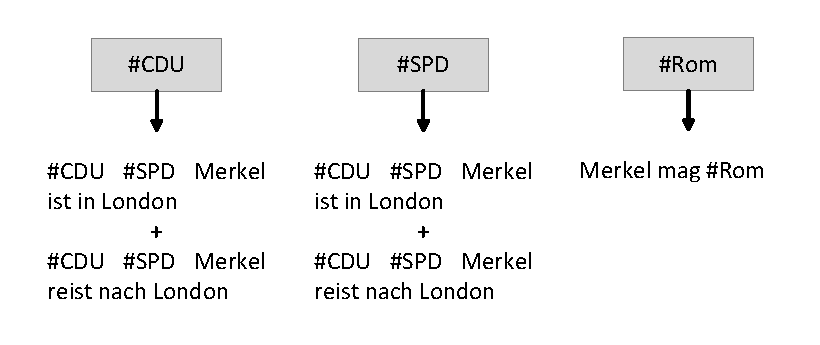
\includegraphics[scale=0.9]{./Bilder/Clustering/HashtagClusteringIdee.pdf}
\caption{Erzeugung eines jeweiligen virtuellen Dokuments zu einem Hashtag}
\label{fig:HashtagClusteringSchritt2}
\end{figure}
%
\item Entferne alle Hashtags, die weniger als $x$ Tweets enthalten. Verschiedene Werte für $x$ wurden ausprobiert und mit $x=15$ gute Ergebnisse erzielt. Dieser Korrekturschritt ist notwendig, damit seltene Hashtags aus der Analyse fallen. Enthält ein Hashtag beispielsweise nur zwei oder drei Tweets, tritt nach wie vor die Problematik der vorherigen Tweet-Analyse auf. Es lassen sich nur wenig aussagekräftige Merkmale ableiten. In Abbildung \ref{fig:HashtagClusteringSchritt2} würde zum Beispiel \glqq \#Rom\grqq{} mit $x=2$ entfernt werden.
%
\item Berechne die Merkmale für jeden Hashtag. Anders als bei der Tweet-Analyse, werden nun die Worthäufigkeiten erfasst.
Während ein Wort bei einem einzelnen Tweet in der Regel nur selten wiederholt wird, kann die Wiederholung bei einem virtuellen Dokument in anderen Größenordnungen auftreten. Daher lohnt es sich hier, als Merkmal die Worthäufigkeit und nicht mehr das bloße Auftreten eines Wortes zu erfassen. Tabelle \ref{fig:ClusterTab3} zeigt die Merkmale für die jeweiligen Hashtags aus dem obigen Beispiel, wobei keine Hashtags entfernt werden.
%
%

\begin{table}[ht]
\centering
\small
\begin{tabular}{cccccccccccc}
\toprule
 & \#CDU & \#SPD  & Merkel & ist & in & London & reist & nach & mag & \#Rom \\ 
\midrule
\#CDU & 2 & 2  & 2 & 1 & 1 & 2 & 1 & 1 & 0 & 0\\ 

\#SPD & 2 & 2  & 2 & 1 & 1 & 2 & 1 & 1 & 0 & 0\\ 

\#Rom & 0 & 0  & 1 & 0 & 0 & 0 & 0 & 0 & 1 & 1\\ 
\bottomrule 
\end{tabular} 
\caption{Quantitative Merkmale eines Hashtags: Worthäufigkeiten}
\label{fig:ClusterTab3}
\end{table}

%
%
\item Dividiere jedes Merkmal eines Hashtags durch die entsprechende Zeilensumme.
Die Zeilensumme stellt die Gesamtanzahl der Wörter eines Hashtags dar. Durch die Division der Häufigkeit eines Wortes durch die Gesamtanzahl ergibt sich ein relativer Anteil dieses Wortes an der Gesamtzahl der verwendeten Wörter. Im Beispiel ergibt sich somit für das Merkmal \glqq Merkel\grqq{} des Hashtags \glqq \#CDU\grqq{} der Wert $2/12$.

Diese Datenvorbereitung ist notwendig, da jedes virtuelle Dokument aus einer anderen Anzahl an Tweets gebildet wird. Ist zum Beispiel das Wort \glqq kerry\grqq{} in 20 von 40 Wörtern beim Hashtag \glqq \#merkel\grqq{} vorhanden und in 10 von 20 Wörtern beim Hashtag \glqq \#steinmeier\grqq{}, so unterscheiden sich beide Hashtags bei der absoluten Wortanzahl deutlich. Relativ gesehen tritt \glqq kerry\grqq{} aber bei beiden Hashtags in 50\% der Wörter auf. Beide Hashtags sind sich also ähnlicher.
%
%
\item Berechne die Distanzmatrix. Da es sich bei der Wortanzahl um ein quantitatives Merkmal handelt, lassen sich nun andere Distanzmaße verwenden. Hier wurde die euklidische Distanz als Metrik eingesetzt. Weitere Scrum-Iterationen sollten auch die Evaluierung anderer Metriken beinhalten. 
%
\item Führe einen Cluster-Algorithmus sowie eine multidimensionale Skalierung durch.
\end{enumerate}
Das beschriebene Vorgehen basiert auf \cite{TsurLittman}, ist aber mit Schritt~3~und~5 sowie mit der multidimensionalen Skalierung aus Schritt~7 entsprechend erweitert. 

In der praktischen Anwendung ergaben sich deutlich bessere Ergebnisse als bei der vorherigen Tweet-Analyse, da die Distanzen auf Grund der mehr zur Verfügung stehenden Informationen aussagekräftiger sind. So wurden zum Beispiel \glqq \#merkel\grqq{}, \glqq \#schumacher\grqq{} und \glqq \#ski\grqq{} (Stand: 12.03.2014, \glqq Alle Sprachen\grqq{}) in einem Cluster dicht aneinander dargestellt. Daraus ließ sich zum Beispiel mit dem News-Modul ableiten, dass viele Tweets den Skiunfall von Merkel und Schumacher behandeln. 

Schwierig ist jedoch die Interpretation im Frontend, warum zwei Hashtags in einem Cluster liegen. Künftige Scrum-Iterationen sollten daher im Frontend zum Beispiel eine Möglichkeit bieten, die Tweets zu zwei markierten Hashtags anzuzeigen. Damit lässt sich besser ein Gefühl vermitteln, wie das Ergebnis zustande gekommen ist.

%Um Hashtags gegenseitig nach ihrer Ähnlichkeit zu bewerten, ist es aber auch alternativ möglich, die \glqq Co-Occurence\grqq{} zwi\-schen zwei Hashtags zu zählen \cite{Antenucci}. Zwei Hashtags sind sich umso ähnlicher, je häufiger sie gemeinsam in einem Tweet auftreten.
%Diese Ähnlichkeitsanalyse ist ebenfalls implementiert worden, wird jedoch aus Laufzeitgründen nicht eingesetzt. 

%Erwin
\subsection{Verwendung der Hashtag-Cluster zur Tweet-Gruppierung} \label{subsec:ClusterTweetsWithHashtags}
Sind die Hashtag-Cluster aus einer Menge an Tweets berechnet, lassen sich nun im wei\-te\-ren Schritt die Tweet-Gruppen berechnen.
Dazu werden die Tweets, die das jeweilige virtuelle Dokument zu einem Hashtag bilden, in den gleichen Cluster eingeordnet wie der entsprechende Hashtag \cite{TsurLittman}. Angenommen, im obigen Beispiel erhält der Hashtag \glqq \#Rom\grqq{} die Cluster-Nummer 2. Alle Tweets, die im virtuellen Dokument von \glqq \#Rom\grqq{} liegen, erhalten somit ebenfalls die Cluster-Nummer 2. 

Ein Problem ist allerdings, dass ein Tweet durchaus in mehreren virtuellen Dokumenten enthalten sein kann, sofern mehrere Hashtags verwendet werden. Besitzen diese unterschiedliche Cluster-Zugehörigkeiten, ist eine 1:1-Zuordnung zwi\-schen Hashtag-Cluster und Tweet-Cluster nicht mehr möglich.

Daher wurde versucht, für jeden Tweet gemäß einer Distanzfunktion den nächsten Hash\-tag zu finden, Der Tweet erbt anschließend die Cluster-Nummer des Hashtags. Damit ist zwar eine eindeutige 1:1-Zuordnung möglich, aber es entsteht erneut das Problem, dass ein Tweet selbst zu wenig Merkmale enthält, um aussagekräftige Distanzen zu den Hashtags abzuleiten. 

Ein wei\-te\-res Problem des Ansatzes ist die Anforderung, 
Tweets durch die multidimensionale Skalierung in die 2D-Ebene 
einzubetten. Ein Tweet selbst erhält nur die 
Cluster-Zugehörigkeit des Hashtags, hat dadurch aber selbst keine Distanzen mehr zu anderen Tweets. 
Alle Tweets würden daher in einem Punkt dargestellt werden, 
dem Punkt, an dem theoretisch der Hashtag liegen würde. 
 Damit lassen sich aber die Distanzen 
zwi\-schen den Tweets nicht mehr interpretieren. Da dies nicht 
die ursprüngliche Motivation widerspiegelt, wurde das Ergebnis 
des hier geschilderten Ansatzes nicht im Frontend dargestellt, 
ist aber nach wie vor implementiert. 


%Wladimir, (Erwin)
\subsection{Cluster-Algorithmen} \label{subsec:ClusterAlgorithmen}

Bei der Wahl der Cluster-Algorithmen haben wir uns auf hierarchische Clusterverfahren 
beschränkt, die ohne Koordinaten der einzelnen Punkte auskommen. 
Der Grund dafür ist, dass man den einzelnen Entitäten, in unserem Fall
Tweets und Hashtags, zunächst keine Positionen zuordnen kann, d.\,h. die Tweets beziehungsweise Hashtags 
haben zwar Ähnlichkeiten zu einander, die man als Distanzen interpretieren kann, aber keine festgelegten 
Positionen in Raum. Es wäre zwar möglich gewesen, zuerst die multidimensionale Skalierung durchzuführen
und anschließend mit Hilfe der gewonnen Positionen zu clustern, aber es ist sehr unwahrscheinlich,
dass eine größere Anzahl an Entitäten mit geringen Fehlern in die 2D-Ebene eingebettet werden können.
Partitionierende Clusteringverfahren, wie $k$-Means \cite{Llo1982} kamen aus diesem Grund nicht in Frage.

Es sind zwei hierarchische Cluster"=Algorithmen implementiert worden, ein Single"=Linkage"=Algorithmus und ein
Complete"=Linkage"=Algorithmus. 
Durch die Implementierung beider Algorithmen ist es möglich, die Auswirkungen beider Ansätze auf das Ergebnis zu beobachten. Da Complete Linkage kompaktere
Cluster erzeugt, haben wir uns für diesen Algorithmus entschieden. Im Folgenden werden die 
beiden Cluster-Algorithmen einzeln vorgestellt.

%Erwin
\subsubsection{Single-Linkage-Algorithmus}
Die Cluster"=Analyse lässt sich auch als Graph-Problem darstellen, wobei die Knoten die zu gruppierenden Objekte darstellen (hier Tweets oder Hashtags). Außerdem handelt es sich um einen vollständigen Graphen, da alle möglichen Objektpaare aus der Distanzmatrix abgebildet werden. Die Kantenkosten sind die jeweiligen Distanzen aus der Distanzmatrix. 

Das Single"=Linkage"=Clustering stellt nun das gleiche Problem 
dar wie die Berechnung des minimalen Spannbaums (MST) durch 
den Kruskal-Algorithmus \cite{Kru1956}. Jede hinzugefügte 
Kante bei der MST-Berechnung stellt einen Fusionierungsschritt 
beim Clustern dar. Sollen beispielsweise $N$ Cluster berechnet 
werden, muss bei der Verwendung einer Union-Find-Datenstruktur 
abgebrochen werden, sobald $N$ Repräsentanten übrig sind.

Der Kruskal"=Algorithmus besitzt eine Laufzeit von $\mathcal{O}(E \log E)$, wobei $E$ die Kantenanzahl darstellt. Da hier ein vollständiger Graph abgearbeitet wird, gilt hier $E = M^2$ mit $M$ als die Anzahl der zu clusternden Entitäten (Knotenanzahl). Durch die Adaption des Kruskal"=Algorithmus besitzt der Single-Linkage-Algorithmus damit eine Laufzeit von $\mathcal{O}(M^2 \log M^2) = \mathcal{O}(M^2 \log M)$.


%Wladimir
\subsubsection{Complete-Linkage-Algorithmus}
Die Idee bei der Implementierung des Complete"=Linkage"=Algorithmus 
war, den naiven hierarchischen Algorithmus zu verwenden, 
an die eigenen Bedürfnisse anzupassen und anschließend die
Laufzeit zu verbessern.

Sei $S=\left\lbrace t_1, \dots, t_M \right\rbrace$ die Menge der zu clusternden Entitäten, 
$d:S^2 \rightarrow \mathbb{R}$ eine Distanzfunktion und $N$ die maximale Anzahl der Cluster,
dann lässt sich der implementierte hierarchische Algorithmus zu Algorithmus \ref{alg:genericHierarchicalAlgorithm}
zusammenfassen.

\begin{algorithm}
 \caption{Generischer hierarchischer Algorithmus}\label{alg:genericHierarchicalAlgorithm}
\begin{algorithmic}[1]
\Statex \textbf{Eingabe:} Menge der Entitäten $\left\lbrace t_1, \dots, t_M\right\rbrace$, $N$ die maximale Anzahl der Cluster
\Statex \textbf{Ausgabe:} Menge der Cluster $\mathcal{C}$
\State $\mathcal{C} = \left\lbrace \left\lbrace t_1 \right\rbrace, \left\lbrace t_2 \right\rbrace, \dots, \left\lbrace t_M \right\rbrace  \right\rbrace$
\For{$(i = 1; i < M\ \textbf{and}\ |\mathcal{C}| > N ; i++)$}
\State $(c_i, c_j) = \operatorname*{arg\,min}\limits_{c_i,c_j \in \mathcal{C},\ i \not= j}  d(c_i, c_j)$
\State $\mathcal{C} = \left( \mathcal{C}\backslash{\left\lbrace c_i,\ c_j \right\rbrace}\right) \cup \left\lbrace c_i \cup c_j \right\rbrace $
\EndFor
\end{algorithmic}
\end{algorithm}

Die Wahl der Funktion $d$ bestimmt das Verhalten des Algorithmus. Wir haben $d$ entsprechend 
dem Complete-Linkage wie folgt gewählt:
\begin{align}
 d(c_i,c_j) := \max{\left\lbrace \delta(t_i,t_j)\ |\ t_i\in c_i, t_j\in c_j \right\rbrace}. \notag
\end{align}
Dabei stellt der Ausdruck $\delta(t_i,t_j)$ die aus der Distanzmatrix stammenden Unähnlichkeiten 
zwi\-schen den Tweets beziehungsweise Hashtags dar.

Bei der naiven Implementierung des obigen Algorithmus beträgt die Laufzeit $\mathcal{O}(M^3)$. Um die Laufzeit auf
$\mathcal{O}(M^2 \log M)$ zu verbessern, haben wir den Algorithmus so mo\-di\-fi\-ziert, dass zur Verwaltung der
Unähnlichkeiten ein Heap verwendet wird. Insgesamt müssen durch den Heap $\frac{M^2}{2}-M \in \mathcal{O}(M^2)$ Werte
verwalten werden. Es werden aber auch maximal $\frac{M^2}{2}-M$ Werte wieder aus dem Heap entfernt, falls $N = 1$ gilt (\textit{worst case}). Insgesamt wird
also zum Erzeugen und Verwalten des Heaps $\mathcal{O}(M^2 + M^2 \log M^2) = \mathcal{O}(M^2 \log M)$ Zeit
benötigt, was auch der Laufzeit von dem implementierten Algorithmus entspricht.

%Wladimir
\subsection{Multidimensionale Skalierung} \label{subsec:MDS}
Das Ziel der multidimensionalen Skalierung ist es, die gegebenen Objekte im Raum oder in der Ebene anzuordnen. 
Dabei sollen die Abstände der Objekte zueinander nach der multidimensionalen Skalierung ihre
Unähnlichkeiten möglichst gut wiedergeben. Dadurch ist es möglich, Objekte, die eigentlich keine Punkte 
im euklidischen Raum sind, als solche zu interpretieren und so Informationen anschaulicher darzustellen oder
neue Zusammenhänge zu entdecken. In der Abbildung \ref{img:MDSAutoMarkenBeispiel} ist die Anwendung
der multidimensionalen Skalierung auf eine Umfrage zu unterschiedlichen Automarken dargestellt. 
Bei der Umfrage haben die Befragten angegeben, wie ähnlich die betroffenen Automarken zueinander sind. Man kann
 sehen, dass bei der geeigneten Wahl von Parametern und Verfahren die Punkte in bestimmten Teilen der Ebene
liegen, die charakteristisch für sie sind, zum Beispiel liegen die Sportwagenhersteller nah bei einander.

\begin{figure}
 \centering
 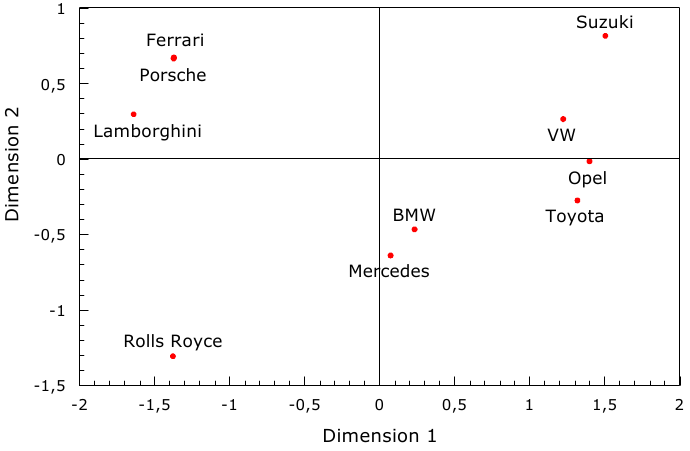
\includegraphics[width=0.8\textwidth]{./Bilder/Clustering/mittlereunaenlichkeitenderautomarken.png}
\caption{Multidimensionale Skalierung angewandt auf eine Umfrage zu Unterschieden 
zwi\-schen bekannten Automarken. Bild entnommen aus \cite{Kappelhoff2001}.}\label{img:MDSAutoMarkenBeispiel}
\end{figure} 

Für unser Projekt haben wir zwei Verfahren zur multidimensionale Skalierung implementiert: \textit{classical scaling} und den Smacof-Algorithmus.
Beide Verfahren sind in \cite{BorgGroenen2005} ausführlich beschrieben. \textit{Classical scaling} ist ein Verfahren, das 
analytisch die multidimensionale Skalierung berechnet, wohingegen der Smacof-Algorithmus ein iteratives Verfahren ist
und wesentlich mehr Parameter bietet. In den folgenden Kapiteln werden die beiden Verfahren kurz vorgestellt. 
Für eine ausführliche Beschreibung der vorgestellten Verfahren verweisen wir auf \cite{BorgGroenen2005}.

%Wladimir
\subsubsection{Classical Scaling}
\textit{Classical scaling} berechnet analytisch zu gegebenen Unähnlichkeiten, die als Distanzen interpretiert werden, eine passende Punktemenge.
Die Abstände der Punkte untereinander entsprechen den gegeben Distanzen, wenn die Dimension des Raumes, in dem die Punkte liegen,
hoch genug ist. 
Der Sinn und Zweck der multidimensionalen Skalierung ist es, die Dimension, in der die Punkte liegen, 
gering zu halten. Damit lassen sich diese grafisch darstellen, wenn die Dimension kleiner als vier ist.
Aus diesem Grund können die berechneten Punkte 
die vorgegebenen Distanzen nur approximieren. Wobei die Approximation schlechter wird, wenn die Anzahl der Dimensionen sinkt.

Sei $\mathbf{\Delta} \in \mathbb{R}^{n\times n}$ die Matrix mit den Distanzen der $n$ Punkte. Ziel ist es eine (von vielen) 
Punktekonstellation zu finden, die diese Matrix erzeugt und eine Approximation davon in einem niedrigdimensionalen Raum zu nehmen.
Das Vorgehen bei \textit{classical scaling} lässt sich dann wie folgt zusammenfassen:
\begin{enumerate}
 \item Berechne $\mathbf{\Delta}^{(2)}=$ Quadrate der Einträge von $\mathbf{\Delta}$.
 \item Berechne $-\tfrac{1}{2}\mathbf{C}_n\mathbf{\Delta}^{(2)}\mathbf{C}_n =: \mathbf{XX}^T$, $\mathbf{C}_n=\mathbf{I}_n-\tfrac{1}{n}\mathbf{1}_n$, 
 $\mathbf{I}_n$ ist die $n$-dimensionale Einheitsmatrix und $\mathbf{1}_n$
 ist die $n$-dimensionale Matrix mit Einsen.
 \item Berechne die Eigenwertdekomposition $\mathbf{XX}^T = \mathbf{Q\Lambda Q}^T = \mathbf{Q\Lambda}^{1/2}(\mathbf{Q\Lambda}^{1/2})^T$, 
 $\mathbf{\Lambda}^{1/2}$ ist Diagonalmatrix mit Quadratwurzeln der Elemente aus $\mathbf{\Lambda}$.
 \item Berechne für ein gewünschtes $d\in \left\lbrace 1,\ 2,\ 3 \right\rbrace$: 
 $\mathbf{X}_d= \mathbf{Q}_d\mathbf{\Lambda}^{1/2}_d$, dabei ist
 $\mathbf{\Lambda}^{1/2}_d$ die Matrix mit den Quadratwurzeln der $d$ größten positiven Eigenwerte und $\mathbf{Q}_d$ ist die Matrix mit 
 entsprechenden Eigenvektoren.
\end{enumerate}

Erklärung der Schritte:
\begin{enumerate}
 \item Nimmt man an, dass man Punkte hat, die die Distanzen aus der Matrix $\mathbf{\Delta}$ erzeugen und die 
 Koordinaten dieser Punkte stehen in der Matrix $\mathbf{X}$ (Zeilenweise),
  dann kann man den quadrierten  euklidische Abstand zweier Vektoren, wie folgt berechnen:
  \begin{align}
   d^2_{ij} = \sum_{k=1}^{n}(x_{ik}-x_{jk})^2 = \sum_{k=1}^{n} (x_{ik}^2 -2x_{ik}x_{jk}+x_{jk}^2). \label{eq:qudeukldist}
  \end{align}
  Berechnet man die quadrierten  euklidischen Abstände für alle Paare, erhält man die Einträge der Matrix $\mathbf{\Delta}^{(2)}$. Man rechnet
  mit den quadrierten Abständen, weil man dadurch die Summe aus \eqref{eq:qudeukldist} in mehrere Summen aufteilen kann. Dadurch kann man die 
  Matrix $\mathbf{\Delta}^{(2)}$ wie folgt schreiben:
  \begin{align*}
   \mathbf{\Delta}^{(2)}(\mathbf{X}) = \mathbf{c}\mathbf{1}^T + \mathbf{1}\mathbf{c}^T - 2\mathbf{X}\mathbf{X}^T,
  \end{align*}
wobei $\mathbf{c}$ ein Vektor mit den Diagonalelementen aus $\mathbf{X}\mathbf{X}^T$ und $\mathbf{1}\in \mathbb{R}^n$ ist ein Vektor mit Einsen sind.
Dieser Zusammenhang ist der Grund für die Berechnung von $\mathbf{\Delta}^{(2)}$.
\item In diesem Schritt wird die Matrix $\mathbf{\Delta}^{(2)}$ beidseitig mit der Matrix $\mathbf{C}_n$ multipliziert ($\mathbf{C}_n$, wie oben in Schritt 2).
Matrix $\mathbf{C}_n$ ist die Zentrierungsmatrix, d.\,h. eine Anwendung auf einen Vektor bewirkt das Subtrahieren des Mittelwertes seiner Einträge von jedem Eintrag, z.\,B.
\begin{align*}
 \mathbf{C}_2 \left( \begin{matrix}
 2 \\
 4 
\end{matrix} \right)
=
\left( \begin{matrix}
 \frac{1}{2} & -\frac{1}{2} \\
 -\frac{1}{2}& \frac{1}{2} 
\end{matrix} \right) \left( \begin{matrix}
 2 \\
 4 
\end{matrix} \right)
=
\left(
\begin{matrix}
 -1 \\
 1 
\end{matrix}
\right).
\end{align*}
Wichtige Spezialfälle sind: 
\begin{itemize}
 \item Zentrierung eines Vektors, der nur Einsen enthält und
 \item Zentrierung  eines bereits zentrierten Vektors.
\end{itemize}
Im ersten Fall erhält man den Nullvektor, weil der Mittelwert eines Vektors nur mit Einsen immer den Wert 1 hat. Im zweiten Fall bewirkt die Zentrierung nichts, da der 
Vektor bereits zentriert ist. Multipliziert man $\mathbf{\Delta}^{(2)}$ beidseitig mit $\mathbf{C}_n$, ergibt sich:
\begin{align*}
 \mathbf{C}_n\mathbf{\Delta}^{(2)}\mathbf{C}_n &= \mathbf{C}_n\left(\mathbf{c}\mathbf{1}^T + \mathbf{1}\mathbf{c}^T - 2\mathbf{X}\mathbf{X^T} \right)\mathbf{C}_n \\
                                               &= \mathbf{C}_n\mathbf{c}\mathbf{1}^T\mathbf{C}_n + \mathbf{C}_n\mathbf{1}\mathbf{c}^T\mathbf{C}_n - 2\mathbf{C}_n\mathbf{X}\mathbf{X^T}\mathbf{C}_n \\
                                               &= \mathbf{C}_n\mathbf{c}\mathbf{0}^T + \mathbf{0}\mathbf{c}^T\mathbf{C}_n - 2\mathbf{C}_n\mathbf{X}\mathbf{X^T}\mathbf{C}_n \\
                                               &=   \underbrace{- 2\mathbf{C}_n\mathbf{X}\mathbf{X^T}\mathbf{C}_n}_{\text{X ist zentriert}} \\
                                               &= -2 \mathbf{X}\mathbf{X^T}.
\end{align*}
Im letzten Schritt der Rechnung nimmt man an, dass die Matrix $\mathbf{X}$ zentriert ist. Das ist keine Einschränkung, weil man eine beliebige Lösung sucht. Außerdem
lässt sich die Lösung durch eine Translation anpassen, sodass die Distanzen zwischen den Punkten unverändert bleiben.

\item Um aus der Matrix $\mathbf{X}\mathbf{X}^T$ die Matrix $\mathbf{X}$ zu extrahieren, benutzt man die Eigenwertdekomposition. Dabei macht man die Annahme, dass 
die Eigenwerte nicht negativ sind.
\item Um eine Approximation von $\mathbf{X}$ für die gewünschte Dimension zu erhalten, benutzt man die größten Eigenwerte und die entsprechenden Eigenvektoren.
\end{enumerate}


Es ist wichtig anzumerken, dass \textit{classical scaling} mit der Hauptkomponentenanalyse
\cite{jolliffe2002principal} eng verwandt ist. Der Unterschied ist hilfreich für das Verständnis des Vorgehens beim \textit{classical scaling}. Bei
der Hauptkomponentenanalyse möchte man die Dimension der betrachteten Punkte reduzieren, während es bei \textit{classical scaling} zusätzlich
darum geht, die Punkte selbst zu finden.

%Wladimir
\subsubsection{Smacof-Algorithmus}
Die Idee beim Smacof-Algorithmus ist, eine gewählte Funktion $\sigma_\mathbf{\Delta}:\mathbb{R}^{n\times d} \rightarrow \mathbb{R}$ zu mi\-ni\-mie\-ren. Die
Funktion $\sigma_\mathbf{\Delta}$ ist dabei ein Maß für den Fehler, der bei der Wahl der $n$ Punkte im $d$-dimensionalen Raum entsteht. Wir haben
in unserer Implementierung $\sigma_\mathbf{\Delta}$ wie folgt gewählt:
\begin{align*}
 \sigma_\mathbf{\Delta}(\mathbf{X}) = \sum_{i=1}^n \sum_{j=i+1}^n (d(\mathbf{x}_i, \mathbf{x}_j) - \delta_{ij})^2.
\end{align*}
Dabei ist $\mathbf{x}_i$ die $i$-te Zeile von $\mathbf{X}$, $d(\mathbf{x}_i, \mathbf{x}_j) = \Vert \mathbf{x}_i^T - \mathbf{x}_j^T  \Vert$,
$\mathbf{\Delta}$ ist die Unähnlichkeitsmatrix (die Einträge an der Position $ij$ geben an, wie unähnlich Entität i zur Entität j ist) und $\delta_{ij}$'s sind die Einträge von $\mathbf{\Delta}$. Die Lösung soll also eine 
Punktmenge sein, sodass die Summe der Quadrate der Differenzen zwischen den resultierenden Abständen und Unähnlichkeiten minimiert wird.

\begin{figure}[ht]
   \centering
   \def\maxW{4.26}
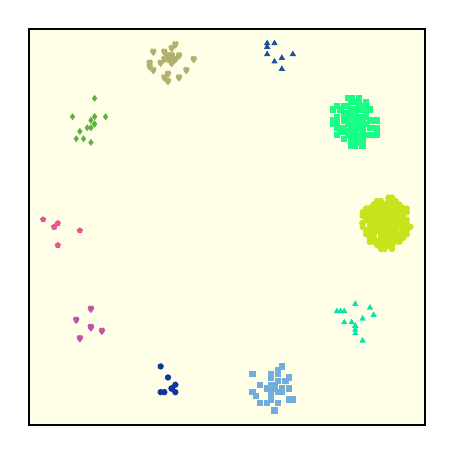
\begin{tikzpicture}[scale=\textwidth/2.6cm, background rectangle/.style={draw=black, thick, fill=yellow!10,},show background rectangle]
\def\marRad{0.2}
\definecolor{color0}{rgb}{0.78,0.89,0.11}
\definecolor{color1}{rgb}{0.10,1.00,0.52}
\definecolor{color2}{rgb}{0.09,0.32,0.64}
\definecolor{color3}{rgb}{0.70,0.69,0.42}
\definecolor{color4}{rgb}{0.36,0.70,0.25}
\definecolor{color5}{rgb}{0.91,0.34,0.56}
\definecolor{color6}{rgb}{0.76,0.33,0.65}
\definecolor{color7}{rgb}{0.06,0.22,0.62}
\definecolor{color8}{rgb}{0.45,0.68,0.87}
\definecolor{color9}{rgb}{0.03,0.89,0.67}
\path[fill=color0,draw=color0,mark size=\marRad, mark=*] plot coordinates {(0.44, -0.03)};
\path[fill=color0,draw=color0,mark size=\marRad, mark=*] plot coordinates {(0.43, 0.01)};
\path[fill=color0,draw=color0,mark size=\marRad, mark=*] plot coordinates {(0.43, -0.05)};
\path[fill=color0,draw=color0,mark size=\marRad, mark=*] plot coordinates {(0.48, 0.00)};
\path[fill=color0,draw=color0,mark size=\marRad, mark=*] plot coordinates {(0.44, -0.01)};
\path[fill=color0,draw=color0,mark size=\marRad, mark=*] plot coordinates {(0.41, 0.00)};
\path[fill=color0,draw=color0,mark size=\marRad, mark=*] plot coordinates {(0.43, -0.01)};
\path[fill=color0,draw=color0,mark size=\marRad, mark=*] plot coordinates {(0.46, -0.00)};
\path[fill=color0,draw=color0,mark size=\marRad, mark=*] plot coordinates {(0.45, -0.00)};
\path[fill=color0,draw=color0,mark size=\marRad, mark=*] plot coordinates {(0.41, -0.02)};
\path[fill=color0,draw=color0,mark size=\marRad, mark=*] plot coordinates {(0.47, 0.03)};
\path[fill=color0,draw=color0,mark size=\marRad, mark=*] plot coordinates {(0.46, -0.00)};
\path[fill=color0,draw=color0,mark size=\marRad, mark=*] plot coordinates {(0.42, 0.02)};
\path[fill=color0,draw=color0,mark size=\marRad, mark=*] plot coordinates {(0.38, -0.00)};
\path[fill=color0,draw=color0,mark size=\marRad, mark=*] plot coordinates {(0.41, -0.00)};
\path[fill=color0,draw=color0,mark size=\marRad, mark=*] plot coordinates {(0.43, 0.01)};
\path[fill=color0,draw=color0,mark size=\marRad, mark=*] plot coordinates {(0.43, -0.06)};
\path[fill=color0,draw=color0,mark size=\marRad, mark=*] plot coordinates {(0.45, 0.01)};
\path[fill=color0,draw=color0,mark size=\marRad, mark=*] plot coordinates {(0.40, -0.03)};
\path[fill=color0,draw=color0,mark size=\marRad, mark=*] plot coordinates {(0.44, -0.01)};
\path[fill=color0,draw=color0,mark size=\marRad, mark=*] plot coordinates {(0.45, 0.07)};
\path[fill=color0,draw=color0,mark size=\marRad, mark=*] plot coordinates {(0.46, -0.05)};
\path[fill=color0,draw=color0,mark size=\marRad, mark=*] plot coordinates {(0.46, 0.04)};
\path[fill=color0,draw=color0,mark size=\marRad, mark=*] plot coordinates {(0.38, -0.00)};
\path[fill=color0,draw=color0,mark size=\marRad, mark=*] plot coordinates {(0.47, 0.04)};
\path[fill=color0,draw=color0,mark size=\marRad, mark=*] plot coordinates {(0.45, -0.01)};
\path[fill=color0,draw=color0,mark size=\marRad, mark=*] plot coordinates {(0.42, -0.02)};
\path[fill=color0,draw=color0,mark size=\marRad, mark=*] plot coordinates {(0.42, 0.03)};
\path[fill=color0,draw=color0,mark size=\marRad, mark=*] plot coordinates {(0.43, 0.06)};
\path[fill=color0,draw=color0,mark size=\marRad, mark=*] plot coordinates {(0.44, -0.06)};
\path[fill=color0,draw=color0,mark size=\marRad, mark=*] plot coordinates {(0.47, 0.01)};
\path[fill=color0,draw=color0,mark size=\marRad, mark=*] plot coordinates {(0.48, -0.05)};
\path[fill=color0,draw=color0,mark size=\marRad, mark=*] plot coordinates {(0.49, 0.02)};
\path[fill=color0,draw=color0,mark size=\marRad, mark=*] plot coordinates {(0.46, -0.01)};
\path[fill=color0,draw=color0,mark size=\marRad, mark=*] plot coordinates {(0.42, 0.04)};
\path[fill=color0,draw=color0,mark size=\marRad, mark=*] plot coordinates {(0.44, 0.00)};
\path[fill=color0,draw=color0,mark size=\marRad, mark=*] plot coordinates {(0.42, 0.01)};
\path[fill=color0,draw=color0,mark size=\marRad, mark=*] plot coordinates {(0.41, -0.02)};
\path[fill=color0,draw=color0,mark size=\marRad, mark=*] plot coordinates {(0.48, 0.03)};
\path[fill=color0,draw=color0,mark size=\marRad, mark=*] plot coordinates {(0.42, 0.06)};
\path[fill=color0,draw=color0,mark size=\marRad, mark=*] plot coordinates {(0.40, -0.05)};
\path[fill=color0,draw=color0,mark size=\marRad, mark=*] plot coordinates {(0.41, 0.04)};
\path[fill=color0,draw=color0,mark size=\marRad, mark=*] plot coordinates {(0.44, -0.03)};
\path[fill=color0,draw=color0,mark size=\marRad, mark=*] plot coordinates {(0.45, -0.02)};
\path[fill=color0,draw=color0,mark size=\marRad, mark=*] plot coordinates {(0.41, -0.00)};
\path[fill=color0,draw=color0,mark size=\marRad, mark=*] plot coordinates {(0.44, 0.00)};
\path[fill=color0,draw=color0,mark size=\marRad, mark=*] plot coordinates {(0.40, 0.02)};
\path[fill=color0,draw=color0,mark size=\marRad, mark=*] plot coordinates {(0.43, 0.05)};
\path[fill=color0,draw=color0,mark size=\marRad, mark=*] plot coordinates {(0.51, -0.01)};
\path[fill=color0,draw=color0,mark size=\marRad, mark=*] plot coordinates {(0.46, 0.03)};
\path[fill=color0,draw=color0,mark size=\marRad, mark=*] plot coordinates {(0.43, -0.02)};
\path[fill=color0,draw=color0,mark size=\marRad, mark=*] plot coordinates {(0.50, 0.03)};
\path[fill=color0,draw=color0,mark size=\marRad, mark=*] plot coordinates {(0.44, 0.02)};
\path[fill=color0,draw=color0,mark size=\marRad, mark=*] plot coordinates {(0.48, -0.04)};
\path[fill=color0,draw=color0,mark size=\marRad, mark=*] plot coordinates {(0.43, 0.01)};
\path[fill=color0,draw=color0,mark size=\marRad, mark=*] plot coordinates {(0.49, 0.01)};
\path[fill=color0,draw=color0,mark size=\marRad, mark=*] plot coordinates {(0.44, -0.02)};
\path[fill=color0,draw=color0,mark size=\marRad, mark=*] plot coordinates {(0.43, 0.01)};
\path[fill=color0,draw=color0,mark size=\marRad, mark=*] plot coordinates {(0.46, -0.03)};
\path[fill=color0,draw=color0,mark size=\marRad, mark=*] plot coordinates {(0.44, 0.00)};
\path[fill=color0,draw=color0,mark size=\marRad, mark=*] plot coordinates {(0.42, -0.01)};
\path[fill=color0,draw=color0,mark size=\marRad, mark=*] plot coordinates {(0.49, -0.02)};
\path[fill=color0,draw=color0,mark size=\marRad, mark=*] plot coordinates {(0.44, -0.00)};
\path[fill=color0,draw=color0,mark size=\marRad, mark=*] plot coordinates {(0.45, -0.01)};
\path[fill=color0,draw=color0,mark size=\marRad, mark=*] plot coordinates {(0.50, 0.04)};
\path[fill=color0,draw=color0,mark size=\marRad, mark=*] plot coordinates {(0.44, 0.00)};
\path[fill=color0,draw=color0,mark size=\marRad, mark=*] plot coordinates {(0.45, 0.00)};
\path[fill=color0,draw=color0,mark size=\marRad, mark=*] plot coordinates {(0.39, 0.01)};
\path[fill=color0,draw=color0,mark size=\marRad, mark=*] plot coordinates {(0.47, -0.00)};
\path[fill=color0,draw=color0,mark size=\marRad, mark=*] plot coordinates {(0.45, -0.01)};
\path[fill=color0,draw=color0,mark size=\marRad, mark=*] plot coordinates {(0.44, 0.01)};
\path[fill=color0,draw=color0,mark size=\marRad, mark=*] plot coordinates {(0.44, -0.01)};
\path[fill=color0,draw=color0,mark size=\marRad, mark=*] plot coordinates {(0.45, -0.00)};
\path[fill=color0,draw=color0,mark size=\marRad, mark=*] plot coordinates {(0.46, 0.06)};
\path[fill=color0,draw=color0,mark size=\marRad, mark=*] plot coordinates {(0.44, 0.04)};
\path[fill=color0,draw=color0,mark size=\marRad, mark=*] plot coordinates {(0.40, -0.00)};
\path[fill=color0,draw=color0,mark size=\marRad, mark=*] plot coordinates {(0.48, 0.01)};
\path[fill=color0,draw=color0,mark size=\marRad, mark=*] plot coordinates {(0.40, 0.04)};
\path[fill=color0,draw=color0,mark size=\marRad, mark=*] plot coordinates {(0.45, -0.00)};
\path[fill=color0,draw=color0,mark size=\marRad, mark=*] plot coordinates {(0.46, 0.01)};
\path[fill=color0,draw=color0,mark size=\marRad, mark=*] plot coordinates {(0.45, 0.04)};
\path[fill=color0,draw=color0,mark size=\marRad, mark=*] plot coordinates {(0.43, 0.06)};
\path[fill=color0,draw=color0,mark size=\marRad, mark=*] plot coordinates {(0.40, -0.01)};
\path[fill=color0,draw=color0,mark size=\marRad, mark=*] plot coordinates {(0.45, 0.02)};
\path[fill=color0,draw=color0,mark size=\marRad, mark=*] plot coordinates {(0.46, 0.00)};
\path[fill=color0,draw=color0,mark size=\marRad, mark=*] plot coordinates {(0.47, 0.02)};
\path[fill=color0,draw=color0,mark size=\marRad, mark=*] plot coordinates {(0.45, 0.00)};
\path[fill=color0,draw=color0,mark size=\marRad, mark=*] plot coordinates {(0.49, -0.04)};
\path[fill=color0,draw=color0,mark size=\marRad, mark=*] plot coordinates {(0.45, -0.02)};
\path[fill=color0,draw=color0,mark size=\marRad, mark=*] plot coordinates {(0.48, 0.04)};
\path[fill=color0,draw=color0,mark size=\marRad, mark=*] plot coordinates {(0.44, 0.00)};
\path[fill=color0,draw=color0,mark size=\marRad, mark=*] plot coordinates {(0.44, 0.01)};
\path[fill=color0,draw=color0,mark size=\marRad, mark=*] plot coordinates {(0.46, 0.02)};
\path[fill=color0,draw=color0,mark size=\marRad, mark=*] plot coordinates {(0.40, -0.01)};
\path[fill=color0,draw=color0,mark size=\marRad, mark=*] plot coordinates {(0.45, 0.01)};
\path[fill=color0,draw=color0,mark size=\marRad, mark=*] plot coordinates {(0.44, -0.00)};
\path[fill=color0,draw=color0,mark size=\marRad, mark=*] plot coordinates {(0.43, -0.01)};
\path[fill=color0,draw=color0,mark size=\marRad, mark=*] plot coordinates {(0.49, 0.03)};
\path[fill=color0,draw=color0,mark size=\marRad, mark=*] plot coordinates {(0.42, 0.03)};
\path[fill=color0,draw=color0,mark size=\marRad, mark=*] plot coordinates {(0.48, -0.03)};
\path[fill=color0,draw=color0,mark size=\marRad, mark=*] plot coordinates {(0.44, -0.00)};
\path[fill=color0,draw=color0,mark size=\marRad, mark=*] plot coordinates {(0.45, 0.01)};
\path[fill=color0,draw=color0,mark size=\marRad, mark=*] plot coordinates {(0.44, -0.06)};
\path[fill=color0,draw=color0,mark size=\marRad, mark=*] plot coordinates {(0.42, 0.02)};
\path[fill=color0,draw=color0,mark size=\marRad, mark=*] plot coordinates {(0.44, -0.04)};
\path[fill=color0,draw=color0,mark size=\marRad, mark=*] plot coordinates {(0.49, -0.01)};
\path[fill=color0,draw=color0,mark size=\marRad, mark=*] plot coordinates {(0.43, -0.00)};
\path[fill=color0,draw=color0,mark size=\marRad, mark=*] plot coordinates {(0.44, -0.05)};
\path[fill=color0,draw=color0,mark size=\marRad, mark=*] plot coordinates {(0.47, 0.01)};
\path[fill=color0,draw=color0,mark size=\marRad, mark=*] plot coordinates {(0.46, -0.03)};
\path[fill=color0,draw=color0,mark size=\marRad, mark=*] plot coordinates {(0.41, -0.04)};
\path[fill=color0,draw=color0,mark size=\marRad, mark=*] plot coordinates {(0.41, 0.05)};
\path[fill=color0,draw=color0,mark size=\marRad, mark=*] plot coordinates {(0.42, -0.05)};
\path[fill=color0,draw=color0,mark size=\marRad, mark=*] plot coordinates {(0.48, -0.04)};
\path[fill=color0,draw=color0,mark size=\marRad, mark=*] plot coordinates {(0.42, -0.00)};
\path[fill=color0,draw=color0,mark size=\marRad, mark=*] plot coordinates {(0.46, 0.00)};
\path[fill=color0,draw=color0,mark size=\marRad, mark=*] plot coordinates {(0.44, 0.01)};
\path[fill=color0,draw=color0,mark size=\marRad, mark=*] plot coordinates {(0.43, 0.04)};
\path[fill=color0,draw=color0,mark size=\marRad, mark=*] plot coordinates {(0.45, 0.03)};
\path[fill=color0,draw=color0,mark size=\marRad, mark=*] plot coordinates {(0.47, 0.02)};
\path[fill=color0,draw=color0,mark size=\marRad, mark=*] plot coordinates {(0.46, -0.06)};
\path[fill=color0,draw=color0,mark size=\marRad, mark=*] plot coordinates {(0.46, -0.01)};
\path[fill=color0,draw=color0,mark size=\marRad, mark=*] plot coordinates {(0.43, 0.03)};
\path[fill=color0,draw=color0,mark size=\marRad, mark=*] plot coordinates {(0.46, -0.03)};
\path[fill=color0,draw=color0,mark size=\marRad, mark=*] plot coordinates {(0.43, 0.05)};
\path[fill=color0,draw=color0,mark size=\marRad, mark=*] plot coordinates {(0.46, 0.04)};
\path[fill=color0,draw=color0,mark size=\marRad, mark=*] plot coordinates {(0.46, 0.04)};
\path[fill=color0,draw=color0,mark size=\marRad, mark=*] plot coordinates {(0.39, 0.01)};
\path[fill=color0,draw=color0,mark size=\marRad, mark=*] plot coordinates {(0.46, -0.03)};
\path[fill=color0,draw=color0,mark size=\marRad, mark=*] plot coordinates {(0.46, 0.02)};
\path[fill=color0,draw=color0,mark size=\marRad, mark=*] plot coordinates {(0.45, 0.00)};
\path[fill=color0,draw=color0,mark size=\marRad, mark=*] plot coordinates {(0.48, -0.03)};
\path[fill=color0,draw=color0,mark size=\marRad, mark=*] plot coordinates {(0.45, 0.03)};
\path[fill=color0,draw=color0,mark size=\marRad, mark=*] plot coordinates {(0.43, -0.01)};
\path[fill=color0,draw=color0,mark size=\marRad, mark=*] plot coordinates {(0.45, 0.00)};
\path[fill=color0,draw=color0,mark size=\marRad, mark=*] plot coordinates {(0.44, -0.05)};
\path[fill=color0,draw=color0,mark size=\marRad, mark=*] plot coordinates {(0.45, 0.01)};
\path[fill=color0,draw=color0,mark size=\marRad, mark=*] plot coordinates {(0.44, -0.01)};
\path[fill=color0,draw=color0,mark size=\marRad, mark=*] plot coordinates {(0.45, 0.02)};
\path[fill=color0,draw=color0,mark size=\marRad, mark=*] plot coordinates {(0.46, 0.01)};
\path[fill=color0,draw=color0,mark size=\marRad, mark=*] plot coordinates {(0.44, -0.01)};
\path[fill=color0,draw=color0,mark size=\marRad, mark=*] plot coordinates {(0.48, 0.01)};
\path[fill=color0,draw=color0,mark size=\marRad, mark=*] plot coordinates {(0.42, 0.01)};
\path[fill=color0,draw=color0,mark size=\marRad, mark=*] plot coordinates {(0.49, 0.03)};
\path[fill=color0,draw=color0,mark size=\marRad, mark=*] plot coordinates {(0.39, -0.02)};
\path[fill=color0,draw=color0,mark size=\marRad, mark=*] plot coordinates {(0.46, -0.05)};
\path[fill=color0,draw=color0,mark size=\marRad, mark=*] plot coordinates {(0.45, -0.06)};
\path[fill=color0,draw=color0,mark size=\marRad, mark=*] plot coordinates {(0.40, -0.03)};
\path[fill=color0,draw=color0,mark size=\marRad, mark=*] plot coordinates {(0.44, -0.07)};
\path[fill=color0,draw=color0,mark size=\marRad, mark=*] plot coordinates {(0.49, 0.03)};
\path[fill=color0,draw=color0,mark size=\marRad, mark=*] plot coordinates {(0.45, -0.05)};
\path[fill=color0,draw=color0,mark size=\marRad, mark=*] plot coordinates {(0.44, -0.01)};
\path[fill=color0,draw=color0,mark size=\marRad, mark=*] plot coordinates {(0.48, 0.02)};
\path[fill=color0,draw=color0,mark size=\marRad, mark=*] plot coordinates {(0.45, 0.05)};
\path[fill=color0,draw=color0,mark size=\marRad, mark=*] plot coordinates {(0.47, 0.03)};
\path[fill=color0,draw=color0,mark size=\marRad, mark=*] plot coordinates {(0.42, 0.06)};
\path[fill=color0,draw=color0,mark size=\marRad, mark=*] plot coordinates {(0.48, 0.01)};
\path[fill=color0,draw=color0,mark size=\marRad, mark=*] plot coordinates {(0.47, -0.02)};
\path[fill=color0,draw=color0,mark size=\marRad, mark=*] plot coordinates {(0.43, -0.00)};
\path[fill=color0,draw=color0,mark size=\marRad, mark=*] plot coordinates {(0.46, 0.00)};
\path[fill=color0,draw=color0,mark size=\marRad, mark=*] plot coordinates {(0.45, -0.03)};
\path[fill=color0,draw=color0,mark size=\marRad, mark=*] plot coordinates {(0.43, 0.02)};
\path[fill=color0,draw=color0,mark size=\marRad, mark=*] plot coordinates {(0.43, -0.06)};
\path[fill=color0,draw=color0,mark size=\marRad, mark=*] plot coordinates {(0.46, -0.01)};
\path[fill=color0,draw=color0,mark size=\marRad, mark=*] plot coordinates {(0.45, 0.03)};
\path[fill=color0,draw=color0,mark size=\marRad, mark=*] plot coordinates {(0.46, 0.05)};
\path[fill=color0,draw=color0,mark size=\marRad, mark=*] plot coordinates {(0.46, 0.03)};
\path[fill=color0,draw=color0,mark size=\marRad, mark=*] plot coordinates {(0.47, 0.01)};
\path[fill=color0,draw=color0,mark size=\marRad, mark=*] plot coordinates {(0.44, -0.00)};
\path[fill=color0,draw=color0,mark size=\marRad, mark=*] plot coordinates {(0.44, 0.01)};
\path[fill=color0,draw=color0,mark size=\marRad, mark=*] plot coordinates {(0.41, -0.04)};
\path[fill=color0,draw=color0,mark size=\marRad, mark=*] plot coordinates {(0.44, 0.02)};
\path[fill=color0,draw=color0,mark size=\marRad, mark=*] plot coordinates {(0.45, -0.03)};
\path[fill=color0,draw=color0,mark size=\marRad, mark=*] plot coordinates {(0.47, 0.02)};
\path[fill=color0,draw=color0,mark size=\marRad, mark=*] plot coordinates {(0.48, -0.01)};
\path[fill=color0,draw=color0,mark size=\marRad, mark=*] plot coordinates {(0.47, 0.02)};
\path[fill=color0,draw=color0,mark size=\marRad, mark=*] plot coordinates {(0.47, -0.00)};
\path[fill=color0,draw=color0,mark size=\marRad, mark=*] plot coordinates {(0.45, 0.04)};
\path[fill=color0,draw=color0,mark size=\marRad, mark=*] plot coordinates {(0.41, -0.03)};
\path[fill=color0,draw=color0,mark size=\marRad, mark=*] plot coordinates {(0.44, 0.00)};
\path[fill=color0,draw=color0,mark size=\marRad, mark=*] plot coordinates {(0.47, -0.03)};
\path[fill=color0,draw=color0,mark size=\marRad, mark=*] plot coordinates {(0.46, 0.01)};
\path[fill=color0,draw=color0,mark size=\marRad, mark=*] plot coordinates {(0.44, -0.01)};
\path[fill=color0,draw=color0,mark size=\marRad, mark=*] plot coordinates {(0.50, 0.00)};
\path[fill=color0,draw=color0,mark size=\marRad, mark=*] plot coordinates {(0.45, -0.00)};
\path[fill=color0,draw=color0,mark size=\marRad, mark=*] plot coordinates {(0.45, -0.03)};
\path[fill=color0,draw=color0,mark size=\marRad, mark=*] plot coordinates {(0.41, -0.05)};
\path[fill=color0,draw=color0,mark size=\marRad, mark=*] plot coordinates {(0.48, -0.05)};
\path[fill=color0,draw=color0,mark size=\marRad, mark=*] plot coordinates {(0.50, -0.02)};
\path[fill=color0,draw=color0,mark size=\marRad, mark=*] plot coordinates {(0.42, -0.02)};
\path[fill=color0,draw=color0,mark size=\marRad, mark=*] plot coordinates {(0.43, 0.05)};
\path[fill=color0,draw=color0,mark size=\marRad, mark=*] plot coordinates {(0.44, 0.02)};
\path[fill=color0,draw=color0,mark size=\marRad, mark=*] plot coordinates {(0.45, -0.05)};
\path[fill=color0,draw=color0,mark size=\marRad, mark=*] plot coordinates {(0.45, -0.05)};
\path[fill=color0,draw=color0,mark size=\marRad, mark=*] plot coordinates {(0.44, 0.00)};
\path[fill=color0,draw=color0,mark size=\marRad, mark=*] plot coordinates {(0.45, -0.04)};
\path[fill=color0,draw=color0,mark size=\marRad, mark=*] plot coordinates {(0.40, 0.04)};
\path[fill=color0,draw=color0,mark size=\marRad, mark=*] plot coordinates {(0.38, 0.03)};
\path[fill=color0,draw=color0,mark size=\marRad, mark=*] plot coordinates {(0.49, 0.00)};
\path[fill=color0,draw=color0,mark size=\marRad, mark=*] plot coordinates {(0.48, -0.05)};
\path[fill=color0,draw=color0,mark size=\marRad, mark=*] plot coordinates {(0.45, 0.02)};
\path[fill=color0,draw=color0,mark size=\marRad, mark=*] plot coordinates {(0.41, 0.00)};
\path[fill=color0,draw=color0,mark size=\marRad, mark=*] plot coordinates {(0.42, -0.05)};
\path[fill=color0,draw=color0,mark size=\marRad, mark=*] plot coordinates {(0.45, -0.05)};
\path[fill=color0,draw=color0,mark size=\marRad, mark=*] plot coordinates {(0.43, -0.05)};
\path[fill=color0,draw=color0,mark size=\marRad, mark=*] plot coordinates {(0.42, -0.06)};
\path[fill=color0,draw=color0,mark size=\marRad, mark=*] plot coordinates {(0.48, 0.04)};
\path[fill=color0,draw=color0,mark size=\marRad, mark=*] plot coordinates {(0.44, -0.00)};
\path[fill=color0,draw=color0,mark size=\marRad, mark=*] plot coordinates {(0.39, 0.02)};
\path[fill=color0,draw=color0,mark size=\marRad, mark=*] plot coordinates {(0.40, -0.05)};
\path[fill=color0,draw=color0,mark size=\marRad, mark=*] plot coordinates {(0.44, 0.01)};
\path[fill=color0,draw=color0,mark size=\marRad, mark=*] plot coordinates {(0.44, 0.00)};
\path[fill=color0,draw=color0,mark size=\marRad, mark=*] plot coordinates {(0.46, -0.05)};
\path[fill=color0,draw=color0,mark size=\marRad, mark=*] plot coordinates {(0.47, 0.06)};
\path[fill=color0,draw=color0,mark size=\marRad, mark=*] plot coordinates {(0.41, 0.05)};
\path[fill=color0,draw=color0,mark size=\marRad, mark=*] plot coordinates {(0.43, -0.05)};
\path[fill=color0,draw=color0,mark size=\marRad, mark=*] plot coordinates {(0.41, -0.01)};
\path[fill=color0,draw=color0,mark size=\marRad, mark=*] plot coordinates {(0.45, -0.01)};
\path[fill=color0,draw=color0,mark size=\marRad, mark=*] plot coordinates {(0.44, -0.03)};
\path[fill=color0,draw=color0,mark size=\marRad, mark=*] plot coordinates {(0.48, 0.05)};
\path[fill=color0,draw=color0,mark size=\marRad, mark=*] plot coordinates {(0.44, 0.00)};
\path[fill=color0,draw=color0,mark size=\marRad, mark=*] plot coordinates {(0.43, -0.05)};
\path[fill=color0,draw=color0,mark size=\marRad, mark=*] plot coordinates {(0.40, -0.05)};
\path[fill=color0,draw=color0,mark size=\marRad, mark=*] plot coordinates {(0.50, 0.03)};
\path[fill=color0,draw=color0,mark size=\marRad, mark=*] plot coordinates {(0.41, 0.00)};
\path[fill=color0,draw=color0,mark size=\marRad, mark=*] plot coordinates {(0.49, -0.03)};
\path[fill=color0,draw=color0,mark size=\marRad, mark=*] plot coordinates {(0.39, 0.04)};
\path[fill=color0,draw=color0,mark size=\marRad, mark=*] plot coordinates {(0.44, -0.02)};
\path[fill=color0,draw=color0,mark size=\marRad, mark=*] plot coordinates {(0.44, 0.04)};
\path[fill=color0,draw=color0,mark size=\marRad, mark=*] plot coordinates {(0.44, 0.00)};
\path[fill=color0,draw=color0,mark size=\marRad, mark=*] plot coordinates {(0.40, 0.04)};
\path[fill=color0,draw=color0,mark size=\marRad, mark=*] plot coordinates {(0.40, 0.01)};
\path[fill=color0,draw=color0,mark size=\marRad, mark=*] plot coordinates {(0.50, -0.01)};
\path[fill=color0,draw=color0,mark size=\marRad, mark=*] plot coordinates {(0.39, -0.03)};
\path[fill=color0,draw=color0,mark size=\marRad, mark=*] plot coordinates {(0.44, 0.03)};
\path[fill=color0,draw=color0,mark size=\marRad, mark=*] plot coordinates {(0.47, -0.02)};
\path[fill=color0,draw=color0,mark size=\marRad, mark=*] plot coordinates {(0.41, 0.01)};
\path[fill=color0,draw=color0,mark size=\marRad, mark=*] plot coordinates {(0.47, -0.04)};
\path[fill=color0,draw=color0,mark size=\marRad, mark=*] plot coordinates {(0.46, -0.01)};
\path[fill=color0,draw=color0,mark size=\marRad, mark=*] plot coordinates {(0.45, 0.00)};
\path[fill=color0,draw=color0,mark size=\marRad, mark=*] plot coordinates {(0.45, 0.01)};
\path[fill=color0,draw=color0,mark size=\marRad, mark=*] plot coordinates {(0.46, -0.04)};
\path[fill=color0,draw=color0,mark size=\marRad, mark=*] plot coordinates {(0.46, 0.01)};
\path[fill=color0,draw=color0,mark size=\marRad, mark=*] plot coordinates {(0.46, -0.01)};
\path[fill=color0,draw=color0,mark size=\marRad, mark=*] plot coordinates {(0.43, 0.02)};
\path[fill=color0,draw=color0,mark size=\marRad, mark=*] plot coordinates {(0.39, 0.03)};
\path[fill=color0,draw=color0,mark size=\marRad, mark=*] plot coordinates {(0.41, -0.03)};
\path[fill=color0,draw=color0,mark size=\marRad, mark=*] plot coordinates {(0.46, 0.01)};
\path[fill=color0,draw=color0,mark size=\marRad, mark=*] plot coordinates {(0.48, 0.04)};
\path[fill=color0,draw=color0,mark size=\marRad, mark=*] plot coordinates {(0.43, -0.03)};
\path[fill=color0,draw=color0,mark size=\marRad, mark=*] plot coordinates {(0.44, -0.01)};
\path[fill=color0,draw=color0,mark size=\marRad, mark=*] plot coordinates {(0.50, -0.03)};
\path[fill=color0,draw=color0,mark size=\marRad, mark=*] plot coordinates {(0.44, 0.03)};
\path[fill=color0,draw=color0,mark size=\marRad, mark=*] plot coordinates {(0.46, -0.02)};
\path[fill=color0,draw=color0,mark size=\marRad, mark=*] plot coordinates {(0.44, 0.01)};
\path[fill=color0,draw=color0,mark size=\marRad, mark=*] plot coordinates {(0.43, 0.01)};
\path[fill=color0,draw=color0,mark size=\marRad, mark=*] plot coordinates {(0.49, 0.04)};
\path[fill=color0,draw=color0,mark size=\marRad, mark=*] plot coordinates {(0.44, 0.02)};
\path[fill=color0,draw=color0,mark size=\marRad, mark=*] plot coordinates {(0.45, -0.00)};
\path[fill=color0,draw=color0,mark size=\marRad, mark=*] plot coordinates {(0.45, -0.00)};
\path[fill=color0,draw=color0,mark size=\marRad, mark=*] plot coordinates {(0.45, 0.01)};
\path[fill=color0,draw=color0,mark size=\marRad, mark=*] plot coordinates {(0.48, 0.04)};
\path[fill=color0,draw=color0,mark size=\marRad, mark=*] plot coordinates {(0.44, -0.01)};
\path[fill=color0,draw=color0,mark size=\marRad, mark=*] plot coordinates {(0.38, 0.00)};
\path[fill=color0,draw=color0,mark size=\marRad, mark=*] plot coordinates {(0.43, -0.02)};
\path[fill=color0,draw=color0,mark size=\marRad, mark=*] plot coordinates {(0.44, -0.03)};
\path[fill=color0,draw=color0,mark size=\marRad, mark=*] plot coordinates {(0.41, -0.02)};
\path[fill=color0,draw=color0,mark size=\marRad, mark=*] plot coordinates {(0.40, -0.04)};
\path[fill=color0,draw=color0,mark size=\marRad, mark=*] plot coordinates {(0.44, 0.00)};
\path[fill=color0,draw=color0,mark size=\marRad, mark=*] plot coordinates {(0.39, 0.01)};
\path[fill=color0,draw=color0,mark size=\marRad, mark=*] plot coordinates {(0.47, 0.03)};
\path[fill=color0,draw=color0,mark size=\marRad, mark=*] plot coordinates {(0.44, 0.00)};
\path[fill=color0,draw=color0,mark size=\marRad, mark=*] plot coordinates {(0.48, 0.04)};
\path[fill=color0,draw=color0,mark size=\marRad, mark=*] plot coordinates {(0.47, 0.04)};
\path[fill=color0,draw=color0,mark size=\marRad, mark=*] plot coordinates {(0.38, 0.02)};
\path[fill=color0,draw=color0,mark size=\marRad, mark=*] plot coordinates {(0.43, -0.00)};
\path[fill=color0,draw=color0,mark size=\marRad, mark=*] plot coordinates {(0.40, 0.01)};
\path[fill=color0,draw=color0,mark size=\marRad, mark=*] plot coordinates {(0.41, 0.01)};
\path[fill=color0,draw=color0,mark size=\marRad, mark=*] plot coordinates {(0.44, -0.01)};
\path[fill=color0,draw=color0,mark size=\marRad, mark=*] plot coordinates {(0.45, 0.03)};
\path[fill=color0,draw=color0,mark size=\marRad, mark=*] plot coordinates {(0.43, -0.05)};
\path[fill=color0,draw=color0,mark size=\marRad, mark=*] plot coordinates {(0.45, -0.02)};
\path[fill=color0,draw=color0,mark size=\marRad, mark=*] plot coordinates {(0.44, -0.00)};
\path[fill=color0,draw=color0,mark size=\marRad, mark=*] plot coordinates {(0.50, 0.03)};
\path[fill=color0,draw=color0,mark size=\marRad, mark=*] plot coordinates {(0.42, 0.06)};
\path[fill=color0,draw=color0,mark size=\marRad, mark=*] plot coordinates {(0.44, -0.00)};
\path[fill=color0,draw=color0,mark size=\marRad, mark=*] plot coordinates {(0.43, -0.03)};
\path[fill=color0,draw=color0,mark size=\marRad, mark=*] plot coordinates {(0.43, 0.05)};
\path[fill=color0,draw=color0,mark size=\marRad, mark=*] plot coordinates {(0.47, -0.04)};
\path[fill=color0,draw=color0,mark size=\marRad, mark=*] plot coordinates {(0.44, -0.00)};
\path[fill=color0,draw=color0,mark size=\marRad, mark=*] plot coordinates {(0.39, 0.04)};
\path[fill=color0,draw=color0,mark size=\marRad, mark=*] plot coordinates {(0.49, 0.04)};
\path[fill=color0,draw=color0,mark size=\marRad, mark=*] plot coordinates {(0.45, 0.00)};
\path[fill=color0,draw=color0,mark size=\marRad, mark=*] plot coordinates {(0.40, 0.02)};
\path[fill=color0,draw=color0,mark size=\marRad, mark=*] plot coordinates {(0.38, -0.00)};
\path[fill=color0,draw=color0,mark size=\marRad, mark=*] plot coordinates {(0.44, -0.01)};
\path[fill=color0,draw=color0,mark size=\marRad, mark=*] plot coordinates {(0.44, -0.06)};
\path[fill=color0,draw=color0,mark size=\marRad, mark=*] plot coordinates {(0.40, -0.05)};
\path[fill=color0,draw=color0,mark size=\marRad, mark=*] plot coordinates {(0.50, -0.02)};
\path[fill=color0,draw=color0,mark size=\marRad, mark=*] plot coordinates {(0.44, 0.03)};
\path[fill=color0,draw=color0,mark size=\marRad, mark=*] plot coordinates {(0.45, 0.02)};
\path[fill=color0,draw=color0,mark size=\marRad, mark=*] plot coordinates {(0.41, -0.04)};
\path[fill=color0,draw=color0,mark size=\marRad, mark=*] plot coordinates {(0.44, 0.01)};
\path[fill=color0,draw=color0,mark size=\marRad, mark=*] plot coordinates {(0.46, 0.07)};
\path[fill=color0,draw=color0,mark size=\marRad, mark=*] plot coordinates {(0.49, -0.00)};
\path[fill=color0,draw=color0,mark size=\marRad, mark=*] plot coordinates {(0.45, 0.00)};
\path[fill=color0,draw=color0,mark size=\marRad, mark=*] plot coordinates {(0.47, 0.05)};
\path[fill=color0,draw=color0,mark size=\marRad, mark=*] plot coordinates {(0.43, 0.05)};
\path[fill=color0,draw=color0,mark size=\marRad, mark=*] plot coordinates {(0.43, -0.07)};
\path[fill=color0,draw=color0,mark size=\marRad, mark=*] plot coordinates {(0.44, 0.01)};
\path[fill=color0,draw=color0,mark size=\marRad, mark=*] plot coordinates {(0.40, 0.04)};
\path[fill=color0,draw=color0,mark size=\marRad, mark=*] plot coordinates {(0.45, -0.03)};
\path[fill=color0,draw=color0,mark size=\marRad, mark=*] plot coordinates {(0.44, 0.01)};
\path[fill=color0,draw=color0,mark size=\marRad, mark=*] plot coordinates {(0.48, -0.03)};
\path[fill=color0,draw=color0,mark size=\marRad, mark=*] plot coordinates {(0.43, -0.02)};
\path[fill=color0,draw=color0,mark size=\marRad, mark=*] plot coordinates {(0.45, 0.03)};
\path[fill=color0,draw=color0,mark size=\marRad, mark=*] plot coordinates {(0.44, -0.00)};
\path[fill=color0,draw=color0,mark size=\marRad, mark=*] plot coordinates {(0.39, 0.01)};
\path[fill=color0,draw=color0,mark size=\marRad, mark=*] plot coordinates {(0.45, 0.04)};
\path[fill=color0,draw=color0,mark size=\marRad, mark=*] plot coordinates {(0.44, -0.04)};
\path[fill=color0,draw=color0,mark size=\marRad, mark=*] plot coordinates {(0.43, 0.01)};
\path[fill=color0,draw=color0,mark size=\marRad, mark=*] plot coordinates {(0.41, 0.02)};
\path[fill=color0,draw=color0,mark size=\marRad, mark=*] plot coordinates {(0.43, 0.01)};
\path[fill=color0,draw=color0,mark size=\marRad, mark=*] plot coordinates {(0.45, -0.03)};
\path[fill=color0,draw=color0,mark size=\marRad, mark=*] plot coordinates {(0.47, -0.05)};
\path[fill=color0,draw=color0,mark size=\marRad, mark=*] plot coordinates {(0.49, 0.02)};
\path[fill=color0,draw=color0,mark size=\marRad, mark=*] plot coordinates {(0.47, -0.01)};
\path[fill=color0,draw=color0,mark size=\marRad, mark=*] plot coordinates {(0.47, 0.01)};
\path[fill=color0,draw=color0,mark size=\marRad, mark=*] plot coordinates {(0.49, -0.04)};
\path[fill=color0,draw=color0,mark size=\marRad, mark=*] plot coordinates {(0.47, 0.03)};
\path[fill=color0,draw=color0,mark size=\marRad, mark=*] plot coordinates {(0.40, 0.03)};
\path[fill=color0,draw=color0,mark size=\marRad, mark=*] plot coordinates {(0.45, -0.06)};
\path[fill=color0,draw=color0,mark size=\marRad, mark=*] plot coordinates {(0.43, -0.03)};
\path[fill=color0,draw=color0,mark size=\marRad, mark=*] plot coordinates {(0.46, 0.02)};
\path[fill=color0,draw=color0,mark size=\marRad, mark=*] plot coordinates {(0.44, 0.01)};
\path[fill=color0,draw=color0,mark size=\marRad, mark=*] plot coordinates {(0.43, 0.00)};
\path[fill=color0,draw=color0,mark size=\marRad, mark=*] plot coordinates {(0.45, 0.01)};
\path[fill=color0,draw=color0,mark size=\marRad, mark=*] plot coordinates {(0.45, -0.02)};
\path[fill=color0,draw=color0,mark size=\marRad, mark=*] plot coordinates {(0.48, -0.03)};
\path[fill=color0,draw=color0,mark size=\marRad, mark=*] plot coordinates {(0.39, -0.03)};
\path[fill=color0,draw=color0,mark size=\marRad, mark=*] plot coordinates {(0.46, 0.01)};
\path[fill=color0,draw=color0,mark size=\marRad, mark=*] plot coordinates {(0.43, 0.01)};
\path[fill=color0,draw=color0,mark size=\marRad, mark=*] plot coordinates {(0.49, 0.04)};
\path[fill=color0,draw=color0,mark size=\marRad, mark=*] plot coordinates {(0.43, 0.02)};
\path[fill=color0,draw=color0,mark size=\marRad, mark=*] plot coordinates {(0.44, -0.01)};
\path[fill=color0,draw=color0,mark size=\marRad, mark=*] plot coordinates {(0.41, 0.04)};
\path[fill=color0,draw=color0,mark size=\marRad, mark=*] plot coordinates {(0.49, 0.01)};
\path[fill=color0,draw=color0,mark size=\marRad, mark=*] plot coordinates {(0.41, 0.05)};
\path[fill=color0,draw=color0,mark size=\marRad, mark=*] plot coordinates {(0.44, 0.05)};
\path[fill=color0,draw=color0,mark size=\marRad, mark=*] plot coordinates {(0.43, -0.04)};
\path[fill=color0,draw=color0,mark size=\marRad, mark=*] plot coordinates {(0.44, 0.02)};
\path[fill=color0,draw=color0,mark size=\marRad, mark=*] plot coordinates {(0.48, 0.02)};
\path[fill=color0,draw=color0,mark size=\marRad, mark=*] plot coordinates {(0.45, 0.01)};
\path[fill=color0,draw=color0,mark size=\marRad, mark=*] plot coordinates {(0.44, -0.01)};
\path[fill=color0,draw=color0,mark size=\marRad, mark=*] plot coordinates {(0.45, 0.00)};
\path[fill=color0,draw=color0,mark size=\marRad, mark=*] plot coordinates {(0.45, -0.05)};
\path[fill=color0,draw=color0,mark size=\marRad, mark=*] plot coordinates {(0.49, -0.03)};
\path[fill=color0,draw=color0,mark size=\marRad, mark=*] plot coordinates {(0.41, 0.03)};
\path[fill=color0,draw=color0,mark size=\marRad, mark=*] plot coordinates {(0.45, -0.00)};
\path[fill=color0,draw=color0,mark size=\marRad, mark=*] plot coordinates {(0.45, -0.06)};
\path[fill=color0,draw=color0,mark size=\marRad, mark=*] plot coordinates {(0.43, -0.01)};
\path[fill=color0,draw=color0,mark size=\marRad, mark=*] plot coordinates {(0.44, -0.00)};
\path[fill=color0,draw=color0,mark size=\marRad, mark=*] plot coordinates {(0.46, 0.04)};
\path[fill=color0,draw=color0,mark size=\marRad, mark=*] plot coordinates {(0.46, -0.01)};
\path[fill=color0,draw=color0,mark size=\marRad, mark=*] plot coordinates {(0.50, 0.01)};
\path[fill=color0,draw=color0,mark size=\marRad, mark=*] plot coordinates {(0.46, 0.05)};
\path[fill=color0,draw=color0,mark size=\marRad, mark=*] plot coordinates {(0.41, 0.00)};
\path[fill=color0,draw=color0,mark size=\marRad, mark=*] plot coordinates {(0.45, 0.00)};
\path[fill=color0,draw=color0,mark size=\marRad, mark=*] plot coordinates {(0.42, 0.06)};
\path[fill=color0,draw=color0,mark size=\marRad, mark=*] plot coordinates {(0.44, 0.03)};
\path[fill=color0,draw=color0,mark size=\marRad, mark=*] plot coordinates {(0.44, -0.03)};
\path[fill=color0,draw=color0,mark size=\marRad, mark=*] plot coordinates {(0.44, -0.06)};
\path[fill=color0,draw=color0,mark size=\marRad, mark=*] plot coordinates {(0.38, -0.01)};
\path[fill=color0,draw=color0,mark size=\marRad, mark=*] plot coordinates {(0.44, 0.03)};
\path[fill=color0,draw=color0,mark size=\marRad, mark=*] plot coordinates {(0.44, 0.00)};
\path[fill=color0,draw=color0,mark size=\marRad, mark=*] plot coordinates {(0.43, -0.06)};
\path[fill=color0,draw=color0,mark size=\marRad, mark=*] plot coordinates {(0.44, -0.00)};
\path[fill=color0,draw=color0,mark size=\marRad, mark=*] plot coordinates {(0.46, 0.02)};
\path[fill=color0,draw=color0,mark size=\marRad, mark=*] plot coordinates {(0.46, 0.04)};
\path[fill=color0,draw=color0,mark size=\marRad, mark=*] plot coordinates {(0.46, -0.07)};
\path[fill=color0,draw=color0,mark size=\marRad, mark=*] plot coordinates {(0.44, -0.04)};
\path[fill=color0,draw=color0,mark size=\marRad, mark=*] plot coordinates {(0.46, -0.05)};
\path[fill=color0,draw=color0,mark size=\marRad, mark=*] plot coordinates {(0.45, -0.01)};
\path[fill=color0,draw=color0,mark size=\marRad, mark=*] plot coordinates {(0.41, 0.01)};
\path[fill=color0,draw=color0,mark size=\marRad, mark=*] plot coordinates {(0.43, -0.02)};
\path[fill=color0,draw=color0,mark size=\marRad, mark=*] plot coordinates {(0.43, 0.02)};
\path[fill=color0,draw=color0,mark size=\marRad, mark=*] plot coordinates {(0.45, 0.03)};
\path[fill=color0,draw=color0,mark size=\marRad, mark=*] plot coordinates {(0.41, -0.05)};
\path[fill=color0,draw=color0,mark size=\marRad, mark=*] plot coordinates {(0.44, -0.04)};
\path[fill=color0,draw=color0,mark size=\marRad, mark=*] plot coordinates {(0.43, 0.04)};
\path[fill=color0,draw=color0,mark size=\marRad, mark=*] plot coordinates {(0.39, -0.02)};
\path[fill=color0,draw=color0,mark size=\marRad, mark=*] plot coordinates {(0.48, 0.04)};
\path[fill=color0,draw=color0,mark size=\marRad, mark=*] plot coordinates {(0.46, -0.03)};
\path[fill=color0,draw=color0,mark size=\marRad, mark=*] plot coordinates {(0.47, 0.04)};
\path[fill=color0,draw=color0,mark size=\marRad, mark=*] plot coordinates {(0.44, 0.05)};
\path[fill=color0,draw=color0,mark size=\marRad, mark=*] plot coordinates {(0.46, 0.03)};
\path[fill=color0,draw=color0,mark size=\marRad, mark=*] plot coordinates {(0.47, 0.01)};
\path[fill=color0,draw=color0,mark size=\marRad, mark=*] plot coordinates {(0.41, 0.03)};
\path[fill=color0,draw=color0,mark size=\marRad, mark=*] plot coordinates {(0.49, 0.04)};
\path[fill=color0,draw=color0,mark size=\marRad, mark=*] plot coordinates {(0.43, 0.03)};
\path[fill=color0,draw=color0,mark size=\marRad, mark=*] plot coordinates {(0.46, 0.04)};
\path[fill=color0,draw=color0,mark size=\marRad, mark=*] plot coordinates {(0.40, 0.03)};
\path[fill=color0,draw=color0,mark size=\marRad, mark=*] plot coordinates {(0.45, 0.00)};
\path[fill=color0,draw=color0,mark size=\marRad, mark=*] plot coordinates {(0.48, 0.04)};
\path[fill=color0,draw=color0,mark size=\marRad, mark=*] plot coordinates {(0.40, 0.04)};
\path[fill=color0,draw=color0,mark size=\marRad, mark=*] plot coordinates {(0.41, -0.02)};
\path[fill=color0,draw=color0,mark size=\marRad, mark=*] plot coordinates {(0.45, 0.03)};
\path[fill=color0,draw=color0,mark size=\marRad, mark=*] plot coordinates {(0.41, 0.05)};
\path[fill=color0,draw=color0,mark size=\marRad, mark=*] plot coordinates {(0.44, 0.00)};
\path[fill=color0,draw=color0,mark size=\marRad, mark=*] plot coordinates {(0.48, 0.05)};
\path[fill=color0,draw=color0,mark size=\marRad, mark=*] plot coordinates {(0.42, -0.05)};
\path[fill=color0,draw=color0,mark size=\marRad, mark=*] plot coordinates {(0.46, -0.00)};
\path[fill=color0,draw=color0,mark size=\marRad, mark=*] plot coordinates {(0.41, -0.02)};
\path[fill=color0,draw=color0,mark size=\marRad, mark=*] plot coordinates {(0.41, -0.01)};
\path[fill=color0,draw=color0,mark size=\marRad, mark=*] plot coordinates {(0.45, 0.06)};
\path[fill=color0,draw=color0,mark size=\marRad, mark=*] plot coordinates {(0.47, -0.01)};
\path[fill=color0,draw=color0,mark size=\marRad, mark=*] plot coordinates {(0.44, -0.01)};
\path[fill=color0,draw=color0,mark size=\marRad, mark=*] plot coordinates {(0.47, 0.01)};
\path[fill=color0,draw=color0,mark size=\marRad, mark=*] plot coordinates {(0.44, -0.00)};
\path[fill=color0,draw=color0,mark size=\marRad, mark=*] plot coordinates {(0.44, -0.04)};
\path[fill=color0,draw=color0,mark size=\marRad, mark=*] plot coordinates {(0.48, -0.01)};
\path[fill=color0,draw=color0,mark size=\marRad, mark=*] plot coordinates {(0.44, 0.01)};
\path[fill=color0,draw=color0,mark size=\marRad, mark=*] plot coordinates {(0.42, 0.05)};
\path[fill=color0,draw=color0,mark size=\marRad, mark=*] plot coordinates {(0.39, 0.02)};
\path[fill=color0,draw=color0,mark size=\marRad, mark=*] plot coordinates {(0.45, -0.01)};
\path[fill=color0,draw=color0,mark size=\marRad, mark=*] plot coordinates {(0.43, -0.01)};
\path[fill=color0,draw=color0,mark size=\marRad, mark=*] plot coordinates {(0.43, -0.03)};
\path[fill=color0,draw=color0,mark size=\marRad, mark=*] plot coordinates {(0.45, 0.00)};
\path[fill=color0,draw=color0,mark size=\marRad, mark=*] plot coordinates {(0.44, 0.03)};
\path[fill=color0,draw=color0,mark size=\marRad, mark=*] plot coordinates {(0.43, 0.05)};
\path[fill=color0,draw=color0,mark size=\marRad, mark=*] plot coordinates {(0.43, -0.04)};
\path[fill=color1,draw=color1,mark size=\marRad, mark=square*] plot coordinates {(0.36, 0.30)};
\path[fill=color1,draw=color1,mark size=\marRad, mark=square*] plot coordinates {(0.36, 0.28)};
\path[fill=color1,draw=color1,mark size=\marRad, mark=square*] plot coordinates {(0.42, 0.26)};
\path[fill=color1,draw=color1,mark size=\marRad, mark=square*] plot coordinates {(0.35, 0.31)};
\path[fill=color1,draw=color1,mark size=\marRad, mark=square*] plot coordinates {(0.40, 0.31)};
\path[fill=color1,draw=color1,mark size=\marRad, mark=square*] plot coordinates {(0.35, 0.27)};
\path[fill=color1,draw=color1,mark size=\marRad, mark=square*] plot coordinates {(0.37, 0.28)};
\path[fill=color1,draw=color1,mark size=\marRad, mark=square*] plot coordinates {(0.37, 0.31)};
\path[fill=color1,draw=color1,mark size=\marRad, mark=square*] plot coordinates {(0.35, 0.28)};
\path[fill=color1,draw=color1,mark size=\marRad, mark=square*] plot coordinates {(0.34, 0.28)};
\path[fill=color1,draw=color1,mark size=\marRad, mark=square*] plot coordinates {(0.34, 0.30)};
\path[fill=color1,draw=color1,mark size=\marRad, mark=square*] plot coordinates {(0.32, 0.26)};
\path[fill=color1,draw=color1,mark size=\marRad, mark=square*] plot coordinates {(0.36, 0.33)};
\path[fill=color1,draw=color1,mark size=\marRad, mark=square*] plot coordinates {(0.40, 0.28)};
\path[fill=color1,draw=color1,mark size=\marRad, mark=square*] plot coordinates {(0.37, 0.33)};
\path[fill=color1,draw=color1,mark size=\marRad, mark=square*] plot coordinates {(0.35, 0.23)};
\path[fill=color1,draw=color1,mark size=\marRad, mark=square*] plot coordinates {(0.39, 0.30)};
\path[fill=color1,draw=color1,mark size=\marRad, mark=square*] plot coordinates {(0.40, 0.28)};
\path[fill=color1,draw=color1,mark size=\marRad, mark=square*] plot coordinates {(0.36, 0.28)};
\path[fill=color1,draw=color1,mark size=\marRad, mark=square*] plot coordinates {(0.35, 0.26)};
\path[fill=color1,draw=color1,mark size=\marRad, mark=square*] plot coordinates {(0.31, 0.24)};
\path[fill=color1,draw=color1,mark size=\marRad, mark=square*] plot coordinates {(0.36, 0.25)};
\path[fill=color1,draw=color1,mark size=\marRad, mark=square*] plot coordinates {(0.35, 0.29)};
\path[fill=color1,draw=color1,mark size=\marRad, mark=square*] plot coordinates {(0.30, 0.31)};
\path[fill=color1,draw=color1,mark size=\marRad, mark=square*] plot coordinates {(0.39, 0.29)};
\path[fill=color1,draw=color1,mark size=\marRad, mark=square*] plot coordinates {(0.32, 0.26)};
\path[fill=color1,draw=color1,mark size=\marRad, mark=square*] plot coordinates {(0.36, 0.21)};
\path[fill=color1,draw=color1,mark size=\marRad, mark=square*] plot coordinates {(0.37, 0.32)};
\path[fill=color1,draw=color1,mark size=\marRad, mark=square*] plot coordinates {(0.36, 0.28)};
\path[fill=color1,draw=color1,mark size=\marRad, mark=square*] plot coordinates {(0.36, 0.27)};
\path[fill=color1,draw=color1,mark size=\marRad, mark=square*] plot coordinates {(0.34, 0.29)};
\path[fill=color1,draw=color1,mark size=\marRad, mark=square*] plot coordinates {(0.35, 0.22)};
\path[fill=color1,draw=color1,mark size=\marRad, mark=square*] plot coordinates {(0.37, 0.29)};
\path[fill=color1,draw=color1,mark size=\marRad, mark=square*] plot coordinates {(0.34, 0.24)};
\path[fill=color1,draw=color1,mark size=\marRad, mark=square*] plot coordinates {(0.34, 0.27)};
\path[fill=color1,draw=color1,mark size=\marRad, mark=square*] plot coordinates {(0.36, 0.26)};
\path[fill=color1,draw=color1,mark size=\marRad, mark=square*] plot coordinates {(0.38, 0.24)};
\path[fill=color1,draw=color1,mark size=\marRad, mark=square*] plot coordinates {(0.36, 0.28)};
\path[fill=color1,draw=color1,mark size=\marRad, mark=square*] plot coordinates {(0.39, 0.31)};
\path[fill=color1,draw=color1,mark size=\marRad, mark=square*] plot coordinates {(0.38, 0.31)};
\path[fill=color1,draw=color1,mark size=\marRad, mark=square*] plot coordinates {(0.32, 0.25)};
\path[fill=color1,draw=color1,mark size=\marRad, mark=square*] plot coordinates {(0.36, 0.31)};
\path[fill=color1,draw=color1,mark size=\marRad, mark=square*] plot coordinates {(0.34, 0.32)};
\path[fill=color1,draw=color1,mark size=\marRad, mark=square*] plot coordinates {(0.36, 0.28)};
\path[fill=color1,draw=color1,mark size=\marRad, mark=square*] plot coordinates {(0.36, 0.23)};
\path[fill=color1,draw=color1,mark size=\marRad, mark=square*] plot coordinates {(0.41, 0.26)};
\path[fill=color1,draw=color1,mark size=\marRad, mark=square*] plot coordinates {(0.35, 0.28)};
\path[fill=color1,draw=color1,mark size=\marRad, mark=square*] plot coordinates {(0.37, 0.23)};
\path[fill=color1,draw=color1,mark size=\marRad, mark=square*] plot coordinates {(0.31, 0.29)};
\path[fill=color1,draw=color1,mark size=\marRad, mark=square*] plot coordinates {(0.37, 0.27)};
\path[fill=color1,draw=color1,mark size=\marRad, mark=square*] plot coordinates {(0.38, 0.26)};
\path[fill=color1,draw=color1,mark size=\marRad, mark=square*] plot coordinates {(0.36, 0.27)};
\path[fill=color1,draw=color1,mark size=\marRad, mark=square*] plot coordinates {(0.33, 0.25)};
\path[fill=color1,draw=color1,mark size=\marRad, mark=square*] plot coordinates {(0.42, 0.25)};
\path[fill=color1,draw=color1,mark size=\marRad, mark=square*] plot coordinates {(0.42, 0.24)};
\path[fill=color1,draw=color1,mark size=\marRad, mark=square*] plot coordinates {(0.33, 0.26)};
\path[fill=color1,draw=color1,mark size=\marRad, mark=square*] plot coordinates {(0.35, 0.26)};
\path[fill=color1,draw=color1,mark size=\marRad, mark=square*] plot coordinates {(0.39, 0.24)};
\path[fill=color1,draw=color1,mark size=\marRad, mark=square*] plot coordinates {(0.36, 0.22)};
\path[fill=color1,draw=color1,mark size=\marRad, mark=square*] plot coordinates {(0.36, 0.30)};
\path[fill=color1,draw=color1,mark size=\marRad, mark=square*] plot coordinates {(0.38, 0.27)};
\path[fill=color1,draw=color1,mark size=\marRad, mark=square*] plot coordinates {(0.30, 0.28)};
\path[fill=color1,draw=color1,mark size=\marRad, mark=square*] plot coordinates {(0.39, 0.30)};
\path[fill=color1,draw=color1,mark size=\marRad, mark=square*] plot coordinates {(0.36, 0.27)};
\path[fill=color1,draw=color1,mark size=\marRad, mark=square*] plot coordinates {(0.30, 0.28)};
\path[fill=color1,draw=color1,mark size=\marRad, mark=square*] plot coordinates {(0.42, 0.28)};
\path[fill=color1,draw=color1,mark size=\marRad, mark=square*] plot coordinates {(0.30, 0.28)};
\path[fill=color1,draw=color1,mark size=\marRad, mark=square*] plot coordinates {(0.35, 0.28)};
\path[fill=color1,draw=color1,mark size=\marRad, mark=square*] plot coordinates {(0.33, 0.32)};
\path[fill=color1,draw=color1,mark size=\marRad, mark=square*] plot coordinates {(0.33, 0.28)};
\path[fill=color1,draw=color1,mark size=\marRad, mark=square*] plot coordinates {(0.31, 0.27)};
\path[fill=color1,draw=color1,mark size=\marRad, mark=square*] plot coordinates {(0.37, 0.27)};
\path[fill=color1,draw=color1,mark size=\marRad, mark=square*] plot coordinates {(0.39, 0.24)};
\path[fill=color1,draw=color1,mark size=\marRad, mark=square*] plot coordinates {(0.42, 0.25)};
\path[fill=color1,draw=color1,mark size=\marRad, mark=square*] plot coordinates {(0.34, 0.30)};
\path[fill=color1,draw=color1,mark size=\marRad, mark=square*] plot coordinates {(0.35, 0.29)};
\path[fill=color1,draw=color1,mark size=\marRad, mark=square*] plot coordinates {(0.37, 0.28)};
\path[fill=color1,draw=color1,mark size=\marRad, mark=square*] plot coordinates {(0.31, 0.32)};
\path[fill=color1,draw=color1,mark size=\marRad, mark=square*] plot coordinates {(0.38, 0.28)};
\path[fill=color1,draw=color1,mark size=\marRad, mark=square*] plot coordinates {(0.38, 0.28)};
\path[fill=color1,draw=color1,mark size=\marRad, mark=square*] plot coordinates {(0.36, 0.28)};
\path[fill=color1,draw=color1,mark size=\marRad, mark=square*] plot coordinates {(0.35, 0.26)};
\path[fill=color1,draw=color1,mark size=\marRad, mark=square*] plot coordinates {(0.35, 0.34)};
\path[fill=color1,draw=color1,mark size=\marRad, mark=square*] plot coordinates {(0.35, 0.27)};
\path[fill=color1,draw=color1,mark size=\marRad, mark=square*] plot coordinates {(0.40, 0.31)};
\path[fill=color1,draw=color1,mark size=\marRad, mark=square*] plot coordinates {(0.33, 0.23)};
\path[fill=color1,draw=color1,mark size=\marRad, mark=square*] plot coordinates {(0.39, 0.24)};
\path[fill=color1,draw=color1,mark size=\marRad, mark=square*] plot coordinates {(0.37, 0.31)};
\path[fill=color1,draw=color1,mark size=\marRad, mark=square*] plot coordinates {(0.35, 0.27)};
\path[fill=color1,draw=color1,mark size=\marRad, mark=square*] plot coordinates {(0.33, 0.30)};
\path[fill=color1,draw=color1,mark size=\marRad, mark=square*] plot coordinates {(0.36, 0.33)};
\path[fill=color1,draw=color1,mark size=\marRad, mark=square*] plot coordinates {(0.36, 0.29)};
\path[fill=color1,draw=color1,mark size=\marRad, mark=square*] plot coordinates {(0.35, 0.28)};
\path[fill=color1,draw=color1,mark size=\marRad, mark=square*] plot coordinates {(0.35, 0.25)};
\path[fill=color1,draw=color1,mark size=\marRad, mark=square*] plot coordinates {(0.36, 0.27)};
\path[fill=color1,draw=color1,mark size=\marRad, mark=square*] plot coordinates {(0.32, 0.31)};
\path[fill=color1,draw=color1,mark size=\marRad, mark=square*] plot coordinates {(0.38, 0.23)};
\path[fill=color1,draw=color1,mark size=\marRad, mark=square*] plot coordinates {(0.35, 0.26)};
\path[fill=color1,draw=color1,mark size=\marRad, mark=square*] plot coordinates {(0.30, 0.28)};
\path[fill=color1,draw=color1,mark size=\marRad, mark=square*] plot coordinates {(0.39, 0.29)};
\path[fill=color1,draw=color1,mark size=\marRad, mark=square*] plot coordinates {(0.41, 0.26)};
\path[fill=color1,draw=color1,mark size=\marRad, mark=square*] plot coordinates {(0.41, 0.28)};
\path[fill=color1,draw=color1,mark size=\marRad, mark=square*] plot coordinates {(0.38, 0.26)};
\path[fill=color1,draw=color1,mark size=\marRad, mark=square*] plot coordinates {(0.36, 0.28)};
\path[fill=color1,draw=color1,mark size=\marRad, mark=square*] plot coordinates {(0.31, 0.32)};
\path[fill=color1,draw=color1,mark size=\marRad, mark=square*] plot coordinates {(0.37, 0.32)};
\path[fill=color1,draw=color1,mark size=\marRad, mark=square*] plot coordinates {(0.35, 0.26)};
\path[fill=color1,draw=color1,mark size=\marRad, mark=square*] plot coordinates {(0.35, 0.26)};
\path[fill=color1,draw=color1,mark size=\marRad, mark=square*] plot coordinates {(0.31, 0.27)};
\path[fill=color1,draw=color1,mark size=\marRad, mark=square*] plot coordinates {(0.35, 0.23)};
\path[fill=color1,draw=color1,mark size=\marRad, mark=square*] plot coordinates {(0.40, 0.28)};
\path[fill=color1,draw=color1,mark size=\marRad, mark=square*] plot coordinates {(0.39, 0.32)};
\path[fill=color1,draw=color1,mark size=\marRad, mark=square*] plot coordinates {(0.36, 0.29)};
\path[fill=color1,draw=color1,mark size=\marRad, mark=square*] plot coordinates {(0.37, 0.28)};
\path[fill=color1,draw=color1,mark size=\marRad, mark=square*] plot coordinates {(0.33, 0.25)};
\path[fill=color1,draw=color1,mark size=\marRad, mark=square*] plot coordinates {(0.35, 0.33)};
\path[fill=color1,draw=color1,mark size=\marRad, mark=square*] plot coordinates {(0.34, 0.34)};
\path[fill=color1,draw=color1,mark size=\marRad, mark=square*] plot coordinates {(0.34, 0.28)};
\path[fill=color1,draw=color1,mark size=\marRad, mark=square*] plot coordinates {(0.37, 0.34)};
\path[fill=color1,draw=color1,mark size=\marRad, mark=square*] plot coordinates {(0.39, 0.27)};
\path[fill=color1,draw=color1,mark size=\marRad, mark=square*] plot coordinates {(0.37, 0.24)};
\path[fill=color1,draw=color1,mark size=\marRad, mark=square*] plot coordinates {(0.33, 0.29)};
\path[fill=color1,draw=color1,mark size=\marRad, mark=square*] plot coordinates {(0.36, 0.27)};
\path[fill=color1,draw=color1,mark size=\marRad, mark=square*] plot coordinates {(0.37, 0.28)};
\path[fill=color1,draw=color1,mark size=\marRad, mark=square*] plot coordinates {(0.36, 0.27)};
\path[fill=color1,draw=color1,mark size=\marRad, mark=square*] plot coordinates {(0.36, 0.27)};
\path[fill=color1,draw=color1,mark size=\marRad, mark=square*] plot coordinates {(0.34, 0.28)};
\path[fill=color1,draw=color1,mark size=\marRad, mark=square*] plot coordinates {(0.35, 0.21)};
\path[fill=color1,draw=color1,mark size=\marRad, mark=square*] plot coordinates {(0.35, 0.24)};
\path[fill=color1,draw=color1,mark size=\marRad, mark=square*] plot coordinates {(0.35, 0.26)};
\path[fill=color1,draw=color1,mark size=\marRad, mark=square*] plot coordinates {(0.37, 0.27)};
\path[fill=color1,draw=color1,mark size=\marRad, mark=square*] plot coordinates {(0.37, 0.26)};
\path[fill=color1,draw=color1,mark size=\marRad, mark=square*] plot coordinates {(0.37, 0.27)};
\path[fill=color1,draw=color1,mark size=\marRad, mark=square*] plot coordinates {(0.30, 0.28)};
\path[fill=color1,draw=color1,mark size=\marRad, mark=square*] plot coordinates {(0.33, 0.30)};
\path[fill=color1,draw=color1,mark size=\marRad, mark=square*] plot coordinates {(0.38, 0.28)};
\path[fill=color1,draw=color1,mark size=\marRad, mark=square*] plot coordinates {(0.38, 0.21)};
\path[fill=color1,draw=color1,mark size=\marRad, mark=square*] plot coordinates {(0.35, 0.29)};
\path[fill=color1,draw=color1,mark size=\marRad, mark=square*] plot coordinates {(0.35, 0.28)};
\path[fill=color1,draw=color1,mark size=\marRad, mark=square*] plot coordinates {(0.38, 0.23)};
\path[fill=color1,draw=color1,mark size=\marRad, mark=square*] plot coordinates {(0.39, 0.33)};
\path[fill=color1,draw=color1,mark size=\marRad, mark=square*] plot coordinates {(0.35, 0.27)};
\path[fill=color1,draw=color1,mark size=\marRad, mark=square*] plot coordinates {(0.31, 0.26)};
\path[fill=color1,draw=color1,mark size=\marRad, mark=square*] plot coordinates {(0.36, 0.28)};
\path[fill=color1,draw=color1,mark size=\marRad, mark=square*] plot coordinates {(0.36, 0.23)};
\path[fill=color1,draw=color1,mark size=\marRad, mark=square*] plot coordinates {(0.30, 0.28)};
\path[fill=color1,draw=color1,mark size=\marRad, mark=square*] plot coordinates {(0.38, 0.26)};
\path[fill=color1,draw=color1,mark size=\marRad, mark=square*] plot coordinates {(0.41, 0.24)};
\path[fill=color1,draw=color1,mark size=\marRad, mark=square*] plot coordinates {(0.35, 0.30)};
\path[fill=color1,draw=color1,mark size=\marRad, mark=square*] plot coordinates {(0.42, 0.28)};
\path[fill=color1,draw=color1,mark size=\marRad, mark=square*] plot coordinates {(0.31, 0.26)};
\path[fill=color1,draw=color1,mark size=\marRad, mark=square*] plot coordinates {(0.34, 0.25)};
\path[fill=color1,draw=color1,mark size=\marRad, mark=square*] plot coordinates {(0.37, 0.29)};
\path[fill=color1,draw=color1,mark size=\marRad, mark=square*] plot coordinates {(0.39, 0.30)};
\path[fill=color1,draw=color1,mark size=\marRad, mark=square*] plot coordinates {(0.33, 0.23)};
\path[fill=color1,draw=color1,mark size=\marRad, mark=square*] plot coordinates {(0.37, 0.22)};
\path[fill=color1,draw=color1,mark size=\marRad, mark=square*] plot coordinates {(0.34, 0.27)};
\path[fill=color1,draw=color1,mark size=\marRad, mark=square*] plot coordinates {(0.34, 0.27)};
\path[fill=color1,draw=color1,mark size=\marRad, mark=square*] plot coordinates {(0.39, 0.32)};
\path[fill=color1,draw=color1,mark size=\marRad, mark=square*] plot coordinates {(0.31, 0.24)};
\path[fill=color1,draw=color1,mark size=\marRad, mark=square*] plot coordinates {(0.33, 0.23)};
\path[fill=color1,draw=color1,mark size=\marRad, mark=square*] plot coordinates {(0.38, 0.29)};
\path[fill=color1,draw=color1,mark size=\marRad, mark=square*] plot coordinates {(0.35, 0.27)};
\path[fill=color1,draw=color1,mark size=\marRad, mark=square*] plot coordinates {(0.40, 0.24)};
\path[fill=color1,draw=color1,mark size=\marRad, mark=square*] plot coordinates {(0.35, 0.25)};
\path[fill=color1,draw=color1,mark size=\marRad, mark=square*] plot coordinates {(0.30, 0.27)};
\path[fill=color1,draw=color1,mark size=\marRad, mark=square*] plot coordinates {(0.40, 0.24)};
\path[fill=color1,draw=color1,mark size=\marRad, mark=square*] plot coordinates {(0.36, 0.26)};
\path[fill=color1,draw=color1,mark size=\marRad, mark=square*] plot coordinates {(0.40, 0.26)};
\path[fill=color1,draw=color1,mark size=\marRad, mark=square*] plot coordinates {(0.36, 0.28)};
\path[fill=color1,draw=color1,mark size=\marRad, mark=square*] plot coordinates {(0.36, 0.27)};
\path[fill=color1,draw=color1,mark size=\marRad, mark=square*] plot coordinates {(0.35, 0.23)};
\path[fill=color1,draw=color1,mark size=\marRad, mark=square*] plot coordinates {(0.36, 0.29)};
\path[fill=color1,draw=color1,mark size=\marRad, mark=square*] plot coordinates {(0.35, 0.26)};
\path[fill=color1,draw=color1,mark size=\marRad, mark=square*] plot coordinates {(0.36, 0.26)};
\path[fill=color1,draw=color1,mark size=\marRad, mark=square*] plot coordinates {(0.37, 0.28)};
\path[fill=color1,draw=color1,mark size=\marRad, mark=square*] plot coordinates {(0.33, 0.23)};
\path[fill=color1,draw=color1,mark size=\marRad, mark=square*] plot coordinates {(0.35, 0.27)};
\path[fill=color1,draw=color1,mark size=\marRad, mark=square*] plot coordinates {(0.34, 0.28)};
\path[fill=color1,draw=color1,mark size=\marRad, mark=square*] plot coordinates {(0.36, 0.29)};
\path[fill=color1,draw=color1,mark size=\marRad, mark=square*] plot coordinates {(0.31, 0.28)};
\path[fill=color1,draw=color1,mark size=\marRad, mark=square*] plot coordinates {(0.31, 0.26)};
\path[fill=color1,draw=color1,mark size=\marRad, mark=square*] plot coordinates {(0.40, 0.24)};
\path[fill=color1,draw=color1,mark size=\marRad, mark=square*] plot coordinates {(0.38, 0.22)};
\path[fill=color1,draw=color1,mark size=\marRad, mark=square*] plot coordinates {(0.38, 0.26)};
\path[fill=color1,draw=color1,mark size=\marRad, mark=square*] plot coordinates {(0.39, 0.32)};
\path[fill=color1,draw=color1,mark size=\marRad, mark=square*] plot coordinates {(0.36, 0.29)};
\path[fill=color1,draw=color1,mark size=\marRad, mark=square*] plot coordinates {(0.35, 0.28)};
\path[fill=color1,draw=color1,mark size=\marRad, mark=square*] plot coordinates {(0.30, 0.27)};
\path[fill=color1,draw=color1,mark size=\marRad, mark=square*] plot coordinates {(0.36, 0.28)};
\path[fill=color1,draw=color1,mark size=\marRad, mark=square*] plot coordinates {(0.34, 0.24)};
\path[fill=color1,draw=color1,mark size=\marRad, mark=square*] plot coordinates {(0.38, 0.25)};
\path[fill=color1,draw=color1,mark size=\marRad, mark=square*] plot coordinates {(0.34, 0.25)};
\path[fill=color1,draw=color1,mark size=\marRad, mark=square*] plot coordinates {(0.35, 0.28)};
\path[fill=color1,draw=color1,mark size=\marRad, mark=square*] plot coordinates {(0.36, 0.29)};
\path[fill=color1,draw=color1,mark size=\marRad, mark=square*] plot coordinates {(0.38, 0.23)};
\path[fill=color1,draw=color1,mark size=\marRad, mark=square*] plot coordinates {(0.37, 0.33)};
\path[fill=color1,draw=color1,mark size=\marRad, mark=square*] plot coordinates {(0.37, 0.33)};
\path[fill=color1,draw=color1,mark size=\marRad, mark=square*] plot coordinates {(0.36, 0.24)};
\path[fill=color1,draw=color1,mark size=\marRad, mark=square*] plot coordinates {(0.38, 0.32)};
\path[fill=color5,draw=color5,mark size=\marRad, mark=pentagon*] plot coordinates {(-0.39, -0.02)};
\path[fill=color5,draw=color5,mark size=\marRad, mark=pentagon*] plot coordinates {(-0.46, -0.01)};
\path[fill=color5,draw=color5,mark size=\marRad, mark=pentagon*] plot coordinates {(-0.49, 0.01)};
\path[fill=color5,draw=color5,mark size=\marRad, mark=pentagon*] plot coordinates {(-0.45, -0.00)};
\path[fill=color5,draw=color5,mark size=\marRad, mark=pentagon*] plot coordinates {(-0.46, -0.01)};
\path[fill=color5,draw=color5,mark size=\marRad, mark=pentagon*] plot coordinates {(-0.45, -0.06)};
\path[fill=color9,draw=color9,mark size=\marRad, mark=triangle*] plot coordinates {(0.35, -0.27)};
\path[fill=color9,draw=color9,mark size=\marRad, mark=triangle*] plot coordinates {(0.33, -0.27)};
\path[fill=color9,draw=color9,mark size=\marRad, mark=triangle*] plot coordinates {(0.33, -0.24)};
\path[fill=color9,draw=color9,mark size=\marRad, mark=triangle*] plot coordinates {(0.38, -0.26)};
\path[fill=color9,draw=color9,mark size=\marRad, mark=triangle*] plot coordinates {(0.36, -0.28)};
\path[fill=color9,draw=color9,mark size=\marRad, mark=triangle*] plot coordinates {(0.41, -0.25)};
\path[fill=color9,draw=color9,mark size=\marRad, mark=triangle*] plot coordinates {(0.36, -0.30)};
\path[fill=color9,draw=color9,mark size=\marRad, mark=triangle*] plot coordinates {(0.31, -0.24)};
\path[fill=color9,draw=color9,mark size=\marRad, mark=triangle*] plot coordinates {(0.40, -0.23)};
\path[fill=color9,draw=color9,mark size=\marRad, mark=triangle*] plot coordinates {(0.36, -0.29)};
\path[fill=color9,draw=color9,mark size=\marRad, mark=triangle*] plot coordinates {(0.32, -0.24)};
\path[fill=color9,draw=color9,mark size=\marRad, mark=triangle*] plot coordinates {(0.36, -0.28)};
\path[fill=color9,draw=color9,mark size=\marRad, mark=triangle*] plot coordinates {(0.38, -0.32)};
\path[fill=color9,draw=color9,mark size=\marRad, mark=triangle*] plot coordinates {(0.36, -0.22)};
\path[fill=color8,draw=color8,mark size=\marRad, mark=square*] plot coordinates {(0.10, -0.49)};
\path[fill=color8,draw=color8,mark size=\marRad, mark=square*] plot coordinates {(0.14, -0.45)};
\path[fill=color8,draw=color8,mark size=\marRad, mark=square*] plot coordinates {(0.13, -0.46)};
\path[fill=color8,draw=color8,mark size=\marRad, mark=square*] plot coordinates {(0.13, -0.48)};
\path[fill=color8,draw=color8,mark size=\marRad, mark=square*] plot coordinates {(0.13, -0.45)};
\path[fill=color8,draw=color8,mark size=\marRad, mark=square*] plot coordinates {(0.15, -0.46)};
\path[fill=color8,draw=color8,mark size=\marRad, mark=square*] plot coordinates {(0.16, -0.46)};
\path[fill=color8,draw=color8,mark size=\marRad, mark=square*] plot coordinates {(0.12, -0.45)};
\path[fill=color8,draw=color8,mark size=\marRad, mark=square*] plot coordinates {(0.16, -0.39)};
\path[fill=color8,draw=color8,mark size=\marRad, mark=square*] plot coordinates {(0.19, -0.48)};
\path[fill=color8,draw=color8,mark size=\marRad, mark=square*] plot coordinates {(0.08, -0.41)};
\path[fill=color8,draw=color8,mark size=\marRad, mark=square*] plot coordinates {(0.18, -0.48)};
\path[fill=color8,draw=color8,mark size=\marRad, mark=square*] plot coordinates {(0.15, -0.43)};
\path[fill=color8,draw=color8,mark size=\marRad, mark=square*] plot coordinates {(0.14, -0.44)};
\path[fill=color8,draw=color8,mark size=\marRad, mark=square*] plot coordinates {(0.10, -0.44)};
\path[fill=color8,draw=color8,mark size=\marRad, mark=square*] plot coordinates {(0.14, -0.45)};
\path[fill=color8,draw=color8,mark size=\marRad, mark=square*] plot coordinates {(0.13, -0.47)};
\path[fill=color8,draw=color8,mark size=\marRad, mark=square*] plot coordinates {(0.15, -0.49)};
\path[fill=color8,draw=color8,mark size=\marRad, mark=square*] plot coordinates {(0.13, -0.41)};
\path[fill=color8,draw=color8,mark size=\marRad, mark=square*] plot coordinates {(0.18, -0.42)};
\path[fill=color8,draw=color8,mark size=\marRad, mark=square*] plot coordinates {(0.15, -0.40)};
\path[fill=color8,draw=color8,mark size=\marRad, mark=square*] plot coordinates {(0.13, -0.46)};
\path[fill=color8,draw=color8,mark size=\marRad, mark=square*] plot coordinates {(0.17, -0.43)};
\path[fill=color8,draw=color8,mark size=\marRad, mark=square*] plot coordinates {(0.13, -0.46)};
\path[fill=color8,draw=color8,mark size=\marRad, mark=square*] plot coordinates {(0.08, -0.46)};
\path[fill=color8,draw=color8,mark size=\marRad, mark=square*] plot coordinates {(0.13, -0.44)};
\path[fill=color8,draw=color8,mark size=\marRad, mark=square*] plot coordinates {(0.09, -0.47)};
\path[fill=color8,draw=color8,mark size=\marRad, mark=square*] plot coordinates {(0.12, -0.45)};
\path[fill=color8,draw=color8,mark size=\marRad, mark=square*] plot coordinates {(0.16, -0.45)};
\path[fill=color8,draw=color8,mark size=\marRad, mark=square*] plot coordinates {(0.12, -0.49)};
\path[fill=color8,draw=color8,mark size=\marRad, mark=square*] plot coordinates {(0.13, -0.42)};
\path[fill=color8,draw=color8,mark size=\marRad, mark=square*] plot coordinates {(0.18, -0.45)};
\path[fill=color8,draw=color8,mark size=\marRad, mark=square*] plot coordinates {(0.15, -0.41)};
\path[fill=color8,draw=color8,mark size=\marRad, mark=square*] plot coordinates {(0.14, -0.51)};
\path[fill=color2,draw=color2,mark size=\marRad, mark=triangle*] plot coordinates {(0.14, 0.49)};
\path[fill=color2,draw=color2,mark size=\marRad, mark=triangle*] plot coordinates {(0.12, 0.49)};
\path[fill=color2,draw=color2,mark size=\marRad, mark=triangle*] plot coordinates {(0.19, 0.46)};
\path[fill=color2,draw=color2,mark size=\marRad, mark=triangle*] plot coordinates {(0.12, 0.46)};
\path[fill=color2,draw=color2,mark size=\marRad, mark=triangle*] plot coordinates {(0.14, 0.44)};
\path[fill=color2,draw=color2,mark size=\marRad, mark=triangle*] plot coordinates {(0.16, 0.42)};
\path[fill=color2,draw=color2,mark size=\marRad, mark=triangle*] plot coordinates {(0.16, 0.45)};
\path[fill=color2,draw=color2,mark size=\marRad, mark=triangle*] plot coordinates {(0.12, 0.48)};
\path[fill=color3,draw=color3,mark size=\marRad, mark=heart] plot coordinates {(-0.15, 0.45)};
\path[fill=color3,draw=color3,mark size=\marRad, mark=heart] plot coordinates {(-0.16, 0.40)};
\path[fill=color3,draw=color3,mark size=\marRad, mark=heart] plot coordinates {(-0.14, 0.48)};
\path[fill=color3,draw=color3,mark size=\marRad, mark=heart] plot coordinates {(-0.10, 0.42)};
\path[fill=color3,draw=color3,mark size=\marRad, mark=heart] plot coordinates {(-0.14, 0.46)};
\path[fill=color3,draw=color3,mark size=\marRad, mark=heart] plot coordinates {(-0.16, 0.45)};
\path[fill=color3,draw=color3,mark size=\marRad, mark=heart] plot coordinates {(-0.14, 0.45)};
\path[fill=color3,draw=color3,mark size=\marRad, mark=heart] plot coordinates {(-0.12, 0.40)};
\path[fill=color3,draw=color3,mark size=\marRad, mark=heart] plot coordinates {(-0.15, 0.39)};
\path[fill=color3,draw=color3,mark size=\marRad, mark=heart] plot coordinates {(-0.15, 0.41)};
\path[fill=color3,draw=color3,mark size=\marRad, mark=heart] plot coordinates {(-0.19, 0.42)};
\path[fill=color3,draw=color3,mark size=\marRad, mark=heart] plot coordinates {(-0.20, 0.43)};
\path[fill=color3,draw=color3,mark size=\marRad, mark=heart] plot coordinates {(-0.08, 0.45)};
\path[fill=color3,draw=color3,mark size=\marRad, mark=heart] plot coordinates {(-0.13, 0.45)};
\path[fill=color3,draw=color3,mark size=\marRad, mark=heart] plot coordinates {(-0.20, 0.44)};
\path[fill=color3,draw=color3,mark size=\marRad, mark=heart] plot coordinates {(-0.14, 0.44)};
\path[fill=color3,draw=color3,mark size=\marRad, mark=heart] plot coordinates {(-0.13, 0.49)};
\path[fill=color3,draw=color3,mark size=\marRad, mark=heart] plot coordinates {(-0.14, 0.44)};
\path[fill=color3,draw=color3,mark size=\marRad, mark=heart] plot coordinates {(-0.16, 0.47)};
\path[fill=color3,draw=color3,mark size=\marRad, mark=heart] plot coordinates {(-0.19, 0.47)};
\path[fill=color3,draw=color3,mark size=\marRad, mark=heart] plot coordinates {(-0.15, 0.46)};
\path[fill=color3,draw=color3,mark size=\marRad, mark=heart] plot coordinates {(-0.14, 0.46)};
\path[fill=color3,draw=color3,mark size=\marRad, mark=heart] plot coordinates {(-0.12, 0.46)};
\path[fill=color3,draw=color3,mark size=\marRad, mark=heart] plot coordinates {(-0.14, 0.44)};
\path[fill=color3,draw=color3,mark size=\marRad, mark=heart] plot coordinates {(-0.13, 0.45)};
\path[fill=color3,draw=color3,mark size=\marRad, mark=heart] plot coordinates {(-0.17, 0.44)};
\path[fill=color3,draw=color3,mark size=\marRad, mark=heart] plot coordinates {(-0.15, 0.46)};
\path[fill=color4,draw=color4,mark size=\marRad, mark=diamond*] plot coordinates {(-0.32, 0.29)};
\path[fill=color4,draw=color4,mark size=\marRad, mark=diamond*] plot coordinates {(-0.36, 0.28)};
\path[fill=color4,draw=color4,mark size=\marRad, mark=diamond*] plot coordinates {(-0.35, 0.34)};
\path[fill=color4,draw=color4,mark size=\marRad, mark=diamond*] plot coordinates {(-0.36, 0.22)};
\path[fill=color4,draw=color4,mark size=\marRad, mark=diamond*] plot coordinates {(-0.41, 0.29)};
\path[fill=color4,draw=color4,mark size=\marRad, mark=diamond*] plot coordinates {(-0.37, 0.26)};
\path[fill=color4,draw=color4,mark size=\marRad, mark=diamond*] plot coordinates {(-0.38, 0.23)};
\path[fill=color4,draw=color4,mark size=\marRad, mark=diamond*] plot coordinates {(-0.40, 0.23)};
\path[fill=color4,draw=color4,mark size=\marRad, mark=diamond*] plot coordinates {(-0.35, 0.29)};
\path[fill=color4,draw=color4,mark size=\marRad, mark=diamond*] plot coordinates {(-0.35, 0.27)};
\path[fill=color4,draw=color4,mark size=\marRad, mark=diamond*] plot coordinates {(-0.35, 0.27)};
\path[fill=color4,draw=color4,mark size=\marRad, mark=diamond*] plot coordinates {(-0.35, 0.29)};
\path[fill=color4,draw=color4,mark size=\marRad, mark=diamond*] plot coordinates {(-0.39, 0.25)};
\path[fill=color4,draw=color4,mark size=\marRad, mark=diamond*] plot coordinates {(-0.36, 0.26)};
\path[fill=color7,draw=color7,mark size=\marRad, mark=*] plot coordinates {(-0.17, -0.46)};
\path[fill=color7,draw=color7,mark size=\marRad, mark=*] plot coordinates {(-0.15, -0.42)};
\path[fill=color7,draw=color7,mark size=\marRad, mark=*] plot coordinates {(-0.14, -0.45)};
\path[fill=color7,draw=color7,mark size=\marRad, mark=*] plot coordinates {(-0.13, -0.44)};
\path[fill=color7,draw=color7,mark size=\marRad, mark=*] plot coordinates {(-0.14, -0.45)};
\path[fill=color7,draw=color7,mark size=\marRad, mark=*] plot coordinates {(-0.16, -0.46)};
\path[fill=color7,draw=color7,mark size=\marRad, mark=*] plot coordinates {(-0.13, -0.46)};
\path[fill=color7,draw=color7,mark size=\marRad, mark=*] plot coordinates {(-0.14, -0.45)};
\path[fill=color7,draw=color7,mark size=\marRad, mark=*] plot coordinates {(-0.17, -0.39)};
\path[fill=color6,draw=color6,mark size=\marRad, mark=heart] plot coordinates {(-0.36, -0.23)};
\path[fill=color6,draw=color6,mark size=\marRad, mark=heart] plot coordinates {(-0.39, -0.31)};
\path[fill=color6,draw=color6,mark size=\marRad, mark=heart] plot coordinates {(-0.36, -0.28)};
\path[fill=color6,draw=color6,mark size=\marRad, mark=heart] plot coordinates {(-0.33, -0.29)};
\path[fill=color6,draw=color6,mark size=\marRad, mark=heart] plot coordinates {(-0.36, -0.28)};
\path[fill=color6,draw=color6,mark size=\marRad, mark=heart] plot coordinates {(-0.40, -0.26)};
\path[fill=color6,draw=color6,mark size=\marRad, mark=heart] plot coordinates {(-0.36, -0.28)};
\end{tikzpicture}

   \caption[Initialisierung des Smacof-Algorithmus]{Initialisierung des Smacof Algorithmus.}\label{img:SmacofInitialisierung}
\end{figure}

Zur Initialisierung haben wir die Punkte entsprechend ihrer Clusterzugehörigkeit im Kreis angeordnet, sodass sie um ihre 
Clustercentren zufällig verteilt sind, siehe Abbildung \ref{img:SmacofInitialisierung}. Als Alternative kann man die 
Ausgabe von \textit{classical scaling} verwenden oder man startet mit einer zufälligen Konfiguration. Da in unserem Fall aber eine 
Clusterzugehörigkeit eine wichtige Rolle spielt, haben wir uns für die erste Variante entschieden.





Der implementierte Smacof-Algorithmus ist im Algorithmus \ref{alg:Smacof} zusammengefasst. Der wichtigste
Schritt in dem Algorithmus ist der Minimierungsschritt in Zeile \ref{lst:line:minStep}. Die Matrix $\mathbf{B}_\mathbf{\Delta}(\mathbf{X})$
hat dabei folgende Einträge:
\begin{align*}
  b_{ij} &= \begin{cases}
            -\frac{\delta_{ij}}{\Vert \mathbf{x}_i^T - \mathbf{x}_j^T  \Vert}, &\text{falls } i\not=j \text{ und } \Vert \mathbf{x}_i^T - \mathbf{x}_j^T  \Vert \not=0, \\
            0,                                                             &\text{falls } i\not=j \text{ und } \Vert \mathbf{x}_i^T - \mathbf{x}_j^T  \Vert =0, 
           \end{cases}\\
  b_{ii} &= -\sum_{j=1, j\not=i}^n b_{ij}.
\end{align*}

\begin{algorithm}
 \caption{Smacof Algorithmus}\label{alg:Smacof}
\begin{algorithmic}[1]
\Statex \textbf{Eingabe:} $\mathbf{\Delta}\in \mathbf{R}^{n \times n}$ Unähnlichkeitsmatrix mit den Einträgen $\delta_{ij}$
\Statex \textbf{Ausgabe:} $\mathbf{X}\in \mathbf{R}^{n \times d}$ Koordinatenmatrix.
\State $\mathbf{X} =$ Initialpositionen
\State $\sigma^{\text{pre}} = \infty$
\State $\sigma^{\text{act}} = \sigma_\mathbf{\Delta}(\mathbf{X})$
\For{$(i = 0; i < N_\text{max}\ \textbf{and}\ (\sigma^{\text{pre}}-\sigma^{\text{act}}) > \epsilon  ; i++)$}
\State $\mathbf{X} = \tfrac{1}{n}\mathbf{B}_\mathbf{\Delta}(\mathbf{X})\mathbf{X}$ \label{lst:line:minStep}
\State $\sigma^{\text{pre}} = \sigma^{\text{act}}$
\State $\sigma^{\text{act}} = \sigma_\mathbf{\Delta}(\mathbf{X})$
\EndFor
\end{algorithmic}
\end{algorithm}

In jeder Schleifeniteration wird der Fehler $\sigma^{\text{act}}$ kleiner. Der Algorithmus stoppt, wenn die Fehlerdifferenz 
$(\sigma^{\text{pre}}-\sigma^{\text{act}})$ kleiner ist als eine festgelegt Konstante $\epsilon$ oder die maximale Anzahl
der Iterationen $N_\text{max}$ erreicht wurde.




%Erwin, Wladimir
\subsection{Diskussion}
%
Die Identifizierung von Tweet-Gruppen, die die selbe Meinung zu einem Thema vertreten, stellte die Motivation der Cluster-Analyse dar. Die zusätzliche Darstellung der Tweets in einer 2D-Ebene sollte die Darstellung dieser Gruppen erleichtern. Distanzen zwi\-schen den Tweets sollten widerspiegeln, wie ähnlich die Meinungen und Themen sind.
\def\myResScaleW{0.43}
\def\myResScaleH{0.4}
\begin{figure}[htb]\begin{scriptsize}
•
\end{scriptsize}
   \centering
      \subcaptionbox{Clustern von Tweets nach Hashtags\label{img:ErgebnisClusternTweetsNachHashtags}}{
      \resizebox{\myResScaleW\textwidth}{\myResScaleH\textwidth}{\def\maxW{3.33}
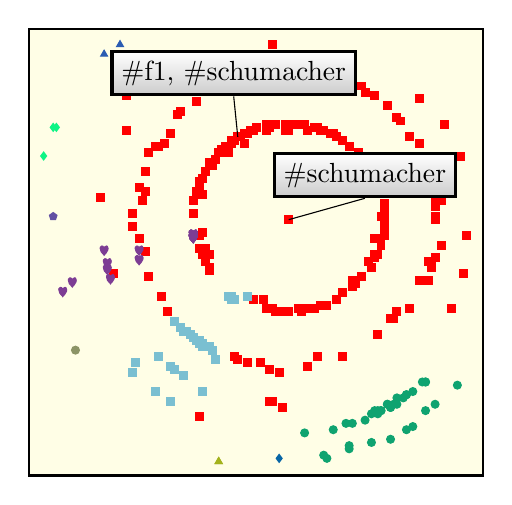
\begin{tikzpicture}[y=\textwidth/3.0,x=\textwidth/3.0, background rectangle/.style={draw=black, thick, fill=yellow!10,},show background rectangle]
\def\marRad{0.5mm}
\definecolor{color0}{rgb}{0.06,0.64,0.44}
\definecolor{color1}{rgb}{1.00,0.00,0.00}
\definecolor{color2}{rgb}{0.17,0.36,0.70}
\definecolor{color3}{rgb}{0.05,0.96,0.52}
\definecolor{color4}{rgb}{0.38,0.31,0.64}
\definecolor{color5}{rgb}{0.49,0.24,0.58}
\definecolor{color6}{rgb}{0.55,0.58,0.40}
\definecolor{color7}{rgb}{0.48,0.75,0.82}
\definecolor{color8}{rgb}{0.64,0.70,0.11}
\definecolor{color9}{rgb}{0.03,0.40,0.65}
\path[fill=color0,draw=color0,mark size=\marRad, mark=*] plot coordinates {(0.21, -0.60)};
\path[fill=color0,draw=color0,mark size=\marRad, mark=*] plot coordinates {(0.13, -0.71)};
\path[fill=color0,draw=color0,mark size=\marRad, mark=*] plot coordinates {(0.54, -0.48)};
\path[fill=color0,draw=color0,mark size=\marRad, mark=*] plot coordinates {(0.27, -0.57)};
\path[fill=color0,draw=color0,mark size=\marRad, mark=*] plot coordinates {(0.32, -0.54)};
\path[fill=color0,draw=color0,mark size=\marRad, mark=*] plot coordinates {(0.32, -0.54)};
\path[fill=color0,draw=color0,mark size=\marRad, mark=*] plot coordinates {(0.19, -0.60)};
\path[fill=color0,draw=color0,mark size=\marRad, mark=*] plot coordinates {(0.25, -0.59)};
\path[fill=color0,draw=color0,mark size=\marRad, mark=*] plot coordinates {(0.40, -0.50)};
\path[fill=color0,draw=color0,mark size=\marRad, mark=*] plot coordinates {(0.43, -0.47)};
\path[fill=color0,draw=color0,mark size=\marRad, mark=*] plot coordinates {(0.30, -0.56)};
\path[fill=color0,draw=color0,mark size=\marRad, mark=*] plot coordinates {(0.15, -0.62)};
\path[fill=color0,draw=color0,mark size=\marRad, mark=*] plot coordinates {(0.20, -0.67)};
\path[fill=color0,draw=color0,mark size=\marRad, mark=*] plot coordinates {(0.28, -0.56)};
\path[fill=color0,draw=color0,mark size=\marRad, mark=*] plot coordinates {(0.37, -0.52)};
\path[fill=color0,draw=color0,mark size=\marRad, mark=*] plot coordinates {(0.38, -0.51)};
\path[fill=color0,draw=color0,mark size=\marRad, mark=*] plot coordinates {(0.29, -0.56)};
\path[fill=color0,draw=color0,mark size=\marRad, mark=*] plot coordinates {(0.34, -0.54)};
\path[fill=color0,draw=color0,mark size=\marRad, mark=*] plot coordinates {(0.30, -0.56)};
\path[fill=color0,draw=color0,mark size=\marRad, mark=*] plot coordinates {(0.44, -0.56)};
\path[fill=color0,draw=color0,mark size=\marRad, mark=*] plot coordinates {(0.47, -0.54)};
\path[fill=color0,draw=color0,mark size=\marRad, mark=*] plot coordinates {(0.44, -0.47)};
\path[fill=color0,draw=color0,mark size=\marRad, mark=*] plot coordinates {(0.44, -0.47)};
\path[fill=color0,draw=color0,mark size=\marRad, mark=*] plot coordinates {(0.38, -0.62)};
\path[fill=color0,draw=color0,mark size=\marRad, mark=*] plot coordinates {(0.06, -0.63)};
\path[fill=color0,draw=color0,mark size=\marRad, mark=*] plot coordinates {(0.33, -0.55)};
\path[fill=color0,draw=color0,mark size=\marRad, mark=*] plot coordinates {(0.33, -0.55)};
\path[fill=color0,draw=color0,mark size=\marRad, mark=*] plot coordinates {(0.35, -0.52)};
\path[fill=color0,draw=color0,mark size=\marRad, mark=*] plot coordinates {(0.20, -0.68)};
\path[fill=color0,draw=color0,mark size=\marRad, mark=*] plot coordinates {(0.38, -0.51)};
\path[fill=color0,draw=color0,mark size=\marRad, mark=*] plot coordinates {(0.35, -0.54)};
\path[fill=color0,draw=color0,mark size=\marRad, mark=*] plot coordinates {(0.27, -0.66)};
\path[fill=color0,draw=color0,mark size=\marRad, mark=*] plot coordinates {(0.12, -0.70)};
\path[fill=color0,draw=color0,mark size=\marRad, mark=*] plot coordinates {(0.29, -0.57)};
\path[fill=color0,draw=color0,mark size=\marRad, mark=*] plot coordinates {(0.40, -0.61)};
\path[fill=color0,draw=color0,mark size=\marRad, mark=*] plot coordinates {(0.33, -0.65)};
\path[fill=color1,draw=color1,mark size=\marRad, mark=square*] plot coordinates {(0.17, 0.46)};
\path[fill=color1,draw=color1,mark size=\marRad, mark=square*] plot coordinates {(0.01, 0.04)};
\path[fill=color1,draw=color1,mark size=\marRad, mark=square*] plot coordinates {(0.31, -0.01)};
\path[fill=color1,draw=color1,mark size=\marRad, mark=square*] plot coordinates {(-0.28, 0.41)};
\path[fill=color1,draw=color1,mark size=\marRad, mark=square*] plot coordinates {(-0.05, 0.49)};
\path[fill=color1,draw=color1,mark size=\marRad, mark=square*] plot coordinates {(0.39, 0.30)};
\path[fill=color1,draw=color1,mark size=\marRad, mark=square*] plot coordinates {(-0.16, -0.39)};
\path[fill=color1,draw=color1,mark size=\marRad, mark=square*] plot coordinates {(0.01, 0.04)};
\path[fill=color1,draw=color1,mark size=\marRad, mark=square*] plot coordinates {(0.01, 0.04)};
\path[fill=color1,draw=color1,mark size=\marRad, mark=square*] plot coordinates {(0.01, 0.04)};
\path[fill=color1,draw=color1,mark size=\marRad, mark=square*] plot coordinates {(0.01, 0.04)};
\path[fill=color1,draw=color1,mark size=\marRad, mark=square*] plot coordinates {(-0.46, -0.02)};
\path[fill=color1,draw=color1,mark size=\marRad, mark=square*] plot coordinates {(-0.25, -0.09)};
\path[fill=color1,draw=color1,mark size=\marRad, mark=square*] plot coordinates {(0.47, 0.12)};
\path[fill=color1,draw=color1,mark size=\marRad, mark=square*] plot coordinates {(0.01, 0.04)};
\path[fill=color1,draw=color1,mark size=\marRad, mark=square*] plot coordinates {(-0.20, 0.26)};
\path[fill=color1,draw=color1,mark size=\marRad, mark=square*] plot coordinates {(0.01, 0.04)};
\path[fill=color1,draw=color1,mark size=\marRad, mark=square*] plot coordinates {(0.01, 0.04)};
\path[fill=color1,draw=color1,mark size=\marRad, mark=square*] plot coordinates {(0.01, 0.04)};
\path[fill=color1,draw=color1,mark size=\marRad, mark=square*] plot coordinates {(0.47, 0.08)};
\path[fill=color1,draw=color1,mark size=\marRad, mark=square*] plot coordinates {(0.01, 0.04)};
\path[fill=color1,draw=color1,mark size=\marRad, mark=square*] plot coordinates {(-0.27, 0.51)};
\path[fill=color1,draw=color1,mark size=\marRad, mark=square*] plot coordinates {(-0.44, 0.13)};
\path[fill=color1,draw=color1,mark size=\marRad, mark=square*] plot coordinates {(-0.39, -0.20)};
\path[fill=color1,draw=color1,mark size=\marRad, mark=square*] plot coordinates {(-0.27, 0.14)};
\path[fill=color1,draw=color1,mark size=\marRad, mark=square*] plot coordinates {(0.01, 0.04)};
\path[fill=color1,draw=color1,mark size=\marRad, mark=square*] plot coordinates {(0.01, 0.04)};
\path[fill=color1,draw=color1,mark size=\marRad, mark=square*] plot coordinates {(0.01, 0.04)};
\path[fill=color1,draw=color1,mark size=\marRad, mark=square*] plot coordinates {(-0.54, -0.13)};
\path[fill=color1,draw=color1,mark size=\marRad, mark=square*] plot coordinates {(0.01, 0.04)};
\path[fill=color1,draw=color1,mark size=\marRad, mark=square*] plot coordinates {(0.01, 0.04)};
\path[fill=color1,draw=color1,mark size=\marRad, mark=square*] plot coordinates {(-0.04, 0.59)};
\path[fill=color1,draw=color1,mark size=\marRad, mark=square*] plot coordinates {(0.01, 0.04)};
\path[fill=color1,draw=color1,mark size=\marRad, mark=square*] plot coordinates {(0.29, -0.32)};
\path[fill=color1,draw=color1,mark size=\marRad, mark=square*] plot coordinates {(0.28, 0.43)};
\path[fill=color1,draw=color1,mark size=\marRad, mark=square*] plot coordinates {(0.47, 0.10)};
\path[fill=color1,draw=color1,mark size=\marRad, mark=square*] plot coordinates {(0.10, 0.33)};
\path[fill=color1,draw=color1,mark size=\marRad, mark=square*] plot coordinates {(0.01, -0.25)};
\path[fill=color1,draw=color1,mark size=\marRad, mark=square*] plot coordinates {(0.01, 0.04)};
\path[fill=color1,draw=color1,mark size=\marRad, mark=square*] plot coordinates {(0.27, -0.11)};
\path[fill=color1,draw=color1,mark size=\marRad, mark=square*] plot coordinates {(0.01, 0.04)};
\path[fill=color1,draw=color1,mark size=\marRad, mark=square*] plot coordinates {(0.50, 0.34)};
\path[fill=color1,draw=color1,mark size=\marRad, mark=square*] plot coordinates {(0.46, 0.13)};
\path[fill=color1,draw=color1,mark size=\marRad, mark=square*] plot coordinates {(0.27, 0.20)};
\path[fill=color1,draw=color1,mark size=\marRad, mark=square*] plot coordinates {(0.01, 0.04)};
\path[fill=color1,draw=color1,mark size=\marRad, mark=square*] plot coordinates {(0.01, 0.04)};
\path[fill=color1,draw=color1,mark size=\marRad, mark=square*] plot coordinates {(0.01, 0.04)};
\path[fill=color1,draw=color1,mark size=\marRad, mark=square*] plot coordinates {(0.01, 0.04)};
\path[fill=color1,draw=color1,mark size=\marRad, mark=square*] plot coordinates {(0.01, 0.04)};
\path[fill=color1,draw=color1,mark size=\marRad, mark=square*] plot coordinates {(0.01, 0.04)};
\path[fill=color1,draw=color1,mark size=\marRad, mark=square*] plot coordinates {(0.01, 0.04)};
\path[fill=color1,draw=color1,mark size=\marRad, mark=square*] plot coordinates {(-0.36, 0.31)};
\path[fill=color1,draw=color1,mark size=\marRad, mark=square*] plot coordinates {(0.01, 0.04)};
\path[fill=color1,draw=color1,mark size=\marRad, mark=square*] plot coordinates {(-0.44, -0.06)};
\path[fill=color1,draw=color1,mark size=\marRad, mark=square*] plot coordinates {(0.56, -0.13)};
\path[fill=color1,draw=color1,mark size=\marRad, mark=square*] plot coordinates {(0.01, 0.04)};
\path[fill=color1,draw=color1,mark size=\marRad, mark=square*] plot coordinates {(0.01, 0.04)};
\path[fill=color1,draw=color1,mark size=\marRad, mark=square*] plot coordinates {(0.11, 0.50)};
\path[fill=color1,draw=color1,mark size=\marRad, mark=square*] plot coordinates {(-0.41, 0.27)};
\path[fill=color1,draw=color1,mark size=\marRad, mark=square*] plot coordinates {(-0.25, 0.19)};
\path[fill=color1,draw=color1,mark size=\marRad, mark=square*] plot coordinates {(0.01, 0.04)};
\path[fill=color1,draw=color1,mark size=\marRad, mark=square*] plot coordinates {(-0.01, -0.55)};
\path[fill=color1,draw=color1,mark size=\marRad, mark=square*] plot coordinates {(0.01, 0.04)};
\path[fill=color1,draw=color1,mark size=\marRad, mark=square*] plot coordinates {(0.26, 0.22)};
\path[fill=color1,draw=color1,mark size=\marRad, mark=square*] plot coordinates {(-0.09, 0.49)};
\path[fill=color1,draw=color1,mark size=\marRad, mark=square*] plot coordinates {(-0.24, -0.12)};
\path[fill=color1,draw=color1,mark size=\marRad, mark=square*] plot coordinates {(0.01, 0.04)};
\path[fill=color1,draw=color1,mark size=\marRad, mark=square*] plot coordinates {(0.01, 0.04)};
\path[fill=color1,draw=color1,mark size=\marRad, mark=square*] plot coordinates {(-0.19, 0.27)};
\path[fill=color1,draw=color1,mark size=\marRad, mark=square*] plot coordinates {(0.07, -0.42)};
\path[fill=color1,draw=color1,mark size=\marRad, mark=square*] plot coordinates {(0.28, -0.08)};
\path[fill=color1,draw=color1,mark size=\marRad, mark=square*] plot coordinates {(0.01, 0.04)};
\path[fill=color1,draw=color1,mark size=\marRad, mark=square*] plot coordinates {(-0.23, 0.21)};
\path[fill=color1,draw=color1,mark size=\marRad, mark=square*] plot coordinates {(0.12, -0.23)};
\path[fill=color1,draw=color1,mark size=\marRad, mark=square*] plot coordinates {(0.01, 0.04)};
\path[fill=color1,draw=color1,mark size=\marRad, mark=square*] plot coordinates {(-0.58, 0.11)};
\path[fill=color1,draw=color1,mark size=\marRad, mark=square*] plot coordinates {(0.01, 0.04)};
\path[fill=color1,draw=color1,mark size=\marRad, mark=square*] plot coordinates {(-0.38, 0.28)};
\path[fill=color1,draw=color1,mark size=\marRad, mark=square*] plot coordinates {(-0.02, -0.44)};
\path[fill=color1,draw=color1,mark size=\marRad, mark=square*] plot coordinates {(0.31, 0.03)};
\path[fill=color1,draw=color1,mark size=\marRad, mark=square*] plot coordinates {(0.01, 0.04)};
\path[fill=color1,draw=color1,mark size=\marRad, mark=square*] plot coordinates {(0.01, 0.04)};
\path[fill=color1,draw=color1,mark size=\marRad, mark=square*] plot coordinates {(0.01, 0.04)};
\path[fill=color1,draw=color1,mark size=\marRad, mark=square*] plot coordinates {(-0.48, 0.02)};
\path[fill=color1,draw=color1,mark size=\marRad, mark=square*] plot coordinates {(0.01, 0.04)};
\path[fill=color1,draw=color1,mark size=\marRad, mark=square*] plot coordinates {(0.18, -0.19)};
\path[fill=color1,draw=color1,mark size=\marRad, mark=square*] plot coordinates {(0.01, 0.04)};
\path[fill=color1,draw=color1,mark size=\marRad, mark=square*] plot coordinates {(0.01, 0.04)};
\path[fill=color1,draw=color1,mark size=\marRad, mark=square*] plot coordinates {(0.01, 0.04)};
\path[fill=color1,draw=color1,mark size=\marRad, mark=square*] plot coordinates {(0.01, 0.04)};
\path[fill=color1,draw=color1,mark size=\marRad, mark=square*] plot coordinates {(0.02, 0.34)};
\path[fill=color1,draw=color1,mark size=\marRad, mark=square*] plot coordinates {(0.01, 0.04)};
\path[fill=color1,draw=color1,mark size=\marRad, mark=square*] plot coordinates {(0.01, 0.04)};
\path[fill=color1,draw=color1,mark size=\marRad, mark=square*] plot coordinates {(0.39, 0.30)};
\path[fill=color1,draw=color1,mark size=\marRad, mark=square*] plot coordinates {(0.01, 0.04)};
\path[fill=color1,draw=color1,mark size=\marRad, mark=square*] plot coordinates {(0.01, 0.04)};
\path[fill=color1,draw=color1,mark size=\marRad, mark=square*] plot coordinates {(0.01, 0.04)};
\path[fill=color1,draw=color1,mark size=\marRad, mark=square*] plot coordinates {(0.01, 0.04)};
\path[fill=color1,draw=color1,mark size=\marRad, mark=square*] plot coordinates {(0.01, 0.04)};
\path[fill=color1,draw=color1,mark size=\marRad, mark=square*] plot coordinates {(-0.27, -0.05)};
\path[fill=color1,draw=color1,mark size=\marRad, mark=square*] plot coordinates {(0.01, 0.04)};
\path[fill=color1,draw=color1,mark size=\marRad, mark=square*] plot coordinates {(0.45, -0.09)};
\path[fill=color1,draw=color1,mark size=\marRad, mark=square*] plot coordinates {(0.01, 0.04)};
\path[fill=color1,draw=color1,mark size=\marRad, mark=square*] plot coordinates {(0.01, 0.04)};
\path[fill=color1,draw=color1,mark size=\marRad, mark=square*] plot coordinates {(0.01, 0.04)};
\path[fill=color1,draw=color1,mark size=\marRad, mark=square*] plot coordinates {(0.42, 0.28)};
\path[fill=color1,draw=color1,mark size=\marRad, mark=square*] plot coordinates {(-0.46, 0.14)};
\path[fill=color1,draw=color1,mark size=\marRad, mark=square*] plot coordinates {(0.47, 0.05)};
\path[fill=color1,draw=color1,mark size=\marRad, mark=square*] plot coordinates {(0.11, 0.32)};
\path[fill=color1,draw=color1,mark size=\marRad, mark=square*] plot coordinates {(0.01, 0.04)};
\path[fill=color1,draw=color1,mark size=\marRad, mark=square*] plot coordinates {(0.01, 0.04)};
\path[fill=color1,draw=color1,mark size=\marRad, mark=square*] plot coordinates {(0.01, 0.04)};
\path[fill=color1,draw=color1,mark size=\marRad, mark=square*] plot coordinates {(0.01, 0.04)};
\path[fill=color1,draw=color1,mark size=\marRad, mark=square*] plot coordinates {(0.11, -0.23)};
\path[fill=color1,draw=color1,mark size=\marRad, mark=square*] plot coordinates {(0.01, 0.04)};
\path[fill=color1,draw=color1,mark size=\marRad, mark=square*] plot coordinates {(0.01, 0.04)};
\path[fill=color1,draw=color1,mark size=\marRad, mark=square*] plot coordinates {(0.01, 0.04)};
\path[fill=color1,draw=color1,mark size=\marRad, mark=square*] plot coordinates {(0.01, 0.04)};
\path[fill=color1,draw=color1,mark size=\marRad, mark=square*] plot coordinates {(0.01, 0.04)};
\path[fill=color1,draw=color1,mark size=\marRad, mark=square*] plot coordinates {(-0.28, 0.13)};
\path[fill=color1,draw=color1,mark size=\marRad, mark=square*] plot coordinates {(0.30, 0.13)};
\path[fill=color1,draw=color1,mark size=\marRad, mark=square*] plot coordinates {(0.49, -0.04)};
\path[fill=color1,draw=color1,mark size=\marRad, mark=square*] plot coordinates {(0.01, 0.04)};
\path[fill=color1,draw=color1,mark size=\marRad, mark=square*] plot coordinates {(0.01, 0.04)};
\path[fill=color1,draw=color1,mark size=\marRad, mark=square*] plot coordinates {(0.01, 0.04)};
\path[fill=color1,draw=color1,mark size=\marRad, mark=square*] plot coordinates {(0.24, 0.46)};
\path[fill=color1,draw=color1,mark size=\marRad, mark=square*] plot coordinates {(0.01, 0.04)};
\path[fill=color1,draw=color1,mark size=\marRad, mark=square*] plot coordinates {(0.01, 0.04)};
\path[fill=color1,draw=color1,mark size=\marRad, mark=square*] plot coordinates {(0.01, 0.04)};
\path[fill=color1,draw=color1,mark size=\marRad, mark=square*] plot coordinates {(0.01, 0.04)};
\path[fill=color1,draw=color1,mark size=\marRad, mark=square*] plot coordinates {(0.01, 0.04)};
\path[fill=color1,draw=color1,mark size=\marRad, mark=square*] plot coordinates {(0.01, 0.04)};
\path[fill=color1,draw=color1,mark size=\marRad, mark=square*] plot coordinates {(0.28, -0.07)};
\path[fill=color1,draw=color1,mark size=\marRad, mark=square*] plot coordinates {(0.01, 0.04)};
\path[fill=color1,draw=color1,mark size=\marRad, mark=square*] plot coordinates {(0.01, 0.04)};
\path[fill=color1,draw=color1,mark size=\marRad, mark=square*] plot coordinates {(0.01, 0.04)};
\path[fill=color1,draw=color1,mark size=\marRad, mark=square*] plot coordinates {(0.01, 0.04)};
\path[fill=color1,draw=color1,mark size=\marRad, mark=square*] plot coordinates {(0.01, 0.04)};
\path[fill=color1,draw=color1,mark size=\marRad, mark=square*] plot coordinates {(-0.17, 0.29)};
\path[fill=color1,draw=color1,mark size=\marRad, mark=square*] plot coordinates {(0.35, 0.36)};
\path[fill=color1,draw=color1,mark size=\marRad, mark=square*] plot coordinates {(0.46, -0.11)};
\path[fill=color1,draw=color1,mark size=\marRad, mark=square*] plot coordinates {(-0.48, 0.06)};
\path[fill=color1,draw=color1,mark size=\marRad, mark=square*] plot coordinates {(0.01, 0.04)};
\path[fill=color1,draw=color1,mark size=\marRad, mark=square*] plot coordinates {(0.30, -0.04)};
\path[fill=color1,draw=color1,mark size=\marRad, mark=square*] plot coordinates {(0.01, 0.04)};
\path[fill=color1,draw=color1,mark size=\marRad, mark=square*] plot coordinates {(0.29, 0.17)};
\path[fill=color1,draw=color1,mark size=\marRad, mark=square*] plot coordinates {(0.01, 0.04)};
\path[fill=color1,draw=color1,mark size=\marRad, mark=square*] plot coordinates {(0.01, 0.04)};
\path[fill=color1,draw=color1,mark size=\marRad, mark=square*] plot coordinates {(0.01, 0.04)};
\path[fill=color1,draw=color1,mark size=\marRad, mark=square*] plot coordinates {(0.01, 0.04)};
\path[fill=color1,draw=color1,mark size=\marRad, mark=square*] plot coordinates {(0.01, 0.04)};
\path[fill=color1,draw=color1,mark size=\marRad, mark=square*] plot coordinates {(0.01, 0.04)};
\path[fill=color1,draw=color1,mark size=\marRad, mark=square*] plot coordinates {(0.01, 0.04)};
\path[fill=color1,draw=color1,mark size=\marRad, mark=square*] plot coordinates {(0.01, 0.04)};
\path[fill=color1,draw=color1,mark size=\marRad, mark=square*] plot coordinates {(-0.05, -0.53)};
\path[fill=color1,draw=color1,mark size=\marRad, mark=square*] plot coordinates {(0.01, 0.04)};
\path[fill=color1,draw=color1,mark size=\marRad, mark=square*] plot coordinates {(0.46, -0.10)};
\path[fill=color1,draw=color1,mark size=\marRad, mark=square*] plot coordinates {(0.01, 0.04)};
\path[fill=color1,draw=color1,mark size=\marRad, mark=square*] plot coordinates {(0.01, 0.04)};
\path[fill=color1,draw=color1,mark size=\marRad, mark=square*] plot coordinates {(-0.29, 0.10)};
\path[fill=color1,draw=color1,mark size=\marRad, mark=square*] plot coordinates {(0.09, -0.24)};
\path[fill=color1,draw=color1,mark size=\marRad, mark=square*] plot coordinates {(0.01, 0.04)};
\path[fill=color1,draw=color1,mark size=\marRad, mark=square*] plot coordinates {(0.01, 0.04)};
\path[fill=color1,draw=color1,mark size=\marRad, mark=square*] plot coordinates {(0.01, 0.04)};
\path[fill=color1,draw=color1,mark size=\marRad, mark=square*] plot coordinates {(0.01, 0.04)};
\path[fill=color1,draw=color1,mark size=\marRad, mark=square*] plot coordinates {(0.01, 0.04)};
\path[fill=color1,draw=color1,mark size=\marRad, mark=square*] plot coordinates {(0.00, 0.34)};
\path[fill=color1,draw=color1,mark size=\marRad, mark=square*] plot coordinates {(0.01, 0.04)};
\path[fill=color1,draw=color1,mark size=\marRad, mark=square*] plot coordinates {(0.01, 0.04)};
\path[fill=color1,draw=color1,mark size=\marRad, mark=square*] plot coordinates {(0.01, 0.04)};
\path[fill=color1,draw=color1,mark size=\marRad, mark=square*] plot coordinates {(0.01, 0.04)};
\path[fill=color1,draw=color1,mark size=\marRad, mark=square*] plot coordinates {(0.01, 0.04)};
\path[fill=color1,draw=color1,mark size=\marRad, mark=square*] plot coordinates {(0.01, 0.04)};
\path[fill=color1,draw=color1,mark size=\marRad, mark=square*] plot coordinates {(0.06, 0.34)};
\path[fill=color1,draw=color1,mark size=\marRad, mark=square*] plot coordinates {(0.01, 0.04)};
\path[fill=color1,draw=color1,mark size=\marRad, mark=square*] plot coordinates {(-0.13, 0.31)};
\path[fill=color1,draw=color1,mark size=\marRad, mark=square*] plot coordinates {(0.01, 0.04)};
\path[fill=color1,draw=color1,mark size=\marRad, mark=square*] plot coordinates {(0.01, 0.04)};
\path[fill=color1,draw=color1,mark size=\marRad, mark=square*] plot coordinates {(-0.44, 0.19)};
\path[fill=color1,draw=color1,mark size=\marRad, mark=square*] plot coordinates {(0.01, 0.04)};
\path[fill=color1,draw=color1,mark size=\marRad, mark=square*] plot coordinates {(0.01, 0.04)};
\path[fill=color1,draw=color1,mark size=\marRad, mark=square*] plot coordinates {(0.31, 0.09)};
\path[fill=color1,draw=color1,mark size=\marRad, mark=square*] plot coordinates {(0.01, 0.04)};
\path[fill=color1,draw=color1,mark size=\marRad, mark=square*] plot coordinates {(0.01, 0.04)};
\path[fill=color1,draw=color1,mark size=\marRad, mark=square*] plot coordinates {(0.01, 0.04)};
\path[fill=color1,draw=color1,mark size=\marRad, mark=square*] plot coordinates {(0.14, 0.31)};
\path[fill=color1,draw=color1,mark size=\marRad, mark=square*] plot coordinates {(0.01, 0.04)};
\path[fill=color1,draw=color1,mark size=\marRad, mark=square*] plot coordinates {(0.29, 0.16)};
\path[fill=color1,draw=color1,mark size=\marRad, mark=square*] plot coordinates {(0.18, 0.29)};
\path[fill=color1,draw=color1,mark size=\marRad, mark=square*] plot coordinates {(0.10, -0.39)};
\path[fill=color1,draw=color1,mark size=\marRad, mark=square*] plot coordinates {(0.01, 0.04)};
\path[fill=color1,draw=color1,mark size=\marRad, mark=square*] plot coordinates {(0.01, 0.04)};
\path[fill=color1,draw=color1,mark size=\marRad, mark=square*] plot coordinates {(0.20, 0.47)};
\path[fill=color1,draw=color1,mark size=\marRad, mark=square*] plot coordinates {(0.01, 0.04)};
\path[fill=color1,draw=color1,mark size=\marRad, mark=square*] plot coordinates {(0.01, 0.04)};
\path[fill=color1,draw=color1,mark size=\marRad, mark=square*] plot coordinates {(0.01, 0.04)};
\path[fill=color1,draw=color1,mark size=\marRad, mark=square*] plot coordinates {(0.01, 0.04)};
\path[fill=color1,draw=color1,mark size=\marRad, mark=square*] plot coordinates {(0.01, 0.04)};
\path[fill=color1,draw=color1,mark size=\marRad, mark=square*] plot coordinates {(0.01, 0.04)};
\path[fill=color1,draw=color1,mark size=\marRad, mark=square*] plot coordinates {(-0.27, -0.01)};
\path[fill=color1,draw=color1,mark size=\marRad, mark=square*] plot coordinates {(0.21, -0.17)};
\path[fill=color1,draw=color1,mark size=\marRad, mark=square*] plot coordinates {(0.01, 0.04)};
\path[fill=color1,draw=color1,mark size=\marRad, mark=square*] plot coordinates {(-0.04, -0.53)};
\path[fill=color1,draw=color1,mark size=\marRad, mark=square*] plot coordinates {(0.01, 0.04)};
\path[fill=color1,draw=color1,mark size=\marRad, mark=square*] plot coordinates {(0.01, 0.04)};
\path[fill=color1,draw=color1,mark size=\marRad, mark=square*] plot coordinates {(0.01, 0.04)};
\path[fill=color1,draw=color1,mark size=\marRad, mark=square*] plot coordinates {(0.31, 0.06)};
\path[fill=color1,draw=color1,mark size=\marRad, mark=square*] plot coordinates {(0.01, 0.04)};
\path[fill=color1,draw=color1,mark size=\marRad, mark=square*] plot coordinates {(0.01, 0.04)};
\path[fill=color1,draw=color1,mark size=\marRad, mark=square*] plot coordinates {(-0.13, 0.49)};
\path[fill=color1,draw=color1,mark size=\marRad, mark=square*] plot coordinates {(0.42, -0.15)};
\path[fill=color1,draw=color1,mark size=\marRad, mark=square*] plot coordinates {(0.30, -0.03)};
\path[fill=color1,draw=color1,mark size=\marRad, mark=square*] plot coordinates {(0.01, 0.04)};
\path[fill=color1,draw=color1,mark size=\marRad, mark=square*] plot coordinates {(0.01, 0.04)};
\path[fill=color1,draw=color1,mark size=\marRad, mark=square*] plot coordinates {(-0.09, 0.33)};
\path[fill=color1,draw=color1,mark size=\marRad, mark=square*] plot coordinates {(0.01, 0.04)};
\path[fill=color1,draw=color1,mark size=\marRad, mark=square*] plot coordinates {(0.01, 0.04)};
\path[fill=color1,draw=color1,mark size=\marRad, mark=square*] plot coordinates {(0.18, -0.39)};
\path[fill=color1,draw=color1,mark size=\marRad, mark=square*] plot coordinates {(-0.14, 0.30)};
\path[fill=color1,draw=color1,mark size=\marRad, mark=square*] plot coordinates {(-0.15, -0.40)};
\path[fill=color1,draw=color1,mark size=\marRad, mark=square*] plot coordinates {(0.31, -0.01)};
\path[fill=color1,draw=color1,mark size=\marRad, mark=square*] plot coordinates {(0.01, 0.04)};
\path[fill=color1,draw=color1,mark size=\marRad, mark=square*] plot coordinates {(0.01, 0.04)};
\path[fill=color1,draw=color1,mark size=\marRad, mark=square*] plot coordinates {(0.01, 0.04)};
\path[fill=color1,draw=color1,mark size=\marRad, mark=square*] plot coordinates {(0.01, 0.04)};
\path[fill=color1,draw=color1,mark size=\marRad, mark=square*] plot coordinates {(0.14, 0.31)};
\path[fill=color1,draw=color1,mark size=\marRad, mark=square*] plot coordinates {(0.20, 0.27)};
\path[fill=color1,draw=color1,mark size=\marRad, mark=square*] plot coordinates {(0.01, 0.04)};
\path[fill=color1,draw=color1,mark size=\marRad, mark=square*] plot coordinates {(0.00, 0.32)};
\path[fill=color1,draw=color1,mark size=\marRad, mark=square*] plot coordinates {(0.01, 0.04)};
\path[fill=color1,draw=color1,mark size=\marRad, mark=square*] plot coordinates {(0.25, 0.20)};
\path[fill=color1,draw=color1,mark size=\marRad, mark=square*] plot coordinates {(0.01, 0.04)};
\path[fill=color1,draw=color1,mark size=\marRad, mark=square*] plot coordinates {(0.01, 0.04)};
\path[fill=color1,draw=color1,mark size=\marRad, mark=square*] plot coordinates {(0.01, 0.04)};
\path[fill=color1,draw=color1,mark size=\marRad, mark=square*] plot coordinates {(0.04, 0.34)};
\path[fill=color1,draw=color1,mark size=\marRad, mark=square*] plot coordinates {(0.28, -0.02)};
\path[fill=color1,draw=color1,mark size=\marRad, mark=square*] plot coordinates {(0.01, 0.04)};
\path[fill=color1,draw=color1,mark size=\marRad, mark=square*] plot coordinates {(0.01, 0.04)};
\path[fill=color1,draw=color1,mark size=\marRad, mark=square*] plot coordinates {(0.01, 0.04)};
\path[fill=color1,draw=color1,mark size=\marRad, mark=square*] plot coordinates {(-0.04, -0.24)};
\path[fill=color1,draw=color1,mark size=\marRad, mark=square*] plot coordinates {(0.01, 0.04)};
\path[fill=color1,draw=color1,mark size=\marRad, mark=square*] plot coordinates {(0.01, 0.04)};
\path[fill=color1,draw=color1,mark size=\marRad, mark=square*] plot coordinates {(0.01, 0.04)};
\path[fill=color1,draw=color1,mark size=\marRad, mark=square*] plot coordinates {(-0.24, -0.07)};
\path[fill=color1,draw=color1,mark size=\marRad, mark=square*] plot coordinates {(0.24, 0.21)};
\path[fill=color1,draw=color1,mark size=\marRad, mark=square*] plot coordinates {(0.28, 0.14)};
\path[fill=color1,draw=color1,mark size=\marRad, mark=square*] plot coordinates {(-0.13, 0.28)};
\path[fill=color1,draw=color1,mark size=\marRad, mark=square*] plot coordinates {(0.01, 0.04)};
\path[fill=color1,draw=color1,mark size=\marRad, mark=square*] plot coordinates {(0.01, 0.04)};
\path[fill=color1,draw=color1,mark size=\marRad, mark=square*] plot coordinates {(0.34, -0.27)};
\path[fill=color1,draw=color1,mark size=\marRad, mark=square*] plot coordinates {(0.16, 0.30)};
\path[fill=color1,draw=color1,mark size=\marRad, mark=square*] plot coordinates {(0.01, 0.04)};
\path[fill=color1,draw=color1,mark size=\marRad, mark=square*] plot coordinates {(0.01, 0.04)};
\path[fill=color1,draw=color1,mark size=\marRad, mark=square*] plot coordinates {(0.01, 0.04)};
\path[fill=color1,draw=color1,mark size=\marRad, mark=square*] plot coordinates {(0.01, 0.04)};
\path[fill=color1,draw=color1,mark size=\marRad, mark=square*] plot coordinates {(0.01, 0.04)};
\path[fill=color1,draw=color1,mark size=\marRad, mark=square*] plot coordinates {(-0.29, 0.06)};
\path[fill=color1,draw=color1,mark size=\marRad, mark=square*] plot coordinates {(0.01, 0.04)};
\path[fill=color1,draw=color1,mark size=\marRad, mark=square*] plot coordinates {(0.20, 0.27)};
\path[fill=color1,draw=color1,mark size=\marRad, mark=square*] plot coordinates {(0.01, 0.04)};
\path[fill=color1,draw=color1,mark size=\marRad, mark=square*] plot coordinates {(0.01, 0.04)};
\path[fill=color1,draw=color1,mark size=\marRad, mark=square*] plot coordinates {(0.01, 0.04)};
\path[fill=color1,draw=color1,mark size=\marRad, mark=square*] plot coordinates {(0.01, 0.04)};
\path[fill=color1,draw=color1,mark size=\marRad, mark=square*] plot coordinates {(0.01, 0.04)};
\path[fill=color1,draw=color1,mark size=\marRad, mark=square*] plot coordinates {(0.16, -0.21)};
\path[fill=color1,draw=color1,mark size=\marRad, mark=square*] plot coordinates {(0.01, 0.04)};
\path[fill=color1,draw=color1,mark size=\marRad, mark=square*] plot coordinates {(0.26, -0.09)};
\path[fill=color1,draw=color1,mark size=\marRad, mark=square*] plot coordinates {(0.07, 0.32)};
\path[fill=color1,draw=color1,mark size=\marRad, mark=square*] plot coordinates {(0.01, 0.04)};
\path[fill=color1,draw=color1,mark size=\marRad, mark=square*] plot coordinates {(0.01, 0.04)};
\path[fill=color1,draw=color1,mark size=\marRad, mark=square*] plot coordinates {(0.01, 0.04)};
\path[fill=color1,draw=color1,mark size=\marRad, mark=square*] plot coordinates {(0.01, 0.04)};
\path[fill=color1,draw=color1,mark size=\marRad, mark=square*] plot coordinates {(0.01, 0.04)};
\path[fill=color1,draw=color1,mark size=\marRad, mark=square*] plot coordinates {(0.01, 0.04)};
\path[fill=color1,draw=color1,mark size=\marRad, mark=square*] plot coordinates {(0.01, 0.04)};
\path[fill=color1,draw=color1,mark size=\marRad, mark=square*] plot coordinates {(0.01, 0.04)};
\path[fill=color1,draw=color1,mark size=\marRad, mark=square*] plot coordinates {(0.01, 0.04)};
\path[fill=color1,draw=color1,mark size=\marRad, mark=square*] plot coordinates {(-0.24, 0.22)};
\path[fill=color1,draw=color1,mark size=\marRad, mark=square*] plot coordinates {(-0.50, 0.32)};
\path[fill=color1,draw=color1,mark size=\marRad, mark=square*] plot coordinates {(0.01, 0.04)};
\path[fill=color1,draw=color1,mark size=\marRad, mark=square*] plot coordinates {(-0.45, 0.10)};
\path[fill=color1,draw=color1,mark size=\marRad, mark=square*] plot coordinates {(-0.29, 0.06)};
\path[fill=color1,draw=color1,mark size=\marRad, mark=square*] plot coordinates {(0.31, 0.08)};
\path[fill=color1,draw=color1,mark size=\marRad, mark=square*] plot coordinates {(0.24, -0.14)};
\path[fill=color1,draw=color1,mark size=\marRad, mark=square*] plot coordinates {(0.01, 0.04)};
\path[fill=color1,draw=color1,mark size=\marRad, mark=square*] plot coordinates {(0.01, 0.04)};
\path[fill=color1,draw=color1,mark size=\marRad, mark=square*] plot coordinates {(-0.07, -0.21)};
\path[fill=color1,draw=color1,mark size=\marRad, mark=square*] plot coordinates {(0.01, 0.04)};
\path[fill=color1,draw=color1,mark size=\marRad, mark=square*] plot coordinates {(0.21, -0.15)};
\path[fill=color1,draw=color1,mark size=\marRad, mark=square*] plot coordinates {(0.01, 0.04)};
\path[fill=color1,draw=color1,mark size=\marRad, mark=square*] plot coordinates {(0.01, 0.04)};
\path[fill=color1,draw=color1,mark size=\marRad, mark=square*] plot coordinates {(0.01, 0.04)};
\path[fill=color1,draw=color1,mark size=\marRad, mark=square*] plot coordinates {(0.01, 0.04)};
\path[fill=color1,draw=color1,mark size=\marRad, mark=square*] plot coordinates {(0.01, 0.04)};
\path[fill=color1,draw=color1,mark size=\marRad, mark=square*] plot coordinates {(0.01, 0.04)};
\path[fill=color1,draw=color1,mark size=\marRad, mark=square*] plot coordinates {(0.01, 0.04)};
\path[fill=color1,draw=color1,mark size=\marRad, mark=square*] plot coordinates {(0.01, 0.04)};
\path[fill=color1,draw=color1,mark size=\marRad, mark=square*] plot coordinates {(0.01, 0.04)};
\path[fill=color1,draw=color1,mark size=\marRad, mark=square*] plot coordinates {(0.01, 0.04)};
\path[fill=color1,draw=color1,mark size=\marRad, mark=square*] plot coordinates {(0.01, 0.04)};
\path[fill=color1,draw=color1,mark size=\marRad, mark=square*] plot coordinates {(0.01, 0.04)};
\path[fill=color1,draw=color1,mark size=\marRad, mark=square*] plot coordinates {(0.22, 0.24)};
\path[fill=color1,draw=color1,mark size=\marRad, mark=square*] plot coordinates {(0.01, 0.04)};
\path[fill=color1,draw=color1,mark size=\marRad, mark=square*] plot coordinates {(0.01, 0.04)};
\path[fill=color1,draw=color1,mark size=\marRad, mark=square*] plot coordinates {(-0.10, 0.32)};
\path[fill=color1,draw=color1,mark size=\marRad, mark=square*] plot coordinates {(0.01, 0.04)};
\path[fill=color1,draw=color1,mark size=\marRad, mark=square*] plot coordinates {(0.18, 0.48)};
\path[fill=color1,draw=color1,mark size=\marRad, mark=square*] plot coordinates {(0.01, 0.04)};
\path[fill=color1,draw=color1,mark size=\marRad, mark=square*] plot coordinates {(0.01, 0.04)};
\path[fill=color1,draw=color1,mark size=\marRad, mark=square*] plot coordinates {(0.01, 0.04)};
\path[fill=color1,draw=color1,mark size=\marRad, mark=square*] plot coordinates {(0.25, 0.44)};
\path[fill=color1,draw=color1,mark size=\marRad, mark=square*] plot coordinates {(0.01, 0.04)};
\path[fill=color1,draw=color1,mark size=\marRad, mark=square*] plot coordinates {(0.01, 0.04)};
\path[fill=color1,draw=color1,mark size=\marRad, mark=square*] plot coordinates {(0.01, 0.04)};
\path[fill=color1,draw=color1,mark size=\marRad, mark=square*] plot coordinates {(-0.10, -0.21)};
\path[fill=color1,draw=color1,mark size=\marRad, mark=square*] plot coordinates {(0.01, -0.25)};
\path[fill=color1,draw=color1,mark size=\marRad, mark=square*] plot coordinates {(0.01, 0.04)};
\path[fill=color1,draw=color1,mark size=\marRad, mark=square*] plot coordinates {(0.01, 0.04)};
\path[fill=color1,draw=color1,mark size=\marRad, mark=square*] plot coordinates {(0.01, 0.04)};
\path[fill=color1,draw=color1,mark size=\marRad, mark=square*] plot coordinates {(0.01, 0.04)};
\path[fill=color1,draw=color1,mark size=\marRad, mark=square*] plot coordinates {(0.01, 0.04)};
\path[fill=color1,draw=color1,mark size=\marRad, mark=square*] plot coordinates {(0.27, 0.17)};
\path[fill=color1,draw=color1,mark size=\marRad, mark=square*] plot coordinates {(-0.27, 0.16)};
\path[fill=color1,draw=color1,mark size=\marRad, mark=square*] plot coordinates {(0.01, 0.04)};
\path[fill=color1,draw=color1,mark size=\marRad, mark=square*] plot coordinates {(0.29, -0.07)};
\path[fill=color1,draw=color1,mark size=\marRad, mark=square*] plot coordinates {(0.01, 0.04)};
\path[fill=color1,draw=color1,mark size=\marRad, mark=square*] plot coordinates {(0.05, -0.25)};
\path[fill=color1,draw=color1,mark size=\marRad, mark=square*] plot coordinates {(0.01, 0.04)};
\path[fill=color1,draw=color1,mark size=\marRad, mark=square*] plot coordinates {(0.01, 0.04)};
\path[fill=color1,draw=color1,mark size=\marRad, mark=square*] plot coordinates {(-0.34, 0.37)};
\path[fill=color1,draw=color1,mark size=\marRad, mark=square*] plot coordinates {(0.01, 0.04)};
\path[fill=color1,draw=color1,mark size=\marRad, mark=square*] plot coordinates {(0.12, 0.32)};
\path[fill=color1,draw=color1,mark size=\marRad, mark=square*] plot coordinates {(0.47, 0.04)};
\path[fill=color1,draw=color1,mark size=\marRad, mark=square*] plot coordinates {(0.01, 0.04)};
\path[fill=color1,draw=color1,mark size=\marRad, mark=square*] plot coordinates {(-0.27, -0.58)};
\path[fill=color1,draw=color1,mark size=\marRad, mark=square*] plot coordinates {(-0.25, -0.05)};
\path[fill=color1,draw=color1,mark size=\marRad, mark=square*] plot coordinates {(0.01, 0.04)};
\path[fill=color1,draw=color1,mark size=\marRad, mark=square*] plot coordinates {(0.01, 0.04)};
\path[fill=color1,draw=color1,mark size=\marRad, mark=square*] plot coordinates {(0.01, 0.04)};
\path[fill=color1,draw=color1,mark size=\marRad, mark=square*] plot coordinates {(0.01, 0.04)};
\path[fill=color1,draw=color1,mark size=\marRad, mark=square*] plot coordinates {(0.01, 0.04)};
\path[fill=color1,draw=color1,mark size=\marRad, mark=square*] plot coordinates {(0.01, 0.04)};
\path[fill=color1,draw=color1,mark size=\marRad, mark=square*] plot coordinates {(0.01, 0.04)};
\path[fill=color1,draw=color1,mark size=\marRad, mark=square*] plot coordinates {(0.01, 0.04)};
\path[fill=color1,draw=color1,mark size=\marRad, mark=square*] plot coordinates {(0.01, 0.04)};
\path[fill=color1,draw=color1,mark size=\marRad, mark=square*] plot coordinates {(-0.31, 0.51)};
\path[fill=color1,draw=color1,mark size=\marRad, mark=square*] plot coordinates {(0.01, 0.04)};
\path[fill=color1,draw=color1,mark size=\marRad, mark=square*] plot coordinates {(0.01, 0.04)};
\path[fill=color1,draw=color1,mark size=\marRad, mark=square*] plot coordinates {(0.23, 0.25)};
\path[fill=color1,draw=color1,mark size=\marRad, mark=square*] plot coordinates {(0.01, 0.04)};
\path[fill=color1,draw=color1,mark size=\marRad, mark=square*] plot coordinates {(0.01, 0.04)};
\path[fill=color1,draw=color1,mark size=\marRad, mark=square*] plot coordinates {(0.01, 0.04)};
\path[fill=color1,draw=color1,mark size=\marRad, mark=square*] plot coordinates {(0.01, 0.04)};
\path[fill=color1,draw=color1,mark size=\marRad, mark=square*] plot coordinates {(0.01, 0.04)};
\path[fill=color1,draw=color1,mark size=\marRad, mark=square*] plot coordinates {(0.01, 0.04)};
\path[fill=color1,draw=color1,mark size=\marRad, mark=square*] plot coordinates {(0.01, 0.04)};
\path[fill=color1,draw=color1,mark size=\marRad, mark=square*] plot coordinates {(-0.17, 0.28)};
\path[fill=color1,draw=color1,mark size=\marRad, mark=square*] plot coordinates {(0.01, 0.04)};
\path[fill=color1,draw=color1,mark size=\marRad, mark=square*] plot coordinates {(0.01, 0.04)};
\path[fill=color1,draw=color1,mark size=\marRad, mark=square*] plot coordinates {(0.01, 0.32)};
\path[fill=color1,draw=color1,mark size=\marRad, mark=square*] plot coordinates {(0.01, 0.04)};
\path[fill=color1,draw=color1,mark size=\marRad, mark=square*] plot coordinates {(0.01, 0.04)};
\path[fill=color1,draw=color1,mark size=\marRad, mark=square*] plot coordinates {(0.01, 0.04)};
\path[fill=color1,draw=color1,mark size=\marRad, mark=square*] plot coordinates {(0.01, 0.04)};
\path[fill=color1,draw=color1,mark size=\marRad, mark=square*] plot coordinates {(0.01, 0.04)};
\path[fill=color1,draw=color1,mark size=\marRad, mark=square*] plot coordinates {(0.01, 0.04)};
\path[fill=color1,draw=color1,mark size=\marRad, mark=square*] plot coordinates {(0.01, 0.04)};
\path[fill=color1,draw=color1,mark size=\marRad, mark=square*] plot coordinates {(0.01, 0.04)};
\path[fill=color1,draw=color1,mark size=\marRad, mark=square*] plot coordinates {(-0.40, 0.27)};
\path[fill=color1,draw=color1,mark size=\marRad, mark=square*] plot coordinates {(0.01, 0.04)};
\path[fill=color1,draw=color1,mark size=\marRad, mark=square*] plot coordinates {(0.01, 0.04)};
\path[fill=color1,draw=color1,mark size=\marRad, mark=square*] plot coordinates {(-0.22, 0.23)};
\path[fill=color1,draw=color1,mark size=\marRad, mark=square*] plot coordinates {(0.01, 0.04)};
\path[fill=color1,draw=color1,mark size=\marRad, mark=square*] plot coordinates {(0.01, 0.04)};
\path[fill=color1,draw=color1,mark size=\marRad, mark=square*] plot coordinates {(0.01, 0.04)};
\path[fill=color1,draw=color1,mark size=\marRad, mark=square*] plot coordinates {(-0.06, 0.34)};
\path[fill=color1,draw=color1,mark size=\marRad, mark=square*] plot coordinates {(0.01, 0.04)};
\path[fill=color1,draw=color1,mark size=\marRad, mark=square*] plot coordinates {(0.31, 0.01)};
\path[fill=color1,draw=color1,mark size=\marRad, mark=square*] plot coordinates {(0.33, -0.27)};
\path[fill=color1,draw=color1,mark size=\marRad, mark=square*] plot coordinates {(0.01, 0.04)};
\path[fill=color1,draw=color1,mark size=\marRad, mark=square*] plot coordinates {(0.01, 0.04)};
\path[fill=color1,draw=color1,mark size=\marRad, mark=square*] plot coordinates {(0.01, 0.04)};
\path[fill=color1,draw=color1,mark size=\marRad, mark=square*] plot coordinates {(0.01, 0.04)};
\path[fill=color1,draw=color1,mark size=\marRad, mark=square*] plot coordinates {(0.42, 0.42)};
\path[fill=color1,draw=color1,mark size=\marRad, mark=square*] plot coordinates {(0.01, 0.04)};
\path[fill=color1,draw=color1,mark size=\marRad, mark=square*] plot coordinates {(0.44, -0.15)};
\path[fill=color1,draw=color1,mark size=\marRad, mark=square*] plot coordinates {(-0.43, 0.25)};
\path[fill=color1,draw=color1,mark size=\marRad, mark=square*] plot coordinates {(0.28, 0.18)};
\path[fill=color1,draw=color1,mark size=\marRad, mark=square*] plot coordinates {(0.01, 0.04)};
\path[fill=color1,draw=color1,mark size=\marRad, mark=square*] plot coordinates {(-0.26, 0.17)};
\path[fill=color1,draw=color1,mark size=\marRad, mark=square*] plot coordinates {(0.46, 0.19)};
\path[fill=color1,draw=color1,mark size=\marRad, mark=square*] plot coordinates {(0.01, 0.04)};
\path[fill=color1,draw=color1,mark size=\marRad, mark=square*] plot coordinates {(0.49, 0.10)};
\path[fill=color1,draw=color1,mark size=\marRad, mark=square*] plot coordinates {(0.01, 0.04)};
\path[fill=color1,draw=color1,mark size=\marRad, mark=square*] plot coordinates {(0.01, 0.04)};
\path[fill=color1,draw=color1,mark size=\marRad, mark=square*] plot coordinates {(0.01, 0.04)};
\path[fill=color1,draw=color1,mark size=\marRad, mark=square*] plot coordinates {(0.06, -0.24)};
\path[fill=color1,draw=color1,mark size=\marRad, mark=square*] plot coordinates {(0.01, 0.04)};
\path[fill=color1,draw=color1,mark size=\marRad, mark=square*] plot coordinates {(0.01, 0.04)};
\path[fill=color1,draw=color1,mark size=\marRad, mark=square*] plot coordinates {(-0.02, -0.25)};
\path[fill=color1,draw=color1,mark size=\marRad, mark=square*] plot coordinates {(0.01, 0.04)};
\path[fill=color1,draw=color1,mark size=\marRad, mark=square*] plot coordinates {(0.01, 0.04)};
\path[fill=color1,draw=color1,mark size=\marRad, mark=square*] plot coordinates {(0.01, 0.04)};
\path[fill=color1,draw=color1,mark size=\marRad, mark=square*] plot coordinates {(0.01, 0.04)};
\path[fill=color1,draw=color1,mark size=\marRad, mark=square*] plot coordinates {(0.55, 0.24)};
\path[fill=color1,draw=color1,mark size=\marRad, mark=square*] plot coordinates {(-0.11, 0.32)};
\path[fill=color1,draw=color1,mark size=\marRad, mark=square*] plot coordinates {(-0.33, 0.38)};
\path[fill=color1,draw=color1,mark size=\marRad, mark=square*] plot coordinates {(0.01, 0.04)};
\path[fill=color1,draw=color1,mark size=\marRad, mark=square*] plot coordinates {(-0.05, 0.34)};
\path[fill=color1,draw=color1,mark size=\marRad, mark=square*] plot coordinates {(0.01, 0.04)};
\path[fill=color1,draw=color1,mark size=\marRad, mark=square*] plot coordinates {(0.01, 0.04)};
\path[fill=color1,draw=color1,mark size=\marRad, mark=square*] plot coordinates {(0.01, 0.04)};
\path[fill=color1,draw=color1,mark size=\marRad, mark=square*] plot coordinates {(-0.27, -0.58)};
\path[fill=color1,draw=color1,mark size=\marRad, mark=square*] plot coordinates {(0.01, 0.04)};
\path[fill=color1,draw=color1,mark size=\marRad, mark=square*] plot coordinates {(0.01, 0.04)};
\path[fill=color1,draw=color1,mark size=\marRad, mark=square*] plot coordinates {(0.01, 0.04)};
\path[fill=color1,draw=color1,mark size=\marRad, mark=square*] plot coordinates {(0.01, 0.04)};
\path[fill=color1,draw=color1,mark size=\marRad, mark=square*] plot coordinates {(0.01, 0.04)};
\path[fill=color1,draw=color1,mark size=\marRad, mark=square*] plot coordinates {(0.01, 0.04)};
\path[fill=color1,draw=color1,mark size=\marRad, mark=square*] plot coordinates {(0.01, 0.04)};
\path[fill=color1,draw=color1,mark size=\marRad, mark=square*] plot coordinates {(0.01, 0.04)};
\path[fill=color1,draw=color1,mark size=\marRad, mark=square*] plot coordinates {(0.01, 0.04)};
\path[fill=color1,draw=color1,mark size=\marRad, mark=square*] plot coordinates {(0.30, 0.05)};
\path[fill=color1,draw=color1,mark size=\marRad, mark=square*] plot coordinates {(-0.03, 0.34)};
\path[fill=color1,draw=color1,mark size=\marRad, mark=square*] plot coordinates {(0.01, 0.04)};
\path[fill=color1,draw=color1,mark size=\marRad, mark=square*] plot coordinates {(0.01, 0.04)};
\path[fill=color1,draw=color1,mark size=\marRad, mark=square*] plot coordinates {(0.01, 0.04)};
\path[fill=color1,draw=color1,mark size=\marRad, mark=square*] plot coordinates {(0.52, -0.24)};
\path[fill=color1,draw=color1,mark size=\marRad, mark=square*] plot coordinates {(-0.26, -0.00)};
\path[fill=color1,draw=color1,mark size=\marRad, mark=square*] plot coordinates {(0.01, 0.04)};
\path[fill=color1,draw=color1,mark size=\marRad, mark=square*] plot coordinates {(0.01, 0.04)};
\path[fill=color1,draw=color1,mark size=\marRad, mark=square*] plot coordinates {(0.01, 0.04)};
\path[fill=color1,draw=color1,mark size=\marRad, mark=square*] plot coordinates {(0.30, 0.15)};
\path[fill=color1,draw=color1,mark size=\marRad, mark=square*] plot coordinates {(0.01, 0.04)};
\path[fill=color1,draw=color1,mark size=\marRad, mark=square*] plot coordinates {(0.01, 0.04)};
\path[fill=color1,draw=color1,mark size=\marRad, mark=square*] plot coordinates {(0.01, 0.04)};
\path[fill=color1,draw=color1,mark size=\marRad, mark=square*] plot coordinates {(0.01, 0.04)};
\path[fill=color1,draw=color1,mark size=\marRad, mark=square*] plot coordinates {(0.01, 0.04)};
\path[fill=color1,draw=color1,mark size=\marRad, mark=square*] plot coordinates {(0.01, 0.04)};
\path[fill=color1,draw=color1,mark size=\marRad, mark=square*] plot coordinates {(-0.05, -0.43)};
\path[fill=color1,draw=color1,mark size=\marRad, mark=square*] plot coordinates {(-0.06, 0.32)};
\path[fill=color1,draw=color1,mark size=\marRad, mark=square*] plot coordinates {(0.01, 0.04)};
\path[fill=color1,draw=color1,mark size=\marRad, mark=square*] plot coordinates {(0.01, 0.04)};
\path[fill=color1,draw=color1,mark size=\marRad, mark=square*] plot coordinates {(0.30, -0.02)};
\path[fill=color1,draw=color1,mark size=\marRad, mark=square*] plot coordinates {(-0.09, 0.33)};
\path[fill=color1,draw=color1,mark size=\marRad, mark=square*] plot coordinates {(0.01, 0.04)};
\path[fill=color1,draw=color1,mark size=\marRad, mark=square*] plot coordinates {(0.01, 0.04)};
\path[fill=color1,draw=color1,mark size=\marRad, mark=square*] plot coordinates {(-0.16, 0.29)};
\path[fill=color1,draw=color1,mark size=\marRad, mark=square*] plot coordinates {(0.47, -0.08)};
\path[fill=color1,draw=color1,mark size=\marRad, mark=square*] plot coordinates {(0.57, -0.01)};
\path[fill=color1,draw=color1,mark size=\marRad, mark=square*] plot coordinates {(0.01, 0.04)};
\path[fill=color1,draw=color1,mark size=\marRad, mark=square*] plot coordinates {(0.09, 0.49)};
\path[fill=color1,draw=color1,mark size=\marRad, mark=square*] plot coordinates {(0.01, 0.04)};
\path[fill=color1,draw=color1,mark size=\marRad, mark=square*] plot coordinates {(0.01, 0.04)};
\path[fill=color1,draw=color1,mark size=\marRad, mark=square*] plot coordinates {(0.01, 0.04)};
\path[fill=color1,draw=color1,mark size=\marRad, mark=square*] plot coordinates {(0.15, 0.47)};
\path[fill=color1,draw=color1,mark size=\marRad, mark=square*] plot coordinates {(0.01, 0.04)};
\path[fill=color1,draw=color1,mark size=\marRad, mark=square*] plot coordinates {(0.08, -0.24)};
\path[fill=color1,draw=color1,mark size=\marRad, mark=square*] plot coordinates {(0.01, 0.04)};
\path[fill=color1,draw=color1,mark size=\marRad, mark=square*] plot coordinates {(0.01, 0.04)};
\path[fill=color1,draw=color1,mark size=\marRad, mark=square*] plot coordinates {(0.01, 0.04)};
\path[fill=color1,draw=color1,mark size=\marRad, mark=square*] plot coordinates {(0.01, 0.04)};
\path[fill=color1,draw=color1,mark size=\marRad, mark=square*] plot coordinates {(0.01, 0.04)};
\path[fill=color1,draw=color1,mark size=\marRad, mark=square*] plot coordinates {(-0.18, 0.25)};
\path[fill=color1,draw=color1,mark size=\marRad, mark=square*] plot coordinates {(-0.50, 0.43)};
\path[fill=color1,draw=color1,mark size=\marRad, mark=square*] plot coordinates {(0.01, 0.04)};
\path[fill=color1,draw=color1,mark size=\marRad, mark=square*] plot coordinates {(0.01, 0.04)};
\path[fill=color1,draw=color1,mark size=\marRad, mark=square*] plot coordinates {(0.01, 0.04)};
\path[fill=color1,draw=color1,mark size=\marRad, mark=square*] plot coordinates {(0.01, 0.04)};
\path[fill=color1,draw=color1,mark size=\marRad, mark=square*] plot coordinates {(-0.20, 0.25)};
\path[fill=color1,draw=color1,mark size=\marRad, mark=square*] plot coordinates {(0.01, 0.04)};
\path[fill=color1,draw=color1,mark size=\marRad, mark=square*] plot coordinates {(-0.05, 0.33)};
\path[fill=color1,draw=color1,mark size=\marRad, mark=square*] plot coordinates {(0.01, 0.04)};
\path[fill=color1,draw=color1,mark size=\marRad, mark=square*] plot coordinates {(0.01, 0.04)};
\path[fill=color1,draw=color1,mark size=\marRad, mark=square*] plot coordinates {(0.01, 0.04)};
\path[fill=color1,draw=color1,mark size=\marRad, mark=square*] plot coordinates {(0.01, 0.04)};
\path[fill=color1,draw=color1,mark size=\marRad, mark=square*] plot coordinates {(0.01, 0.04)};
\path[fill=color1,draw=color1,mark size=\marRad, mark=square*] plot coordinates {(0.36, 0.35)};
\path[fill=color1,draw=color1,mark size=\marRad, mark=square*] plot coordinates {(0.01, 0.04)};
\path[fill=color1,draw=color1,mark size=\marRad, mark=square*] plot coordinates {(0.01, 0.04)};
\path[fill=color1,draw=color1,mark size=\marRad, mark=square*] plot coordinates {(0.13, -0.23)};
\path[fill=color1,draw=color1,mark size=\marRad, mark=square*] plot coordinates {(-0.24, -0.11)};
\path[fill=color1,draw=color1,mark size=\marRad, mark=square*] plot coordinates {(-0.08, -0.41)};
\path[fill=color1,draw=color1,mark size=\marRad, mark=square*] plot coordinates {(0.01, 0.04)};
\path[fill=color1,draw=color1,mark size=\marRad, mark=square*] plot coordinates {(0.01, 0.04)};
\path[fill=color1,draw=color1,mark size=\marRad, mark=square*] plot coordinates {(0.01, 0.04)};
\path[fill=color1,draw=color1,mark size=\marRad, mark=square*] plot coordinates {(0.32, 0.40)};
\path[fill=color1,draw=color1,mark size=\marRad, mark=square*] plot coordinates {(0.01, 0.04)};
\path[fill=color1,draw=color1,mark size=\marRad, mark=square*] plot coordinates {(0.01, 0.04)};
\path[fill=color1,draw=color1,mark size=\marRad, mark=square*] plot coordinates {(0.01, 0.04)};
\path[fill=color1,draw=color1,mark size=\marRad, mark=square*] plot coordinates {(0.01, 0.04)};
\path[fill=color1,draw=color1,mark size=\marRad, mark=square*] plot coordinates {(-0.21, 0.25)};
\path[fill=color1,draw=color1,mark size=\marRad, mark=square*] plot coordinates {(0.22, -0.16)};
\path[fill=color1,draw=color1,mark size=\marRad, mark=square*] plot coordinates {(0.01, 0.04)};
\path[fill=color1,draw=color1,mark size=\marRad, mark=square*] plot coordinates {(0.01, 0.04)};
\path[fill=color1,draw=color1,mark size=\marRad, mark=square*] plot coordinates {(0.01, 0.04)};
\path[fill=color1,draw=color1,mark size=\marRad, mark=square*] plot coordinates {(0.01, 0.04)};
\path[fill=color1,draw=color1,mark size=\marRad, mark=square*] plot coordinates {(0.01, 0.04)};
\path[fill=color1,draw=color1,mark size=\marRad, mark=square*] plot coordinates {(0.01, 0.04)};
\path[fill=color1,draw=color1,mark size=\marRad, mark=square*] plot coordinates {(0.01, 0.04)};
\path[fill=color1,draw=color1,mark size=\marRad, mark=square*] plot coordinates {(0.01, 0.04)};
\path[fill=color1,draw=color1,mark size=\marRad, mark=square*] plot coordinates {(0.01, 0.04)};
\path[fill=color1,draw=color1,mark size=\marRad, mark=square*] plot coordinates {(0.01, 0.04)};
\path[fill=color1,draw=color1,mark size=\marRad, mark=square*] plot coordinates {(0.01, 0.04)};
\path[fill=color1,draw=color1,mark size=\marRad, mark=square*] plot coordinates {(0.01, 0.04)};
\path[fill=color1,draw=color1,mark size=\marRad, mark=square*] plot coordinates {(0.02, 0.34)};
\path[fill=color1,draw=color1,mark size=\marRad, mark=square*] plot coordinates {(0.01, 0.04)};
\path[fill=color1,draw=color1,mark size=\marRad, mark=square*] plot coordinates {(0.05, 0.34)};
\path[fill=color1,draw=color1,mark size=\marRad, mark=square*] plot coordinates {(0.01, 0.04)};
\path[fill=color1,draw=color1,mark size=\marRad, mark=square*] plot coordinates {(0.01, 0.04)};
\path[fill=color1,draw=color1,mark size=\marRad, mark=square*] plot coordinates {(-0.26, -0.07)};
\path[fill=color1,draw=color1,mark size=\marRad, mark=square*] plot coordinates {(0.15, 0.31)};
\path[fill=color1,draw=color1,mark size=\marRad, mark=square*] plot coordinates {(-0.02, -0.25)};
\path[fill=color1,draw=color1,mark size=\marRad, mark=square*] plot coordinates {(0.01, 0.04)};
\path[fill=color1,draw=color1,mark size=\marRad, mark=square*] plot coordinates {(0.01, 0.04)};
\path[fill=color1,draw=color1,mark size=\marRad, mark=square*] plot coordinates {(0.01, 0.04)};
\path[fill=color1,draw=color1,mark size=\marRad, mark=square*] plot coordinates {(-0.37, -0.25)};
\path[fill=color1,draw=color1,mark size=\marRad, mark=square*] plot coordinates {(0.01, 0.04)};
\path[fill=color1,draw=color1,mark size=\marRad, mark=square*] plot coordinates {(-0.43, -0.14)};
\path[fill=color1,draw=color1,mark size=\marRad, mark=square*] plot coordinates {(0.01, 0.04)};
\path[fill=color1,draw=color1,mark size=\marRad, mark=square*] plot coordinates {(0.01, 0.04)};
\path[fill=color1,draw=color1,mark size=\marRad, mark=square*] plot coordinates {(0.01, 0.04)};
\path[fill=color1,draw=color1,mark size=\marRad, mark=square*] plot coordinates {(0.01, 0.04)};
\path[fill=color1,draw=color1,mark size=\marRad, mark=square*] plot coordinates {(0.35, -0.25)};
\path[fill=color1,draw=color1,mark size=\marRad, mark=square*] plot coordinates {(0.01, 0.04)};
\path[fill=color1,draw=color1,mark size=\marRad, mark=square*] plot coordinates {(0.01, 0.04)};
\path[fill=color1,draw=color1,mark size=\marRad, mark=square*] plot coordinates {(-0.27, 0.15)};
\path[fill=color1,draw=color1,mark size=\marRad, mark=square*] plot coordinates {(0.01, 0.04)};
\path[fill=color1,draw=color1,mark size=\marRad, mark=square*] plot coordinates {(0.01, 0.04)};
\path[fill=color1,draw=color1,mark size=\marRad, mark=square*] plot coordinates {(-0.12, 0.31)};
\path[fill=color1,draw=color1,mark size=\marRad, mark=square*] plot coordinates {(0.01, 0.04)};
\path[fill=color1,draw=color1,mark size=\marRad, mark=square*] plot coordinates {(0.01, 0.04)};
\path[fill=color1,draw=color1,mark size=\marRad, mark=square*] plot coordinates {(0.01, 0.04)};
\path[fill=color1,draw=color1,mark size=\marRad, mark=square*] plot coordinates {(0.31, 0.05)};
\path[fill=color1,draw=color1,mark size=\marRad, mark=square*] plot coordinates {(0.01, 0.04)};
\path[fill=color1,draw=color1,mark size=\marRad, mark=square*] plot coordinates {(0.01, 0.04)};
\path[fill=color1,draw=color1,mark size=\marRad, mark=square*] plot coordinates {(0.01, 0.04)};
\path[fill=color1,draw=color1,mark size=\marRad, mark=square*] plot coordinates {(0.01, 0.04)};
\path[fill=color1,draw=color1,mark size=\marRad, mark=square*] plot coordinates {(-0.26, 0.12)};
\path[fill=color1,draw=color1,mark size=\marRad, mark=square*] plot coordinates {(-0.03, -0.25)};
\path[fill=color1,draw=color1,mark size=\marRad, mark=square*] plot coordinates {(0.01, 0.04)};
\path[fill=color1,draw=color1,mark size=\marRad, mark=square*] plot coordinates {(0.23, 0.24)};
\path[fill=color1,draw=color1,mark size=\marRad, mark=square*] plot coordinates {(0.04, -0.24)};
\path[fill=color1,draw=color1,mark size=\marRad, mark=square*] plot coordinates {(-0.28, 0.12)};
\path[fill=color1,draw=color1,mark size=\marRad, mark=square*] plot coordinates {(0.23, 0.24)};
\path[fill=color1,draw=color1,mark size=\marRad, mark=square*] plot coordinates {(0.01, 0.04)};
\path[fill=color1,draw=color1,mark size=\marRad, mark=square*] plot coordinates {(0.01, 0.04)};
\path[fill=color1,draw=color1,mark size=\marRad, mark=square*] plot coordinates {(0.01, 0.04)};
\path[fill=color1,draw=color1,mark size=\marRad, mark=square*] plot coordinates {(0.01, 0.04)};
\path[fill=color1,draw=color1,mark size=\marRad, mark=square*] plot coordinates {(0.01, 0.04)};
\path[fill=color1,draw=color1,mark size=\marRad, mark=square*] plot coordinates {(0.01, 0.04)};
\path[fill=color1,draw=color1,mark size=\marRad, mark=square*] plot coordinates {(0.01, 0.04)};
\path[fill=color1,draw=color1,mark size=\marRad, mark=square*] plot coordinates {(-0.06, -0.24)};
\path[fill=color1,draw=color1,mark size=\marRad, mark=square*] plot coordinates {(0.01, 0.04)};
\path[fill=color1,draw=color1,mark size=\marRad, mark=square*] plot coordinates {(0.01, 0.04)};
\path[fill=color1,draw=color1,mark size=\marRad, mark=square*] plot coordinates {(0.01, 0.04)};
\path[fill=color1,draw=color1,mark size=\marRad, mark=square*] plot coordinates {(0.01, 0.04)};
\path[fill=color1,draw=color1,mark size=\marRad, mark=square*] plot coordinates {(0.01, 0.04)};
\path[fill=color1,draw=color1,mark size=\marRad, mark=square*] plot coordinates {(0.01, 0.04)};
\path[fill=color1,draw=color1,mark size=\marRad, mark=square*] plot coordinates {(0.01, 0.04)};
\path[fill=color1,draw=color1,mark size=\marRad, mark=square*] plot coordinates {(0.01, 0.04)};
\path[fill=color1,draw=color1,mark size=\marRad, mark=square*] plot coordinates {(0.01, 0.04)};
\path[fill=color1,draw=color1,mark size=\marRad, mark=square*] plot coordinates {(0.01, 0.04)};
\path[fill=color1,draw=color1,mark size=\marRad, mark=square*] plot coordinates {(0.01, 0.04)};
\path[fill=color1,draw=color1,mark size=\marRad, mark=square*] plot coordinates {(0.01, 0.04)};
\path[fill=color1,draw=color1,mark size=\marRad, mark=square*] plot coordinates {(0.01, 0.04)};
\path[fill=color1,draw=color1,mark size=\marRad, mark=square*] plot coordinates {(0.01, 0.04)};
\path[fill=color1,draw=color1,mark size=\marRad, mark=square*] plot coordinates {(0.01, 0.04)};
\path[fill=color1,draw=color1,mark size=\marRad, mark=square*] plot coordinates {(0.01, 0.04)};
\path[fill=color1,draw=color1,mark size=\marRad, mark=square*] plot coordinates {(0.01, 0.04)};
\path[fill=color1,draw=color1,mark size=\marRad, mark=square*] plot coordinates {(0.01, 0.04)};
\path[fill=color1,draw=color1,mark size=\marRad, mark=square*] plot coordinates {(0.01, 0.04)};
\path[fill=color1,draw=color1,mark size=\marRad, mark=square*] plot coordinates {(0.01, 0.04)};
\path[fill=color1,draw=color1,mark size=\marRad, mark=square*] plot coordinates {(0.01, 0.04)};
\path[fill=color1,draw=color1,mark size=\marRad, mark=square*] plot coordinates {(0.01, 0.04)};
\path[fill=color1,draw=color1,mark size=\marRad, mark=square*] plot coordinates {(0.01, 0.04)};
\path[fill=color1,draw=color1,mark size=\marRad, mark=square*] plot coordinates {(0.01, 0.04)};
\path[fill=color1,draw=color1,mark size=\marRad, mark=square*] plot coordinates {(0.01, 0.04)};
\path[fill=color1,draw=color1,mark size=\marRad, mark=square*] plot coordinates {(0.01, 0.04)};
\path[fill=color1,draw=color1,mark size=\marRad, mark=square*] plot coordinates {(0.01, 0.04)};
\path[fill=color1,draw=color1,mark size=\marRad, mark=square*] plot coordinates {(0.01, 0.04)};
\path[fill=color1,draw=color1,mark size=\marRad, mark=square*] plot coordinates {(0.01, 0.04)};
\path[fill=color1,draw=color1,mark size=\marRad, mark=square*] plot coordinates {(0.01, 0.04)};
\path[fill=color1,draw=color1,mark size=\marRad, mark=square*] plot coordinates {(0.01, 0.04)};
\path[fill=color1,draw=color1,mark size=\marRad, mark=square*] plot coordinates {(0.01, 0.04)};
\path[fill=color1,draw=color1,mark size=\marRad, mark=square*] plot coordinates {(0.01, 0.04)};
\path[fill=color1,draw=color1,mark size=\marRad, mark=square*] plot coordinates {(0.01, 0.04)};
\path[fill=color1,draw=color1,mark size=\marRad, mark=square*] plot coordinates {(-0.15, 0.30)};
\path[fill=color1,draw=color1,mark size=\marRad, mark=square*] plot coordinates {(0.01, 0.04)};
\path[fill=color1,draw=color1,mark size=\marRad, mark=square*] plot coordinates {(0.01, 0.04)};
\path[fill=color1,draw=color1,mark size=\marRad, mark=square*] plot coordinates {(0.01, 0.04)};
\path[fill=color1,draw=color1,mark size=\marRad, mark=square*] plot coordinates {(0.01, 0.04)};
\path[fill=color1,draw=color1,mark size=\marRad, mark=square*] plot coordinates {(0.01, 0.04)};
\path[fill=color1,draw=color1,mark size=\marRad, mark=square*] plot coordinates {(0.01, 0.04)};
\path[fill=color1,draw=color1,mark size=\marRad, mark=square*] plot coordinates {(0.01, 0.04)};
\path[fill=color1,draw=color1,mark size=\marRad, mark=square*] plot coordinates {(0.01, 0.04)};
\path[fill=color1,draw=color1,mark size=\marRad, mark=square*] plot coordinates {(0.01, 0.04)};
\path[fill=color1,draw=color1,mark size=\marRad, mark=square*] plot coordinates {(0.01, 0.04)};
\path[fill=color1,draw=color1,mark size=\marRad, mark=square*] plot coordinates {(0.01, 0.04)};
\path[fill=color1,draw=color1,mark size=\marRad, mark=square*] plot coordinates {(0.01, 0.04)};
\path[fill=color1,draw=color1,mark size=\marRad, mark=square*] plot coordinates {(0.31, 0.02)};
\path[fill=color1,draw=color1,mark size=\marRad, mark=square*] plot coordinates {(0.01, 0.04)};
\path[fill=color1,draw=color1,mark size=\marRad, mark=square*] plot coordinates {(0.01, 0.04)};
\path[fill=color1,draw=color1,mark size=\marRad, mark=square*] plot coordinates {(0.01, 0.04)};
\path[fill=color1,draw=color1,mark size=\marRad, mark=square*] plot coordinates {(0.01, 0.04)};
\path[fill=color1,draw=color1,mark size=\marRad, mark=square*] plot coordinates {(0.01, 0.04)};
\path[fill=color1,draw=color1,mark size=\marRad, mark=square*] plot coordinates {(0.01, 0.04)};
\path[fill=color1,draw=color1,mark size=\marRad, mark=square*] plot coordinates {(0.01, 0.04)};
\path[fill=color1,draw=color1,mark size=\marRad, mark=square*] plot coordinates {(0.01, 0.04)};
\path[fill=color1,draw=color1,mark size=\marRad, mark=square*] plot coordinates {(0.28, 0.13)};
\path[fill=color1,draw=color1,mark size=\marRad, mark=square*] plot coordinates {(0.01, 0.04)};
\path[fill=color1,draw=color1,mark size=\marRad, mark=square*] plot coordinates {(0.01, 0.04)};
\path[fill=color1,draw=color1,mark size=\marRad, mark=square*] plot coordinates {(0.01, 0.04)};
\path[fill=color1,draw=color1,mark size=\marRad, mark=square*] plot coordinates {(0.01, 0.04)};
\path[fill=color1,draw=color1,mark size=\marRad, mark=square*] plot coordinates {(0.01, 0.04)};
\path[fill=color1,draw=color1,mark size=\marRad, mark=square*] plot coordinates {(0.01, 0.04)};
\path[fill=color1,draw=color1,mark size=\marRad, mark=square*] plot coordinates {(0.01, 0.04)};
\path[fill=color1,draw=color1,mark size=\marRad, mark=square*] plot coordinates {(0.45, -0.15)};
\path[fill=color1,draw=color1,mark size=\marRad, mark=square*] plot coordinates {(0.01, 0.04)};
\path[fill=color1,draw=color1,mark size=\marRad, mark=square*] plot coordinates {(0.01, 0.04)};
\path[fill=color1,draw=color1,mark size=\marRad, mark=square*] plot coordinates {(0.01, 0.04)};
\path[fill=color1,draw=color1,mark size=\marRad, mark=square*] plot coordinates {(0.01, 0.04)};
\path[fill=color1,draw=color1,mark size=\marRad, mark=square*] plot coordinates {(-0.26, 0.12)};
\path[fill=color1,draw=color1,mark size=\marRad, mark=square*] plot coordinates {(0.01, 0.04)};
\path[fill=color1,draw=color1,mark size=\marRad, mark=square*] plot coordinates {(0.01, 0.04)};
\path[fill=color1,draw=color1,mark size=\marRad, mark=square*] plot coordinates {(0.39, -0.24)};
\path[fill=color1,draw=color1,mark size=\marRad, mark=square*] plot coordinates {(0.01, 0.04)};
\path[fill=color1,draw=color1,mark size=\marRad, mark=square*] plot coordinates {(0.01, 0.04)};
\path[fill=color1,draw=color1,mark size=\marRad, mark=square*] plot coordinates {(0.01, 0.04)};
\path[fill=color1,draw=color1,mark size=\marRad, mark=square*] plot coordinates {(0.01, 0.04)};
\path[fill=color1,draw=color1,mark size=\marRad, mark=square*] plot coordinates {(0.09, 0.33)};
\path[fill=color1,draw=color1,mark size=\marRad, mark=square*] plot coordinates {(0.01, 0.04)};
\path[fill=color1,draw=color1,mark size=\marRad, mark=square*] plot coordinates {(0.01, 0.04)};
\path[fill=color1,draw=color1,mark size=\marRad, mark=square*] plot coordinates {(-0.03, 0.34)};
\path[fill=color1,draw=color1,mark size=\marRad, mark=square*] plot coordinates {(-0.12, -0.41)};
\path[fill=color7,draw=color7,mark size=\marRad, mark=square*] plot coordinates {(-0.16, -0.21)};
\path[fill=color7,draw=color7,mark size=\marRad, mark=square*] plot coordinates {(-0.18, -0.20)};
\path[fill=color7,draw=color7,mark size=\marRad, mark=square*] plot coordinates {(-0.17, -0.20)};
\path[fill=color7,draw=color7,mark size=\marRad, mark=square*] plot coordinates {(-0.17, -0.20)};
\path[fill=color7,draw=color7,mark size=\marRad, mark=square*] plot coordinates {(-0.40, -0.39)};
\path[fill=color7,draw=color7,mark size=\marRad, mark=square*] plot coordinates {(-0.40, -0.39)};
\path[fill=color7,draw=color7,mark size=\marRad, mark=square*] plot coordinates {(-0.25, -0.36)};
\path[fill=color7,draw=color7,mark size=\marRad, mark=square*] plot coordinates {(-0.17, -0.20)};
\path[fill=color7,draw=color7,mark size=\marRad, mark=square*] plot coordinates {(-0.17, -0.20)};
\path[fill=color7,draw=color7,mark size=\marRad, mark=square*] plot coordinates {(-0.26, -0.50)};
\path[fill=color7,draw=color7,mark size=\marRad, mark=square*] plot coordinates {(-0.27, -0.35)};
\path[fill=color7,draw=color7,mark size=\marRad, mark=square*] plot coordinates {(-0.28, -0.34)};
\path[fill=color7,draw=color7,mark size=\marRad, mark=square*] plot coordinates {(-0.23, -0.37)};
\path[fill=color7,draw=color7,mark size=\marRad, mark=square*] plot coordinates {(-0.17, -0.20)};
\path[fill=color7,draw=color7,mark size=\marRad, mark=square*] plot coordinates {(-0.32, -0.45)};
\path[fill=color7,draw=color7,mark size=\marRad, mark=square*] plot coordinates {(-0.26, -0.36)};
\path[fill=color7,draw=color7,mark size=\marRad, mark=square*] plot coordinates {(-0.17, -0.20)};
\path[fill=color7,draw=color7,mark size=\marRad, mark=square*] plot coordinates {(-0.18, -0.20)};
\path[fill=color7,draw=color7,mark size=\marRad, mark=square*] plot coordinates {(-0.17, -0.20)};
\path[fill=color7,draw=color7,mark size=\marRad, mark=square*] plot coordinates {(-0.17, -0.20)};
\path[fill=color7,draw=color7,mark size=\marRad, mark=square*] plot coordinates {(-0.18, -0.20)};
\path[fill=color7,draw=color7,mark size=\marRad, mark=square*] plot coordinates {(-0.31, -0.31)};
\path[fill=color7,draw=color7,mark size=\marRad, mark=square*] plot coordinates {(-0.17, -0.20)};
\path[fill=color7,draw=color7,mark size=\marRad, mark=square*] plot coordinates {(-0.17, -0.21)};
\path[fill=color7,draw=color7,mark size=\marRad, mark=square*] plot coordinates {(-0.18, -0.20)};
\path[fill=color7,draw=color7,mark size=\marRad, mark=square*] plot coordinates {(-0.17, -0.20)};
\path[fill=color7,draw=color7,mark size=\marRad, mark=square*] plot coordinates {(-0.47, -0.41)};
\path[fill=color7,draw=color7,mark size=\marRad, mark=square*] plot coordinates {(-0.36, -0.53)};
\path[fill=color7,draw=color7,mark size=\marRad, mark=square*] plot coordinates {(-0.33, -0.30)};
\path[fill=color7,draw=color7,mark size=\marRad, mark=square*] plot coordinates {(-0.12, -0.20)};
\path[fill=color7,draw=color7,mark size=\marRad, mark=square*] plot coordinates {(-0.41, -0.50)};
\path[fill=color7,draw=color7,mark size=\marRad, mark=square*] plot coordinates {(-0.27, -0.34)};
\path[fill=color7,draw=color7,mark size=\marRad, mark=square*] plot coordinates {(-0.17, -0.20)};
\path[fill=color7,draw=color7,mark size=\marRad, mark=square*] plot coordinates {(-0.18, -0.20)};
\path[fill=color7,draw=color7,mark size=\marRad, mark=square*] plot coordinates {(-0.48, -0.44)};
\path[fill=color7,draw=color7,mark size=\marRad, mark=square*] plot coordinates {(-0.30, -0.32)};
\path[fill=color7,draw=color7,mark size=\marRad, mark=square*] plot coordinates {(-0.24, -0.36)};
\path[fill=color7,draw=color7,mark size=\marRad, mark=square*] plot coordinates {(-0.36, -0.42)};
\path[fill=color7,draw=color7,mark size=\marRad, mark=square*] plot coordinates {(-0.35, -0.43)};
\path[fill=color7,draw=color7,mark size=\marRad, mark=square*] plot coordinates {(-0.35, -0.43)};
\path[fill=color7,draw=color7,mark size=\marRad, mark=square*] plot coordinates {(-0.32, -0.31)};
\path[fill=color7,draw=color7,mark size=\marRad, mark=square*] plot coordinates {(-0.29, -0.33)};
\path[fill=color7,draw=color7,mark size=\marRad, mark=square*] plot coordinates {(-0.22, -0.40)};
\path[fill=color7,draw=color7,mark size=\marRad, mark=square*] plot coordinates {(-0.35, -0.28)};
\path[fill=color7,draw=color7,mark size=\marRad, mark=square*] plot coordinates {(-0.33, -0.30)};
\path[fill=color7,draw=color7,mark size=\marRad, mark=square*] plot coordinates {(-0.26, -0.35)};
\path[fill=color7,draw=color7,mark size=\marRad, mark=square*] plot coordinates {(-0.30, -0.32)};
\path[fill=color5,draw=color5,mark size=\marRad, mark=heart] plot coordinates {(-0.29, -0.01)};
\path[fill=color5,draw=color5,mark size=\marRad, mark=heart] plot coordinates {(-0.29, 0.00)};
\path[fill=color5,draw=color5,mark size=\marRad, mark=heart] plot coordinates {(-0.29, -0.01)};
\path[fill=color5,draw=color5,mark size=\marRad, mark=heart] plot coordinates {(-0.29, -0.00)};
\path[fill=color5,draw=color5,mark size=\marRad, mark=heart] plot coordinates {(-0.29, 0.00)};
\path[fill=color5,draw=color5,mark size=\marRad, mark=heart] plot coordinates {(-0.29, -0.01)};
\path[fill=color5,draw=color5,mark size=\marRad, mark=heart] plot coordinates {(-0.29, -0.00)};
\path[fill=color5,draw=color5,mark size=\marRad, mark=heart] plot coordinates {(-0.55, -0.14)};
\path[fill=color5,draw=color5,mark size=\marRad, mark=heart] plot coordinates {(-0.29, -0.01)};
\path[fill=color5,draw=color5,mark size=\marRad, mark=heart] plot coordinates {(-0.29, 0.00)};
\path[fill=color5,draw=color5,mark size=\marRad, mark=heart] plot coordinates {(-0.29, -0.01)};
\path[fill=color5,draw=color5,mark size=\marRad, mark=heart] plot coordinates {(-0.46, -0.05)};
\path[fill=color5,draw=color5,mark size=\marRad, mark=heart] plot coordinates {(-0.57, -0.05)};
\path[fill=color5,draw=color5,mark size=\marRad, mark=heart] plot coordinates {(-0.56, -0.11)};
\path[fill=color5,draw=color5,mark size=\marRad, mark=heart] plot coordinates {(-0.56, -0.09)};
\path[fill=color5,draw=color5,mark size=\marRad, mark=heart] plot coordinates {(-0.29, -0.01)};
\path[fill=color5,draw=color5,mark size=\marRad, mark=heart] plot coordinates {(-0.46, -0.08)};
\path[fill=color5,draw=color5,mark size=\marRad, mark=heart] plot coordinates {(-0.70, -0.18)};
\path[fill=color5,draw=color5,mark size=\marRad, mark=heart] plot coordinates {(-0.29, -0.01)};
\path[fill=color5,draw=color5,mark size=\marRad, mark=heart] plot coordinates {(-0.29, -0.01)};
\path[fill=color5,draw=color5,mark size=\marRad, mark=heart] plot coordinates {(-0.67, -0.15)};
\path[fill=color5,draw=color5,mark size=\marRad, mark=heart] plot coordinates {(-0.29, -0.01)};
\path[fill=color2,draw=color2,mark size=\marRad, mark=triangle*] plot coordinates {(-0.57, 0.56)};
\path[fill=color2,draw=color2,mark size=\marRad, mark=triangle*] plot coordinates {(-0.52, 0.59)};
\path[fill=color3,draw=color3,mark size=\marRad, mark=diamond*] plot coordinates {(-0.73, 0.33)};
\path[fill=color3,draw=color3,mark size=\marRad, mark=diamond*] plot coordinates {(-0.76, 0.24)};
\path[fill=color3,draw=color3,mark size=\marRad, mark=diamond*] plot coordinates {(-0.72, 0.33)};
\path[fill=color4,draw=color4,mark size=\marRad, mark=pentagon*] plot coordinates {(-0.73, 0.05)};
\path[fill=color6,draw=color6,mark size=\marRad, mark=*] plot coordinates {(-0.66, -0.37)};
\path[fill=color8,draw=color8,mark size=\marRad, mark=triangle*] plot coordinates {(-0.21, -0.72)};
\path[fill=color8,draw=color8,mark size=\marRad, mark=triangle*] plot coordinates {(-0.21, -0.72)};
\path[fill=color9,draw=color9,mark size=\marRad, mark=diamond*] plot coordinates {(-0.02, -0.71)};

\draw (-0.04, 0.18) node[very thick,draw=black!50,top color=white,bottom color=black!20,anchor=west, draw=black] (A) {\#schumacher};
\draw[-] (A.south) -- (0.01, 0.04);
\draw (-0.55, 0.50) node[very thick,draw=black!50,top color=white,bottom color=black!20,anchor=west, draw=black] (B) {\#f1, \#schumacher};
\draw[-] (B.south) -- (-0.15, 0.30);
%{(-0.15, 0.30)}
\end{tikzpicture}
}} \quad
      \subcaptionbox{Clustern von Tweets nach Wörtern\label{img:ErgebnisClusternTweetsNachWoertern}}{
      \resizebox{\myResScaleW\textwidth}{\myResScaleH\textwidth}{\def\maxW{3.61}
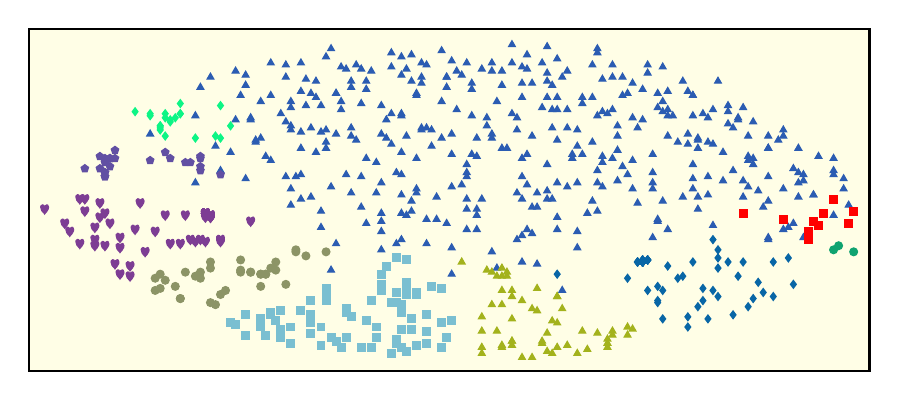
\begin{tikzpicture}[y=\textwidth/4.7,x=\textwidth/1.9, background rectangle/.style={draw=black, thick, fill=yellow!10,},show background rectangle]
\def\marRad{0.5mm}
\definecolor{color0}{rgb}{0.06,0.64,0.44}
\definecolor{color1}{rgb}{1.00,0.00,0.00}
\definecolor{color2}{rgb}{0.17,0.36,0.70}
\definecolor{color3}{rgb}{0.05,0.96,0.52}
\definecolor{color4}{rgb}{0.38,0.31,0.64}
\definecolor{color5}{rgb}{0.49,0.24,0.58}
\definecolor{color6}{rgb}{0.55,0.58,0.40}
\definecolor{color7}{rgb}{0.48,0.75,0.82}
\definecolor{color8}{rgb}{0.64,0.70,0.11}
\definecolor{color9}{rgb}{0.03,0.40,0.65}
\path[fill=color0,draw=color0,mark size=\marRad, mark=*] plot coordinates {(0.75, -0.24)};
\path[fill=color0,draw=color0,mark size=\marRad, mark=*] plot coordinates {(0.76, -0.22)};
\path[fill=color0,draw=color0,mark size=\marRad, mark=*] plot coordinates {(0.79, -0.25)};
\path[fill=color2,draw=color2,mark size=\marRad, mark=triangle*] plot coordinates {(0.19, 0.57)};
\path[fill=color2,draw=color2,mark size=\marRad, mark=triangle*] plot coordinates {(0.09, 0.26)};
\path[fill=color2,draw=color2,mark size=\marRad, mark=triangle*] plot coordinates {(0.50, 0.03)};
\path[fill=color2,draw=color2,mark size=\marRad, mark=triangle*] plot coordinates {(-0.21, 0.59)};
\path[fill=color2,draw=color2,mark size=\marRad, mark=triangle*] plot coordinates {(-0.02, 0.61)};
\path[fill=color2,draw=color2,mark size=\marRad, mark=triangle*] plot coordinates {(0.42, 0.45)};
\path[fill=color2,draw=color2,mark size=\marRad, mark=triangle*] plot coordinates {(0.03, 0.23)};
\path[fill=color2,draw=color2,mark size=\marRad, mark=triangle*] plot coordinates {(-0.11, 0.24)};
\path[fill=color2,draw=color2,mark size=\marRad, mark=triangle*] plot coordinates {(0.28, 0.09)};
\path[fill=color2,draw=color2,mark size=\marRad, mark=triangle*] plot coordinates {(-0.26, 0.35)};
\path[fill=color2,draw=color2,mark size=\marRad, mark=triangle*] plot coordinates {(-0.14, 0.31)};
\path[fill=color2,draw=color2,mark size=\marRad, mark=triangle*] plot coordinates {(0.42, 0.32)};
\path[fill=color2,draw=color2,mark size=\marRad, mark=triangle*] plot coordinates {(0.12, 0.35)};
\path[fill=color2,draw=color2,mark size=\marRad, mark=triangle*] plot coordinates {(-0.31, 0.54)};
\path[fill=color2,draw=color2,mark size=\marRad, mark=triangle*] plot coordinates {(0.44, 0.29)};
\path[fill=color2,draw=color2,mark size=\marRad, mark=triangle*] plot coordinates {(-0.18, 0.59)};
\path[fill=color2,draw=color2,mark size=\marRad, mark=triangle*] plot coordinates {(-0.34, 0.39)};
\path[fill=color2,draw=color2,mark size=\marRad, mark=triangle*] plot coordinates {(-0.21, 0.04)};
\path[fill=color2,draw=color2,mark size=\marRad, mark=triangle*] plot coordinates {(-0.40, 0.30)};
\path[fill=color2,draw=color2,mark size=\marRad, mark=triangle*] plot coordinates {(0.07, 0.33)};
\path[fill=color2,draw=color2,mark size=\marRad, mark=triangle*] plot coordinates {(-0.38, 0.22)};
\path[fill=color2,draw=color2,mark size=\marRad, mark=triangle*] plot coordinates {(0.14, 0.08)};
\path[fill=color2,draw=color2,mark size=\marRad, mark=triangle*] plot coordinates {(-0.02, 0.61)};
\path[fill=color2,draw=color2,mark size=\marRad, mark=triangle*] plot coordinates {(0.14, 0.72)};
\path[fill=color2,draw=color2,mark size=\marRad, mark=triangle*] plot coordinates {(0.51, -0.12)};
\path[fill=color2,draw=color2,mark size=\marRad, mark=triangle*] plot coordinates {(0.25, 0.48)};
\path[fill=color2,draw=color2,mark size=\marRad, mark=triangle*] plot coordinates {(0.51, 0.28)};
\path[fill=color2,draw=color2,mark size=\marRad, mark=triangle*] plot coordinates {(0.39, 0.14)};
\path[fill=color2,draw=color2,mark size=\marRad, mark=triangle*] plot coordinates {(0.54, 0.47)};
\path[fill=color2,draw=color2,mark size=\marRad, mark=triangle*] plot coordinates {(0.50, 0.29)};
\path[fill=color2,draw=color2,mark size=\marRad, mark=triangle*] plot coordinates {(0.27, 0.29)};
\path[fill=color2,draw=color2,mark size=\marRad, mark=triangle*] plot coordinates {(-0.04, 0.02)};
\path[fill=color2,draw=color2,mark size=\marRad, mark=triangle*] plot coordinates {(-0.52, 0.09)};
\path[fill=color2,draw=color2,mark size=\marRad, mark=triangle*] plot coordinates {(-0.11, 0.62)};
\path[fill=color2,draw=color2,mark size=\marRad, mark=triangle*] plot coordinates {(0.15, -0.16)};
\path[fill=color2,draw=color2,mark size=\marRad, mark=triangle*] plot coordinates {(0.67, -0.11)};
\path[fill=color2,draw=color2,mark size=\marRad, mark=triangle*] plot coordinates {(0.39, 0.23)};
\path[fill=color2,draw=color2,mark size=\marRad, mark=triangle*] plot coordinates {(-0.29, 0.53)};
\path[fill=color2,draw=color2,mark size=\marRad, mark=triangle*] plot coordinates {(0.46, 0.28)};
\path[fill=color2,draw=color2,mark size=\marRad, mark=triangle*] plot coordinates {(-0.28, 0.24)};
\path[fill=color2,draw=color2,mark size=\marRad, mark=triangle*] plot coordinates {(0.08, 0.49)};
\path[fill=color2,draw=color2,mark size=\marRad, mark=triangle*] plot coordinates {(-0.24, 0.53)};
\path[fill=color2,draw=color2,mark size=\marRad, mark=triangle*] plot coordinates {(-0.25, -0.34)};
\path[fill=color2,draw=color2,mark size=\marRad, mark=triangle*] plot coordinates {(0.21, -0.44)};
\path[fill=color2,draw=color2,mark size=\marRad, mark=triangle*] plot coordinates {(-0.33, 0.06)};
\path[fill=color2,draw=color2,mark size=\marRad, mark=triangle*] plot coordinates {(0.42, 0.42)};
\path[fill=color2,draw=color2,mark size=\marRad, mark=triangle*] plot coordinates {(-0.07, 0.61)};
\path[fill=color2,draw=color2,mark size=\marRad, mark=triangle*] plot coordinates {(0.10, 0.26)};
\path[fill=color2,draw=color2,mark size=\marRad, mark=triangle*] plot coordinates {(-0.11, 0.43)};
\path[fill=color2,draw=color2,mark size=\marRad, mark=triangle*] plot coordinates {(0.13, 0.01)};
\path[fill=color2,draw=color2,mark size=\marRad, mark=triangle*] plot coordinates {(-0.51, 0.56)};
\path[fill=color2,draw=color2,mark size=\marRad, mark=triangle*] plot coordinates {(0.33, 0.52)};
\path[fill=color2,draw=color2,mark size=\marRad, mark=triangle*] plot coordinates {(-0.28, 0.51)};
\path[fill=color2,draw=color2,mark size=\marRad, mark=triangle*] plot coordinates {(-0.06, 0.67)};
\path[fill=color2,draw=color2,mark size=\marRad, mark=triangle*] plot coordinates {(0.67, 0.16)};
\path[fill=color2,draw=color2,mark size=\marRad, mark=triangle*] plot coordinates {(-0.09, -0.00)};
\path[fill=color2,draw=color2,mark size=\marRad, mark=triangle*] plot coordinates {(-0.26, 0.29)};
\path[fill=color2,draw=color2,mark size=\marRad, mark=triangle*] plot coordinates {(0.65, 0.06)};
\path[fill=color2,draw=color2,mark size=\marRad, mark=triangle*] plot coordinates {(0.45, 0.02)};
\path[fill=color2,draw=color2,mark size=\marRad, mark=triangle*] plot coordinates {(0.27, 0.00)};
\path[fill=color2,draw=color2,mark size=\marRad, mark=triangle*] plot coordinates {(-0.19, 0.12)};
\path[fill=color2,draw=color2,mark size=\marRad, mark=triangle*] plot coordinates {(0.07, 0.64)};
\path[fill=color2,draw=color2,mark size=\marRad, mark=triangle*] plot coordinates {(-0.08, 0.53)};
\path[fill=color2,draw=color2,mark size=\marRad, mark=triangle*] plot coordinates {(-0.14, 0.40)};
\path[fill=color2,draw=color2,mark size=\marRad, mark=triangle*] plot coordinates {(0.62, 0.26)};
\path[fill=color2,draw=color2,mark size=\marRad, mark=triangle*] plot coordinates {(0.55, 0.36)};
\path[fill=color2,draw=color2,mark size=\marRad, mark=triangle*] plot coordinates {(0.11, 0.43)};
\path[fill=color2,draw=color2,mark size=\marRad, mark=triangle*] plot coordinates {(0.16, -0.03)};
\path[fill=color2,draw=color2,mark size=\marRad, mark=triangle*] plot coordinates {(0.41, 0.44)};
\path[fill=color2,draw=color2,mark size=\marRad, mark=triangle*] plot coordinates {(-0.07, 0.36)};
\path[fill=color2,draw=color2,mark size=\marRad, mark=triangle*] plot coordinates {(-0.25, 0.07)};
\path[fill=color2,draw=color2,mark size=\marRad, mark=triangle*] plot coordinates {(0.68, 0.14)};
\path[fill=color2,draw=color2,mark size=\marRad, mark=triangle*] plot coordinates {(0.11, 0.68)};
\path[fill=color2,draw=color2,mark size=\marRad, mark=triangle*] plot coordinates {(0.15, 0.32)};
\path[fill=color2,draw=color2,mark size=\marRad, mark=triangle*] plot coordinates {(-0.11, 0.03)};
\path[fill=color2,draw=color2,mark size=\marRad, mark=triangle*] plot coordinates {(-0.48, 0.27)};
\path[fill=color2,draw=color2,mark size=\marRad, mark=triangle*] plot coordinates {(0.51, 0.45)};
\path[fill=color2,draw=color2,mark size=\marRad, mark=triangle*] plot coordinates {(0.32, 0.37)};
\path[fill=color2,draw=color2,mark size=\marRad, mark=triangle*] plot coordinates {(-0.43, 0.52)};
\path[fill=color2,draw=color2,mark size=\marRad, mark=triangle*] plot coordinates {(0.48, 0.26)};
\path[fill=color2,draw=color2,mark size=\marRad, mark=triangle*] plot coordinates {(0.04, 0.31)};
\path[fill=color2,draw=color2,mark size=\marRad, mark=triangle*] plot coordinates {(0.58, 0.22)};
\path[fill=color2,draw=color2,mark size=\marRad, mark=triangle*] plot coordinates {(0.69, -0.18)};
\path[fill=color2,draw=color2,mark size=\marRad, mark=triangle*] plot coordinates {(-0.11, 0.42)};
\path[fill=color2,draw=color2,mark size=\marRad, mark=triangle*] plot coordinates {(0.23, 0.23)};
\path[fill=color2,draw=color2,mark size=\marRad, mark=triangle*] plot coordinates {(0.24, -0.23)};
\path[fill=color2,draw=color2,mark size=\marRad, mark=triangle*] plot coordinates {(0.28, 0.15)};
\path[fill=color2,draw=color2,mark size=\marRad, mark=triangle*] plot coordinates {(0.18, 0.76)};
\path[fill=color2,draw=color2,mark size=\marRad, mark=triangle*] plot coordinates {(0.00, 0.45)};
\path[fill=color2,draw=color2,mark size=\marRad, mark=triangle*] plot coordinates {(-0.10, 0.65)};
\path[fill=color2,draw=color2,mark size=\marRad, mark=triangle*] plot coordinates {(0.20, 0.51)};
\path[fill=color2,draw=color2,mark size=\marRad, mark=triangle*] plot coordinates {(0.46, 0.33)};
\path[fill=color2,draw=color2,mark size=\marRad, mark=triangle*] plot coordinates {(-0.30, 0.47)};
\path[fill=color2,draw=color2,mark size=\marRad, mark=triangle*] plot coordinates {(0.23, 0.21)};
\path[fill=color2,draw=color2,mark size=\marRad, mark=triangle*] plot coordinates {(0.68, 0.02)};
\path[fill=color2,draw=color2,mark size=\marRad, mark=triangle*] plot coordinates {(0.15, -0.03)};
\path[fill=color2,draw=color2,mark size=\marRad, mark=triangle*] plot coordinates {(-0.10, -0.07)};
\path[fill=color2,draw=color2,mark size=\marRad, mark=triangle*] plot coordinates {(0.40, 0.53)};
\path[fill=color2,draw=color2,mark size=\marRad, mark=triangle*] plot coordinates {(0.53, 0.10)};
\path[fill=color2,draw=color2,mark size=\marRad, mark=triangle*] plot coordinates {(-0.45, 0.24)};
\path[fill=color2,draw=color2,mark size=\marRad, mark=triangle*] plot coordinates {(0.31, 0.61)};
\path[fill=color2,draw=color2,mark size=\marRad, mark=triangle*] plot coordinates {(0.25, 0.23)};
\path[fill=color2,draw=color2,mark size=\marRad, mark=triangle*] plot coordinates {(-0.26, 0.71)};
\path[fill=color2,draw=color2,mark size=\marRad, mark=triangle*] plot coordinates {(0.62, -0.00)};
\path[fill=color2,draw=color2,mark size=\marRad, mark=triangle*] plot coordinates {(0.02, 0.18)};
\path[fill=color2,draw=color2,mark size=\marRad, mark=triangle*] plot coordinates {(0.07, -0.25)};
\path[fill=color2,draw=color2,mark size=\marRad, mark=triangle*] plot coordinates {(-0.31, 0.34)};
\path[fill=color2,draw=color2,mark size=\marRad, mark=triangle*] plot coordinates {(0.58, 0.07)};
\path[fill=color2,draw=color2,mark size=\marRad, mark=triangle*] plot coordinates {(0.02, -0.14)};
\path[fill=color2,draw=color2,mark size=\marRad, mark=triangle*] plot coordinates {(0.55, 0.15)};
\path[fill=color2,draw=color2,mark size=\marRad, mark=triangle*] plot coordinates {(0.13, -0.17)};
\path[fill=color2,draw=color2,mark size=\marRad, mark=triangle*] plot coordinates {(0.48, 0.31)};
\path[fill=color2,draw=color2,mark size=\marRad, mark=triangle*] plot coordinates {(0.48, -0.04)};
\path[fill=color2,draw=color2,mark size=\marRad, mark=triangle*] plot coordinates {(0.04, -0.04)};
\path[fill=color2,draw=color2,mark size=\marRad, mark=triangle*] plot coordinates {(-0.06, -0.09)};
\path[fill=color2,draw=color2,mark size=\marRad, mark=triangle*] plot coordinates {(-0.18, 0.21)};
\path[fill=color2,draw=color2,mark size=\marRad, mark=triangle*] plot coordinates {(-0.13, 0.73)};
\path[fill=color2,draw=color2,mark size=\marRad, mark=triangle*] plot coordinates {(0.03, 0.42)};
\path[fill=color2,draw=color2,mark size=\marRad, mark=triangle*] plot coordinates {(0.50, 0.41)};
\path[fill=color2,draw=color2,mark size=\marRad, mark=triangle*] plot coordinates {(0.28, -0.05)};
\path[fill=color2,draw=color2,mark size=\marRad, mark=triangle*] plot coordinates {(0.49, 0.43)};
\path[fill=color2,draw=color2,mark size=\marRad, mark=triangle*] plot coordinates {(0.59, 0.18)};
\path[fill=color2,draw=color2,mark size=\marRad, mark=triangle*] plot coordinates {(-0.23, 0.66)};
\path[fill=color2,draw=color2,mark size=\marRad, mark=triangle*] plot coordinates {(0.14, 0.23)};
\path[fill=color2,draw=color2,mark size=\marRad, mark=triangle*] plot coordinates {(0.21, 0.61)};
\path[fill=color2,draw=color2,mark size=\marRad, mark=triangle*] plot coordinates {(0.27, 0.51)};
\path[fill=color2,draw=color2,mark size=\marRad, mark=triangle*] plot coordinates {(-0.39, 0.49)};
\path[fill=color2,draw=color2,mark size=\marRad, mark=triangle*] plot coordinates {(0.34, 0.53)};
\path[fill=color2,draw=color2,mark size=\marRad, mark=triangle*] plot coordinates {(0.32, 0.25)};
\path[fill=color2,draw=color2,mark size=\marRad, mark=triangle*] plot coordinates {(-0.31, 0.26)};
\path[fill=color2,draw=color2,mark size=\marRad, mark=triangle*] plot coordinates {(-0.19, 0.48)};
\path[fill=color2,draw=color2,mark size=\marRad, mark=triangle*] plot coordinates {(0.19, 0.01)};
\path[fill=color2,draw=color2,mark size=\marRad, mark=triangle*] plot coordinates {(0.20, 0.30)};
\path[fill=color2,draw=color2,mark size=\marRad, mark=triangle*] plot coordinates {(0.18, 0.51)};
\path[fill=color2,draw=color2,mark size=\marRad, mark=triangle*] plot coordinates {(-0.21, 0.32)};
\path[fill=color2,draw=color2,mark size=\marRad, mark=triangle*] plot coordinates {(-0.39, 0.31)};
\path[fill=color2,draw=color2,mark size=\marRad, mark=triangle*] plot coordinates {(0.59, 0.21)};
\path[fill=color2,draw=color2,mark size=\marRad, mark=triangle*] plot coordinates {(0.48, 0.30)};
\path[fill=color2,draw=color2,mark size=\marRad, mark=triangle*] plot coordinates {(0.40, -0.10)};
\path[fill=color2,draw=color2,mark size=\marRad, mark=triangle*] plot coordinates {(-0.33, -0.02)};
\path[fill=color2,draw=color2,mark size=\marRad, mark=triangle*] plot coordinates {(-0.03, 0.31)};
\path[fill=color2,draw=color2,mark size=\marRad, mark=triangle*] plot coordinates {(-0.08, 0.21)};
\path[fill=color2,draw=color2,mark size=\marRad, mark=triangle*] plot coordinates {(0.65, 0.32)};
\path[fill=color2,draw=color2,mark size=\marRad, mark=triangle*] plot coordinates {(0.29, 0.22)};
\path[fill=color2,draw=color2,mark size=\marRad, mark=triangle*] plot coordinates {(0.13, 0.66)};
\path[fill=color2,draw=color2,mark size=\marRad, mark=triangle*] plot coordinates {(0.42, 0.54)};
\path[fill=color2,draw=color2,mark size=\marRad, mark=triangle*] plot coordinates {(-0.44, 0.40)};
\path[fill=color2,draw=color2,mark size=\marRad, mark=triangle*] plot coordinates {(-0.13, 0.66)};
\path[fill=color2,draw=color2,mark size=\marRad, mark=triangle*] plot coordinates {(0.47, 0.11)};
\path[fill=color2,draw=color2,mark size=\marRad, mark=triangle*] plot coordinates {(-0.20, 0.30)};
\path[fill=color2,draw=color2,mark size=\marRad, mark=triangle*] plot coordinates {(-0.11, 0.71)};
\path[fill=color2,draw=color2,mark size=\marRad, mark=triangle*] plot coordinates {(0.22, 0.07)};
\path[fill=color2,draw=color2,mark size=\marRad, mark=triangle*] plot coordinates {(-0.19, 0.65)};
\path[fill=color2,draw=color2,mark size=\marRad, mark=triangle*] plot coordinates {(0.33, 0.17)};
\path[fill=color2,draw=color2,mark size=\marRad, mark=triangle*] plot coordinates {(0.72, 0.22)};
\path[fill=color2,draw=color2,mark size=\marRad, mark=triangle*] plot coordinates {(-0.28, 0.59)};
\path[fill=color2,draw=color2,mark size=\marRad, mark=triangle*] plot coordinates {(-0.27, -0.05)};
\path[fill=color2,draw=color2,mark size=\marRad, mark=triangle*] plot coordinates {(0.13, 0.51)};
\path[fill=color2,draw=color2,mark size=\marRad, mark=triangle*] plot coordinates {(0.38, 0.63)};
\path[fill=color2,draw=color2,mark size=\marRad, mark=triangle*] plot coordinates {(0.34, 0.13)};
\path[fill=color2,draw=color2,mark size=\marRad, mark=triangle*] plot coordinates {(0.65, 0.35)};
\path[fill=color2,draw=color2,mark size=\marRad, mark=triangle*] plot coordinates {(0.09, 0.57)};
\path[fill=color2,draw=color2,mark size=\marRad, mark=triangle*] plot coordinates {(-0.16, 0.04)};
\path[fill=color2,draw=color2,mark size=\marRad, mark=triangle*] plot coordinates {(0.20, 0.45)};
\path[fill=color2,draw=color2,mark size=\marRad, mark=triangle*] plot coordinates {(-0.00, 0.64)};
\path[fill=color2,draw=color2,mark size=\marRad, mark=triangle*] plot coordinates {(-0.01, 0.33)};
\path[fill=color2,draw=color2,mark size=\marRad, mark=triangle*] plot coordinates {(-0.09, -0.05)};
\path[fill=color2,draw=color2,mark size=\marRad, mark=triangle*] plot coordinates {(0.36, 0.36)};
\path[fill=color2,draw=color2,mark size=\marRad, mark=triangle*] plot coordinates {(0.68, 0.09)};
\path[fill=color2,draw=color2,mark size=\marRad, mark=triangle*] plot coordinates {(0.41, 0.49)};
\path[fill=color2,draw=color2,mark size=\marRad, mark=triangle*] plot coordinates {(0.02, 0.14)};
\path[fill=color2,draw=color2,mark size=\marRad, mark=triangle*] plot coordinates {(0.47, 0.06)};
\path[fill=color2,draw=color2,mark size=\marRad, mark=triangle*] plot coordinates {(-0.31, 0.13)};
\path[fill=color2,draw=color2,mark size=\marRad, mark=triangle*] plot coordinates {(0.47, 0.52)};
\path[fill=color2,draw=color2,mark size=\marRad, mark=triangle*] plot coordinates {(0.56, 0.41)};
\path[fill=color2,draw=color2,mark size=\marRad, mark=triangle*] plot coordinates {(0.03, 0.55)};
\path[fill=color2,draw=color2,mark size=\marRad, mark=triangle*] plot coordinates {(-0.24, -0.21)};
\path[fill=color2,draw=color2,mark size=\marRad, mark=triangle*] plot coordinates {(0.75, -0.07)};
\path[fill=color2,draw=color2,mark size=\marRad, mark=triangle*] plot coordinates {(0.61, -0.03)};
\path[fill=color2,draw=color2,mark size=\marRad, mark=triangle*] plot coordinates {(0.27, 0.67)};
\path[fill=color2,draw=color2,mark size=\marRad, mark=triangle*] plot coordinates {(-0.13, 0.43)};
\path[fill=color2,draw=color2,mark size=\marRad, mark=triangle*] plot coordinates {(0.02, 0.01)};
\path[fill=color2,draw=color2,mark size=\marRad, mark=triangle*] plot coordinates {(-0.24, 0.33)};
\path[fill=color2,draw=color2,mark size=\marRad, mark=triangle*] plot coordinates {(0.25, 0.51)};
\path[fill=color2,draw=color2,mark size=\marRad, mark=triangle*] plot coordinates {(0.12, 0.04)};
\path[fill=color2,draw=color2,mark size=\marRad, mark=triangle*] plot coordinates {(0.28, 0.75)};
\path[fill=color2,draw=color2,mark size=\marRad, mark=triangle*] plot coordinates {(0.71, 0.03)};
\path[fill=color2,draw=color2,mark size=\marRad, mark=triangle*] plot coordinates {(0.06, 0.41)};
\path[fill=color2,draw=color2,mark size=\marRad, mark=triangle*] plot coordinates {(0.40, -0.09)};
\path[fill=color2,draw=color2,mark size=\marRad, mark=triangle*] plot coordinates {(0.60, 0.05)};
\path[fill=color2,draw=color2,mark size=\marRad, mark=triangle*] plot coordinates {(0.14, 0.65)};
\path[fill=color2,draw=color2,mark size=\marRad, mark=triangle*] plot coordinates {(-0.07, 0.68)};
\path[fill=color2,draw=color2,mark size=\marRad, mark=triangle*] plot coordinates {(0.69, 0.10)};
\path[fill=color2,draw=color2,mark size=\marRad, mark=triangle*] plot coordinates {(-0.32, 0.12)};
\path[fill=color2,draw=color2,mark size=\marRad, mark=triangle*] plot coordinates {(-0.17, 0.64)};
\path[fill=color2,draw=color2,mark size=\marRad, mark=triangle*] plot coordinates {(0.01, 0.62)};
\path[fill=color2,draw=color2,mark size=\marRad, mark=triangle*] plot coordinates {(0.22, 0.45)};
\path[fill=color2,draw=color2,mark size=\marRad, mark=triangle*] plot coordinates {(-0.42, 0.57)};
\path[fill=color2,draw=color2,mark size=\marRad, mark=triangle*] plot coordinates {(-0.33, 0.35)};
\path[fill=color2,draw=color2,mark size=\marRad, mark=triangle*] plot coordinates {(0.24, 0.09)};
\path[fill=color2,draw=color2,mark size=\marRad, mark=triangle*] plot coordinates {(0.65, -0.14)};
\path[fill=color2,draw=color2,mark size=\marRad, mark=triangle*] plot coordinates {(0.28, 0.42)};
\path[fill=color2,draw=color2,mark size=\marRad, mark=triangle*] plot coordinates {(-0.27, 0.34)};
\path[fill=color2,draw=color2,mark size=\marRad, mark=triangle*] plot coordinates {(-0.23, 0.49)};
\path[fill=color2,draw=color2,mark size=\marRad, mark=triangle*] plot coordinates {(-0.18, -0.11)};
\path[fill=color2,draw=color2,mark size=\marRad, mark=triangle*] plot coordinates {(0.22, 0.36)};
\path[fill=color2,draw=color2,mark size=\marRad, mark=triangle*] plot coordinates {(-0.29, 0.02)};
\path[fill=color2,draw=color2,mark size=\marRad, mark=triangle*] plot coordinates {(-0.29, 0.36)};
\path[fill=color2,draw=color2,mark size=\marRad, mark=triangle*] plot coordinates {(-0.24, 0.53)};
\path[fill=color2,draw=color2,mark size=\marRad, mark=triangle*] plot coordinates {(0.75, 0.13)};
\path[fill=color2,draw=color2,mark size=\marRad, mark=triangle*] plot coordinates {(0.52, 0.59)};
\path[fill=color2,draw=color2,mark size=\marRad, mark=triangle*] plot coordinates {(-0.23, 0.45)};
\path[fill=color2,draw=color2,mark size=\marRad, mark=triangle*] plot coordinates {(0.39, 0.06)};
\path[fill=color2,draw=color2,mark size=\marRad, mark=triangle*] plot coordinates {(0.19, 0.45)};
\path[fill=color2,draw=color2,mark size=\marRad, mark=triangle*] plot coordinates {(0.37, 0.55)};
\path[fill=color2,draw=color2,mark size=\marRad, mark=triangle*] plot coordinates {(-0.13, 0.28)};
\path[fill=color2,draw=color2,mark size=\marRad, mark=triangle*] plot coordinates {(-0.01, 0.69)};
\path[fill=color2,draw=color2,mark size=\marRad, mark=triangle*] plot coordinates {(0.30, 0.43)};
\path[fill=color2,draw=color2,mark size=\marRad, mark=triangle*] plot coordinates {(0.22, 0.64)};
\path[fill=color2,draw=color2,mark size=\marRad, mark=triangle*] plot coordinates {(0.20, -0.08)};
\path[fill=color2,draw=color2,mark size=\marRad, mark=triangle*] plot coordinates {(0.29, 0.60)};
\path[fill=color2,draw=color2,mark size=\marRad, mark=triangle*] plot coordinates {(-0.21, 0.56)};
\path[fill=color2,draw=color2,mark size=\marRad, mark=triangle*] plot coordinates {(-0.06, -0.21)};
\path[fill=color2,draw=color2,mark size=\marRad, mark=triangle*] plot coordinates {(0.04, -0.07)};
\path[fill=color2,draw=color2,mark size=\marRad, mark=triangle*] plot coordinates {(-0.08, 0.06)};
\path[fill=color2,draw=color2,mark size=\marRad, mark=triangle*] plot coordinates {(0.18, 0.18)};
\path[fill=color2,draw=color2,mark size=\marRad, mark=triangle*] plot coordinates {(-0.15, -0.24)};
\path[fill=color2,draw=color2,mark size=\marRad, mark=triangle*] plot coordinates {(0.54, 0.44)};
\path[fill=color2,draw=color2,mark size=\marRad, mark=triangle*] plot coordinates {(0.68, 0.26)};
\path[fill=color2,draw=color2,mark size=\marRad, mark=triangle*] plot coordinates {(0.57, 0.02)};
\path[fill=color2,draw=color2,mark size=\marRad, mark=triangle*] plot coordinates {(0.02, -0.04)};
\path[fill=color2,draw=color2,mark size=\marRad, mark=triangle*] plot coordinates {(-0.02, 0.56)};
\path[fill=color2,draw=color2,mark size=\marRad, mark=triangle*] plot coordinates {(-0.34, 0.61)};
\path[fill=color2,draw=color2,mark size=\marRad, mark=triangle*] plot coordinates {(0.18, 0.63)};
\path[fill=color2,draw=color2,mark size=\marRad, mark=triangle*] plot coordinates {(0.53, 0.24)};
\path[fill=color2,draw=color2,mark size=\marRad, mark=triangle*] plot coordinates {(0.07, 0.68)};
\path[fill=color2,draw=color2,mark size=\marRad, mark=triangle*] plot coordinates {(-0.37, 0.20)};
\path[fill=color2,draw=color2,mark size=\marRad, mark=triangle*] plot coordinates {(0.71, 0.03)};
\path[fill=color2,draw=color2,mark size=\marRad, mark=triangle*] plot coordinates {(0.35, 0.06)};
\path[fill=color2,draw=color2,mark size=\marRad, mark=triangle*] plot coordinates {(0.47, 0.52)};
\path[fill=color2,draw=color2,mark size=\marRad, mark=triangle*] plot coordinates {(0.38, 0.67)};
\path[fill=color2,draw=color2,mark size=\marRad, mark=triangle*] plot coordinates {(0.65, -0.10)};
\path[fill=color2,draw=color2,mark size=\marRad, mark=triangle*] plot coordinates {(0.57, 0.46)};
\path[fill=color2,draw=color2,mark size=\marRad, mark=triangle*] plot coordinates {(0.29, 0.07)};
\path[fill=color2,draw=color2,mark size=\marRad, mark=triangle*] plot coordinates {(-0.18, 0.55)};
\path[fill=color2,draw=color2,mark size=\marRad, mark=triangle*] plot coordinates {(0.13, 0.12)};
\path[fill=color2,draw=color2,mark size=\marRad, mark=triangle*] plot coordinates {(-0.10, 0.32)};
\path[fill=color2,draw=color2,mark size=\marRad, mark=triangle*] plot coordinates {(-0.42, 0.62)};
\path[fill=color2,draw=color2,mark size=\marRad, mark=triangle*] plot coordinates {(-0.15, -0.06)};
\path[fill=color2,draw=color2,mark size=\marRad, mark=triangle*] plot coordinates {(-0.19, -0.03)};
\path[fill=color2,draw=color2,mark size=\marRad, mark=triangle*] plot coordinates {(-0.34, 0.12)};
\path[fill=color2,draw=color2,mark size=\marRad, mark=triangle*] plot coordinates {(0.20, 0.09)};
\path[fill=color2,draw=color2,mark size=\marRad, mark=triangle*] plot coordinates {(0.41, 0.00)};
\path[fill=color2,draw=color2,mark size=\marRad, mark=triangle*] plot coordinates {(0.36, -0.01)};
\path[fill=color2,draw=color2,mark size=\marRad, mark=triangle*] plot coordinates {(-0.08, 0.52)};
\path[fill=color2,draw=color2,mark size=\marRad, mark=triangle*] plot coordinates {(0.09, 0.64)};
\path[fill=color2,draw=color2,mark size=\marRad, mark=triangle*] plot coordinates {(0.32, 0.10)};
\path[fill=color2,draw=color2,mark size=\marRad, mark=triangle*] plot coordinates {(0.47, 0.42)};
\path[fill=color2,draw=color2,mark size=\marRad, mark=triangle*] plot coordinates {(-0.01, 0.07)};
\path[fill=color2,draw=color2,mark size=\marRad, mark=triangle*] plot coordinates {(-0.31, 0.01)};
\path[fill=color2,draw=color2,mark size=\marRad, mark=triangle*] plot coordinates {(-0.21, 0.36)};
\path[fill=color2,draw=color2,mark size=\marRad, mark=triangle*] plot coordinates {(-0.22, 0.13)};
\path[fill=color2,draw=color2,mark size=\marRad, mark=triangle*] plot coordinates {(-0.44, 0.64)};
\path[fill=color2,draw=color2,mark size=\marRad, mark=triangle*] plot coordinates {(-0.33, 0.46)};
\path[fill=color2,draw=color2,mark size=\marRad, mark=triangle*] plot coordinates {(0.02, 0.12)};
\path[fill=color2,draw=color2,mark size=\marRad, mark=triangle*] plot coordinates {(0.06, 0.37)};
\path[fill=color2,draw=color2,mark size=\marRad, mark=triangle*] plot coordinates {(-0.03, 0.74)};
\path[fill=color2,draw=color2,mark size=\marRad, mark=triangle*] plot coordinates {(-0.35, 0.43)};
\path[fill=color2,draw=color2,mark size=\marRad, mark=triangle*] plot coordinates {(0.75, 0.21)};
\path[fill=color2,draw=color2,mark size=\marRad, mark=triangle*] plot coordinates {(0.39, 0.09)};
\path[fill=color2,draw=color2,mark size=\marRad, mark=triangle*] plot coordinates {(0.12, 0.41)};
\path[fill=color2,draw=color2,mark size=\marRad, mark=triangle*] plot coordinates {(0.40, 0.46)};
\path[fill=color2,draw=color2,mark size=\marRad, mark=triangle*] plot coordinates {(0.18, 0.05)};
\path[fill=color2,draw=color2,mark size=\marRad, mark=triangle*] plot coordinates {(-0.49, 0.61)};
\path[fill=color2,draw=color2,mark size=\marRad, mark=triangle*] plot coordinates {(-0.15, 0.33)};
\path[fill=color2,draw=color2,mark size=\marRad, mark=triangle*] plot coordinates {(0.58, 0.32)};
\path[fill=color2,draw=color2,mark size=\marRad, mark=triangle*] plot coordinates {(0.35, 0.41)};
\path[fill=color2,draw=color2,mark size=\marRad, mark=triangle*] plot coordinates {(0.16, 0.04)};
\path[fill=color2,draw=color2,mark size=\marRad, mark=triangle*] plot coordinates {(-0.11, 0.13)};
\path[fill=color2,draw=color2,mark size=\marRad, mark=triangle*] plot coordinates {(-0.01, -0.23)};
\path[fill=color2,draw=color2,mark size=\marRad, mark=triangle*] plot coordinates {(0.04, 0.22)};
\path[fill=color2,draw=color2,mark size=\marRad, mark=triangle*] plot coordinates {(0.77, 0.11)};
\path[fill=color2,draw=color2,mark size=\marRad, mark=triangle*] plot coordinates {(-0.01, 0.23)};
\path[fill=color2,draw=color2,mark size=\marRad, mark=triangle*] plot coordinates {(-0.15, -0.15)};
\path[fill=color2,draw=color2,mark size=\marRad, mark=triangle*] plot coordinates {(0.17, 0.68)};
\path[fill=color2,draw=color2,mark size=\marRad, mark=triangle*] plot coordinates {(-0.12, -0.21)};
\path[fill=color2,draw=color2,mark size=\marRad, mark=triangle*] plot coordinates {(0.24, 0.35)};
\path[fill=color2,draw=color2,mark size=\marRad, mark=triangle*] plot coordinates {(-0.33, 0.49)};
\path[fill=color2,draw=color2,mark size=\marRad, mark=triangle*] plot coordinates {(0.13, 0.21)};
\path[fill=color2,draw=color2,mark size=\marRad, mark=triangle*] plot coordinates {(0.08, -0.33)};
\path[fill=color2,draw=color2,mark size=\marRad, mark=triangle*] plot coordinates {(0.62, 0.26)};
\path[fill=color2,draw=color2,mark size=\marRad, mark=triangle*] plot coordinates {(0.28, 0.73)};
\path[fill=color2,draw=color2,mark size=\marRad, mark=triangle*] plot coordinates {(-0.15, -0.10)};
\path[fill=color2,draw=color2,mark size=\marRad, mark=triangle*] plot coordinates {(-0.12, 0.14)};
\path[fill=color2,draw=color2,mark size=\marRad, mark=triangle*] plot coordinates {(0.20, 0.70)};
\path[fill=color2,draw=color2,mark size=\marRad, mark=triangle*] plot coordinates {(0.41, 0.66)};
\path[fill=color2,draw=color2,mark size=\marRad, mark=triangle*] plot coordinates {(-0.34, 0.67)};
\path[fill=color2,draw=color2,mark size=\marRad, mark=triangle*] plot coordinates {(-0.27, -0.13)};
\path[fill=color2,draw=color2,mark size=\marRad, mark=triangle*] plot coordinates {(0.64, 0.30)};
\path[fill=color2,draw=color2,mark size=\marRad, mark=triangle*] plot coordinates {(-0.02, -0.11)};
\path[fill=color2,draw=color2,mark size=\marRad, mark=triangle*] plot coordinates {(-0.06, 0.36)};
\path[fill=color2,draw=color2,mark size=\marRad, mark=triangle*] plot coordinates {(0.20, -0.14)};
\path[fill=color2,draw=color2,mark size=\marRad, mark=triangle*] plot coordinates {(-0.09, 0.72)};
\path[fill=color2,draw=color2,mark size=\marRad, mark=triangle*] plot coordinates {(0.45, 0.59)};
\path[fill=color2,draw=color2,mark size=\marRad, mark=triangle*] plot coordinates {(0.62, -0.18)};
\path[fill=color2,draw=color2,mark size=\marRad, mark=triangle*] plot coordinates {(0.77, 0.06)};
\path[fill=color2,draw=color2,mark size=\marRad, mark=triangle*] plot coordinates {(0.31, 0.21)};
\path[fill=color2,draw=color2,mark size=\marRad, mark=triangle*] plot coordinates {(0.13, 0.58)};
\path[fill=color2,draw=color2,mark size=\marRad, mark=triangle*] plot coordinates {(0.29, 0.44)};
\path[fill=color2,draw=color2,mark size=\marRad, mark=triangle*] plot coordinates {(0.07, 0.31)};
\path[fill=color2,draw=color2,mark size=\marRad, mark=triangle*] plot coordinates {(-0.33, 0.37)};
\path[fill=color2,draw=color2,mark size=\marRad, mark=triangle*] plot coordinates {(0.18, 0.59)};
\path[fill=color2,draw=color2,mark size=\marRad, mark=triangle*] plot coordinates {(0.13, -0.30)};
\path[fill=color2,draw=color2,mark size=\marRad, mark=triangle*] plot coordinates {(-0.15, 0.09)};
\path[fill=color2,draw=color2,mark size=\marRad, mark=triangle*] plot coordinates {(0.59, 0.39)};
\path[fill=color2,draw=color2,mark size=\marRad, mark=triangle*] plot coordinates {(0.05, 0.01)};
\path[fill=color2,draw=color2,mark size=\marRad, mark=triangle*] plot coordinates {(-0.09, 0.59)};
\path[fill=color2,draw=color2,mark size=\marRad, mark=triangle*] plot coordinates {(-0.31, 0.68)};
\path[fill=color2,draw=color2,mark size=\marRad, mark=triangle*] plot coordinates {(0.62, 0.32)};
\path[fill=color2,draw=color2,mark size=\marRad, mark=triangle*] plot coordinates {(0.62, 0.12)};
\path[fill=color2,draw=color2,mark size=\marRad, mark=triangle*] plot coordinates {(0.54, 0.38)};
\path[fill=color2,draw=color2,mark size=\marRad, mark=triangle*] plot coordinates {(0.24, 0.27)};
\path[fill=color2,draw=color2,mark size=\marRad, mark=triangle*] plot coordinates {(0.01, 0.08)};
\path[fill=color2,draw=color2,mark size=\marRad, mark=triangle*] plot coordinates {(-0.30, 0.60)};
\path[fill=color2,draw=color2,mark size=\marRad, mark=triangle*] plot coordinates {(0.37, 0.40)};
\path[fill=color2,draw=color2,mark size=\marRad, mark=triangle*] plot coordinates {(0.32, 0.32)};
\path[fill=color2,draw=color2,mark size=\marRad, mark=triangle*] plot coordinates {(-0.27, 0.47)};
\path[fill=color2,draw=color2,mark size=\marRad, mark=triangle*] plot coordinates {(-0.22, 0.65)};
\path[fill=color2,draw=color2,mark size=\marRad, mark=triangle*] plot coordinates {(0.05, 0.65)};
\path[fill=color2,draw=color2,mark size=\marRad, mark=triangle*] plot coordinates {(-0.16, 0.19)};
\path[fill=color2,draw=color2,mark size=\marRad, mark=triangle*] plot coordinates {(0.24, -0.15)};
\path[fill=color2,draw=color2,mark size=\marRad, mark=triangle*] plot coordinates {(-0.42, 0.11)};
\path[fill=color2,draw=color2,mark size=\marRad, mark=triangle*] plot coordinates {(-0.11, -0.06)};
\path[fill=color2,draw=color2,mark size=\marRad, mark=triangle*] plot coordinates {(-0.37, 0.68)};
\path[fill=color2,draw=color2,mark size=\marRad, mark=triangle*] plot coordinates {(0.35, 0.20)};
\path[fill=color2,draw=color2,mark size=\marRad, mark=triangle*] plot coordinates {(-0.61, 0.33)};
\path[fill=color2,draw=color2,mark size=\marRad, mark=triangle*] plot coordinates {(0.39, -0.18)};
\path[fill=color2,draw=color2,mark size=\marRad, mark=triangle*] plot coordinates {(-0.08, 0.04)};
\path[fill=color2,draw=color2,mark size=\marRad, mark=triangle*] plot coordinates {(0.33, 0.61)};
\path[fill=color2,draw=color2,mark size=\marRad, mark=triangle*] plot coordinates {(0.69, 0.13)};
\path[fill=color2,draw=color2,mark size=\marRad, mark=triangle*] plot coordinates {(0.47, 0.18)};
\path[fill=color2,draw=color2,mark size=\marRad, mark=triangle*] plot coordinates {(-0.26, 0.26)};
\path[fill=color2,draw=color2,mark size=\marRad, mark=triangle*] plot coordinates {(0.43, 0.42)};
\path[fill=color2,draw=color2,mark size=\marRad, mark=triangle*] plot coordinates {(-0.15, 0.47)};
\path[fill=color2,draw=color2,mark size=\marRad, mark=triangle*] plot coordinates {(-0.03, 0.49)};
\path[fill=color2,draw=color2,mark size=\marRad, mark=triangle*] plot coordinates {(0.18, 0.01)};
\path[fill=color2,draw=color2,mark size=\marRad, mark=triangle*] plot coordinates {(0.66, -0.13)};
\path[fill=color2,draw=color2,mark size=\marRad, mark=triangle*] plot coordinates {(0.26, -0.06)};
\path[fill=color2,draw=color2,mark size=\marRad, mark=triangle*] plot coordinates {(-0.41, 0.40)};
\path[fill=color2,draw=color2,mark size=\marRad, mark=triangle*] plot coordinates {(0.02, 0.68)};
\path[fill=color2,draw=color2,mark size=\marRad, mark=triangle*] plot coordinates {(0.35, 0.58)};
\path[fill=color2,draw=color2,mark size=\marRad, mark=triangle*] plot coordinates {(-0.01, -0.36)};
\path[fill=color2,draw=color2,mark size=\marRad, mark=triangle*] plot coordinates {(0.29, 0.19)};
\path[fill=color2,draw=color2,mark size=\marRad, mark=triangle*] plot coordinates {(-0.52, 0.42)};
\path[fill=color2,draw=color2,mark size=\marRad, mark=triangle*] plot coordinates {(0.46, 0.54)};
\path[fill=color2,draw=color2,mark size=\marRad, mark=triangle*] plot coordinates {(0.48, 0.02)};
\path[fill=color2,draw=color2,mark size=\marRad, mark=triangle*] plot coordinates {(0.62, -0.19)};
\path[fill=color2,draw=color2,mark size=\marRad, mark=triangle*] plot coordinates {(0.04, -0.14)};
\path[fill=color2,draw=color2,mark size=\marRad, mark=triangle*] plot coordinates {(0.57, 0.10)};
\path[fill=color2,draw=color2,mark size=\marRad, mark=triangle*] plot coordinates {(0.11, 0.77)};
\path[fill=color2,draw=color2,mark size=\marRad, mark=triangle*] plot coordinates {(0.17, 0.46)};
\path[fill=color2,draw=color2,mark size=\marRad, mark=triangle*] plot coordinates {(-0.07, 0.58)};
\path[fill=color2,draw=color2,mark size=\marRad, mark=triangle*] plot coordinates {(0.58, 0.20)};
\path[fill=color2,draw=color2,mark size=\marRad, mark=triangle*] plot coordinates {(0.78, -0.02)};
\path[fill=color2,draw=color2,mark size=\marRad, mark=triangle*] plot coordinates {(-0.07, 0.35)};
\path[fill=color2,draw=color2,mark size=\marRad, mark=triangle*] plot coordinates {(-0.47, 0.15)};
\path[fill=color2,draw=color2,mark size=\marRad, mark=triangle*] plot coordinates {(-0.40, 0.29)};
\path[fill=color2,draw=color2,mark size=\marRad, mark=triangle*] plot coordinates {(0.56, 0.40)};
\path[fill=color2,draw=color2,mark size=\marRad, mark=triangle*] plot coordinates {(-0.05, 0.27)};
\path[fill=color2,draw=color2,mark size=\marRad, mark=triangle*] plot coordinates {(0.75, 0.15)};
\path[fill=color2,draw=color2,mark size=\marRad, mark=triangle*] plot coordinates {(0.31, 0.45)};
\path[fill=color2,draw=color2,mark size=\marRad, mark=triangle*] plot coordinates {(0.16, -0.31)};
\path[fill=color2,draw=color2,mark size=\marRad, mark=triangle*] plot coordinates {(-0.20, 0.67)};
\path[fill=color2,draw=color2,mark size=\marRad, mark=triangle*] plot coordinates {(-0.05, 0.35)};
\path[fill=color2,draw=color2,mark size=\marRad, mark=triangle*] plot coordinates {(-0.25, 0.75)};
\path[fill=color2,draw=color2,mark size=\marRad, mark=triangle*] plot coordinates {(-0.37, 0.52)};
\path[fill=color2,draw=color2,mark size=\marRad, mark=triangle*] plot coordinates {(0.50, 0.12)};
\path[fill=color2,draw=color2,mark size=\marRad, mark=triangle*] plot coordinates {(0.03, 0.58)};
\path[fill=color2,draw=color2,mark size=\marRad, mark=triangle*] plot coordinates {(-0.41, 0.41)};
\path[fill=color2,draw=color2,mark size=\marRad, mark=triangle*] plot coordinates {(0.15, 0.58)};
\path[fill=color2,draw=color2,mark size=\marRad, mark=triangle*] plot coordinates {(-0.04, -0.09)};
\path[fill=color2,draw=color2,mark size=\marRad, mark=triangle*] plot coordinates {(0.19, 0.36)};
\path[fill=color2,draw=color2,mark size=\marRad, mark=triangle*] plot coordinates {(0.42, -0.14)};
\path[fill=color2,draw=color2,mark size=\marRad, mark=triangle*] plot coordinates {(0.12, -0.19)};
\path[fill=color2,draw=color2,mark size=\marRad, mark=triangle*] plot coordinates {(0.31, 0.67)};
\path[fill=color2,draw=color2,mark size=\marRad, mark=triangle*] plot coordinates {(0.14, -0.14)};
\path[fill=color2,draw=color2,mark size=\marRad, mark=triangle*] plot coordinates {(-0.11, -0.19)};
\path[fill=color6,draw=color6,mark size=\marRad, mark=*] plot coordinates {(-0.34, -0.41)};
\path[fill=color6,draw=color6,mark size=\marRad, mark=*] plot coordinates {(-0.32, -0.24)};
\path[fill=color6,draw=color6,mark size=\marRad, mark=*] plot coordinates {(-0.26, -0.25)};
\path[fill=color6,draw=color6,mark size=\marRad, mark=*] plot coordinates {(-0.48, -0.51)};
\path[fill=color6,draw=color6,mark size=\marRad, mark=*] plot coordinates {(-0.51, -0.35)};
\path[fill=color6,draw=color6,mark size=\marRad, mark=*] plot coordinates {(-0.43, -0.29)};
\path[fill=color6,draw=color6,mark size=\marRad, mark=*] plot coordinates {(-0.60, -0.38)};
\path[fill=color6,draw=color6,mark size=\marRad, mark=*] plot coordinates {(-0.36, -0.30)};
\path[fill=color6,draw=color6,mark size=\marRad, mark=*] plot coordinates {(-0.55, -0.48)};
\path[fill=color6,draw=color6,mark size=\marRad, mark=*] plot coordinates {(-0.49, -0.50)};
\path[fill=color6,draw=color6,mark size=\marRad, mark=*] plot coordinates {(-0.49, -0.33)};
\path[fill=color6,draw=color6,mark size=\marRad, mark=*] plot coordinates {(-0.55, -0.48)};
\path[fill=color6,draw=color6,mark size=\marRad, mark=*] plot coordinates {(-0.49, -0.30)};
\path[fill=color6,draw=color6,mark size=\marRad, mark=*] plot coordinates {(-0.32, -0.25)};
\path[fill=color6,draw=color6,mark size=\marRad, mark=*] plot coordinates {(-0.30, -0.27)};
\path[fill=color6,draw=color6,mark size=\marRad, mark=*] plot coordinates {(-0.59, -0.36)};
\path[fill=color6,draw=color6,mark size=\marRad, mark=*] plot coordinates {(-0.52, -0.37)};
\path[fill=color6,draw=color6,mark size=\marRad, mark=*] plot coordinates {(-0.39, -0.42)};
\path[fill=color6,draw=color6,mark size=\marRad, mark=*] plot coordinates {(-0.56, -0.42)};
\path[fill=color6,draw=color6,mark size=\marRad, mark=*] plot coordinates {(-0.43, -0.35)};
\path[fill=color6,draw=color6,mark size=\marRad, mark=*] plot coordinates {(-0.51, -0.38)};
\path[fill=color6,draw=color6,mark size=\marRad, mark=*] plot coordinates {(-0.59, -0.43)};
\path[fill=color6,draw=color6,mark size=\marRad, mark=*] plot coordinates {(-0.38, -0.36)};
\path[fill=color6,draw=color6,mark size=\marRad, mark=*] plot coordinates {(-0.43, -0.34)};
\path[fill=color6,draw=color6,mark size=\marRad, mark=*] plot coordinates {(-0.58, -0.39)};
\path[fill=color6,draw=color6,mark size=\marRad, mark=*] plot coordinates {(-0.54, -0.35)};
\path[fill=color6,draw=color6,mark size=\marRad, mark=*] plot coordinates {(-0.36, -0.34)};
\path[fill=color6,draw=color6,mark size=\marRad, mark=*] plot coordinates {(-0.41, -0.35)};
\path[fill=color6,draw=color6,mark size=\marRad, mark=*] plot coordinates {(-0.39, -0.36)};
\path[fill=color6,draw=color6,mark size=\marRad, mark=*] plot coordinates {(-0.37, -0.33)};
\path[fill=color6,draw=color6,mark size=\marRad, mark=*] plot coordinates {(-0.60, -0.44)};
\path[fill=color6,draw=color6,mark size=\marRad, mark=*] plot coordinates {(-0.39, -0.36)};
\path[fill=color6,draw=color6,mark size=\marRad, mark=*] plot coordinates {(-0.46, -0.44)};
\path[fill=color6,draw=color6,mark size=\marRad, mark=*] plot coordinates {(-0.41, -0.35)};
\path[fill=color6,draw=color6,mark size=\marRad, mark=*] plot coordinates {(-0.47, -0.46)};
\path[fill=color6,draw=color6,mark size=\marRad, mark=*] plot coordinates {(-0.38, -0.36)};
\path[fill=color7,draw=color7,mark size=\marRad, mark=square*] plot coordinates {(-0.27, -0.71)};
\path[fill=color7,draw=color7,mark size=\marRad, mark=square*] plot coordinates {(-0.06, -0.70)};
\path[fill=color7,draw=color7,mark size=\marRad, mark=square*] plot coordinates {(-0.09, -0.63)};
\path[fill=color7,draw=color7,mark size=\marRad, mark=square*] plot coordinates {(-0.10, -0.46)};
\path[fill=color7,draw=color7,mark size=\marRad, mark=square*] plot coordinates {(-0.24, -0.69)};
\path[fill=color7,draw=color7,mark size=\marRad, mark=square*] plot coordinates {(-0.39, -0.62)};
\path[fill=color7,draw=color7,mark size=\marRad, mark=square*] plot coordinates {(-0.35, -0.67)};
\path[fill=color7,draw=color7,mark size=\marRad, mark=square*] plot coordinates {(-0.16, -0.62)};
\path[fill=color7,draw=color7,mark size=\marRad, mark=square*] plot coordinates {(-0.13, -0.50)};
\path[fill=color7,draw=color7,mark size=\marRad, mark=square*] plot coordinates {(-0.26, -0.49)};
\path[fill=color7,draw=color7,mark size=\marRad, mark=square*] plot coordinates {(-0.35, -0.54)};
\path[fill=color7,draw=color7,mark size=\marRad, mark=square*] plot coordinates {(-0.45, -0.60)};
\path[fill=color7,draw=color7,mark size=\marRad, mark=square*] plot coordinates {(-0.31, -0.54)};
\path[fill=color7,draw=color7,mark size=\marRad, mark=square*] plot coordinates {(-0.02, -0.67)};
\path[fill=color7,draw=color7,mark size=\marRad, mark=square*] plot coordinates {(-0.18, -0.59)};
\path[fill=color7,draw=color7,mark size=\marRad, mark=square*] plot coordinates {(-0.10, -0.43)};
\path[fill=color7,draw=color7,mark size=\marRad, mark=square*] plot coordinates {(-0.01, -0.59)};
\path[fill=color7,draw=color7,mark size=\marRad, mark=square*] plot coordinates {(-0.21, -0.57)};
\path[fill=color7,draw=color7,mark size=\marRad, mark=square*] plot coordinates {(-0.22, -0.55)};
\path[fill=color7,draw=color7,mark size=\marRad, mark=square*] plot coordinates {(-0.13, -0.75)};
\path[fill=color7,draw=color7,mark size=\marRad, mark=square*] plot coordinates {(-0.15, -0.44)};
\path[fill=color7,draw=color7,mark size=\marRad, mark=square*] plot coordinates {(-0.08, -0.46)};
\path[fill=color7,draw=color7,mark size=\marRad, mark=square*] plot coordinates {(-0.09, -0.58)};
\path[fill=color7,draw=color7,mark size=\marRad, mark=square*] plot coordinates {(-0.11, -0.51)};
\path[fill=color7,draw=color7,mark size=\marRad, mark=square*] plot coordinates {(-0.08, -0.45)};
\path[fill=color7,draw=color7,mark size=\marRad, mark=square*] plot coordinates {(-0.03, -0.43)};
\path[fill=color7,draw=color7,mark size=\marRad, mark=square*] plot coordinates {(-0.33, -0.62)};
\path[fill=color7,draw=color7,mark size=\marRad, mark=square*] plot coordinates {(-0.29, -0.65)};
\path[fill=color7,draw=color7,mark size=\marRad, mark=square*] plot coordinates {(-0.12, -0.45)};
\path[fill=color7,draw=color7,mark size=\marRad, mark=square*] plot coordinates {(-0.05, -0.42)};
\path[fill=color7,draw=color7,mark size=\marRad, mark=square*] plot coordinates {(-0.14, -0.32)};
\path[fill=color7,draw=color7,mark size=\marRad, mark=square*] plot coordinates {(-0.15, -0.41)};
\path[fill=color7,draw=color7,mark size=\marRad, mark=square*] plot coordinates {(-0.15, -0.36)};
\path[fill=color7,draw=color7,mark size=\marRad, mark=square*] plot coordinates {(-0.29, -0.60)};
\path[fill=color7,draw=color7,mark size=\marRad, mark=square*] plot coordinates {(-0.38, -0.66)};
\path[fill=color7,draw=color7,mark size=\marRad, mark=square*] plot coordinates {(-0.12, -0.50)};
\path[fill=color7,draw=color7,mark size=\marRad, mark=square*] plot coordinates {(-0.10, -0.29)};
\path[fill=color7,draw=color7,mark size=\marRad, mark=square*] plot coordinates {(-0.08, -0.45)};
\path[fill=color7,draw=color7,mark size=\marRad, mark=square*] plot coordinates {(-0.44, -0.61)};
\path[fill=color7,draw=color7,mark size=\marRad, mark=square*] plot coordinates {(-0.26, -0.47)};
\path[fill=color7,draw=color7,mark size=\marRad, mark=square*] plot coordinates {(-0.06, -0.64)};
\path[fill=color7,draw=color7,mark size=\marRad, mark=square*] plot coordinates {(-0.10, -0.40)};
\path[fill=color7,draw=color7,mark size=\marRad, mark=square*] plot coordinates {(-0.06, -0.56)};
\path[fill=color7,draw=color7,mark size=\marRad, mark=square*] plot coordinates {(-0.22, -0.53)};
\path[fill=color7,draw=color7,mark size=\marRad, mark=square*] plot coordinates {(-0.03, -0.60)};
\path[fill=color7,draw=color7,mark size=\marRad, mark=square*] plot coordinates {(-0.12, -0.28)};
\path[fill=color7,draw=color7,mark size=\marRad, mark=square*] plot coordinates {(-0.27, -0.62)};
\path[fill=color7,draw=color7,mark size=\marRad, mark=square*] plot coordinates {(-0.26, -0.43)};
\path[fill=color7,draw=color7,mark size=\marRad, mark=square*] plot coordinates {(-0.11, -0.63)};
\path[fill=color7,draw=color7,mark size=\marRad, mark=square*] plot coordinates {(-0.03, -0.72)};
\path[fill=color7,draw=color7,mark size=\marRad, mark=square*] plot coordinates {(-0.11, -0.55)};
\path[fill=color7,draw=color7,mark size=\marRad, mark=square*] plot coordinates {(-0.17, -0.72)};
\path[fill=color7,draw=color7,mark size=\marRad, mark=square*] plot coordinates {(-0.35, -0.63)};
\path[fill=color7,draw=color7,mark size=\marRad, mark=square*] plot coordinates {(-0.17, -0.49)};
\path[fill=color7,draw=color7,mark size=\marRad, mark=square*] plot coordinates {(-0.22, -0.67)};
\path[fill=color7,draw=color7,mark size=\marRad, mark=square*] plot coordinates {(-0.33, -0.70)};
\path[fill=color7,draw=color7,mark size=\marRad, mark=square*] plot coordinates {(-0.23, -0.72)};
\path[fill=color7,draw=color7,mark size=\marRad, mark=square*] plot coordinates {(-0.19, -0.72)};
\path[fill=color7,draw=color7,mark size=\marRad, mark=square*] plot coordinates {(-0.12, -0.70)};
\path[fill=color7,draw=color7,mark size=\marRad, mark=square*] plot coordinates {(-0.39, -0.58)};
\path[fill=color7,draw=color7,mark size=\marRad, mark=square*] plot coordinates {(-0.42, -0.56)};
\path[fill=color7,draw=color7,mark size=\marRad, mark=square*] plot coordinates {(-0.12, -0.68)};
\path[fill=color7,draw=color7,mark size=\marRad, mark=square*] plot coordinates {(-0.37, -0.56)};
\path[fill=color7,draw=color7,mark size=\marRad, mark=square*] plot coordinates {(-0.25, -0.67)};
\path[fill=color7,draw=color7,mark size=\marRad, mark=square*] plot coordinates {(-0.37, -0.55)};
\path[fill=color7,draw=color7,mark size=\marRad, mark=square*] plot coordinates {(-0.11, -0.72)};
\path[fill=color7,draw=color7,mark size=\marRad, mark=square*] plot coordinates {(-0.42, -0.66)};
\path[fill=color7,draw=color7,mark size=\marRad, mark=square*] plot coordinates {(-0.16, -0.67)};
\path[fill=color7,draw=color7,mark size=\marRad, mark=square*] plot coordinates {(-0.29, -0.56)};
\path[fill=color7,draw=color7,mark size=\marRad, mark=square*] plot coordinates {(-0.29, -0.49)};
\path[fill=color7,draw=color7,mark size=\marRad, mark=square*] plot coordinates {(-0.08, -0.71)};
\path[fill=color7,draw=color7,mark size=\marRad, mark=square*] plot coordinates {(-0.36, -0.59)};
\path[fill=color7,draw=color7,mark size=\marRad, mark=square*] plot coordinates {(-0.10, -0.74)};
\path[fill=color4,draw=color4,mark size=\marRad, mark=pentagon*] plot coordinates {(-0.61, 0.20)};
\path[fill=color4,draw=color4,mark size=\marRad, mark=pentagon*] plot coordinates {(-0.57, 0.21)};
\path[fill=color4,draw=color4,mark size=\marRad, mark=pentagon*] plot coordinates {(-0.53, 0.19)};
\path[fill=color4,draw=color4,mark size=\marRad, mark=pentagon*] plot coordinates {(-0.58, 0.24)};
\path[fill=color4,draw=color4,mark size=\marRad, mark=pentagon*] plot coordinates {(-0.70, 0.19)};
\path[fill=color4,draw=color4,mark size=\marRad, mark=pentagon*] plot coordinates {(-0.70, 0.20)};
\path[fill=color4,draw=color4,mark size=\marRad, mark=pentagon*] plot coordinates {(-0.71, 0.16)};
\path[fill=color4,draw=color4,mark size=\marRad, mark=pentagon*] plot coordinates {(-0.74, 0.16)};
\path[fill=color4,draw=color4,mark size=\marRad, mark=pentagon*] plot coordinates {(-0.68, 0.21)};
\path[fill=color4,draw=color4,mark size=\marRad, mark=pentagon*] plot coordinates {(-0.69, 0.17)};
\path[fill=color4,draw=color4,mark size=\marRad, mark=pentagon*] plot coordinates {(-0.70, 0.21)};
\path[fill=color4,draw=color4,mark size=\marRad, mark=pentagon*] plot coordinates {(-0.69, 0.21)};
\path[fill=color4,draw=color4,mark size=\marRad, mark=pentagon*] plot coordinates {(-0.68, 0.25)};
\path[fill=color4,draw=color4,mark size=\marRad, mark=pentagon*] plot coordinates {(-0.70, 0.12)};
\path[fill=color4,draw=color4,mark size=\marRad, mark=pentagon*] plot coordinates {(-0.70, 0.12)};
\path[fill=color4,draw=color4,mark size=\marRad, mark=pentagon*] plot coordinates {(-0.54, 0.19)};
\path[fill=color4,draw=color4,mark size=\marRad, mark=pentagon*] plot coordinates {(-0.51, 0.15)};
\path[fill=color4,draw=color4,mark size=\marRad, mark=pentagon*] plot coordinates {(-0.51, 0.17)};
\path[fill=color4,draw=color4,mark size=\marRad, mark=pentagon*] plot coordinates {(-0.47, 0.13)};
\path[fill=color4,draw=color4,mark size=\marRad, mark=pentagon*] plot coordinates {(-0.69, 0.21)};
\path[fill=color4,draw=color4,mark size=\marRad, mark=pentagon*] plot coordinates {(-0.71, 0.22)};
\path[fill=color4,draw=color4,mark size=\marRad, mark=pentagon*] plot coordinates {(-0.51, 0.22)};
\path[fill=color4,draw=color4,mark size=\marRad, mark=pentagon*] plot coordinates {(-0.69, 0.21)};
\path[fill=color4,draw=color4,mark size=\marRad, mark=pentagon*] plot coordinates {(-0.51, 0.21)};
\path[fill=color4,draw=color4,mark size=\marRad, mark=pentagon*] plot coordinates {(-0.70, 0.14)};
\path[fill=color4,draw=color4,mark size=\marRad, mark=pentagon*] plot coordinates {(-0.70, 0.14)};
\path[fill=color5,draw=color5,mark size=\marRad, mark=heart] plot coordinates {(-0.50, -0.06)};
\path[fill=color5,draw=color5,mark size=\marRad, mark=heart] plot coordinates {(-0.75, -0.20)};
\path[fill=color5,draw=color5,mark size=\marRad, mark=heart] plot coordinates {(-0.67, -0.17)};
\path[fill=color5,draw=color5,mark size=\marRad, mark=heart] plot coordinates {(-0.50, -0.06)};
\path[fill=color5,draw=color5,mark size=\marRad, mark=heart] plot coordinates {(-0.82, -0.03)};
\path[fill=color5,draw=color5,mark size=\marRad, mark=heart] plot coordinates {(-0.50, -0.07)};
\path[fill=color5,draw=color5,mark size=\marRad, mark=heart] plot coordinates {(-0.50, -0.05)};
\path[fill=color5,draw=color5,mark size=\marRad, mark=heart] plot coordinates {(-0.50, -0.05)};
\path[fill=color5,draw=color5,mark size=\marRad, mark=heart] plot coordinates {(-0.50, -0.06)};
\path[fill=color5,draw=color5,mark size=\marRad, mark=heart] plot coordinates {(-0.49, -0.07)};
\path[fill=color5,draw=color5,mark size=\marRad, mark=heart] plot coordinates {(-0.49, -0.06)};
\path[fill=color5,draw=color5,mark size=\marRad, mark=heart] plot coordinates {(-0.50, -0.06)};
\path[fill=color5,draw=color5,mark size=\marRad, mark=heart] plot coordinates {(-0.50, -0.05)};
\path[fill=color5,draw=color5,mark size=\marRad, mark=heart] plot coordinates {(-0.65, -0.36)};
\path[fill=color5,draw=color5,mark size=\marRad, mark=heart] plot coordinates {(-0.68, -0.30)};
\path[fill=color5,draw=color5,mark size=\marRad, mark=heart] plot coordinates {(-0.50, -0.05)};
\path[fill=color5,draw=color5,mark size=\marRad, mark=heart] plot coordinates {(-0.78, -0.10)};
\path[fill=color5,draw=color5,mark size=\marRad, mark=heart] plot coordinates {(-0.49, -0.07)};
\path[fill=color5,draw=color5,mark size=\marRad, mark=heart] plot coordinates {(-0.50, -0.05)};
\path[fill=color5,draw=color5,mark size=\marRad, mark=heart] plot coordinates {(-0.72, -0.21)};
\path[fill=color5,draw=color5,mark size=\marRad, mark=heart] plot coordinates {(-0.50, -0.05)};
\path[fill=color5,draw=color5,mark size=\marRad, mark=heart] plot coordinates {(-0.49, -0.06)};
\path[fill=color5,draw=color5,mark size=\marRad, mark=heart] plot coordinates {(-0.67, -0.35)};
\path[fill=color5,draw=color5,mark size=\marRad, mark=heart] plot coordinates {(-0.57, -0.20)};
\path[fill=color5,draw=color5,mark size=\marRad, mark=heart] plot coordinates {(-0.69, -0.10)};
\path[fill=color5,draw=color5,mark size=\marRad, mark=heart] plot coordinates {(-0.49, -0.06)};
\path[fill=color5,draw=color5,mark size=\marRad, mark=heart] plot coordinates {(-0.75, 0.02)};
\path[fill=color5,draw=color5,mark size=\marRad, mark=heart] plot coordinates {(-0.50, -0.06)};
\path[fill=color5,draw=color5,mark size=\marRad, mark=heart] plot coordinates {(-0.63, -0.00)};
\path[fill=color5,draw=color5,mark size=\marRad, mark=heart] plot coordinates {(-0.64, -0.13)};
\path[fill=color5,draw=color5,mark size=\marRad, mark=heart] plot coordinates {(-0.58, -0.06)};
\path[fill=color5,draw=color5,mark size=\marRad, mark=heart] plot coordinates {(-0.50, -0.06)};
\path[fill=color5,draw=color5,mark size=\marRad, mark=heart] plot coordinates {(-0.50, -0.05)};
\path[fill=color5,draw=color5,mark size=\marRad, mark=heart] plot coordinates {(-0.74, 0.02)};
\path[fill=color5,draw=color5,mark size=\marRad, mark=heart] plot coordinates {(-0.50, -0.05)};
\path[fill=color5,draw=color5,mark size=\marRad, mark=heart] plot coordinates {(-0.72, -0.18)};
\path[fill=color5,draw=color5,mark size=\marRad, mark=heart] plot coordinates {(-0.71, 0.00)};
\path[fill=color5,draw=color5,mark size=\marRad, mark=heart] plot coordinates {(-0.50, -0.06)};
\path[fill=color5,draw=color5,mark size=\marRad, mark=heart] plot coordinates {(-0.74, -0.04)};
\path[fill=color5,draw=color5,mark size=\marRad, mark=heart] plot coordinates {(-0.50, -0.05)};
\path[fill=color5,draw=color5,mark size=\marRad, mark=heart] plot coordinates {(-0.50, -0.06)};
\path[fill=color5,draw=color5,mark size=\marRad, mark=heart] plot coordinates {(-0.50, -0.06)};
\path[fill=color5,draw=color5,mark size=\marRad, mark=heart] plot coordinates {(-0.62, -0.24)};
\path[fill=color5,draw=color5,mark size=\marRad, mark=heart] plot coordinates {(-0.70, -0.21)};
\path[fill=color5,draw=color5,mark size=\marRad, mark=heart] plot coordinates {(-0.60, -0.14)};
\path[fill=color5,draw=color5,mark size=\marRad, mark=heart] plot coordinates {(-0.53, -0.18)};
\path[fill=color5,draw=color5,mark size=\marRad, mark=heart] plot coordinates {(-0.47, -0.18)};
\path[fill=color5,draw=color5,mark size=\marRad, mark=heart] plot coordinates {(-0.50, -0.05)};
\path[fill=color5,draw=color5,mark size=\marRad, mark=heart] plot coordinates {(-0.51, -0.18)};
\path[fill=color5,draw=color5,mark size=\marRad, mark=heart] plot coordinates {(-0.70, -0.05)};
\path[fill=color5,draw=color5,mark size=\marRad, mark=heart] plot coordinates {(-0.71, -0.07)};
\path[fill=color5,draw=color5,mark size=\marRad, mark=heart] plot coordinates {(-0.65, -0.31)};
\path[fill=color5,draw=color5,mark size=\marRad, mark=heart] plot coordinates {(-0.67, -0.22)};
\path[fill=color5,draw=color5,mark size=\marRad, mark=heart] plot coordinates {(-0.77, -0.14)};
\path[fill=color5,draw=color5,mark size=\marRad, mark=heart] plot coordinates {(-0.49, -0.07)};
\path[fill=color5,draw=color5,mark size=\marRad, mark=heart] plot coordinates {(-0.50, -0.06)};
\path[fill=color5,draw=color5,mark size=\marRad, mark=heart] plot coordinates {(-0.41, -0.09)};
\path[fill=color5,draw=color5,mark size=\marRad, mark=heart] plot coordinates {(-0.49, -0.07)};
\path[fill=color5,draw=color5,mark size=\marRad, mark=heart] plot coordinates {(-0.50, -0.06)};
\path[fill=color5,draw=color5,mark size=\marRad, mark=heart] plot coordinates {(-0.50, -0.05)};
\path[fill=color5,draw=color5,mark size=\marRad, mark=heart] plot coordinates {(-0.50, -0.19)};
\path[fill=color5,draw=color5,mark size=\marRad, mark=heart] plot coordinates {(-0.49, -0.07)};
\path[fill=color5,draw=color5,mark size=\marRad, mark=heart] plot coordinates {(-0.54, -0.06)};
\path[fill=color5,draw=color5,mark size=\marRad, mark=heart] plot coordinates {(-0.52, -0.19)};
\path[fill=color5,draw=color5,mark size=\marRad, mark=heart] plot coordinates {(-0.55, -0.20)};
\path[fill=color5,draw=color5,mark size=\marRad, mark=heart] plot coordinates {(-0.72, -0.12)};
\path[fill=color5,draw=color5,mark size=\marRad, mark=heart] plot coordinates {(-0.47, -0.19)};
\path[fill=color3,draw=color3,mark size=\marRad, mark=diamond*] plot coordinates {(-0.47, 0.31)};
\path[fill=color3,draw=color3,mark size=\marRad, mark=diamond*] plot coordinates {(-0.55, 0.48)};
\path[fill=color3,draw=color3,mark size=\marRad, mark=diamond*] plot coordinates {(-0.58, 0.43)};
\path[fill=color3,draw=color3,mark size=\marRad, mark=diamond*] plot coordinates {(-0.55, 0.43)};
\path[fill=color3,draw=color3,mark size=\marRad, mark=diamond*] plot coordinates {(-0.56, 0.41)};
\path[fill=color3,draw=color3,mark size=\marRad, mark=diamond*] plot coordinates {(-0.55, 0.43)};
\path[fill=color3,draw=color3,mark size=\marRad, mark=diamond*] plot coordinates {(-0.59, 0.35)};
\path[fill=color3,draw=color3,mark size=\marRad, mark=diamond*] plot coordinates {(-0.59, 0.37)};
\path[fill=color3,draw=color3,mark size=\marRad, mark=diamond*] plot coordinates {(-0.59, 0.37)};
\path[fill=color3,draw=color3,mark size=\marRad, mark=diamond*] plot coordinates {(-0.52, 0.31)};
\path[fill=color3,draw=color3,mark size=\marRad, mark=diamond*] plot coordinates {(-0.47, 0.47)};
\path[fill=color3,draw=color3,mark size=\marRad, mark=diamond*] plot coordinates {(-0.57, 0.39)};
\path[fill=color3,draw=color3,mark size=\marRad, mark=diamond*] plot coordinates {(-0.59, 0.36)};
\path[fill=color3,draw=color3,mark size=\marRad, mark=diamond*] plot coordinates {(-0.48, 0.32)};
\path[fill=color3,draw=color3,mark size=\marRad, mark=diamond*] plot coordinates {(-0.57, 0.40)};
\path[fill=color3,draw=color3,mark size=\marRad, mark=diamond*] plot coordinates {(-0.61, 0.42)};
\path[fill=color3,draw=color3,mark size=\marRad, mark=diamond*] plot coordinates {(-0.58, 0.32)};
\path[fill=color3,draw=color3,mark size=\marRad, mark=diamond*] plot coordinates {(-0.45, 0.37)};
\path[fill=color3,draw=color3,mark size=\marRad, mark=diamond*] plot coordinates {(-0.61, 0.43)};
\path[fill=color3,draw=color3,mark size=\marRad, mark=diamond*] plot coordinates {(-0.64, 0.44)};
\path[fill=color3,draw=color3,mark size=\marRad, mark=diamond*] plot coordinates {(-0.58, 0.41)};
\path[fill=color8,draw=color8,mark size=\marRad, mark=triangle*] plot coordinates {(0.09, -0.33)};
\path[fill=color8,draw=color8,mark size=\marRad, mark=triangle*] plot coordinates {(0.18, -0.74)};
\path[fill=color8,draw=color8,mark size=\marRad, mark=triangle*] plot coordinates {(0.17, -0.70)};
\path[fill=color8,draw=color8,mark size=\marRad, mark=triangle*] plot coordinates {(0.11, -0.71)};
\path[fill=color8,draw=color8,mark size=\marRad, mark=triangle*] plot coordinates {(0.09, -0.71)};
\path[fill=color8,draw=color8,mark size=\marRad, mark=triangle*] plot coordinates {(0.10, -0.37)};
\path[fill=color8,draw=color8,mark size=\marRad, mark=triangle*] plot coordinates {(0.10, -0.35)};
\path[fill=color8,draw=color8,mark size=\marRad, mark=triangle*] plot coordinates {(0.08, -0.37)};
\path[fill=color8,draw=color8,mark size=\marRad, mark=triangle*] plot coordinates {(0.07, -0.51)};
\path[fill=color8,draw=color8,mark size=\marRad, mark=triangle*] plot coordinates {(0.16, -0.43)};
\path[fill=color8,draw=color8,mark size=\marRad, mark=triangle*] plot coordinates {(0.25, -0.64)};
\path[fill=color8,draw=color8,mark size=\marRad, mark=triangle*] plot coordinates {(0.30, -0.72)};
\path[fill=color8,draw=color8,mark size=\marRad, mark=triangle*] plot coordinates {(0.11, -0.58)};
\path[fill=color8,draw=color8,mark size=\marRad, mark=triangle*] plot coordinates {(0.18, -0.65)};
\path[fill=color8,draw=color8,mark size=\marRad, mark=triangle*] plot coordinates {(0.20, -0.60)};
\path[fill=color8,draw=color8,mark size=\marRad, mark=triangle*] plot coordinates {(0.09, -0.51)};
\path[fill=color8,draw=color8,mark size=\marRad, mark=triangle*] plot coordinates {(0.09, -0.37)};
\path[fill=color8,draw=color8,mark size=\marRad, mark=triangle*] plot coordinates {(0.30, -0.70)};
\path[fill=color8,draw=color8,mark size=\marRad, mark=triangle*] plot coordinates {(0.21, -0.53)};
\path[fill=color8,draw=color8,mark size=\marRad, mark=triangle*] plot coordinates {(0.09, -0.44)};
\path[fill=color8,draw=color8,mark size=\marRad, mark=triangle*] plot coordinates {(0.09, -0.72)};
\path[fill=color8,draw=color8,mark size=\marRad, mark=triangle*] plot coordinates {(0.20, -0.47)};
\path[fill=color8,draw=color8,mark size=\marRad, mark=triangle*] plot coordinates {(0.16, -0.54)};
\path[fill=color8,draw=color8,mark size=\marRad, mark=triangle*] plot coordinates {(0.31, -0.66)};
\path[fill=color8,draw=color8,mark size=\marRad, mark=triangle*] plot coordinates {(0.20, -0.47)};
\path[fill=color8,draw=color8,mark size=\marRad, mark=triangle*] plot coordinates {(0.19, -0.75)};
\path[fill=color8,draw=color8,mark size=\marRad, mark=triangle*] plot coordinates {(0.11, -0.69)};
\path[fill=color8,draw=color8,mark size=\marRad, mark=triangle*] plot coordinates {(0.31, -0.64)};
\path[fill=color8,draw=color8,mark size=\marRad, mark=triangle*] plot coordinates {(0.26, -0.73)};
\path[fill=color8,draw=color8,mark size=\marRad, mark=triangle*] plot coordinates {(0.24, -0.75)};
\path[fill=color8,draw=color8,mark size=\marRad, mark=triangle*] plot coordinates {(0.35, -0.63)};
\path[fill=color8,draw=color8,mark size=\marRad, mark=triangle*] plot coordinates {(0.05, -0.64)};
\path[fill=color8,draw=color8,mark size=\marRad, mark=triangle*] plot coordinates {(0.30, -0.68)};
\path[fill=color8,draw=color8,mark size=\marRad, mark=triangle*] plot coordinates {(0.34, -0.66)};
\path[fill=color8,draw=color8,mark size=\marRad, mark=triangle*] plot coordinates {(0.05, -0.72)};
\path[fill=color8,draw=color8,mark size=\marRad, mark=triangle*] plot coordinates {(0.05, -0.57)};
\path[fill=color8,draw=color8,mark size=\marRad, mark=triangle*] plot coordinates {(0.11, -0.44)};
\path[fill=color8,draw=color8,mark size=\marRad, mark=triangle*] plot coordinates {(0.22, -0.71)};
\path[fill=color8,draw=color8,mark size=\marRad, mark=triangle*] plot coordinates {(0.34, -0.62)};
\path[fill=color8,draw=color8,mark size=\marRad, mark=triangle*] plot coordinates {(0.19, -0.59)};
\path[fill=color8,draw=color8,mark size=\marRad, mark=triangle*] plot coordinates {(0.20, -0.72)};
\path[fill=color8,draw=color8,mark size=\marRad, mark=triangle*] plot coordinates {(0.11, -0.47)};
\path[fill=color8,draw=color8,mark size=\marRad, mark=triangle*] plot coordinates {(0.08, -0.64)};
\path[fill=color8,draw=color8,mark size=\marRad, mark=triangle*] plot coordinates {(0.17, -0.69)};
\path[fill=color8,draw=color8,mark size=\marRad, mark=triangle*] plot coordinates {(0.07, -0.35)};
\path[fill=color8,draw=color8,mark size=\marRad, mark=triangle*] plot coordinates {(0.28, -0.65)};
\path[fill=color8,draw=color8,mark size=\marRad, mark=triangle*] plot coordinates {(0.15, -0.53)};
\path[fill=color8,draw=color8,mark size=\marRad, mark=triangle*] plot coordinates {(0.13, -0.49)};
\path[fill=color8,draw=color8,mark size=\marRad, mark=triangle*] plot coordinates {(0.15, -0.77)};
\path[fill=color8,draw=color8,mark size=\marRad, mark=triangle*] plot coordinates {(0.11, -0.69)};
\path[fill=color8,draw=color8,mark size=\marRad, mark=triangle*] plot coordinates {(0.05, -0.75)};
\path[fill=color8,draw=color8,mark size=\marRad, mark=triangle*] plot coordinates {(0.13, -0.77)};
\path[fill=color8,draw=color8,mark size=\marRad, mark=triangle*] plot coordinates {(0.06, -0.34)};
\path[fill=color8,draw=color8,mark size=\marRad, mark=triangle*] plot coordinates {(0.01, -0.30)};
\path[fill=color1,draw=color1,mark size=\marRad, mark=square*] plot coordinates {(0.70, -0.19)};
\path[fill=color1,draw=color1,mark size=\marRad, mark=square*] plot coordinates {(0.79, -0.05)};
\path[fill=color1,draw=color1,mark size=\marRad, mark=square*] plot coordinates {(0.75, 0.01)};
\path[fill=color1,draw=color1,mark size=\marRad, mark=square*] plot coordinates {(0.71, -0.10)};
\path[fill=color1,draw=color1,mark size=\marRad, mark=square*] plot coordinates {(0.72, -0.12)};
\path[fill=color1,draw=color1,mark size=\marRad, mark=square*] plot coordinates {(0.73, -0.06)};
\path[fill=color1,draw=color1,mark size=\marRad, mark=square*] plot coordinates {(0.78, -0.11)};
\path[fill=color1,draw=color1,mark size=\marRad, mark=square*] plot coordinates {(0.57, -0.06)};
\path[fill=color1,draw=color1,mark size=\marRad, mark=square*] plot coordinates {(0.65, -0.09)};
\path[fill=color1,draw=color1,mark size=\marRad, mark=square*] plot coordinates {(0.70, -0.15)};
\path[fill=color9,draw=color9,mark size=\marRad, mark=diamond*] plot coordinates {(0.63, -0.30)};
\path[fill=color9,draw=color9,mark size=\marRad, mark=diamond*] plot coordinates {(0.57, -0.30)};
\path[fill=color9,draw=color9,mark size=\marRad, mark=diamond*] plot coordinates {(0.67, -0.41)};
\path[fill=color9,draw=color9,mark size=\marRad, mark=diamond*] plot coordinates {(0.60, -0.40)};
\path[fill=color9,draw=color9,mark size=\marRad, mark=diamond*] plot coordinates {(0.61, -0.45)};
\path[fill=color9,draw=color9,mark size=\marRad, mark=diamond*] plot coordinates {(0.38, -0.44)};
\path[fill=color9,draw=color9,mark size=\marRad, mark=diamond*] plot coordinates {(0.63, -0.47)};
\path[fill=color9,draw=color9,mark size=\marRad, mark=diamond*] plot coordinates {(0.52, -0.33)};
\path[fill=color9,draw=color9,mark size=\marRad, mark=diamond*] plot coordinates {(0.40, -0.50)};
\path[fill=color9,draw=color9,mark size=\marRad, mark=diamond*] plot coordinates {(0.50, -0.58)};
\path[fill=color9,draw=color9,mark size=\marRad, mark=diamond*] plot coordinates {(0.41, -0.44)};
\path[fill=color9,draw=color9,mark size=\marRad, mark=diamond*] plot coordinates {(0.54, -0.30)};
\path[fill=color9,draw=color9,mark size=\marRad, mark=diamond*] plot coordinates {(0.55, -0.56)};
\path[fill=color9,draw=color9,mark size=\marRad, mark=diamond*] plot coordinates {(0.40, -0.42)};
\path[fill=color9,draw=color9,mark size=\marRad, mark=diamond*] plot coordinates {(0.48, -0.52)};
\path[fill=color9,draw=color9,mark size=\marRad, mark=diamond*] plot coordinates {(0.40, -0.49)};
\path[fill=color9,draw=color9,mark size=\marRad, mark=diamond*] plot coordinates {(0.51, -0.19)};
\path[fill=color9,draw=color9,mark size=\marRad, mark=diamond*] plot coordinates {(0.52, -0.24)};
\path[fill=color9,draw=color9,mark size=\marRad, mark=diamond*] plot coordinates {(0.58, -0.52)};
\path[fill=color9,draw=color9,mark size=\marRad, mark=diamond*] plot coordinates {(0.41, -0.58)};
\path[fill=color9,draw=color9,mark size=\marRad, mark=diamond*] plot coordinates {(0.45, -0.37)};
\path[fill=color9,draw=color9,mark size=\marRad, mark=diamond*] plot coordinates {(0.52, -0.47)};
\path[fill=color9,draw=color9,mark size=\marRad, mark=diamond*] plot coordinates {(0.56, -0.37)};
\path[fill=color9,draw=color9,mark size=\marRad, mark=diamond*] plot coordinates {(0.51, -0.44)};
\path[fill=color9,draw=color9,mark size=\marRad, mark=diamond*] plot coordinates {(0.44, -0.38)};
\path[fill=color9,draw=color9,mark size=\marRad, mark=diamond*] plot coordinates {(0.49, -0.49)};
\path[fill=color9,draw=color9,mark size=\marRad, mark=diamond*] plot coordinates {(0.66, -0.28)};
\path[fill=color9,draw=color9,mark size=\marRad, mark=diamond*] plot coordinates {(0.59, -0.48)};
\path[fill=color9,draw=color9,mark size=\marRad, mark=diamond*] plot coordinates {(0.20, -0.36)};
\path[fill=color9,draw=color9,mark size=\marRad, mark=diamond*] plot coordinates {(0.34, -0.38)};
\path[fill=color9,draw=color9,mark size=\marRad, mark=diamond*] plot coordinates {(0.42, -0.32)};
\path[fill=color9,draw=color9,mark size=\marRad, mark=diamond*] plot coordinates {(0.37, -0.30)};
\path[fill=color9,draw=color9,mark size=\marRad, mark=diamond*] plot coordinates {(0.37, -0.30)};
\path[fill=color9,draw=color9,mark size=\marRad, mark=diamond*] plot coordinates {(0.36, -0.30)};
\path[fill=color9,draw=color9,mark size=\marRad, mark=diamond*] plot coordinates {(0.37, -0.30)};
\path[fill=color9,draw=color9,mark size=\marRad, mark=diamond*] plot coordinates {(0.37, -0.30)};
\path[fill=color9,draw=color9,mark size=\marRad, mark=diamond*] plot coordinates {(0.37, -0.30)};
\path[fill=color9,draw=color9,mark size=\marRad, mark=diamond*] plot coordinates {(0.37, -0.30)};
\path[fill=color9,draw=color9,mark size=\marRad, mark=diamond*] plot coordinates {(0.36, -0.30)};
\path[fill=color9,draw=color9,mark size=\marRad, mark=diamond*] plot coordinates {(0.38, -0.29)};
\path[fill=color9,draw=color9,mark size=\marRad, mark=diamond*] plot coordinates {(0.37, -0.30)};
\path[fill=color9,draw=color9,mark size=\marRad, mark=diamond*] plot coordinates {(0.37, -0.30)};
\path[fill=color9,draw=color9,mark size=\marRad, mark=diamond*] plot coordinates {(0.38, -0.29)};
\path[fill=color9,draw=color9,mark size=\marRad, mark=diamond*] plot coordinates {(0.37, -0.30)};
\path[fill=color9,draw=color9,mark size=\marRad, mark=diamond*] plot coordinates {(0.37, -0.30)};
\path[fill=color9,draw=color9,mark size=\marRad, mark=diamond*] plot coordinates {(0.37, -0.29)};
\path[fill=color9,draw=color9,mark size=\marRad, mark=diamond*] plot coordinates {(0.37, -0.30)};
\path[fill=color9,draw=color9,mark size=\marRad, mark=diamond*] plot coordinates {(0.38, -0.29)};
\path[fill=color9,draw=color9,mark size=\marRad, mark=diamond*] plot coordinates {(0.37, -0.30)};
\path[fill=color9,draw=color9,mark size=\marRad, mark=diamond*] plot coordinates {(0.37, -0.30)};
\path[fill=color9,draw=color9,mark size=\marRad, mark=diamond*] plot coordinates {(0.37, -0.30)};
\path[fill=color9,draw=color9,mark size=\marRad, mark=diamond*] plot coordinates {(0.38, -0.29)};
\path[fill=color9,draw=color9,mark size=\marRad, mark=diamond*] plot coordinates {(0.36, -0.30)};
\path[fill=color9,draw=color9,mark size=\marRad, mark=diamond*] plot coordinates {(0.37, -0.30)};
\path[fill=color9,draw=color9,mark size=\marRad, mark=diamond*] plot coordinates {(0.37, -0.29)};
\path[fill=color9,draw=color9,mark size=\marRad, mark=diamond*] plot coordinates {(0.37, -0.30)};
\path[fill=color9,draw=color9,mark size=\marRad, mark=diamond*] plot coordinates {(0.37, -0.30)};
\path[fill=color9,draw=color9,mark size=\marRad, mark=diamond*] plot coordinates {(0.38, -0.29)};
\path[fill=color9,draw=color9,mark size=\marRad, mark=diamond*] plot coordinates {(0.37, -0.30)};
\path[fill=color9,draw=color9,mark size=\marRad, mark=diamond*] plot coordinates {(0.37, -0.29)};
\path[fill=color9,draw=color9,mark size=\marRad, mark=diamond*] plot coordinates {(0.36, -0.30)};
\path[fill=color9,draw=color9,mark size=\marRad, mark=diamond*] plot coordinates {(0.37, -0.30)};
\path[fill=color9,draw=color9,mark size=\marRad, mark=diamond*] plot coordinates {(0.38, -0.29)};
\path[fill=color9,draw=color9,mark size=\marRad, mark=diamond*] plot coordinates {(0.38, -0.29)};
\path[fill=color9,draw=color9,mark size=\marRad, mark=diamond*] plot coordinates {(0.37, -0.29)};
\path[fill=color9,draw=color9,mark size=\marRad, mark=diamond*] plot coordinates {(0.36, -0.30)};
\path[fill=color9,draw=color9,mark size=\marRad, mark=diamond*] plot coordinates {(0.36, -0.30)};
\path[fill=color9,draw=color9,mark size=\marRad, mark=diamond*] plot coordinates {(0.52, -0.28)};
\path[fill=color9,draw=color9,mark size=\marRad, mark=diamond*] plot coordinates {(0.49, -0.43)};
\path[fill=color9,draw=color9,mark size=\marRad, mark=diamond*] plot coordinates {(0.46, -0.57)};
\path[fill=color9,draw=color9,mark size=\marRad, mark=diamond*] plot coordinates {(0.47, -0.30)};
\path[fill=color9,draw=color9,mark size=\marRad, mark=diamond*] plot coordinates {(0.46, -0.62)};
\path[fill=color9,draw=color9,mark size=\marRad, mark=diamond*] plot coordinates {(0.37, -0.29)};
\end{tikzpicture}
}} \\
      \subcaptionbox{Clustern von Hashtags\label{img:ErgebnisClusternVonHashtags}}{
      \resizebox{\myResScaleW\textwidth}{\myResScaleH\textwidth}{\def\maxW{71.06}
\begin{tikzpicture}[y=\textwidth/120,x=\textwidth/\maxW, background rectangle/.style={draw=black, thick, fill=yellow!10,},show background rectangle]
\def\marRad{0.5mm}
\definecolor{color0}{rgb}{0.78,0.89,0.11}
\definecolor{color1}{rgb}{0.10,1.00,0.52}
\definecolor{color2}{rgb}{0.09,0.32,0.64}
\definecolor{color3}{rgb}{0.70,0.69,0.42}
\definecolor{color4}{rgb}{0.36,0.70,0.25}
\definecolor{color5}{rgb}{0.91,0.34,0.56}
\definecolor{color6}{rgb}{0.76,0.33,0.65}
\definecolor{color7}{rgb}{0.06,0.22,0.62}
\definecolor{color8}{rgb}{0.45,0.68,0.87}
\definecolor{color9}{rgb}{0.03,0.89,0.67}
\path[fill=color0,draw=color0,mark size=\marRad, mark=*] plot coordinates {(6.23, 1.82)};
\path[fill=color0,draw=color0,mark size=\marRad, mark=*] plot coordinates {(8.31, 3.01)};
\path[fill=color1,draw=color1,mark size=\marRad, mark=square*] plot coordinates {(50.87, 38.70)};
\path[fill=color2,draw=color2,mark size=\marRad, mark=triangle*] plot coordinates {(11.33, 15.07)};
\path[fill=color3,draw=color3,mark size=\marRad, mark=diamond*] plot coordinates {(3.13, 9.06)};
\path[fill=color6,draw=color6,mark size=\marRad, mark=*] plot coordinates {(-6.87, 4.44)};
\path[fill=color6,draw=color6,mark size=\marRad, mark=*] plot coordinates {(-2.59, 7.06)};
\path[fill=color6,draw=color6,mark size=\marRad, mark=*] plot coordinates {(-5.28, 3.47)};
\path[fill=color6,draw=color6,mark size=\marRad, mark=*] plot coordinates {(-2.92, -7.37)};
\path[fill=color6,draw=color6,mark size=\marRad, mark=*] plot coordinates {(2.58, -0.79)};
\path[fill=color6,draw=color6,mark size=\marRad, mark=*] plot coordinates {(-4.49, -0.18)};
\path[fill=color6,draw=color6,mark size=\marRad, mark=*] plot coordinates {(-1.63, -0.91)};
\path[fill=color6,draw=color6,mark size=\marRad, mark=*] plot coordinates {(-2.86, -2.86)};
\path[fill=color6,draw=color6,mark size=\marRad, mark=*] plot coordinates {(1.02, -0.67)};
\path[fill=color6,draw=color6,mark size=\marRad, mark=*] plot coordinates {(1.60, 3.05)};
\path[fill=color6,draw=color6,mark size=\marRad, mark=*] plot coordinates {(3.17, -1.78)};
\path[fill=color6,draw=color6,mark size=\marRad, mark=*] plot coordinates {(-3.26, 1.72)};
\path[fill=color6,draw=color6,mark size=\marRad, mark=*] plot coordinates {(-2.76, 0.48)};
\path[fill=color6,draw=color6,mark size=\marRad, mark=*] plot coordinates {(0.42, -1.28)};
\path[fill=color6,draw=color6,mark size=\marRad, mark=*] plot coordinates {(-4.64, -3.05)};
\path[fill=color6,draw=color6,mark size=\marRad, mark=*] plot coordinates {(1.14, 1.32)};
\path[fill=color6,draw=color6,mark size=\marRad, mark=*] plot coordinates {(4.61, -1.55)};
\path[fill=color6,draw=color6,mark size=\marRad, mark=*] plot coordinates {(-4.02, 3.38)};
\path[fill=color6,draw=color6,mark size=\marRad, mark=*] plot coordinates {(-1.52, 1.11)};
\path[fill=color6,draw=color6,mark size=\marRad, mark=*] plot coordinates {(-6.49, -0.80)};
\path[fill=color6,draw=color6,mark size=\marRad, mark=*] plot coordinates {(-2.78, -2.91)};
\path[fill=color6,draw=color6,mark size=\marRad, mark=*] plot coordinates {(-3.76, -1.06)};
\path[fill=color6,draw=color6,mark size=\marRad, mark=*] plot coordinates {(-3.61, -0.05)};
\path[fill=color6,draw=color6,mark size=\marRad, mark=*] plot coordinates {(-1.72, -3.75)};
\path[fill=color6,draw=color6,mark size=\marRad, mark=*] plot coordinates {(0.10, 1.13)};
\path[fill=color6,draw=color6,mark size=\marRad, mark=*] plot coordinates {(-2.18, -1.59)};
\path[fill=color6,draw=color6,mark size=\marRad, mark=*] plot coordinates {(-0.79, -2.12)};
\path[fill=color6,draw=color6,mark size=\marRad, mark=*] plot coordinates {(-0.37, 6.06)};
\path[fill=color6,draw=color6,mark size=\marRad, mark=*] plot coordinates {(0.21, 2.58)};
\path[fill=color6,draw=color6,mark size=\marRad, mark=*] plot coordinates {(1.79, -5.02)};
\path[fill=color6,draw=color6,mark size=\marRad, mark=*] plot coordinates {(3.21, 4.08)};
\path[fill=color6,draw=color6,mark size=\marRad, mark=*] plot coordinates {(0.96, -0.52)};
\path[fill=color6,draw=color6,mark size=\marRad, mark=*] plot coordinates {(0.85, 3.30)};
\path[fill=color6,draw=color6,mark size=\marRad, mark=*] plot coordinates {(-0.50, -1.82)};
\path[fill=color6,draw=color6,mark size=\marRad, mark=*] plot coordinates {(-1.63, -0.52)};
\path[fill=color6,draw=color6,mark size=\marRad, mark=*] plot coordinates {(0.60, 0.74)};
\path[fill=color6,draw=color6,mark size=\marRad, mark=*] plot coordinates {(0.76, -1.83)};
\path[fill=color6,draw=color6,mark size=\marRad, mark=*] plot coordinates {(-5.70, -6.13)};
\path[fill=color6,draw=color6,mark size=\marRad, mark=*] plot coordinates {(2.84, 1.65)};
\path[fill=color6,draw=color6,mark size=\marRad, mark=*] plot coordinates {(0.68, -0.37)};
\path[fill=color6,draw=color6,mark size=\marRad, mark=*] plot coordinates {(-0.26, -0.66)};
\path[fill=color6,draw=color6,mark size=\marRad, mark=*] plot coordinates {(-1.06, -1.20)};
\path[fill=color6,draw=color6,mark size=\marRad, mark=*] plot coordinates {(-1.42, -1.17)};
\path[fill=color6,draw=color6,mark size=\marRad, mark=*] plot coordinates {(-1.37, 0.20)};
\path[fill=color6,draw=color6,mark size=\marRad, mark=*] plot coordinates {(-2.19, 5.16)};
\path[fill=color6,draw=color6,mark size=\marRad, mark=*] plot coordinates {(-0.50, -1.47)};
\path[fill=color6,draw=color6,mark size=\marRad, mark=*] plot coordinates {(-0.44, -4.58)};
\path[fill=color6,draw=color6,mark size=\marRad, mark=*] plot coordinates {(3.61, -0.29)};
\path[fill=color6,draw=color6,mark size=\marRad, mark=*] plot coordinates {(1.42, -2.55)};
\path[fill=color6,draw=color6,mark size=\marRad, mark=*] plot coordinates {(3.47, 0.76)};
\path[fill=color6,draw=color6,mark size=\marRad, mark=*] plot coordinates {(-4.37, 1.15)};
\path[fill=color6,draw=color6,mark size=\marRad, mark=*] plot coordinates {(1.88, 0.16)};
\path[fill=color6,draw=color6,mark size=\marRad, mark=*] plot coordinates {(-2.44, -1.25)};
\path[fill=color6,draw=color6,mark size=\marRad, mark=*] plot coordinates {(1.39, -1.64)};
\path[fill=color6,draw=color6,mark size=\marRad, mark=*] plot coordinates {(-0.12, 1.80)};
\path[fill=color6,draw=color6,mark size=\marRad, mark=*] plot coordinates {(-3.14, 3.91)};
\path[fill=color6,draw=color6,mark size=\marRad, mark=*] plot coordinates {(-6.09, 2.30)};
\path[fill=color6,draw=color6,mark size=\marRad, mark=*] plot coordinates {(-6.12, 0.88)};
\path[fill=color6,draw=color6,mark size=\marRad, mark=*] plot coordinates {(-2.75, -0.63)};
\path[fill=color6,draw=color6,mark size=\marRad, mark=*] plot coordinates {(-1.59, -3.20)};
\path[fill=color6,draw=color6,mark size=\marRad, mark=*] plot coordinates {(-0.11, -2.94)};
\path[fill=color6,draw=color6,mark size=\marRad, mark=*] plot coordinates {(-6.53, -4.05)};
\path[fill=color6,draw=color6,mark size=\marRad, mark=*] plot coordinates {(2.38, 2.06)};
\path[fill=color6,draw=color6,mark size=\marRad, mark=*] plot coordinates {(-2.32, 3.51)};
\path[fill=color6,draw=color6,mark size=\marRad, mark=*] plot coordinates {(-3.13, -4.08)};
\path[fill=color6,draw=color6,mark size=\marRad, mark=*] plot coordinates {(1.39, 4.29)};
\path[fill=color6,draw=color6,mark size=\marRad, mark=*] plot coordinates {(-1.16, 1.24)};
\path[fill=color6,draw=color6,mark size=\marRad, mark=*] plot coordinates {(-2.93, 1.39)};
\path[fill=color6,draw=color6,mark size=\marRad, mark=*] plot coordinates {(-1.74, -2.58)};
\path[fill=color6,draw=color6,mark size=\marRad, mark=*] plot coordinates {(-1.58, -2.11)};
\path[fill=color6,draw=color6,mark size=\marRad, mark=*] plot coordinates {(-1.33, 1.36)};
\path[fill=color6,draw=color6,mark size=\marRad, mark=*] plot coordinates {(-7.52, 2.85)};
\path[fill=color6,draw=color6,mark size=\marRad, mark=*] plot coordinates {(0.14, -4.45)};
\path[fill=color6,draw=color6,mark size=\marRad, mark=*] plot coordinates {(0.86, -8.39)};
\path[fill=color6,draw=color6,mark size=\marRad, mark=*] plot coordinates {(-8.19, -1.10)};
\path[fill=color6,draw=color6,mark size=\marRad, mark=*] plot coordinates {(6.12, 2.64)};
\path[fill=color6,draw=color6,mark size=\marRad, mark=*] plot coordinates {(-8.09, 0.97)};
\path[fill=color6,draw=color6,mark size=\marRad, mark=*] plot coordinates {(-1.39, -7.59)};
\path[fill=color6,draw=color6,mark size=\marRad, mark=*] plot coordinates {(-1.12, 2.93)};
\path[fill=color6,draw=color6,mark size=\marRad, mark=*] plot coordinates {(1.37, -0.75)};
\path[fill=color6,draw=color6,mark size=\marRad, mark=*] plot coordinates {(-0.11, 1.07)};
\path[fill=color6,draw=color6,mark size=\marRad, mark=*] plot coordinates {(0.74, 0.48)};
\path[fill=color6,draw=color6,mark size=\marRad, mark=*] plot coordinates {(-3.11, -6.33)};
\path[fill=color6,draw=color6,mark size=\marRad, mark=*] plot coordinates {(-5.57, -4.42)};
\path[fill=color6,draw=color6,mark size=\marRad, mark=*] plot coordinates {(4.26, -4.87)};
\path[fill=color6,draw=color6,mark size=\marRad, mark=*] plot coordinates {(1.61, -6.57)};
\path[fill=color6,draw=color6,mark size=\marRad, mark=*] plot coordinates {(3.35, 4.66)};
\path[fill=color6,draw=color6,mark size=\marRad, mark=*] plot coordinates {(1.07, -3.05)};
\path[fill=color6,draw=color6,mark size=\marRad, mark=*] plot coordinates {(-2.27, -3.58)};
\path[fill=color6,draw=color6,mark size=\marRad, mark=*] plot coordinates {(0.52, -0.11)};
\path[fill=color6,draw=color6,mark size=\marRad, mark=*] plot coordinates {(-0.38, 2.95)};
\path[fill=color6,draw=color6,mark size=\marRad, mark=*] plot coordinates {(-1.58, 3.27)};
\path[fill=color6,draw=color6,mark size=\marRad, mark=*] plot coordinates {(1.13, -2.21)};
\path[fill=color6,draw=color6,mark size=\marRad, mark=*] plot coordinates {(2.09, -0.26)};
\path[fill=color6,draw=color6,mark size=\marRad, mark=*] plot coordinates {(2.60, 0.79)};
\path[fill=color6,draw=color6,mark size=\marRad, mark=*] plot coordinates {(-0.16, 0.95)};
\path[fill=color6,draw=color6,mark size=\marRad, mark=*] plot coordinates {(-0.41, -3.01)};
\path[fill=color6,draw=color6,mark size=\marRad, mark=*] plot coordinates {(1.73, 1.73)};
\path[fill=color6,draw=color6,mark size=\marRad, mark=*] plot coordinates {(-0.70, -0.06)};
\path[fill=color6,draw=color6,mark size=\marRad, mark=*] plot coordinates {(0.35, 0.77)};
\path[fill=color6,draw=color6,mark size=\marRad, mark=*] plot coordinates {(0.30, -1.81)};
\path[fill=color6,draw=color6,mark size=\marRad, mark=*] plot coordinates {(-0.72, -0.14)};
\path[fill=color6,draw=color6,mark size=\marRad, mark=*] plot coordinates {(-3.59, -3.45)};
\path[fill=color6,draw=color6,mark size=\marRad, mark=*] plot coordinates {(-3.76, -3.19)};
\path[fill=color6,draw=color6,mark size=\marRad, mark=*] plot coordinates {(3.08, -2.88)};
\path[fill=color6,draw=color6,mark size=\marRad, mark=*] plot coordinates {(0.39, 3.85)};
\path[fill=color6,draw=color6,mark size=\marRad, mark=*] plot coordinates {(-0.92, -1.24)};
\path[fill=color6,draw=color6,mark size=\marRad, mark=*] plot coordinates {(-1.55, -2.25)};
\path[fill=color6,draw=color6,mark size=\marRad, mark=*] plot coordinates {(1.16, -3.61)};
\path[fill=color6,draw=color6,mark size=\marRad, mark=*] plot coordinates {(-3.85, 0.17)};
\path[fill=color6,draw=color6,mark size=\marRad, mark=*] plot coordinates {(-4.32, -1.58)};
\path[fill=color6,draw=color6,mark size=\marRad, mark=*] plot coordinates {(-1.48, 1.59)};
\path[fill=color6,draw=color6,mark size=\marRad, mark=*] plot coordinates {(1.45, 1.02)};
\path[fill=color6,draw=color6,mark size=\marRad, mark=*] plot coordinates {(-0.00, 0.03)};
\path[fill=color6,draw=color6,mark size=\marRad, mark=*] plot coordinates {(0.51, 0.30)};
\path[fill=color6,draw=color6,mark size=\marRad, mark=*] plot coordinates {(-2.39, 0.31)};
\path[fill=color6,draw=color6,mark size=\marRad, mark=*] plot coordinates {(3.27, -2.12)};
\path[fill=color6,draw=color6,mark size=\marRad, mark=*] plot coordinates {(-1.03, -0.71)};
\path[fill=color6,draw=color6,mark size=\marRad, mark=*] plot coordinates {(0.11, -1.58)};
\path[fill=color6,draw=color6,mark size=\marRad, mark=*] plot coordinates {(3.03, -6.68)};
\path[fill=color6,draw=color6,mark size=\marRad, mark=*] plot coordinates {(-4.79, 3.22)};
\path[fill=color6,draw=color6,mark size=\marRad, mark=*] plot coordinates {(0.31, -3.02)};
\path[fill=color6,draw=color6,mark size=\marRad, mark=*] plot coordinates {(3.63, -3.65)};
\path[fill=color6,draw=color6,mark size=\marRad, mark=*] plot coordinates {(0.01, -6.31)};
\path[fill=color6,draw=color6,mark size=\marRad, mark=*] plot coordinates {(1.65, -1.51)};
\path[fill=color6,draw=color6,mark size=\marRad, mark=*] plot coordinates {(1.93, -1.30)};
\path[fill=color6,draw=color6,mark size=\marRad, mark=*] plot coordinates {(0.36, 1.93)};
\path[fill=color6,draw=color6,mark size=\marRad, mark=*] plot coordinates {(-1.00, 1.70)};
\path[fill=color6,draw=color6,mark size=\marRad, mark=*] plot coordinates {(-1.02, -2.87)};
\path[fill=color6,draw=color6,mark size=\marRad, mark=*] plot coordinates {(-2.08, -0.29)};
\path[fill=color6,draw=color6,mark size=\marRad, mark=*] plot coordinates {(-2.76, -0.71)};
\path[fill=color6,draw=color6,mark size=\marRad, mark=*] plot coordinates {(7.92, 1.80)};
\path[fill=color6,draw=color6,mark size=\marRad, mark=*] plot coordinates {(-2.88, 2.51)};
\path[fill=color6,draw=color6,mark size=\marRad, mark=*] plot coordinates {(2.56, -3.69)};
\path[fill=color6,draw=color6,mark size=\marRad, mark=*] plot coordinates {(1.74, 0.32)};
\path[fill=color6,draw=color6,mark size=\marRad, mark=*] plot coordinates {(-0.38, 0.43)};
\path[fill=color6,draw=color6,mark size=\marRad, mark=*] plot coordinates {(-1.28, 3.78)};
\path[fill=color6,draw=color6,mark size=\marRad, mark=*] plot coordinates {(-6.27, -2.09)};
\path[fill=color4,draw=color4,mark size=\marRad, mark=pentagon*] plot coordinates {(-0.31, 12.05)};
\path[fill=color5,draw=color5,mark size=\marRad, mark=heart] plot coordinates {(-5.99, 11.16)};
\path[fill=color7,draw=color7,mark size=\marRad, mark=square*] plot coordinates {(12.72, -11.60)};
\path[fill=color8,draw=color8,mark size=\marRad, mark=triangle*] plot coordinates {(7.65, -4.72)};
\path[fill=color9,draw=color9,mark size=\marRad, mark=diamond*] plot coordinates {(8.53, -0.92)};
\path[fill=color9,draw=color9,mark size=\marRad, mark=diamond*] plot coordinates {(7.87, -1.66)};
\end{tikzpicture}
}}
   \caption{Ergebnisse der Clusteranalyse}\label{img:Ergebnisse}
\end{figure}

Während der Implementierung zeigte sich, dass die beschränkte Länge eines Tweets das größte Problem darstellt. Es lassen sich zu wenig aussagekräftige Merkmale aus einem einzelnen Tweet extrahieren. Bei der Verwendung von Hashtags zur Cluster-Analyse von Tweets sind die Distanzen zwi\-schen den Tweets nicht gleichmäßig verteilt. Wenn sich zwei Tweets um einen Hashtag unterscheiden, entstehen entsprechende Sprünge in den Ähnlichkeiten. Die Anzahl der Hashtags ist viel kleiner als die Anzahl der
Tweets (oft max. 100 Hashtags vorhanden), dadurch sind die Sprünge deutlich zu sehen. Abbildung \ref{img:ErgebnisClusternTweetsNachHashtags} zeigt das entsprechende Resultat.

Mit der Verwendung der Unigrams der Tweets werden zwar alle Wörter zur Analyse herangezogen und es stehen mehr Merkmale zur Ähnlichkeitsanalyse zur Verfügung, jedoch stimmen zwi\-schen zwei Tweets meist nur wenige Merkmale überein. Wie Abbildung \ref{img:ErgebnisClusternTweetsNachWoertern} zeigt, sind die Tweets feiner verteilt. Allerdings lassen sich nach wie vor keine sinnvollen Ähnlichkeiten zwi\-schen zwei Tweets berechnen. Die ideale Situation, in der dieser Ansatz funktioniert, stellen Retweets dar. Diese liegen in einem Cluster dicht aneinander, da alle Unigrams übereinstimmen (mit einem roten Kreis in der Abbildung \ref{img:ErgebnisClusternTweetsNachWoertern} markiert). Da dieses Verfahren feinere Distanzen zwi\-schen den Tweet-Gruppen liefert, stellt das Frontend die Cluster-Ergebnisse durch die Unigram-Merkmale dar.


Diese Ergebnisse motivierten einen zweistufigen Ansatz, welchen Tsur et al. in \cite{TsurLittman} vorstellen. Zunächst erfolgt die Identifizierung von Hashtag-Gruppen. 
Bei der Merkmals\-erfassung eines Hashtags werden alle Tweets verwendet, die diesen Hashtag enthalten. 
Aufgrund der größeren Textlänge lohnt es sich nun, die Häufigkeit eines jeden Wortes als Merkmal zu erfassen. 
Damit sind die Distanzen aussagekräftiger. Anschließend erhält ein jeweiliger Tweet die Hashtag-Gruppe, zu der er am 
ähnlichsten ist. Damit besitzen aber die Tweets selbst keine Distanzen zueinander, womit auch die ursprüngliche 
Motivation verletzt ist, dass die Distanzen in der 2D-Projektion die thematische Ähnlichkeit widerspiegeln.
Daher stellt das Frontend diesen Ansatz zunächst nicht dar.

Da allerdings die Hashtag-Cluster sehr viel aussagekräftiger sind, wurde dieser Ansatz mit in das Frontend 
als eigenständiges Verfahren zusätzlich zur Tweet-Gruppierung übernommen. Hiermit lassen sich thematisch 
zusammengehörige Hashtags identifizieren. Je näher zwei Hashtags in der 2D-Projektion liegen, desto ähnlicher 
sind sich auch die Tweets, die diese Hashtags enthalten. Abbildung \ref{img:ErgebnisClusternVonHashtags} 
zeigt ein Ergebnis der Hashtag-Gruppierung.

Während also die Hashtag-Gruppierung funktioniert, sind für die Tweet-Gruppierung neue Ansätze notwendig. Zum einen wären String-Matching-Algorithmen, genauer Verfahren zum \glqq \textit{approximate string matching}\grqq{}, möglich, sodass mehr Merkmale zwi\-schen den Tweets übereinstimmen. Damit könnten Unigrams auch trotz einer leicht unterschiedlichen Zeichenfolge übereinstimmen, wie zum Beispiel bei \glqq \#merkel\grqq{} und \glqq \#merkels\grqq{}. 
Zum anderen kann versucht werden, beim zweistufigen Ansatz aussagekräftigere Distanzen auch für die Tweets abzuleiten. Beispielsweise könnte separat eine Distanzberechnung für alle Tweets in einem Hashtag-Cluster erfolgen. Hier könnten mehr Merkmale zwi\-schen zwei einzelnen Tweets übereinstimmen, da die Tweets thematisch vorselektiert sind. Damit geben die Hashtag-Cluster global die Distanzen zwi\-schen den Themen an. Die lokalen Distanzen innerhalb eines Clusters geben die Ähnlichkeit zwi\-schen den Tweets wider.
%
% Ausblick: Wörter clustern und Co-Occurence, so diese Wolke besser machen?
 %   Tag-Cloud ...e

\section{Nachrichtenmodul}
\begin{center}
\scalebox{0.8}{
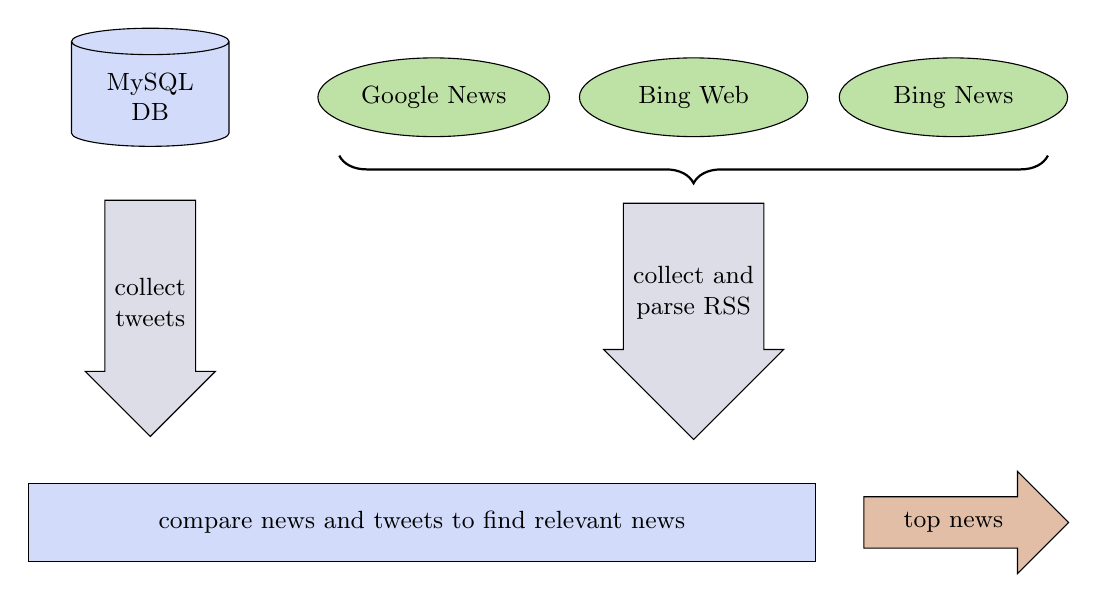
\begin{tikzpicture}[scale=.6,database/.style={
      cylinder,
      cylinder uses custom fill,
      cylinder body fill=lblue,
      cylinder end fill=lblue,
      shape border rotate=90,
      aspect=0.25,
      align=center,
      draw
    }]
\definecolor{silver}{RGB}{158,158,169}
\definecolor{midgray}{rgb}{.35,.35,.35}
\definecolor{lightsilver}{RGB}{221,221,232}
\definecolor{lblue}{RGB}{210,220,250}
\definecolor{mblue}{RGB}{165,190,225}
\definecolor{dblue}{RGB}{0,70,117}
\definecolor{lgreen}{RGB}{200,245,185}
\definecolor{mgreen}{RGB}{190,225,165}
\definecolor{mred}{RGB}{225,190,165}
\definecolor{dgreen}{RGB}{40,135,40}
\definecolor{dred}{RGB}{135,40,40}
    
\node[ellipse,fill=mgreen,draw=black,align=center,font=\small, minimum height=1cm, minimum width= 2.9cm] (ne1) at (6, 0) {Google News};3
\node[ellipse,fill=mgreen,draw=black,align=center,font=\small, minimum height=1cm, minimum width= 2.9cm] (ne2) at (11.5, 0) {Bing Web};
\node[ellipse,fill=mgreen,draw=black,align=center,font=\small, minimum height=1cm, minimum width= 2.9cm] (ne3) at (17, 0) {Bing News};

\visible<2->{
\draw [decorate,thick,decoration={brace,amplitude=10pt,mirror,raise=4pt}]
(4,-1) -- (19,-1);
\node[single arrow, draw, fill=lightsilver, align=center, shape border rotate=270, minimum height=3cm,font=\small](parse) at (11.5, -4) {\ \\ collect and\\ parse RSS};
}

\visible<3->{
\node[database, minimum width=2cm, minimum height=1.5cm, font=\small] (db) at (0,0) {MySQL \\ DB};
\node[single arrow, draw, fill=lightsilver, align=center, shape border rotate=270, minimum height=3cm,font=\small](parse) at (0, -4.2) {\ \\ collect\\ tweets};
}

\visible<4->{
\node[fill=lblue,draw=black,align=center,font=\small, minimum height=1cm, minimum width= 10cm] (ne3) at (5.75, -9) {compare news and tweets to find relevant news};
\node[single arrow, draw, fill=mred, align=center, shape border rotate=0,font=\small, minimum height=2.6cm, minimum width=1.3cm](parse) at (17,-9) {top news};
}

\end{tikzpicture}
}
\end{center}
%\section{Frontend}
\section{Frontend}
\label{sec:frontend}
\subsection{Design}

\subsubsection{Grober Entwurf}
Zu Beginn der Entwicklung des Frontend stand die Frage nach dem Aussehen und dem grundsätzlichen Aufbau im Raum. Es bestand der Wunsch nach einem übersichtlichen und vor allem intuitiv bedienbarem Interface. Erste Überlegungen und Skizzen führten schnell zu der Idee, das Grundlayout an bekannte und erfolgreiche Portale wie Google oder Wolfram Alpha anzulehnen. Die Startseite von TMetrics besteht also lediglich aus einem zentralen Eingabefeld mit darüber angeordnetem Logo und einigen weiteren Einstellungs- und Informationsmöglichkeiten als eine Leiste am oberen Rand.

\subsubsection{Erstes Konzept: Tabelle}
\label{sec:konzeptTabelle}

\begin{figure}[h!]
 \centering
 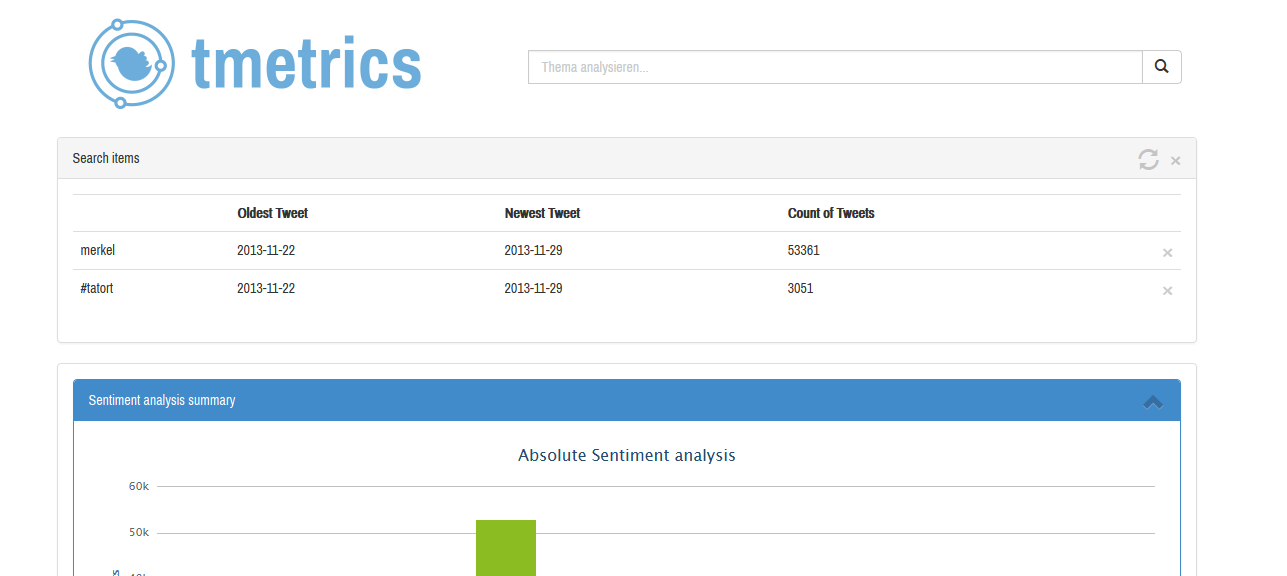
\includegraphics[width=0.8\textwidth]{./Bilder/Frontend/Screenshots/tabelleninterface.png}
\caption{Tabellarische Darstellung der Suchbegriffe}
\label{img:tabelle}
\end{figure}

Für die weiteren Ansichten wurde ein Konzept erarbeitet, welches diese Einfachheit und Übersichtlichkeit fortführen sollte. Grundsätzlich wurden das Logo und die Suchleiste verkleinert, weiter nach oben gerückt und nebeneinander anstatt untereinander angeordnet. Als dann die ersten Ergebnisse wie die Anzahl der gefundenen Tweets zu einem Suchbegriff, Datum der ersten und der neusten Suche zur Verfügung standen, wurden diese Daten tabellarisch dargestellt. Darunter wurden nach und nach untereinander die einzelnen Auswertungen hinzugefügt (siehe Abbildung \ref{img:tabelle}).

Nach der Eingabe eines weiteren neuen Begriffes öffnete sich zunächst immer die Vergleichsansicht. Dies entsprach grundsätzlich der Intention des gesamten Projektes, einzelne Begriffe miteinander vergleichen zu können. Um eine ausführlichere Auswertung zu einem einzelnen Begriff angezeigt zu bekommen, genügte ein Klick auf die jeweilige Tabellenzeile.

Im weiteren Verlauf des Projektes stellte sich doch heraus, dass dieses Bedienkonzept nicht besonders intuitiv zu sein schien. So musste für einen Wechsel zwischen der detaillierten Einzelansicht zweier verschiedener Begriffe mehrfach geklickt werden, was teilweise für den Benutzer nicht direkt nachvollziehbar war.

Außerdem stellte sich heraus, dass mit steigender Anzahl von Analyseansichten der Platz durch die Tabelle direkt im zentralen Fokus des Benutzers eher verschwendet wurde, anstatt diese Fläche mit einer höheren Informationsdichte z.B. in Form einer Analyse zu füllen. Nicht nur der Kunde, sondern auch die Entwickler merkten schnell, dass man hier viel scrollen musste, um die einzelnen Auswertungen dargestellt zu bekommen.

\subsubsection{Zweites Konzept: Kacheln}
\label{sec:konzeptKacheln}

\begin{figure}[h!]
 \centering
 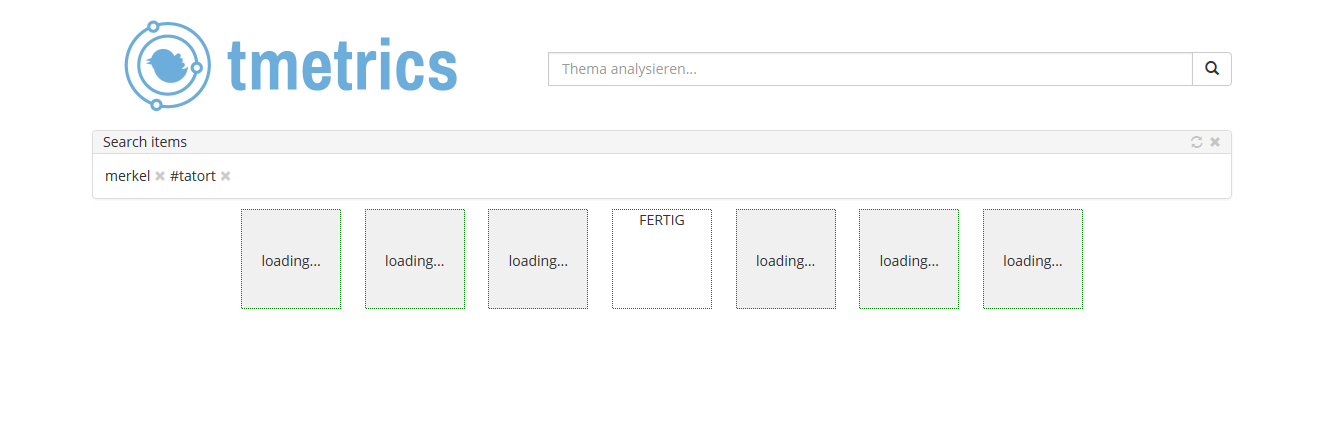
\includegraphics[width=0.8\textwidth]{./Bilder/Frontend/Screenshots/kachelinterface.png}
\caption{Erster Entwurf des Interfaces mit Kacheln, Arbeitsversion}
\label{img:kachel}
\end{figure}

In einem Sprint-Review schlug der Kunde also ein "`Kachelinterface"' vor. Der Hintergedanke des Kunden dabei war, dass ein "`exploratives"' Arbeiten ermöglicht werden sollte, indem man alle Auswertungen als mehr oder weniger große Kacheln direkt zu sehen bekommt und man durch ein Anklicken dieser Kachel in diese Analyseansicht "`hineingeht"', man sozusagen auch optisch und informativ in die Tiefe geht und dort dann die Details der jeweiligen Analyse angezeigt bekommt.

Während im Entwicklerteam die ersten Ideen und Ansätze (siehe Abbildung \ref{img:kachel}) zur Umsetzung heranreiften, stellte sich heraus, dass dies an vielen Stellen im Frontend einer völligen Neuentwicklung gleich käme, sich also nur mit erheblichem Aufwand umsetzen ließe. Außerdem fiel anhand erster Skizzen und Überlegungen zur optischen Gestaltung schnell auf, dass man hier für den eigentlich als essentiell erachteten Vergleich einer bestimmten Analyse zweier verschiedener Begriffe nur noch umständlich zugreifen kann. Grob umschrieben hätte sich der Interaktionsablauf so dargestellt, dass man eine geöffnete Analyse erst hätte schließen müssen, dann den Begriff wechseln um erneut im explorativen Stil wieder in die Tiefe gehen zu müssen.

Aus diesen Gründen beschäftigte sich das Team mit einem alternativen Ansatz. 

\subsubsection{Finales Konzept: Tabs}
\label{sec:konzeptTabs}
Erste Ideen zu diesem Konzept ergaben sich bereits während der Betrachtungen des Kachelinterfaces. Nachdem das Team diese Überlegungen weiter ausführte und gemeinsam mögliche Schwachstellen beseitigte wurde das neue Konzept dem Kunden in einem gesondertem Termin vorgestellt. Dieser war von der Idee begeistert und gab grünes Licht für die Umsetzung.
Das Konzept lehnt sich an das Kachelinterface des Kunden an, verbindet aber auch weitere bekannte strukturgebende Elemente wie z.B. verschiedene Tabs. Die Kacheln wurden aufgegriffen, um die Auswahl der zur Verfügung stehenden Analysemöglichkeiten darzustellen. Hier kann der Kunde die gerade aktiven und für alle Suchbegriffe gültigen Analysen einzeln aktivieren oder wieder deaktivieren. Diese Kachelansicht enthält exemplarische Darstellungen und kurze Beschreibungen der jeweiligen Analysen. Für einzelne Suchbegriffe werden nun Reiter anstelle von Tabelleneinträgen genutzt, diese können wie man es von modernen Browsern gewöhnt ist natürlich auch wieder geschlossen werden. Sobald mehr als ein Suchbegriff als Reiter geöffnet ist, erscheint als zusätzlicher Reiter ganz rechts der Comparison-Tab. Hier ist die Darstellung des direkten Vergleichs zweier Begriffe wiederzufinden. Aber auch der Vergleich anderer Analysen zu unterschiedlichen Begriffen ist mit diesem Konzept für den Benutzer deutlich einfacher zu realisieren. So kann er in der Analyseauswahl einfach nur die Analysen aktivieren, die für ihn gerade von Interesse sind. Um zwischen den Analysen der jeweiligen Begriffe hin- und herzuschalten, genügt jetzt ein einziger Klick auf den jeweiligen Tab.

Das ursprüngliche Ziel, ein simples und vor allem intuitives Interface zu gestalten, wurde durch die Verwendung von Reitern und weiteren bekannten optischen Elementen wie z.B. einem geöffnetem bzw. geschlossenem Auge zur Darstellung der aktiven bzw. inaktiven Analysen wieder erreicht.

\subsection{Verwendete Technologien}
Bereits vor und während der Phase eines ersten Entwurfs überlegten wir uns, welche externen Technologien und Bibliotheken uns bei der Entwicklung eines Frontends im Browser möglichst gut unterstützen könnten.

Dabei fiel schnell die Entscheidung, das HTML5-Framework Bootstrap \cite{Bootstrap} einzusetzen. Zwar muss man sich zusätzlich in dieses Framework einarbeiten und HTML5-Frameworks sind generell nicht mit älteren Browsern (wie beispielsweise Internet Explorer 8 oder älter) kompatibel, aber dafür bieten HTML5-Frameworks und im Speziellen Bootstrap auch zahlreiche Vorteile: Mit Hilfe vordefinierter Elemente (Icons, Buttons, Tabs, modale Dialoge, u.v.m.) sowohl in CSS als auch teilweise in JavaScript ist es möglich, ein homogenes Gesamtbild der Oberfläche zu erreichen, ohne selbst viele Anpassungen diesbezüglich machen zu müssen. Außerdem ist Bootstrap zu vielen aktuellen Browsern kompatibel, ohne dass der Entwickler einen Mehraufwand bzgl. der Kompatibilität betreiben muss \cite{BootstrapCompatibility}. Dies verdeutlicht Tabelle \ref{fig:BootstrapTab} anhand der Darstellung eines Buttons in verschiedenen Browsern mit und ohne Bootstrap.

Ebenfalls integriert ist der Ansatz von \textit{responsive webdesign}, das heißt, dass sich der Aufbau der Seite an das Endgerät des Benutzers anpassen kann, wofür im Allgemeinen CSS Media Queries \cite{CSSMediaQueries} eingesetzt werden. Beispielsweise ist es mit CSS Media Queries möglich, die Darstellung von HTML-Elementen an die Breite des Ausgabegerätes anzupassen. Speziell für Bootstrap spricht, dass der Quellcode frei verfügbar ist, viele Menschen es nutzen und somit auch viele Möglichkeiten für Hilfestellungen existieren, sowie die zahlreichen, verfügbaren Beispiele auf der Homepage, die gut dokumentiert sind.

\begin{table}[ht]
\centering
\small
\begin{tabular}{>{\raggedleft}c | m{2.25cm} | m{2.25cm} | m{2.25cm} | m{2.25cm}}
\toprule
 & Firefox & Chrome\newline(Windows) & IE 10 & Chrome\newline(Android)\\
\midrule
mit Bootstrap &

\includegraphics[width=2cm]{./Bilder/Frontend/Buttons/firefoxWith.png} &

\includegraphics[width=2cm]{./Bilder/Frontend/Buttons/chromeWith.png} &

\includegraphics[width=2cm]{./Bilder/Frontend/Buttons/ieWith.png} &

\includegraphics[width=2cm]{./Bilder/Frontend/Buttons/androidWith.png}
\\
\midrule
ohne Bootstrap &

\includegraphics[width=2cm]{./Bilder/Frontend/Buttons/firefoxWithout.png} &

\includegraphics[width=2cm]{./Bilder/Frontend/Buttons/chromeWithout.png} &

\includegraphics[width=2cm]{./Bilder/Frontend/Buttons/ieWithout.png} &

\includegraphics[width=2cm]{./Bilder/Frontend/Buttons/androidWithout.png}
\\
\bottomrule
\end{tabular} 
\caption{Vergleich der Darstellung eines Buttons in verschiedenen Browsern mit und ohne Bootstrap}
\label{fig:BootstrapTab}
\end{table}

Mit der Entscheidung für Bootstrap ging auch die Entscheidung für jQuery \cite{jQuery} als Werkzeug zur Navigation und Manipulation des Document Object Models, einem Interface zum dynamischen Zugriff auf die Struktur, den Inhalt und den Stil eines Dokuments, einher. Dies ist dadurch begründet, dass einerseits alle JavaScript-Elemente von Bootstrap jQuery benötigen und wir andererseits aus Erfahrung wussten, dass eine Bibliothek wie jQuery die Gestaltung einer Oberfläche mit Hilfe von JavaScript erheblich vereinfacht.

Zusätzlich zu diesen beiden Bibliotheken, die einen Rahmen zur Entwicklung der Oberfläche bieten, verwenden wir auch für die Darstellung der einzelnen Auswertungen zwei externe Bibliotheken.
Dies ist erstens Highcharts \cite{Highcharts}, welches die Darstellung verschiedener Graphen (beispielsweise Punktwolken, Balken- oder Kuchendiagramme) übernimmt. In der finalen Version unseres Systems wird Highcharts für die Darstellung von sieben der acht verfügbaren Auswertungen verwendet.
Für die Darstellung der achten Auswertung (namentlich die Ansicht \texttt{tagCloud}) verwenden wir die D3 Word Cloud \cite{D3TagCloud}, welche Anordnung, Sklaierung und Färbung der Wörter in der Tag Cloud berechnet und anschließend darstellt.

\subsection{Datenhaltung}
Bereits während der ersten Iteration unseres Projekts ergab sich das Bedürfnis, Antworten des REST-Services zwischenzuspeichern, solange sich der Benutzer auf TMetrics befindet, um möglichst selten neue Anfragen an den REST-Service senden zu müssen. Dies wurde vor allem dann deutlich, wenn bereits mindestens zwei Suchbegriffe eingegeben waren und man zwischen diesen hin- und herwechselte. Bei jedem Wechsel wurden die Anfragen für alle Auswertungen zum Suchbegriff, auf den man wechselte, neu abgeschickt.
Die erste Idee, diesem Problem zu entgegnen, war eine Zwischenspeicherung der Daten im Frontend. Da es sich bei den Antworten des REST-Services wie in Abschnitt \ref{sec:architekturDarstellung}
erwähnt um JSON-Objekte handelt, war eine Speicherung dieser ohne großen Zusatzaufwand möglich. Die Frage war nun, wo diese JSON-Objekte abgespeichert werden sollten. Da jedes JSON-Objekt immer genau einem Suchbegriff und einem Suchbegriff mehrere JSON-Objekte (für jede Auswertung ein Objekt) zugeordnet waren, war die erste Idee die in \texttt{jQuery} enthaltene Funktion \texttt{data(key, value)} zu nutzen. Diese Funktion speichert zu einem oder mehreren HTML-Elementen ein beliebiges JavaScript-Objekt \texttt{value} unter dem Schlüssel \texttt{key} ab. Das abgespeicherte Objekt kann mit der Funktion \texttt{data(key)} und demselben Schlüssel dann wieder abgerufen werden \cite{jQueryData}.

Da in der ersten Version des Frontends zu jedem Suchbegriff auch eine Zeile in der in Abschnitt \ref{sec:konzeptTabelle} beschriebenen Tabelle, also ein \texttt{<tr>}-Element, existierte, war die Idee jeder Anfrage einen eindeutigen Schlüsselnamen zu geben und so das entsprechende JSON-Objekt mit diesem Schlüsselnamen an der zu diesem Suchbegriff passenden Tabellenzeile zu speichern. Beim Abrufen einer Auswertung wurde dann, falls verfügbar, auf das zwischengespeicherte JSON-Objekt zugegriffen und ansonsten eine neue Anfrage an den REST-Service gestellt.

Allerdings war diese Umsetzung der Datenhaltung an die Darstellung als Tabelle gebunden, was bei der Umstellung auf ein neues Darstellungskonzept, wie in \ref{sec:konzeptKacheln} beschrieben, zu Problemen führte. Es wäre möglich gewesen, die Daten nun an den neuen HTML-Objekten zu speichern, was das Problem allerdings nur temporär bis zur eventuell nächsten Umstellung des Designs gelöst hätte.
Für eine langfristige Lösung war es also von Nöten, Datenhaltung und Darstellung unabhängig voneinander zu gestalten.

\begin{figure}
 \centering
 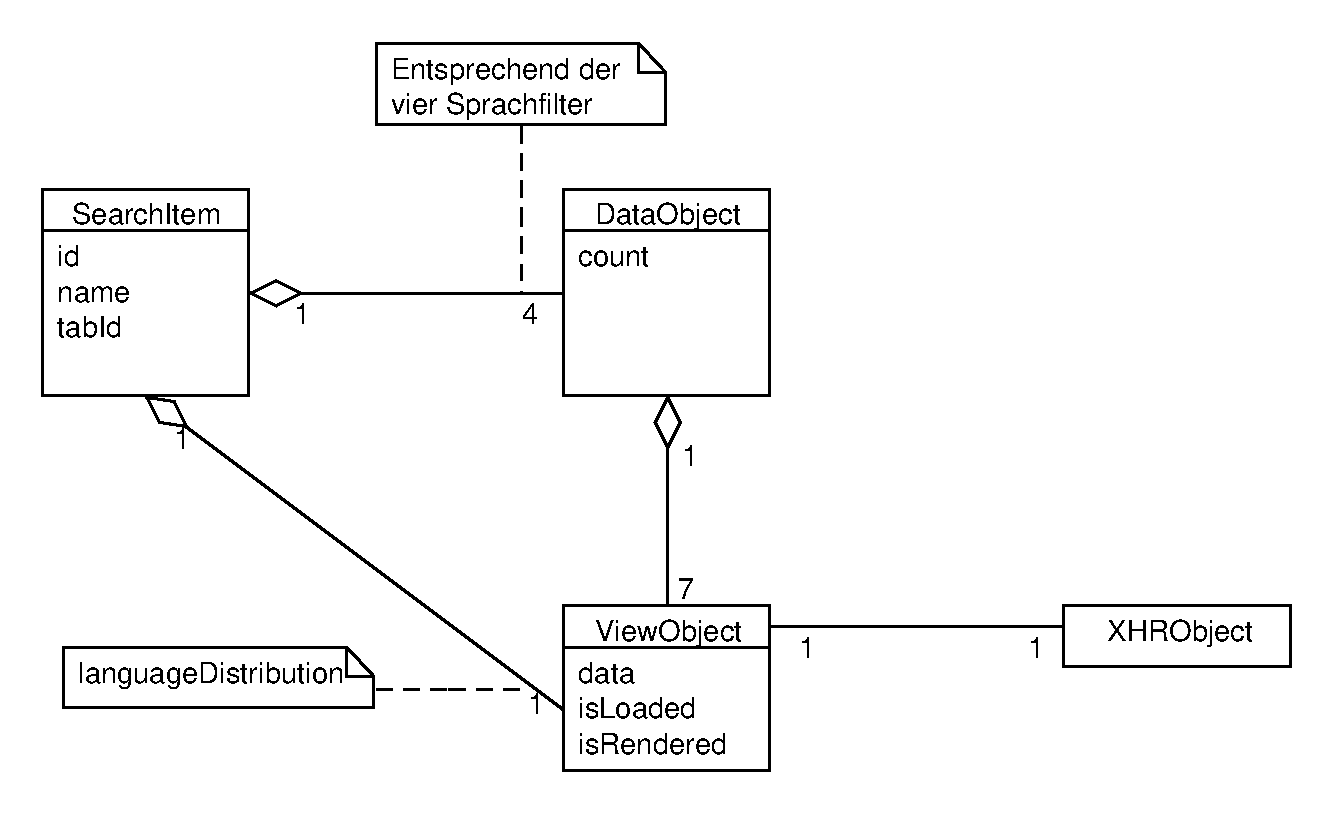
\includegraphics[width=0.8\textwidth]{./Bilder/Frontend/classDiagram.pdf}
\caption{Klassendiagramm der Datenhaltung im Frontend}
\label{img:FrontEndClassDiagram}
\end{figure} 

Die Umsetzung dieser Idee ist in der in Abbildung
\ref{img:FrontEndClassDiagram}
dargestellten Klassenstruktur eines globalen Arrays von Suchbegriffen gemündet. Dabei wird für jeden Suchbegriff (Klasse \texttt{SearchItem}) zwischen vier vordefinierten Sprachfiltern (keine Filterung, englisch, deutsch und eine beliebige weitere Sprache; Klasse \texttt{DataObject}) und in jedem Filter nochmals zwischen den acht verfügbaren Ansichten (Klasse \texttt{ViewObject}) unterschieden. Die einzige Ausnahme hiervon bildet die Ansicht \texttt{languageDistribution}, weil diese unabhängig vom eingestellten Sprachfilter ist und daher nur einmal pro Suchbegriff gespeichert werden muss.
Als zusätzliche Information wird zu jedem \texttt{DataObject} abgespeichert, wie viele Tweets zu diesem Suchbegriff mit dem jeweiligen Sprachfilter vorliegen.
Zu jeder einzelnen Ansicht wird wiederum einerseits, falls vorhanden, das JSON-Objekt der Antwort einer Anfrage des REST-Services zusammen mit den Informationen, ob die Ansicht fertig geladen und gerendert wurde (jeweils als \texttt{boolean}-Flag), gespeichert. Andererseits wird die REST-Anfrage selbst als eigenes Objekt \texttt{XHRObject} für die Verwendung in den \textit{connection pools} gespeichert, die im nächsten Abschnitt \ref{sec:conPool} beschrieben werden.
Außerdem sind noch der aktive Tab, der aktive Sprachfilter und ein \texttt{boolean}-Array, das angibt, welche Ansichten sichtbar bzw. nicht sichtbar sind, global verfügbar, sodass jederzeit bekannt ist, welche Ansichten der Benutzer aktuell angezeigt bekommt und welche Daten dafür benötigt werden.

Zusätzlich zu der gerade beschriebenen flüchtigen Speicherung von Daten im Frontend, wird auch eine persistente Speicherung für benutzerspezifische Einstellungen verwendet. Dabei werden die Einstellungen zur Sichtbarkeit der Ansichten und der gewählte Sprachfilter über den \texttt{localStorage} \cite{WebStorage} client-seitig gespeichert. Zudem werden auch die aktuellen Suchbegriffe gespeichert, sodass diese beim nächsten Besuch von TMetrics dem Benutzer in einem Dropdown-Menü zur erneuten Analyse vorgeschlagen werden. Hierbei werden aber immer nur die Suchbegriffe des direkten vorherigen Besuchs gespeichert.

\subsection{Connection Pools}
\label{sec:conPool}
\subsubsection{Problematik}
Bedingt durch die REST-Architektur unseres Systems und die Entscheidung, einzelne Ansichten unabh"angig voneinander aufrufen zu k"onnen, wird in unserem System f"ur jede Ansicht (einen Überblick über die Ansichten von TMetrics wurden in Abschnitt \ref{sec:umgesetztesSystem} gegeben und sind in Abbildung \ref{fig:viewScreenshots} zu sehen) eine Anfrage an den REST-Service gestellt. 
Alle g"angigen Browser unterst"utzen aber nur eine gewisse Anzahl an parallelen Verbindungen pro Server (siehe Tabelle \ref{fig:ConPoolTab}). Das Minimum der Anzahl paralleler Verbindungen zu einem Server unter den von uns unterst"utzen Browsern liegt bei sechs. 

\begin{table}[ht]
\centering
\small
\begin{tabular}{l | c c c c c c c}
\toprule
Browser & Parallele Verbindungen\\
\midrule
Chrome 4+ & 6\\
Firefox 3+ & 6\\
IE 8 \& 9 & 6\\
IE 10 & 8\\
Opera 10 & 8\\
Opera 11+ & 6\\
Safari 4+ & 6\\ 
\bottomrule
\end{tabular} 
\caption{Anzahl paralleler Verbindungen zu einem Server verschiedener Browser und Versionen \cite{BrowserScope}.}
\label{fig:ConPoolTab}
\end{table}

Gibt der Benutzer im Frontend einen Suchbegriff ein und schickt diesen ab, so werden f"ur die Ansichten bereits acht Anfragen an den REST-Service geschickt, was  acht parallelen Verbindungen zu einem Server entspricht. Der Browser des Benutzers wird in diesem Fall aber zun"achst nur so viele Anfragen abschicken, wie seine Konfiguration es zulässt. Wie oben beschrieben gehen wir hierbei im schlechtesten Fall von sechs Anfragen aus. Die verbleibenden anderen beiden Anfragen werden solange zur"uckgehalten, bis auf eine der vorherigen eine Antwort des REST-Services kommt.

Dies ist soweit noch kein Problem, da der Benutzer lediglich f"ur zwei Auswertungen l"anger warten muss, als diese Auswertungen eigentlich an Zeit ben"otigen. Problematisch wird es, wenn der Benutzer direkt nach Eingeben des ersten Suchbegriffs einen weiteren Suchbegriff eingibt, da auch dabei schon bevor die acht Anfragen der Auswertungen abgeschickt werden, bis zu zwei weitere sequentielle Anfragen an den REST-Service geschickt werden. Zuerst die Anfrage, ob der Suchbegriff bereits in der Datenbank vorliegt und falls dies zutrifft die Anfrage, die die interne ID dieses Suchbegriffs zur"uckliefert. Erst nach der Antwort auf diese beiden initialen Anfragen wird dem Benutzer ein Feedback im Frontend in Form des Erscheinen eines neuen Tabs für den soeben abgeschickten Suchbegriff gegeben und die Anfragen der einzelnen Ansichten werden abgeschickt.

Im ung"unstigen Fall, dass nun alle sechs Verbindungen zum Server durch Anfragen der Ansichten belegt sind, wird beim Abschicken eines neuen Suchbegriffs die Anfrage, ob dieser Begriff bereits in der Datenbank vorliegt, zun"achst nicht abgeschickt und der Benutzer bekommt somit auch kein Feedback vom Frontend.

Zur L"osung dieser Problematik haben wir zwei Ans"atze in Betracht gezogen. Erstens das Zusammenf"uhren von Anfragen, sodass wir insgesamt deutlich weniger Verbindungen pro Server ben"otigen und zweitens die Einf"uhrung eines Verwaltungssystems f"ur Anfragen, sodass wir an Stelle des Browsers regeln, welche Anfragen gestartet und welche noch warten sollen.
Das f"ur unsere Entscheidung ausschlaggebende Argument war, dass f"ur den Benutzer h"aufig nicht alle Ansichten relevant sind. Das hei\ss{}t, dass er in den Einstellungen zur Sichtbarkeit die Ansichten ausgew"ahlt hat, die er angezeigt bekommen m"ochte. Unser System sollte also die Anfragen zu diesen Ansichten bevorzugt behandeln. Dies w"are mit dem ersten L"osungsvorschlag nicht m"oglich, da alle Anfragen zu einer geb"undelt w"urden und eine Antwort auf diese geb"undelte Anfrage erst k"ame, wenn alle Teilauswertungen vom REST-Service bearbeitet w"aren.
Der Benutzer m"usste also im schlimmsten Fall auf die Auswertung einer Ansicht warten, die er nicht sehen m"ochte.
Unser L"osungsansatz ist also die Einf"uhrung eines Verwaltungssystems f"ur Anfragen, welches wir \textit{connection pools} nennen.

\subsubsection{Aufbau}
Die Idee der \textit{connection pools} ist es, Anfragen nach Priorit"aten zu behandeln und abzuarbeiten. Dabei gibt es folgende drei Priorit"aten: passiv, aktiv und spezial. F"ur jede existiert jeweils ein Pool mit momentan in Bearbeitung stehenden Anfragen und eine Warteschlange f"ur noch zu bearbeitende Anfragen. Die Aufgabe der \textit{connection pools} ist es nun, daf"ur zu sorgen, dass einerseits in den Pools der drei Priorit"aten zusammen maximal sechs Verbindungen zum Server existieren und andererseits die Pools mit Anfragen aus den Warteschlangen aufgef"ullt werden, wenn eine Anfrage abgearbeitet wurde.

\subsubsection{Umsetzung}
Zur Realisierung dieser Aufgaben wird jedem der drei Pools eine feste Anzahl an erlaubten Verbindungen zum Server, sogenannte Slots, zugeteilt. In unserem System stehen f"ur den Spezial-Pool ein, f"ur den Aktiv-Pool drei und f"ur den Passiv-Pool zwei Slots zur Verf"ugung. Diese Zuteilung ergab sich aus der Überlegung, welche Anfrage mit einer bestimmten Priorit"at in welcher H"aufigkeit auftritt.

Da nur die Anfragen nach der ID eines Suchbegriffs und ob ein Suchbegriff bereits in der Datenbank vorliegt, die Priorit"at spezial haben und diese Anfragen nie parallel ausgef"uhrt werden, gen"ugt logischerweise ein Slot f"ur den Spezial-Pool. Diese Anfragen sollten also schnellstmöglich abgeschickt werden, um das eingangs genannte Problem zu lösen. Alle anderen Anfragen haben entweder die Priorit"at aktiv, wenn der Benutzer die Ergebnisse der Anfrage direkt angezeigt bekommen soll oder passiv, falls die Anfrage nur im Hintergrund l"auft und Ergebnisse dann auf Abruf bereit stehen sollen. Dies ist abh"angig vom aktiven Tab, dem ausgew"ahlten Sprachfilter, sowie der Einstellung f"ur die Sichtbarkeit der einzelnen Ansichten.
Eine andere Verteilung der Slots von Passiv- und Aktiv-Pool ist auch m"oglich und einfach im Code anzupassen.

Bei den Warteschlangen handelt es sich um Stacks bzw. LIFO-Warteschlangen. Dies hat den Hintergrund dass wir dem Benutzer generell das Ergebnis, auf die von ihm zuletzt ausgef"uhrte Aktion am schnellsten liefern möchten, damit die aktuelle Anzeige im Frontend mit Daten gefüllt ist.

Ein weitere Idee der Umsetzung der \textit{connection pools} ist es, dass auf Eingaben des Benutzers angemessen reagiert wird. Das bedeutet, dass die Priorit"aten von Anfragen ge"andert werden, wenn sich die Sichtbarkeit der zugeh"origen Ansichten als Folge einer Nutzereingabe "andert. Dies kann durch Wechsel des Tabs, des Sprachfilters oder der Sichtbarkeitseinstellung geschehen. Eine Anfrage zu einer Ansicht, die nicht mehr sichtbar ist, wird, sofern sie noch nicht fertig abgearbeitet ist, abgebrochen und in den Passiv-Pool bzw. in die Passiv-Warteschlange verschoben. Im umgekehrten Fall wird in den Aktiv-Pool bzw. in die Aktiv-Warteschlange verschoben.
So wird sichergestellt, dass die Priorit"aten aller Anfragen zu jeder Zeit an die Aktionen des Nutzers angepasst sind und Anfragen relevanter Ansichten m"oglichst schnell bearbeitet werden.

\subsubsection{Fazit}
Ein Problem der \textit{connection pools} ist es, dass damit nur Anfragen verwaltet werden, die wir auch aktiv zuweisen. Dies ist bei Anfragen, die "uber externe Bibliotheken abgeschickt werden, nicht ohne Weiteres m"oglich. Dies betrifft in unserem System die Autovervollst"andigung bei Eingabe eines Suchbegriffs. In diesem Fall wird in der Bibliothek \texttt{typeahead.js} \cite{typeahead}
geregelt, wann genau eine Anfrage abgeschickt wird und wir k"onnen sie daher nicht in die \textit{connection pools} einpflegen. Um dieses Problem zu l"osen, w"are eine Anpassung der externen Bibliothek n"otig.

Ein weiteres mit den \textit{connection pools} verbundenes Problem ist die teilweise schlechte Auslastung der einzelnen Pools. Da eine Anfrage eine festgelegte Priorit"at hat, ist sie auch fest einem Pool, bzw. einer Warteschlange zugeordnet. Will der Benutzer aber beispielsweise die Auswertungen zu allen Ansichten haben, so werden acht Anfragen an die Connection Pools gesendet, von denen aber nur drei direkt abgeschickt werden, da der Aktiv-Pool nur drei Slots hat. Ohne die \textit{connection pools} w"aren an dieser Stelle sechs Anfragen abgeschickt worden. Eine m"ogliche L"osung w"are die Nutzung von Pools anderer Priorit"aten unter der Bedingung, dass diese entweder frei sind oder eine niedrigere Priorit"at haben. So w"urden Anfragen der Priorit"at aktiv nur den Spezial-Pool benutzen, wenn dieser frei w"are (und von m"oglicherweise ankommenden Anfragen mit Priorit"at spezial wieder verdr"angt werden). Der Passiv-Pool hingegen k"onnte direkt von Anfragen mit Priorit"at aktiv genutzt werden. Mögliche Anfragen der Priorität passiv sollten dabei von denen der Priorität aktiv verdrängt werden.

Zusammenfassend lässt sich sagen, dass die \textit{connection pools} eine funktionierende Umsetzung f"ur eine Verwaltung von Anfragen an den Server sind. Um die Effizienz voll auszureizen, sollten aber die in diesem Unterabschnitt genannten Probleme noch behoben werden.

\subsection{Besonderheiten}

In diesem Abschnitt werden weitere interessante Details der Implementierung oder Designentscheidungen, die wir bezüglich des Frontends getroffen haben, diskutiert.

\subsubsection{Anzahl an Tweets im zeitlichen Verlauf}

Die im Folgenden beschriebene Ansicht gibt an, wie viele Tweets zu einem gegebenen Suchbegriff in einem bestimmten Zeitraum veröffentlicht wurden.

Bei der ersten Implementierung dieser Ansicht haben wir festgelegt, dass die Tweets eines Tages jeweils addiert werden, sodass der Graph die Anzahl Tweets pro Tag widerspiegelte.
Wie in Abbildung \ref{fig:tphCompare} deutlich wird, wird die Auswertung vor allem bei Suchbegriffen, zu denen nur über einen verhältnismäßig kurzen Zeitraum Daten vorliegen, aussagekräftiger, wenn man den betrachteten Zeitraum von einem Tag auf eine Stunde verkürzt.

Aber auch hierbei ist eine weitere Optimierung denkbar, da die Anzahl Tweets pro Stunde an Aussagekraft verlieren, wenn man einen Datenbestand betrachtet, der sich über einen großen Zeitraum, beispielsweise mehrere Monate, erstreckt. Eine Anpassung des zusammenzufassenden Zeitraums in Abhängigkeit vom gesamten betrachteten Zeitraum wäre also wünschenswert, um diese Problematik zu lösen. Eine leichte Umsetzung dieser Idee ist allerdings nicht möglich, da Highcharts diese Funktionalität nicht nativ unterstützt und man dies manuell einbauen müsste.
Im Verlauf des Projektes wurde allerdings weitere Funktionalität in die hier beschriebene Ansicht eingefügt. Nachdem der Kundenwunsch nach explorativem Arbeiten in unserem System laut wurde, wurde einerseits das durch Klick auf den Graphen aufrufbare Anzeigen von einzelnen Tweets einer bestimmten Stunde (siehe Abschnitt \ref{sec:showTweets}) implementiert. Andererseits wurde dann auch noch das in Abschnitt \ref{sec:news} beschriebene News-Modul in diese Ansicht integriert. Details dazu sind den jeweiligen Abschnitten zu entnehmen.

\begin{figure}[ht]
\centering
\begin{subfigure}[t]{0.45\textwidth}
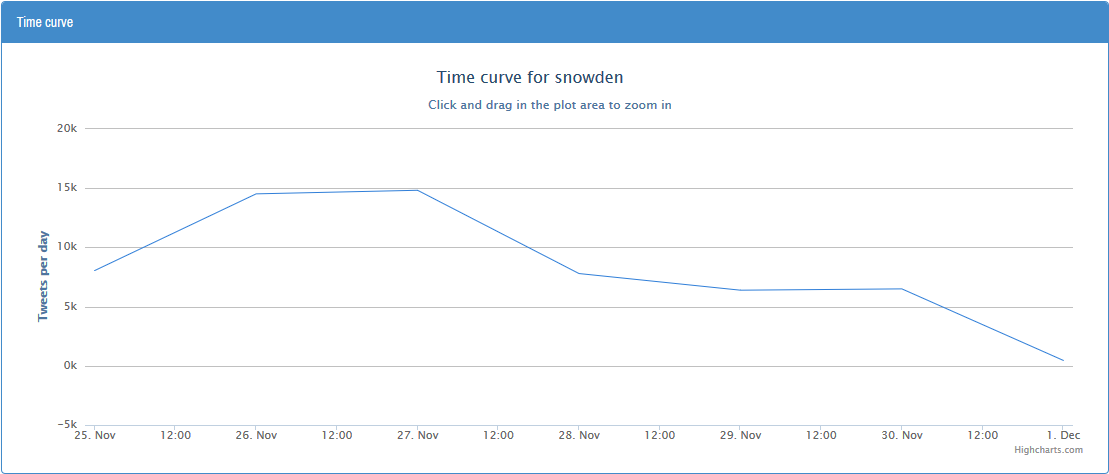
\includegraphics[width=\textwidth]{Bilder/Frontend/snowdenOld.png}
\caption{Tweets pro Tag}
\label{fig:tphDay}
\end{subfigure}
~
\begin{subfigure}[t]{0.45\textwidth}
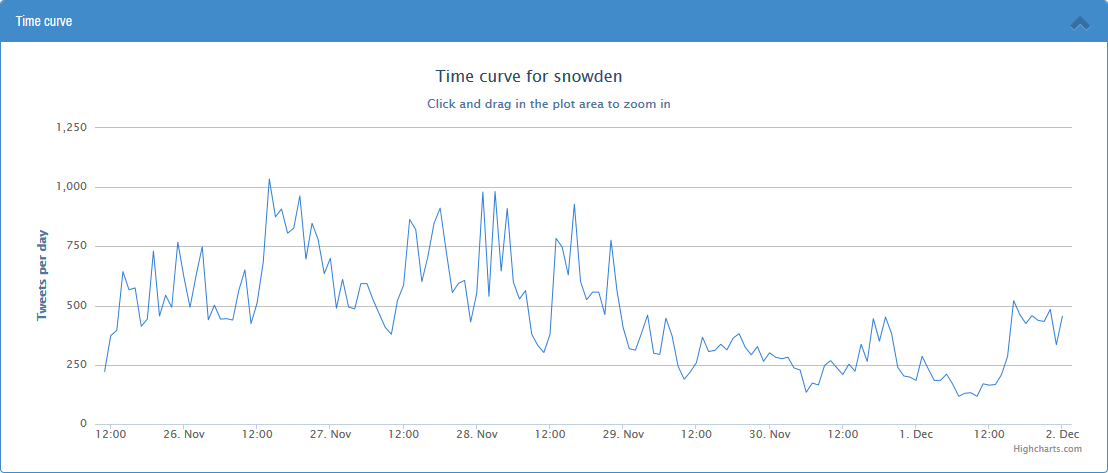
\includegraphics[width=\textwidth]{Bilder/Frontend/snowdenNew.png}
\caption{Tweets pro Stunde}
\label{fig:tphHour}
\end{subfigure}
\caption{Vergleich der Tweets im zeitlichen Verlauf pro Tag (links) und pro Stunde (rechts) zum Suchbegriff \glqq Snowden\grqq}
\label{fig:tphCompare}
\end{figure}

\subsubsection{Tweets anzeigen}
\label{sec:showTweets}
Wie bereits im vorigen Abschnitt erwähnt, bietet TMetrics die Möglichkeit, explorativ zu arbeiten und sich einzelne Tweets anzeigen zu lassen. Diese Funktionalität ist einerseits in der Auswertung der Sentiment-Analyse verfügbar und andererseits in der Ansicht der Anzahl Tweets im zeitlichen Verlauf. Aus der Sentiment-Analyse heraus werden je nachdem, welcher Teil des Balken- oder Kuchendiagramms angeklickt wurde, nur positive, nur negative oder nur neutrale Tweets angezeigt. Will man einzelne Tweets aus der Ansicht des zeitlichen Verlaufs heraus betrachten, so werden nur Tweets innerhalb des ausgewählten Zeitraums, also innerhalb einer bestimmten Stunde, angezeigt.

Unabhängig von der Ansicht, ist die Anzeige einzelner Tweets auf maximal 100 Tweets begrenzt. Eine solche Begrenzung ist sinnvoll, da sonst bei einem Suchbegriff mit großem Datenbestand sehr lange Ladezeiten verursacht werden können.
Um dem Nutzer nun dennoch möglichst repräsentative Tweets zeigen zu können, werden die Tweets nach Wichtigkeit sortiert. Als Maß für die Wichtigkeit eines Tweets sind verschiedene Möglichkeiten denkbar. Wir haben uns dafür entschieden, die Anzahl Retweets eines Tweets als alleiniges Maß für die Wichtigkeit eines Tweets zu nehmen. Grund für diese Entscheidung ist, dass die Anzahl Retweets ein eigenes Feld der Datenbank ist und wir daher effizient sortieren können, um die 100 wichtigsten Tweets zu finden. Da aber auch einem Retweet selbst dieselbe Anzahl an Retweets wie dem Original-Tweet zugeordnet ist, hat dies zur Folge, dass wir Retweets von der Anzeige ausschließen müssen, um eine mehrfache Anzeige des gleichen Tweets zu vermeiden. Es werden also die 100 Original-Tweets mit der höchsten Anzahl an Retweets angezeigt.

Ein weiteres Feature der Anzeige einzelner Tweets ist die Anzeige von weiteren Informationen zu diesem Tweet, die auf Wunsch abrufbar sind. So ist es durch einen einfachen Klick auf den Namen des Autors eines Tweets möglich, nähere Informationen über diesen einblenden zu lassen. Selbiges gilt auch für einen Klick auf den Text des Tweets, was eine Anzeige der Anzahl Retweets, der geografischen Koordinaten (falls verfügbar), der Sprache, sowie des Sentiments des Tweets zur Folge hat. Hier wird dem Benutzer wiederum die Möglichkeit gegeben, sich näher über die Einflussfaktoren des Sentiments zu informieren, was im folgenden Abschnitt \ref{sec:showTweetsSenti} näher erläutert wird. Bei der Designentscheidung war es besonders wichtig, den Fokus zunächst auf das Wesentliche -- also den Tweet selbst -- zu legen und trotzdem die Möglichkeit zu bieten, detaillierte Informationen dem Nutzer auf Abruf zur Verfügung zu stellen.

\subsubsection{Darstellung der Sentiment-Einflussfaktoren}
\label{sec:showTweetsSenti}
Aus dem Anspruch, dem Benutzer ein exploratives Arbeiten auf TMetrics zu ermöglichen, ergab sich im Projektverlauf die Anforderung, eine Möglichkeit zu liefern, die Einflussfaktoren bei der Bestimmung des Sentiments eines Tweets darzustellen. Grundsätzlich existieren dabei zwei Kategorien von Einflussfaktoren auf das Sentiment eines Tweets: ein vorbestimmtes Wörterbuch (für Wörter und Emoticons) mit festgelegten Sentiment-Werten sowie ein auf Trainingsdaten basierendes Regressionsmodell mit Werten für sämtliche Wörter (Unigrams) sowie Wortgruppen aus zwei bis vier Wörtern (Bigrams, Trigrams und Fourgrams, siehe auch Abschnitt \ref{sec:regressionmodel}).  Daraus ergeben sich insgesamt sechs Faktoren, deren Summe das Sentiment des Tweets bestimmt: Wörter, Emoticons, Unigrams, Bigrams, Trigrams und Fourgrams.

Da für jeden Faktor auch noch angegeben werden soll, wie die Wörter im Tweet den Einfluss dieses Faktors beeinflussen, muss eine Menge Informationen wiedergegeben werden. Zur gleichen Zeit sollte die Größe der Box zum Anzeigen eines Tweets möglichst gering sowie die Darstellung der und Navigation zwischen den Einflussfaktoren möglichst intuitiv gehalten werden. Die Umsetzung dieser Anforderungen ist im Anschluss beschrieben.

\begin{figure}[ht]
\centering
\begin{subfigure}[t]{0.45\textwidth}
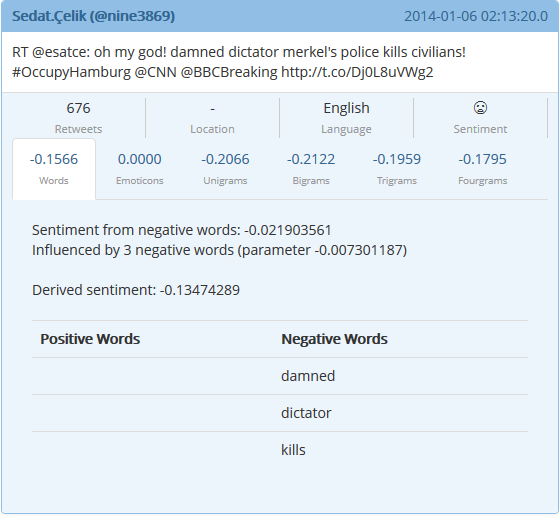
\includegraphics[width=\textwidth]{Bilder/Frontend/SentimentTweetsWords.png}
\caption{Wörterbuch}
\label{sentimenttweetswords}
\end{subfigure}
~
\begin{subfigure}[t]{0.45\textwidth}
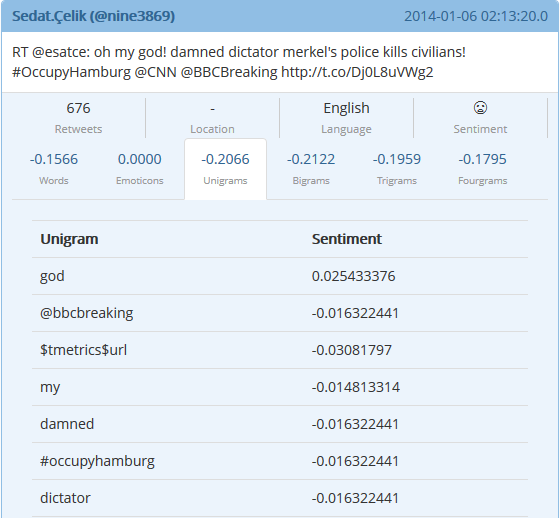
\includegraphics[width=\textwidth]{Bilder/Frontend/SentimentTweetsUnigrams.png}
\caption{n-Gramm}
\label{sentimenttweetsunigrams}
\end{subfigure}
\caption{Darstellung der Einflussfaktoren des Sentiments}
\label{sentimenttweets}
\end{figure}

Es wurde eine zusätzliche Ansicht hinzugefügt, die ausgehend von der Leiste mit den Metadaten durch Klick auf die Sentiment-Sparte ausgeklappt werden kann. Diese besteht dann aus sechs Tabs, welche den sechs genannten Einflussfaktoren entsprechen. Der Name des Reiters beinhaltet den Wert des Einflussfaktors, sodass die Summe der Werte aller Reiter dem Gesamtsentiment entspricht. Ein Klick auf den Reiter stellt eine detaillierte Auflistung dar, wie sein Wert aus dem Text des Tweets zustande kommt. Diese unterscheidet sich für die zwei eingangs genannten Kategorien.

Für Wörterbuch-Faktoren (in Abbildung \ref{sentimenttweetswords} exemplarisch für Wörter) basiert der Wert nur auf der Anzahl gefundener negativer bzw. positiver Wörter/Emoticons und einem zugehörigen Parameter. Ist mindestens ein solches Wort vorhanden, werden diese Werte und daraus berechnete (positive oder negative) Teil-Sentiment dargestellt. Der dabei dargestellte abgeleitete Sentiment-Wert ("`derived sentiment"') entspricht der Aggregationsfunktion zum Wörterbuch von Liu (siehe Abschnitt \ref{sec:sentimentclassifier}). Dieser wird immer angezeigt. Abschließend werden sämtliche im Wörterbuch vorkommenden Wörter des Tweets gelistet.

Die Darstellung der Details von Unigrams (für Unigrams in Abbildung \ref{sentimenttweetsunigrams} analog für Bigrams, Trigrams, Fourgrams) besteht nur aus einer tabellarischen Auflistung dieser n-Gramms des Tweets und der dazugehörigen Sentimentwerte (der Gesamtwert des Einflussfaktors entspricht der Summe seiner n-Gramms).

Zur besseren visuellen Aufbereitung dieser Informationen wird außerdem noch eine Einfärbung der n-Grams nach ihrem Sentiment-Wert vorgenommen. Dabei wurde die Konvention verwendet, neutrales Sentiment wie gewöhnlich in Schwarz darzustellen, während positives und negatives Sentiment in vier grünen bzw. roten Farbtönen mit zunehmender Sättigung dargestellt wird. Die dabei notwendige Festlegung wurde nach Betrachtung des Wertebereichs des Sentiments einzelner n-Grams intuitiv vorgenommen. Für positive n-Grams wurde festgestellt, dass nur sehr positive n-Grams den Wert 0.05 überschreiten, weshalb dies als untere Grenze für den grünen Farbton mit der höchsten Sättigung verwendet wurde. Weiterhin haben wir es als sinnvoll erachtet, dass nur dann ein positives Sentiment vorliegt, wenn die zweite Nachkommastelle nicht null ist. Daher wurde 0.1 als obere Grenze des neutralen Sentiments und damit als Untergrenze des grünen Farbtons mit der niedrigsten Sättigung verwendet. Danach fiel die Wahl auf 0.25 und 0.4 als Grenzwerte zwischen den übrigen Farbtönen. Da das Sentiment vom Modell her symmetrisch ist, wurden dieselben Grenzen im Negativen für die roten Farbtöne des negativen Sentiments verwendet. Da im Wörterbuch alle positiven Einträge gleich positiv und alle negativen Einträge gleich negativ sind, haben wir dort von einer Einfärbung abgesehen, da sie keine weiteren Informationen liefert.

Nachdem auf diese Weise bereits eine Heuristik zur Einfärbung von n-Grams implementiert worden ist, wurde die Entscheidung getroffen, sie auch auf den Gesamttext des Tweets anzuwenden. Eine Einfärbung auf Grundlage sämtlicher n-Grams ist dabei nicht praktikabel, da nicht für alle Wörter im Text ein eindeutiges Sentiment existiert. Es könnte z.B. ein Bigram mit negativem Sentiment existieren, das ein Unigram mit positivem Sentiment beinhaltet. Außerdem ist das Einfärben nur im Fall der Unigrams trivial, da sich dort der Text leicht in seine Wortbestandteile zerlegen lässt und sich diese anhand des Sentimentwertes des entsprechenden Unigrams einfärben lassen. Aus diesem Grund wurde das Einfärben nur für Unigrams umgesetzt. Die ursprüngliche Zielsetzung, die Einfärbung vom offenen Tab in der Ansicht der Einflussfaktoren abhängig zu machen und bei geschlossener Detailansicht gar keine Einfärbung im Volltext vorzunehmen, konnte aus Zeitgründen nicht umgesetzt werden, ist aber grundsätzlich möglich und sinnvoll. Unter diesen Umständen wäre es außerdem auch möglich, eine Einfärbung des Volltexts auf Grundlage des Wörterbuchs vorzunehmen. Beide Arten der Einfärbung sind in Abbildung \ref{sentimenttweetscolors} zu sehen.

\begin{figure}[ht]
\centering
\begin{subfigure}[t]{0.45\textwidth}
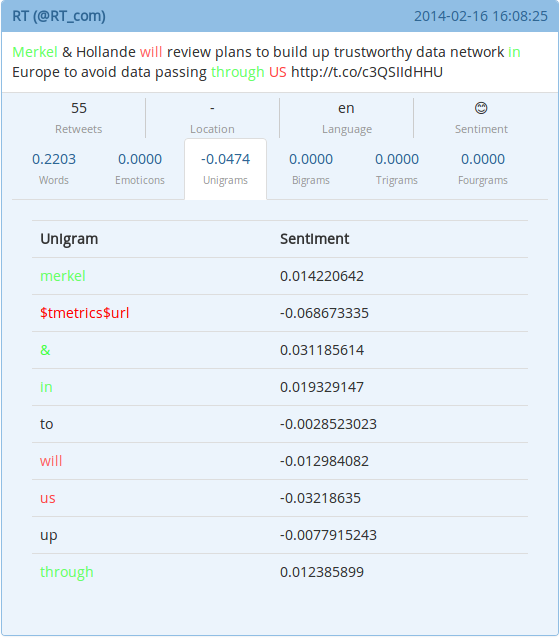
\includegraphics[width=\textwidth]{Bilder/Frontend/SentimentTweetsColors.png}
\caption{Einfärbung: n-Grams und Volltext}
\label{sentimenttweetscolors}
\end{subfigure}
~
\begin{subfigure}[t]{0.45\textwidth}
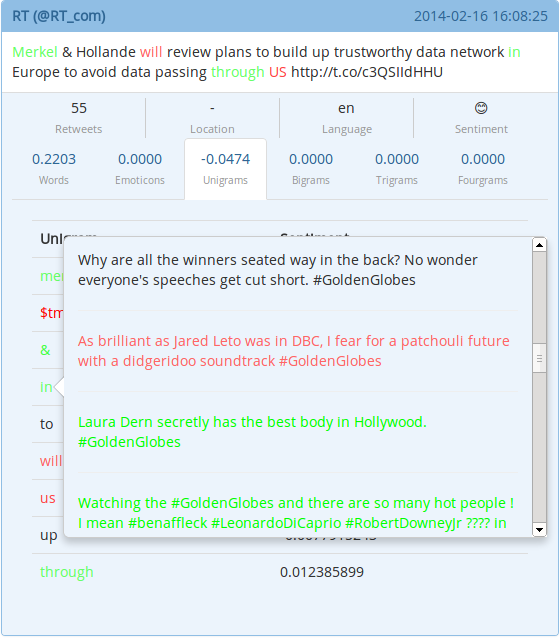
\includegraphics[width=\textwidth]{Bilder/Frontend/SentimentTrainingstweets.png}
\caption{Trainingstweets als Popover}
\label{trainingstweets}
\end{subfigure}
\caption{}
\end{figure}

Bei Betrachtung der Einflussfaktoren ist es möglich, dass die Fragestellung auftritt, wie das Sentiment dieses Faktors zustande gekommen ist (beispielsweise bei einem negativen Wert für ein intuitiv positives Wort). Aus diesem Grunde kann es von Interesse sein, sich die Trainingstweets anzuschauen, die zu dieser Bewertung des Sentiments geführt haben. Da unter Umständen viele Trainingstweets zu einem n-Gram vorliegen und jedes Mal deren Volltext dargestellt werden muss, stellt sich wieder die Herausforderung, diese Menge an zusätzlichen Informationen intuitiv und ohne Verkomplizierung des bestehenden Interfaces darzustellen. Dies wurde schlussendlich durch die Möglichkeit gewährleistet, auf ein n-Gram zu klicken und damit ein scrollbares Popover zu öffnen, welches nur den Text der relevanten Trainingstweets auflistet. Da Trainingstweets nur mit den Werten -1, -0.5, 0, 0.5 und 1 gelabelt werden können, ist es außerdem nicht notwendig, diese Werte explizit aufzulisten. Stattdessen wird das Labeling der Trainingstweets durch entsprechendes Einfärben des gesamten Textes in entsprechenden Farbtönen analog zur Einfärbung der n-Grams dargestellt. Ein Beispiel für die Darstellung der Trainingstweets kann man in Abbildung \ref{trainingstweets} sehen.

\subsubsection{Sentiment im zeitlichen Verlauf}
Schon sehr früh im Verlaufe des Projektes war es möglich, den Verlauf des Meinungsbildes zu einem konkreten Suchbegriff darzustellen. Hierzu wurde der anteilige Verlauf der positiven und der negativen Tweets mittels zweier sich überlagernder Kurven dargestellt. (Siehe Abbildung \ref{img:SentOverTimeOld}.)
Obwohl diese Darstellung zunächst vielversprechend zu sein schien, stellte sich im weiteren Verlauf heraus, dass dieser Graph oft fehlinterpretiert wurde.

Die Kenntnis über die absolute Summe der jeweils positiven und negativen Tweets zu einem Zeitpunkt ist nur von bedingtem informativen Nutzen. Ausserdem unterliegen die absoluten Werte der Tweets zu jedem Zeitpunkt durchaus starken Schwankungen, sodass es schwierig für den menschlichen Beobachter ist, aus dieser Art der Darstellung Informationen über die zeitliche Verteilung zwischen positiven und negativen Tweets herauszufiltern.

\begin{figure}[h]
 \centering
 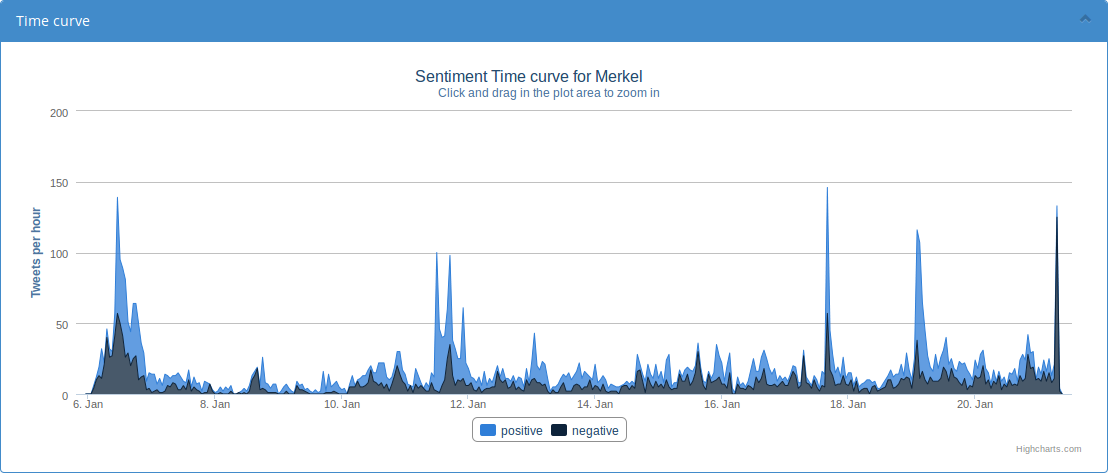
\includegraphics[width=0.8\textwidth]{Bilder/Frontend/Screenshots/sentimentPerHour-oldVersion.png}
\caption{Vorherige Version der Sentimentdarstellung im zeitlichen Verlauf.}
\label{img:SentOverTimeOld}
\end{figure} 

Daher wurde eine abweichende Darstellung entwickelt, welche das relative Verhältnis zwischen positiven und negativen Tweets darstellt. Dies ermöglicht dem Benutzer deutlich besser zu erkennen, wie sich das Meinungsbild zu dem jeweiligen Suchbegriff über den zeitlichen Verlauf entwickelt hat.

Aber auch bei dieser Darstellung gab es zwei verschiedene Probleme. Zum einen gab es unabhängig von der zeitlichen Auflösung immer einige Bereiche in denen es keine Tweets gab, weder positive noch negative, sodass viele Lücken in dem Graphen vorhanden waren, was es schwerer machte, diesen zu interpretieren. Zum anderen gab es ebenso Zeitpunkte, in denen nur positive oder nur negative Tweets gefunden werden konnten, sodass auch hierdurch die Darstellung stark zerhackt wurde. Diese Probleme wurden durch den Einsatz eines gleitenden Mittelwertes behoben. Der Graph zeigt somit zu jedem Zeitpunkt den Durchschnitt des Verhältnisses zwischen positiven und negativen Tweets der vorherigen 24 Stunden an.

\begin{figure}
 \centering
 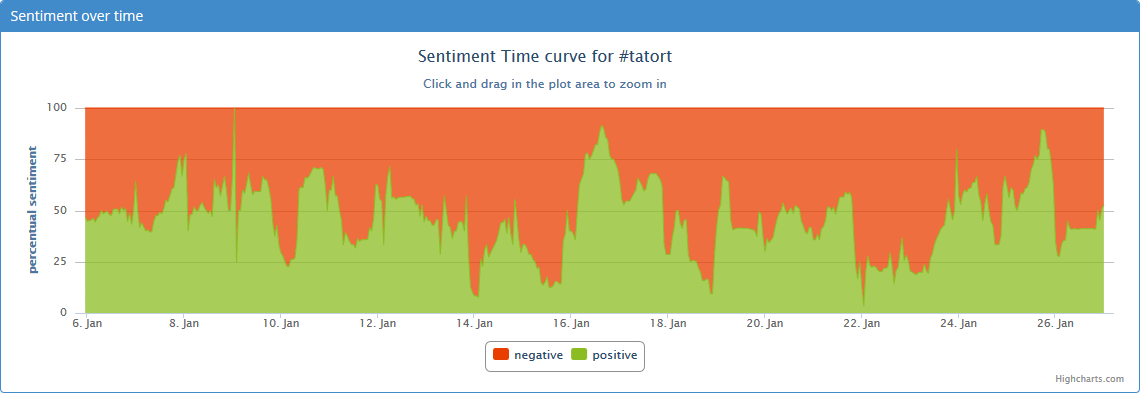
\includegraphics[width=0.8\textwidth]{Bilder/Frontend/Screenshots/latestSentimentPerHourTatort.png}
\caption{Finale Version der Sentimentdarstellung im zeitlichen Verlauf.}
\label{img:SentOverTimeFinal}
\end{figure} 

Diese Darstellung wurde von allen Beteiligten direkt verstanden und kann intuitiv auch ohne weitere Erklärungen von jedem Benutzer erfasst werden. (Siehe Abbildung \ref{img:SentOverTimeFinal}.)

\subsubsection{Performance der Tag Cloud}
Die Darstellung der Tag Cloud funktioniert wie gewünscht, es konnten jedoch Ladeprobleme bei den anderen Analysen beobachtet werden, seit die Tag Cloud zu den Auswertungen hinzugefügt wurde. Teilweise stockte die gesamte Darstellung der Auswertungen. Erste Überlegungen in Richtung Datenübertragung oder Verzögerungen auf Serverseite wurden schnell zerstreut, da andere Auswertungen hier länger auf Daten warten müssen und die Darstellung anderer Auswertungen hierdurch nicht verzögert wird.

Die weitere Analyse beschäftigte sich also mit dem Aufbau der eingesetzten Fremdkomponenten. Dies ergab, dass die \texttt{d3-cloud}-Bibliothek für jeden Eintrag einer Liste von Wörtern versucht, eine mögliche Position zu ermitteln. Diese Positionsermittlung geschieht in zentrischen Spiralen und benötigt dazu exakte Informationen über die Ausdehnung des jeweiligen Wortes, um auch die Lücken zwischen einzelnen unterschiedlich hohen Buchstaben des selben Wortes ausnutzen zu können. Versuche ergaben, dass sich unabhängig von der Länge dieser Liste die Anzahl der anzeigbaren Worte circa auf 100 belief. Obwohl der verfügbare Platz zur Anzeige ab dann nahezu vollständig aufgebraucht war, wurden genannte Berechnungen für jedes weitere Wort in der Liste vorgenommen. Diese Berechnungen konnten mittels kürzerer Listen als die Ursache für die beobachteten Probleme identifiziert werden. Obwohl mittels JavaScript-Timer- und Intervall-Funktionen versucht wurde für diese Berechnungen eine gewisse Asynchronität zu erreichen, sodass diese Berechnungen nicht mehr zwingend am Stück durchlaufen müssen, sondern von dem JavaScript-Interpreter unterbrochen werden können, um zunächst die anderen Auswertungen darzustellen, war dieser Ansatz von unzureichendem Erfolg gekrönt. Die Begrenzung der Liste schien das adäquate Mittel der Wahl zu sein, zusammen mit den Optimierungen in Punkto asychroner Ausführung konnte somit eine zufriedenstellende Performance-Optimierung erreicht werden, ohne durch eine zu große Beschränkung der Liste Nachteile im Detailgrad der Darstellung in Kauf nehmen zu müssen.

Zwischenzeitlich kam die Idee auf, die gesamte Berechnung evtl. auf den performanteren Server zu verlagern. Da die Darstellung der Tag Cloud aber von dem verfügbarem Platz auf der Webseite und vor allem auch von der verwendeten Schriftart abhängig ist, lässt sich diese Berechnung in zufriedenstellendem Maße nur im Browser bewerkstelligen.
Andernfalls hätte eine komplette Neuentwicklung der Tag Cloud stattfinden müssen, welche im Ergebnis fertige Grafiken zum Browser übertragen hätte und nicht wie es aktuell der Fall ist, lediglich eine schmale Liste von Wörtern im JSON-Format. Dieser Ansatz wurde daher auch sehr schnell wieder verworfen.

\subsubsection{Sprachfilter}
Die Idee der Einbindung eines Sprachfilters entstand, nachdem die Ansicht der Sprachverteilung implementiert war und der Kunde den Wunsch hegte, einzelne Sprachen eines Suchbegriffs genauer analysieren zu können. Der Sprachfilter ist eine globale Einstellung und wirkt sich auf die Auswertungen aller Suchbegriffe aus, die der Benutzer angezeigt bekommt.

Auf dieser Basis musste nun entschieden werden, wo in der Anzeige des Sprachfilters am besten einzubauen ist. In der ersten Version wurde ein einfaches Dropdown-Menü in der Navigationsleiste der Seite verwendet. Wie in Abbildung \ref{fig:langFilter1} zu sehen ist, war dieser Ansatz aber funktional getrieben, da die Anzeige des Sprachfilters nicht in das optische Gesamtkonzept integriert ist. Im zweiten Konzept (siehe \ref{fig:langFilter2}) fügt sich der Sprachfilter nun optisch ins Gesamtbild ein. Die Anbringung an die Suchleiste soll dem Benutzer suggerieren, dass es sich um eine Filterfunktion handelt und nicht um eine Einstellung der Anzeigesprache der Seite. Ein Problem ist allerdings, dass eine Änderung des Sprachfilters nur möglich ist, wenn die Suchleiste auch sichtbar ist. Da die Suchleiste aber verschwindet, wenn der Benutzer bei der Analyse der Ansichten nach unten scrollt, bedeutet dies, dass der Benutzer zunächst wieder nach oben scrollen muss, bevor der Sprachfilter geändert werden kann. Vor allem bei mobilen Endgeräten tritt dieses Problem aufgrund der geringeren Höhe der Ausgabe häufig auf. Aus dieser Überlegung entstand in der Folge das finale Konzept (siehe \ref{fig:langFilter3}), bei dem eine homogene Einbindung in die Navigationsleiste vorliegt. Daher ist der Sprachfilter auch immer sichtbar und verfügbar, da die Navigationsleiste beim Scrollen immer sichtbar bleibt.

\begin{figure}[ht]
\centering
\begin{subfigure}[t]{0.8\textwidth}

\includegraphics[width=\textwidth]{Bilder/Frontend/Screenshots/languageFilter1.png}
\caption{Erste Version des Sprachfilters. Ansatz: Funktionalität statt Design.}
\label{fig:langFilter1}
\end{subfigure}
\vspace*{5mm}
\begin{subfigure}[t]{0.8\textwidth}
\includegraphics[width=\textwidth]{Bilder/Frontend/Screenshots/languageFilter2.png}
\caption{Zweite Version des Sprachfilters. Ansatz: Sprachfilter an der Suchleiste.}
\label{fig:langFilter2}
\end{subfigure}
\vspace*{5mm}
\begin{subfigure}[t]{0.8\textwidth}
\includegraphics[width=\textwidth]{Bilder/Frontend/Screenshots/languageFilter3.png}
\caption{Finale Version des Sprachfilters. Ansatz: Integration in die Navigationsleiste}
\label{fig:langFilter3}
\end{subfigure}

\caption{Vergleich der verschiedenen Layouts des Sprachfilters}
\label{fig:langFilter}
\end{figure}

\subsubsection{Warnungen und Fehler}
Damit mögliche Fehler als Antwort einer Anfrage vom REST-Service nicht zum Absturz des gesamten Frontends führen, ist es notwendig, angemessen auf Fehler zu reagieren.
Wenn der HTTP Status Code der Antwort nicht \texttt{200 OK} lautet, handelt es sich um einen Fehler, bzw. ist ein Fehler im REST-Service aufgetreten. Eine Warnung liegt vor, wenn die Antwort vom REST-Service fehlerfrei vorliegt, aber nicht genügend Daten vorhanden sind, um vernünftige Auswertungen anzeigen zu können.

Die Anzeige der Fehler und Warnungen erfolgte zunächst in einer separaten Box, die aber nur die Anzeige eines einzigen Fehlers ermöglichte. Diese Einschränkung wurde getroffen, damit der Benutzer nicht von einer Flut an Fehlermeldungen erdrückt wird, falls die Verbindung zum REST-Service nicht fehlerfrei abläuft und somit jede Anfrage fehlschlägt.

Da aber Fehler und Warnungen immer mit einer Anfrage an den REST-Service verknüpft sind, erschien es im Laufe der Entwicklung vernünftig, dies auch optisch durch die Anzeige von Fehlern und Warnungen in den einzelnen Auswertungsboxen hervorzuheben. Fehlermeldungen, die nicht mit einer einzelnen Auswertung zusammenhängen, werden weiterhin in einer separaten Box angezeigt. Allerdings können diese Meldungen nun, ähnlich wie ein Fenster einer Anwendung in Windows, in der rechten oberen Ecke geschlossen werden, sodass der Benutzer selbst entscheiden kann, wann eine Meldung für ihn nicht mehr relevant ist.

Zusätzlich dazu wurden auch noch Fehlercodes eingeführt, die in den Fehlermeldungen angezeigt werden. Diese stellen einen Kompromiss zwischen möglichst exakter Fehlerbeschreibung für den Entwickler und Vermeidung unnötiger Details für den Benutzer dar.

\subsection{Diskussion}
Die Entwicklung des Frontend hat gezeigt, dass man diesen Teil nicht vollständig von der darunter liegenden Schicht loslösen kann und dass die Absprachen in unserem Fall mit dem REST-Service weit über eine Verständigung über die zu verwendende API hinausgehen müssen.
So muss man bei der Konzeption frühzeitig einige mögliche Problemstellen berücksichtigen, wie z.B. die auf im Schnitt maximal sechs mögliche parallele Verbindungen begrenzte Kapazität der Browser-Server-Verbindungen. Man sollte seine Anwendung also auf keinen Fall so bauen, dass man auf viele parallele Verbindungen angewiesen ist, und falls sich dies nicht vermeiden lässt, dass diese auf jeden Fall sehr schnell terminieren um weiterer Verbindungsversuche des Browsers nicht zu blockieren. Dies würde den Browser ansonsten schnell einfrieren oder der Benutzer erhält den Eindruck, dass seine Anwendung gerade hängen geblieben ist.
Diese Probleme lassen sich durch frühzeitige Konzepte wie z.B. einer Art Mulitplexing umgehen, welche hier nicht weiter ausgeführt werden sollen.

Des Weiteren haben wir erkannt, welche Berechnungen man browserseitig anstellen sollte und welche Berechnungen auf dem Server besser aufgehoben sind. Die Tag Cloud ist hier ein sehr schönes Beispiel. Aufgrund der Vielzahl unterschiedlicher Systeme, die auf einen Webservice zugreifen, kann man auf dem Server keinerlei Annahmen über die beim Besucher vorhandenen Schriftarten machen, welche browserseitig dynamisch für die Anzeige der Wörter verwendet werden. Somit lassen sich die exakten Positionen nicht auf dem Server ermitteln und diese Berechnung muss im Browser stattfinden. Dennoch sollte man sich an dieser Stelle stets der eingeschränkten Möglichkeiten von JavaScript bewusst sein, da zumindest zum heutigen Datum noch keine parallelen Ausführungen von Java\-Script möglich sind und zu umfangreiche Berechnungen den Browser sehr schnell blockieren können.
Eine sinnvolle Abwägung ist also unabdingbar.

Durch die verschiedenen optischen Ansätze des Frontends ist ebenfalls deutlich geworden, dass auch hier eine detaillierte konzeptionelle Vorarbeit notwendig ist, um spätere weiträumige Änderungen auf ein Minimum zu reduzieren. Weitreichende Änderungen bis hin zu kompletten Neuentwicklungen sind im Verlaufe eines Projektes oftmals sehr schwierig und dann nur mit einem erheblichen Mehraufwand zu bewerkstelligen. Dennoch hat der Verlauf des Projektes hier auch gezeigt, dass man selten im Voraus alle Anforderungen exakt kennt und gerade diese Komponente durch eine starke Nähe zum Kunden flexibel reagieren können muss. Frühzeitige Überlegungen gemeinsam mit dem Kunden, wie das Frontend aussehen soll und eventuell die Anfertigung eines funktionslosen Prototypen können mögliche Wege sein, unnötige Änderungen im späteren Verlauf zu vermeiden.
Dennoch kann man festhalten, dass die ändernden Anforderungen zusammen mit dem flexiblen Unterbau in Form des HTML5-Frameworks Bootstrap \cite{Bootstrap} zu einem sehr zufriedenstellenden Ergebnis geführt haben. Trotz aller Änderungen ist es uns daher gelungen, die gewünschten Anforderungen umzusetzen und sogar zu übertreffen.


\chapter{Ausblick und Fazit}
\label{cha:ausblick}
\label{sec:ausblick}
TMetrics ist ein System zur Datenanalyse von zu Suchbegriffen zugehörigen Tweets.
Neben dem Sammeln der Tweets ermöglicht TMetrics es dem Benutzer, sich die einzelnen Tweets 
anzeigen zu lassen und ihren Sentimentwert festzustellen.
Ebenfalls wird dem Benutzer die Möglichkeit geboten, sich Nachrichten eines Tages zu einem 
Begriff anzeigen zu lassen.
Zudem gibt es eine Anzeige der häufigsten Begriffe aller Tweets zu einem Suchbegriff ebenso 
wie die Anzeige der am häufigsten verwendeten Hashtags des Suchbegriffs.
Des Weiteren existiert noch die Möglichkeit, sich Cluster von Tweets anzeigen zu lassen.

Das gesamte System besteht aus einem Daemon, einem REST-Service und einem Frontend.
Der Daemon sucht permanent nach neuen Tweets zu vorgegebenen Suchbegriffen und speichert diese in einer lokalen Datenbank mitsamt berechnetem Sentiment ab. 
Der REST-Service beantwortet Anfragen, die vom Frontend aus durch den Benutzer gestellt werden, während das Frontend nur für die Darstellung der anzuzeigenden Daten zuständig ist.

Die Teilnehmer des Projektseminars sind mit dem Gesamtprodukt mit Ausnahme der mangelnden 
Performance zufrieden.
Das zu Beginn des Projektseminars angestrebte Ziel, ein System zur Datenanalyse von Tweets 
zu schaffen, wurde erreicht.
Zwar sind nicht alle geplanten Funktionalitäten wie eine Heatmap zu Suchbegriffen oder ein Kinomodul umgesetzt worden.
Aber dafür ist das Nachrichtenmodul als neue, zuvor nicht geplante Funktionalität hinzugekommen.

Die mangelnde Performance, die aufgrund der immer größer werdenden Datenmenge in der Datenbank auftritt, hat sich leider durch das gesamte Projektseminar hinweg durchgezogen. Es wurden viele Anstrengungen unternommen, diesen Mangel zu beheben. Dazu zählen
\begin{itemize}
\item das Anpassen des Datenbankschemas,
\item die Einführung von Indizes auf Tabellen innerhalb der Datenbank,
\item die Optimierung von SQL-Queries,
\item und ein effizienteres Arbeiten mit der Datenbank innerhalb des REST-Services und des Daemons.
\end{itemize}
Zwar haben all diese Änderungen teilweise eine enorme Verbesserung der Performance relativ zu vorher bewirkt, leider wurde aber dennoch nicht die von uns gewünschte Performance erreicht.

Retrospektiv stellte sich uns die Frage, ob die Entscheidung der Wahl einer relationalen Datenbank, in unserem Fall MySQL, nicht falsch gewesen ist, da in \cite[S.~24]{twitter_data_analytics} eine deutlich höhere Datenbankgeschwindigkeit mit einer NoSQL-Datenbank wie beispielsweise MongoDB \cite{mongodb} erreichbar zu sein scheint. Gerade beim Thema Big Data sollen NoSQL-Datenbanken gegenüber relationalen Datenbanken im Vorteil sein (\cite{seven_databases}, zitiert nach \cite[S.~23]{twitter_data_analytics}).
Vielleicht hätte aber auch ein anderes Datenbankschema bereits die angesprochene Performance radikal verbessert.

Zwar ist die Performance nicht zufriedenstellend, dafür aber funktionieren die einzelnen Komponenten wie Clustering, Sentimentanalyse und Nachrichtenmodul im gewünschten Umfang. Mögliche Optimierungen oder Probleme wurden bereits in den jeweiligen Abschnitten der genannten Komponenten erwähnt.

Trotzdem besteht weiterhin noch großes Ausbaupotential, was allerdings nicht enttäuschend, sondern vielmehr der abgedeckten Breite des Systems geschuldet ist.
Diese ermöglichte es nicht auch noch, die einzelnen Aspekte des Systems intensiver zu erweitern oder optimieren. Erweiterungsmöglichkeiten oder mögliche Optimierungsmaßnahmen wurden bereits in den Abschnitten über die einzelnen Aspekte des Systems behandelt.

Der Aufbau des Projektseminars durch Verwendung von Scrum als Entwicklungsmodell hat uns sehr geholfen, iterativ ein funktionierendes System zu schaffen, das mit jeder neuen Iteration erweitert und verbessert wurde.
Der wöchentliche Wechsel des Scrum-Masters hat jedem Teilnehmer zeitweise eine Verantwortung über das Projekt gegeben.
Somit ist jeder Einzelne in dieser Rolle dazu motiviert, sich mit dem Gesamtsystem auseinander zu setzen und mit den einzelnen Arbeitsbereichen zu kommunizieren, um gegebenenfalls auftretende Schwierigkeiten und Probleme früh zu erkennen.
Des Weiteren war das Planning Poker zum Einschätzen des Zeitaufwands hilfreich, um einen realistisches Ziel am Ende einer Iteration anzustreben und zu erreichen.
Die Verwendung eines Scrum-Boards ermöglichte es jedem Teilnehmer, immer zu sehen, wie weit das Projekt innerhalb der Iteration bereits fortgeschritten und an welchen Stellen gegebenenfalls noch weitere Hilfe nötig war.

Die Stimmung unter allen Teilnehmern war immer gut, sodass ein harmonisches und motivierendes Arbeitsklima entstand, das die Produktivität gesteigert hat.
Insgesamt haben während des Projektseminars alle Teilnehmer viel Neues gelernt, sei es über das Entwickeln mithilfe von Scrum, die Versionierungskontrolle durch Git, besondere Tricks in JavaScript, mögliche Stolpersteine bei der Multi-Threading-Entwicklung, die Verwendung eines Build-Management-Tools wie Maven, das Einrichten eines Servers und vieles mehr, was in Hinblick auf zukünftige (berufliche) Projekte hilfreich sein wird.

\addcontentsline{toc}{chapter}{Literaturverzeichnis}
	\bibliographystyle{gerplain}
% 	\bibliography{kmeansPaper}
	\bibliography{references}
%\addcontentsline{toc}{chapter}{Abbildungsverzeichnis}
%	\listoffigures
%\addcontentsline{toc}{chapter}{Tabellenverzeichnis}
%	\listoftables
%\addcontentsline{toc}{chapter}{Stichwortverzeichnis}
%	\renewcommand{\indexname}{Stichwortverzeichnis} 
	\printindex

\appendix

\chapter{REST API}
\def \tweite {10.1cm}
%\section*{REST-API}
\subsection*{Query-Methoden}
\textbf{POST \texttt{/queries/post}}
\begin{table}[h!]
\begin{tabular}{| c | p{\tweite} | l |}
\hline
	\textbf{Parameter} & \textbf{Beschreibung} &  \\
\hline \hline
 	\texttt{q} & Suchbegriff & verpflichtend \\
\hline
\end{tabular}
\end{table}
\newline
Legt einen noch nicht existierenden Suchbegriff in der Datenbank an.
\newline
 \newline
\textbf{POST \texttt{/queries/postPriority}}
\begin{table}[h!]
\begin{tabular}{| c | p{\tweite} | l |}
\hline
	\textbf{Parameter} & \textbf{Beschreibung} &  \\
\hline \hline
 	\texttt{id} & ID eines vorhandenen Suchbegriffs & verpflichtend \\
\hline
 	\texttt{p} & Neue Priorität für den angegebenen Suchbegriff & verpflichtend \\
\hline
\end{tabular}
\end{table}
\newline
Ändert die User-Priorität für einen Suchbegriff.
\newline
 \newline
\textbf{POST \texttt{/queries/postActiveFlag}}
\begin{table}[h!]
\begin{tabular}{| c | p{\tweite} | l |}
\hline
	\textbf{Parameter} & \textbf{Beschreibung} &  \\
\hline \hline
 	\texttt{id} & ID eines vorhandenen Suchbegriffs & verpflichtend \\
\hline
 	\texttt{active} & True oder false, je nachdem ob der Suchbegriff für den Daemon aktiv oder inaktiv sein soll (verpflichtend) & verpflichtend \\
\hline
\end{tabular}
\end{table}
\newline
Aktiviert oder deaktiviert einen Suchbegriff für den Daemon.
\newpage

\noindent
\textbf{GET \texttt{/queries/byid}}
\begin{table}[h!]
\begin{tabular}{| c | p{\tweite} | l |}
\hline
	\textbf{Parameter} & \textbf{Beschreibung} &  \\
\hline \hline
 	\texttt{id} & ID eines Suchbegriffs & verpflichtend \\
\hline
\end{tabular}
\end{table}
\newline
Liefert den durch die ID spezifizierten Suchbegriff aus der Datenbank zurück, falls vorhanden.

\noindent
\textbf{GET \texttt{/queries/bystring}}
\begin{table}[h!]
\begin{tabular}{| c | p{\tweite} | l |}
\hline
	\textbf{Parameter} & \textbf{Beschreibung} &  \\
\hline \hline
 	\texttt{q} & Suchbegriff & verpflichtend \\
\hline
\end{tabular}
\end{table}
\newline
Liefert den angegebenen Suchbegriff aus der Datenbank (inklusive ID) zurück, falls vorhanden.

\begin{figure}[h!]
\includegraphics[scale=0.6]{Bilder/RestApi/queriesByString.png}
\end{figure}

\noindent
\textbf{GET \texttt{/queries/contains}}
\begin{table}[h!]
\begin{tabular}{| c | p{\tweite} | l |}
\hline
	\textbf{Parameter} & \textbf{Beschreibung} &  \\
\hline \hline
 	\texttt{q} & Suchbegriff & verpflichtend \\
\hline
\end{tabular}
\end{table}
\newline
Liefert zurück, ob der angegebene Suchbegriff in der Datenbank vorhanden ist.

\noindent
\textbf{GET \texttt{/queries/suggestions}}
\begin{table}[h!]
\begin{tabular}{| c | p{\tweite} | l |}
\hline
	\textbf{Parameter} & \textbf{Beschreibung} &  \\
\hline \hline
 	\texttt{q} & Beginn eines Suchbegriffs & verpflichtend \\
\hline
\end{tabular}
\end{table}
\newline
Liefert eine Liste der Suchbegriffe in der Datenbank zurück, welche mit \texttt{q} beginnen. Die Liste ist absteigend nach Anzahl Vorkommnisse sortiert. Es werden maximal fünf Ergebnisse zurückgeliefert.
\newpage

\noindent
\textbf{GET \texttt{/queries/metadata}}
\begin{table}[h!]
\begin{tabular}{| c | p{\tweite} | l |}
\hline
	\textbf{Parameter} & \textbf{Beschreibung} &  \\
\hline \hline
 	\texttt{id} & ID eines Suchbegriffs & verpflichtend \\
\hline
 	\texttt{lang} & Sprache der einbezogenen Tweets im ISO-Format & optional \\
\hline
\end{tabular}
\end{table}
\newline
Liefert die Metadaten des Suchbegriffs dieser \texttt{id} zurück:
\begin{figure}[h!]
\includegraphics[scale=0.6]{Bilder/RestApi/queriesMetadata.png}
\end{figure}

\noindent
\textbf{GET \texttt{/queries/hasDaemonFetched}}
\begin{table}[h!]
\begin{tabular}{| c | p{\tweite} | l |}
\hline
	\textbf{Parameter} & \textbf{Beschreibung} &  \\
\hline \hline
 	\texttt{id} & ID eines Suchbegriffs & verpflichtend \\
\hline
\end{tabular}
\end{table}
\newline
Überprüft, ob der Daemon für den Suchbegriff mit der angegebenen \texttt{id}, Tweets gefunden hat.
\newpage

\subsection*{Result-Methoden}
\noindent
\textbf{GET \texttt{/results/tweet}}
\begin{table}[h!]
\begin{tabular}{| c | p{\tweite} | l |}
\hline
	\textbf{Parameter} & \textbf{Beschreibung} &  \\
\hline \hline
 	\texttt{id} & ID eines Tweets & verpflichtend \\
\hline
\end{tabular}
\end{table}
\newline
Liefert alle Informationen für den Tweet dieser \texttt{id} aus der Datenbank.

\noindent
\textbf{GET \texttt{/results/tweets}}
\begin{table}[h!]
\begin{tabular}{| c | p{10.1cm} | l |}
\hline
	\textbf{Parameter} & \textbf{Beschreibung} &  \\
\hline \hline
 	\texttt{id} & ID eines Suchbegriffs & verpflichtend \\
\hline
 	\texttt{sent} & Sentiment: liefert nur Tweets mit diesem Sentiment zurück, erlaubte Eingaben: "`positive"', "`neutral"', "`negative"' (alle Tweets falls nicht angegeben) & optional \\
\hline
 	\texttt{start} & Datum im Format YYYY-DD-MMTHH:MM:SS, Datum des ältesten zurückgegebenen Tweets (keine untere Grenze falls nicht angegeben) & optional \\
\hline
 	\texttt{end} & Datum im Format YYYY-DD-MMTHH:MM:SS, Datum des neuesten zurückgegebenen Tweets (keine obere Grenze falls nicht angegeben) & optional \\
\hline
 	\texttt{lang} & Sprache der Tweets im ISO-Format wie von Twitter erkannt (alle Tweets falls nicht angegeben) &  optional\\
\hline
 	\texttt{limit} & Anzahl zurückgelieferter Tweets (100 falls nicht angegeben) & optional \\
\hline
\end{tabular}
\end{table}
\newline
Liefert die Tweets, die dem Suchbegriff dieser \texttt{id} zugeordnet sind, unter den angegebenen Einschränkungen.

\includegraphics[scale=0.6]{Bilder/RestApi/GetTweet.png}

\noindent
\textbf{GET \texttt{/results/user}}
\begin{table}[h!]
\begin{tabular}{| c | p{\tweite} | l |}
\hline
	\textbf{Parameter} & \textbf{Beschreibung} &  \\
\hline \hline
 	\texttt{id} & ID eines Twitter-Users & verpflichtend \\
\hline
\end{tabular}
\end{table}
\newline
Liefert alle Informationen für den User dieser \texttt{id} aus der Datenbank.

\newpage
\noindent
\textbf{GET \texttt{/results/sentimentPerHour}}
\begin{table}[h!]
\begin{tabular}{| c | p{\tweite} | l |}
\hline
	\textbf{Parameter} & \textbf{Beschreibung} &  \\
\hline \hline
 	\texttt{id} & ID eines Suchbegriffs & verpflichtend \\
\hline
 	\texttt{lang} & Sprache der angezeigten Tweets (alle Tweets falls nicht angegeben) & optional \\
\hline
\end{tabular}
\end{table}
\newline
Liefert für jede volle Stunde die Anzahl positiver und negativer Posts zum Suchbegriff mit dieser \texttt{id} zurück.

\noindent
\textbf{GET \texttt{/results/countPerHour}}
\begin{table}[h!]
\begin{tabular}{| c | p{\tweite} | l |}
\hline
	\textbf{Parameter} & \textbf{Beschreibung} &  \\
\hline \hline
 	\texttt{id} & ID eines Suchbegriffs & verpflichtend \\
\hline
 	\texttt{lang} & Sprache der angezeigten Tweets (alle Tweets falls nicht angegeben) & optional \\
\hline
\end{tabular}
\end{table}
\newline
Liefert für jede volle Stunde die Anzahl Posts zum Suchbegriff mit dieser \texttt{id} zurück.

\includegraphics[scale=0.6]{Bilder/RestApi/resultsCountPerHour.png}

\newpage
\noindent
\textbf{GET \texttt{/results/tagCloud}}
\begin{table}[h!]
\begin{tabular}{| c | p{\tweite} | l |}
\hline
	\textbf{Parameter} & \textbf{Beschreibung} &  \\
\hline \hline
 	\texttt{id} & ID eines Suchbegriffs & verpflichtend \\
\hline
 	\texttt{lang} & Sprache der angezeigten Tweets (alle Tweets falls nicht angegeben) & optional \\
\hline
 	\texttt{count} &  Anzahl einbezogener Tweets (100 falls nicht angegeben) & optional \\
\hline
\end{tabular}
\end{table}
\newline
Liefert den konkatenierten Text der festgelegten Anzahl Tweets zum Suchbegriff der angegebenen \texttt{id} zurück, sodass damit auf Client-Seite die Tag-Cloud erstellt werden kann.

\noindent
\textbf{GET \texttt{/results/sentiments}}
\begin{table}[h!]
\begin{tabular}{| c | p{\tweite} | l |}
\hline
	\textbf{Parameter} & \textbf{Beschreibung} &  \\
\hline \hline
 	\texttt{id} & ID eines Suchbegriffs & verpflichtend \\
\hline
 	\texttt{lang} & Sprache der angezeigten Tweets (alle Tweets falls nicht angegeben) & optional \\
\hline
\end{tabular}
\end{table}
\newline
Durchsucht die Tweets zum Suchbegriff mit der angegebenen \texttt{id} und liefert zurück, wieviele von ihnen jeweils das Sentiment "`positiv"', "`neutral"' und "`negativ"' haben.
\begin{figure}[h!]
\includegraphics[scale=0.6]{Bilder/RestApi/resultsSentiment.png}
\end{figure}

\noindent
\textbf{GET \texttt{/results/getDataGroups}}
\begin{table}[h!]
\begin{tabular}{| c | p{\tweite} | l |}
\hline
	\textbf{Parameter} & \textbf{Beschreibung} &  \\
\hline \hline
 	\texttt{id} & ID eines Suchbegriffs & verpflichtend \\
\hline
 	\texttt{lang} & Sprache der angezeigten Tweets (alle Tweets falls nicht angegeben) & optional \\
\hline
\end{tabular}
\end{table}
\newline
Durchsucht die Tweets zum Suchbegriff mit der angegebenen \texttt{id} und liefert zurück, welcher Tweet zu welchem Cluster gehört.

\newpage
\noindent
\textbf{GET \texttt{/results/peaks}}
\begin{table}[h!]
\begin{tabular}{| c | p{\tweite} | l |}
\hline
	\textbf{Parameter} & \textbf{Beschreibung} &  \\
\hline \hline
 	\texttt{id} & ID eines Suchbegriffs & verpflichtend \\
\hline
 	\texttt{lang} & Sprache der angezeigten Tweets (alle Tweets falls nicht angegeben) & optional \\
\hline
\end{tabular}
\end{table}
\newline
Liefert die Peaks des Suchbegriffs dieser \texttt{id} zurück.

\noindent
\textbf{GET \texttt{/results/news}}
\begin{table}[h!]
\begin{tabular}{| c | p{\tweite} | l |}
\hline
	\textbf{Parameter} & \textbf{Beschreibung} &  \\
\hline \hline
 	\texttt{id} & ID eines Suchbegriffs & verpflichtend \\
\hline
 	\texttt{lang} & Sprache der angezeigten Tweets (alle Tweets falls nicht angegeben) & optional \\
\hline
 	 \texttt{day} &  Tag für den die News abzufragen sind & optional \\
\hline
 	 \texttt{month} & Monat für den die News abzufragen sind & optional \\
\hline
 	 \texttt{year} & Jahrg für den die News abzufragen sind & optional \\
\hline
\end{tabular}
\end{table}
\newline
Liefert die News des Suchbegriffs dieser \texttt{id} für den angegebenen Zeitraum zurück:
\begin{figure}[h!]
\includegraphics[scale=0.6]{Bilder/RestApi/resultNews.png}
\end{figure}

\newpage
\noindent
\textbf{GET \texttt{/results/languages}}
\begin{table}[h!]
\begin{tabular}{| c | p{\tweite} | l |}
\hline
	\textbf{Parameter} & \textbf{Beschreibung} &  \\
\hline \hline
 	\texttt{id} & ID eines Suchbegriffs & verpflichtend \\
\hline
\end{tabular}
\end{table}
\newline
Gibt eine Liste von Sprachen zurück (eine Sprache besteht aus isoCode und Häufigkeit).

\includegraphics[scale=0.6]{Bilder/RestApi/resultLanguages.png}

\noindent
\textbf{GET \texttt{/results/trainingTweets}}
\begin{table}[h!]
\begin{tabular}{| c | p{\tweite} | l |}
\hline
	\textbf{Parameter} & \textbf{Beschreibung} &  \\
\hline \hline
 	\texttt{feature} & Betrachtetes Feature & verpflichtend \\
\hline
 	\texttt{lang} & Sprache des Modells & optional \\
\hline
\end{tabular}
\end{table}
\newline
Gibt eine Liste von Tweets zurück, die das angegebene Feature für die spezifizierte Sprache am meißten beeinflusst haben.

\noindent
\textbf{GET \texttt{/results/hashtagstatistics}}
\begin{table}[h!]
\begin{tabular}{| c | p{\tweite} | l |}
\hline
	\textbf{Parameter} & \textbf{Beschreibung} &  \\
\hline \hline
 	\texttt{id} & ID eines Suchbegriffs & verpflichtend \\
\hline
 	\texttt{lang} & Sprache der angezeigten Tweets (alle Tweets falls nicht angegeben) & optional \\
\hline
\end{tabular}
\end{table}
\newline
Durchsucht die Tweets zum Suchbegriff mit der angegebenen \texttt{id} und liefert zurück, welcher Hashtags darin vorkommen. Die Ausgabe ist sortiert nach den Häufigkeiten.
\begin{figure}[h!]
\includegraphics[scale=0.6]{Bilder/RestApi/resultsHashtagStatistics.png}
\end{figure}


\end{document}
